\documentclass[11pt]{book}

\setlength{\oddsidemargin}{0.1in}
\setlength{\evensidemargin}{0.1in}
\setlength{\textwidth}{6.5in}
\setlength{\topmargin}{.04in}
\setlength{\textheight}{8.2in}

%Path to images
\usepackage{graphicx}
\graphicspath{ {figures/} }
\DeclareGraphicsExtensions{.eps,.png}

%% AMS packages

\usepackage{amsmath,amsfonts,amssymb,amsthm}

%% other packages
% note that "epstopdf" is required for Mac users

\usepackage{graphics,epstopdf,fancyhdr,palatino, verbatim, bigstrut, lscape, enumerate, caption}
\usepackage{graphicx, animate}
\usepackage{color, colortbl}
\definecolor{tracered}{rgb}{1,0.5,0.5}
\definecolor{traceblue}{rgb}{0.5,0.5,1}
\usepackage{makeidx}
\makeindex

\usepackage{hyperref}
\hypersetup{colorlinks=true, linkcolor=blue,  anchorcolor=blue,
citecolor=blue, filecolor=blue, menucolor=blue, pagecolor=blue,
urlcolor=blue,pdftitle={ACmain}}

%% Packages to use the MathDesign _Charter_ font.

%\usepackage[T1]{fontenc}
%\usepackage[charter]{mathdesign}

%% Activities package

% Options to the activities package are: "bighints", "smallhints",
% "activitysolutions" (which are mutually exclusive; the last one listed is the
% one used) "exercisesolutions", and "authornotes".  If the option is there, then
% the corresponding environment is shown.

\usepackage{activities}

\lhead[\fancyplain{}{\thepage}]         {\fancyplain{}{\rightmark}}
\chead[\fancyplain{}{}]                 {\fancyplain{}{}}
\rhead[\fancyplain{}{\rightmark}]       {\fancyplain{\scalebox{0.35}{\includegraphics{figures/CClicense.eps}} }{\thepage}}

\rfoot[\fancyplain{}{}] {\fancyplain{}{\scalebox{0.35}{\includegraphics{figures/CClicense.eps}} }}

\cfoot[\fancyplain{\thepage}{}] {\fancyplain{\thepage}{}}

\lfoot[ \fancyplain{ \scalebox{0.35}{\includegraphics{figures/CClicense.eps}}  }  { \scalebox{0.35}{\includegraphics{figures/CClicense.eps}}  } ] {\fancyplain{}{}}

\newcounter{cnt}
\newenvironment{numlist}{\begin{list}{(\arabic{cnt})}{\usecounter{cnt}
\setlength{\leftmargin}{.35 in}\setlength{\labelwidth}{.35 in}
\setlength{\itemsep}{10 pt}}}{\end{list}}

\newcounter{cnt4}
\newenvironment{numlist2}{\begin{list}{(\arabic{cnt4})}{\usecounter{cnt4}
\setlength{\leftmargin}{.5 in}\setlength{\labelwidth}{.25 in}
\setlength{\itemsep}{10 pt}}}{\end{list}}

\newcounter{cnt2}
\newenvironment{alphalist}{\vspace*{-3 pt}\begin{list}{(\alph{cnt2})}{\usecounter{cnt2}
\setlength{\leftmargin}{.5 in}\setlength{\labelwidth}{.25
in}\setlength{\itemsep}{5 pt}}}{\end{list}}

\newcounter{cnt3}
\newenvironment{alphalist2}{\vspace*{-3 pt}\begin{list}{(\alph{cnt3})}{\usecounter{cnt3}
\setlength{\leftmargin}{.25 in}\setlength{\labelwidth}{.25
in}\setlength{\itemsep}{5 pt}}}{\end{list}}

\newcounter{cnt5}
\newenvironment{thmlist}{\vspace*{-3 pt}\begin{list}{{\em (\roman{cnt5})}}{\usecounter{cnt5}
\setlength{\leftmargin}{.5 in}\setlength{\labelwidth}{.25
in}\setlength{\itemsep}{3 pt}}}{\end{list}}

%\newcommand{\lint}{\raisebox{-.14 in}{\underline{\hspace*{.7 ex}}}
%\hspace*{-1 ex} \int}

%\newcommand{\uint}{\hspace*{1.5 ex} \raisebox{.296 in}{\underline{\hspace*{.7 ex}}}
%\hspace*{-2.3 ex} \int}

\setlength{\parskip}{5 pt}

\newcounter{lastenum}
\newcommand{\saveCount}{\setcounter{lastenum}{\value{enumi}}}
\newcommand{\restoreCount}{\setcounter{enumi}{\value{lastenum}}}

\newcommand{\be}{\begin{numlist}}
\newcommand{\ee}{\end{numlist}}
\newcommand{\bei}{\begin{numlist2}}
\newcommand{\eei}{\end{numlist2}}
\newcommand{\ba}{\begin{alphalist}}
\newcommand{\ea}{\end{alphalist}}
\newcommand{\bal}{\begin{alphalist2}}
\newcommand{\eal}{\end{alphalist2}}
\newcommand{\bi}{\begin{itemize}}
\newcommand{\ei}{\end{itemize}}
\newcommand{\btl}{\begin{thmlist}}
\newcommand{\etl}{\end{thmlist}}


\newcommand{\R}{\mathbb{R}}
\newcommand{\va}{\mathbf{a}}
\newcommand{\vb}{\mathbf{b}}
\newcommand{\vc}{\mathbf{c}}
\newcommand{\ve}{\mathbf{e}}
\newcommand{\vi}{\mathbf{i}}
\newcommand{\vj}{\mathbf{j}}
\newcommand{\vk}{\mathbf{k}}
\newcommand{\vn}{\mathbf{n}}
\newcommand{\vm}{\mathbf{m}}
\newcommand{\vr}{\mathbf{r}}
\newcommand{\vs}{\mathbf{s}}
\newcommand{\vu}{\mathbf{u}}
\newcommand{\vv}{\mathbf{v}}
\newcommand{\vw}{\mathbf{w}}
\newcommand{\vx}{\mathbf{x}}
\newcommand{\vy}{\mathbf{y}}
\newcommand{\vz}{\mathbf{z}}
\newcommand{\vzero}{\mathbf{0}}
\newcommand{\vF}{\mathbf{F}}
\newcommand{\vR}{\mathbf{R}}
\newcommand{\vT}{\mathbf{T}}
\newcommand{\vL}{\mathbf{L}}
\newcommand{\proj}{\text{proj}}
\newcommand{\comp}{\text{comp}}


% theorem-like environments
\theoremstyle{definition}
\newtheorem{pa}{Preview Activity}[chapter]
\newtheorem{example}{Example}[chapter]
\newtheorem{definition}{Definition}[chapter]

\newcommand{\bex}{\begin{center}\underline{\hspace{5.0in}}\end{center} \begin{example}}
\newcommand{\eex}{\end{example} \noindent{\bf Solution.}~~}
\newcommand{\afterex}{\begin{center}\underline{\hspace{5.0in}}\end{center}}
\newcommand{\afterexercises}{\nin \hrulefill \vfill \ \newpage}

% my commands

\newcommand{\ds}{\ensuremath{\displaystyle}}
\newcommand{\nin}{\noindent}
\newcommand{\tr}{\vspace*{0.5in}}
\newcommand{\lr}{\vspace*{1.0in}}
\newcommand{\mr}{\vspace*{2.0in}}
\newcommand{\br}{\vspace*{3.0in}}
\newcommand{\afterpa}{\hfill $\bowtie$}
\newcommand{\aftera}{\hfill $\lhd$}

\newcommand\T{\rule{0pt}{2.6ex}}
\newcommand\B{\rule[-1.2ex]{0pt}{0pt}}

\newenvironment{goals}{ \vspace*{7 pt}{\large \textbf{Motivating Questions}} \vspace*{-6 pt} \\ ~\hrule~ \vspace*{2 pt}

 {\em In this section, we strive to understand the ideas generated by the following important questions:}
\vspace*{-5 pt} \\ ~\hrule~ \vspace*{-3 pt}
\begin{list}{\labelitemi}{\leftmargin=1.25em}
\setlength{\itemsep}{3 pt}}{ \end{list} \vspace*{-2 pt}}

\newenvironment{summary}{ %\vspace*{7 pt}
\nin{\large \textbf{Summary}} \vspace*{-6 pt} \\ ~\hrule~ \vspace*{2 pt}
\nin{\em \hspace*{-10pt} In this section, we encountered the following important ideas:}
\vspace*{-9 pt} \\ ~\hrule~ \vspace*{-3 pt}
\begin{list}{\labelitemi}{\leftmargin=1.25em}
\setlength{\itemsep}{3 pt}}{ \end{list} \vspace*{-2 pt}}

\pagestyle{fancyplain}

\setcounter{chapter}{8}

%TABLE/GRAPH ON ONE LINE COMMANDS
%\begin{figure}[h]
%\centering
%\begin{tabular}{cc}
%	\raisebox{.75in}{\begin{tabular}[b]{c|c} $x$ & $y$ \\ \hline a & b \\ c & d \\ e & f  \end{tabular} } &	
%	\hspace{1in} \includegraphics[2in,2in]{c:/mth310/project/Hamilton.bmp}
%\end{tabular}
%\caption{{\scriptsize Table and graph for $f$.}}
%\end{figure}

%%%%%%%%%%%%%%%%%%%%%%%%%%%%%%%%%%%%%%%%%%%%%%%%%%%%

\title{Active Calculus \\ \vspace{0.1in} \scalebox{0.75}{\includegraphics{figures/CClicense.eps}}}
%\date{\today}
\author{Steve Schlicker, Lead Author and Editor \\ Department of Mathematics \\ Grand Valley State University \\
\texttt{schlicks@gvsu.edu} \\
\href{http://faculty.gvsu.edu/schlicks/}{\texttt{http://faculty.gvsu.edu/schlicks/}}\\
\vspace{1.5in} \\
David Austin, Contributing Author \\
\href{http://merganser.math.gvsu.edu/david/}{\texttt{http://merganser.math.gvsu.edu/david/}} \\ \ \\
Matt Boelkins, Contributing Author \\
\href{http://faculty.gvsu.edu/boelkinm/}{\texttt{http://faculty.gvsu.edu/boelkinm/}} }

%\includeonly{6.chap}

\begin{document}
\frontmatter
\maketitle
\tableofcontents

%\chapter{Preface} 

\section*{A free and open-source calculus \ \scalebox{0.5}{\includegraphics{figures/CClicense.eps}}} 

\vspace*{-0.15in}

As we have noted in the single-variable edition of \emph{Active Calculus}, several fundamental ideas in calculus are more than 2000 years old, and calculus as a formal subdiscipline of mathematics was first introduced and developed in the late 1600s.  Mathematicians agree that the subject has been understood -- rigorously and by experts -- since the mid 1800s.  The discipline is one of our great human intellectual achievements.

While each author of a calculus textbook certainly offers her own creative perspective on the subject, it is hardly the case that many of the ideas she presents are new.  Indeed, the mathematics community broadly agrees on what the main ideas of calculus are, as well as their justification and their importance; the core parts of nearly all calculus textbooks are very similar.  As such, it is our opinion that in the 21st century -- an age where the internet permits seamless and immediate transmission of information -- no one should be required to purchase a calculus text to read, to use for a class, or to find a coherent collection of problems to solve.  Calculus belongs to humankind, not any individual author or publishing company.  Thus, a main purpose of this work is to present a new multivariable calculus text that is \emph{free}.  In addition, instructors who are looking for a multivariable calculus text should have the opportunity to download the source files and make modifications that they see fit; thus this text is \emph{open-source}.  %Since August 2013, \emph{Active Calculus} has been endorsed by the American Institute of Mathematics and its Open Textbook Initiative: \href{http://aimath.org/textbooks/}{\texttt{http://aimath.org/textbooks/}}.

Any professor or student may use an electronic version of the text for no charge.  A .pdf copy of the text may be obtained by download from the \href{http://faculty.gvsu.edu/boelkinm/Home/Active_Calculus.html}{Active Calculus home page}, or directly from
\begin{center} \href{http://gvsu.edu/s/Wb}{\texttt{http://gvsu.edu/s/Wb}}. \end{center}  
Because the text is open-source, any instructor may acquire the full set of source files, by request via email to Matt Boelkins.  

This work is licensed under the Creative Commons Attribution-NonCommercial-ShareAlike 3.0 Unported License.  The graphic 
\begin{center}
\includegraphics{figures/CClicense.eps}
\end{center}
that appears throughout the text shows that the work is licensed with the Creative Commons, that the work may be used for free by any party so long as attribution is given to the author(s), that the work and its derivatives are used in the spirit of ``share and share alike,'' and that no party may sell this work or any of its derivatives for profit.  Full details may be found by visiting
\begin{center}
\href{http://creativecommons.org/licenses/by-nc-sa/3.0/}{\texttt{http://creativecommons.org/licenses/by-nc-sa/3.0/}}
\end{center} 
or sending a letter to Creative Commons, 444 Castro Street, Suite 900, Mountain View, California, 94041, USA. 

\section*{Active Calculus - Multivariable: our goals}

In \emph{Active Calculus - Multivariable}, we endeavor to actively engage students in learning the subject through an activity-driven approach in which the vast majority of the examples are completed by students.  Where many texts present a general theory of calculus followed by substantial collections of worked examples, we instead pose problems or situations, consider possibilities, and then ask students to investigate and explore.  Following key activities or examples, the presentation normally includes some overall perspective and a brief synopsis of general trends or properties, followed by formal statements of rules or theorems.  While we often offer plausibility arguments for such results, rarely do we include formal proofs.  It is not the intent of this text for the instructor or author to \emph{demonstrate} to students that the ideas of calculus are coherent and true, but rather for students to \emph{encounter} these ideas in a supportive, leading manner that enables them to begin to understand for themselves why calculus is both coherent and true.  

This approach is consistent with the following goals:

\begin{itemize}
   \item To have students engage in an active, inquiry-driven approach, where learners strive to construct solutions and approaches to ideas on their own, with appropriate support through questions posed, hints, and guidance from the instructor and text.
   \item To build in students intuition for why the main ideas in multivariable calculus are natural and true.  We strive to accomplish this by using specific cases to highlight the ideas for the general situation using contexts that are common and familiar.
   \item To challenge students to acquire deep, personal understanding of multivariable calculus through reading the text and completing preview activities on their own, through working on activities in small groups in class, and through doing substantial exercises outside of class time.  
   \item To strengthen students' written and oral communicating skills by having them write about and explain aloud the key ideas of multivariable calculus.
\end{itemize}

\section*{Features of the Text}

Similar to the presentation of the single-variable \emph{Active Calculus}, instructors and students alike will find several consistent features in the presentation, including:

\begin{itemize}
	\item {\bf Motivating Questions.}  At the start of each section, we list \emph{motivating questions} that provide motivation for why the following material is of interest to us.  One goal of each section is to answer each of the motivating questions.
	\item {\bf Preview Activities.} Each section of the text begins with a short introduction, followed by a \emph{preview activity}.  This brief reading and the preview activity are designed to foreshadow the upcoming ideas in the remainder of the section; both the reading and preview activity are intended to be accessible to students \emph{in advance} of class, and indeed to be completed by students before a day on which a particular section is to be considered.
	\item {\bf Activities.}  Every section in the text contains several \emph{activities}.  These are designed to engage students in an inquiry-based style that encourages them to construct solutions to key examples on their own, working either individually or in small groups.  
	\item {\bf Exercises.}  There are dozens of calculus texts with (collectively) tens of thousands of exercises.  Rather than repeat standard and routine exercises in this text, we recommend the use of WeBWorK with its access to the National Problem Library and its many multivariable calculus problems.  In this text, there are a small number of challenging exercises in each section.  Almost every such exercise has multiple parts, requires the student to connect several key ideas, and expects that the student will do at least a modest amount of writing to answer the questions and explain their findings.  For instructors interested in a more conventional source of exercises, consider the freely available text by Gilbert Strang of MIT, available in .pdf format from the MIT open courseware site via \href{http://gvsu.edu/s/bh}{\texttt{http://gvsu.edu/s/bh}}.
	\item {\bf Graphics.}  As much as possible, we strive to demonstrate key fundamental ideas visually, and to encourage students to do the same.  Throughout the text, we use full-color graphics to exemplify and magnify key ideas, and to use this graphical perspective alongside both numerical and algebraic representations of calculus.  The figures and the software to generate them have been created by David Austin.
	\item {\bf Links to Java Applets.}  Many of the ideas of multivariable calculus are best understood dynamically, and there are a number of applets referenced in the text that can be used by instructors and students to assist in the investigations and demonstrations. The use of these freely available applets is in accord with our philosophy that no one should be required to purchase materials to learn calculus. We are indebted to everyone who allows their expertise to be openly shared. 
	\item {\bf Summary of Key Ideas.}  Each section concludes with a summary of the key ideas encountered in the preceding section; this summary normally reflects responses to the motivating questions that began the section.
\end{itemize}


\section*{How to Use this Text}

This text may be used as a stand-alone textbook for a standard multivariable calculus course or as a supplement to a more traditional text. 

\subsection*{Electronically}

Because students and instructors alike have access to the book in .pdf format, there are several advantages to the text over a traditional print text.  One is that the text may be projected on a screen in the classroom (or even better, on a whiteboard) and the instructor may reference ideas in the text directly, add comments or notation or features to graphs, and indeed write right on the text itself.  Students can do likewise, choosing to print only whatever portions of the text are needed for them.  In addition, the electronic version of the text includes live html links to java applets, so student and instructor alike may follow those links to additional resources that lie outside the text itself.  Finally, students can have access to a copy of the text anywhere they have an internet-enabled device.

\subsection*{Activities Workbook}

Each section of the text has a preview activity and at least three in-class activities embedded in the discussion.  As it is the expectation that students will complete all of these activities, it is ideal for them to have room to work on them adjacent to the problem statements themselves.  As a separate document, we have compiled a workbook of activities that includes only the individual activity prompts, along with space provided for students to write their responses.  This workbook is the one printing expense that students will almost certainly have to undertake, and is available upon request to the authors.  

There are also options in the source files for compiling the activities workbook with hints for each activity, or even full solutions.  These options can be engaged at the instructor's discretion.

%\subsection*{Print on Demand}

%\subsection*{Appendices}

\subsection*{Community of Users}

Because this text is free and open-source, we hope that as people use the text, they will contribute corrections, suggestions, and new material.  At this time, the best way to communicate typographical errors or suggestions for changes is by email to Matt Boelkins at \texttt{boelkinm@gvsu.edu}.  At Matt's blog, \href{http://opencalculus.wordpress.com/}{\texttt{http://opencalculus.wordpress.com/}}, we also share new developments, post feedback received by email, and include other points of discussion; readers may post additional comments and feedback.

%\subsection*{Contributors}

%The following people have generously contributed to the development or improvement of the text.  Contributing authors have written drafts of at least one; contributing editors have offered feedback, information about typographical errors, or other suggestions to improve the exposition.

%\begin{tabular}{l l l}
%\underline{Authors:} & \ & \ \\
%\ & Steven Schlicker & GVSU \\
%\ & David Austin & GVSU \\
%\ & Matt Boelkins & GVSU \\
%\underline{Contributing Editors:} & \ & \ \\
%\ & David Austin & GVSU \\
%\ & Marcia Frobish & GVSU \\
%\ & Luis Sanjuan & Conservatorio Profesional de M\'{u}sica de \'{A}vila, Spain
%\\
%\ & Steven Schlicker & GVSU \\
%\ & Jerome Trouba & Ferris State University \\
%\ & Sue Van Hattum & Contra Costa College \\
%\end{tabular}


\section*{Acknowledgments}

This text is an extension of the single variable \emph{Active Calculus} by Matt Boelkins. The initial drafts of this multivariable edition were written by Steve Schlicker; editing and revisions were made by David Austin and Matt Boelkins. David Austin is responsible for the beautiful full-color .eps graphics in the text.  Many of our colleagues at GVSU have shared their ideas and resources, which undoubtedly had a significant influence on the product. We thank them for all of their support. 

In advance, we also thank our colleagues throughout the mathematical community who will read, edit, and use this book, and hence contribute to its improvement through ongoing discussion.  

We take responsibility for all errors or inconsistencies in the text, and welcome reader and user feedback to correct them, along with other suggestions to improve the text. \\

\ \hfill David Austin, Matt Boelkins, Steven Schlicker, Allendale, MI,  July, 2015.
 


\mainmatter

\chapter{Multivariable and Vector Functions} \label{C:9}

\section{Functions of Several Variables and Three Dimensional Space} \label{S:9.1.Functions}

\vspace*{-14 pt}
\framebox{\hspace*{3 pt}
\parbox{6.25 in}{\begin{goals}
%\item What is the difference between a left-hand system and a right-hand system? Why is there a difference?
\item What is a function of several variables?  What do we mean by the domain of a function of several variables?
\item How do we find the distance between two points in $\R^3$? What is the equation of a sphere in $\R^3$?
\item What is a trace of a function of two variables? What does a trace tell us about a function?
\item What is a level curve of a function of two variables? What does a level curve tell us about a function?
\end{goals}} \hspace*{3 pt}}

\subsection*{Introduction}

Throughout our mathematical careers we have studied functions of a
single variable. We define a function of one variable as a rule that
assigns exactly one output to each input. We analyze these functions
by looking at their graphs, calculating limits, differentiating,
integrating, and more. In this and following sections, we will study
functions whose input is defined in terms of more than one variable,
and then analyze these functions by looking at their graphs,
calculating limits, differentiating, integrating, and more. We will
see that many of the ideas from single variable calculus translate
well to functions of several variables, but we will have to make some
adjustments as well.

\begin{pa} \label{PA:9.1} When people buy a large ticket item like a
  car or a house, they often take out a loan to make the purchase. The
  loan is paid back in monthly installments until the entire amount of
  the loan, plus interest, is paid. The monthly payment that the
  borrower has to make depends on the amount $P$ of money borrowed
  (called the principal), the duration $t$ of the loan in years, and
  the interest rate $r$. For example, if we borrow \$18,000 to buy a
  car, the monthly payment $M$ that we need to make to pay off the
  loan is given by the formula
\[M = \frac{1500r}{1-\frac{1}{\left(1+\frac{r}{12}\right)^{12t}}}.\]
The variables $r$ and $t$ are independent of each other, so using functional notation we write
\[M(r,t) = \frac{1500r}{1-\frac{1}{\left(1+\frac{r}{12}\right)^{12t}}}.\]
    \ba
    \item Find the monthly payments on this loan if the interest rate is 6\% and the duration of the loan is 5 years.

    \item Evaluate $M(0.05, 4)$. Explain in words what this calculation represents.

\item Now consider only loans where the interest rate is
  5\%. Calculate the monthly payments as indicated in Table
  \ref{T:9.1.Payments_1}. Round payments to the nearest penny.
    \begin{table}[ht]
    \begin{center}
    \renewcommand{\arraystretch}{1.5}
    \begin{tabular}{|c|c|c|c|c|c|} \hline
    Duration (in years)  &\ 2 \    & \ 3 \     & \ 4 \     & \ 5 \    & \ 6 \  \\ \hline
    Monthly payments (dollars)    & \hspace*{0.55in}  &
    \hspace*{0.55in} & \hspace*{0.55in} & \hspace*{0.55in} &
    \hspace*{0.55in} \\ \hline  
    \end{tabular}
    \caption{Monthly payments at an interest rate of 5\%.}
    \label{T:9.1.Payments_1}
    \end{center}
    \end{table}

    \item Now consider only loans where the duration is 3 years. Calculate the monthly payments as indicated in Table \ref{T:9.1.Payments_2}. Round payments to the nearest penny.
    \begin{table}[ht]
    \begin{center}
    \renewcommand{\arraystretch}{1.5}
    \begin{tabular}{|c|c|c|c|c|c|} \hline
    Interest rate  &\ 0.03 \    & \ 0.05 \     & \ 0.07 \     & \ 0.09 \    & \ 0.11 \  \\ \hline
    Monthly payments (dollars)    & \hspace*{0.55in} & \hspace*{0.55in} & \hspace*{0.55in} & \hspace*{0.55in} & \hspace*{0.55in}\\ \hline
    \end{tabular}
    \caption{Monthly payments over three years.}
    \label{T:9.1.Payments_2}
    \end{center}
    \end{table}

    \item Describe as best you can the combinations of interest rates and durations of loans that result in a monthly payment of \$200.


    \ea
\end{pa} 

\begin{activitySolution}
    \ba
    \item We simply calculate $M$ when $r=0.06$ and $t=5$ to obtain (rounded to the nearest penny)
\[M(0.06,5) = 347.99 \text{ dollars}.\]

    \item We evaluate $M$ when $r=0.05$ and $t=4$ to obtain (rounded to the nearest penny)
\[M(0.05,4) = 414.53 \text{ dollars}.\]
This tells us that the monthly payment on a loan of \$18,000 at 5\% interest for 4 years is \$414.53.

\item We complete the table using 5\% as our interest rate with varying durations as shown below.

%\begin{table}[ht]
    \begin{center}
    \renewcommand{\arraystretch}{1.5}
    \begin{tabular}{|c|c|c|c|c|c|} \hline
    Duration (in years)  &\ 2 \    & \ 3 \     & \ 4 \     & \ 5 \    & \ 6 \  \\ \hline
    Monthly payments (dollars)    & 789.68      & 539.48      & 414.53      & 339.68      & 289.89 \\ \hline
    \end{tabular}
%    \caption{Monthly payments at an interest rate of 5\%.}
%    \label{T:9.1.Payments_1_s}
    \end{center}
%    \end{table}

    \item We complete the table using 3 years as our duration with interest rates as shown in the table below. 

%   \begin{table}[ht]
    \begin{center}
    \renewcommand{\arraystretch}{1.5}
    \begin{tabular}{|c|c|c|c|c|c|} \hline
    Interest rate  &\ 0.03 \    & \ 0.05 \     & \ 0.07 \     & \ 0.09 \    & \ 0.11 \  \\ \hline
    Monthly payments (dollars)    & 523.46       & 539.48      & 555.79      & 572.40      & 589.30 \\ \hline
    \end{tabular}
%    \caption{Monthly payments over three years.}
%    \label{T:9.1.Payments_2_s}
    \end{center}
%    \end{table}

    \item We set $M(r,t)$ equal to 200 and determine a relationship between $r$ and $t$:
\begin{align}
\frac{1500r}{1-\frac{1}{\left(1+\frac{r}{12}\right)^{12t}}} &= 200 \notag \\
7.5r &= 1-\frac{1}{\left(1+\frac{r}{12}\right)^{12t}} \notag \\
1-7.5r &= \frac{1}{\left(1+\frac{r}{12}\right)^{12t}} \notag \\
\left(1+\frac{r}{12}\right)^{12t} &= \frac{1}{1-7.5r} \notag \\
12t \ln\left(1+\frac{r}{12}\right) &= \ln\left(\frac{1}{1-7.5r}\right) \notag \\
t &= \frac{1}{12}\frac{-\ln\left(1-7.5r\right)}{\ln\left(1+\frac{r}{12}\right)}. \label{eq:monthly_payments} 
\end{align}
So the duration of the loan and the corresponding interest rates that lead to a monthly payment of \$200 are given by the equation \ref{eq:monthly_payments}.
    \ea
\end{activitySolution}
\afterpa 

\subsection*{Functions of Several Variables}

Suppose we launch a projectile, using a golf club, a cannon, or some
other device, from ground level. Under ideal conditions (ignoring wind
resistance, spin, or any other forces except the force of gravity) the
horizontal distance the object will travel depends on the initial
velocity $x$ the object is given, and the angle $y$ at which it is
launched. If we let $f$ represent the horizontal distance the object
travels (its range), then $f$ is a function of the two variables $x$
and $y$, and we represent $f$ in functional notation by
\[f(x,y) = \frac{x^2 \sin(2 y)}{g},\] where $g$ is the acceleration
due to gravity.\footnote{We will derive this equation in a later section.}

\vspace*{5pt}
\nin \framebox{\hspace*{3 pt}
\parbox{6.25 in}{\begin{definition} A \textbf{function $f$ of two independent variables}\index{function!of two variables} is a rule that assigns to each ordered pair $(x,y)$ in some set $D$ exactly one real number $f(x,y)$. \end{definition}
} \hspace*{3 pt}}
\vspace*{5pt}


There is, of course, no reason to restrict ourselves to functions of
only two variables---we can use any number of variables we like. For
example,
\[f(x,y,z) = x^2 - 2xz + \cos(y)\] 
defines $f$ as a function of the
three variables $x$, $y$, and $z$. In general, a function of $n$
independent variables is a rule that assigns to an ordered $n$-tuple
$(x_1, x_2, \ldots, x_n)$ in some set $D$ exactly one real number.

As with functions of a single variable, it is important to understand
the set of inputs for which the function is defined.

\vspace*{5pt}
\nin \framebox{\hspace*{3 pt}
  \parbox{6.25 in}{\begin{definition} The
      \textbf{domain}\index{function!domain} of a function $f$ is the
      set of all inputs at which the function is
      defined. \end{definition} } \hspace*{3 pt}} \vspace*{5pt}

\begin{activity} \label{A:9.1.1}  Identify the domain of each of the following functions. Draw a picture of each domain in the $x$-$y$ plane.
    \ba
    \item $f(x,y) = x^2+y^2$

    \item $f(x,y) = \sqrt{x^2+y^2}$

    \item $Q(x,y) = \frac{x+y}{x^2-y^2}$

    \item $s(x,y) = \frac{1}{\sqrt{1-xy^2}}$

    \ea
\end{activity}

\begin{smallhint}
\ba
\item What is the domain of a polynomial?
\item What is the domain of the square root function?
\item Under what conditions is a fraction undefined?
\item Under what conditions is a fraction undefined?
\ea
\end{smallhint}

\begin{bighint}
\ba
\item What are the domains of the functions defined by $g(x)=x^2$ and $h(y)=y^2$? 
\item What is the domain of the square root function?
\item When is $x^2-y^2=0$? 
\item When is $\sqrt{1-xy^2} > 0$?
\ea
\end{bighint}

\begin{activitySolution}
\ba
\item Since $x^2$ and $y^2$ are both polynomials, they are defined for all values of $x$ and $y$. So the domain of $f(x,y) = x^2+y^2$ is all ordered pairs of real numbers, or the entire plane. 
\item The square root of a real number is real only for nonnegative real numbers So $f(x,y) = \sqrt{x^2+y^2}$ is defined only when the argument $x^2+y^2$ of the square root is nonnegative. Now $x^2+y^2$ can never be negative, so the domain of $f(x,y) = \sqrt{x^2+y^2}$ is all ordered pairs of real numbers, or the entire plane. 
\item A fraction is undefined when the denominator is 0. So $Q(x,y) = \frac{x+y}{x^2-y^2}$ is defined for all pairs $(x,y)$ as long as $x^2-y^2 \neq 0$. Now $x^2-y^2=0$ when $y^2=x^2$ or when $\mid y \mid = \mid x \mid$. This happens along the lines $y=x$ and $y=-x$. So the domain of $Q(x,y) = \frac{x+y}{x^2-y^2}$ is all ordered pairs $(x,y)$ except for those where $y=x$ or $y=-x$.  
\item A fraction is undefined when the denominator is 0. So $s(x,y) = \frac{1}{\sqrt{1-xy^2}}$ is defined for all pairs $(x,y)$ as long as $\sqrt{1-xy^2} \neq 0$. This will happen as long as $1-xy^2 \neq 0$. In order for the square root to return a real number, we also need to have $1-xy^2 \geq 0$. Now $1-xy^2 > 0$ when $x < \frac{1}{y^2}$. So the domain of $s(x,y) = \frac{1}{\sqrt{1-xy^2}}$ is all ordered pairs $(x,y)$ so that $x < \frac{1}{y^2}$. 
\ea
\end{activitySolution}

\aftera 

\subsection*{Representing Functions of Two Variables}

One of the techniques we use to study functions of one
variable is to create a table of values. We can do the same for
functions of two variables, except that our tables will have to allow
us to keep track of both input variables. We can do this with a
2-dimensional table, where we list the $x$-values across the first row 
and the $y$-values down the first column. Let $f$ be the function
defined by $f(x,y) = \frac{x^2 \sin(2y)}{g}$ that gives the range of a
projectile as a function of the initial velocity $x$ and launch angle
$y$ of the projectile. The value $f(x,y)$ is then displayed in the
location where the $x$ row intersects the $y$ column, as shown in
Table \ref{T:9.1.range} (where we measure $x$ in feet and $y$ in
radians).

\begin{table}[ht]
\begin{center}
\begin{tabular}{|c|c|c|c|c|c|c|c|} \hline
$x\backslash y$   &$0.2$ 	&$0.4$ 	&$0.6$ 	&$0.8$ 	&$1.0$ 	&$1.2$ &$1.4$      \\ \hhline{|=|=|=|=|=|=|=|=|}
25       &7.6		&14.0	&18.2	&19.5	&17.8	&13.2	&6.5      \\ \hline
50       &30.4		&56.0	&72.8	&78.1	&71.0	&52.8	&26.2     \\ \hline
75       &68.4		&126.1	&163.8	&175.7	&159.8	&118.7	&58.9   \\ \hline
100      &121.7	&224.2	&291.3	&312.4	&284.2	&211.1	&104.7    \\ \hline
125      &190.1	&350.3	&455.1	&488.1	&444.0	&329.8	&163.6    \\ \hline
150      &273.8	&504.4	&655.3	&702.8	&639.3	&474.9	&235.5    \\ \hline
175      &372.7	&686.5	&892.0	&956.6	&870.2	&646.4	&320.6    \\ \hline
200      &486.8	&896.7	&1165.0	&1249.5	&1136.6	&844.3	&418.7    \\ \hline
225      &616.2	&1134.9	&1474.5	&1581.4	&1438.5	&1068.6	&530.0   \\ \hline
250      &           &           &           &           &           &           &                  \\ \hline
%250     &760.6	&1401.1	&1820.4	&1952.3	&1776.0	&1319.3	&654.3  \\ \hline
\end{tabular}
\caption{Values of $f(x,y) = \frac{x^2 \sin(2y)}{g}$.}
\label{T:9.1.range}
\end{center}
\end{table}

%\begin{table}[ht]
%\begin{center}
%\begin{tabular}{|c||c|c|c|c|c|c|c|c|c|c|}
%  \hline
%  $y\backslash x$ &25&50&75&100&125&150&175&200&225&250\\ \hhline{|=|=|=|}
% \hline
%  \hline
%  0.2&7.6&30.4&68.5&121.7&190.1&273.8&372.7&486.8&616.1&\hspace*{0.75in}\\
%  \hline
%  0.4&14.0&56.0&126.1&224.2&350.3&504.4&686.5&896.7&1134.9&\\
%  \hline
%  0.6&18.2&72.8&163.8&291.3&455.1&655.3&892.0&1165.0&1474.5&\\
%  \hline
%  0.8&19.5&78.1&175.7&312.4&488.1&702.8&956.6&1249.5&1581.4&\\
%  \hline
%  1.0&17.8&71.0&159.8&284.2&444.0&639.3&870.2&1136.6&1438.5&\\
%  \hline
%  1.2&13.2&52.8&118.7&211.1&329.8&474.9&646.4&844.3&1068.6&\\
%  \hline
%  1.4&6.5&26.2&58.9&104.7&163.6&235.5&320.6&418.7&530.0&\\
%  \hline
%\end{tabular}
%\caption{Values of $f(x,y) = \frac{x^2 \sin(2y)}{g}$.}
%\label{T:9.1.range}
%\end{center}
%\end{table}


\begin{activity} \label{A:9.1.2} Complete the last row in
  Table~\ref{T:9.1.range} to provide the needed values of the function
  $f$. 
  % $f(x,y) = \frac{x^2 \sin(2y)}{g}$.

\end{activity}
\begin{smallhint}
Evaluate $f$ at the points indicated by the table.
\end{smallhint}
\begin{bighint}
  The values of $x$ are read across the rows and the values of $y$
  down the columns.
\end{bighint}
\begin{activitySolution}

The entries across the last row are $f\left(250,0.2\right)$, $f\left(250,0.4\right)$, $f\left(250,0.6\right)$, $f\left(250,0.8\right)$, $f\left(250,1.0\right)$, $f\left(250,1.2\right)$, and $f\left(250,1.4\right)$. These values complete the table as shown below. 
\begin{center}
\begin{tabular}{|c|c|c|c|c|c|c|c|} \hline
$x\backslash y$   &$0.2$ 	&$0.4$ 	&$0.6$ 	&$0.8$ 	&$1.0$ 	&$1.2$ &$1.4$      \\ \hhline{|=|=|=|=|=|=|=|=|}
25       &7.6		&14.0	&18.2	&19.5	&17.8	&13.2	&6.5      \\ \hline
50       &30.4		&56.0	&72.8	&78.1	&71.0	&52.8	&26.2     \\ \hline
75       &68.4		&126.1	&163.8	&175.7	&159.8	&118.7	&58.9   \\ \hline
100      &121.7	&224.2	&291.3	&312.4	&284.2	&211.1	&104.7    \\ \hline
125      &190.1	&350.3	&455.1	&488.1	&444.0	&329.8	&163.6    \\ \hline
150      &273.8	&504.4	&655.3	&702.8	&639.3	&474.9	&235.5    \\ \hline
175      &372.7	&686.5	&892.0	&956.6	&870.2	&646.4	&320.6    \\ \hline
200      &486.8	&896.7	&1165.0	&1249.5	&1136.6	&844.3	&418.7    \\ \hline
225      &616.2	&1134.9	&1474.5	&1581.4	&1438.5	&1068.6	&530.0   \\ \hline
%250      &           &           &           &           &           &           &                  \\ \hline
250     &760.6		&1401.1	&1820.4	&1952.3	&1776.0	&1319.3	&654.3  \\ \hline
\end{tabular}
\end{center}

% \begin{center}
% \begin{tabular}{|c|c|c|c|c|c|c|c|c|} \hline
%   &$\frac{2\pi}{20}$ &$\frac{3\pi}{20}$ &$\frac{4\pi}{20}$ &$\frac{5\pi}{20}$ &$\frac{6\pi}{20}$ &$\frac{7\pi}{20}$ &$\frac{8\pi}{20}$ &$\frac{9\pi}{20}$     \\ \hline
% 25       &11.480     &15.801     &18.575     &19.531     &18.575     &15.801     &11.480     &6.0356      \\ \hline
% 50       &45.921     &63.205     &74.301     &78.125     &74.301     &63.205     &45.921     &24.142      \\ \hline
% 75       &103.322    &142.210    &167.178    &175.781    &167.178    &142.210    &103.322    &54.319    \\ \hline
% 100      &183.683    &252.818    &297.205    &312.500    &297.205    &252.818    &183.683    &96.568     \\ \hline
% 125      &287.005    &395.028    &464.383    &488.281    &464.383    &395.028    &287.005    &150.887    \\ \hline
% 150      &413.287    &568.840    &668.712    &703.125    &668.712    &568.840    &413.287    &217.278     \\ \hline
% 175      &562.529    &774.255    &910.191    &957.031    &910.191    &774.255    &562.529    &295.739    \\ \hline
% 200      &734.732    &1011.271   &1188.821   &1250.000   &1188.821   &1011.271   &734.732    &386.271     \\ \hline
% 225      &929.895    &1279.890   &1504.601   &1582.031   &1504.601   &1279.890   &929.895    &488.875     \\ \hline
% 250     &1148.018   &1580.112   &1857.532   &1953.125   &1857.532   &1580.112   &1148.018   &603.549  \\ \hline
% \end{tabular}
% \end{center}

\end{activitySolution}
\aftera

If $f$ is a function of a single variable $x$, then we define the
graph of $f$ to be the set of points of the form $(x,f(x))$, where $x$
is in the domain of $f$. We then plot these points using the
coordinate axes in order to visualize the graph. We can do a similar
thing with functions of several variables. Table \ref{T:9.1.range}
identifies points of the form $(x,y,f(x,y))$, and we define the graph
of $f$ to be the set of these points.

 \vspace*{5pt}
\nin \framebox{\hspace*{3 pt}
\parbox{6.25 in}{\begin{definition} The \textbf{graph}\index{function!graph} of a function $f = f(x,y)$ is the set of points of the form $(x,y,f(x,y))$, where the point $(x,y)$ is in the domain of $f$. \end{definition}
} \hspace*{3 pt}}
\vspace*{5pt}

We also often refer to the graph of a function $f$ of two variables as
the \emph{surface}\index{function!surface} generated by $f$. Points in
the form $(x,y,f(x,y))$ are in three dimensions, so plotting these
points takes a bit more work than graphs of functions in two
dimensions. To plot these three-dimensional points, we need to set up
a coordinate system with three mutually perpendicular axes -- the
$x$-axis, the $y$-axis, and the $z$-axis (called the \emph{coordinate
  axes}). There are essentially two different ways we could set up a
3D coordinate system, as shown in Figures \ref{F:9.1.right_hand} and
\ref{F:9.1.left_hand}; thus, before we can proceed, we need to
establish a convention.

\begin{figure}[ht]
\begin{center}
\begin{minipage}{2.5in}
\begin{center}
%\resizebox{!}{1.5in}{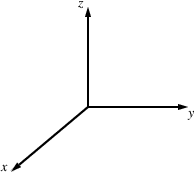
\includegraphics{9_1_right_hand_system}}
  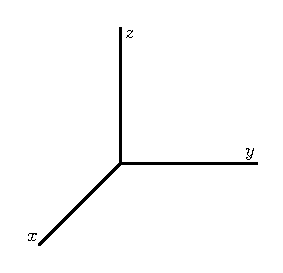
\includegraphics{figures/fig_9_1_right_hand.eps}
\caption{A right hand system}
\label{F:9.1.right_hand}
\end{center}
\end{minipage}
\hspace{0.5in}
\begin{minipage}{2.5in}
\begin{center}
%\resizebox{!}{1.5in}{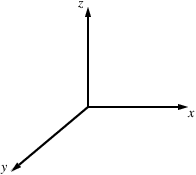
\includegraphics{9_1_left_hand_system}}
  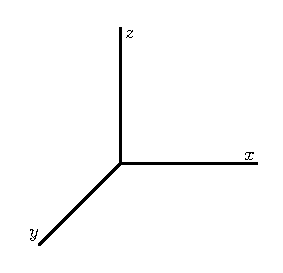
\includegraphics{figures/fig_9_1_left_hand.eps}
\caption{A left hand system}
\label{F:9.1.left_hand}
\end{center}
\end{minipage}
\end{center}
\end{figure}

The distinction between these two figures is subtle, but important.
In the coordinate system shown in \ref{F:9.1.right_hand}, imagine that
you are sitting on the positive $z$-axis next to the label ``$z$.''
Looking down at the $x$- and $y$-axes, you see that the $y$-axis is
obtained by rotating the $x$-axis by 90$^\circ$ in the {\em
  counterclockwise} direction.  Again sitting on the positive $z$-axis
in Figure \ref{F:9.1.left_hand}, you see that the $y$-axis is obtained
by rotating the $x$-axis by 90$^\circ$ in the {\em clockwise}
direction.


We call the coordinate system in \ref{F:9.1.right_hand} a {\em
  right-hand system}; if we point the index finger of our {\em right}
hand along the positive $x$-axis and our middle finger along the
positive $y$-axis, then our thumb points in the direction of the
positive $z$-axis.  Following mathematical conventions, we choose to
use a right-hand system throughout this book.

% We will adopt a right-hand system\index{right hand system}, as illustrated in Figure \ref{F:9.1.right_hand}. To see the difference, think about a socket wrench -- a tool for driving screws. It consists of a handle and a socket. The socket is placed on the screw and attached to the handle. As the handle of the wrench is turned, the socket provides a force that drives the screw. If you point the index finger of your right hand in the direction of the force you apply to the handle of the wrench, and point your middle finger in the direction of the handle toward the socket, then your thumb will point in the direction in which the wrench is driving the screw. If you use your left hand instead, then your thumb will point in the opposite direction. So the socket wrench is set up to drive right-handed screws. This is exactly the 3D coordinate system we want to adopt. In a right hand system, if we point the index finger of our right hand in the direction of the positive $x$-axis and our middle finger in the direction of the positive $y$-axis, then our thumb will point in the direction of the positive $z$-axis. A left hand system and a right hand system have different orientations, so we need pick one as a standard so that the convention of orientation is understood by everyone. We will always use a right-hand system.

Now that we have established a convention for a right hand system, we can draw a graph of the range function, $f(x,y) = \frac{x^2 \sin(2y)}{g}$. Note that the function $f$ is continuous in both variables, so when we plot these points in the right hand coordinate system, we can connect them all to form a surface in 3-space. The graph of the range function $f$ is shown in Figure \ref{F:9.1.range}.
\begin{figure}[ht]
\begin{center}
%\resizebox{!}{2.0in}{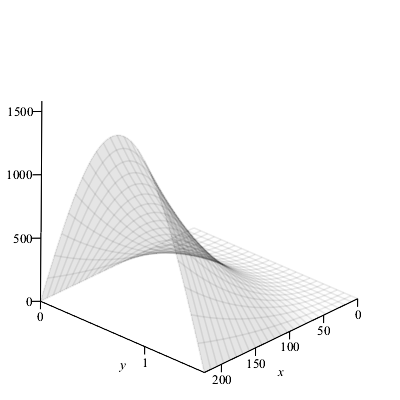
\includegraphics[trim=0cm 0cm 1cm 4.5cm,
%clip]{9_1_range}}
  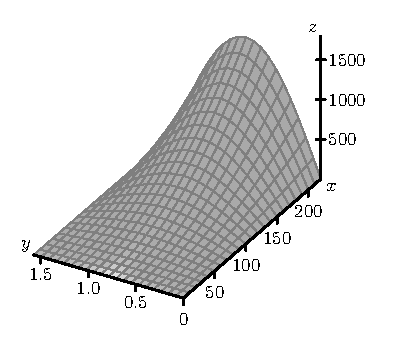
\includegraphics{figures/fig_9_1_range.eps}
\caption{The range surface.}
\label{F:9.1.range}
\end{center}
\end{figure}
%trim=left bottom right top, need clip

There are many graphing tools available for drawing three-dimensional
surfaces.\footnote{e.g., Wolfram Alpha and
  \url{http://web.monroecc.edu/manila/webfiles/calcNSF/JavaCode/CalcPlot3D.htm}}
Since we will be able to visualize graphs of functions of two
variables, but not functions of more than two variables, we will
primarily deal with functions of two variables in this course. It is
important to note, however, that the techniques we develop apply to
functions of any number of variables.
%We will work extensively with functions of several variables in subsequent sections.

\vspace{10pt}

\noindent \textbf{Notation:} We let $\R^2$ denote the set of all
ordered pairs of real numbers in the plane (two copies of the real
number system) and let $\R^3$ represent the set of all ordered triples
of real numbers (which constitutes three-space).

\vspace{10pt}

\subsection*{Some Standard Equations in Three-Space}

In addition to graphing functions, we will also want to understand
graphs of some simple equations in three dimensions. For example, in
$\R^2$, the graphs of the equations $x=a$ and $y=b$, where $a$ and $b$
are constants, are lines parallel to the coordinate axes. In the next
activity we consider their three-dimensional analogs.

\begin{activity} \label{A:9.1.3}
    \ba
    \item Consider the set of points $(x,y,z)$ that satisfy the equation $x=2$. Describe this set as best you can.

    \item Consider the set of points $(x,y,z)$ that satisfy the equation $y=-1$. Describe this set as best you can.


    \item Consider the set of points $(x,y,z)$ that satisfy the equation $z=0$. Describe this set as best you can.


    \ea
\end{activity}
\begin{smallhint}
\ba
\item What does the set of points $(0,y,z)$ look like? 
\item What does the set of points $(x,0,z)$ look like?
\item What does the set of points $(x,y,0)$ look like?
\ea
\end{smallhint}
\begin{bighint}
\ba
\item What does the set of points $(0,y,z)$ look like? 
\item What does the set of points $(x,0,z)$ look like?
\item What does the set of points $(x,y,0)$ look like?
\ea
\end{bighint}
\begin{activitySolution}
\ba
\item If we let only $y$ and $z$ vary, the result will be a plane. If $x$ is fixed at $2$, the resulting plane will be parallel to the $yz$-plane and a distance 2 in front of the $yz$-plane (in the positive $x$-direction).   
\item If we let only $x$ and $z$ vary, the result will be a plane. If $y$ is fixed at $-1$, the resulting plane will be parallel to the $xz$-plane and a distance 1 to the left of the $xz$-plane (in the negative $y$-direction). 
\item If we let only $x$ and $y$ vary, the result will be a plane. If $z$ is fixed at $0$, the resulting plane will be just the $xy$-plane. 
\ea
\end{activitySolution}
\aftera 

Activity \ref{A:9.1.3} shows that the equations where one independent
variable is constant lead to planes parallel to ones that result from
a pair of the coordinate axes. When we make the constant 0, we get the
\emph{coordinate planes}\index{coordinate planes}. The $xy$-plane
satisfies $z=0$, the $xz$-plane satisfies $y=0$, and the $yz$-plane
satisfies $z=0$ (see Figure \ref{F:9.1.coordinate_planes}).

\begin{figure}[ht]
\begin{center}
%\resizebox{!}{1.25in}{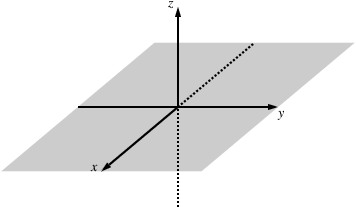
\includegraphics{9_1_xy_plane}}
  
\includegraphics{figures/fig_9_1_xy_plane.eps}
\hspace{0.2in}
%\resizebox{!}{1.25in}{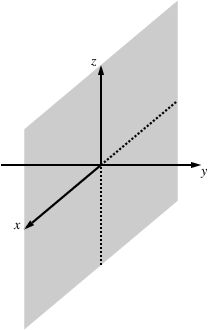
\includegraphics{9_1_xz_plane}}
  
\includegraphics{figures/fig_9_1_xz_plane.eps}
\hspace{0.3in}
%\resizebox{!}{1.25in}{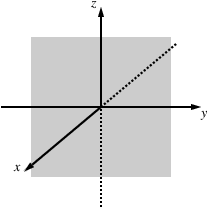
\includegraphics{9_1_yz_plane}}
  
\includegraphics{figures/fig_9_1_yz_plane.eps}
\end{center}
\caption{The coordinate planes.}
\label{F:9.1.coordinate_planes}
\end{figure}

On a related note, we define a circle in $\R^2$ as the set of all
points equidistant from a fixed point. In $\R^3$, we call the set of
all points equidistant from a fixed point a
\emph{sphere}\index{sphere!definition}. To find the equation of a
sphere, we need to understand how to calculate the distance between
two points in three-space, and we explore this idea in the next
activity.

\begin{activity} \label{A:9.1.4}
    Let $P=(x_0, y_0, z_0)$ and $Q=(x_1, y_1, z_1)$ be two points in $\R^3$. These two points form opposite vertices of a rectangular box whose sides are planes parallel to the coordinate planes as illustrated in Figure \ref{F:9.1.Distance_3D}, and the distance between $P$ and $Q$ is the length of the diagonal shown in Figure \ref{F:9.1.Distance_3D}.
    \begin{figure}[ht]
\begin{center}
%\resizebox{!}{2.0in}{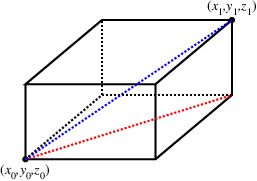
\includegraphics{figures/9_1_Distance_3D}}
  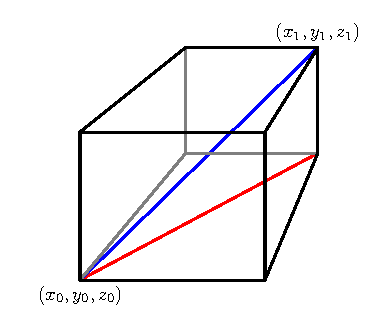
\includegraphics{figures/fig_9_1_distance.eps}
\caption{The distance formula in $\R^3$.}
\label{F:9.1.Distance_3D}
\end{center}
\end{figure}
    \ba
  \item Consider one of the right triangles in the base of the box whose
    hypotenuse is shown as the red line in Figure
    \ref{F:9.1.Distance_3D}. What are the vertices of this triangle?
    Since this right triangle lies in a plane, we can use the
    Pythagorean Theorem to find a formula for the length of the
    hypotenuse of this triangle. Find such a formula, which will be in
    terms of $x_0$, $y_0$, $x_1$, and $y_1$.

  \item Now notice that the triangle whose hypotenuse is the blue segment
    connecting the points $P$ and $Q$ with a leg as the hypotenuse of
    the triangle found in part (a) lies entirely in a plane, so we can
    again use the Pythagorean Theorem to find the length of its
    hypotenuse. Explain why the length of this hypotenuse, which is
    the distance between the points $P$ and $Q$, is
        \begin{equation*} %\label{eq:9.1.Distance_3D}
        \sqrt{(x_1-x_0)^2 + (y_1-y_0)^2 + (z_1-z_0)^2}.
        \end{equation*}

    \ea
\end{activity}
\begin{smallhint}
\ba
\item What are the equations of the faces of the box?
\item What is the distance between the point $Q$ and the point at the lower right corner of the back of the box? 
\ea

\end{smallhint}
\begin{bighint}
\ba
\item The front face of the box has equation $x=x_0$ and the right face of the box has equation $y=y_1$. 
\item What is the distance between the point $Q$ and the point at the lower right corner of the back of the box? 
\ea
\end{bighint}
\begin{activitySolution}
\ba
\item The front face of the box is the $x=x_0$ plane, the back is the $x=x_1$ plane, the bottom is the $z=z_0$ plane, and the right side is the $y=y_1$ plane. So the coordinates of the point at the lower front right of the box are $(x_0,y_1,z_0)$ and the coordinates of the point at the back lower right of the box are $(x_1, y_1, z_0)$. The length of the legs of this triangle are $\mid y_1-y_0\mid$  (the distance between the points $(x_0, y_0, z_0)$ and $(x_0,y_1,z_0)$) and $\mid x_1-x_0 \mid$ (the distance between the points $(x_0, y_1, z_0)$ and $(x_1,y_1,z_0)$). The Pythagorean Theorem then shows that the length of the hypotenuse of the triangle in the base of the box is  
\[\sqrt{(x_1-x_0)^2+(y_1-y_0)^2}.\]
\item The distance between $P$ and $Q$ is the length of the hypotenuse of the triangle whose legs are the hypotenuse of the triangle in the base of the box and whose height is the distance between the points $Q=(x_1,y_1,z_1)$ and $R=(x_1, y_1, z_0)$ (the point at the bottom right corner of the back of the box). The distance between $Q$ and $R$ is just $\mid z_1-z_0\mid$. Using the result from part (a), the Pythagorean Theorem shows that the distance between $P$ and $Q$ is 
\[\sqrt{\left(\sqrt{(x_1-x_0)^2+(y_1-y_0)^2}\right)^2 + (z_1-z_0)^2} = \sqrt{(x_1-x_0)^2 + (y_1-y_0)^2 + (z_1-z_0)^2}\]
as desired.  
\ea
\end{activitySolution}
\aftera 


The formula developed in Activity \ref{A:9.1.4} is important to remember.

\vspace*{5pt}
\nin \framebox{\hspace*{3 pt}
\parbox{6.25 in}{The distance between points $P=(x_0, y_0, z_0)$ and $Q=(x_1, y_1, z_1)$ (denoted as $|PQ|$)  in $\R^3$ is given by the formula
\begin{equation} \label{eq:9.1.Distance_3D}
|PQ| = \sqrt{(x_1-x_0)^2 + (y_1-y_0)^2 + (z_1-z_0)^2}.
\end{equation}
} \hspace*{3 pt}}
\vspace*{5pt}

Equation (\ref{eq:9.1.Distance_3D}) can be used to derive the formula
for a sphere\index{sphere!formula} centered at a point $(x_0,y_0,z_0)$
with radius $r$. Since the distance from any point $(x,y,z)$ on such a
sphere to the point $(x_0,y_0,z_0)$ is $r$, the point $(x,y,z)$ will
satisfy the equation
\[\sqrt{(x-x_0)^2 + (y-y_0)^2 + (z-z_0)^2} = r\]
%or
%\[(x-x_0)^2 + (y-y_0)^2 + (z-z_0)^2 = r^2.\]
Squaring both sides, we come to the standard equation for a sphere.

\vspace*{5pt}
\nin \framebox{\hspace*{3 pt}
\parbox{6.25 in}{The equation of a sphere with center $(x_0,y_0,z_0)$ and radius $r$ is
\[(x-x_0)^2 + (y-y_0)^2 + (z-z_0)^2 = r^2.\]
} \hspace*{3 pt}}
\vspace*{5pt}

This makes sense if we compare this equation to its two-dimensional
analogue, the equation of a circle of radius $r$ in the plane centered
at $(x_0,y_0)$:
$$
(x-x_0)^2 + (y-y_0)^2 = r^2.
$$


%\begin{activity} \label{A:9.1.5}
    Find the equation of the sphere centered at the point $(2,1,3)$ if the point $(-1,0,-1)$ lies on the sphere.

\end{activity}
\begin{smallhint}

\end{smallhint}
\begin{bighint}

\end{bighint}
\begin{activitySolution}

\end{activitySolution}
\aftera 

\subsection*{Traces}

When we study functions of several variables we are often interested
in how each individual variable affects the function in and of
itself. In Preview Activity \ref{PA:9.1}, we saw that the monthly
payment on an \$18,000 loan depends on the interest rate and the
duration of the loan. However, if we fix the interest rate, the
monthly payment depends only on the duration of the loan, and if we
set the duration the payment depends only on the interest rate. This
idea of keeping one variable constant while we allow the other to
change will be an important tool for us when studying functions of
several variables.

As another example, consider again the range function $f$ defined by
\[f(x,y) = \frac{x^2 \sin(2y)}{g}\] where $x$ is the initial velocity
of an object in feet per second, $y$ is the launch angle in radians,
and $g$ is the acceleration due to gravity (32 feet per second
squared). If we hold the launch angle constant at $y=0.6$ radians, we
can consider $f$ a function of the initial velocity alone. In this
case we have
\[f(x) = \frac{x^2}{32}\sin(2\cdot 0.6).\]
We can plot this curve on the surface by tracing out the points on the
surface when $y = 0.6$, as shown in Figure
\ref{F:9.1.trace1}. The graph and the formula clearly show that $f$ is
quadratic in the $x$-direction. More descriptively, as we increase the
launch velocity while keeping the launch angle constant, the range
increases proportional to the square of the initial velocity.

Similarly, if we fix the initial velocity at 150 feet per second, we
can consider the range as a function of the launch angle only. In this
case we have
\[f(y) = \frac{150^2 \sin(2y)}{32}.\] 
We can again plot this curve on
the surface by tracing out the points on the surface when $x=150$, as
shown in Figure \ref{F:9.1.trace2}. The graph and the formula clearly
show that $f$ is sinusoidal in the $y$-direction. More descriptively,
as we increase the launch angle while keeping the initial velocity
constant, the range is proportional to the sine of twice the launch
angle.
\begin{figure}[ht]
\begin{center}
\begin{minipage}{2.5in}
\begin{center}
%\resizebox{!}{1.75in}{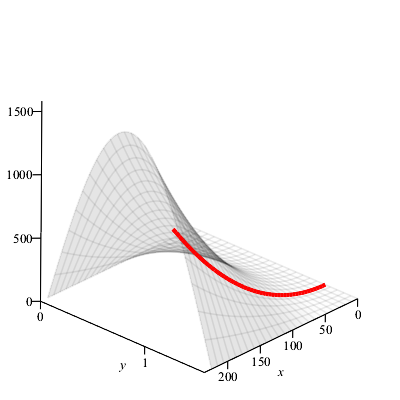
\includegraphics[trim=0cm 0cm 1cm 4.5cm,
%clip]{9_1_trace1}}
  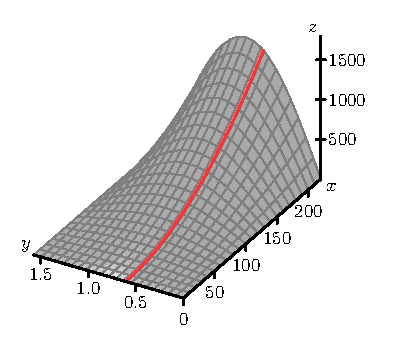
\includegraphics{figures/fig_9_1_y_range.eps}
\caption{The trace with $y = 0.6$.}
\label{F:9.1.trace1}
\end{center}
\end{minipage}
\hspace{0.5in}
\begin{minipage}{2.5in}
\begin{center}
%\resizebox{!}{1.75in}{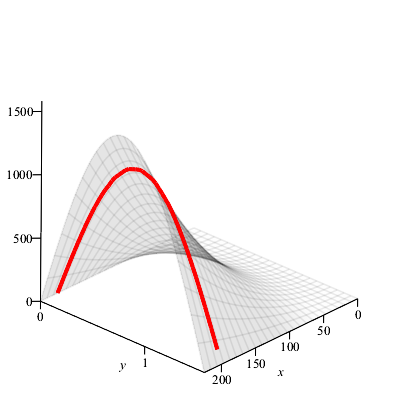
\includegraphics[trim=0cm 0cm 1cm 4.5cm, clip]{9_1_trace2}}
  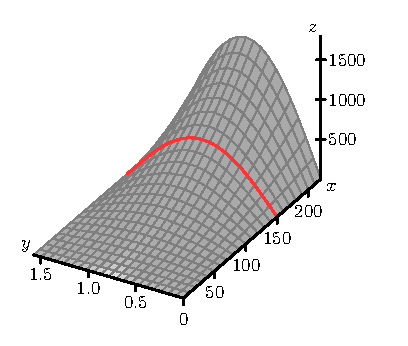
\includegraphics{figures/fig_9_1_x_range.eps}
\caption{The trace with $x = 150$.}
\label{F:9.1.trace2}
\end{center}
\end{minipage}
\end{center}
\end{figure}

The curves we define when we fix one of the independent variables in our two variable function are called \emph{traces}.

\vspace*{5pt}
\nin \framebox{\hspace*{3 pt}
\parbox{6.25 in}{\begin{definition} A \textbf{trace}\index{trace} of a function $f$ of two independent variables $x$ and $y$ is a curve of the form $z = f(c,y)$ or $z = f(x,c)$, where $c$ is a constant. \end{definition}
} \hspace*{3 pt}}
\vspace*{5pt}

Understanding trends in the behavior of functions of two variables can
be challenging, as can sketching their graphs; traces help us with
each of these tasks.

\begin{activity} \label{A:9.1.6}
    In the following questions, we investigate the use of traces to better understand a function through both tables and graphs.  
    \ba
  \item Identify the $y = 0.6$ trace for the range function $f(x,y) =
    \frac{x^2 \sin(2y)}{g}$ by highlighting or circling the
    appropriate cells in Table \ref{T:9.1.range}.  Write a sentence to
    describe the behavior of the function along this trace.

  \item Identify the $x = 150$ trace for the range function by
    highlighting or circling the appropriate cells in Table
    \ref{T:9.1.range}.  Write a sentence to describe the behavior of
    the function along this trace.

 \begin{figure}[ht]
\begin{center}
%\resizebox{!}{2.0in}{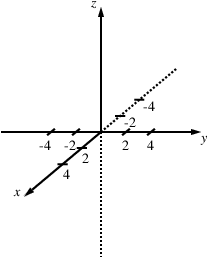
\includegraphics{figures/9_1_traces_activity_1}}
  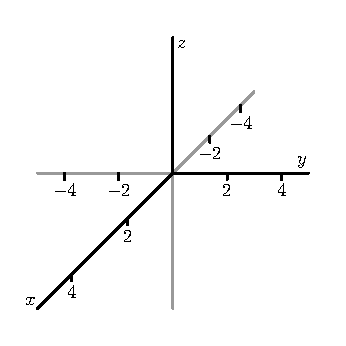
\includegraphics{figures/fig_9_1_activity_axes.eps}
\caption{Coordinate axes to sketch traces.}
\label{F:9.1.traces_activity_1}
\end{center}
\end{figure}

   \item For the function $g(x,y) = x^2 + y^2 + 1$, explain the type of function that each trace in the $x$ direction will be (keeping $y$ constant). Plot the $y=-4$, $y=-2$, $y=0$, $y=2$, and $y=4$ traces in 3-dimensional coordinate system provided in Figure \ref{F:9.1.traces_activity_1}.

    \item For the function $g(x,y) = x^2 + y^2 + 1$, explain the type of function that each trace in the $y$ direction will be (keeping $x$ constant). Plot the $x=-4$, $x=-2$, $x=0$, $x=2$, and $x=4$ traces in 3-dimensional coordinate system in Figure \ref{F:9.1.traces_activity_1}.

    \item Describe the surface generated by the function $g$.

     \ea



\end{activity}
\begin{smallhint}
\ba
\item Do the $y$ values run down the columns or across the rows?
\item Do the $x$ values run down the columns or across the rows?
\item If $y$ is constant, the only variables are $x$ and $z$. 
\item If $x$ is constant, the only variables are $y$ and $z$.
\item What do the traces look like?
\ea 
\end{smallhint}
\begin{bighint}
\ba
\item Do the $y$ values run down the columns or across the rows?
\item Do the $x$ values run down the columns or across the rows?
\item What does the graph of $z=x^2+C$ look like if $C$ is a constant?
\item What does the graph of $z=y^2+C$ look like if $C$ is a constant?
\item What do the traces look like?
\ea
\end{bighint}
\begin{activitySolution}
\ba
\item The $y$ values in the table are those that run across the rows. So fixing $y$ at $\frac{2\pi}{5} = \frac{8\pi}{20}$ and letting $x$ vary amounts to looking at the $\frac{8\pi}{20}$ column in the table. The $y=\frac{2\pi}{5}$ trace is highlighted in red in the table below. This trace shows that as we increase the initial velocity $x$ while keeping the launch angle constant at $\frac{2\pi}{5}$ radians, the range of the object increases at an increasing rate. 
\begin{center}
\begin{tabular}{|c|c|c|c|c|c|c|c|>{\columncolor{tracered}}c|c|c|} \hline
  &$\frac{\pi}{20}$ &$\frac{2\pi}{20}$ &$\frac{3\pi}{20}$ &$\frac{4\pi}{20}$ &$\frac{5\pi}{20}$ &$\frac{6\pi}{20}$ &$\frac{7\pi}{20}$ &$\frac{8\pi}{20}$ &$\frac{9\pi}{20}$    &$\frac{\pi}{2}$ \\ \hline
25      &6.036      &11.480     &15.801     &18.575     &19.531     &18.575     &15.801     &11.480     &6.0356     &0.000 \\ \hline
50      &24.142     &45.921     &63.205     &74.301     &78.125     &74.301     &63.205     &45.921     &24.142     &0.000 \\ \hline
75      &54.319     &103.322    &142.210    &167.178    &175.781    &167.178    &142.210    &103.322    &54.319     &0.000 \\ \hline
100     &96.568     &183.683    &252.818    &297.205    &312.500    &297.205    &252.818    &183.683    &96.568     &0.000 \\ \hline
125     &150.887    &287.005    &395.028    &464.383    &488.281    &464.383    &395.028    &287.005    &150.887    &0.000 \\ \hline
150     &217.278    &413.287    &568.840    &668.712    &703.125    &668.712    &568.840    &413.287    &217.278    &0.000 \\ \hline
175     &295.739    &562.529    &774.255    &910.191    &957.031    &910.191    &774.255    &562.529    &295.739    &0.000 \\ \hline
200     &386.271    &734.732    &1011.271   &1188.821   &1250.000   &1188.821   &1011.271   &734.732    &386.271    &0.000 \\ \hline
225     &488.875    &929.895    &1279.890   &1504.601   &1582.031   &1504.601   &1279.890   &929.895    &488.875    &0.000 \\ \hline
250     &603.549    &1148.018   &1580.112   &1857.532   &1953.125   &1857.532   &1580.112   &1148.018   &603.549    &0.000 \\ \hline
\end{tabular}
\end{center}
\item  The $x$ values in the table are those that run down the columns. So fixing $x$ at $150$ and letting $y$ vary amounts to looking at the $150$ row in the table. The $x=150$ trace is highlighted in blue in the table below. This trace shows that as we increase the launch angle $y$ while keeping the initial velocity $x$ at a constant $150$ feet per second, the range increases at first until we reach an angle of approximately $\frac{pi}{4}$, and then decreases. 
%\begin{table}[ht]
\begin{center}
\begin{tabular}{|c|c|c|c|c|c|c|c|c|c|c|} \hline
  &$\frac{\pi}{20}$ &$\frac{2\pi}{10}$ &$\frac{3\pi}{20}$ &$\frac{4\pi}{20}$ &$\frac{5\pi}{20}$ &$\frac{6\pi}{20}$ &$\frac{7\pi}{20}$ &$\frac{8\pi}{20}$ &$\frac{9\pi}{20}$    &$\frac{\pi}{2}$ \\ \hline
25      &6.036      &11.480     &15.801     &18.575     &19.531     &18.575     &15.801     &11.480     &6.0356     &0.000 \\ \hline
50      &24.142     &45.921     &63.205     &74.301     &78.125     &74.301     &63.205     &45.921     &24.142     &0.000 \\ \hline
75      &54.319     &103.322    &142.210    &167.178    &175.781    &167.178    &142.210    &103.322    &54.319     &0.000 \\ \hline
100     &96.568     &183.683    &252.818    &297.205    &312.500    &297.205    &252.818    &183.683    &96.568     &0.000 \\ \hline
125     &150.887    &287.005    &395.028    &464.383    &488.281    &464.383    &395.028    &287.005    &150.887    &0.000 \\ \hline
150     &217.278    &413.287    &568.840    &668.712    &703.125    &668.712    &568.840    &413.287    &217.278    &0.000 \\ \hline
175     &295.739    &562.529    &774.255    &910.191    &957.031    &910.191    &774.255    &562.529    &295.739    &0.000 \\ \hline
\rowcolor{traceblue}
200     &386.271    &734.732    &1011.271   &1188.821   &1250.000   &1188.821   &1011.271   &734.732    &386.271    &0.000 \\ \hline
225     &488.875    &929.895    &1279.890   &1504.601   &1582.031   &1504.601   &1279.890   &929.895    &488.875    &0.000 \\ \hline
250     &603.549    &1148.018   &1580.112   &1857.532   &1953.125   &1857.532   &1580.112   &1148.018   &603.549    &0.000 \\ \hline
\end{tabular}
%\caption{Values of $f(x,y) = \frac{x^2 \sin(2y)}{g}$.}
%\label{T:tracey_sol}
\end{center}
%\end{table}
\item The portion of the surface $g$ where $y$ is constant at a value $k$ has the form 
\[g(x,k) = x^2+k^2+1.\]
This is a quadratic parallel to the $xz$-plane with its vertex at the point $(0,k,k^2+1)$, opening in the positive $z$ direction. The indicated traces are shown here %in Figure \ref{F:9.1_Act_6_1}
%\begin{figure}[ht]
\begin{center}
\resizebox{!}{2.0in}{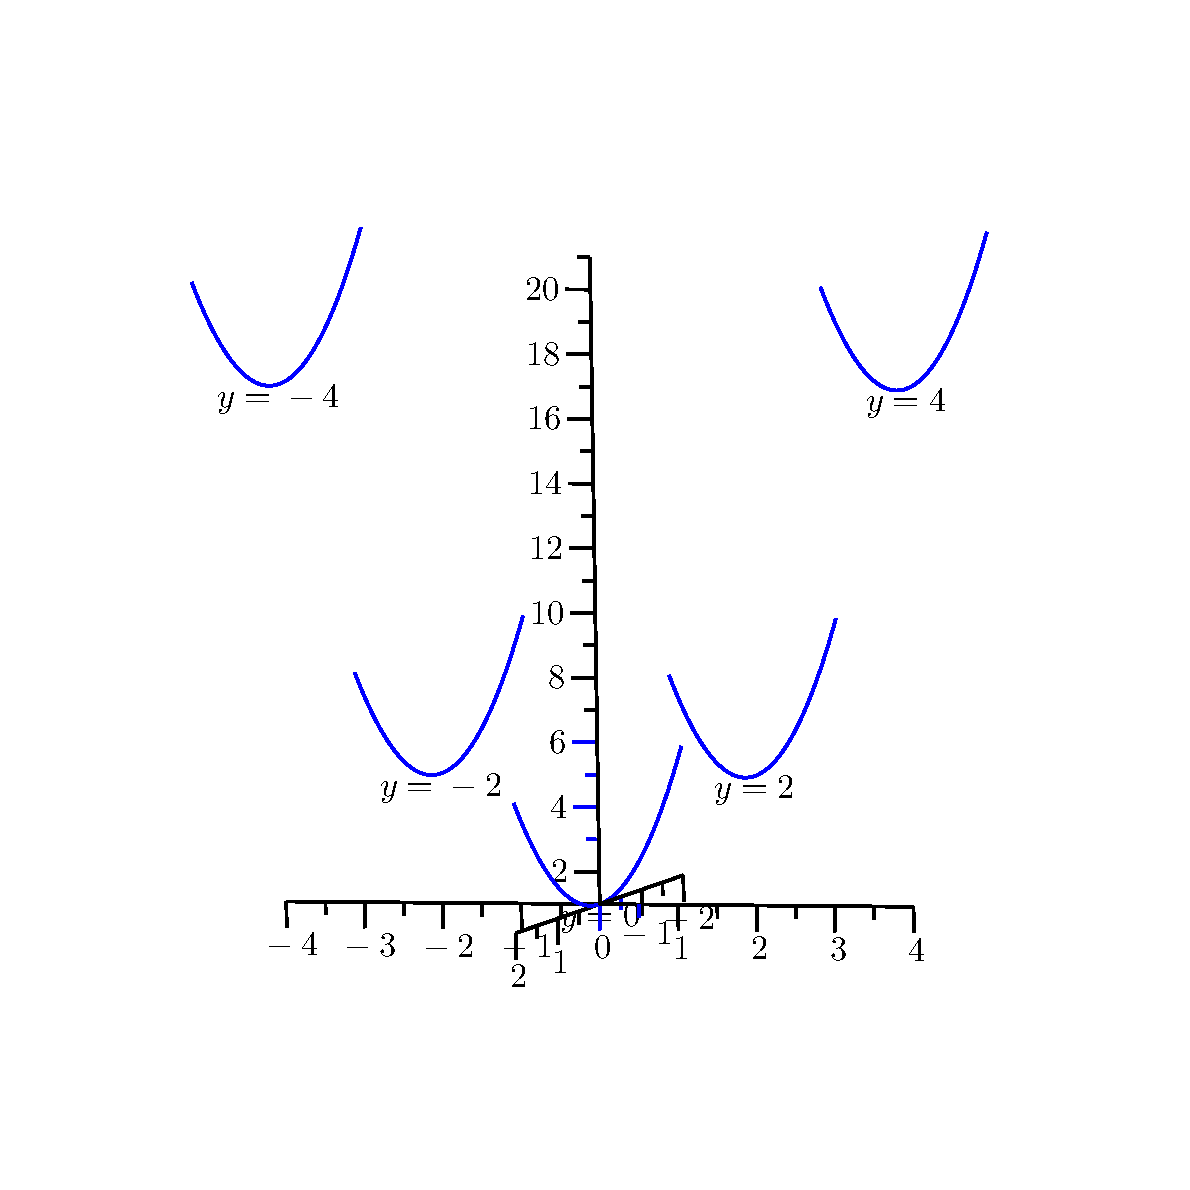
\includegraphics{figures/9_1_Act_6_1}}
%\caption{Traces in the $x$ direction.}
%\label{F:9.1_Act_6_1}
\end{center}
%\end{figure}
 \item The portion of the surface $g$ where $x$ is constant at a value $c$ has the form 
\[g(c,y) = c^2+y^2+1.\]
This is a quadratic parallel to the $yz$-plane with its vertex at the point $(c,0,c^2+1)$, opening in the positive $z$ direction. The indicated traces are shown here %in Figure \ref{F:9.1_Act_6_2}
%\begin{figure}[ht]
\begin{center}
\resizebox{!}{2.0in}{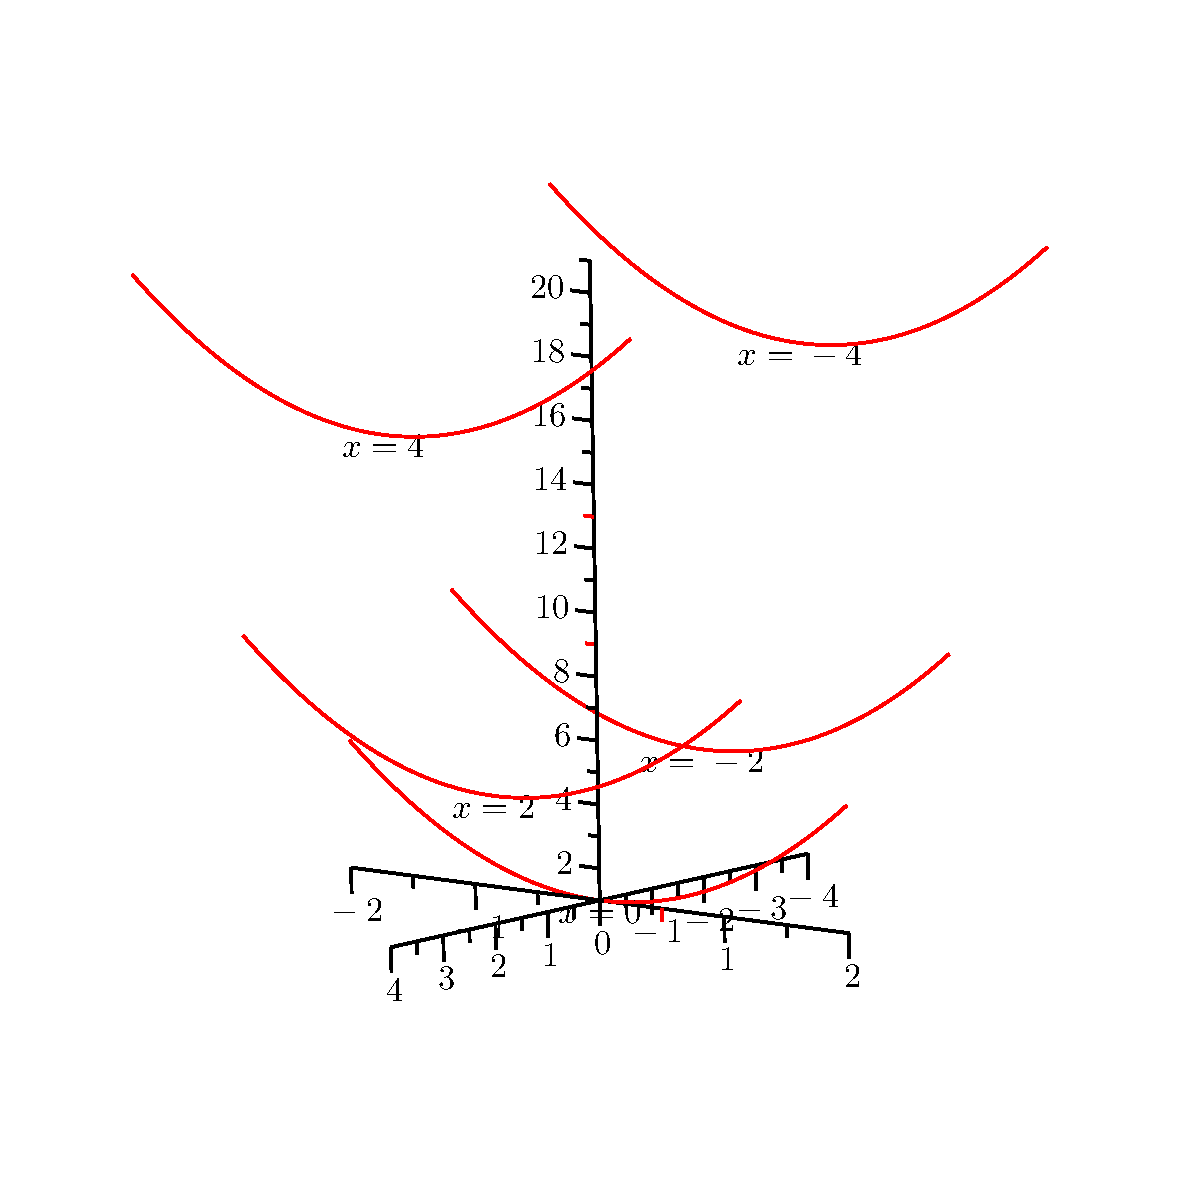
\includegraphics{figures/9_1_Act_6_2}}
%\caption{Traces in the $y$ direction.}
%\label{F:9.1_Act_6_2}
\end{center}
%\end{figure}
\item The traces of $g$ in both directions are parabolas opening in the positive $z$ direction. So the graph of $g$ should look like a bowl with its vertex at the origin, opening in the positive $z$ direction. 
\ea
\end{activitySolution}
\aftera 

%\input{activities/9.1.Act7}

\subsection*{Contour Maps and Level Curves}

We have all seen topographic maps such as the one of the Porcupine
Mountains in the upper peninsula of Michigan shown in Figure
\ref{F:9.1.porcupine}.\footnote{Map source: Michigan Department of
  Natural Resources,
  \url{https://www.michigan.gov/dnr/0,4570,7-153-10369_46675_58093---,00.html},
  with permission of the Michigan DNR and Bob Wild.} The curves on
these maps show the regions of constant altitude. The contours also
depict changes in altitude: contours that are close together signify
steep ascents or descents, while contours that are far apart indicate
only slight changes in elevation.  Thus, contour maps tell us a lot
about three-dimensional surfaces. Mathematically, if $f(x,y)$
represents the altitude at the point $(x,y)$, then each contour is the
graph of an equation of the form $f(x,y) = k$, for some constant $k$.

\newpage
\begin{landscape}
\begin{figure}[h]
\begin{center}
\resizebox{!}{5.0in}
{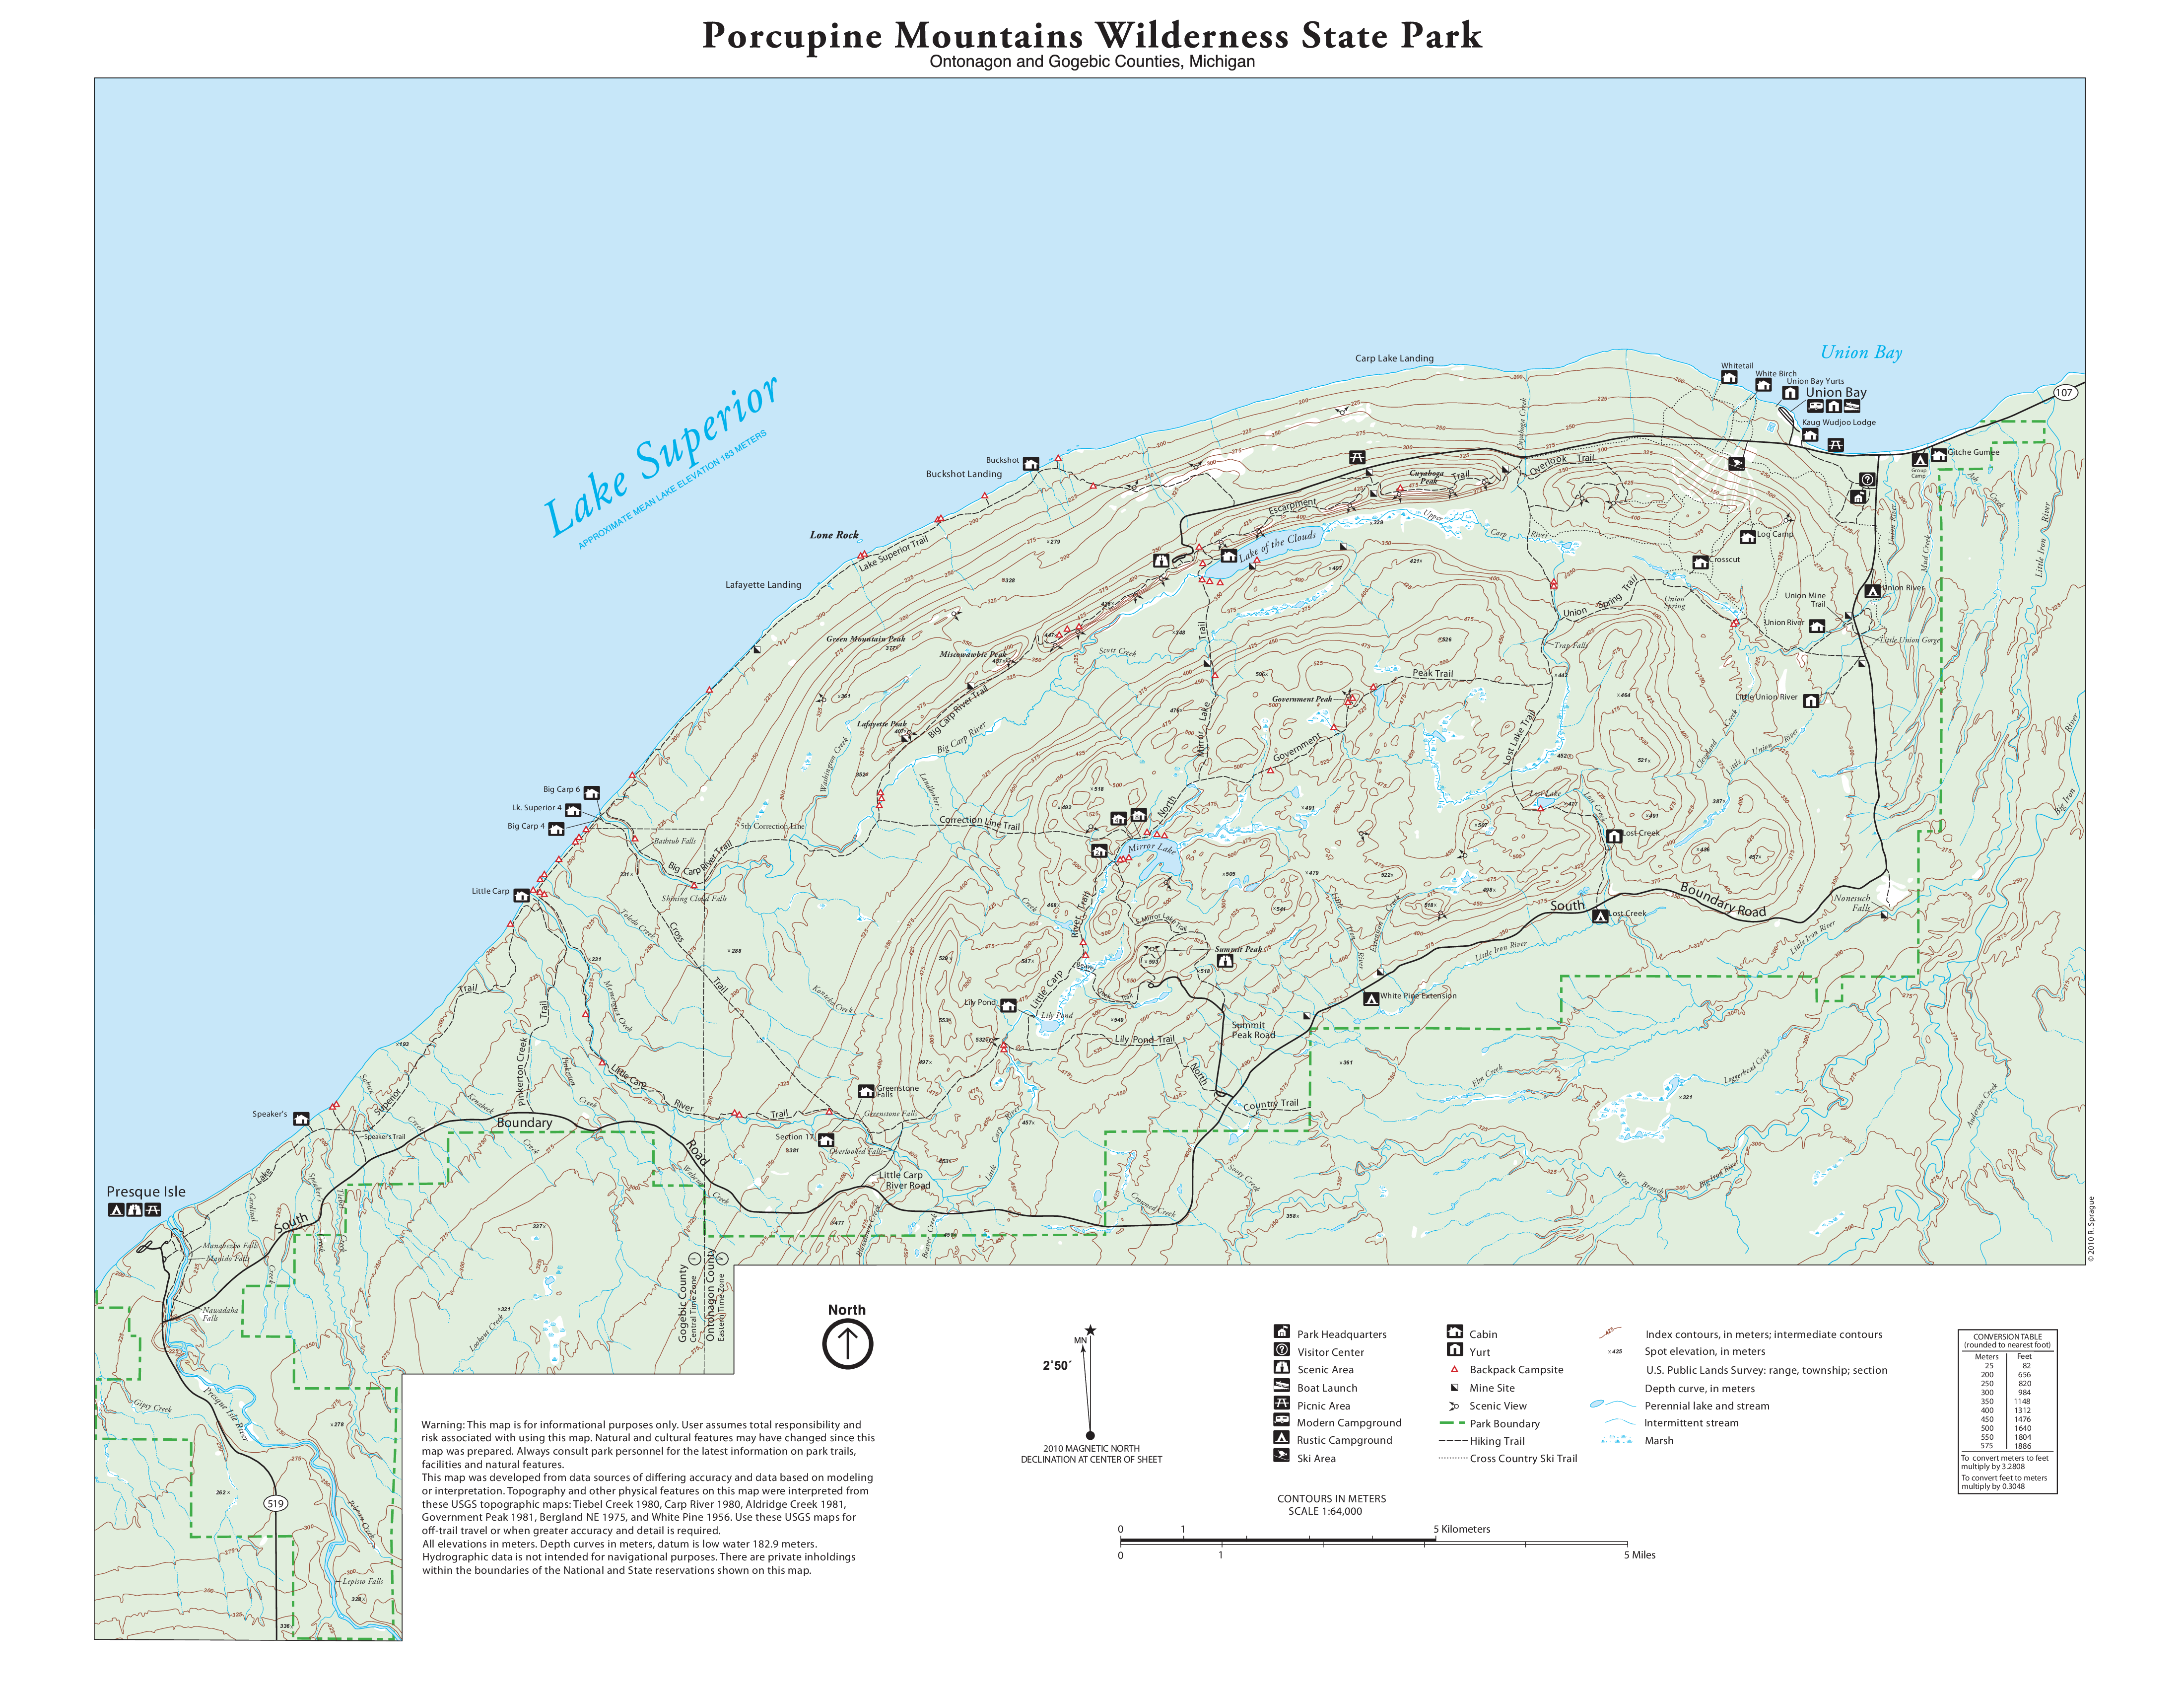
\includegraphics[trim=55cm 40cm 40cm 40cm, clip]{9_1_porcupine_2}}
%trim=left bottom right top, need clip if not animation
% 
\caption{Contour map of the Porcupine Mountains.}
\label{F:9.1.porcupine}
\end{center}
\end{figure}
\end{landscape}
\newpage

\begin{activity} \label{A:9.1.8}
   On the topographical map of the Porcupine Mountains in Figure \ref{F:9.1.porcupine},

   \ba
    \item identify the highest and lowest points you can find;
    \item from a point of your choice, determine a path of steepest ascent that leads to the highest point;
    \item from that same initial point, determine the least steep path that leads to the highest point.

     \ea

\end{activity}
\begin{smallhint}

\end{smallhint}
\begin{bighint}
\ba
\item The best you can do is search the map for the highest and lowest elevations.
\item Closely spaced contours indicate a sharp increase or decrease in elevation.
\item Widely spaced contours indicate a slow increase or decrease in elevation. 
\ea
\end{bighint}
\begin{activitySolution}
\ba
\item Summit Peak appears to be the highest point on this map at an elevation of around 593. Near the top left corner of the map there is a contour at an elevation of around 200 that seems to be the lowest on the map. 
\item The contours to the west of Summit Peak appear to be the most closely spaced, indicating the path of steepest ascent to the peak.
\item The contours to the southwest of Summit Peak appear to be the most widely spaced, indicating the path of most gentle ascent to the peak.
\ea
\end{activitySolution}

%\newpage
%\begin{landscape}
%\begin{figure}[ht]
%\begin{center}
%\resizebox{!}{4.0in}{\includegraphics[trim=40cm 40cm 40cm 40cm, clip]{figures/1_1_porcupine_2}} %trim=left bottom right top, need clip if not animation
%\caption{Contour map of the Porcupine Mountains.}
%\label{F:1.1.porcupine}
%\end{center}
%\end{figure}
%\end{landscape}
%\newpage

\aftera 

\vspace*{5pt}
\nin \framebox{\hspace*{3 pt}
\parbox{6.25 in}{\begin{definition} A \textbf{level curve\index{level curve} (or contour)} of a function $f$ of two independent variables $x$ and $y$ is a curve of the form $k = f(x,y)$, where $k$ is a constant. \end{definition}
} \hspace*{3 pt}}
\vspace*{5pt}

Topographical maps can be used to create a three-dimensional surface
from the two-dimensional contours or level curves. For example, level
curves of the range function, $f(x,y) = \frac{x^2 \sin(2y)}{32}$,
plotted in the $xy$-plane are shown in Figure
\ref{F:9.1.contours_1}. If we lift these contours and plot them at
their respective heights, then we get a picture of the surface itself,
as illustrated in Figure \ref{F:9.1.contours_2}.

\begin{figure}[ht]
\begin{center}
\begin{minipage}{2.5in}
\begin{center}
%\resizebox{!}{1.75in}{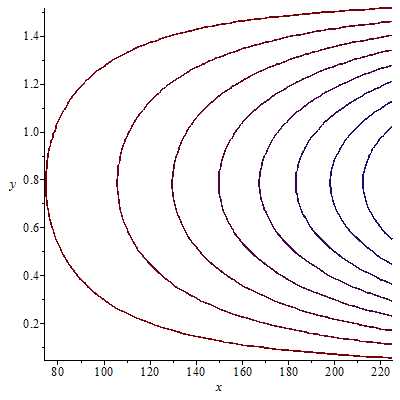
\includegraphics{9_1_contours1}}
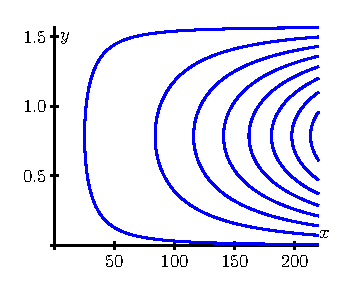
\includegraphics{figures/fig_9_1_contour_1.eps}
\caption{Several level curves.}
\label{F:9.1.contours_1}
\end{center}
\end{minipage}
\hspace{0.5in}
\begin{minipage}{2.5in}
\begin{center}
%\resizebox{!}{1.75in}{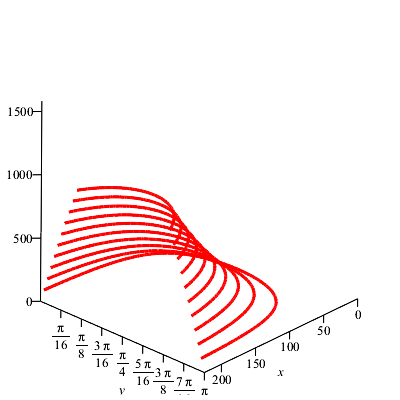
\includegraphics[trim=0cm 0cm 1cm 4.5cm, clip]{9_1_contours2}}
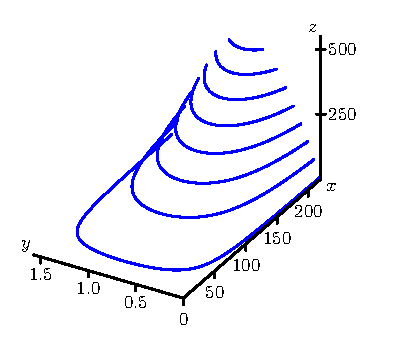
\includegraphics{figures/fig_9_1_contour_2.eps}
\caption{Level curves at the appropriate height.}
\label{F:9.1.contours_2}
\end{center}
\end{minipage}
\end{center}
\end{figure}

The use of level curves and traces can help us construct the graph of
a function of two variables.


\begin{activity} \label{A:9.1.9}
\begin{figure}[ht]
\begin{center}
%\resizebox{!}{1.75in}{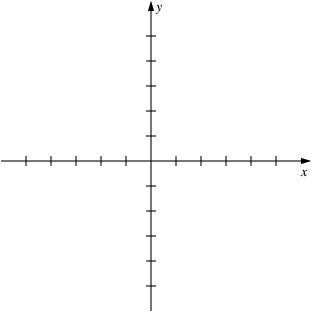
\includegraphics{figures/9_1_contour_activity_1}} 
%\hspace{0.2in} 
%\resizebox{!}{1.75in}{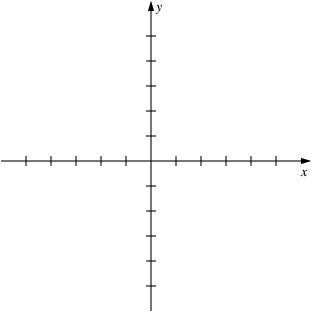
\includegraphics{figures/9_1_contour_activity_1}}
  \includegraphics{figures/fig_9_1_activity_empty_1.eps}
  \hspace*{0.5in}
  \includegraphics{figures/fig_9_1_activity_empty_2.eps}
\caption{Left: Level curves for $f(x,y) = x^2+y^2$. Right: Level curves for $g(x,y) = \sqrt{x^2+y^2}$.}
\label{F:9.1.contour_activity}
\end{center}
\end{figure}
   \ba
    \item Let $f(x,y) = x^2+y^2$. Draw the level curves $f(x,y) = k$ for $k=1$, $k=2$, $k=3$, and $k=4$ on the left set of axes given in Figure \ref{F:9.1.contour_activity}. (You decide on the scale of the axes.) Explain what the surface defined by $f$ looks like.

    \item Let $g(x,y) = \sqrt{x^2+y^2}$. Draw the level curves $g(x,y) = k$ for $k=1$, $k=2$, $k=3$, and $k=4$ on the right set of axes given in Figure \ref{F:9.1.contour_activity}. (You decide on the scale of the axes.) Explain what the surface defined by $g$ looks like.

    \item Compare and contrast the graphs of $f$ and $g$. How are they alike? How are they different? Use traces for each function to help answer these questions.

     \ea

\end{activity}
\begin{smallhint}
\ba
\item The contours have graphs that should be familiar. 
\item The contours have graphs that should be familiar.
\item How well spaced are the contours of $f$ and $g$?  
\ea
\end{smallhint}
\begin{bighint}
\ba
\item What familiar graph does the equation $x^2+y^2=1$ have?
\item What equation do you get if you square both sides of $1 = \sqrt{x^2+y^2}$?
\item What kind of graph is $y=x^2+C$ where $C$ is a constant? What kind of graph if $y = \sqrt{x^2}$? 
\ea
\end{bighint}
\begin{activitySolution}
\ba
\item The contours of $f$ are shown at left in the figure below.  The contours are circles, getting closer together as we move away from the origin, indicating a graph that is increasing quickly as we move away from the origin in all directions. The surface defined by $f$ looks like a bowl anchored at the origin that opens up. %Figure \ref{F:9.1.contour_activity_sol}.
\item The contours of $g$ are shown at right in the figure below. The contours are circles that appear to be uniformly spaced as we move away from the origin. This indicates that the surface defined by $g$ looks like a cone anchored at the origin that opens up. %Figure \ref{F:9.1.contour_activity_sol}. 
    \item The contours of $g$ are more uniformly spaced as we move away from the origin than those  in part (a). So we should expect the graph of $f$ to increase more rapidly as we move radially from the origin than the graph of $g$. To see this in another light, the traces of $f$ for fixed $y$ have the form $z = k^2+x^2$ for constants $k$, which are parabolic in form. By symmetry, the traces of $f$ for fixed values of $x$ have the same shape. By contrast, the traces of $g$ for fixed $y$ have the form $z = \sqrt{k^2+x^2}$ for constants $k$. In particular, the trace with $k=0$ has the form $z = \sqrt{x^2} = | x |$, which is linear. By symmetry, the traces for fixed $y$ have the same shape. This confirms our statements in (a) and (b) that the graph of $f$ is parabolic (bowl shaped), while the graph of $g$ looks like a cone. 
    \ea
%\begin{figure}[ht]
\begin{center}
\resizebox{!}{1.75in}{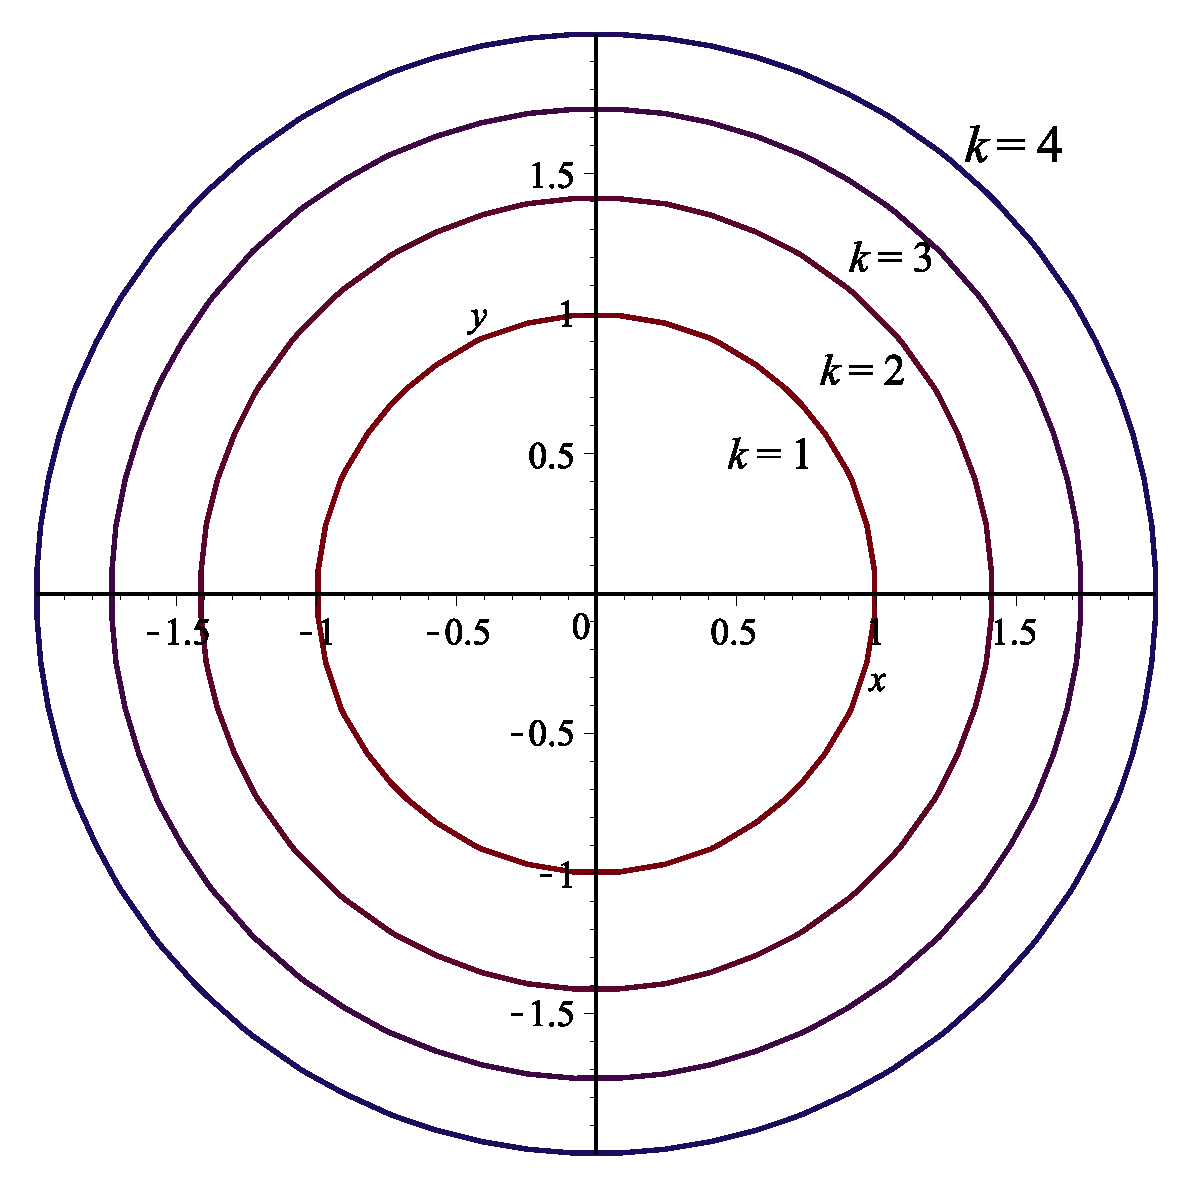
\includegraphics{figures/9_1_contour_activity_1a}} \hspace{0.2in} \resizebox{!}{1.75in}{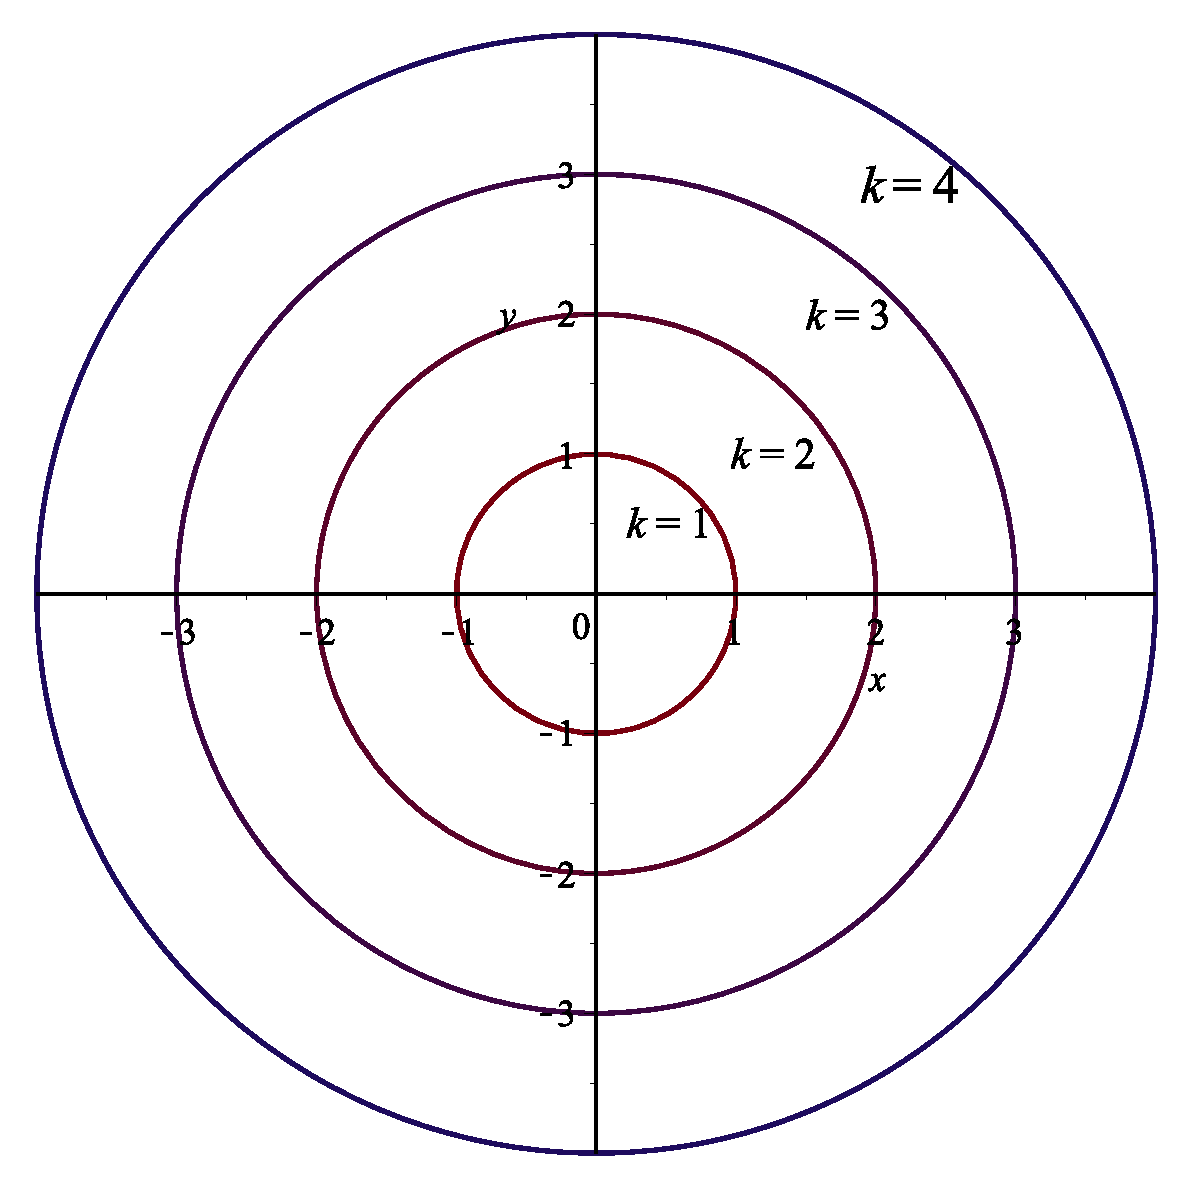
\includegraphics{figures/9_1_contour_activity_1b}}
%\caption{Left:Level curves for $f(x,y) = x^2+y^2$. Right: Level curves for $g(x,y) = \sqrt{x^2+y^2}$.}
%\label{F:9.1.contour_activity_sol}
\end{center}
%\end{figure}
\end{activitySolution}


\aftera 

%
\begin{activity} \label{A:9.1.10}
The Ideal Gas Law $PV = RT$ relates the pressure ($P$, in pascals), temperature ($T$, in Kelvin), and volume ($V$, in cubic meters) of 1 mole of a gas ($R =  8.314 \ \frac{\text{J}}{\text{mol} \ \text{K}}$ is the universal gas constant), and describes the behavior of gases that do not liquefy easily, such as oxygen and hydrogen. We can solve the ideal gas law for the volume and treat the volume as a function of the pressure and temperature:
\[V(P,T) = \frac{8.314T}{P}.\]
    \ba
    \item Explain in detail what the trace of $V$ with $P=1000$ tells us.
    \item Explain in detail what the trace of $V$ with $T=5$ tells us.
    \item Explain in detail what the level curve $V = 0.5$ tells us.
    \ea
\end{activity}
\begin{smallhint}

\end{smallhint}
\begin{bighint}

\end{bighint}
\begin{activitySolution}


\end{activitySolution}


\aftera 

The traces and level curves of a function of two variables are curves
in space. In order to understand these traces and level curves better,
we will first spend some time learning about vectors and vector-valued
functions in the next few sections and return to our study of
functions of several variables once we have those more mathematical
tools to support their study.

\subsection*{A gallery of functions}

We end this section by considering a collection of functions and
illustrating their graphs and some level curves.

\begin{figure}[ht]
  \begin{center}
    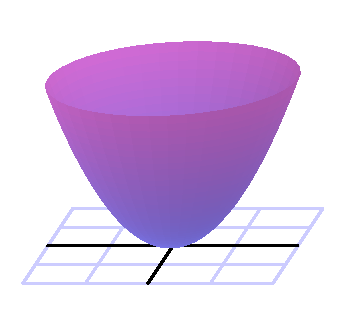
\includegraphics{figures/zisr2.eps}
    \hspace*{30pt}
    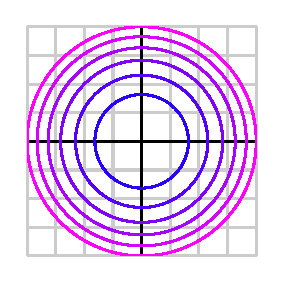
\includegraphics{figures/zisr2_contours.eps}
  \end{center}
  \caption{$z=x^2+y^2$}
\end{figure}
\begin{figure}[ht]
  \begin{center}
    
\includegraphics{figures/zis4r2.eps}
    \hspace*{30pt}
    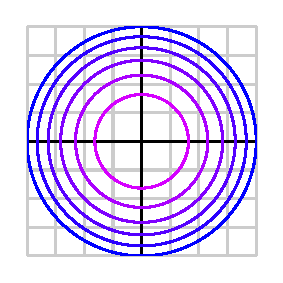
\includegraphics{figures/zis4r2_contours.eps}
  \end{center}
  \caption{$z=4-(x^2+y^2)$}
\end{figure}
\begin{figure}[ht]
  \begin{center}
    
\includegraphics{figures/cone.eps}
    \hspace*{30pt}
    
\includegraphics{figures/cone_contours.eps}
  \end{center}
  \caption{$z=\sqrt{x^2+y^2}$}
\end{figure}
\clearpage
\begin{figure}[ht]
  \begin{center}
    
\includegraphics{figures/saddle.eps}
    \hspace*{30pt}
    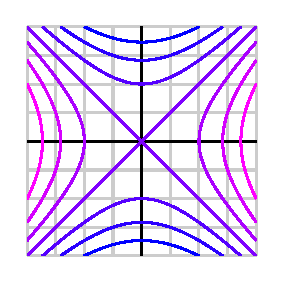
\includegraphics{figures/saddle_contours.eps}
  \end{center}
  \caption{$z=x^2-y^2$}
\end{figure}
\begin{figure}[ht]
  \begin{center}
    \includegraphics{figures/sinxy.eps}
    \hspace*{30pt}
    \includegraphics{figures/sinxy_contours.eps}
  \end{center}
  \caption{$z=\sin(x)+\sin(y)$}
\end{figure}
\clearpage
\begin{figure}[ht]
  \begin{center}
    \includegraphics{figures/elliptic.eps}
    \hspace*{30pt}
    \includegraphics{figures/elliptic_contours.eps}
  \end{center}
  \caption{$z=y^2 - x^3 + x$}
\end{figure}
\begin{figure}[ht]
  \begin{center}
    \includegraphics{figures/exp.eps}
    \hspace*{30pt}
    \includegraphics{figures/exp_contours.eps}
  \end{center}
  \caption{$z=xye^{-x^2-y^2}$}
\end{figure}


%\nin \framebox{\hspace*{3 pt}
%\parbox{6.25 in}{
\begin{summary}
%\item A three-dimensional system has two possible orientations. In a right hand system, if we point the index finger of our right hand in the direction of the positive $x$-axis and our middle finger in the direction of the positive $y$-axis, then our thumb will point in the direction of the positive $z$-axis. A left hand system has a different orientation and we need pick one as a standard so that the convention of orientation is understood by everyone.
\item A function $f$ of several variables is a rule that assigns a unique number to an ordered collection of independent inputs.  The domain of a function of several variables is the set of all inputs for which the function is defined.
\item In $\R^3$, the distance between points $P=(x_0, y_0, z_0)$ and $Q=(x_1, y_1, z_1)$ (denoted as $|PQ|$)  is given by the formula
\[|PQ| = \sqrt{(x_1-x_0)^2 + (y_1-y_0)^2 + (z_1-z_0)^2}.\]
and thus the equation of a sphere with center $(x_0,y_0,z_0)$ and radius $r$ is
\[(x-x_0)^2 + (y-y_0)^2 + (z-z_0)^2 = r^2.\]
\item A trace of a function $f$ of two independent variables $x$ and $y$ is a curve of the form $z = f(c,y)$ or $z = f(x,c)$, where $c$ is a constant. A trace tells us how the function depends on a single independent variable if we treat the other independent variable as a constant. 
\item A level curve of a function $f$ of two independent variables $x$ and $y$ is a curve of the form $k = f(x,y)$, where $k$ is a constant. A level curve describes the set of inputs that lead to a specific output of the function.
\end{summary}
%} \hspace*{3 pt}}

\nin \hrulefill

\begin{exercises} 

\item \label{Ez:9.1.1}   Find the equation of each of the following geometric objects.

%\begin{figure}[h]
%\begin{center}
 %\includegraphics{figures/1_1_Ez1.eps}
 %\caption{A bungee jumper's height function.} \label{F:1.1.Ez1}
%\end{center}
%\end{figure}

  \ba
  	\item  The plane parallel to the $x$-$y$ plane that passes through the point $(-4,5,-12)$.
	\item  The plane parallel to the $y$-$z$ plane that passes through the point $(7, -2, -3)$.
	\item   The sphere centered at the point $(2,1,3)$ and has the point $(-1,0,-1)$ on its surface.
	\item  The sphere whose diameter has endpoints $(-3,1,-5)$ and $(7,9,-1)$.
  
  \ea 

\begin{exerciseSolution}
  \ba
  	\item  A plane parallel to the $x$-$y$ plane has constant $z$-coordinate. So the equation of the plane parallel to the $x$-$y$ plane that passes through the point $(-4,5,-12)$ is $z=-12$. 
	\item   A plane parallel to the $y$-$z$ plane has constant $x$-coordinate. So the equation of the plane parallel to the $y$-$z$ plane that passes through the point $(7, -2, -3)$ is $x=7$.
	\item   The radius of the sphere is the distance from the center $(2,1,3)$ to the point $(-1,0,-1)$, so the radius of this sphere is $\sqrt{(2-(-1))^2 + (1-0)^2 + (3-(-1))^2} = \sqrt{26}$. So the equation of this sphere is $(x-2)^2 + (y-1)^2 + (z-3)^2 = 26$. 
	\item  The center of the sphere will be the midpoint of the segment connecting the endpoints $(-3,1,-5)$ and $(7,9,-1)$. This midpoint is $\left(\frac{-3+7}{2}, \frac{1+9}{2}, \frac{-5+(-1)}{2} \right) = (2, 5, -3)$. The radius of the sphere is the distance from its center to either endpoint of the segment or $\sqrt{(2-(-1))^2 + (5-1)^2 + (-3-(-5))^2} = \sqrt{29}$. So the equation of this sphere is $(x-2)^2 + (y-5)^2 + (z+3)^2 = 29$.
  
  \ea 
\end{exerciseSolution}


\item \label{Ez:9.1.2}   The Ideal Gas Law, $PV = RT$, relates the pressure ($P$, in pascals), temperature ($T$, in Kelvin), and volume ($V$, in cubic meters) of 1 mole of a gas ($R =  8.314 \ \frac{\text{J}}{\text{mol} \ \text{K}}$ is the universal gas constant), and describes the behavior of gases that do not liquefy easily, such as oxygen and hydrogen. We can solve the ideal gas law for the volume and hence treat the volume as a function of the pressure and temperature:
\[V(P,T) = \frac{8.314T}{P}.\]
    \ba
    \item Explain in detail what the trace of $V$ with $P=1000$ tells us about a key relationship between two quantities.
    \item Explain in detail what the trace of $V$ with $T=5$ tells us.
    \item Explain in detail what the level curve $V = 0.5$ tells us.
    \item Use 2 or three additional traces in each direction to make a rough sketch of the surface over the domain of $V$ where $P$ and $T$ are each nonnegative.  Write at least one sentence that describes the way the surface looks.
    \item Based on all your work above, write a couple of sentences that describe the effects that temperature and pressure have on volume.
    \ea
    
\begin{exerciseSolution}
    \ba
    \item The $P=1000$ trace tells us the volume of 1 mole of a gas (in cubic meters) at a given temperature (in Kelvin) if the pressure of the gas is held constant at $1000$ pascals.
    \item The $T=5$ trace tells us the volume of 1 mole of a gas (in cubic meters) at a given pressure (in pascals) if the temperature of the gas is held constant at $5$ Kelvin.
    \item The $V = 0.5$ contour tells us how the temperature (in Kelvin) and pressure (in pascals) are related for a gas of fixed volume of $0.5$ cubic meters. 
    \item The traces for fixed $P$ are lines while the traces for fixed $T$ are half-hyperbolas (for $P > 0$). The graph of $V$ looks like a sheet of paper angling upward through the $P$ axis in the first octant that bends upward toward the $V$-$P$ plane. 
    \item The volume is directly proportional to the temperature and inversely proportional to the pressure. As temperature increases, so does volume, and as pressure increases, volume decreases. 
    \ea
\end{exerciseSolution}
    
\item \label{Ez:9.1.3}   Consider the function $h$ defined by $h(x,y) = 8 - \sqrt{4 - x^2 - y^2} $.
    \ba
    \item What is the domain of $h$?  (Hint:  describe a set of ordered pairs in the plane by explaining their relationship relative to a key circle.)
    \item The \emph{range} of a function is the set of all outputs the function generates.  Given that the range of the square root function $g(t) = \sqrt{t}$ is the set of all nonnegative real numbers, what do you think is the range of $h$?  Why?
    \item Choose 4 different values from the range of $h$ and plot the corresponding level curves in the plane.  What is the shape of a typical level curve?
    \item Choose 5 different values of $x$ (including at least one negative value and zero), and sketch the corresponding traces of the function $h$.
    \item Choose 5 different values of $y$ (including at least one negative value and zero), and sketch the corresponding traces of the function $h$.
    \item Sketch an overall picture of the surface generated by $h$ and write at least one sentence to describe how the surface appears visually.  Does the surface remind you of a familiar physical structure in nature?
    \ea    

%\begin{figure}[h]
%\begin{center}
 %\includegraphics{figures/1_1_Ez1.eps}
 %\caption{A bungee jumper's height function.} \label{F:1.1.Ez1}
%\end{center}
%\end{figure}

\begin{exerciseSolution}
    \ba
    \item Since we cannot have a negative number under a square root, the domain of $h$ is the set of all ordered pairs $(x,y)$ such that $4-(x^2+y^2) \geq 0$ or $x^2+y^2 \leq 4$. So the domain of $h$ is the disk centered at the origin of radius 4. 
    \item The domain of $h$ is all ordered pairs $(x,y)$ with $0 \leq x^2+y^2 \leq 4$. Then $4 \geq 4-(x^2+y^2) \geq 0$ and so $2 \geq \sqrt{4-x^2-y^2} \geq 0$. It follows that $8 \geq 8-\sqrt{4-x^2-y^2} \geq 6$. So the range of $h$ is all real numbers between 6 and 8, inclusive. 
    \item A level curve will be of the form $c = 8-\sqrt{4-x^2-y^2}$ or $8-c = \sqrt{4-x^2-y^2}$ or $(8-c)^2 = 4-(x^2+y^2)$ or $x^2+y^2 = 4-(8-c)^2$. These level curves are all circles centered at the origin. 
    \item A trace for a fixed value $x=a$ has the form $z = 8-\sqrt{4-a^2-y^2}$. This equation can be rewritten as $\sqrt{4-a^2-y^2} = 8-z$ or $4-a^2-y^2 = (8-z)^2$ or $y^2+(8-z)^2 = 4-a^2$ or $\frac{y^2}{4-a^2} + \frac{(8-z)^2}{4-a^2} = 1$. This is the equation of an ellipse. 
    \item The answer here is the same as in (d).
    \item The surface is made of half ellipses in either the $x$ or the $y$ direction, and circles in the $z$ direction. So the surface looks like a bowl.     \ea   

\end{exerciseSolution}


\end{exercises}
\afterexercises


\clearpage

\section{Vectors} \label{S:9.2.Vectors}


\vspace*{-14 pt}
\framebox{\hspace*{3 pt}
\parbox{6.25 in}{\begin{goals}
\item What is a vector?
\item What does it mean for two vectors to be equal?
\item How do we add two vectors together and multiply a vector by a scalar?
\item How do we determine the magnitude of a vector?  What is a unit vector, and how do we find a unit vector in the direction of a given vector?
\end{goals}} \hspace*{3 pt}}

\subsection*{Introduction}

If we are at a point $x$ in the domain of a function of one variable,
there are only two directions in which we can move: in the positive or
negative $x$-direction. If, however, we are at a point $(x,y)$ in the domain of
a function of two variables, there are many
directions in which we can move. Thus, it is important for us to have
a means to indicate direction, and we will do so using vectors.

\begin{pa} \label{PA:9.2}
After working out, Sarah and John leave the Recreation Center on the Grand Valley State University Allendale campus (a map of which is given in Figure \ref{F:9.2.GVSU}) to go to their next classes.\footnote{GVSU campus map from \url{http://www.gvsu.edu/homepage/files/pdf/maps/allendale.pdf}, used with permission from GVSU, credit to illustrator Chris Bessert.}  Suppose we record Sarah's movement on the map in a pair $\langle x, y \rangle$ (we will call this pair a \emph{vector}), where $x$ is the horizontal distance (in feet) she moves (with east as the positive direction) and $y$ as the vertical distance (in feet) she moves (with north as the positive direction). We do the same for John. Throughout, use the legend to estimate your responses as best you can. 

    \ba
   \item What is the vector $\vv_1 = \langle x , y \rangle$ that describes Sarah's movement if she walks directly in a straight line path from the Recreation Center to the entrance at the northwest end of Mackinac Hall? (Assume a straight line path, even if there are buildings in the way.) Explain how you found this vector. What is the total distance in feet between the Recreation Center and the entrance to Mackinac Hall?  Measure the number of feet directly and then explain how to calculate this distance in terms of $x$ and $y$.



    \item What is the vector $\vv_2 = \langle x , y \rangle$ that describes John's change in position if he walks directly from the Recreation Center to Au Sable Hall? How many feet are there between Recreation Center to Au Sable Hall in terms of $x$ and $y$?



    \item What is the vector $\vv_3 = \langle x , y \rangle$ that describes the change in position if John walks directly from Au Sable Hall to the northwest entrance of Mackinac Hall to meet up with Sarah after class? What relationship do you see among the vectors $\vv_1$, $\vv_2$, and $\vv_3$? Explain why this relationship should hold.



	\ea


\end{pa} 

\begin{activitySolution}
    \ba
   \item Using a marked straightedge, the horizontal distance from the Recreation Center to the entrance at the northwest end of Mackinac Hall is approximately 750 feet, while the vertical distance is about 420 feet. Since Sarah traveled east and north, the vector describing her movement is ${\vv_1 = \langle 750, 420 \rangle}$. The straight line distance from the Recreation Center to the entrance at the northwest end of Mackinac Hall is measured with straightedge as approximately 875 feet, and this can be found using the Pythagorean Theorem on the right triangle with $x$ and $y$ as legs and the distance from the Recreation Center to the entrance at the northwest end of Mackinac Hall as the hypotenuse. This gives the straight line distance from the Recreation Center to the entrance at the northwest end of Mackinac Hall as
\[\sqrt{(750)^2 + (420)^2} \approx 859.6 \text{ feet}.\]
Of course, there is error here in all of the measurements.

    \item Using a marked straightedge, the horizontal distance from the Recreation Center to Au Sable Hall is approximately 1200 feet, while the vertical distance is about 1100 feet. Since John traveled east and south, the vector describing his movement is ${\vv_2 = \langle 1200, -1100 \rangle}$. John walked approximately
\[\sqrt{1200^2 + (-1100)^2} \approx 1627.88 \text{ feet}.\]


    \item Using a marked straightedge, the horizontal distance from Au Sable Hall to the northwest entrance of Mackinac is approximately 450 feet, while the vertical distance is about 1520 feet. Since John traveled west and north, the vector describing this movement is ${\vv_3 = \langle -450, 15205 \rangle}$. The horizontal distance traveled from Au Sable Hall to the northwest entrance of Mackinac is the difference of the distances from the Recreation Center to Au Sable Hall and from the Recreation Center to the northwest entrance of Mackinac (this is because John traveled in opposite horizontal directions), while the vertical distance from Au Sable Hall to the northwest entrance of Mackinac is the sum of the vertical distance from the Recreation Center to the northwest entrance of Mackinac and the vertical distance from the Recreation Center to Au Sable Hall (since John travels in the vertical direction). So, in essence,
\[\vv_3 = \vv_1 - \vv_2.\]


	\ea

\end{activitySolution}

\afterpa 

%\newpage

\begin{figure}[ht]
\begin{center}
\resizebox{!}{5.9in}{\includegraphics{figures/9_2_GVSU_map.pdf}}
%\resizebox{!}{6.0in} [height=6.5in, width=5.0in] trim left bottom right top [trim=0.1cm 0.5cm 01.cm 0.5cm, clip]
\end{center}
\caption{Grand Valley State University Allendale campus map.} 
\label{F:9.2.GVSU}
\end{figure}

%\newpage

\subsection*{Representations of Vectors}

Preview Activity \ref{PA:9.2} shows how we can record the magnitude
and direction of a change in position using an ordered pair of numbers
$\langle x,y\rangle$. There are many other quantities, such as force
and velocity, that possess the attributes of magnitude and direction,
and we will call each such quantity a {\em vector}.

\vspace*{5pt}
\nin \framebox{\hspace*{3 pt}
  \parbox{6.25 in}{\begin{definition} A
      \textbf{vector}\index{vector!definition} is any quantity
      that possesses the attributes of magnitude and
      direction. \end{definition} } \hspace*{3 pt}} \vspace*{5pt}

We can represent a vector geometrically as a directed line segment,
with the magnitude as the length of the segment and an arrowhead
indicating direction, as shown in Figure \ref{F:9.2.vectors.single}.

\begin{figure}[ht]
  \begin{center}
    \begin{minipage}{2.5in}
      \begin{center}
        % \resizebox{!}{1.75in}{\includegraphics{9_2_Vector1}}
        % fig1.15.py
        \includegraphics{figures/fig_9_2_single.eps}
      \end{center}
      \caption{A vector.}
      \label{F:9.2.vectors.single}
    \end{minipage}
    \begin{minipage}{3.3in}
      \begin{center}
        % \resizebox{!}{1.75in}{\includegraphics{9_2_Vector1}}
        % fig1.15.a.py
        \includegraphics{figures/fig_9_2_multiple.eps}
      \end{center}
      \caption{Representations of the same vector.}
      \label{F:9.2.vectors.many}
    \end{minipage}
  \end{center}
\end{figure}


According to the definition, a vector possesses the attributes of
length (magnitude) and direction; the vector's position, however, is
not mentioned.  Consequently, we regard as equal any two vectors having the
same magnitude and direction, as shown in Figure
\ref{F:9.2.vectors.many}.

\vspace*{5pt}
\nin 
\begin{center}
  \framebox{
    \parbox{5.25 in}{ 
      \hfill
      Two vectors are equal provided they have the
      same magnitude and direction.  
      \hfill
    }
  }
\end{center}
\vspace*{5pt}

This means that the same vector may be drawn in the plane in many
different ways.  For instance, suppose that we would like to draw the
vector $\langle 3, 4\rangle$, which
represents a horizontal
change of three units and a vertical change of four units.
We may place the \emph{tail} of the vector (the point from which the
vector originates) at the origin and the \emph{tip} (the terminal
point of the vector) at $(3,4)$, as illustrated in Figure
\ref{F:9.2.vectors2}.  A vector with its tail at the origin is
said to be in \emph{standard position}.

\begin{figure}[ht]
  \begin{center}
    \begin{minipage}{3.0in}
      \begin{center}
        % \resizebox{!}{1.75in}{\includegraphics{9_2_Vector2}}
        % fig1.15.py
%        \includegraphics{figures/fig-9-16.eps}
        \includegraphics{figures/fig_9_2_std_pos.eps}
      \end{center}
      \caption{A vector in standard position}
      \label{F:9.2.vectors2}
    \end{minipage}
    \begin{minipage}{3.0in}
      \begin{center}
        % \resizebox{!}{1.75in}{\includegraphics{9_2_Vector3}}
        % fig1.15.py
%        \includegraphics{figures/fig-9-17.eps}
        \includegraphics{figures/fig_9_2_btw_pts.eps}
      \end{center}
      \caption{A vector between two points}
      \label{F:9.2.vectors3}
    \end{minipage}
  \end{center}
\end{figure}

Alternatively, we may place the tail of the vector $\langle
3,4\rangle$ at another point, such as $Q(1,1)$.  After a displacement
of three units to the right and four units up, the tip of
the vector is at the point $R(4,5)$ (see
Figure \ref{F:9.2.vectors3}).

In this example, the vector led to the directed line segment from $Q$
to $R$, which we denote as $\overrightarrow{QR}$.  We may also
turn the situation around: given the two points $Q$ and $R$, we obtain
the vector $\langle 3,4\rangle$ because we move horizontally three
units and vertically four units to get from $Q$ to $R$.  In other
words, $\overrightarrow{QR} = \langle 3,4\rangle$.  In general, the
vector $\overrightarrow{QR}$ from the point $Q = (q_1, q_2)$ to $R = (r_1,
r_2)$ is found by taking the difference of coordinates, so that
\[\overrightarrow{QR} = \langle r_1-q_1, r_2-q_2 \rangle.\]

We will use boldface letters to represent vectors, such
as $\vv = \langle 3, 4 \rangle$, to distinguish them from scalars. The
entries of a vector are called its \emph{components}; in the vector
$\langle 3, 4 \rangle$, the $x$ component is 3 and the $y$
component is 4. We use pointed brackets $\langle \ , \rangle$ and the term
\emph{components} to distinguish a vector from a point $( \ , )$ and
its \emph{coordinates}.  There is, however, a close connection between vectors
and points.  Given a point $P$, we will frequently consider the vector
$\overrightarrow{OP}$ from the origin $O$ to $P$.  For instance, if
$P=(3,4)$, then $\overrightarrow{OP}=\langle 3,4\rangle$ as in Figure \ref{F:9.2.vectors4}.  
In this way, we think of a point $P$ as defining a vector
$\overrightarrow{OP}$ whose components agree with the coordinates of
$P$.

\begin{figure}[ht]
  \begin{center}
%    \includegraphics{figures/fig-9-15-b.eps}
    \includegraphics{figures/fig_9_2_pt_def.eps}
      \caption{A point defines a vector}
      \label{F:9.2.vectors4}    

  \end{center}
\end{figure}

While we often illustrate vectors in the plane since it is easier
to draw pictures, different situations call for the use of vectors
in three or more dimensions.  For instance, a
vector $\vv$ in $n$-dimensional space, $\R^n$, has $n$
components and may be represented as
\[\vv = \langle v_1, v_2, v_3,  \ldots, v_n \rangle.\]

The next activity will help us to become accustomed to vectors and
operations on vectors in three dimensions.

\begin{activity} \label{A:9.2.1}  As a class, determine a coordinatization of your classroom, agreeing on some convenient set of axes (e.g., an intersection of walls and floor) and some units in the $x$, $y$, and $z$ directions (e.g., using lengths of sides of floor, ceiling, or wall tiles). Let $O$ be the origin of your coordinate system. Then, choose three points, $A$, $B$, and $C$ in the room, and complete the following.
\ba
	\item Determine the coordinates of the points $A$, $B$, and $C$.

    \item Determine the components of the indicated vectors.
    \begin{center}
	\begin{tabular}{cccccc}
(i) $\overrightarrow{OA}$ &(ii) $\overrightarrow{OB}$ &(iii) $\overrightarrow{OC}$ &(iv) $\overrightarrow{AB}$ &(v) $\overrightarrow{AC}$ &(vi) $\overrightarrow{BC}$
	\end{tabular}
    \end{center}

    \ea
\end{activity}
\begin{smallhint}

\end{smallhint}
\begin{bighint}

\end{bighint}
\begin{activitySolution}

\end{activitySolution}
\aftera


\subsection*{Equality of Vectors}

Because location is not mentioned in the
definition of a vector, any two vectors that have the same
magnitude and direction are equal. It is helpful to have an
algebraic way to determine when this occurs. That is, if we know the
components of two vectors $\vu$ and $\vv$, we will want to be able to
determine algebraically when $\vu$ and $\vv$ are equal. There is an
obvious set of conditions that we use.

%\begin{activity}  \label{A:9.2.2}
    \ba
    \item In terms of the components, how can we tell if two vectors $\vu = \langle u_1, u_2 \rangle$ and $\vv = \langle v_1, v_2 \rangle$ in $\R^2$ are equal? Explain your reasoning.

    \item In terms of the components, how can we tell if two vectors $\vu = \langle u_1, u_2, u_3\rangle$ and $\vv = \langle v_1, v_2, v_3 \rangle$ in $\R^3$ are equal? Explain your reasoning.


    \ea

\end{activity}
\begin{smallhint}
\ba
\item How can $\vu$ and $\vv$ in $\R^2$ have the same direction and magnitude? 
\item How can $\vu$ and $\vv$ in $\R^2$ have the same direction and magnitude? 
\ea
\end{smallhint}
\begin{bighint}
\ba
\item What does it mean for two points $(u_1,u_2)$ and $(v_1,v_2)$ to be equal? 
\item What does it mean for two points $(u_1,u_2, u_3)$ and $(v_1,v_2,v_3)$ to be equal? 
\ea
\end{bighint}
\begin{activitySolution}
\ba
\item For two vectors to be equal, the vectors should have the same direction and magnitude. For vectors $\vu = \langle u_1, u_2 \rangle$ and $\vv = \langle v_1, v_2 \rangle$ in $\R^2$ this will happen when $u_1=v_1$ and $u_2=v_2$.
\item For two vectors to be equal, the vectors should have the same direction and magnitude. For vectors $\vu = \langle u_1, u_2, u_3\rangle$ and $\vv = \langle v_1, v_2, v_3 \rangle$ in $\R^3$ this will happen when $u_1=v_1$, $u_2=v_2$, and $u_3=v_3$.
\ea
\end{activitySolution}
\aftera


\vspace*{5pt}
\nin \framebox{\hspace*{3 pt}
  \parbox{6.25 in}{Two vectors $\vu = \langle u_1, u_2 \rangle$ and $\vv = \langle v_1, v_2 \rangle$ in $\R^2$ are equal if and only if their corresponding components are equal:  $u_1 = v_1$ and $u_2 = v_2$.  More generally, two vectors $\vu = \langle u_1, u_2, \ldots, u_n\rangle$ and $\vv = \langle v_1, v_2, \ldots, v_n \rangle$ in $\R^n$ are equal if and only if $u_i = v_i$ for each possible value of $i$.
 } \hspace*{3 pt}} \vspace*{5pt}

\subsection*{Operations on Vectors}

Vectors are not numbers, but we can now represent them with components
that are real numbers. As such, we naturally wonder if it is possible
to add two vectors together, multiply two vectors, or combine vectors
in any other ways. In this section, we will study two
operations on vectors: vector addition and scalar multiplication. To
begin, we investigate a natural way to add two vectors together, as
well as to multiply a vector by a scalar.

\begin{activity} \label{A:9.2.3}
Let $\vu = \langle 2, 3 \rangle$, $\vv = \langle -1, 4 \rangle$.
    \ba
    \item Using the two specific vectors above, what is the natural way to define the vector sum $\vu + \vv$? 

    \item In general, how do you think the vector sum $\va + \vb$ of vectors $\va = \langle a_1, a_2 \rangle$ and $\vb = \langle b_1, b_2 \rangle$ in $\R^2$ should be defined? Write a formal definition of a vector sum based on your intuition.

    \item In general, how do you think the vector sum $\va + \vb$ of vectors $\va = \langle a_1, a_2, a_3 \rangle$ and $\vb = \langle b_1, b_2, b_3 \rangle$ in $\R^3$ should be defined? Write a formal definition of a vector sum based on your intuition.

    \item Returning to the specific vector $\vv = \langle -1, 4 \rangle$ given above, what is the natural way to define the scalar multiple $\frac{1}{2}\vv$? 

    \item In general, how do you think a scalar multiple of a vector $\va = \langle a_1, a_2 \rangle$ in $\R^2$ by a scalar $c$ should be defined? how about for a scalar multiple of a vector $\va = \langle a_1, a_2, a_3 \rangle$ in $\R^3$ by a scalar $c$? Write a formal definition of a scalar multiple of a vector based on your intuition.

    \ea
\end{activity}
\begin{smallhint}
   \ba
    \item Do the most obvious thing.
    \item Do the most obvious thing.
    \item Do the most obvious thing.
    \item Do the most obvious thing.
    \item Do the most obvious thing.
    \ea
\end{smallhint}
\begin{bighint}
	\ba
	\item Think about how to combine corresponding components. 
    \item Think about how to combine corresponding components. 
    \item Think about how to combine corresponding components. 
	\item How should a scalar affect each component?
	\item How should a scalar affect each component?
    \ea
\end{bighint}
\begin{activitySolution}
   \ba
    \item It would be natural to add vectors by adding their corresponding components. So we should expect $\vu + \vv$ to be the vector $\vu+\vv = \langle 2+(-1), 3+4 \rangle = \langle 1, 7\rangle$. 
    \item It would be natural to add vectors by adding their corresponding components. So we should expect the sum of vectors $\va = \langle a_1, a_2 \rangle$ and $\vb = \langle b_1, b_2 \rangle$ in $\R^2$ to be
\[\va + \vb =  \langle a_1, a_2 \rangle + \langle b_1, b_2 \rangle = \langle a_1+b_1, a_2+b_2 \rangle.\]
    \item It would be natural to add vectors by adding their corresponding components. So we should expect the sum of vectors $\va = \langle a_1, a_2, a_3 \rangle$ and $\vb = \langle b_1, b_2, b_3 \rangle$ in $\R^3$ to be
\[\va + \vb =  \langle a_1, a_2, a_3 \rangle + \langle b_1, b_2, b_3 \rangle = \langle a_1+b_1, a_2+b_2, a_3+b_3 \rangle.\]
    \item It would be natural to multiply a vector by a scalar by multiplying each component of the vector by that scalar. So the scalar multiple $\frac{1}{2}\vv$ should be defined as 
\[\frac{1}{2}\vv = \frac{1}{2}\langle -1, 4 \rangle = \left\langle -\frac{1}{2}, 2 \right\rangle.\]
    \item It would be natural to multiply a vector by a scalar by multiplying each component of the vector by that scalar. So the scalar multiple $c\langle a_1, a_2 \rangle$ in $\R^2$ should be defined as 
\[c\langle a_1, a_2 \rangle = \langle ca_1, ca_2 \rangle\]
and the scalar multiple $c\langle a_1, a_2, a_3 \rangle$ in $\R^3$ should be defined as 
\[c\langle a_1, a_2, a_3 \rangle = \langle ca_1, ca_2, ca_3 \rangle\]
    \ea
\end{activitySolution}
\aftera


%There is also a natural way to multiply a vector by a scalar (a real number).
%\begin{activity} \label{A:9.2.4}
Let  $\vv = \langle -1, 4 \rangle$.
    \ba
    \item Would it seem reasonable to you to define the scalar multiple $\frac{1}{2}\vv$? If yes, how do you think this scalar multiple should be defined? If no, explain why.


    \item In general, how do you think a scalar multiple of a vector $\va = \langle a_1, a_2 \rangle$ in $\R^2$ by a scalar $c$ should be defined? Write a formal definition of a scalar multiple of a vector based on your intuition.


    \item In general, how do you think a scalar multiple of a vector $\va = \langle a_1, a_2, a_3 \rangle$ in $\R^3$ by a scalar $c$ should be defined? Write a formal definition of a scalar multiple of a vector based on your intuition.


    \ea

\end{activity}
\begin{smallhint}

\end{smallhint}
\begin{bighint}

\end{bighint}
\begin{activitySolution}

\end{activitySolution}
\aftera


We can now add vectors and multiply vectors by scalars, and thus we
can add together scalar multiples of vectors. This allows us to define
\emph{vector subtraction}\index{vector!subtraction}, $\vv - \vu$, as
the sum of $\vv$ and $-1$ times $\vu$, so that
\[\vv - \vu = \vv + (-1)\vu.\]

%\begin{activity} \label{A:9.2.5}

\begin{figure}[h]
  \begin{center}
    \begin{minipage}{3in}
      \begin{center}
        % \resizebox{!}{2.25in}{\includegraphics{figures/9_2_Vector_magnitude1}}
        \includegraphics{figures/fig-9-19-activity.eps}
      \end{center}
      \caption{} %$\overrightarrow{AB}$.
      \label{F:9.2.vector_activity1}
    \end{minipage}
    \begin{minipage}{3in}
      \begin{center}
        % \resizebox{!}{2.25in}{\includegraphics{figures/9_2_Vector_magnitude1}}
        \includegraphics{figures/fig-9-19-activity.eps}
      \end{center}
      \caption{} %$\overrightarrow{AB}$.
      \label{F:9.2.vector_activity2}
    \end{minipage}
  \end{center}
\end{figure}

Suppose that $\vu$ and $\vv$ are the vectors shown in Figure
\ref{F:9.2.vector_activity1}.   
	\ba
	\item On Figure \ref{F:9.2.vector_activity1}, sketch the
          vectors $\vu + \vv$, $\vv - \vu$, $2\vu$, $-2\vu$, and $-3\vv$. 
        \item What is $0\vv$?
        \item On Figure \ref{F:9.2.vector_activity2}, sketch the
          vectors $-3\vv$, $-2\vv$, $-1\vv$, $2\vv$, and $3\vv$.
        \item Give a geometric description of the set of vectors
          $t\vv$ where $t$ is any scalar.
        \item On Figure \ref{F:9.2.vector_activity2}, sketch the
          vectors $\vu-3\vv$, $\vu-2\vv$, $\vu-\vv$, $\vu + \vv$, and
          $\vu + 2\vv$.  
        \item Give a geometric description of the set of vectors
          $\vu + t\vv$ where $t$ is any scalar.

	\ea


\end{activity}
\begin{smallhint}

\end{smallhint}
\begin{bighint}

\end{bighint}
\begin{activitySolution}
	\ba
	\item A sketch of the vectors is shown below at left. 
    \item If we multiply any vector by the zero scalar, each component of the vector is multiplied by 0, resulting in the zero vector. So $0\vv = \vzero$.
    \item A sketch of the vectors is shown below at left. 
    \item This is the line through the origin in the direction of the vector $\vv$. 
     \item The vectors are shown below at right. 
\begin{center}
        \resizebox{!}{2.25in}{\includegraphics{figures/9_2_Act_5_Vectors_a}} \ \ \resizebox{!}{2.25in}{\includegraphics{figures/9_2_Act_5_Vectors_b}}
      \end{center}
     \item As the figure in part (e) illustrates, this is a line through the terminal point of the vector $\vu$ in standard position in the direction of the vector $\vv$. 
	\ea
\end{activitySolution}
\aftera



Using vector addition and scalar multiplication, we will often
represent vectors in terms of the special vectors $\vi =
\langle 1, 0 \rangle$ and $\vj = \langle 0,1 \rangle$.  For instance,
we can write 
the vector $\langle a, b \rangle$ in $\R^2$ as
\[\langle a, b \rangle = a\langle 1, 0 \rangle + b\langle 0, 1 \rangle = a\vi + b \vj,\]
which means that
\[\langle 2, -3 \rangle = 2\vi - 3\vj.\]
In the context of $\R^3$, we let $\vi = \langle 1, 0, 0 \rangle$, $\vj = \langle 0,1,0 \rangle$, and $\vk = \langle 0,0,1 \rangle$, and we can write the vector $\langle a, b, c \rangle$ in $\R^3$ as
\[\langle a, b,c \rangle = a\langle 1, 0,0 \rangle + b\langle 0, 1,0 \rangle + c\langle 0,0,1 \rangle = a\vi + b \vj + c\vk.\]
The vectors $\vi$, $\vj$, and $\vk$ are called the \emph{standard unit vectors}\footnote{As we will learn momentarily, unit vectors have length 1.}, and are important in the physical sciences.

\subsection*{Properties of Vector Operations}

We know that the scalar sum $1+2$ is equal to the scalar sum
$2+1$. This is called the \emph{commutative} property of scalar
addition. Any time we define operations on objects (like addition of
vectors) we usually want to know what kinds of properties the
operations have. For example, is addition of vectors a commutative
operation? To answer this question we take two \emph{arbitrary}
vectors $\vv$ and $\vu$ and add them together and see what
happens. Let $\vv = \langle v_1, v_2 \rangle$ and $\vu = \langle u_1,
u_2 \rangle$. Now we use the fact that $v_1$, $v_2$, $u_1$, and $u_2$
are scalars, and that the addition of scalars is commutative to see
that
\[\vv + \vu = \langle v_1, v_2 \rangle + \langle u_1, u_2 \rangle = \langle v_1+u_1, v_2 + u_2 \rangle = \langle u_1+v_1, u_2+v_2 \rangle = \langle u_1, u_2 \rangle + \langle v_1, v_2 \rangle = \vu + \vv.\]
So the vector sum is a commutative operation. Similar arguments can be
used to show the following properties of vector addition and scalar
multiplication. 

\vspace*{5pt}
\nin \framebox{\hspace*{3 pt}
\parbox{6.25 in}{Let $\vv$, $\vu$, and $\vw$ be vectors in $\R^n$ and let $a$ and $b$ be scalars. Then
\begin{enumerate}
\item $\vv + \vu = \vu + \vv$
\item $(\vv + \vu) + \vw = \vv + (\vu + \vw)$
\item The vector $\vzero = \langle 0, 0, \ldots, 0 \rangle$ has the
  property that $\vv + \vzero = \vv$. The vector $\vzero$ is called
  the \textbf{zero vector}. 
\item  $(-1)\vv + \vv = \vzero$. The vector $(-1)\vv = -\vv$ is called
  the \textbf{additive inverse} of the vector $\vv$. 
\item $(a+b) \vv = a\vv + b\vv$
\item $a(\vv + \vu) = a\vv + a\vu$
\item $(ab) \vv = a(b\vv)$
\item $1 \vv = \vv$.
\end{enumerate}
} \hspace*{3 pt}}
\vspace*{5pt}

We verified the first property for vectors in $\R^2$; it is
straightforward to verify that the rest of the eight properties just
noted hold for all 
vectors in $\R^n$. 

\subsection*{Geometric Interpretation of Vector Operations}

Next, we explore a geometric interpretation of vector addition and
scalar multiplication that allows us to visualize these operations.
Let $\vu = \langle 4, 6 \rangle$ and $\vv = \langle 3, -2
\rangle$. Then $\vw = \vu + \vv = \langle 7, 4 \rangle$, as shown on the left in
Figure \ref{F:9.2.vector_sum}.

\begin{figure}[ht]
  \begin{center}
    \includegraphics{figures/fig_9_2_operations.eps}
  \caption{A vector sum (left), summing displacements (center), the parallelogram law (right)}
  \label{F:9.2.vector_sum}
  \end{center}
\end{figure}

% \begin{figure}[ht]
% \begin{center}
% \begin{minipage}{3in}
% \begin{center}
% %\resizebox{!}{2.5in}{\includegraphics{9_2_Vector_sum1}}
% \includegraphics{figures/fig-9-18.eps}
% \end{center}
% \caption{{A vector sum}}
% \label{F:9.2.vector_sum}
% \end{minipage}
% \begin{minipage}{3in}
% \begin{center}
% %\resizebox{!}{2.5in}{\includegraphics{9_2_Vector_sum2}}
% \includegraphics{figures/fig-9-18-a.eps}
% \end{center}
% \caption{{Summing displacements}}
% \label{F:9.2.vector_sum2}
% \end{minipage}
% \end{center}
% \end{figure}

If we think of these vectors as displacements in the plane, we 
find a geometric way to envision vector addition.  For instance, the
vector $\vu + \vv$ will represent the displacement obtained by
following the displacement $\vu$ with the displacement $\vv$.  We may
picture this by placing the tail of $\vv$ at the tip of $\vu$, as seen
in the center of Figure \ref{F:9.2.vector_sum}.

Of course, vector addition is commutative so we obtain the same sum if
we place the tail of $\vu$ at the tip of $\vv$.
We therefore see that $\vu+\vv$ appears as
the 
diagonal of the
parallelogram\index{vector!sum, parallelogram} determined by $\vu$ and
$\vv$, as shown on the right of Figure \ref{F:9.2.vector_sum}. 

% \begin{figure}[ht]
% \begin{center}
% \begin{minipage}{3in}
% \begin{center}
% %\resizebox{!}{2.5in}{\includegraphics{9_2_Vector_sum1}}
% \includegraphics{figures/fig-9-18-b.eps}
% \end{center}
% \caption{{Summing displacements}}
% \label{F:9.2.vector_sum3}
% \end{minipage}
% \begin{minipage}{3in}
% \begin{center}
% %\resizebox{!}{2.5in}{\includegraphics{9_2_Vector_sum2}}
% \includegraphics{figures/fig-9-19.eps}
% \end{center}
% \caption{{$\vu$ and $\vv$} form a parallelogram}
% \label{F:9.2.vector_sum4}
% \end{minipage}
% \end{center}
% \end{figure}

Vector subtraction has a similar interpretation.  On the left in
Figure \ref{F:9.2.vector_sum5}, we see vectors $\vu$, $\vv$, and $\vw =
\vu + \vv$.  If we rewrite $\vv = \vw - \vu$, we have the arrangement
of Figure \ref{F:9.2.vector_sum6}.  In other words, to form the
difference $\vw-\vu$, we draw a vector from the tip of $\vu$ to the
tip of $\vw$. 

\begin{figure}[ht]
  \begin{center}
    \begin{minipage}{2.5in}
%    \begin{minipage}{2in}
      \begin{center}
        % \resizebox{!}{2.5in}{\includegraphics{9_2_Vector_sum1}}
%        \includegraphics{figures/fig-9-19-a.eps}
        \includegraphics{figures/fig_9_2_addition.eps}
      \end{center}
      \caption{Vector addition}
      \label{F:9.2.vector_sum5}
    \end{minipage}
    \begin{minipage}{2.5in}
%    \begin{minipage}{2in}
      \begin{center}
        % \resizebox{!}{2.5in}{\includegraphics{9_2_Vector_sum2}}
%        \includegraphics{figures/fig-9-19-b.eps}
        \includegraphics{figures/fig_9_2_subtraction.eps}
      \end{center}
      \caption{Vector subtraction}
      \label{F:9.2.vector_sum6}
    \end{minipage}
  \end{center}
\end{figure}

In a similar way, we may geometrically represent a scalar multiple of a
vector.  For instance, if $\vv=\langle 2,3\rangle$, then
$2\vv = \langle 4,6\rangle$.  As shown in Figure
\ref{F:9.2.vector_sum7}, multiplying $\vv$ by 2 leaves the direction
unchanged, but stretches $\vv$ by 2.  Also, $-2\vv = \langle -4,
-6\rangle$, which shows that multiplying by a negative scalar gives a
vector pointing in the opposite direction of $\vv$.

\newpage

\begin{figure}[ht]
  \begin{center}
    \begin{minipage}{3in}
      \begin{center}
        % \resizebox{!}{2.5in}{\includegraphics{9_2_Vector_sum1}}
%        \includegraphics{figures/fig-9-19-scalar.eps}
        \includegraphics{figures/fig_9_2_scalar.eps}
      \end{center}
      \caption{Scalar multiplication}
      \label{F:9.2.vector_sum7}
    \end{minipage}
  \end{center}
\end{figure}

\begin{activity} \label{A:9.2.5}

\begin{figure}[h]
  \begin{center}
    \begin{minipage}{3in}
      \begin{center}
        % \resizebox{!}{2.25in}{\includegraphics{figures/9_2_Vector_magnitude1}}
        \includegraphics{figures/fig-9-19-activity.eps}
      \end{center}
      \caption{} %$\overrightarrow{AB}$.
      \label{F:9.2.vector_activity1}
    \end{minipage}
    \begin{minipage}{3in}
      \begin{center}
        % \resizebox{!}{2.25in}{\includegraphics{figures/9_2_Vector_magnitude1}}
        \includegraphics{figures/fig-9-19-activity.eps}
      \end{center}
      \caption{} %$\overrightarrow{AB}$.
      \label{F:9.2.vector_activity2}
    \end{minipage}
  \end{center}
\end{figure}

Suppose that $\vu$ and $\vv$ are the vectors shown in Figure
\ref{F:9.2.vector_activity1}.   
	\ba
	\item On Figure \ref{F:9.2.vector_activity1}, sketch the
          vectors $\vu + \vv$, $\vv - \vu$, $2\vu$, $-2\vu$, and $-3\vv$. 
        \item What is $0\vv$?
        \item On Figure \ref{F:9.2.vector_activity2}, sketch the
          vectors $-3\vv$, $-2\vv$, $-1\vv$, $2\vv$, and $3\vv$.
        \item Give a geometric description of the set of vectors
          $t\vv$ where $t$ is any scalar.
        \item On Figure \ref{F:9.2.vector_activity2}, sketch the
          vectors $\vu-3\vv$, $\vu-2\vv$, $\vu-\vv$, $\vu + \vv$, and
          $\vu + 2\vv$.  
        \item Give a geometric description of the set of vectors
          $\vu + t\vv$ where $t$ is any scalar.

	\ea


\end{activity}
\begin{smallhint}

\end{smallhint}
\begin{bighint}

\end{bighint}
\begin{activitySolution}
	\ba
	\item A sketch of the vectors is shown below at left. 
    \item If we multiply any vector by the zero scalar, each component of the vector is multiplied by 0, resulting in the zero vector. So $0\vv = \vzero$.
    \item A sketch of the vectors is shown below at left. 
    \item This is the line through the origin in the direction of the vector $\vv$. 
     \item The vectors are shown below at right. 
\begin{center}
        \resizebox{!}{2.25in}{\includegraphics{figures/9_2_Act_5_Vectors_a}} \ \ \resizebox{!}{2.25in}{\includegraphics{figures/9_2_Act_5_Vectors_b}}
      \end{center}
     \item As the figure in part (e) illustrates, this is a line through the terminal point of the vector $\vu$ in standard position in the direction of the vector $\vv$. 
	\ea
\end{activitySolution}
\aftera


\subsection*{The Magnitude of a Vector}

By definition, vectors have both direction and magnitude (or
length). We now investigate how to calculate the magnitude
of a vector.  Since a vector $\vv$ can be represented
by a directed line segment, we can use the distance formula to
calculate the length of the segment. This length is the
\emph{magnitude} of the vector $\vv$ and is denoted $|\vv|$.

\begin{activity} \label{A:9.2.7}

\begin{figure}[h]
\begin{center}
\begin{minipage}{3in}
\begin{center}
%\resizebox{!}{2.25in}{\includegraphics{figures/9_2_Vector_magnitude1}}
\includegraphics{figures/fig-9-20.eps}
\end{center}
\caption{The vector defined by $A$ and $B$.} %$\overrightarrow{AB}$.
\label{F:9.2.vector_magnitude}
\end{minipage}
\begin{minipage}{3in}
\begin{center}
%\resizebox{!}{2.25in}{\includegraphics{figures/9_2_Vector_magnitude2}}
\includegraphics{figures/fig-9-21.eps}
\end{center}
\caption{An arbitrary vector, $\vv$.}
\label{F:9.2.vector_magnitude2}
\end{minipage}
\end{center}
\end{figure}
	\ba
	\item Let $A = (2,3)$ and $B = (4,7)$, as shown in Figure \ref{F:9.2.vector_magnitude}. Compute $|\overrightarrow{AB}|$.


	\item Let $\vv = \langle v_1, v_2 \rangle$ be the vector in $\R^2$ with components $v_1$ and $v_2$ as shown in Figure \ref{F:9.2.vector_magnitude2}. Use the distance formula to find a general formula for $|\vv|$.


	\item Let $\vv = \langle v_1, v_2, v_3 \rangle$ be a vector in $\R^3$. Use the distance formula to find a general formula for $|\vv|$.

        \item Suppose that $\vu = \langle 2,3\rangle$ and $\vv =
          \langle -1,2\rangle$.  Find $|\vu|$, $|\vv|$, and
          $|\vu+\vv|$.  Is it true that $|\vu + \vv| = |\vu|+|\vv|$?

        \item Under what conditions will $|\vu+\vv| = |\vu|+|\vv|$? (Hint: Think about how $\vu$, $\vv$, and $\vu+\vv$ form the sides of a triangle.)

        \item With the vector $\vu = \langle 2,3\rangle$, find the
          lengths of $2\vu$, $3\vu$, and $-2\vu$, respectively, and use proper notation to label your results.  

        \item If $t$ is any scalar, how is $|t\vu|$
          related to $|\vu|$?

        \item A {\bf unit vector} is a vector whose magnitude is 1.
          Of the vectors ${\bf i}$, ${\bf j}$, and ${\bf i} + {\bf
            j}$, which are unit vectors?

        \item Find a unit vector $\vv$ whose direction is the same as
          $\vu = \langle 2, 3\rangle$. (Hint: Consider the result of part (g).)


	\ea


\end{activity}
\begin{smallhint}

\end{smallhint}
\begin{bighint}

\end{bighint}
\begin{activitySolution}
\ba
	\item In this case we have $\overrightarrow{AB} = \langle 2,4\rangle$, so 
\[|\overrightarrow{AB}|  = \sqrt{2^2+4^2} = \sqrt{20}.\]
	\item The distance formula tells us that 
\[|\vv| = \sqrt{v_1^2 + v_2^2}.\]
	\item The distance formula tells us that 
\[|\vv| = \sqrt{v_1^2 + v_2^2+v_3^2}.\]
    \item We have $|\vu| = \sqrt{13}$, $|\vv| = \sqrt{5}$, while $|\vu+\vv| = |\langle 1,5\rangle| = \sqrt{26}$. So $|\vu + \vv| \neq |\vu|+|\vv|$.
    \item Since $\vu$, $\vv$, and $\vu+\vv$ form the sides of a triangle, and $\vu+\vv$ provides a straight path from the tail of $\vu$ to the tip of $\vv$, the length of $\vu+\vv$ should be longer that the sum of the lengths of the other sides, unless $\vu$ and $\vv$ are on the same ray. 
     \item In this case we have 
\begin{align*}
|2\vu| &= |\langle 4,6 \rangle | = \sqrt{52} \\
|3\vu| &= |\langle 6,9 \rangle | = \sqrt{117} \\
|-2\vu| &= |\langle -4,-6 \rangle | = \sqrt{52} \\
\end{align*}
    \item Note that if $\vu = \langle u_1, u_2\rangle$, then 
\[|t\vu| = |\langle tu_1, tu_2 \rangle | = \sqrt{t^2u_1^2 + t^2u_2^2} = \sqrt{t^2}\sqrt{u_1^2+u_2^2} = |t||\vu|.\]
This same argument applies in any dimension, so we conclude that 
\[|t\vu| = |t||\vu|.\]
    \item Since $|{\bf i}| = |\langle 1,0 \rangle | = 1$, $|{\bf j}| = |\langle 0,1 \rangle | = 1$, and $|{\bf i }+ {\bf j}| = |\langle 1,1 \rangle | = \sqrt{2}1$, we see that only ${\bf i}$ and ${\bf j}$ are unit vectors. 
     \item As we saw earlier, 
\[|t\vu| = |t||\vu|,\]
So 
\[\left| \frac{1}{|\vu|} \vu \right| = \frac{1}{|\vu|} |\vu| = 1.\]
Therefore, the vector $\frac{1}{13} \langle 2,3\rangle$ is a unit vector in the direction of $\vu = \langle 2, 3\rangle$.
	\ea
\end{activitySolution}
\aftera



% We close this section with an important definition.

% \vspace*{5pt}
% \nin \framebox{\hspace*{3 pt}
% \parbox{6.25 in}{\begin{definition} A \textbf{unit vector}\index{unit vector} is a vector with magnitude or length 1. \end{definition}
% } \hspace*{3 pt}}
% \vspace*{5pt}

% As we will see in subsequent work, unit vectors\index{unit vector}
% will be important for defining the direction of a vector and
% projections of vectors.

%\begin{activity} \label{A:9.2.8}

    \ba
    \item Let $\vv = \langle 1,2 \rangle$ in $\R^2$. What is the length of $\vv$? Use the length of $\vv$ to find a unit vector that is parallel to $\vv$.


    \item Let $\vv$ be an arbitrary nonzero vector in $\R^3$. Write a general formula for a unit vector that is parallel to $\vv$.


    \ea


\end{activity}
\begin{smallhint}

\end{smallhint}
\begin{bighint}

\end{bighint}
\begin{activitySolution}

\end{activitySolution}
\aftera



%\nin \framebox{\hspace*{3 pt}
%\parbox{6.25 in}{
\begin{summary}
\item A vector is any object that possesses the attributes of
  magnitude and direction. Examples of vector quantities are position,
  velocity, acceleration, and force.  
\item Two vectors are equal if they have the
  same direction and magnitude. Notice that position is not considered, so a vector is independent of its location.
\item If $\vu = \langle u_1, u_2, \ldots, u_n \rangle$ and $\vv =
  \langle v_1, v_2, \ldots, v_n \rangle$ are two vectors in $\R^n$,
  then their vector sum is the vector
\[\vu + \vv = \langle u_1+v_1, u_2+v_2, \ldots, u_n+v_n \rangle.\]
If $\vu = \langle u_1, u_2, \ldots, u_n \rangle$ is a vector in $\R^n$
and $c$ is a scalar, then the scalar multiple $c\vu$ is the vector
 \[c\vu = \langle cu_1, cu_2, \ldots, cu_n \rangle.\]
\item The magnitude of the vector $\vv = \langle v_1, v_2, \ldots, v_n
  \rangle$ in $\R^n$ is the scalar
  \[|\vv| = \sqrt{v_1^2+v_2^2+ \cdots + v_n^2}.\] A vector $\vu$ is a
  unit vector provided that $|\vu| = 1$. If $\vv$ is a nonzero vector,
  then the vector $\frac{\vv}{|\vv|}$ is a unit vector with the same
  direction as $\vv$.
\end{summary}
%} \hspace*{3 pt}}

\nin \hrulefill

\begin{exercises} 

\item \label{Ez:9.2.1}   Let $\vv = \langle 1, -2 \rangle$, $\vu = \langle 0, 4 \rangle$, and $\vw = \langle -5, 7 \rangle$.
%\begin{figure}[h]
%\begin{center}
 %\includegraphics{figures/1_1_Ez1.eps}
 %\caption{A bungee jumper's height function.} \label{F:1.1.Ez1}
%\end{center}
%\end{figure}

    \ba
    	\item Determine the components of the vector $\vu - \vv$.
        \item Determine the components of the vector $2\vv - 3\vu$.
        \item Determine the components of the vector $\vv + 2\vu - 7 \vw$.
        \item Determine scalars $a$ and $b$ such that $a \vv + b\vu = \vw.$
    \ea

\begin{exerciseSolution}
    \ba
    	\item In this example we have $\vu - \vv = \langle 0-1, 4-(-2) \rangle = \langle -1, 6 \rangle$.
        \item In this example we have $2\vv - 3\vu = \langle 2(1)-3(0), 2(-2)-3(4) \rangle = \langle 2, -16 \rangle$.
        \item In this example we have $\vv + 2\vu - 7 \vw = \langle 1+2(0)-7(-5), -2+2(4)-7(7) \rangle = \langle 36, -43 \rangle$.
        \item Since $a \vv + b\vu = \langle a, -2a+4b \rangle$, in order for $a \vv + b\vu$ to equal $\vw$ we must have $a=-5$ and $-2(-5)+4b = 7$. So $a=-5$ and $b = -\frac{3}{4}$.  
    \ea
\end{exerciseSolution}


\item \label{Ez:9.2.2}  Let $\vu = \langle 2, 1 \rangle $ and $\vv = \langle 1, 2 \rangle$.


    \ba
    \item Determine the components and draw geometric representations of the vectors $2\vu$, $\frac{1}{2}\vu$, $(-1)\vu$, and $(-3)\vu$ on the same set of axes.

    \item Determine the components and draw geometric representations of the vectors $\vu + \vv$, $\vu + 2\vv$, and $\vu + 3\vv$.
    
    \item Determine the components and draw geometric representations of the vectors $\vu - \vv$, $\vu - 2\vv$, and $\vu - 3\vv$.
    
    \item Recall that $\vu - \vv = \vu + (-1)\vv$.  Use the ``tip to tail'' perspective for vector addition to explain why the difference $\vu - \vv$ can be viewed as a vector that points from the tip of $\vv$ to the tip of $\vu$.
    
   
    \ea

\begin{exerciseSolution}
    \ba
    \item Here we have 
\begin{align*}
2\vu &= \langle 4,2 \rangle \\
\frac{1}{2}\vu &= \left\langle 1, \frac{1}{2} \right\rangle \\
(-1)\vu	&= \langle -2, -1 \rangle \\
(-3)\vu &= \langle -6, -3 \rangle.
\end{align*}
Pictures of these vectors, all of which lie on the same line, are shown in the figure below. 
\begin{center}
\resizebox{!}{2.0in}{\includegraphics{9_2_Ex_2_a}}
%\includegraphics{figures/9_2_Ex_2_a}
\end{center}


    \item Here we have 
\begin{align*}
\vu + \vv &= \langle 3,3 \rangle \\
\vu + 2\vv &= \langle 4, 5 \rangle \\
\vu + 3\vv	&= \langle 5, 7 \rangle.
\end{align*}
Pictures of these vectors, whose terminal points all lie on the same line, are shown in the figure below. 
\begin{center}
\resizebox{!}{2.0in}{\includegraphics{9_2_Ex_2_b}}
\end{center}
    
    \item Here we have 
\begin{align*}
\vu - \vv &= \langle 1,-1 \rangle \\
\vu - 2\vv &= \langle 0, -3 \rangle \\
\vu - 3\vv	&= \langle -1, -5 \rangle.
\end{align*}
Pictures of these vectors, whose terminal points all lie on the same line, are shown in the figure below. 
\begin{center}
\resizebox{!}{2.0in}{\includegraphics{9_2_Ex_2_c}}
\end{center}

   
    \item The figure below illustrates that $\vu - \vv = \vu + (-1)\vv$ is the same as the vector from the tip of $\vv$ to the tip of $\vu$.
\begin{center}
\resizebox{!}{2.0in}{\includegraphics{9_2_Ex_2_d}}
\end{center}   
   
    \ea
\end{exerciseSolution}


\item \label{Ez:9.2.3}  Recall that given any vector $\vv$, we can calculate its length, $|\vv|$.  Also, we say that two vectors that are scalar multiples of one another are \emph{parallel}. 


    \ba
    \item Let $\vv = \langle 3,4 \rangle$ in $\R^2$.  Compute $|\vv|$, and determine the components of the vector $\vu = \frac{1}{|\vv|} \vv$.  What is the magnitude of the vector $\vu$?  How does its direction compare to $\vv$?
    
    \item Let $\vw = 3\vi - 3\vj$ in $\R^2$.  Determine a unit vector $\vu$ in the same direction as $\vw$.
    
    \item Let $\vv = \langle 2, 3, 5 \rangle$ in $\R^3$.  Compute $|\vv|$, and determine the components of the vector $\vu = \frac{1}{|\vv|} \vv$.  What is the magnitude of the vector $\vu$?  How does its direction compare to $\vv$?

    \item Let $\vv$ be an arbitrary nonzero vector in $\R^3$. Write a general formula for a unit vector that is parallel to $\vv$.

    \ea

\begin{exerciseSolution}
    \ba
     \item We know that $|\vv| = \sqrt{3^2+4^2} = 5$. So $\vu = \frac{1}{|\vv|} \vv = \left\langle \frac{3}{5}, \frac{4}{5} \right\rangle$. The magnitude of $\vu$ is $|\vu| = \sqrt{\left(\frac{3}{5}\right)^2 + \left(\frac{4}{5}\right)^2} = 1$. Since $\vu$ is a positive scalar multiple of $\vv$, the vector $\vu$ is a unit vector in the direction of $\vv$. 
    
    \item As in part (a), to find a unit vector in the direction of $\vw$, we divide $\vw$ by its magnitude. So a unit vector $\vu$ in the same direction as $\vw$ is $\vu = \frac{1}{|\vw|} \vw = \frac{1}{\sqrt{18}} \vw = \left\langle \frac{3}{\sqrt{18}}, -\frac{3}{\sqrt{18}} \right\rangle$.
    
    \item We know that $|\vv| = \sqrt{2^2+3^2+5^2} = \sqrt{38}$. So $\vu = \frac{1}{|\vv|} \vv = \left\langle \frac{2}{\sqrt{38}}, \frac{3}{\sqrt{38}}, \frac{5}{\sqrt{38}} \right\rangle$. The magnitude of $\vu$ is $|\vu| = \sqrt{\left(\frac{2}{\sqrt{38}}\right)^2  + \left(\frac{3}{\sqrt{38}}\right)^2 + \left(\frac{5}{\sqrt{38}}\right)^2} = 1$. Since $\vu$ is a positive scalar multiple of $\vv$, the vector $\vu$ is a unit vector in the direction of $\vv$. 

    \item If $\vv$ is an arbitrary nonzero vector in $\R^3$, then the vector $\frac{1}{|\vv|} \vv$ is a unit vector that is parallel to $\vv$.

    \ea
\end{exerciseSolution}

\end{exercises}

\afterexercises


\clearpage

\section{The Dot Product} \label{S:9.3.Dot_Product}

\vspace*{-14 pt}
\framebox{\hspace*{3 pt}
\parbox{6.25 in}{\begin{goals}
  \item How is the dot product of two vectors defined and what
    geometric information does it tell us? 
  \item How can we tell if two vectors in $\R^n$ are perpendicular?
  \item How do we find the projection of one vector onto another?
\end{goals}} \hspace*{3 pt}}

\subsection*{Introduction}

In the last section, we considered vector addition and scalar
multiplication and found that each operation had a natural geometric
interpretation.  In this section, we will introduce a means of
multiplying vectors.

\begin{pa} \label{PA:9.3}
  For two-dimensional vectors $\vu=\langle u_1,u_2\rangle$ and
  $\vv=\langle v_1, v_2\rangle$, the dot product is simply the scalar
  obtained by
  $$
  \vu\cdot\vv = u_1v_1 + u_2v_2.
  $$

    \ba
  \item If $\vu=\langle 3, 4\rangle$ and $\vv=\langle -2, 1\rangle$,
    find the dot product $\vu\cdot\vv$.

  \item Find $\vi\cdot\vi$ and $\vi\cdot\vj$.

  \item If $\vu=\langle 3, 4\rangle$, find $\vu\cdot\vu$.  How is this
    related to $|\vu|$?

  \item On the axes in Figure \ref{F:9.3.preview.1}, plot the
    vectors $\vu=\langle 1, 3\rangle$ and $\vv=\langle -3, 1\rangle$.  Then, 
    find $\vu\cdot\vv$.  What is the angle between these vectors?  

    \begin{figure}[ht]
      \begin{center}
        \includegraphics{figures/fig_9_3_preview_1.eps}
        \caption{For part (d)}
        \label{F:9.3.preview.1}
      \end{center}
    \end{figure}

  \item On the axes in Figure \ref{F:9.3.preview.2}, plot the
    vector $\vu=\langle 1, 3\rangle$.

    \begin{figure}[ht]
      \begin{center}
        \includegraphics{figures/fig_9_3_preview_1.eps}
        \caption{For part (e)}
        \label{F:9.3.preview.2}
      \end{center}
    \end{figure}

    For each of the following vectors $\vv$, plot the vector on Figure
    \ref{F:9.3.preview.2} and then compute the dot product
    $\vu\cdot\vv$. 

    \begin{itemize}
      \item $\vv=\langle 3, 2 \rangle$.
      \item $\vv=\langle 3, 0 \rangle$.
      \item $\vv=\langle 3,-1 \rangle$.
      \item $\vv=\langle 3,-2 \rangle$.
      \item $\vv=\langle 3,-4 \rangle$.
      \end{itemize}

    \item Based upon the previous part of this activity, what do you
      think is the sign of the dot product in the following three
      cases shown in Figure \ref{F:9.3.preview.3}?

    \begin{figure}[ht]
      \begin{center}
        \includegraphics{figures/fig_9_3_preview_2.eps}
        \caption{For part (f)}
        \label{F:9.3.preview.3}
      \end{center}
    \end{figure}

      


    \ea

\end{pa} 

\begin{activitySolution}
    \ba
  \item Here we have $u_1=3$, $u_2=4$, $v_1=-2$, and $v_2=1$, so 
\[\vu \cdot \vv = \langle 3, 4\rangle \cdot \langle -2, 1\rangle = (3)(-2)+(4)(1) = -2.\]

  \item Since $\vi = \langle 1,0 \rangle$ and $\vj = \langle 0,1 \rangle$, it follows that 
\[\vi\cdot\vi = 1 \ \text{ and } \ \vi\cdot\vj = 0.\]

  \item In this case we have 
\[\vu \cdot \vu = \langle 3, 4\rangle \cdot \langle 3, 4\rangle = 3^2+4^2 = 25.\]
By the distance formula, the length of $\vu$ is 
\[|\vu| = \sqrt{3^2+4^2} = 5.\]
So $\vu \cdot \vu = |\vu|^2$. 

  \item The slope of the line through the origin and the point $(1,3)$ is 1 while the slope of the line through the origin and the point $(-3,1)$ is $-\frac{1}{3}$. Since these slopes are negative reciprocals, the lines are perpendicular. Thus, the angle between $\vu$ and $\vv$ is $90^{\circ}$. Also
\[\vu \cdot \vv = \langle 1, 3\rangle \cdot \langle -3, 1\rangle = (1)(-3)+(3)(1) = 0.\]

  \item With $\vu=\langle 1, 3\rangle$ we have 
    \begin{itemize}
      \item $\vu \cdot \langle 3, 2 \rangle = \langle 1, 3\rangle \cdot \langle 3, 2 \rangle = 9$.
      \item $\vu \cdot \langle 3, 0 \rangle = \langle 1, 3\rangle \cdot \langle 3, 0 \rangle = 1$.
      \item $\vu \cdot \langle 3, -1 \rangle = \langle 1, 3\rangle \cdot \langle 3, -1 \rangle = 0$.
      \item $\vu \cdot \langle 3, -4 \rangle = \langle 1, 3\rangle \cdot \langle 3, -4 \rangle = -9$.
      \end{itemize}

    \item If two vectors are perpendicular, it appears that their dot product is 0. If the vectors form an acute angle (less than $90^{\circ}$ as with $\vu$ and $\langle 3,2 \rangle$ or $\langle 3,0 \rangle$ from the previous part of this activity), then it looks as though their dot product is positive. Finally, if the vectors form an obtuse (greater than $90^{\circ}$ as with $\vu$ and $\langle 3,-4 \rangle$ from the previous part of this activity), then it looks as though their dot product is negative. 
    \ea
\end{activitySolution}

\afterpa 

\subsection*{The Dot Product}

If we have two $n$-dimensional vectors 
$\vu=\langle u_1, u_2,\ldots,u_n\rangle$ 
and 
$\vv=\langle v_1, v_2,\ldots,v_n\rangle$, we define their \emph{dot
product}\footnote{As we will see shortly, the dot product arises in physics to calculate the work done by a vector force in a given direction. It might be more natural to define the dot product in this context, but it is more convenient from a mathematical perspective to define the dot product algebraically and then view work as an application of this definition.}\index{dot product} as
$$
\vu\cdot\vv = u_1v_1+u_2v_2 + \ldots + u_nv_n.
$$
For instance, we find that
$$
\langle 3, 0, 1 \rangle\cdot\langle -2, 1, 4\rangle = 3\cdot(-2) +
0\cdot1 + 1\cdot4 = -6 + 0 + 4 = -2.
$$
Notice that the resulting quantity is a scalar.  Our work in Preview
Activity \ref{PA:9.3} examined dot products of two-dimensional
vectors.  

\begin{activity} \label{A:9.3.2}  Determine each of the following.
  \ba
\item $\langle 1, 2, -3 \rangle \cdot \langle 4, -2, 0 \rangle$.

\item $\langle 0, 3, -2, 1 \rangle \cdot \langle 5, -6, 0, 4 \rangle$

  \ea
\end{activity}

\begin{activitySolution}
	\ba
	\item By definition $\langle 1, 2, -3 \rangle \cdot \langle 4, -2, 0 \rangle = 0$.
	
	\item By definition $\langle 0, 3, -2, 1 \rangle \cdot \langle 5, -6, 0, 4 \rangle = -14$.
	\ea
\end{activitySolution}

\aftera



The dot product is a natural way to define a product of two vectors.
In addition, it behaves in ways that are similar to the product of,
say, real numbers.

\vspace*{5pt}
\nin 
\framebox{\hspace*{3 pt}
  \parbox{6.25 in}{
    Let $\vu$, $\vv$, and $\vw$ be vectors in $\R^n$. Then
    \ba
  \item $\vu \cdot \vv = \vv \cdot \vu$ (the dot product is
    \emph{commutative}), and
  \item if $c$ is a scalar, then $(c\vu + \vv) \cdot \vw = c(\vu \cdot
    \vw) + \vv \cdot \vw$ (the dot product is \emph{bilinear}),
    \ea
  } \hspace*{3 pt}}
\vspace*{5pt}

Moreover, the dot product gives us valuable geometric information
about the vectors and their relative orientation.  For instance, let's
consider what happens when we dot a vector with itself:
$$
\vu\cdot\vu = \langle u_1,u_2,\ldots,u_n \rangle \cdot \langle u_1,u_2,\ldots,u_n \rangle = 
u_1^2 + u_2^2 + \ldots + u_n^2 = |\vu|^2.
$$
In other words, the dot product of a vector with itself gives the
square of the length of the vector:  $\vu\cdot\vu=|\vu|^2$.  

\subsection*{The angle between vectors}

The dot product can help us understand the angle between two
vectors.  For instance, if we are given two vectors $\vu$ and $\vv$,
there are two angles that these vectors create, as depicted in Figure
\ref{F:9.3.Angle_between}. We will call $\theta$, the smaller of these
angles, the \emph{angle between these vectors}\index{vector!angle between}.  Notice that
$\theta$ lies between 0 and $\pi$.


\begin{figure}[ht]
  \begin{center}
    \begin{minipage}{3in}
  \begin{center}
    \scalebox{1.0}{\includegraphics{figures/fig_9_3_angle_1.eps}}
    \caption{The angle between vectors $\vu$ \\ and $\vv$.}
    \label{F:9.3.Angle_between}  
  \end{center}
    \end{minipage}
    \begin{minipage}{3in}
      \begin{center}
    \scalebox{1.0}{\includegraphics{figures/fig_9_3_angle_2.eps}}
    \caption{The triangle formed by $\vu$, $\vv$, and $\vu - \vv$.}
    \label{F:9.3.Angle}
  \end{center}
    \end{minipage}
  \end{center}
\end{figure}

To determine this angle, we may apply the Law of Cosines to the
triangle shown in Figure \ref{F:9.3.Angle}.  

Using the fact that the dot product of a vector with itself gives us
the square of its length, together with the bilinearity of the dot product, we find:
\begin{eqnarray*}
  |\vu-\vv|^2 & = & |\vu|^2 + |\vv|^2 - 2|\vu||\vv|\cos\theta \\
  (\vu-\vv)\cdot(\vu-\vv) &=&
  \vu\cdot\vu + \vv\cdot\vv - 2|\vu||\vv|\cos\theta \\
  \vu\cdot(\vu-\vv) - \vv\cdot(\vu-\vv)& = &
  \vu\cdot\vu + \vv\cdot\vv - 2|\vu||\vv|\cos\theta \\
  \vu\cdot\vu - 2\vu\cdot\vv + \vv\cdot\vv & = & 
  \vu\cdot\vu + \vv\cdot\vv - 2|\vu||\vv|\cos\theta \\
  -2\vu\cdot\vv & = & -2|\vu||\vv|\cos\theta \\
  \vu\cdot\vv & = & |\vu||\vv|\cos\theta.
\end{eqnarray*}
To summarize, we have the important relationship
\begin{equation}
  \vu\cdot\vv = u_1v_1+u_2v_2 + \ldots + u_nv_n =
  |\vu||\vv|\cos\theta.
  \label{E:9.3.dot.angle}
\end{equation}

It is sometimes useful to think of Equation~\eqref{E:9.3.dot.angle} as giving us an expression for
the angle between two vectors:
$$
\theta = \cos^{-1}\left(\frac{\vu\cdot\vv}{|\vu||\vv|}\right).
$$
The real beauty of this expression is this:  the dot product is a very
simple algebraic operation to perform yet it provides us with
important geometric information -- namely the angle between the vectors --
that would be difficult to determine otherwise.

\begin{activity} \label{A:9.3.2.a}  Determine each of the following.
  \ba
  \item The length of the vector $\vu=\langle 1,2,-3\rangle$ using the
    dot product.  
\item The angle between the vectors $\vu =\langle 1, 2 \rangle$ and
  $\vv = \langle 4, -1 \rangle$ to the nearest tenth of a degree. 

\item The angle between the vectors $\vy =\langle 1, 2, -3 \rangle$
  and $\vz = \langle -2, 1, 1 \rangle$ to the nearest tenth of a
  degree. 

\item If the angle between the vectors $\vu$ and $\vv$ is a right
  angle, what does the expression $\vu\cdot\vv=|\vu||\vv|\cos\theta$
  say about their dot product?

\item If the angle between the vectors $\vu$ and $\vv$ is acute---that
  is, less than $\pi/2$---what does the
  expression $\vu\cdot\vv=|\vu||\vv|\cos\theta$ say about their dot
  product?

\item If the angle between the vectors $\vu$ and $\vv$ is
  obtuse---that is, greater than $\pi/2$---what does the expression
  $\vu\cdot\vv=|\vu||\vv|\cos\theta$ say about their dot product?

  \ea
\end{activity}

\begin{activitySolution}
	\ba
	\item Since $|\vu| = \sqrt{\vu \cdot \vu}$, we have 
\[|\langle 1,2,-3\rangle| = \sqrt{1^2+2^2+(-3)^2} = \sqrt{14}.\]
	
	\item The angle $\theta$ between $\vu$ and $\vv$ is 
\[\theta = \cos^{-1}\left(\frac{\vu\cdot\vv}{|\vu||\vv|}\right) = \cos^{-1}\left(\frac{2}{\sqrt{5}\sqrt{17}}\right) \approx 77.5^{\circ}.\]

	\item The angle $\theta$ between $\vy$ and $\vz$ is 
\[\theta = \cos^{-1}\left(\frac{\vy\cdot\vz}{|\vy||\vz|}\right) = \cos^{-1}\left(\frac{-3}{\sqrt{14}\sqrt{6}}\right) \approx 109.1^{\circ}.\]

\item If $\theta = 90^{\circ}$, then $\cos(\theta) = 0$ and $\vu \cdot \vv = 0$. 

\item If $\theta$ is acute, then $\cos(\theta) > 0$. Since $|\vu|$ and $|\vv|$ are greater than or equal to 0, it follows that $\vu \cdot \vv \geq 0$.

\item If $\theta$ is obtuse, then $\cos(\theta) < 0$. Since $|\vu|$ and $|\vv|$ are greater than or equal to 0, it follows that $\vu \cdot \vv \leq 0$.
	\ea
\end{activitySolution}


\aftera



\subsection*{The Dot Product and Orthogonality}

When the angle between two vectors is a right angle, it is frequently
the case that something important is happening.  In this case, we say the
vectors are {\em orthogonal}.  For instance, orthogonality often plays
a role in optimization problems; to determine the shortest path from a
point in $\R^3$ to a given plane, we move along a line orthogonal to
the plane.  

As Activity \ref{A:9.3.2.a} indicates, the dot product
provides a simple means to determine whether two vectors are
orthogonal to one another.  In this case,
$\vu\cdot\vv=|\vu||\vv|\cos(\pi/2) = 0$, so we make the following important observation.

\vspace*{5pt}
\nin \framebox{\hspace*{3 pt}
  \parbox{6.25 in}{Two vectors $\vu$ and $\vv$ in $\R^n$ are
    orthogonal \index{vectors!orthogonal} to each other
    if $\vu \cdot \vv = 0$. 
} \hspace*{3 pt}}
\vspace*{5pt}

More generally, the sign of the dot product gives us useful
information about the relative orientation of the vectors.   If we remember that 
\begin{center}
\begin{tabular}{rl}
  $\cos\theta > 0$ & if $\theta$ is an acute angle, \\
  $\cos\theta = 0$ & if $\theta$ is a right angle, \\
  and $\cos\theta < 0$ & if $\theta$ is an obtuse angle, \\
\end{tabular}
\end{center}

we see that
\begin{center}
\begin{tabular}{rl}
  $\vu\cdot\vv > 0$ & if $\theta$ is an acute angle, \\
  $\vu\cdot\vv = 0$ & if $\theta$ is a right angle, \\
  and $\vu\cdot\vv < 0$ & if $\theta$ is an obtuse angle. \\
\end{tabular}
\end{center}
This is illustrated in Figure 
\ref{F:9.3.Orientations}.

\begin{figure}[ht]
  \begin{center}
    \includegraphics{figures/fig_9_3_orientations.eps}
    \caption{The orientation of vectors}
    \label{F:9.3.Orientations}
  \end{center}
\end{figure}

\newpage


\subsection*{Work, Force, and Displacement}

In physics, work is a measure of the energy required to apply a force
to an object through a displacement.  For instance, Figure
\ref{F:9.3.Work} shows a force $\vF$ displacing an object from point
$A$ to point $B$.  The displacement is then represented by the
vector $\overrightarrow{AB}$.  

\begin{figure}[ht]
  \begin{center}
    \includegraphics{figures/fig_9_3_work_1.eps}
  \end{center}
  \caption{A force $\vF$ displacing an object.}
  \label{F:9.3.Work}
\end{figure}

It turns out that the work required to displace the object is
$$
W = \vF\cdot\overrightarrow{AB} = |\vF||\overrightarrow{AB}|\cos\theta.
$$
This means that the work is determined only by the magnitude of the
force applied parallel to the displacement.  Consequently, if we are
given two vectors $\vu$ and $\vv$, we would like to write $\vu$ as a
sum of two vectors, one of which is parallel to $\vv$ and one of which
is orthogonal to $\vv$.  We take up this task after the next activity.

\begin{activity} \label{A:9.3.1}  Determine the work done by a 25 pound force acting at a $30^{\circ}$ angle to the direction of the object's motion, if the object is pulled 10 feet.  In addition, is more work or less work done if the angle to the direction of the object's motion is $60^\circ$?
\end{activity}
\begin{smallhint}
Use $W = |\vF| \cos(\theta) |\vv|$.
\end{smallhint}
\begin{bighint}
Identify $|\vF|$, $\theta$, and $|\vv|$ in $W = |\vF| \cos(\theta) |\vv|$ from the given information.
\end{bighint}
\begin{activitySolution}
If $\vF$ is our force, then $|\vF| = 25$ pounds. The angle at which the force is acting is $\theta = 30^{\circ}$, and the object is moved 10 feet, so the work done is  
\[|\vF| \cos(\theta) |\vv| = 25 \cos\left(30^{\circ}\right)(10) = 125 \sqrt{3} \text{ lb-ft} \approx 216.5 \text{ lb-ft}.\]
If we increase the angle to $60^{\circ}$, then the work done is
\[|\vF| \cos(\theta) |\vv| = 25 \cos\left(60^{\circ}\right)(10) = 125 \text{ lb-feet}.\]
So the work done if the force is applied at the higher angle is less, but about 91.5 lb-ft. This should be expected -- less of the force is applied to the direction of motion at the higher angle, resulting in less work done.  
\end{activitySolution}
\aftera


\subsection*{Projections}

\begin{figure}[ht]
  \begin{center}
    \begin{minipage}{3in}
      \begin{center}
        \includegraphics{figures/fig_9_3_projection_1.eps}
        \caption{The projection of $\vu$ onto $\vv$.}
        \label{F:9.3.Projection}
      \end{center}
    \end{minipage}
    \begin{minipage}{3in}
      \begin{center}
        \includegraphics{figures/fig_9_3_projection_2.eps}
        \caption{$\proj_{\vv} \vu$ when $\theta > \frac\pi2$.}
        \label{F:9.3.Projection2}
      \end{center}
    \end{minipage}
  \end{center}
\end{figure}

Suppose we are given two vectors $\vu$ and $\vv$ as shown in Figure
\ref{F:9.3.Projection}.  Motivated by our discussion of work, we would
like to write $\vu$ as a sum of two vectors, one of which is parallel
to $\vv$ and one of which is orthogonal.  That is, we would like to
write 
\begin{equation}
  \vu = \proj_{\vv}\vu + \proj_{\perp\vv}\vu,
  \label{E:9.3.proj}
\end{equation}
where $\proj_{\vv}\vu$ is parallel to $\vv$ and $\proj_{\perp\vv}\vu$
is orthogonal to $\vv$.  
We call the vector $\proj_{\vv}\vu$ the
{\em projection} of $\vu$ onto $\vv$\index{vector!projection}.

To find the vector $\proj_{\vv} \vu$, we will dot both sides of Equation~(\ref{E:9.3.proj}) with the vector $\vv$, to find that
\begin{eqnarray*}
  \vu\cdot\vv& = &(\proj_{\vv}\vu + \proj_{\perp\vv}\vu)\cdot\vv \\
                   &=&(\proj_{\vv}\vu)\cdot\vv +
  (\proj_{\perp\vv}\vu)\cdot\vv \\
                  &=&(\proj_{\vv}\vu)\cdot\vv.\\
\end{eqnarray*}
Notice that $(\proj_{\perp\vv}\vu)\cdot\vv = 0$ since
$\proj_{\perp\vv}\vu$ is orthogonal to $\vv$.  Also, $\proj_{\vv}\vu$
must be a scalar multiple of $\vv$ since it is parallel to $\vv$, so we
will write $\proj_{\vv}\vu = s\vv$.  It follows that
$$
  \vu\cdot\vv =(\proj_{\vv}\vu)\cdot\vv = s\vv\cdot\vv,
$$
which means that
$$
s = \frac{\vu\cdot\vv}{\vv\cdot\vv}
$$
and hence
$$
\proj_{\vv}\vu = \frac{\vu\cdot\vv}{\vv\cdot\vv}\vv =
\frac{\vu\cdot\vv}{|\vv|^2}\vv 
$$

It is sometimes useful to write $\proj_{\vv}\vu$ as a scalar times a
unit vector in the direction of $\vv$.  We call this scalar the
{\em component of $\vu$ along $\vv$} and denote it as
$\comp_{\vv}\vu$.  We therefore have
$$
\proj_{\vv}\vu = \frac{\vu\cdot\vv}{|\vv|^2}\vv =
\frac{\vu\cdot\vv}{|\vv|} \frac{\vv}{|\vv|}=
\comp_{\vv}\vu \frac{\vv}{|\vv|},
$$
so that
$$
\comp_{\vv}\vu = \frac{\vu\cdot\vv}{|\vv|}.
$$

\vspace*{5pt}
\nin \framebox{\hspace*{3 pt}
  \parbox{6.25 in}{ Let $\vu$ and $\vv$ be vectors in $\R^n$. The
    component\index{vector!component in the direction of} of $\vu$ in
    the direction of $\vv$ is the scalar
    \[\comp_{\vv} \vu = \frac{\vu \cdot \vv}{|\vv|},\] and the
    projection\index{vector!projection} of $\vu$ onto $\vv$ is the
    vector \[\proj_{\vv} \vu = \frac{\vu \cdot \vv}{\vv\cdot\vv} \vv.\]
} \hspace*{3 pt}}
\vspace*{5pt}

Moreover, since
\[\vu = \proj_{\vv} \vu + \proj_{\perp \vv} \vu,\]
it follows that
\[\proj_{\perp \vv} \vu = \vu - \proj_{\vv} \vu.\]
This shows that once we have computed $\proj_{\vv} \vu$, we can find
$\proj_{\perp \vv} \vu$ simply by calculating the difference of two
known vectors.

\begin{activity} \label{A:9.3.4}  Let $\vu = \langle 2, 6 \rangle$ and $\vv = \langle 4, -8 \rangle$. Find $\comp_{\vv} \vu$, $\proj_{\vv} \vu$ and $\proj_{\perp \vv} \vu$, and draw a picture to illustrate.  Finally, express $\vu$ as the sum of two vectors where one is parallel to $\vv$ and the other is perpendicular to $\vv$.
\end{activity}
\begin{smallhint}
Use the projection formulas.
\end{smallhint}
\begin{bighint}
Recall that 
\begin{align*}
\comp_{\vv} \vu &= \frac{\vu \cdot \vv}{|\vv|} \\
\proj_{\vv} \vu &= \frac{\vu \cdot \vv}{|\vv|^2} \vv \\
\proj_{\perp \vv} \vu &= \vu - \proj_{\vv} \vu.
\end{align*}
\end{bighint}
\begin{activitySolution}
We know that 
\begin{align*}
\comp_{\vv} \vu &= \frac{\vu \cdot \vv}{|\vv|} = \frac{-40}{\sqrt{80}}, \\
\proj_{\vv} \vu &= \frac{\vu \cdot \vv}{|\vv|^2} \vv = -\frac{1}{2}\langle 4, -8 \rangle = \langle -2, 4 \rangle, \\
\proj_{\perp \vv} \vu &= \vu - \proj_{\vv} \vu = \langle 2, 6 \rangle - \langle -2, 4 \rangle = \langle 4,2\rangle.
\end{align*}
These vectors are illustrated below. 

%\begin{figure}[ht]
\begin{center}
\resizebox{!}{2.0in}{\includegraphics{figures/9_3_Act_4_sol}}
%\caption{Vectors and their projections.}
%\label{F:9.3.Act_4_sol}
\end{center}
%\end{figure}

\end{activitySolution}
\aftera


\begin{summary}
\item The dot product of two vectors in $\R^n$, $\vu = \langle u_1,
  u_2, \ldots, u_n \rangle$ and $\vv = \langle v_1, v_2, \ldots, v_n
  \rangle$, is the scalar
  \[
  \vu \cdot \vv = u_1v_1 + u_2v_2 + \cdots + u_nv_n.
  \]
\item The dot product is related to the length of a vector since
  $\vu\cdot\vu = |\vu|^2$.
\item The dot product provides us with information about the angle
  between the vectors since 
  \[
  \vu\cdot\vv = |\vu| \ |\vv|\cos\theta,
  \] 
  where $\theta$ is the angle
  between $\vu$ and $\vv$. 
\item Two vectors are orthogonal if the angle between them
  is $\pi/2$. In terms of the dot product, the vectors $\vu$ and
  $\vv$ are orthogonal if and only if $\vu \cdot \vv = 0$.
\item The projection of a vector $\vu$ in $\R^n$ onto a vector $\vv$
  in $\R^n$ is the vector
  \[
  \proj_{\vv} \vu = \frac{\vu \cdot \vv}{\vv\cdot\vv} \vv.
  \]
\end{summary}



\nin \hrulefill

\begin{exercises} 

\item \label{Ez:9.3.1}  Let $\vv = \langle -2, 5 \rangle$ in $\R^2$, and let $\vy = \langle 0, 3, -2 \rangle$ in $\R^3$. 

    \ba
    	\item Is $\langle 2, -1 \rangle$ perpendicular to $\vv$?  Why or why not?
	\item Find a unit vector $\vu$ in $\R^2$ such that $\vu$ is perpendicular to $\vv$.  How many such vectors are there?
	\item Is $\langle 2, -1, -2 \rangle$ perpendicular to $\vy$?  Why or why not?
	\item Find a unit vector $\vw$ in $\R^3$ such that $\vw$ is perpendicular to $\vy$.  How many such vectors are there?
	\item Let $\vz  = \langle 2, 1, 0 \rangle$.  Find a unit vector $\vr$ in $\R^3$ such that $\vr$ is perpendicular to both $\vy$ and $\vz$.  How many such vectors are there?
    \ea

\begin{exerciseSolution}

    \ba
    \item Since $\langle 2, -1 \rangle \cdot \langle -2, 5 \rangle = -9$ is not zero, the vector  $\langle 2, -1 \rangle$ is not perpendicular to $\vv$. 
	\item First we find a vector perpendicular to $\vv$. By inspection one such vector is $\vw=\langle 5, 2 \rangle$ (note that $\langle 5, 2 \rangle \cdot \vv = 0$). Then $\vu = \frac{1}{|\vw|} \vw = \frac{1}{\sqrt{29}} \langle 5,2 \rangle$ is a unit vector that is perpendicular to $\vv$.  There are exactly two unit vectors in $\R^2$ that are perpendicular to $\vv$: $\vu$ and $-\vu$. 
	\item The dot product of $\langle 2, -1, -2 \rangle$ with $\vy$ is 1, so these two vectors are not perpendicular. 
	\item The vector $\vy = \langle 0 , 2, 3 \rangle$ is perpendicular and so the vector $\vw = \frac{1}{|\vy|} \vy = \frac{1}{\sqrt{13}} \langle 0, 2, 3 \rangle$ is a unit vector in $\R^3$ that is perpendicular to $\vy$.  We can rotate the vector $\vw$ around the vector $\vv$ to obtain infinitely many different unit vectors in $\R^3$ that are perpendicular to $\vv$. 
	\item For a vector $\vr = \langle a,b,c \rangle$ to be perpendicular to both $\vy$ and $\vz$, we must have $\vr \cdot \vy = 0$ and $\vr \cdot \vz = 0$. This gives us two equations $3b-2c=0$ and $2a+b=0$. Thus, $b = -2a$ and $-6a-2c = 0$. So $c = -3a$. Thus, any vector of the form $\langle a, -2a, -3a \rangle$ is perpendicular to both $\vy$ and $\vz$. These vectors are all scalar multiples of the vector $\langle 1, -2, -3 \rangle$ with magnitude $\sqrt{14}$, and so there are just two vectors in $\R^3$ that are perpendicular to both $\vy$ and $\vz$: $\vr = \frac{1}{\sqrt{14}} \langle 1, -2, -3 \rangle$ and $-\vr$.   
    \ea
    
\end{exerciseSolution}

\item \label{Ez:9.3.2}  Consider the triangle in $\R^3$ given by $P(3, 2, -1)$, $Q(1, -2, 4)$, and $R(4, 4, 0)$.  
%Let $\va = \langle 2, -1, 1 \rangle$ and $\vb = \langle 1, 1, 3 \rangle$.

	\ba
		\item Find the measure of each of the three angles in the triangle, accurate to $0.01$ degrees.
		\item Choose two sides of the triangle, and call the vectors that form the sides (emanating from a common point) $\va$ and $\vb$.
			\begin{enumerate}[i.]
			\item Compute $\proj_{\vb} \va$, and $\proj_{\perp \vb} \va$.
			\item Explain why $\proj_{\perp \vb} \va$ can be considered a height of triangle $PQR$.
			\item Find the area of the given triangle.   
			\end{enumerate}
	\ea

\begin{exerciseSolution}

    \ba
    \item To find the angle between the sides $\overline{PQ}$ and $\overline{PR}$, we first we find the vectors that make up those sides of the triangle:  $\overrightarrow{PQ} = \langle -2, -4, 5 \rangle$, $\overrightarrow{PR} = \langle 1,2,1 \rangle$. Then the angle between $\overline{PQ}$ and $\overline{PR}$ is 
\[\cos^{-1}\left( \frac{\overrightarrow{PQ} \cdot \overrightarrow{PR}}{|\overrightarrow{PQ}| |\overrightarrow{PR}|} \right) = \cos^{-1}\left( \frac{-5}{\sqrt{45}\sqrt{6}}\right) \approx 107.72^{\circ}.\]
To find the angle between the sides $\overline{RQ}$ and $\overline{RP}$, we first we find the vectors that make up those sides of the triangle:  $\overrightarrow{RQ} = \langle -3, -6, 4 \rangle$, $\overrightarrow{RP} = \langle -1,-2,-1 \rangle$. Then the angle between $\overline{RQ}$ and $\overline{RP}$ is 
\[\cos^{-1}\left( \frac{\overrightarrow{RQ} \cdot \overrightarrow{RP}}{|\overrightarrow{RQ}| |\overrightarrow{RP}|} \right) = \cos^{-1}\left( \frac{11}{\sqrt{61}\sqrt{6}}\right) \approx 54.90^{\circ}.\]
To find the angle between the sides $\overline{QR}$ and $\overline{QP}$, we first we find the vectors that make up those sides of the triangle:  $\overrightarrow{QR} = \langle 3, 6, -4 \rangle$, $\overrightarrow{QP} = \langle 2,4,-5 \rangle$. Then the angle between $\overline{QR}$ and $\overline{QP}$ is 
\[\cos^{-1}\left( \frac{\overrightarrow{QR} \cdot \overrightarrow{QP}}{|\overrightarrow{QR}| |\overrightarrow{QP}|} \right) = \cos^{-1}\left( \frac{50}{\sqrt{61}\sqrt{45}}\right) \approx 17.38^{\circ}.\]
Note that  $107.72^{\circ} + 54.90^{\circ} + 17.38^{\circ} = 180^{\circ}$ as expected. 

	\item Choose two sides of the triangle, and call the vectors that form the sides (emanating from a common point) $\va$ and $\vb$.
		\begin{enumerate}[i.]
		\item Let $\va = \overrightarrow{PQ} = \langle -2, -4, 5 \rangle$ and $\vb = \overrightarrow{PR} = \langle 1,2,1 \rangle$. Then
\begin{align*}
\proj_{\vb} \va &= \frac{\va \cdot \vb}{\vb \cdot \vb} \vb = \frac{-5}{6} \langle 1,2,1 \rangle \\
\proj_{\va} \vb &= \frac{\vb \cdot \va}{\va \cdot \va} \va = \frac{-5}{45} \langle -2,-4,5 \rangle.
\end{align*}

		\item The vector $\proj_{\perp \vb} \va$ can be viewed as the vector from the tip of $\vb = \overrightarrow{PR}$ onto the line determined by the vector $\va$. This will be an altitude (or height) of the triangle. 
		\item The area of the triangle is one half the base times the height. We can use $\proj_{\perp \vb} \va$ as the height and $\va$ as teh base, so the area of the triangle is
\[\frac{1}{2} |\va| |\proj_{\perp \vb} \va| = \frac{1}{2} \sqrt{45} \left(\frac{5}{6}\right) \sqrt{6}.\]

	\end{enumerate}
    \ea
    
\end{exerciseSolution}

\item \label{Ez:9.3.3}    Let $\vu$ and $\vv$ be vectors in $\R^5$ with $\vu \cdot \vv = -1$, $| \vu | = 2$, $| \vv | = 3$, and $\theta$ the angle between $\vu$ and $\vv$. Use the properties of the dot product to find each of the following.
    \ba
    \item $\vu \cdot 2\vv$

    \item $(\vu + \vv) \cdot \vv$

    \item $(2\vu+4\vv) \cdot (\vu - 7\vv)$
    
    \item $\vv \cdot \vv$
    
    \item $|\vu| |\vv| \cos(\theta)$
    
    \item $\theta$

    \ea

\begin{exerciseSolution}
    \ba
    \item We know that we can factor scalars from dot products, so
\[\vu \cdot 2\vv = 2 (\vu \cdot \vv) = 2(-1) = -2.\]

    \item We know that $\vv \cdot \vv = |\vv|^2 = 9$.
    
    \item The dot product distributes over vector addition, so 
\[(\vu + \vv) \cdot \vv = (\vu \cdot \vv) + (\vv \cdot \vv) = (-1) + |\vv|^2 = (-1) + 9 = 8.\]

    \item Combing the distributive property of the dot product over vector addition, the fact that we can factor scalars from dot products, and that the dot product is commutative we see that  
\begin{align*}
(2\vu+4\vv) \cdot (\vu - 7\vv) &= 2(\vu \cdot \vu) - 14(\vu \cdot \vv) + 4(\vv \cdot \vu) - 28 (\vv \cdot \vv) \\
	&= 2(\vu \cdot \vu) - 14(\vu \cdot \vv) + 4(\vu \cdot \vv) - 28 (\vv \cdot \vv) \\
    &= 2(\vu \cdot \vu) - 10(\vu \cdot \vv) + 4(\vu \cdot \vv) \\
    &= 2|\vu|^2 - 10(\vu \cdot \vv) - 28 |\vv|^2 \\
    &= 8+10-252 \\
    &=-234.
 \end{align*}
 
    
    \item Given that $\cos(\theta) = \frac{\vu \cdot \vv}{|\vu| |\vv|}$, we have 
\[|\vu| |\vv| \cos(\theta) = \vu \cdot \vv = -1.\]
    
    \item In this case we have 
\[\theta = \cos^{-1}\left(\frac{\vu \cdot \vv}{|\vu| |\vv|}\right) = \cos^{-1}\left(\frac{-1}{6}\right) \approx 99.59^{\circ}.\] 

    \ea
    
\end{exerciseSolution}



%\item \label{Ez:9.3.1}   

%A tetrahedron is a four-sided solid in $\R^3$, each of whose faces are triangles.  Consider the tetrahedron whose vertices are the points $(1,0,0)$, $(0,1,0)$, $(1,0,0)$, and $(1,1,1)$ as shown in Figure
%\begin{figure}[ht]
%\begin{center}
 %\includegraphics{figures/9_3_Ez1_tetrahedron.eps}
% \caption{The tetrahedron with vertices $(1,0,0)$, $(0,1,0)$, $(1,0,0)$, and $(1,1,1)$.} \label{F:9_3_Ez1_tetrahedron}
%\end{center}
%\end{figure}
%The \emph{centroid} of the tetrahedron is the average of the four vertices, which is the point $(\frac{1}{2}, \frac{1}{2}, \frac{1}{2})$, as shown at the intersection of the dotted lines.
 %   \ba
  %  	\item Consider the face determined by $(1,0,0)$, $(1,1,1)$, and $(0,0,1)$.  Explain why this face is an equilateral triangle.
%	\item 
 %   \ea

%\begin{exerciseSolution}
%\end{exerciseSolution}

\end{exercises}
\afterexercises


\clearpage

\section{The Cross Product} \label{S:9.4.Cross_Product}

\vspace*{-14 pt}
\framebox{\hspace*{3 pt}
\parbox{6.25 in}{\begin{goals}
  \item How and when is the cross product of two vectors defined?
  \item What geometric information does the cross product provide?
\end{goals}} \hspace*{3 pt}}

The last two sections have introduced some basic algebraic operations
on vectors---addition, scalar multiplication, and the dot
product---with useful geometric interpretations.  In
this section, we will meet a final algebraic operation, the {\em cross
  product}, which again conveys important geometric information.

To begin, we must emphasize that the cross product is only defined for
vectors $\vu$ and $\vv$ in $\R^3$.  
Also, remember that we use a right-hand coordinate
system, as described in Section \ref{S:9.1.Functions}.  In
particular, recall that the vectors $\vi$, $\vj$, and $\vk$ are
oriented as shown below in Figure \ref{F:9.4.basis}.  Earlier, we
noticed that if we point the index finger of our {\em right} hand in
the direction of $\vi$ and our middle finger in the direction of
$\vj$, then our thumb points in the direction of $\vk$.

\begin{figure}[ht]
  \begin{center}
    \includegraphics{figures/fig_9_4_basis.eps}
    \caption{Basis vectors $\vi$, $\vj$, and $\vk$.}
    \label{F:9.4.basis}
  \end{center}
\end{figure}

\begin{pa} \label{PA:9.4} 

  The cross product of two vectors, $\vu$ and $\vv$, will itself be a
  {\em vector} denoted $\vu\times\vv$.  The direction of
  $\vu\times\vv$ is determined by the right-hand rule: if we point the
  index finger of our right hand in the direction of $\vu$ and our
  middle finger in the direction of $\vv$, then our thumb points in
  the direction of $\vu\times\vv$.

  \ba

  \item We begin by defining the cross products using the vectors $\vi$,
  $\vj$, and $\vk$.  Referring to Figure \ref{F:9.4.basis}, explain
  why $\vi$, $\vj$, $\vk$ in that order form a right-hand system. We then define $\vi \times \vj$ to be $\vk$ -- that is $\vi\times\vj = \vk$.  
  \item Now explain why $\vi$, $\vk$, and $-\vj$ in that order form a right-hand system. We then define $\vi \times \vk$ to be $-\vj$ -- that is  $\vi\times\vk=-\vj$.
  \item Continuing in this way, complete the missing entries in Table~\ref{T:9.4.cross.def}.
    \begin{table}[ht]
      \begin{center}
        \begin{tabular}{lll}
          $\vi\times\vj = \vk$ \hspace*{1in} &
          $\vi\times\vk = -\vj$ \hspace*{1in} &
          $\vj\times\vk = $\hspace*{1in} \\ \\
          $\vj\times\vi = $ &
          $\vk\times\vi = $ &
          $\vk\times\vj = $
        \end{tabular}
      \end{center}
      \caption{Table of cross products involving $\vi$, $\vj$, and $\vk$.} 
      \label{T:9.4.cross.def}
    \end{table}

  \item Up to this point, the products you have seen, such as the
    product of real numbers and the dot product of vectors, have been
    commutative, meaning that the product does not depend on the order
    of the terms.  For instance, $2\cdot5 = 5\cdot 2$.  The table
    above suggests, however, that the cross
    product is {\em anti-commutative}: for any vectors $\vu$ and $\vv$ in $\R^3$,  $\vu\times\vv =
    -\vv\times\vu$.  

    If we consider the case when $\vu=\vv$, this shows that
    $\vv\times\vv = -\vv\times\vv$.  What does this tell us about
    $\vv\times\vv$;  in particular, what vector is unchanged by
    scalar multiplication by $-1$?

  \item The cross product is also a {\em bilinear} operation, meaning
    that it interacts with scalar multiplication and vector addition
    as one would expect:  
    $(c\vu + \vv)\times\vw = c(\vu\times\vw) + \vv\times\vw$. For example, 
\[(2\vi + \vj) \times \vk = 2(\vi \times \vk) + (\vj \times \vk) = -2\vj + \vi.\]
Using this property along with Table~\ref{T:9.4.cross.def}, find the cross product $\vu\times\vv$ if
    $\vu = 2\vi + 3\vj$ and $\vv = -\vi + \vk$.

  \item Verify that the cross product $\vu\times\vv$ you just found in
    part (e) is
    orthogonal to both $\vu$ and $\vv$.

  \item Consider the vectors $\vu$ and $\vv$ in the $xy$-plane as
    shown below in Figure \ref{F:9.4.activity_1}.

    \begin{figure}[ht]
      \begin{center}
        \includegraphics{figures/fig_9_4_activity_1.eps}
        \caption{Two vectors in the $xy$-plane}
        \label{F:9.4.activity_1}
      \end{center}
    \end{figure}

    Explain why $\vu = |\vu|\vi$ and $\vv = |\vv|\cos\theta \vi +
    |\vv|\sin\theta \vj$.  Then compute the length of $|\vu\times\vv|$.

  \item Multiplication of real numbers is {\em associative}, which
    means, for instance, that $(2\cdot 5)\cdot 3 = 2\cdot(5\cdot 3)$.
    Is it true that the cross product of vectors is associative?  For
    instance, is it true that
    $(\vi\times\vj)\times\vj = \vi\times(\vj\times\vj)$?

    \ea




\end{pa} 

\begin{activitySolution}
  \ba

  \item If we point the index finger of our right hand in the direction of $\vi$ and our middle finger in the direction of $\vj$, then our thumb points in the direction of $\vk$. So $\vi$, $\vj$, and $\vk$ form a right hand system.  
  \item If we point the index finger of our right hand in the direction of $\vi$ and our middle finger in the direction of $\vk$, then our thumb points in the opposite direction of $\vj$. So $\vi$, $\vk$, and $-\vj$ form a right hand system. 
  \item The cross products of combinations of the standard unit vectors are shown in the figure below. 
%   \begin{table}[ht]
     \begin{center}
       \begin{tabular}{lll}
          $\vi\times\vj = \vk$ \hspace*{1in} &
          $\vi\times\vk = -\vj$ \hspace*{1in} &
          $\vj\times\vk = \vi$\hspace*{1in} \\ \\
          $\vj\times\vi = -\vk$ &
          $\vk\times\vi = \vj$ &
          $\vk\times\vj = -\vi$
       \end{tabular}
      \end{center}
%      \caption{Table of cross products involving $\vi$, $\vj$, and $\vk$.} 
 %     \label{T:9.4.cross.def_sol}
 %  \end{table}

  \item The only vector that is unchanged by scalar multiplication by $-1$ is the zero vector. So we conclude that $\vv \times \vv = \vzero$. 

  \item Using the bilinearity of the cross product we find that 
  \begin{align*}
\vu \times \vv &= (2\vi + 3\vj) \times (-\vi + \vk) \\
	&= -2(\vi \times \vi) + 2(\vi \times \vk) - 3 (\vj \times \vi) + 3(\vj \times \vk) \\
	&= -2 \vzero - 2\vj +3 \vk + 3\vi \\
	&= 3 \vi - 2 \vj + 3 \vk.
\end{align*}

  \item Recall that two nonzero vectors are orthogonal if their dot product is 0. Since 
\[\vu \cdot (\vu \times vv) = (2 \vi + 3 \vj) \cdot (3 \vi - 2 \vj + 3 \vk) = 6 - 6 = 0\]
and
\[\vv \cdot (\vu \times vv) = (- \vi +  \vk) \cdot (3 \vi - 2 \vj + 3 \vk) = -3 + 3 = 0,\]
it follows that $\vu \times \vv$ is orthogonal to both $\vu$ and $\vv$. 

  \item Since $\vu$ is parallel to $\vi$, it must be the case that $\vu$ is a scalar multiple of $\vi$. Now $\vi$ is a unit vector and the magnitude of $\vu$ is $|\vu|$, so $\vu = |\vu| \vi$. The vector $\vv$ forms the hypotenuse of a right triangle with the $x$-axis as base. The horizontal leg of this triangle is the vector $|\vv| \cos(\theta) \vi$ and the vertical leg is the vector $|\vv|\sin(\theta) \vj$. Geometrically, we can see that vector legs sum to the vector hypotenuse, so $\vv = |\vv| \cos(\theta) \vi + |\vv| \sin(\theta) \vj$. Then
\begin{align*}
|\vu \times \vv| &= |(|\vu| \vi) \times (|\vv| \cos(\theta) \vi + |\vv| \sin(\theta) \vj) | \\
	&=  ||\vu| |\vv| \cos(\theta) (\vi \times \vi) + |\vu| |\vv| \sin(\theta) (\vi \times \vj) | \\
	&= ||\vu| |\vv| \sin(\theta) \vk | \\
	&= |\vu| |\vv| |\sin(\theta) |. 
\end{align*}

  \item Note $(\vi\times\vj)\times\vj = \vk \times \vj = -\vi$ while $\vi\times(\vj\times\vj) = \vi \times \vzero = \vzero$. So the cross product is not an associative operation. 
    \ea

\end{activitySolution}

\afterpa 

\subsection*{Computing the cross product}

As we have seen in Preview Activity \ref{PA:9.4}, the cross product
$\vu\times\vv$ is defined for two vectors $\vu$ and $\vv$ in $\R^3$
and produces another vector in $\R^3$.
Using the right-hand rule, we saw that

\begin{table}[ht]
  \label{T:9.4.cross.basis}
  \begin{center}
    \begin{tabular}{lll}
      $\vi\times\vj = \vk,$ \hspace*{1in} &
      $\vi\times\vk = -\vj,$ \hspace*{1in} &
      $\vj\times\vk = \vi$\hspace*{1in} \\ \\
      $\vj\times\vi = -\vk$ &
      $\vk\times\vi = \vj$ &
      $\vk\times\vj = -\vi$
    \end{tabular}
  \end{center}
\end{table}

If in addition we apply the bilinearity property to compute the cross product
in terms of the components of general vectors, $\vu$ and $\vv$ we see that\footnote{Like the dot product, the cross product arises in physical applications, e.g., torque, but is it more convenient mathematically to begin from an algebraic perspective.} 
\begin{eqnarray*}
  \vu\times\vv & = & (u_1\vi + u_2\vj + u_3\vk) \times 
  (v_1\vi + v_2\vj + v_3\vk) \\
  & = & u_1\vi\times  (v_1\vi + v_2\vj + v_3\vk)+ \\
  & & u_2\vj\times  (v_1\vi + v_2\vj + v_3\vk)+ \\
  & & u_3\vk\times  (v_1\vi + v_2\vj + v_3\vk) \\
  & = & u_1v_1\vi\times\vi + u_1v_2\vi\times\vj + u_1v_3\vi\times\vk +\\
  &  & u_2v_1\vj\times\vi + u_2v_2\vj\times\vj + u_2v_3\vj\times\vk + \\
  &  & u_3v_1\vk\times\vi + u_3v_2\vk\times\vj + u_3v_3\vk\times\vk
  \\
  & = & u_1v_2\vk - u_1v_3\vj - u_2v_1\vk + u_2v_3\vi +u_3v_1\vj -
  u_3v_2\vi \\
  & = & (u_2v_3-u_3v_2)\vi - (u_1v_3-u_3v_1)\vj + (u_1v_2-u_2v_1)\vk
\end{eqnarray*}
To summarize, we have shown that
\begin{equation}\label{E:9.4.cross.def}
(u_1\vi + u_2\vj + u_3\vk) \times 
  (v_1\vi + v_2\vj + v_3\vk) = 
(u_2v_3-u_3v_2)\vi - (u_1v_3-u_3v_1)\vj + (u_1v_2-u_2v_1)\vk.
\end{equation}

At first, this may look intimidating and difficult
to remember.  However, if we rewrite the expression in Equation~\eqref{E:9.4.cross.def} using determinants, 
important structure emerges.  The determinant of a $2\times2$ matrix is
$$
\left|
  \begin{array}{cc}
    a & b \\
    c & d 
  \end{array}
\right|
=ad - bc.$$
It follows that we can thus rewrite Equation~\eqref{E:9.4.cross.def} in the form
$$
\vu\times\vv = 
\left|
  \begin{array}{cc}
    u_2 & u_3 \\
    v_2 & v_3 \\
  \end{array}
\right| \vi
-
\left|
  \begin{array}{cc}
    u_1 & u_3 \\
    v_1 & v_3 \\
  \end{array}
\right| \vj
+
\left|
  \begin{array}{cc}
    u_1 & u_2 \\
    v_1 & v_2 \\
  \end{array}
\right| \vk.
$$
For those familiar with the determinant of a $3\times3$ matrix, we
write the mnemonic
$$
\vu\times\vv = 
\left|
  \begin{array}{ccc}
    \vi & \vj & \vk \\
    u_1 & u_2 & u_3 \\
    v_1 & v_2 & v_3
  \end{array}
\right|.
$$

\newpage
\begin{activity} \label{A:9.4.5}  Suppose 
  $\vu = \langle 2, -1, 0\rangle$ and $\vv = \langle 0, 1, 3\rangle$.
  Use the formula (\ref{E:9.4.cross.def}) for the following.
  \ba
  \item Find the cross product $\vu\times\vv$.  

  \item Find the cross product $\vu\times \vi$.

  \item Find the cross product $\vu\times\vu$.

  \item Evaluate the dot products $\vu\cdot(\vu\times\vv)$ and
    $\vv\cdot(\vu\times\vv)$.  What does this tell you about the
    geometric relationship among $\vu$, $\vv$, and $\vu\times\vv$?

    \ea
\end{activity}

\begin{activitySolution}
\ba
	\item By the formula we have
\[\langle 2, -1, 0\rangle \times \langle 0, 1, 3\rangle = ((-1)(3)-0) \vi - ((2)(3)-0)\vj + ((2)(1)-0)\vk = -3 \vi - 6\vj + 2\vk.\]

	\item By the formula we have
\[\langle 2, -1, 0\rangle \times \langle 1, 0, 0\rangle = (0) \vi - (0)\vj + (0-(-1)(1))\vk = \vk.\] 

	\item By the formula we have
\[\langle 2, -1, 0\rangle \times \langle 2, -1, 0\rangle = (0) \vi - (0)\vj + (-2-(-2))\vk = \vzero.\] 

	\item Using the definition of the dot product we have
	\begin{align*}
	\vu\cdot(\vu\times\vv) &= \langle 2, -1, 0\rangle \cdot \langle -3, -6, 2 \rangle = 0 \\
	\vv\cdot(\vu\times\vv) &= \langle 0, 1, 3\rangle \cdot \langle -3, -6, 2 \rangle = 0.
	\end{align*}
So both $\vu$ and $\vv$ are perpendicular to $\vu\times\vv$. 
	\ea
\end{activitySolution}

\aftera


The cross product satisfies the following properties, which were
illustrated in Preview Activity \ref{PA:9.4} and may be easily
verified from the definition (\ref{E:9.4.cross.def}).

\vspace*{5pt}
\nin 
\framebox{
  \hspace*{3 pt}
  \parbox{6.25 in}{
    Let $\vu$, $\vv$, and $\vw$ be vectors in $\R^3$, and
    let $c$ be a scalar. Then 
    \begin{enumerate}
    \item $\vu \times \vv = -(\vv \times \vu)$
    \item $(c\vu +\vv)\times \vw = c(\vu \times \vw) + \vv \times \vw$
    \item $\vu\times\vv = \vzero$ if $\vu$ and $\vv$ are parallel.
    \item The cross product is not associative;  that is, in general
      $$(\vu\times\vv)\times\vw \neq \vu\times(\vv\times\vw).$$
    \end{enumerate}
  } 
  \hspace*{3 pt}
}
\vspace*{5pt}

Just as we found for the dot product, the cross product provides us
with useful geometric information.  In particular, both the length and
direction of the cross product $\vu\times\vv$ encode information about
the geometric relationship between $\vu$ and $\vv$.

\subsection*{The Length of $\vu\times\vv$}

We may ask whether the length $|\vu\times\vv|$ has any relationship to
the lengths of $\vu$ and $\vv$.  To investigate, we will compute the
square of the length $|\vu\times\vv|^2$ and denote by $\theta$ the
angle between $\vu$ and $\vv$, as in Section \ref{S:9.3.Dot_Product}.
Doing so, we find through some significant algebra that

\begin{eqnarray*}
  |\vu\times\vv|^2&=&(u_2v_3-u_3v_2)^2 + (u_1v_3-u_3v_1)^2 +
  (u_1v_2-u_2v_1)^2 \\
  &=&
  u_2^2 v_3^2- 2u_2u_3v_2v_3 +u_3^2v_2^2 +
  u_1^2 v_3^2 -2u_1u_3v_1v_3 +u_3^2v_1^2 +
  u_1^2 v_2^2 -2u_1u_2v_1v_2 +u_2^2v_1^2 \\
  &=&
  u_1^2(v_2^2+v_3^2) + u_2^2(v_1^2+v_3^2) + u_3^2(v_1^2+v_2^2) -
  2(u_1u_2v_1v_2 + u_1u_3v_1v_3 + u_2u_3v_2v_3) \\
  & = & 
  u_1^2(v_1^2+v_2^2+v_3^2) + u_2^2(v_1^2+v_2^2+v_3^2) +
  u_3^2(v_1^2+v_2^2+v_3^2) - \\
  & &
  (u_1^2v_1^2 + u_2^2v_2^2 + u_3^2v_3^2  + 
  2(u_1u_2v_1v_2 + u_1u_3v_1v_3 + u_2u_3v_2v_3)) \\
  &=&
  (u_1^2+u_2^2+u_3^2)(v_1^2+v_2^2+v_3^2)-(u_1v_1+u_2v_2+u_3v_3)^2  \\
  &=&
  |\vu|^2|\vv|^2-(\vu\cdot\vv)^2 \\
  &=&
  |\vu|^2|\vv|^2(1-\cos^2\theta) \\
  &=&|\vu|^2|\vv|^2\sin^2\theta. \\
\end{eqnarray*}
Therefore, we have found $|\vu\times\vv|^2 = |\vu|^2|\vv|^2\sin^2\theta$,
which means that
\begin{equation}
  \label{E:9.4.cross.length}
  |\vu\times\vv| = |\vu||\vv|\sin\theta.
\end{equation}
 Note that the third property stated above says that $\vu\times\vv = \vzero$ if
$\vu$ and $\vv$ are parallel.  This is reflected in
Equation~(\ref{E:9.4.cross.length}) since $\sin\theta=0$ if $\vu$ and $\vv$ are
parallel, which implies that $\vu\times\vv = \vzero$.

Equation (\ref{E:9.4.cross.length}) also has a geometric implication.
Consider the parallelogram formed by two vectors $\vu$ and $\vv$, as
shown in Figure \ref{F:9.4.area}.  

\begin{figure}[ht]
  \begin{center}
    \includegraphics{figures/fig_9_4_area.eps}
    \caption{The parallelogram formed by $\vu$ and $\vv$}
    \label{F:9.4.area}
  \end{center}
\end{figure}


Remember that the area of a parallelogram is the product of its
base and height.  As shown in the figure, we may consider the base of
the parallelogram to be $|\vu|$ and the height to be
$|\vv|\sin\theta$.  This means that the area of the parallelogram
formed by $\vu$ and $\vv$ is 
$$
|\vu||\vv|\sin\theta = |\vu\times\vv|.
$$
This leads to the following interesting fact.

\vspace*{5pt}
\nin \framebox{\hspace*{3 pt}
\parbox{6.25 in}{
  The length, $|\vu \times \vv|$, of the cross product of vectors $\vu$
  and $\vv$ is the area of the parallelogram determined by $\vu$
  and $\vv$.  
} \hspace*{3 pt}} \vspace*{5pt}

\begin{activity} \label{A:9.4.4}  
  \ba
  \item Find the area of the parallelogram formed by the vectors $\vu
    = \langle 1,3, -2\rangle$ and $\vv=\langle 3,0,1\rangle$.
  \item Find the area of the parallelogram in $\R^3$ whose vertices
    are $(1,0,1)$, $(0,0,1)$, 
    $(2,1,0)$, and $(1,1,0)$. 
    \ea
\end{activity}
\begin{smallhint}

\end{smallhint}
\begin{bighint}

\end{bighint}
\begin{activitySolution}
\ba
\item We just need to calculate $|\vu \times \vv|$:
\[|\vu \times \vv| = |\langle 3, -7, -9 \rangle| = \sqrt{139}.\]

\item Let $P=(1,0,1)$, $Q=(0,0,1)$, $R=(2,1,0)$, and $S=(1,1,0)$. Two vectors that determine this parallelogram in $\R^3$ are the vectors 
\[\overrightarrow{PQ} = \langle -1, 0, 0 \rangle = -\vi\]
and 
\[\overrightarrow{PR} = \langle 1, 1, -1 \rangle = \vi + \vj - \vk.\]
Now
\begin{align*}
\overrightarrow{PQ} \times \overrightarrow{PR} &= -\vi \times (\vi+\vj-\vk) \\
	&= -[(\vi \times \vi) + (\vi \times \vj) - (\vi \times \vk)] \\
	&= -[0 + \vk + \vj] \\
	&= \langle 0, -1, -1 \rangle.
\end{align*}
So the area of the parallelogram determined by $\overrightarrow{PQ}$ and $\overrightarrow{PR}$ is 
\[|\overrightarrow{PQ} \times \overrightarrow{PR}| = |\langle 0, -1, -1 \rangle| = \sqrt{2}.\]
\ea

\end{activitySolution}
\aftera



\subsection*{The Direction of $\vu\times\vv$}

Now that we understand the length of $\vu\times\vv$, we will
investigate its direction.  Remember from Preview Activity
\ref{PA:9.4} that cross products involving the vectors $\vi$, $\vj$,
and $\vk$ resulted in vectors that are orthogonal to the two terms.
We will see that this holds more generally.

We begin by computing $\vu\cdot(\vu\times\vv)$, and see that
\begin{eqnarray*}
  \vu\cdot(\vu\times\vv)&=&u_1(u_2v_3-u_3v_2) - u_2(u_1v_3-u_3v_1) +
  u_3(u_1v_2-u_2v_1) \\
  &=&u_1u_2v_3 - u_1u_3v_2 - u_2u_1v_3+u_2u_3v_1 + u_3u_1v_2 -
  u_3u_2v_1 \\
  &=&0
\end{eqnarray*}
To summarize, we have $\vu\cdot(\vu\times\vv) = 0$, which implies that
$\vu$ is orthogonal to $\vu\times\vv$.  In the same way, we can show that
$\vv$ is orthogonal to $\vu\times\vv$.  The net effect is that
$\vu\times\vv$ is a vector that is perpendicular to both $\vu$ and $\vv$, and
hence $\vu\times\vv$ is perpendicular to the plane determined
by $\vu$ and $\vv$.  Moreover, the direction of $\vu\times\vv$ is
determined by applying the right-hand rule to $\vu$ and $\vv$, as we
saw in Preview Activity \ref{PA:9.4}.  In light of our earlier work that showed 
$
|\vu||\vv|\sin\theta = |\vu\times\vv|.
$, we may now express $\vu \times \vv$ in the following different way.

\vspace*{5pt}
\nin \framebox{\hspace*{3 pt}
\parbox{6.25 in}{
  Suppose that $\vu$ and $\vv$ are not parallel and that 
  $\vn$ is the unit vector perpendicular to the plane containing $\vu$
  and $\vv$ determined by the right-hand rule.  Then
  $$
  \vu\times\vv = |\vu||\vv|\sin\theta ~\vn.
  $$
} \hspace*{3 pt}} \vspace*{5pt}

There is yet one more geometric implication we may draw from this
result.  Suppose $\vu$, $\vv$, and $\vw$ are vectors in $\R^3$ that
are not coplanar and that form a three-dimension parallelepiped as
shown in Figure
\ref{F:9.4.volume}.

\begin{figure}[h]
  \begin{center}
    \includegraphics{figures/fig_9_4_volume.eps}
    \caption{The parallelepiped determined by $\vu$, $\vv$, and $\vw$}
    \label{F:9.4.volume}
  \end{center}
\end{figure}

The volume of the parallelepiped is determined by multiplying $A$, the
area of the base, by the height $h$.  As we have just seen, the area
of the base is $|\vu\times\vv|$.  Moreover, the height
$h=|\vw|\cos\alpha$ where $\alpha$ is the angle between $\vw$ and the
vector $\vn$, which is orthogonal to the plane formed by $\vu$ and
$\vv$.  Since $\vn$ is parallel to $\vu\times\vv$, the angle between
$\vw$ and $\vu\times\vv$ is also $\alpha$.  This shows that
$$
|(\vu\times\vv)\cdot\vw| = |\vu\times\vw||\vw|\cos\alpha = Ah,
$$
and therefore 

\vspace*{5pt}
\nin \framebox{\hspace*{3 pt}
\parbox{6.25 in}{
  The volume of the parallelepiped determined by $\vu$, $\vv$, and
  $\vw$ is $|(\vu\times\vv)\cdot\vw|$.
}
\hspace*{3 pt}}
\vspace*{5pt}

The quantity $|(\vu \times
  \vv) \cdot \vw|$ is sometimes called the \emph{scalar triple product}.
  
  \bigskip
  
\begin{activity} \label{A:9.4.6}  Suppose 
  $\vu = \langle 3, 5, -1\rangle$ and $\vv = \langle 2, -2, 1\rangle$.

  \ba
  \item Find two unit vectors orthogonal to both $\vu$ and $\vv$.

  \item Find the volume of the parallelepiped formed by the
    vectors $\vu$, $\vv$, and $\vw = \langle 3,3,1\rangle$.  
    
  \item Find a vector orthogonal to the plane containing the points
    $(0,1,2)$, $(4,1,0)$, and $(-2,2,2)$.

  \item Given the vectors
    $\vu$ and $\vv$ shown below in Figure \ref{F:9.4.activity.2},
    sketch the cross products $\vu\times\vv$ and $\vv\times\vu$.

    \begin{figure}[ht]
      \begin{center}
        \includegraphics{figures/fig_9_4_activity_2}
        \caption{Vectors $\vu$ and $\vv$}
        \label{F:9.4.activity.2}
      \end{center}
    \end{figure}

  \item Do the vectors $\va = \langle 1,3,-2\rangle$,
    $\vb=\langle2,1,-4\rangle$, and $\vc=\langle 0, 1, 0\rangle$ lie
    in the same plane?  Use the concepts from this section to explain.
    
    \ea
\end{activity}

\begin{activitySolution}
\ba
\item The vector $\vu \times \vv$ is orthogonal to $\vu$ and $\vv$. Now
\[\vu \times \vv = \langle 3, 5, -1\rangle \times \langle 2, -2, 1\rangle = \langle 3, -5, -16 \rangle,\]
so one unit vector orthogonal to $\vu$ and $\vv$ is 
\[\vz=\frac{1}{|\vu \times \vv|} \vu \times \vv = \frac{1}{\sqrt{290}} \langle 3, -5, -16 \rangle.\]
Another unit vector orthogonal to $\vu$ and $\vv$ is $-\vz$. 

\item The volume of the parallelepiped formed by the $\vu$, $\vv$, and $\vw$ is
\[|(\vu \times \vv)\cdot \vw| = |\langle 3, -5, -16 \rangle \cdot \langle 3,3,1\rangle| = 22.\]

\item Let $P=(0,1,2)$, $Q=(4,1,0)$, and $R=(-2,2,2)$. Two vectors in the plane are $\overrightarrow{PQ} = \langle 4,0,-2 \rangle$ and $\overrightarrow{PR} = \langle -2,1,0 \rangle$. So the vector $\overrightarrow{PQ} \times \overrightarrow{PR} = \langle 2, 0, 4\rangle$ is a vector orthogonal to the plane containing the points.

\item Recall that $\vu \times \vv$ is orthogonal to $\vu$ and $\vv$ and that $\vu$, $\vv$ and $\vu \times \vv$ in that order form a right hand system. 

\item Note that $\vu \times \vv = \langle -10, 0, -5 \rangle$, and that $\vu \times \vv$ is orthogonal to every vector in the plane determined by $\vu$ and $\vv$. Now $(\vu \times \vv) \cdot \vw = 0$, so $\vw$ is in the plane determined by $\vu$ and $\vv$.  

\ea
\end{activitySolution}
\aftera


\subsection*{Torque is measured by a cross product}

We have seen that the cross product enables us to produce a vector
perpendicular to two given vectors, to measure the area of a
parallelogram, and to measure the volume of a parallelepiped.  Besides
these geometric applications, the cross product also enables us to
describe a physical quantity called {\em torque}.

Suppose that we would like to turn a bolt using a wrench as shown
in Figure \ref{F:9.4.wrench}.  If a force $\vF$ is applied to the
wrench and $\vr$ is the vector from the position on the wrench at which the force is applied to center of the bolt, we define the
torque, $\tau$, to be
$$
\tau=\vF\times\vr.
$$

\begin{figure}
  \begin{center}
    \includegraphics{figures/fig_9_4_wrench.eps}
    \caption{A force applied to a wrench}
    \label{F:9.4.wrench}
  \end{center}
\end{figure}

When a force is applied to an object, Newton's Second Law tells us
that the force is equal to the rate of change of the object's linear
momentum.  Similarly, the torque applied to an object is equal to the
rate of change of the object's angular momentum.  In other words,
torque will cause the bolt to rotate.

In many industrial applications, bolts are required to be tightened
using a specified torque.  Of course, the magnitude of the torque is
$|\tau| =|\vF\times\vr|=|\vF||\vr||\sin(\theta)$.  Thus, to produce a
larger torque, we can increase either $|\vF|$ or $|\vr|$, which you
may know if you have ever removed lug nuts when changing a flat tire.
The ancient Greek mathematician Archimedes said: ``Give me a lever
long enough and a fulcrum on which to place it, and I shall move the
world.''  A modern spin on this statement is: ``Allow me to make
$|\vr|$ large enough, and I shall produce a torque large enough to
move the world.''

\subsection*{Comparing the dot and cross products}

Finally, it is worthwhile to compare and contrast the dot and cross
products.

\begin{itemize}
  \item[(a)] $\vu\cdot\vv$ is a scalar, while $\vu\times\vv$ is a vector.
  \item[(b)] $\vu\cdot\vv = \vv\cdot\vu$, while $\vu\times\vv = -\vv\times\vu$
  \item[(c)] $\vu\cdot\vv = |\vu||\vv|\cos\theta$, while 
    $|\vu\times\vv| = |\vu||\vv|\sin\theta$.
  \item[(d)] $\vu\cdot\vv = 0$ if $\vu$ and $\vv$ are perpendicular, while
    $\vu\times\vv = \vzero$ if $\vu$ and $\vv$ are parallel.
\end{itemize}

\begin{summary}
\item The cross product is defined \emph{only} for vectors in
  $\R^3$. The cross product of vectors $\vu$ and $\vv$ in $\R^3$ is
  the vector
\[(u_1 \vi + u_2 \vj + u_3 \vk) \times (v_1 \vi + v_2 \vj + v_3 \vk) =
(u_2v_3-u_3v_2) \vi - (u_1v_3 - u_3v_1) \vj + (u_1v_2 - u_2v_1) \vk.\]

\item Geometrically, the cross product is
\[\vu \times \vv = |\vu| \ |\vv| \ \sin(\theta) \ \vn,\]
where $\theta$ is the angle between $\vu$ and $\vv$ and $\vn$ is a
unit vector perpendicular to both $\vu$ and $\vv$ as determined by the
right-hand rule.

\item The cross product of vectors $\vu$ and $\vv$ is a vector
  perpendicular to both $\vu$ and $\vv$. 

\item The magnitude $|\vu \times \vv|$ of the cross product of the
  vectors $\vu$ and $\vv$ gives the area of the parallelogram
  determined by $\vu$ and $\vv$. Also, 
  the scalar triple product $|(\vu \times
  \vv) \cdot \vw|$ gives the volume of the parallelepiped determined by
  $\vu$, $\vv$, and $\vw$.
\end{summary}




\nin \hrulefill

\begin{exercises} 

\item \label{Ez:9.4.1}    Let $\vu = 2\vi + \vj$ and $\vv = \vi + 2\vj$ be vectors in $\R^3$.
    \ba
	    \item Without doing any computations, find a unit vector that is orthogonal to both $\vu$ and $\vv$.  What does this tell you about the formula for $\vu \times \vv$?
	    \item Using the bilinearity of the cross product and what you know about cross products involving the fundamental vectors $\vi$ and $\vj$, compute $\vu \times \vv$.
	    \item Next, use the determinant version of Equation~\eqref{E:9.4.cross.def} to compute $\vu \times \vv$.  Write one sentence that compares your results in (a), (b), and (c).
	    \item Find the area of the parallelogram determined by $\vu$ and $\vv$.
    \ea

\begin{exerciseSolution}
    \ba
	    \item Since $\vu$ and $\vv$ lie in the $x$-$y$ plane, the vector $\vk$ is orthogonal to both. So $\vu \times \vv$ is a multiple of $\vk$. 
	    \item The properties of the cross product tell us that 
\begin{align*}
\vu \times \vv &= (2\vi + \vj) \times (\vi + 2\vj) \\
	&= 2(\vi \times \vi) + (\vj \times \vi) + 4(\vi \times \vj) + 2(\vj \times \vj) \\
	&= 2(\vi \times \vi) - (\vi \times \vj) + 4(\vi \times \vj) + 2(\vj \times \vj) \\
	&= 2(\vi \times \vi)  + 3(\vi \times \vj) + 2(\vj \times \vj) \\
	&= 2\vzero + 3\vk + 2\vzero \\
	&= 3 \vk.
\end{align*}
	    \item Using the determinant version of $\vu \times \vv$ we find that 
\[\left| \begin{array}{ccc} \vi & \vj & \vk \\ 2 & 1 & 0 \\ 1 & 2 & 0 \end{array} \right| = [(2)(0)-(0)(1)]\vi - [(1)(0)-(0)(2)] \vj + [(2)(2)-(1)(1)] \vk = 3 \vk.\]
The vectors $\vu$ and $\vv$ lie in the $x$-$y$ plane and a unit vector that is orthogonal to both $\vu$ and $\vv$ is $3 \vk$, established though the determinant formula for the cross product and through the properties of the cross product. 
	    \item The area of the parallelogram determined by $\vu$ and $\vv$ is 
	    \[|\vu \times \vv| = |3\vk| = 3.\]
    \ea
\end{exerciseSolution}

\item \label{Ez:9.4.2}  Let $\vx = \langle 1, 1, 1 \rangle$ and $\vy = \langle 0, 3, -2 \rangle$. 

    \ba
    	\item Are $\vx$ and $\vy$ orthogonal?  Are $\vx$ and $\vy$ parallel?  Clearly explain how you know, using appropriate vector products.
	\item Find a unit vector that is orthogonal to both $\vx$ and $\vy$.
	\item Express $\vy$ as the sum of two vectors:  one parallel to $\vx$, the other orthogonal to $\vx$.
	\item Determine the area of the parallelogram formed by $\vx$ and $\vy$.
    \ea

\begin{exerciseSolution}
  \ba
    \item Two vectors are orthogonal if their dot product is 0. Since $\vx \cdot \vy = 1$, the vectors $\vx$ and $\vy$ are not orthogonal. Vectors $\vx$ and $\vy$ are parallel if one is a scalar multiple of the other, or if their cross product is $\vzero$. Since $\vx \times \vy = -5\vi + 2\vj + 3\vk$, the vectors $\vx$ and $\vy$ are not parallel. 
	\item The vector $\vx \times \vy = -5\vi + 2\vj + 3\vk$ is orthogonal to both $\vx$ and $\vy$, so a unit vector that is orthogonal to both $\vx$ and $\vy$ is $\frac{1}{|\vx \times \vy|} \vx \times \vy = \frac{1}{\sqrt{38}}\langle -5, 2, 3\rangle$. 
	\item The projection 
\[\proj_{\vx} \vy = \frac{\vy \cdot \vx}{\vx \cdot \vx} \vx = \frac{1}{\sqrt{3}}\langle 1,1,1 \rangle\]
of $\vy$ onto $\vx$ is a vector that is parallel to $\vx$, while the vector 
\[\vy - \proj_{\vx} \vy = \frac{1}{\sqrt{3}}\langle -1, 3\sqrt{3}-1, -2\sqrt{3}-1 \rangle\]
is orthogonal to $\vx$. Note that $\vy = \proj_{\vx} \vy + (\vy - \proj_{\vx} \vy)$. 
	\item The area of the parallelogram determined by $\vu$ and $\vv$ is 
	    \[|\vu \times \vv| = | -5\vi + 2\vj + 3\vk| = \sqrt{38}.\]
    \ea
\end{exerciseSolution}

\item \label{Ez:9.4.3}  Consider the triangle in $\R^3$ formed by $P(3, 2, -1)$, $Q(1, -2, 4)$, and $R(4, 4, 0)$.  
%Let $\va = \langle 2, -1, 1 \rangle$ and $\vb = \langle 1, 1, 3 \rangle$.

	\ba
		\item Find $\overrightarrow{PQ}$ and $\overrightarrow{PR}$.
		\item Observe that the area of $\triangle PQR$ is half of the area of the parallelogram formed by $\overrightarrow{PQ}$ and $\overrightarrow{PR}$.  Hence find the area of $\triangle PQR$.
		\item Find a unit vector that is orthogonal to the plane that contains points $P$, $Q$, and $R$.
		\item Determine the measure of $\angle PQR$.
	\ea



\begin{exerciseSolution}
\ba
		\item With the given points $P$, $Q$, and $R$ we have 
\[\overrightarrow{PQ} = \langle -2, -4, 5\rangle  \text{ and } \overrightarrow{PR} = \langle 1, 2, 1 \rangle.\]
		\item The area of the parallelogram formed by $\overrightarrow{PQ}$ and $\overrightarrow{PR}$ is
\[|\overrightarrow{PQ} \times \overrightarrow{PR}| = |\langle -14, 7, 0 \rangle | = \sqrt{245}.\]
Hence the area of $\triangle PQR$ is $\frac{\sqrt{245}}{2}$.
		\item The cross product $\overrightarrow{PQ} \times \overrightarrow{PR}$ is orthogonal to the plane containing $P$, $Q$, and $R$, so a  unit vector that is orthogonal to the plane that contains points $P$, $Q$, and $R$ is 
\[\frac{1}{|\overrightarrow{PQ} \times \overrightarrow{PR}|} \overrightarrow{PQ} \times \overrightarrow{PR} = \frac{1}{\sqrt{245}} \langle -14, 7, 0 \rangle.\]
		\item If $\theta$ is the measure of $\angle PQR$, then 
		\begin{align*}
\theta &= \cos^{-1}\left(\frac{\overrightarrow{QP} \cdot \overrightarrow{QR}}{|\overrightarrow{QP}| |\overrightarrow{QR}|} \right) \\
	&= \cos^{-1}\left(\frac{\langle 2, 4, -5 \rangle \cdot \langle 3, 6, -4 \rangle}{|\langle 2, 4, -5 \rangle| |\langle 3, 6, -4 \rangle|} \right)\\
	&= \cos^{-1}\left(\frac{50}{\sqrt{45} \sqrt{61}} \right) \\
	&\approx 17.38^{\circ}.
\end{align*} 
	\ea
\end{exerciseSolution}



%\item \label{Ez:9.3.1}   

%A tetrahedron is a four-sided solid in $\R^3$, each of whose faces are triangles.  Consider the tetrahedron whose vertices are the points $(1,0,0)$, $(0,1,0)$, $(1,0,0)$, and $(1,1,1)$ as shown in Figure
%\begin{figure}[ht]
%\begin{center}
 %\includegraphics{figures/9_3_Ez1_tetrahedron.eps}
% \caption{The tetrahedron with vertices $(1,0,0)$, $(0,1,0)$, $(1,0,0)$, and $(1,1,1)$.} \label{F:9_3_Ez1_tetrahedron}
%\end{center}
%\end{figure}
%The \emph{centroid} of the tetrahedron is the average of the four vertices, which is the point $(\frac{1}{2}, \frac{1}{2}, \frac{1}{2})$, as shown at the intersection of the dotted lines.
 %   \ba
  %  	\item Consider the face determined by $(1,0,0)$, $(1,1,1)$, and $(0,0,1)$.  Explain why this face is an equilateral triangle.
%	\item 
 %   \ea

%\begin{exerciseSolution}
%\end{exerciseSolution}

\end{exercises}
\afterexercises


\clearpage



\section{Lines and Planes in Space} \label{S:9.5.Lines_Planes}

\vspace*{-14 pt}
\framebox{\hspace*{3 pt}
\parbox{6.25 in}{\begin{goals}
\item How are lines in $\R^3$ similar to and different from lines in $\R^2$?
\item What is the role that vectors play in representing equations of lines, particularly in $\R^3$?
\item How can we think of a plane as a set of points determined by a point and a vector?
\item How do we find the equation of a plane through three given non-collinear points?
\end{goals}} \hspace*{3 pt}}

\subsection*{Introduction}

In single variable calculus, we learn that a differentiable function
is \emph{locally linear} \index{locally linear}. In other words, if we
zoom in on the graph of a differentiable function at a point, the
graph looks like the tangent line to the function at that point.  In
multivariable calculus, we will soon study curves in space;
differentiable curves turn out to be locally linear as well.  In
addition, as we study functions of two variables, we will see that
such a function is locally linear at a point if the surface defined by
the function looks like a plane (the tangent plane) as we zoom in on
the graph.

Consequently, it is important for us to understand both lines and
planes in space.  We begin our work by considering some familiar ideas
in $\R^2$ but from a new perspective.

\begin{pa} \label{PA:9.5}
We are familiar with equations of lines in the plane in the form $y = mx+b$, where $m$ is the slope of the line and $(0,b)$ is the $y$-intercept. In this activity, we explore a more flexible way of representing lines that we can use not only in the plane, but in higher dimensions as well.

To begin, consider the line through the point $(2,-1)$ with slope $\frac{2}{3}$.

\begin{figure}[ht]
  \begin{center}
    \includegraphics{fig_9_5_PA1.eps}
  \end{center}
\end{figure}
    \ba
      \item Suppose we increase $x$ by 1 from the point $(2,-1)$. How does the $y$-value change? What is the point on the line with $x$-coordinate $3$?

        \item Suppose we decrease $x$ by 3.25 from the point $(2,-1)$. How does the $y$-value change? What is the point on the line with $x$-coordinate $-1.25$?

        \item Now, suppose we increase $x$ by some arbitrary value $3t$ from the point $(2,-1)$. How does the $y$-value change? What is the point on the line with $x$-coordinate $2+3t$?


        \item Observe that the slope of the line is related to any vector whose $y$-component divided by the $x$-component is the slope of the line. For the line in this exercise, we might use the vector $\langle 3,2 \rangle$, which describes the direction of the line. Explain why the terminal points of the vectors $\vr(t)$, where
             \[\vr(t) = \langle 2,-1 \rangle + \langle 3,2 \rangle t, \]
             trace out the graph of the line through the point $(2,-1)$ with slope $\frac{2}{3}$.


    \item Now we extend this vector approach to $\R^3$ and consider a second example. Let $\mathcal{L}$ be the line in $\R^3$ through the point $(1,0,2)$ in the direction of the vector $\langle 2, -1, 4 \rangle$.

  Find the coordinates of three distinct points on line $\mathcal{L}$. Explain your thinking.


        \item Find a vector in form
        $$\vr(t) = \langle x_0, y_0, z_0 \rangle + \langle a,b,c \rangle t$$ whose terminal points trace out the line $\mathcal{L}$ that is described in (e).  That is, you should be able to locate any point on the line by determining a corresponding value of $t$.
        

    \ea

\end{pa} 



\begin{activitySolution}
    \ba
      \item The slope tells us how the $y$ values change for every unit increase in $x$. So if $x$ increases by 1 from the point $(2,-1)$, the $y$ value increases by $\frac{2}{3}$ to $-\frac{1}{3}$. The point on the line with $x$-coordinate $3$ is then $\left(3,-\frac{1}{3}\right)$.

        \item If $x$ changes by an amount $\Delta x$, then the corresponding change in $y$ is $\frac{\Delta y}{\Delta x} \Delta x$, where $\frac{\Delta y}{\Delta x}$ is the slope of the line. So if $x$ decreases by 3.25 from the point $(2,-1)$, then $y$ changes by ${\frac{2}{3}(-3.25) = -\frac{13}{6}}$. The corresponding point on the line is $\left(-1.25, -\frac{19}{6}\right)$.


        \item If $x$ changes by an amount $3t$, then the corresponding change in $y$ is $\frac{2}{3}(3t) = 2t$. So the new point on the line is ${(x,y) = (2+3t, -1+2t)}$.


        \item We saw in the previous part that an arbitrary point on this line has the form $(2+3t, -1+2t)$. If we think of these points as the terminal points of vectors $\vr(t)$, then we have
\[\vr(t) = \langle 2+3t, -1+2t \rangle =\langle 2,-1 \rangle + \langle 3,2 \rangle t.\]
So the terminal points of the vectors $\vr(t)$ trace out the graph of the line through the point $(2,-1)$ with slope $\frac{2}{3}$.


    \item The point $(1,0,2)$ is given as one point on the line. If we start at the point $(1,0,2)$ and move along the line one step in the direction of the vector $\langle 2, -1, 4 \rangle$, we will arrive at the point
 \[(1+2, 0+(-1), 2+4) = (3,-1,6).\]
Similarly, if we move two steps in the direction of the vector $\langle 2, -1, 4 \rangle$, we will arrive at the point
\[(1+4, 0+(-2), 2+8) = (5,-2,10).\]


        \item Starting at the point $(1,0,2)$ and moving along the line $t$ steps in the direction of the vector $\langle 2, -1, 4 \rangle$, we will arrive at the point
\[(1+2t, 0+(-t), 2+4t).\]
If we consider these points as the terminal points of vectors, we can describe the line as the set of terminal points of the vectors
\[\vr(t) = \langle 1,0,2 \rangle + \langle 2,-1,4\rangle t.\]


    \ea


\end{activitySolution}

\afterpa 

\subsection*{Lines in Space}
In two-dimensional space, a non-vertical line is defined to be the set
of points satisfying the equation
\[y = mx + b,\] for some constants $m$ and $b$. The value of $m$ (the
slope) tells us how the dependent variable changes for every one unit
increase in the independent variable, while the point $(0,b)$ is the
$y$-intercept and anchors the line to a location on the
$y$-axis. Alternatively, we can think of the slope as being related to
the vector $\langle 1, m \rangle$, which tells us the direction of the
line, as shown on the left in Figure \ref{F:9.5.line}. Thus, we can
identify a line in space by fixing a point $P$ and  
a direction $\vv$, as shown on the right.

\begin{figure}[ht]
  \begin{center}
    \includegraphics{figures/fig_9_5_line_slope.eps}
    \caption{A vector description of a line}
    \label{F:9.5.line}
  \end{center}
\end{figure}

\vspace*{5pt}
\nin \framebox{\hspace*{3 pt}
  \parbox{6.25 in}{\begin{definition} \label{D:LineInSpace} A
      \textbf{line}\index{line!in space} in space is the set of
      terminal points of vectors emanating from a given point $P$ that are
      parallel to a fixed vector $\vv$. \end{definition} } \hspace*{3 pt}}
\vspace*{5pt}

The fixed vector $\vv$ in the definition is called a
\emph{direction vector}\index{line!direction vector} for the line. As
we saw in Preview Activity~\ref{PA:9.5}, to find an equation for a
line through point $P$ in the direction of vector $\vv$, observe that
any vector parallel to $\vv$ will have the form $t \vv$ for some
scalar $t$. So, any vector emanating from the point $P$ in a direction
parallel to the vector $\vv$ will be of the form
\begin{equation} \label{eq:9.5.lines_1}
\overrightarrow{OP} + \vv t
\end{equation}
for some scalar $t$ (where $O$ is the origin).

\begin{figure}[ht]
\begin{center}
%\begin{minipage}{2.5in}
%\begin{center}
%\resizebox{!}{2.4in}{\animategraphics[controls]{4}{9_5_L2_}{01}{10}}
\resizebox{!}{1.25in}{\includegraphics{figures/fig_9_5_line_2d_01.eps}} \hspace{0.25in} \resizebox{!}{1.25in}{\includegraphics{figures/fig_9_5_line_2d_10.eps}} \hspace{0.25in} \resizebox{!}{1.25in}{\includegraphics{figures/fig_9_5_line_2d_20.eps}}  
%\animategraphics[controls]{4}{figures/fig_9_5_line_2d_}{00}{25}
%\end{center}
\caption{A line in 2-space.}
\label{F:9.5.Line_2D}
%\end{minipage} \hspace{0.5in}
%\begin{minipage}{2.5in}
%\begin{center}
%\resizebox{!}{2.4in}{\animategraphics[controls,trim=0.5cm 1.5cm 2.5cm 0.5cm]{4}{9_5_L3_}{01}{10}}
%\animategraphics[controls]{4}{figures/fig_9_5_line_3d_}{00}{25}
%\end{center}
%\caption{A line in 3-space.}
%\label{F:9.5.Line_3D}
%\end{minipage}
\end{center}
\end{figure}


Figure \ref{F:9.5.Line_2D} presents three images of a line in two-space in which we can identify the vector
$\overrightarrow{OP}$ and the vector $t \vv$ as in Equation
(\ref{eq:9.5.lines_1}).  Here, $\overrightarrow{OP}$ is the fixed
vector shown in blue, while the direction vector $\vv$ is the vector
parallel to the vector shown in green (that is, the green vector
represents $t\vv$, and the line is traced out by the terminal points
of the magenta vector). In other words, the tips (terminal points) of the magenta vectors (the vectors of the form $\overrightarrow{OP} + t\vv$) trace out the line as $t$ changes. 
%\begin{activity} \label{A:9.5.1} Run the animation in Figure \ref{F:9.5.Line_2D}. Pick a frame and identify the vector $\overrightarrow{OP}$ and the vector $t \vv$ as in equation (\ref{eq:9.5.lines_1}).


\end{activity}
\begin{smallhint}

\end{smallhint}
\begin{bighint}

\end{bighint}
\begin{activitySolution}

\end{activitySolution}
\aftera


In particular, the terminal points of the vectors of the form in
(\ref{eq:9.5.lines_1}) define a linear function $\vr$ in space of the
following form, which is valid in any dimension.

\vspace*{5pt}
\nin \framebox{\hspace*{3 pt}
\parbox{6.25 in}{The \textbf{vector form} of a line\index{line!vector equation} through the point $P$ in the direction of the vector $\vv$ is
\begin{equation} \label{eq:9.5.line_vect}
\vr(t) = \vr_0 + t\vv,
\end{equation}
where $\vr_0$ is the vector $\overrightarrow{OP}$ from the origin to
the point $P$. 
} \hspace*{3 pt}}
\vspace*{5pt}

Of course, it is common to
represent lines in the plane using the slope-intercept equation $y=mx
+ b$.  The vector form of the line, described above, is an
alternative way to represent lines that has the following two
advantages.  First, in two dimensions, we are able to represent
vertical lines, whose slope $m$ is not defined, using a vertical
direction vector, such as $\vv=\langle 0, 1\rangle$.  Second, this
description of lines works in any dimension even though
there is no concept of the slope of a line in more than two dimensions.

\begin{figure}[h]
\begin{center}
%\begin{minipage}{2.5in}
%\begin{center}
%\resizebox{!}{2.4in}{\animategraphics[controls]{4}{9_5_L2_}{01}{10}}
\resizebox{!}{1.25in}{\includegraphics{figures/fig_9_5_line_3d_01.eps}} \hspace{0.25in} \resizebox{!}{1.25in}{\includegraphics{figures/fig_9_5_line_3d_10.eps}} \hspace{0.25in} \resizebox{!}{1.25in}{\includegraphics{figures/fig_9_5_line_3d_20.eps}}  
%\animategraphics[controls]{4}{figures/fig_9_5_line_2d_}{00}{25}
%\end{center}
\caption{A line in 3-space.}
\label{F:9.5.Line_3D}
%\end{minipage} \hspace{0.5in}
%\begin{minipage}{2.5in}
%\begin{center}
%\resizebox{!}{2.4in}{\animategraphics[controls,trim=0.5cm 1.5cm 2.5cm 0.5cm]{4}{9_5_L3_}{01}{10}}
%\animategraphics[controls]{4}{figures/fig_9_5_line_3d_}{00}{25}
%\end{center}
%\caption{A line in 3-space.}
%\label{F:9.5.Line_3D}
%\end{minipage}
\end{center}
\end{figure}

	

\begin{activity} \label{A:9.5.2}  Let $P_1 = (1,2,-1)$ and $P_2 = (-2,1,-2)$. Let $\mathcal{L}$ be the line in $\R^3$ through $P_1$ and $P_2$, and note that three snapshots of this line are shown in Figure \ref{F:9.5.Line_3D}.
	\ba
	\item Find a direction vector for the line $\mathcal{L}$.
	
	\item Find a vector equation of $\mathcal{L}$ in the form $\vr(t) = \vr_0 + t\vv$.
	
	\item Consider the vector equation $\vs(t) = \langle -5, 0, -3 \rangle + t \langle 6, 2, 2 \rangle.$  What is the direction of the line given by $\vs(t)$?  Is this new line parallel to line $\mathcal{L}$?
	
	\item Do $\vr(t)$ and $\vs(t)$ represent the same line, $\mathcal{L}$?  Explain.
	
	\ea


\end{activity}
\begin{smallhint}

\end{smallhint}
\begin{bighint}

\end{bighint}
\begin{activitySolution}
	\ba
	\item Either $\overrightarrow{P_1P_2}$ or $\overrightarrow{P_1P_2}$ will give a direction vector for the line, so one direction vector for the line $\mathcal{L}$ is 
\[\overrightarrow{P_2P_1} = \langle 3, 1, 1 \rangle.\]
	\item We can use the vector $\overrightarrow{OP_1} = \langle 1,2,-1\rangle$ as $\vr_0$, so a vector equation of $\mathcal{L}$ is
\[\vr(t) = \langle 1,2,-1\rangle + t\langle 3, 1, 1 \rangle.\]
	\item The vector $\langle 6, 2, 2 \rangle$ gives the direction of the line determined by $\vs(t)$ Note that $\langle 6, 2, 2 \rangle = 2 \langle 3, 1, 1 \rangle$, so the new line is parallel to line $\mathcal{L}$.
	\item The line $\mathcal{L}$ passes through the point $P_1$. To see if the point $P_1$ also lies on the line with vector representation $\vs(t)$, we need to know if there is a value of $t$ so that 
\begin{equation} \label{eq:Act9.5.2_c_sol}
\langle 1,2,-1\rangle = \langle -5, 0, -3 \rangle + t \langle 6, 2, 2 \rangle.
\end{equation}
If so, then equating the first components shows that $t$ must satisfy the equation $-5+6t=1$. So $t=1$. The second and third components of the  vectors on both sides of equation \ref{eq:Act9.5.2_c_sol} must also be equal when $t=1$. Since $0+2(1) = 2$ and $-3+2(1)=-1$, we see that the point $P_1$ lies on both lines. Since the two lines contain the same point and have the same direction, the lines are the same line. 	
	\ea
\end{activitySolution}
\aftera



\subsection*{The Parametric Equations of a Line}

The vector form of a line, $\vr(t) = \vr_0 + t\vv$ in
Equation~(\ref{eq:9.5.line_vect}), describes a line as the set of
terminal points of the vectors $\vr(t)$. If we write this in terms of
components letting
\[\vr(t) = \langle x(t), y(t), z(t) \rangle, \ \ \ \vr_0 = \langle x_0, y_0, z_0 \rangle, \ \ \ \text{ and } \ \ \ \vv = \langle a, b, c \rangle,\]
then we can equate the components on both sides of $\vr(t) = \vr_0 +
t\vv$ to obtain the equations
\[x(t) = x_0 + at, \ \ \ \ \ y(t) = y_0 + bt, \ \ \ \ \ \text{ and } \ \ \ z(t) = z_0 +
ct,\] which describe the coordinates of the points on the line. The
variable $t$ represents an arbitrary scalar and is called a
\emph{parameter}.  In particular, we use the following language.

\vspace*{5pt}
\nin \framebox{\hspace*{3 pt}
  \parbox{6.25 in}{The \textbf{parametric equations} for a
    line\index{line!parametric equations} through the point $P = (x_0,
    y_0, z_0)$ in the direction of the vector $\vv = \langle a,b,c
    \rangle$ are
\[x(t) = x_0 + at, \ \ \ \ \ y(t) = y_0 + bt, \ \ \ \ \ z(t) = z_0 + ct.\]
} \hspace*{3 pt}}
\vspace*{5pt}

Notice that there are many different parametric equations for the same
line.  For example, choosing another point $P$ on the line or
another direction vector $\vv$ produces another set of parametric
equations.  It is sometimes useful to think of $t$ as a time parameter
and the parametric equations as telling us where we are on the line at
each time.  In this way, the parametric equations describe a
particular walk taken along the line; there are, of course,
many possible ways to walk along a line.

\begin{activity} \label{A:9.5.3}  	Let $P_1 = (1,2,-1)$ and $P_2 = (-2,1,-2)$, and let $\mathcal{L}$ be the line in $\R^3$ through $P_1$ and $P_2$, which is the same line as in Activity \ref{A:9.5.2}.
	\ba
	\item Find parametric equations of the line $\mathcal{L}$.
	
	\item Does the point $(1, 2, 1)$ lie on $\mathcal{L}$? If so, what value of $t$ results in this point?
	
	\item Consider another line, $\mathcal{K}$, whose parametric equations are 
	$$x(s) = -2 + 4s, \ \ y(s) = 1-3s, \ \ z(s) = -2 + 2s.$$
	What is the direction of  line $\mathcal{K}$?
	
	\item Do lines $\mathcal{L}$ and $\mathcal{K}$ intersect?  If so, provide the point of intersection and the $t$ and $s$ values, respectively, that result in the point.  If not, explain why.

	\ea


\end{activity}
\begin{smallhint}

\end{smallhint}
\begin{bighint}

\end{bighint}
\begin{activitySolution}
	\ba
	\item In Activity \ref{A:9.5.2} we saw that a vector form of this line is 
\[\vr(t) = \langle 1,2,-1\rangle + t\langle 3, 1, 1 \rangle.\]
Equating the components give us the following parametric equations for this line: 
\[x(t) = 1 + 3t, \ \ \ y(t) = 2+t, \ \ \ z(t) = -1 + t.\]
	\item To determine if the point $(1, 2, 1)$ lies on $\mathcal{L}$, we need to know if there is a value of $t$ so that 
\[1 = 1 + 3t, \ \ \ 2 = 2+t, \ \ \ 1 = -1 + t.\]
To satisfy the first equation we need to have $t=0$. But then the third equation is not satisfied, so the point  $(1, 2, 1)$ does not lie on $\mathcal{L}$. 
	\item The vector $\langle 4, -3, 2 \rangle$ consisting of the coefficients of the parameter in the parametric equations gives us the direction of the line $\mathcal{K}$.
	\item The direction vectors for the two lines are not scalar multiples of one another, so the lines $\mathcal{L}$ and $\mathcal{K}$ are not parallel and must intersect. The intersection point will occur for values of $s$ and $t$ that simultaneously satisfy the parametric equations of the two lines. In other words, we need to find $s$ and $t$ so that 
\[1+3t = -2+4s, \ \ \ 2+t = 1-3s, \ \ \ \text{ and } \ \ \  -1+t = -2+2s.\]
The second equation gives us $t = -1-3s$. Substituting into the first equation shows that $1+3(-1-3s) = -2+4s$ or $s = 0$. This also implies that $t=-1$. A quick check shows that all three equations are satisfied when $s=0$ and $t=-1$. To find the point of intersection we substitute $t=-1$ into the parametric equations for line $\mathcal{L}$ (or $s=0$ into the parametric equations for line $\mathcal{K}$). We conclude that the two lines intersect at the point $(-2,1,-2)$.  
	\ea

\end{activitySolution}
\aftera
 


% \subsection*{The Symmetric Equations of a Line}

% So far, we have seen that a line can be represented parametrically, where the parameter's value enables us to locate various points along the line as the parameter changes.  In addition, we saw in Activity~\ref{A:9.5.2} that it a given line has more than one parameterization.  Next, we observe that in certain circumstances, we can describe a line in space through a different set of equations that are independent of a parameter.

% In particular, if we assume that $a$, $b$, and $c$ are nonzero in the parametric equations of a given line, then we can solve each of the three equations for $t$ and obtain the \emph{symmetric equations} of the line
% %\[\frac{x-x_0}{a} = \frac{y-y_0}{b} = \frac{z-z_0}{c}.\]
% %If any one of $a$, $b$, or $c$ is 0, then the line is parallel to one of the coordinate planes. For example, if $a=0$ and $b$ and $c$ are %non-zero, then the line is in the plane $x=x_0$ and the symmetric equations for the line are
% %\[\frac{y-y_0}{b} = \frac{z-z_0}{c} \ \text{ and } x = x_0.\]

% \vspace*{5pt}
% \nin \framebox{\hspace*{3 pt}
% \parbox{6.25 in}{The \textbf{symmetric equations} for a line\index{line!symmetric equations} through the point $P = (x_0, y_0, z_0)$ in the direction of the vector $\vv = \langle a,b,c \rangle$ are
% \[\frac{x-x_0}{a} = \frac{y-y_0}{b} = \frac{z-z_0}{c},\]
% provided that $a$, $b$, and $c$ are not zero.
% } \hspace*{3 pt}}
% \vspace*{5pt}

% For example, for the line $\mathcal{L}$ in Activity~\ref{A:9.5.2}, which passes through $P_1 = (1,2,-1)$ and $P_2=(-2,1,-2)$, which has parametric equations
% $$x(t) = 1-3t, \ \ y(t) = 2-t, \ \ z(t) = -1-t,$$
% the symmetric equations are 
% $$\frac{x-1}{-3} = \frac{y-2}{-1} = \frac{z+1}{-1}.$$

% %\begin{activity} \label{A:9.5.4}  	Let $P_1 = (1,2,-1)$ and $P_2 = (-2,1,-2)$, and let $\mathcal{L}$ be the line in $\R^3$ through $P_1$ and $P_2$ as in Activity \ref{A:9.5.2}.
	\ba
	\item Find the symmetric equations of the line $\mathcal{L}$.
	
	
	
	\item What will the symmetric equations look like if $a=0$? Explain.
	
	
	
	\ea


\end{activity}
\begin{smallhint}

\end{smallhint}
\begin{bighint}

\end{bighint}
\begin{activitySolution}

\end{activitySolution}
\aftera

% %\begin{activity} \label{A:9.5.5}  Let $P_1 = (1,2,-1)$ and $P_2 = (-2,1,-2)$, and let $\mathcal{L}$ be the line in $\R^3$ through $P_1$ and $P_2$ as in Activity \ref{A:9.5.2}.
	\ba
	\item What values of the parameter $t$ describe the entire line $\mathcal{L}$?
	
	
	
	\item What value of the parameter $t$ makes $(x(t), y(t), z(t)) = P_1$?
	
	
	
	\item What value of the parameter $t$ makes $(x(t), y(t), z(t)) = P_2$?
	
	
	
	\item What restrictions on the parameter $t$ describe the line segment between the points $P_1$ and $P_2$?
	
	
	
	\ea


\end{activity}
\begin{smallhint}

\end{smallhint}
\begin{bighint}

\end{bighint}
\begin{activitySolution}

\end{activitySolution}
\aftera




\subsection*{Planes in Space}

Now that we have a way of describing lines, we would like to develop a means of describing planes in three dimensions.  We studied the coordinate planes and planes parallel to them in Section \ref{S:9.1.Functions}. Each of those planes had one of the variables $x$, $y$, or $z$ equal to a constant. We can note that any vector in a plane with $x$ constant is orthogonal to the vector $\langle 1,0,0 \rangle$, any vector in a plane with $y$ constant is orthogonal to the vector $\langle 0,1,0 \rangle$, and any vector in a plane with $z$ constant is orthogonal to the vector $\langle 0,0,1 \rangle$.  This idea works in general to define a plane. 

\vspace*{5pt}
\nin \framebox{\hspace*{3 pt}
  \parbox{6.25 in}{\begin{definition} A
      \textbf{plane}\index{plane!definition} $p$ in space is the set of
      all terminal points of vectors emanating from a given point
      $P_0$ perpendicular to a fixed vector $\vn$, as shown in Figure
      \ref{F:9.5.plane.normal}. \end{definition} }
  \hspace*{3 pt}} \vspace*{5pt} 

\begin{figure}[ht]
  \begin{center}
    \includegraphics{figures/fig_9_5_plane_normal.eps}
    \caption{A point $P_0$ on a plane $p$ with a normal vector $\vn$}
    \label{F:9.5.plane.normal}
  \end{center}
\end{figure}

The definition allows us to find the equation of a plane. Assume that $\vn=\langle a,b,c\rangle$, $P_0 =
(x_0, y_0, z_0)$, and that $P=(x,y,z)$ is an arbitrary point on the plane.
Since the vector $\overrightarrow{PP_0}$ lies in
the plane, it must be perpendicular to $\vn$.  This means that

\begin{eqnarray*}
  0 & = & \vn\cdot\overrightarrow{PP_0}  \\
     & = & \vn\cdot \big(\langle x,y,z \rangle - \langle x_0, y_0,
    z_0\rangle\big)  \\
     &=& \vn \cdot \langle x-x_0, y-y_0, z-z_0 \rangle  \\
     &=& a(x-x_0) + b(y-y_0) + c(z-z_0). \\
\end{eqnarray*}

The fixed vector $\vn$ perpendicular to the plane is frequently called
a {\em normal vector} to the plane.  We may now summarize as follows.

\vspace*{5pt}
\nin \framebox{\hspace*{3 pt}
  \parbox{6.25 in}{The \textbf{scalar equation} of the
    plane\index{plane!scalar equation} with normal vector $\vn =
    \langle a,b,c \rangle$ containing the point $P_0 = (x_0, y_0,
    z_0)$ is
\begin{equation}\label{eq:9.5.plane_norm}
a(x-x_0) + b(y-y_0) + c(z-z_0) = 0.
\end{equation}
} \hspace*{3 pt}}
\vspace*{5pt}

We may take this a little further and note that since
\begin{equation*}
  a(x-x_0) + b(y-y_0) + c(z-z_0) = 0, 
\end{equation*}
it equivalently follows that
\begin{equation*}
  ax + by + cz = ax_0+by_0+cz_0.
\end{equation*}
That is, we may write the equation of a plane as $ax+by+cz = d$ where
where $d = \vn\cdot\langle x_0,y_0,z_0\rangle$.  

For instance, if we would like to describe the plane passing through
the point $P_0=(4, -2,1)$ and perpendicular to the vector $\vn =
\langle 1, 2, 1 \rangle$, we have
$$
  \langle 1,2,1 \rangle\cdot \langle x,y,z\rangle =
  \langle 1,2,1 \rangle\cdot \langle 4,-2,1\rangle 
$$
or
$$
x + 2y + z = 1.
$$

Notice that the coefficients of $x$, $y$, and $z$ in this description
give a vector perpendicular to the plane.  For instance, if we are
presented with the plane
$$
-2x + y - 3z = 4,
$$
we know that $\vn = \langle -2, 1, -3\rangle$ is a vector
perpendicular to the plane.
  
\begin{activity} \label{A:9.5.9} 
  \ba
\item Write the equation of the plane $p_1$ passing through the point $(0,
  2, 4)$ and perpendicular to the vector $\vn=\langle 2, -1,
  1\rangle$.

\item Is the point $(2, 0, 2)$ on the plane $p_1$?

\item Write the equation of the plane $p_2$ that is parallel to $p_1$
  and passing through the point $(3, 0, 4)$.  
	
\item Write the parametric description of the line $l$ passing through the
  point $(2,0,2)$ and perpendicular to the plane $p_3$ described the
  equation $x+2y-2z = 7$.

\item Find the point at which $l$ intersects the plane $p_3$.
	
	
	\ea


\end{activity}
\begin{smallhint}

\end{smallhint}
\begin{bighint}

\end{bighint}
\begin{activitySolution}
\ba
\item The plane has equation $2x-(y-2)+(z-4)=0$. 


\item Since $2(2)-(0-2)+(2-4) \neq 0$, the point point $(2, 0, 2)$ is not on the plane $p_1$.

\item Parallel planes will have parallel normal vectors, so an equation of the plane $p_2$ that is parallel to $p_1$
  and passing through the point $(3, 0, 4)$ is $2(x-3)-y+(z-4)=0$.   
	
\item A direction vector for $l$ will be a normal vector for $p_3$, or $\langle 1,2,-2\rangle$. So a parametric description of the line $l$ is 
\[x(t) = 2+t \ \ y(t) = 2t \ \ z(t) = 2-2t.\]

\item When $l$ intersects $p_3$ we will have $(2+t)+2(2t)-2(2-2t) = 7$. This happens when $t=1$, which gives the point of intersection as $(3,2,0)$. 
\ea
\end{activitySolution}
\aftera


Just as two distinct points in space determine a line, three
non-collinear points in space determine a plane.  
% Alternatively, we
% know that for a line, a single point and a direction vector suffice to
% determine the line.  For a plane, we will see that a single point and
% a \emph{normal vector} (that is, a vector perpendicular to the plane)
% will fully characterize the plane.
Consider three points $P_0$, $P_1$, and $P_2$ in space, not all lying
on the same line as shown in Figure \ref{F:9.5.Plane}.
\begin{figure}[ht]
\begin{center}
%\resizebox{!}{1.0in}{\includegraphics{9_5_Plane}}
\includegraphics{fig_9_5_plane_3pts.eps}
\end{center}
\caption{A plane determined by three points $P_0$, $P_1$, and $P_2$}
\label{F:9.5.Plane}
\end{figure}
% We would like to find an equation of the plane $p$ that contains these
% points, and thus describes the set of all points on the plane.

Observe that the vectors $\overrightarrow{P_0P_1}$ and
$\overrightarrow{P_0P_2}$ both lie in the plane $p$.  
If we form their cross-product
$$\vn = \overrightarrow{P_0P_1} \times \overrightarrow{P_0P_2},$$
we obtain a normal vector to the plane $p$.  
Therefore, if $P$ is any other point on  $p$, it then follows that
$\overrightarrow{P_0P}$ will be perpendicular to $\vn$, and we have,
as before, the equation
\begin{equation} \label{eq:9.5.plane_vect}
\vn \cdot \overrightarrow{P_0P} = 0.
\end{equation}

%\begin{activity} \label{A:9.5.6}  	Notice that the vectors $\overrightarrow{P_0P_1}$ and $\overrightarrow{P_0P_2}$ both lie in the plane $p$.
    \ba
    \item What vector $\vn$ do we know that is perpendicular to both $\overrightarrow{P_0P_1}$ and $\overrightarrow{P_0P_2}$?



\begin{comment}

The cross product $\vn = \overrightarrow{P_0P_1} \times \overrightarrow{P_0P_2}$ is a vector perpendicular to both $\overrightarrow{P_0P_1}$ and $\overrightarrow{P_0P_2}$.

\end{comment}

    \item Let $P$ be any point the plane $p$. What relationship will the vector $\overrightarrow{P_0P}$ have to $\vn$?



\begin{comment}

In fact, if $P$ is any point in the plane $p$, then the vector $\overrightarrow{P_0P}$ is orthogonal to $\vn$.

\end{comment}

    \item Explain why the equation
\begin{equation}
\overrightarrow{P_0P} \cdot \vn = 0. \label{eq:9.5.plane_vect}
\end{equation}
describes all points in the plane $p$.



    \ea


\end{activity}
\begin{smallhint}

\end{smallhint}
\begin{bighint}

\end{bighint}
\begin{activitySolution}

\end{activitySolution}
\aftera

% Equation (\ref{eq:9.5.plane_vect}) is the \emph{vector form}\index{plane!vector form} of the equation of a plane, and further helps us to naturally characterize a plane. 
% This equation also tells us that a plane is the set of terminal points of vectors from a fixed point that are perpendicular to the vector $\vn$ in \ref{eq:9.5.plane_vect}.

% The fixed vector in the definition of a plane is called a \emph{normal vector}\index{plane!normal vector} to the plane; in Equation~(\ref{eq:9.5.plane_vect}), the vector $\vn$ is a normal vector.  If we let $P_0 = (x_0, y_0, z_0)$ and $\vn = \langle a, b, c \rangle$ be given, and let $P = (x,y,z)$ be an arbitrary point in the plane, then Equation~(\ref{eq:9.5.plane_vect}) tells us that
% $$
% \langle x-x_0, y-y_0, z-z_0 \rangle \cdot \langle a,b,c \rangle = 0.
% $$
% When we expand the dot product in this most recent equation, we get an important standard form of the equation of a plane.

\begin{activity} \label{A:9.5.7}  	Let $P_0 = (1,2,-1)$, $P_1 = (1, 0 ,-1)$, and $P_2 = (0,1,3)$ and let $p$ be the plane containing $P_0$, $P_1$, and $P_2$.
	\ba
	\item Determine the components of the vectors $\overrightarrow{P_0P_1}$ and $\overrightarrow{P_0P_2}$.	
	\item Find a normal vector $\vn$ to the plane $p$.
	\item Find the scalar equation of the plane $p$.
	\item Consider a second plane, $q$, whose scalar equation is $-3(x-1) + 4(y+3) + 2(z-5)=0$.  Find two different points on plane $q$, as well as a vector $\vm$ that is normal to $q$.
	\item We define the angle between two planes to be the angle between their respective normal vectors.  What is the angle between planes $p$ and $q$? 

	\ea


\end{activity}
\begin{smallhint}

\end{smallhint}
\begin{bighint}

\end{bighint}
\begin{activitySolution}
	\ba
	\item A straightforward computation shows that 
\[\overrightarrow{P_0P_1} = \langle 0, -2, 0 \rangle \ \ \ \text{ and } \ \ \ \overrightarrow{P_0P_2} = \langle -1, -1, 4 \rangle.\]	
	\item Since the vectors $\overrightarrow{P_0P_1}$ and $\overrightarrow{P_0P_2}$ lie in the plane, the cross product 
\[\vn = \overrightarrow{P_0P_1} \times \overrightarrow{P_0P_2} = \langle 0, -2, 0 \rangle \times \langle -1, -1, 4 \rangle = \langle 8,0,-2 \rangle\]
is a normal vector $\vn$ to the plane $p$.
	\item Using the point $P_0$, the scalar equation of the plane $p$ is
	\[(-8)(x-1)+(0)(y-2) +(-2)(z+1) = 0\]
	or
	\[8x+2z=6.\]
	\item To find a point on the plane, choose values for $x$ and $y$, and that will determine the corresponding value for $z$. If $x=1$ and $y=-3$, then $z=5$ and the point $(1,-3,5$ lies in the plane $q$. If $x=1$ and $y=-2$, then $z=3$ and the point $(1,-2,3)$ lines in the plane $q$. A normal vector $\vm = \langle -3, 4, 2 \rangle$ to $q$ is the vector of coefficients of $x$, $y$, and $z$ in the scalar equation of the plane. 
	\item The angle $\theta$ between $\vn$ and $\vm$ is found by
\[\theta = \cos^{-1}\left(\frac{\vn \cdot \vm}{|\vn| \ |\vm|} \right) = \cos^{-1}\left(\frac{-28}{\sqrt{68}\sqrt{29}}\right) \approx 129.1^{\circ}.\]
	\ea
\end{activitySolution}
\aftera


%We can use what we know about vectors and projections to find the distance from a point to a plane.

%\begin{activity} \label{A:9.5.8}  Let $p$ be the plane with equation $z=-4x+3y+4$, whose graph is shown in Figure \ref{F:9.5.Point_to_plane}. (Note that we can always find an equation of this form by expanding the scalar equation and collecting the constant terms). Let $Q = (4,-1,8)$.
\begin{figure}[ht]
\begin{center}
\resizebox{!}{2.5in}{\includegraphics[trim=0cm 0.25cm 0cm 1.5cm, clip]{9_5_Point_to_plane}}
\end{center}
\caption{Graph of $z=-4x+3y+4$.}
\label{F:9.5.Point_to_plane}
\end{figure}
%crop graphics in animate trim=<left> <bottom> <right> <top>, add, clip with \includegraphics
	\ba
	\item Show that $Q$ does not lie in the plane $p$.
	
	
	
	\item Find a normal vector $\vn$ to the plane $p$.
	
	
	
	\item Find the coordinates of a point $P$ in $p$.
	


	\item Find the components of $\overrightarrow{PQ}$. Draw a picture in Figure \ref{F:9.5.Point_to_plane} to illustrate the objects found so far.
	
	
	
	\item Explain why $|\comp_{\vn} \overrightarrow{PQ}|$ gives the distance from the point $Q$ to the plane $p$. Find this distance.
	
	
	
	\ea


\end{activity}
\begin{smallhint}

\end{smallhint}
\begin{bighint}

\end{bighint}
\begin{activitySolution}

\end{activitySolution}
\aftera


\begin{summary}
\item While lines in $\R^3$ do not have a slope, like lines in $\R^2$ they can be characterized by a point and a direction vector.  Indeed, we define a line in space to be the set of terminal points of vectors emanating from a given point that are parallel to a fixed vector.
\item Vectors play a critical role in representing the equation of a line.  In particular, the terminal points of the vector $\vr(t) = \vr_0 + t\vv$ define a linear function $\vr$ in space through the terminal point of the vector $\vr_0$ in the direction of the vector $\vv$, tracing out a line in space.
\item A plane in space is the set of all terminal points of vectors emanating from a given point perpendicular to a fixed vector.
\item If $P_1$, $P_2$, and $P_3$ are non-collinear points in space, the vectors $\overrightarrow{P_1P_2}$ and and $\overrightarrow{P_1P_3}$  are vectors in the plane and the vector $\vn = \overrightarrow{P_1P_2} \times \overrightarrow{P_1P_3}$ is a normal vector to the plane. So any point $P$ in the plane satisfies the equation $\overrightarrow{PP_1} \cdot \vn = 0$.  If we let $P = (x,y,z)$, $\vn = \langle a,b,c \rangle$ be the normal vector, and $P_1 = (x_0,y_0,z_0)$, we can also represent the plane with the equation
$$a(x-x_0) + b(y-y_0) + c(z-z_0) = 0.$$
\end{summary}

\nin \hrulefill

\begin{exercises} 

\item \label{Ez:9.5.1}   The vector and parametric forms of a line allow us to easily describe line segments in space. 

Let $P_1 = (1,2,-1)$ and $P_2 = (-2,1,-2)$, and let $\mathcal{L}$ be the line in $\R^3$ through $P_1$ and $P_2$ as in Activity \ref{A:9.5.2}.
\ba
	\item What value of the parameter $t$ makes $(x(t), y(t), z(t)) = P_1$? What value of $t$ makes $(x(t), y(t), z(t)) = P_2$?	
	\item What restrictions on the parameter $t$ describe the line segment between the points $P_1$ and $P_2$?
	\item What about the line segment (along the same line) from $(7,4,1)$ to $(-8,-1,-4)$?
	\item Now, consider a segment that lies on a different line:  parameterize the segment that connects point $R=(4,-2,7)$ to $Q=(-11,4,27)$ in such a way that $t = 0$ corresponds to point $Q$, while $t = 2$ corresponds to $R$.
	\ea
%\begin{figure}[h]
%\begin{center}
 %\includegraphics{figures/1_1_Ez1.eps}
 %\caption{A bungee jumper's height function.} \label{F:1.1.Ez1}
%\end{center}
%\end{figure}

\begin{exerciseSolution}
	\ba
	\item The line $\mathcal{L}$ can be expressed in vector form as $\vr(t) = \langle 1,2,-1\rangle + t\langle -3,-1,-1 \rangle$ and in parametric form as $x(t) = 1-3t$, $y(t) = 2-t$, and $z(t) = -1-t$. Note that $(x(0), y(0), z(0)) = P_1$ and $(x(1), y(1), z(1)) = P_2$. 
	\item If we restrict $t$ to be in the interval $[0,1]$ then our parameterization describes the line segment between the points $P_1$ and $P_2$.
	\item Here we note that $(x(-2), y(-2), z(-2)) = (7,4,1)$ and $(x(3), y(3), z(3)) = (-8,-1,-4)$. So restricting $t$ to lie in the interval $[-2,3]$ the parameterization describes the line segment from $(7,4,1)$ to $(-8,-1,-4)$.
	\item Since we want our parameterization be at $Q$ when $t=0$ and $R$ at $t=2$, we use the vector $\frac{1}{2}\overrightarrow{QR} = \frac{1}{2} \langle 15,-6,-20 \rangle$ as a direction vector for this line. So a parameterization of the segment that connects point $R=(4,-2,7)$ to $Q=(-11,4,27)$ in such a way that $t = 0$ corresponds to point $Q$, while $t = 2$ corresponds to $R$ is $x(t) = -11+\frac{15}{2}t$, $y(t) = 4-3t$, and $z(t) = 27-10t$.
	\ea
\end{exerciseSolution}

\item \label{Ez:9.5.2}   This exercise explores key relationships between a pair of lines.  Consider the following two lines:  one with parametric equations $x(s) = 4-2s$, $y(s) = -2 + s$, $z(s) = 1 + 3s$, and the other being the line through $(-4, 2, 17)$ in the direction $\vv = \langle -2, 1, 5 \rangle$.

%\begin{figure}[h]
%\begin{center}
 %\includegraphics{figures/1_1_Ez1.eps}
 %\caption{A bungee jumper's height function.} \label{F:1.1.Ez1}
%\end{center}
%\end{figure}

  \ba
  	\item  Find a direction vector for the first line, which is given in parametric form.
	\item  Find parametric equations for the second line, written in terms of the parameter $t$.
	\item  Show that the two lines intersect at a single point by finding the values of $s$ and $t$ that result in the same point.
	\item  Find the angle formed where the two lines intersect, noting that this angle will be given by the angle between their respective direction vectors.  
 	\item  Find an equation for the plane that contains both of the lines described in this problem. 
  \ea 


\begin{exerciseSolution}
  \ba
  	\item  The coefficients on the parameter provide a direction vector for the line, so a direction vector for the first line is $\langle -2, 1, 3 \rangle$. 
	\item  We are given a point and a direction, so a set of parametric equations for the second line is $x(t) = -4-2t$, $y(t) = 2+t$, and $z(t) = 17+5t$. 
	\item  A point that lies on both lines must simultaneously satisfy both sets of parametric equations. In other words, there must be a value of $s$ and a value of $t$ so that 
\begin{align*}
4-2s = -4-2t \\
-2 + s &=  2+t \\
1+3s &= 17+5t.
\end{align*}
The first and second equations are the same, both giving $s=t+4$. Substituting for $s$ in the third equation yields $t=-2$ and then $s=2$. This gives the point of intersection of the two lines as $(0,0,7)$. 
	\item  The direction vectors are $\vu = \langle -2, 1, 3 \rangle$ and $\vv = \langle -2, 1, 5 \rangle$. Then angle $\theta$ between $\vu$ and $\vv$ is given by 
\[\theta = \cos^{-1}\left(\frac{\vu \cdot \vv}{|\vu| |\vv|} \right) = \cos^{-1}\left(\frac{20}{\sqrt{14} \sqrt{30}} \right) \approx 12.6^{\circ}.\]
 	\item The plane will contain both direction vectors, so a normal to this plane is 
\[\vu \times \vv = \langle = \langle 2, 4, 0 \rangle.\]
The point $(-4,2,17)$ lies in this plane, so the equation of the plane that contains both lines is 
\[2(x+4)+4(y-2) = 0.\]
  \ea 
\end{exerciseSolution}

\item \label{Ez:9.5.3}   This exercise explores key relationships between a pair of planes.  Consider the following two planes:  one with scalar equation $4x - 5y + z = -2$, and the other which passes through the points $(1,1,1)$, $(0,1,-1)$, and $(4, 2, -1)$.

%\begin{figure}[h]
%\begin{center}
 %\includegraphics{figures/1_1_Ez1.eps}
 %\caption{A bungee jumper's height function.} \label{F:1.1.Ez1}
%\end{center}
%\end{figure}

  \ba
  	\item  Find a vector normal to the first plane.
	\item  Find the scalar equation for the second plane.
	\item  Find the angle between the planes, where the angle between them is defined by the angle between their respective normal vectors.
	\item  Find a point that lies on both planes.
	\item  Since these two planes do not have parallel normal vectors, the planes must intersect, and thus must intersect in a line.  Observe that the line of intersection lies in both planes, and thus the direction vector of the line must be perpendicular to each of the respective normal vectors of the two planes.  Find a direction vector for the line of intersection for the two planes.
	\item  Determine parametric equations for the line of intersection of the two planes. 
  \ea

\begin{exerciseSolution}
  \ba
  	\item  The coefficients of $x$, $y$, and $z$ tell us a normal vector for the first plane, so a normal vector for the first plane is $\langle 4, -5, 1 \rangle$. 
	\item  Let $P = (1,1,1)$, $Q = (0,1,-1)$ and $R = (4,2,-1)$. A normal vector for the plane will be 
\[\overrightarrow{PQ} \times \overrightarrow{PR} = \langle -1,0,-2 \rangle \times \langle 3, 1, -2 \rangle = \langle 2, -8, -1 \rangle.\]
Using the point $P$ gives us the scalar equation 
\[2(x-1) - 8(y-1) - (z-1) = 0.\]
	\item  The normal vectors are $\vn_1 = \langle 4, -5, 1 \rangle$ and $\vn_2 = \langle 2, -8, -1 \rangle$. The angle $\theta$ between the planes is the angle between $\vn_1$ and $\vn_2$ or 
\[\theta = \cos^{-1}\left(\frac{\vn_1 \cdot \vn_2}{|\vn_1| |\vn_2|} \right) = \cos^{-1}\left(\frac{47}{\sqrt{42} \sqrt{69}} \right) \approx 29.2^{\circ}.\]
	\item  Any point that lies on both planes must satisfy the two equations $4x - 5y + z = -2$ and $2(x-1) - 8(y-1) - (z-1) = 0$. If we choose a value for $z$, say $z=0$, then a point that lies on the intersection of the planes in the $x$-$y$ plane satisfies the equations $4x-5y=-2$ and $2x-8y=-7$. Using elimination (multiply both sides of the second equation by $-2$ and add corresponding sides of this new equation and the first) we find that $11y = 12$ or $y = \frac{12}{11}$. Then $x = \frac{19}{22}$. So the point $\left(\frac{19}{22}, \frac{12}{11}, 0\right)$ lies on both planes.  
	\item  A direction vector for the line of intersection of the two planes is 
\[\vn_1 \times \vn_2 = \langle 4, -5, 1 \rangle \times \langle 2, -8, -1 \rangle = \langle 13, 6, -22 \rangle.\]
	\item  Using the point on the intersection we found earlier, a set of parametric equations for the line of intersection of the two planes is 
\[x(t) = \frac{19}{22} + 13t, \ y(t) = \frac{12}{11} +6t, \ \text{ and } \ z(t) = -22t.\]. 
  \ea
\end{exerciseSolution}

\item \label{Ez:9.5.4}   In this problem, we explore how we can use what we know about vectors and projections to find the distance from a point to a
plane.

Let $p$ be the plane with equation $z=-4x+3y+4$, and let 
$Q = (4,-1,8)$.

% \begin{figure}[ht]
% \begin{center}
% \resizebox{!}{2.5in}{\includegraphics[trim=0cm 0.25cm 0cm 1.5cm, clip]{9_5_Point_to_plane}}
% \end{center}
% \caption{Graph of $z=-4x+3y+4$.}
% \label{F:9.5.Point_to_plane}
% \end{figure}
%crop graphics in animate trim=<left> <bottom> <right> <top>, add, clip with \includegraphics
	\ba
	\item Show that $Q$ does not lie in the plane $p$.
	\item Find a normal vector $\vn$ to the plane $p$.
	\item Find the coordinates of a point $P$ in $p$.
	\item Find the components of $\overrightarrow{PQ}$. Draw a picture to illustrate the objects found so far.
	\item Explain why $|\comp_{\vn} \overrightarrow{PQ}|$ gives the distance from the point $Q$ to the plane $p$. Find this distance.
	\ea

\begin{exerciseSolution}
	\ba
	\item Since $-4(4) + 3(-1) + 4 = -15 \neq 8$, the point $Q$ does not lie in the plane $p$.
	\item An equation of the plane is $4x-3y+z = 4$, so a normal vector to the plane $p$ is $\vn = \langle 4, -3, 1 \rangle$. 
	\item Choosing $x=y=0$ gives us a point $P = (0,0,4)$ in the plane $p$. 
	\item We have $\overrightarrow{PQ} = \langle 4, -1, 4 \rangle$. 
	\item The vector $\proj_{\vn} \overrightarrow{PQ}$ can be considered as a leg of a right triangle with hypotenuse $\overrightarrow{PQ}$. The length of this leg is the vertical distance from $Q$ to the plane, so its length, $|\comp_{\vn} \overrightarrow{PQ}|$, is the distance from the point $Q$ to the plane $p$. In our example we have
\[|\comp_{\vn} \overrightarrow{PQ}| = \frac{\overrightarrow{PQ} \cdot \vn}{|\vn|} = \frac{23}{\sqrt{26}}.\]
	\ea
\end{exerciseSolution}


\end{exercises}
\afterexercises


\clearpage

\section{Vector-Valued Functions} \label{S:9.6.Vector_Valued_Functions}

\vspace*{-14 pt}
\framebox{\hspace*{3 pt}
\parbox{6.25 in}{\begin{goals}
  \item What is a vector-valued function? What do we mean by the graph
    of a vector-valued function?
  \item What is a parameterization of a curve in $\R^2$? In $\R^3$?
    What can the parameterization of a curve can tell us?
\end{goals}} \hspace*{3 pt}}

\subsection*{Introduction}

So far, we have seen several different examples of curves in space,
including traces and contours of functions of two variables, as well
as lines in 3-space.  Recall that for a line through a fixed point
$\vr_0$ in the direction of vector $\vv$, we may express the line
parametrically through the single vector equation
$$\vr(t) = \vr_0 + t\vv.$$
From this perspective, the vector $\vr(t)$ is a function that depends
on the parameter $t$, and the terminal points of this vector trace out
the line in space.

Like lines, other curves in space are one-dimensional objects, and
thus we aspire to similarly express the coordinates of points on a
given curve in terms of a single variable.  Vectors are a perfect
vehicle for doing so -- we can use vectors based at the origin to
identify points in space, and connect the terminal points of these
vectors to draw a curve in space.  This approach will allow us to draw
an incredible variety of graphs in 2- and 3-space, as well as to
identify and describe curves in $n$-space for any $n$.

\begin{pa} \label{PA:9.6} In this activity we consider how we might use vectors to define a curve in space.
    \ba
    \item On a single set of axes in $\R^2$, draw the vectors $\left\langle \cos(0), \sin(0) \right\rangle$, $\left\langle \cos\left(\frac{\pi}{2}\right), \sin\left(\frac{\pi}{2}\right) \right\rangle$, 
    
     $\left\langle \cos\left(\pi\right), \sin\left(\pi\right) \right\rangle$,  \text{ and } $\left\langle \cos\left(\frac{3\pi}{2}\right), \sin\left(\frac{3\pi}{2}\right) \right\rangle$ with their initial points at the origin.


    \item On the same set of axes, draw the vectors $\left\langle \cos\left(\frac{\pi}{4}\right), \sin\left(\frac{\pi}{4}\right) \right\rangle$, $\left\langle \cos\left(\frac{3\pi}{4}\right), \sin\left(\frac{3\pi}{4}\right) \right\rangle$, 
    
     $\left\langle \cos\left(\frac{5\pi}{4}\right), \sin\left(\frac{5\pi}{4}\right) \right\rangle$,  \text{ and } $\left\langle \cos\left(\frac{7\pi}{4}\right), \sin\left(\frac{7\pi}{4}\right) \right\rangle$ with their initial points at the origin.



   \item Based on the pictures from parts (a) and (b), sketch the set
     of \emph{terminal} points of all of the vectors of the form
     $\langle \cos(t), \sin(t) \rangle$, where $t$ assumes values from
     0 to $2 \pi$. What is the resulting figure? Why?


    \ea

\end{pa} 

\begin{activitySolution}
    \ba
    \item The vectors are shown at left in the figure below. 
  %  \begin{figure}[ht]
      \begin{center}
      \resizebox{!}{2.5in}{\includegraphics{figures/fig_9_6_PA_a.eps}} \resizebox{!}{2.5in}{\includegraphics{figures/fig_9_6_PA_b.eps}}
  %       \caption{For part (f)}
 %       \label{F:9.3.preview.3}
      \end{center}
  %  \end{figure}
    

    \item The vectors are shown at left in the figure above. 


   \item The terminal points of these vectors all have the form $(\cos(t), \sin(t))$. Since $\cos^2(t) + \sin^2(t) = 1$, these points all lie on the unit circle as illustrated at right in the figure above.


    \ea
\end{activitySolution}

\afterpa 

\subsection*{Vector-Valued Functions}

Consider the curve shown in Figure \ref{F:9.6.VVF_graph}. As in
Preview Activity \ref{PA:9.6}, we can think of a point on this curve
as resulting from a vector from the origin to the point. As the point
travels along the curve, the vector changes in order to terminate at
the desired point. %An animation is provided in Figure \ref{F:9.6.VVF_animation}.
A few still pictures of this motion are shown in Figure \ref{F:9.6.VVF_graph}.

\begin{figure}[ht]
\begin{center}
%\begin{minipage}{2.5in}
%\begin{center}
%\resizebox{!}{1.25in}{\includegraphics{9_6_VVF_graph1}}
%  \includegraphics{figures/fig_9_6_curve_1.eps}
\resizebox{!}{1.5in}{\includegraphics{figures/fig_9_6_curve_animate_01.pdf}} \hspace{0.25in} \resizebox{!}{1.5in}{\includegraphics{figures/fig_9_6_curve_animate_25.pdf}} \hspace{0.25in} \resizebox{!}{1.5in}{\includegraphics{figures/fig_9_6_curve_animate_40.pdf}}
%\end{center}
%\ \vspace{0.075in} \
\caption{The graph of a curve in space.}
\label{F:9.6.VVF_graph}
%\end{minipage} \hspace{0.15in}
%\begin{minipage}{2.5in}
%\begin{center}
%\resizebox{!}{2.5in}{\animategraphics[controls]{4}{9_6_VVF_}{00}{20}}
%\animategraphics[controls]{4}{figures/fig_9_6_curve_animate_}{00}{50}
%\end{center}
%\caption{The vector-valued function.}
%\label{F:9.6.VVF_animation}
%\end{minipage}
\end{center}
\end{figure}



Thus, we can think of the curve as a collection of terminal points of
vectors emanating from the origin. We therefore view a point traveling
along this curve as a function of time $t$, and define a function
$\vr$ whose input is the variable $t$ and whose output is the vector
from the origin to the point on the curve at time $t$.  In so doing,
we have introduced a new type of function, one whose input is a scalar
and whose output is a vector.

The terminal points of the vector outputs of $\vr$ then trace out the
curve in space. From this perspective, the $x$, $y$, and $z$
coordinates of the point are functions of time, $t$, say
\[x = x(t), \ \ \ y = y(t), \ \ \ \text{ and } \ \ \ \ \ z = z(t), \]
and thus we have three coordinate functions that enable us to
represent the curve. The variable $t$ is called a \emph{parameter} and
the equations $x = x(t)$, $y = y(t)$, and $z = z(t)$ are called
\emph{parametric equations} (or a \emph{parameterization of the
  curve}). The function $\vr$ whose output is the vector from the
origin to a point on the curve is defined by
\[\vr(t) = \langle x(t), y(t), z(t) \rangle.\]
Note that the input of $\vr$ is the real-valued parameter $t$ and the
corresponding output is vector $\langle x(t), y(t), z(t)
\rangle$. Such a function is called a \emph{vector-valued function}
because each real number input generates a vector output.  More
formally, we state the following definition.

\vspace*{5pt}
\nin \framebox{\hspace*{3 pt}
  \parbox{6.25 in}{\begin{definition} A \textbf{vector-valued
        function}\index{vector-valued function!definition} is a
      function whose input is a real parameter $t$ and whose output is
      a vector that depends on $t$. The {\bf graph}\index{graph of a
        vector-valued function!definition} of a vector-valued function
      is the set of all terminal points of the output vectors with
      their initial points at the origin. \end{definition}

    {\bf Parametric equations}\index{parametric equations for a
      curve}\index{parameterization!curve} for a curve are equations
    of the form
\[x = x(t), \ \ \ y = y(t), \ \ \ \text{ and } \ \ \ \ \ z = z(t)\]
that describe the $(x,y,z)$ coordinates of a point on a curve in $\R^3$. \\
} \hspace*{3 pt}}
\vspace*{5pt}

Note particularly that every set of parametric equations determines a
vector-valued function of the form
\[\vr(t) = \langle x(t), y(t), z(t) \rangle,\]
and every vector-valued function defines a set of parametric equations
for a curve.  Moreover, we can consider vector-valued functions and
parameterizations in $\R^2$, $\R^4$, or indeed a real space of any
dimension.  As a reminder, in Section~\ref{S:9.5.Lines_Planes}, we
determined the parametric equations of a line in space using a point
and a direction vector.  For a nonlinear example, the curve in Figure
\ref{F:9.6.VVF_graph} has the parametric equations
\[x(t) = \cos(t), \ \ \ y(t) = \sin(t), \ \ \ \text{ and } \ \ \ z(t)
= \cos(t) \sin(t).\] Represented as a vector-valued function $\vr$,
the curve in Figure \ref{F:9.6.VVF_graph} is the graph of
\[\vr(t) = \langle \cos(t), \sin(t), \cos(t) \sin(t) \rangle.\]

%WolframAlpha notation ParametricPlot3D[{2t, Cos[t]^2, t}, {t, 0, 10}]
%3D only \url{http://cs.jsu.edu/mcis/faculty/leathrum/Mathlets/parapath.html}
%\url{http://dlippman.imathas.com/g1/GrapherLaunch.html}

\begin{activity} \label{A:9.6.1} The same curve can be represented
  with different parameterizations. Use your calculator,\footnote{If
    you have a graphing calculator you can draw graphs of
    vector-valued functions in $\R^2$ using the parametric mode (often
    found in the MODE menu).} Wolfram$\mid$Alpha, or some other
  graphing device\footnote{e.g.,
    \url{http://webspace.ship.edu/msrenault/ggb/parametric_grapher.html}}
  to plot the curves generated by the following vector-valued functions. Compare and contrast the graphs -- explain
  how they are alike and how they are different.  \ba
    \item $\vr(t) = \langle \sin(t), \cos(t) \rangle$



    \item $\vr(t) = \langle \sin(2t), \cos(2t) \rangle$



    \item $\vr(t) = \langle \cos(t+\pi), \sin(t+\pi) \rangle$



    \ea

\end{activity}
\begin{smallhint}

\end{smallhint}
\begin{bighint}

\end{bighint}
\begin{activitySolution}
    \ba
    \item The graph of $\vr(t) = \langle \sin(t), \cos(t) \rangle$ is the unit circle. The fact that $\vr(0) = \langle 0,1 \rangle$ and $\vr\left(\frac{\pi}{2}\right) = \langle 1,0 \rangle$ indicates that this parameterization traces out the unit circle in a clockwise manner.  The parameterization also traces out each quadrant using the same length interval, e.g., the graph is in the first quadrant when $t$ is between 0 and $\frac{\pi}{2}$, and in the fourth quadrant for $t$ between $\frac{\pi}{2}$ and $\pi$), which illustrates that the parameterization traces out the circle in a uniform manner.
    \item The graph of $\vr(t) = \langle \sin(2t), \cos(2t) \rangle$ is again the unit circle. In this case, we have $\vr(0) = \langle 0,1 \rangle$ and $\vr\left(\frac{\pi}{4}\right) = \langle 1,0 \rangle$, which indicates that this parameterization traces out the unit circle in a clockwise manner.  The parameterization also traces out each quadrant using the same length interval, e.g., the graph is in the first quadrant when $t$ is between 0 and $\frac{\pi}{4}$, and in the fourth quadrant for $t$ between $\frac{\pi}{4}$ and $\frac{\pi}{2}$) illustrates that the parameterization traces out the circle in a uniform manner. However, the $t$ intervals in which this parameterization lies in a given quadrant are half as long as those in part (a), which tells us that this parameterization traces out the unit circle in half the time, or twice as fast as the parameterization in part (a). 
    \item The graph of $\vr(t) = \langle \cos(t+\pi), \sin(t+\pi) \rangle$ is again the unit circle. In this case, we have $\vr(0) = \langle -1,0 \rangle$ and $\vr\left(\frac{\pi}{2}\right) = \langle 0,-1 \rangle$, which indicates that this parameterization traces out the unit circle in a counterclockwise manner.  The parameterization also traces out each quadrant using the same length interval, e.g., the graph is in the third quadrant when $t$ is between 0 and $\frac{\pi}{2}$, and in the fourth quadrant for $t$ between $\frac{\pi}{4}$ and $\frac{\pi}{2}$), which illustrates that the parameterization traces out the circle in a uniform manner and at the same rate as the parameterization in part (a) (but in the opposite direction). 
    \ea
\end{activitySolution}
\aftera


The examples in Activity \ref{A:9.6.1} illustrate that a
parameterization allows us to look not only at the graph, but at the
direction and speed at which the graph is traversed as $t$ changes. In
the different parameterizations of the circle, we see that we can 
start at different points and move around the circle in either
direction.  The calculus of vector-valued functions -- which we will
begin to investigate in
Section~\ref{S:9.7.Vector_Valued_Functions_Derivatives} -- will enable
us to precisely quantify the direction, speed, and acceleration of a
particle moving along a curve in space.  As such, describing curves
parametrically will allow us to not only indicate the curve itself,
but also to describe how motion occurs along the curve.

%\begin{activity} \label{A:9.6.2} Find a vector-valued function $\vr$ that describes a point traveling along the unit circle so that at time $t=0$ the point is at $\left(\frac{\sqrt{2}}{2}, \frac{\sqrt{2}}{2} \right)$ and travels clockwise along the circle as $t$ increases.

\end{activity}
\begin{smallhint}

\end{smallhint}
\begin{bighint}

\end{bighint}
\begin{activitySolution}

\end{activitySolution}
\aftera




Using parametric equations to define vector-valued functions in two
dimensions is much more versatile than just defining $y$ as a function
of $x$. In fact, if $y = f(x)$ is a function of $x$, then we can
parameterize the graph of $f$ by
\[\vr(t) = \langle t, f(t) \rangle,\]
and thus every single-variable function may be described
parametrically.  In addition, as we saw in Preview Activity
\ref{PA:9.6} and Activity \ref{A:9.6.1}, we can use vector-valued
functions to represent curves in the plane that do not define $y$ as a
function of $x$ (or $x$ as a function of $y$).\footnote{As an aside,
  vector-valued functions make it easy to plot the inverse of a
  one-to-one function in two dimensions. To see how, if $y = f(x)$
  defines a one-to-one function, then we can parameterize this
  function by $\vr(t) = \langle t, f(t) \rangle$. Since the inverse
  function just reverses the role of input and output, a
  parameterization for $f^{-1}$ is $\langle f(t), t \rangle$.}

\begin{activity} \label{A:9.6.3} Vector-valued functions can be used to generate many interesting curves. Graph each of the following using an appropriate tool\footnote{e.g., the 2D grapher at \url{http://webspace.ship.edu/msrenault/ggb/parametric_grapher.html}, or for 3D graphs Wolfram$\mid$Alpha, an on-line 3D grapher like \url{http://www.math.uri.edu/~bkaskosz/flashmo/parcur/}, or some other device}, and then write one sentence for each function to describe the behavior of the resulting curve.
	\ba
	\item $\vr(t) = \langle t\cos(t), t\sin(t) \rangle$

	\item $\vr(t) = \langle \sin(t)\cos(t), t\sin(t) \rangle$

	\item $\vr(t) = \langle t^2\sin(t)\cos(t), 0.9t\cos(t^2), \sin(t) \rangle$
	
	\item $\vr(t) = \langle \sin(5t), \sin(4t) \rangle$

	\item Experiment with different formulas for $x(t)$ and $y(t)$ and ranges for $t$ to see what other interesting curves you can generate.  Share your best results with peers.

	\ea

\end{activity}
\begin{smallhint}

\end{smallhint}
\begin{bighint}

\end{bighint}
\begin{activitySolution}
	\ba
	\item The graph of $\langle \cos(t), \sin(t) \rangle$ is the unit circle, so the multiple $t$ will make the graph of $\vr(t) = \langle t\cos(t), t\sin(t) \rangle$ be a spiral whose radii increase as $t$ increases. 
	
	\item The factor of $\sin(t)$ will make the $x$-coordinate oscillate while the factor $t$ makes the $y$-coordinate increase. The resulting graph is a series of figure eight's constrained on $-1 \leq x \leq 1$ with increasing radii in the $y$ direction as $t$ increases. 

	\item This is just crazy. 
	
	\item This is an example of a \emph{Lissajous} or \emph{Bowditch} curve.

	\item What interesting curves did you find?

	\ea 
\end{activitySolution}
\aftera




Recall from our earlier work that the traces and level curves of a
function are themselves curves in space.  Thus, we may determine 
parameterizations for them.  For example, if $z = f(x,y) = \cos(x^2 +
y^2)$, the $y = 1$ trace of the function is given by setting $y = 1$
and letting $x$ be parameterized by the variable $t$; then, the trace
is the curve whose parameterization is $\langle t, 1, \cos(t^2 + 1)
\rangle.$

\begin{activity} \label{A:9.6.4} Consider the paraboloid defined by $f(x,y) = x^2+y^2$.
    \ba
    \item Find a parameterization for the $x=2$ trace of $f$. What type of curve does this trace describe? 

    \item Find a parameterization for the $y=-1$ trace of $f$. What type of curve does this trace describe?

    \item Find a parameterization for the level curve $f(x,y) = 25$. What type of curve does this trace describe?

    \item How do your responses change to all three of the preceding question if you instead consider the function $g$ defined by $g(x,y) = x^2 - y^2$? (Hint for generating one of the parameterizations: $\sec^2(t)-\tan^2(t) = 1$.)

    \ea

\end{activity}
\begin{smallhint}

\end{smallhint}
\begin{bighint}

\end{bighint}
\begin{activitySolution}
    \ba
    \item When $x=2$ we have the curve $z = 4+y^2$. A parameterization for this curve is $\vr(t) = \langle 2, t, 4+t^2 \rangle$. This is a parabola in the plane parallel to the $yz$-plane at $x=2$ that opens in the positive $z$-direction, with vertex at $(2,0,4)$. 
    \item When $y=-1$ we have the curve $z = x^2+1$. A parameterization for this curve is $\vr(t) = \langle t, -1, t^2+1 \rangle$. This is a parabola in the plane parallel to the $xz$-plane at $y=-1$ that opens in the positive $z$-direction, with vertex at $(0,-1,1)$. 
    \item When $z=25$ we have the curve $25 = x^2+y^2$. A parameterization for this curve is $\vr(t) = \langle 5\cos(t), 5\sin(t), 25 \rangle$. This is a circle of radius 5 in the plane parallel to the $xy$-plane at $z=25$ with center at the point $(0,0,25)$. 
    \item For the function $g$, the $x=2$ trace has parameterization $\vr(t) = \langle 2, t, 4-t^2 \rangle$, which is a parabola in the plane parallel to the $yz$-plane at $x=2$ that opens in the negative $z$-direction, with vertex at $(2,0,4)$.  The $y=-1$ trace has parameterization $\vr(t) = \langle t, -1, t^2-1 \rangle$, which is a parabola in the plane parallel to the $xz$-plane at $y=-1$ that opens in the positive $z$-direction, with vertex at $(0,-1,-1)$. The level curve at $z=25$ has parameterization for this curve is $\vr(t) = \langle 5\sec(t), 5\tan(t), 25 \rangle$. This is a hyperbola in the plane parallel to the $xy$-plane at $z=25$.  
    \ea
\end{activitySolution}
\aftera



\begin{summary}
\item A vector-valued function is a function whose input is a real
  parameter $t$ and whose output is a vector that depends on $t$. The
  graph of a vector-valued function is the set of all terminal points
  of the output vectors with their initial points at the origin.
\item Every vector-valued function provides a parameterization of a
  curve. In $\R^2$, a parameterization of a curve is a pair of
  equations $x = x(t)$ and $y = y(t)$ that describes the coordinates
  of a point $(x,y)$ on the curve in terms of a parameter $t$. In
  $\R^3$, a parameterization of a curve is a set of three equations $x
  = x(t)$, $y=y(t)$, and $z = z(t)$ that describes the coordinates of
  a point $(x,y,z)$ on the curve in terms of a parameter $t$.
  % \item If we think of the parameter in a parameterization as
  %   representing time, then a parameterization of a curve not only
  %   describes the curve, but also a direction of motion along the
  %   curve and the rate at which a point travels along the curve as a
  %   function of time.
\end{summary}



\nin \hrulefill

\begin{exercises} 

\item \label{Ez:9.6.1}   The standard parameterization for the unit circle is $\langle \cos(t), \sin(t) \rangle$, for $0 \le t \le 2\pi$.

%\begin{figure}[h]
%\begin{center}
 %\includegraphics{figures/1_1_Ez1.eps}
 %\caption{A bungee jumper's height function.} \label{F:1.1.Ez1}
%\end{center}
%\end{figure}

\ba

	\item Find a vector-valued function $\vr$ that describes a point traveling along the unit circle so that at time $t=0$ the point is at $\left(\frac{\sqrt{2}}{2}, \frac{\sqrt{2}}{2} \right)$ and travels clockwise along the circle as $t$ increases.
	\item Find a vector-valued function $\vr$ that describes a point traveling along the unit circle so that at time $t=0$ the point is at $\left(\frac{\sqrt{2}}{2}, \frac{\sqrt{2}}{2} \right)$ and travels counter-clockwise along the circle as $t$ increases.
	\item Find a vector-valued function $\vr$ that describes a point traveling along the unit circle so that at time $t=0$ the point is at $\left(-\frac{\sqrt{2}}{2}, \frac{\sqrt{2}}{2} \right)$ and travels clockwise along the circle as $t$ increases.

\ea

\begin{exerciseSolution}
\ba
	\item The vector valued function defined by $\sin(t) \vi + \cos(t) \vj$ is a clockwise parameterization of the unit circle that is at the point $(0,1)$ at time $t=0$. So the vector-valued function $\vr$ defined by 
\[\vr(t) = \sin\left(t+\frac{\pi}{4}\right) \vi + \cos\left(t+\frac{\pi}{4}\right) \vj\]
describes a point traveling along the unit circle so that at time $t=0$ the point is at $\left(\frac{\sqrt{2}}{2}, \frac{\sqrt{2}}{2} \right)$ and travels clockwise along the circle as $t$ increases.
	\item Interchanging the cosine and sine in part (a) will reverse the direction, so the vector-valued function $\vr$ defined by 
\[\vr = \cos\left(t+\frac{\pi}{4}\right) \vi + \sin\left(t+\frac{\pi}{4}\right) \vj\]
describes a point traveling along the unit circle so that at time $t=0$ the point is at $\left(\frac{\sqrt{2}}{2}, \frac{\sqrt{2}}{2} \right)$ and travels counter-clockwise along the circle as $t$ increases.
	\item We can adjust the function from part (a) and see that the vector-valued function $\vr$ defined by 
\[\vr = \sin\left(t-\frac{\pi}{4}\right) \vi + \cos\left(t-\frac{\pi}{4}\right) \vj\]
describes a point traveling along the unit circle so that at time $t=0$ the point is at $\left(-\frac{\sqrt{2}}{2}, \frac{\sqrt{2}}{2} \right)$ and travels clockwise along the circle as $t$ increases.

\ea
\end{exerciseSolution}

\item \label{Ez:9.6.2}   Let $a$ and $b$ be positive real numbers.  You have probably seen the equation $\frac{(x-h)^2}{a^2} + \frac{(y-k)^2}{b^2} = 1$ that generates an ellipse, centered at $(h,k)$, with a horizontal axis of length $2a$ and a vertical axis of length $2b$.
\ba
	\item Explain why the vector function $\vr$ defined by $\vr(t) = \langle a\cos(t), b\sin(t) \rangle$, $0 \le t \le 2\pi$ is one parameterization of the ellipse $\frac{x^2}{a^2} + \frac{y^2}{b^2} = 1$.

	\item Find a parameterization of the ellipse $\frac{x^2}{4} + \frac{y^2}{16} = 1$ that is traversed counterclockwise.
	
	\item Find a parameterization of the ellipse $\frac{(x+3)^2}{4} + \frac{(y-2)^2}{9} = 1$.
	
	\item Determine the $x$-$y$ equation of the ellipse that is parameterized by $$\vr(t) = \langle 3 + 4\sin(2t), 1 + 3\cos(2t) \rangle.$$
\ea

%\begin{figure}[h]
%\begin{center}
 %\includegraphics{figures/1_1_Ez1.eps}
 %\caption{A bungee jumper's height function.} \label{F:1.1.Ez1}
%\end{center}
%\end{figure}



\begin{exerciseSolution}
\ba
	\item Notice that 
\[\frac{(a\cos(t))^2}{a^2} + \frac{(b\sin(t))^2}{b^2} = \frac{a^2}{a^2} \cos^2(t) + \frac{b^2}{b^2}\sin^2(t) = \cos^2(t)+\sin^2(t) = 1,\]
so that the points $(a\cos(t), b\sin(t))$ lie on the ellipse. As we let $t$ run from 0 to $2 \pi$ these points travel once over the ellipse.

	\item The vector-valued function $\vr$ defined by 
\[\vr(t) = \langle 2\cos(t), 4\sin(t) \rangle\]
is a counterclockwise parameterization of the ellipse $\frac{x^2}{4} + \frac{y^2}{16} = 1$.
	
	\item The vector-valued function $\langle 2\cos(t), 3\sin(t) \rangle$ is a parameterization of the ellipse $\frac{x^2}{4} + \frac{y^2}{9} = 1$.Translating by the vector $\langle -3,2 \rangle$ gives the vector-valued function $\vr$ defined by 
\[\vr(t) = \langle 2\cos(t)-3, 3\sin(t)+2 \rangle\]
that parameterizes the ellipse $\frac{(x+3)^2}{4} + \frac{(y-2)^2}{9} = 1$. 
	
	\item This is a translation of the ellipse $\frac{x^2}{16} + \frac{y^2}{9} = 1$ by the vector $\langle 3,1\rangle$, so an equation of this ellipse is 
\[\frac{(x-3)^2}{16} + \frac{(y-1)^2}{9} = 1.\]
The $2t$ as an argument of the sine and cosine just means that the ellipse is traveled twice as fast as if we used $t$ as the argument. 
\ea
\end{exerciseSolution}

\item \label{Ez:9.6.3}   Consider the two-variable function $z = f(x,y) = 3x^2 + 4y^2 - 2$. 

%\begin{figure}[h]
%\begin{center}
 %\includegraphics{figures/1_1_Ez1.eps}
 %\caption{A bungee jumper's height function.} \label{F:1.1.Ez1}
%\end{center}
%\end{figure}

\ba
	\item Determine a vector-valued function $\vr$ that parameterizes the curve which is the $x = 2$ trace of $z = f(x,y)$.  Plot the resulting curve.  Do likewise for $x = -2, -1, 0,$ and $1$.
	\item Determine a vector-valued function $\vr$ that parameterizes the curve which is the $y = 2$ trace of $z = f(x,y)$.  Plot the resulting curve.  Do likewise for $y = -2, -1, 0,$ and $1$.
	\item Determine a vector-valued function $\vr$ that parameterizes the curve which is the $z = 2$ contour of $z = f(x,y)$.  Plot the resulting curve.  Do likewise for $z = -2, -1, 0,$ and $1$.
	\item Use the traces and contours you've just investigated to create a wireframe plot of the surface generated by $z = f(x,y)$.  In addition, write two sentences to describe the characteristics of the surface.
\ea

\begin{exerciseSolution}
\ba
	\item A vector-valued function $\vr$ that parameterizes the curve which is the $x = a$ trace of $z = f(x,y)$ is defined by 
\[\vr(t) = \langle a, t, f(a,t) \rangle = \langle a, t, 3a^2+4t^2-2 \rangle.\]
	\item A vector-valued function $\vr$ that parameterizes the curve which is the $y = b$ trace of $z = f(x,y)$ is defined by 
\[\vr(t) = \langle t, b, f(t,b) \rangle = \langle t, b, 3t^2+4b^2-2 \rangle.\]
	\item A vector-valued function $\vr$ that parameterizes the curve which is the $z = c$ contour of $z = f(x,y)$ is defined by 
\[\vr(t) = \left\langle \sqrt{c+2}\frac{\sin(t)}{\sqrt{3}}, \sqrt{c+2}\frac{\cos(t)}{2}, c \right\rangle.\]
	\item The traces in the $x$ and $y$ directions are parabolas, and the contours are circles whose radii increase as $z$ increases. So the surface defined by $f$ is a bowl shaped surface (a paraboloid), opening in the positive $z$ direction. 
\ea
\end{exerciseSolution}

\item \label{Ez:9.6.4}   Recall that any line in space may be represented parametrically by a vector-valued function.

%\begin{figure}[h]
%\begin{center}
 %\includegraphics{figures/1_1_Ez1.eps}
 %\caption{A bungee jumper's height function.} \label{F:1.1.Ez1}
%\end{center}
%\end{figure}

\ba
	\item Find a vector-valued function $\vr$ that parameterizes the line through $(-2,1,4)$ in the direction of the vector $\vv = \langle 3, 2, -5 \rangle$.
	\item Find a vector-valued function $\vr$ that parameterizes the line of intersection of the planes $x + 2y - z = 4$ and $3x + y - 2z = 1$.
	\item Determine the point of intersection of the lines given by 
	$$x = 2 + 3t, \ y = 1 - 2t, \ z = 4t,$$
	$$x = 3 + 1s, \ y = 3-2s, \ z = 2s.$$
	Then, find a vector-valued function $\vr$ that parameterizes the line that passes through the point of intersection you just found and is perpendicular to both of the given lines.
\ea

\begin{exerciseSolution}
\ba
	\item Since we have a point and a direction vector for this line, a vector-valued function $\vr$ that parameterizes the line through $(-2,1,4)$ in the direction of the vector $\vv = \langle 3, 2, -5 \rangle$ is given by 
	\[\vr(t) = \langle -2+3t, 1+2t, 4-5t \rangle.\]
	\item A direction vector for this line will be orthogonal to the normal vectors of both planes, so a direction vector for this line is 
\[\langle 1, 2, -1 \rangle \times \langle 3,1,-2 \rangle = \langle -3,-1,-5 \rangle.\]
To find a parameterization for this line, we need a point on the line. When $y=0$, we must have $x$ and $z$ satisfy the system $x-z=4$ and $3x-2z=1$. The solution to this system is $x=-7$ and $z=-11$. So a vector-valued function $\vr$ that parameterizes the line of intersection of the planes $x + 2y - z = 4$ and $3x + y - 2z = 1$ is defined by
\[\vr(t) = \langle -7-3t, -t, -11-5t \rangle.\]
	\item For a point to lie on both lines, the equations $2+3t=3+s$, $1-2t=3-2s$, and $4t=2s$ must be simultaneously satisfied. The third equation shows that $s=2t$, and substituting back into the first equation gives $2+3t=3+2t$ or $t=1$. When $t=1$ and $s=2$ we see that the point $(5,-1,4)$ lies on both lines. A line perpendicular to both lines will have a direction vector that is perpendicular to the direction vectors of both lines. So a direction vector for this line will be 
\[\langle 3,-2,4 \rangle \times \langle 1, -2,2 \rangle = \langle 4, 2, -4 \rangle.\]
So a vector-valued function $\vr$ that parameterizes the line that passes through the point of intersection you just found and is perpendicular to both of the given lines is given by 
\[\vr(t) = \langle 5+4t, -1+2t, 4-4t \rangle.\]
\ea
\end{exerciseSolution}



\end{exercises}
\afterexercises


\clearpage

\section{Derivatives and Integrals of Vector-Valued Functions} \label{S:9.7.Vector_Valued_Functions_Derivatives}
 
\vspace*{-14 pt} \framebox{\hspace*{3 pt}
\parbox{6.25 in}{\begin{goals}
\item What do we mean by the derivative of a vector-valued function
and how do we calculate it?
\item What does the derivative of a vector-valued function measure?
\item What do we mean by the integral of a vector-valued function and
how do we compute it?
\item How do we describe the motion of a projectile if the only force
acting on the object is acceleration due to gravity?
\end{goals}} \hspace*{3 pt}}

\subsection*{Introduction}

A vector-valued function $\vr$ determines a curve in space as the
collection of terminal points of the vectors $\vr(t)$. If the curve is
smooth, it is natural to ask whether $\vr(t)$ has a derivative.  In
the same way, our experiences with integrals in single-variable
calculus prompt us to wonder what the integral of a vector-valued
function might be and what it might tell us.  We
explore both of these questions in detail in this section.

For now, let's recall some important ideas from calculus I.  Given a
function $s$ that measures the position of an object moving along
an axis, its derivative, $s'$, is defined by
$$s'(t) = \lim_{h \to 0} \frac{s(t+h) - s(t)}{h},$$
and measures the instantaneous rate of change of $s$ with respect to
time.  In particular, for a fixed value $t = a$, $s'(a)$ measures the
velocity of the moving object, as well as the slope of the tangent
line to the curve $y = s(t)$ at the point $(a,s(a))$.

As we work with vector-valued functions, we will strive to update
these ideas and perspectives into the context of curves in space and
outputs that are vectors.

\begin{pa} \label{PA:9.7} Let $\vr(t) = \cos(t) \vi + \sin(2t) \vj$ describe the path traveled by an object at time $t$. 
    \ba

    \item Use appropriate technology to help you sketch the graph of the vector-valued function $\vr(t)$, and then locate and label the point on the graph when $t=\pi$.

    \item Recall that for functions of a single variable, the derivative of a sum is the sum of the derivatives; that is, $\frac{d}{dx}[f(x) + g(x)] = f'(x) + g'(x)$. With this idea in mind and viewing $\vi$ and $\vj$ as constant vectors, what do you expect the derivative of $\vr$ to be?  Write a proposed formula for $\vr'(t)$.

    \item Use your result from part (b) to compute $\vr'(\pi)$. Sketch this vector $\vr'(\pi)$ as emanating from the point on the graph of $\vr$ when $t=\pi$ , and explain what you think $\vr'(\pi)$ tells us about the object's motion.

    \ea

\end{pa} 

\begin{activitySolution}
    \ba
	\item The graph of $\vr(t)$ is shown below, with the point $(-1,0)$ at $t=pi$ indicated as the solid point on the graph. 
\begin{center}
\resizebox{!}{2.0in}{\includegraphics{fig_9_7_PA_a}}
\end{center}

	\item If the derivative of a sum is the sum of the derivatives, then we should expect that 
\[\vr'(t) = \frac{d}{dt} \cos(t) \vi + \frac{d}{dt} \sin(2t) \vj = -\sin(t) \vi + 2\cos(2t) \vj.\]


    \item Using our rule for $\vr'(t)$ we have $\vr'(\pi) = 2 \vj$. A sketch of this vector $\vr'(\pi)$ as emanating from the point on the graph of $\vr$ when $t=\pi$ is shown below. This looks like a direction vector for the line tangent to the graph of $\vr$ at the point where $t = \pi$. In other words, this vector $\vr'(t)$ is the velocity vector of the object at time $t = \pi$. 
\begin{center}
\resizebox{!}{2.0in}{\includegraphics{fig_9_7_PA_b}}
\end{center}
    \ea

\end{activitySolution}

\afterpa 

\subsection*{The Derivative}

In single variable calculus, we define the derivative, $f'$, of a
given function $f$ by
$$f'(x) = \lim_{h \to 0} \frac{f(x+h) - f(x)}{h},$$
provided the limit exists.  At a given value of $a$, $f'(a)$ measures
the instantaneous rate of change of $f$, and also tells us the slope
of the tangent line to the curve $y = f(x)$ at the point $(a, f(a))$.
The definition of the derivative extends naturally to vector-valued
functions and curves in space.

\vspace*{5pt} \nin \framebox{\hspace*{3 pt}
\parbox{6.25 in}{\begin{definition} The
\textbf{derivative}\index{vector-valued function!derivative} of a
vector-valued function $\vr$ is defined to be
$$ \vr'(t) = \lim_{h \to 0} \frac{\vr(t+h)-\vr(t)}{h} $$
for those values of $t$ at which the limit exists.  We also use the
notation $\frac{d\vr}{dt}$ and $\frac{d}{dt}[\vr(t)]$ for
$\vr'(t)$. \end{definition} } \hspace*{3 pt}} \vspace*{5pt}

\begin{activity} \label{A:9.7.1} Let's investigate how we can interpret the derivative $\vr'(t)$. Let $\vr$ be the vector-valued function whose graph is shown in Figure \ref{F:9.7.VVF_tan_vector}, and let $h$ be a scalar that represents a small change in time. The vector $\vr(t)$ is the blue vector in Figure \ref{F:9.7.VVF_tan_vector} and $\vr(t+h)$ is the green vector.
\begin{figure}[ht]
\begin{center}
%\begin{minipage}{2.5in}
%\begin{center}
%\resizebox{!}{2.5in}{\includegraphics{9_7_VVFD_01}}
\includegraphics{fig_9_7_curve_1.eps}
\end{center}
\caption{A single difference quotient.}
\label{F:9.7.VVF_tan_vector}
%\end{minipage} \hspace{0.15in}
%\begin{minipage}{2.5in}
%\begin{center}
%\resizebox{!}{2.5in}{\animategraphics[controls]{4}{9_7_VVFD_}{01}{20}}
%\animategraphics[controls]{4}{figures/fig_9_7_animate_}{00}{07}
%\end{center}
%\caption{An animation of multiple difference quotients.}
%\label{F:9.7.VVF_tan_vector_animation}
%\end{minipage}
%\end{center}
\end{figure}
    \ba
    \item Is the quantity $\vr(t+h)-\vr(t)$ a vector or a scalar? Identify this object in Figure \ref{F:9.7.VVF_tan_vector}.

    \item Is $\frac{\vr(t+h)-\vr(t)}{h}$ a vector or a scalar? Sketch a representative vector $\frac{\vr(t+h)-\vr(t)}{h}$ with $h < 1$ in Figure \ref{F:9.7.VVF_tan_vector}.

    \item Think of $\vr(t)$ as providing the position of an object moving along the curve these vectors trace out.  What do you think that the vector $\frac{\vr(t+h)-\vr(t)}{h}$ measures? Why?  (Hint: You might think analogously about difference quotients such as $\frac{f(x+h) - f(x)}{h}$ or $\frac{s(t+h) - s(t)}{h}$ from calculus I.)

    \item Figure \ref{F:9.7.VVF_tan_vector_quotients} presents three snapshots of the vectors $\frac{\vr(t+h)-\vr(t)}{h}$ as we let $h \to 0$. Write 2-3 sentences to describe key attributes of the vector
        \[\ds \lim_{h \to 0} \frac{\vr(t+h)-\vr(t)}{h}.\]
         (Hint: Compare to limits such as $\lim_{h \to 0} \frac{f(x+h) - f(x)}{h}$ or $\lim_{h \to 0} \frac{s(t+h) - s(t)}{h}$ from calculus I, keeping in mind that in three dimensions there is no general concept of slope.)



    \ea
\begin{figure}[ht]
\begin{center}
%\begin{minipage}{2.5in}
%\begin{center}
%\resizebox{!}{2.5in}{\includegraphics{9_7_VVFD_01}}
%\includegraphics{fig_9_7_curve_1.eps}
%\end{center}
%\caption{A single difference quotient.}
%\label{F:9.7.VVF_tan_vector}
%\end{minipage} \hspace{0.15in}
%\begin{minipage}{2.5in}
%\begin{center}
%\resizebox{!}{2.5in}{\animategraphics[controls]{4}{9_7_VVFD_}{01}{20}}
%\animategraphics[controls]{4}{figures/fig_9_7_animate_}{00}{07}
\resizebox{!}{1.5in}{\includegraphics{fig_9_7_animate_02.pdf}} \hspace{0.25in} \resizebox{!}{1.5in}{\includegraphics{fig_9_7_animate_04.pdf}} \hspace{0.25in} \resizebox{!}{1.5in}{\includegraphics{fig_9_7_animate_06.pdf}} 
\end{center}
\caption{Snapshots of several difference quotients.}
\label{F:9.7.VVF_tan_vector_quotients}
%\label{F:9.7.VVF_tan_vector_animation}
%\end{minipage}
%\end{center}
\end{figure}
\end{activity}
\begin{smallhint}

\end{smallhint}
\begin{bighint}

\end{bighint}
\begin{activitySolution}
   \ba
    \item The quantity $\vr(t+h)-\vr(t)$ is a vector quantity, the vector from the terminal point of $\vr(t)$ to the terminal point of $\vr(t+h)$.

    \item The quantity $\frac{\vr(t+h)-\vr(t)}{h}$ is a vector quantity, it is a vector in the direction of $\vr(t+h)-\vr(t)$ that is $\frac{1}{h}$ times as long. 

    \item The vector $\vr(t+h)-\vr(t)$ represents a change in position of the object on the time interval $[t, t+h]$. When we multiply by $\frac{1}{h}$, we can consider this vector  $\frac{\vr(t+h)-\vr(t)}{h}$ as an average change of position, or the average velocity vector of the object on the interval $[t,t+h]$. 

    \item As $h \to 0$, the average velocity vectors $\frac{\vr(t+h)-\vr(t)}{h}$ approach the instantaneous velocity vector. The average velocity vector $\frac{\vr(t+h)-\vr(t)}{h}$ is a direction vector for the secant line to the curve that passes through the terminal points of $\vr(t)$ and $\vr(t+h)$. As we let $h \to 0$, these direction vectors approach a direction vector  
       \[\ds \lim_{h \to 0} \frac{\vr(t+h)-\vr(t)}{h}\]
of the tangent line to the curve at the terminal point of $\vr(t)$. 
    \ea

\end{activitySolution}
\aftera


As Activity \ref{A:9.7.1} indicates, if $\vr(t)$ determines the
position of an object at time $t$, then $\frac{\vr(t+h)-\vr(t)}{h}$
represents the average rate of change in the position of the object over the
interval $[t,t+h]$, which is also the average velocity of the object
on this interval.  Thus, the derivative
\[\vr'(t) = \lim_{h \to 0} \frac{\vr(t+h)-\vr(t)}{h}\] is the
instantaneous rate of change of $\vr(t)$ at time $t$ (for those values
of $t$ for which the limit exists), so $\vr'(t) = \vv(t)$ is the
instantaneous velocity of the object at time $t$.  Furthermore, we can
interpret the derivative $\vr'(t)$ as the direction vector of the line
tangent to the graph of $\vr$ at the value $t$.

Similarly,
\[\vv'(t) = \vr''(t) = \lim_{h \to 0} \frac{\vv(t+h)-\vv(t)}{h}\] is
the instantaneous rate of change of the velocity of the object at time
$t$, for those values of $t$ for which the limits exists, and thus
$\vv'(t) = \va(t)$ is the acceleration of the moving object. 

{\bf Note well:} Both the velocity and acceleration are \emph{vector
  quantities}: they have magnitude and direction. By contrast, the
magnitude of the velocity vector, $| \vv(t) |$, which is the \emph{speed} of
the object at time $t$, is a scalar quantity.

\subsection*{Computing Derivatives}

As we learned in single variable calculus, computing derivatives from
the definition is often difficult. Fortunately, properties of the
limit make it straightforward to calculate the derivative of a
vector-valued function similar to how we developed
shortcut differentiation rules in calculus I. To see why, recall that
the limit of a sum is the sum of the limits, and that we can remove
constant factors from limits. Thus, as we observed in a particular
example in Preview Activity \ref{PA:9.7}, if $\vr(t) = x(t) \vi + y(t)
\vj + z(t) \vk$, it follows that
\begin{align*} \vr'(t) &= \lim_{h \to 0} \frac{\vr(t+h)-\vr(t)}{h} \\
&= \lim_{h \to 0} \frac{[x(t+h)-x(t)] \vi + [y(t+h)-y(t)] \vj +
[z(t+h)-z(t)] \vk}{h} \\ &= \left(\lim_{h \to 0} \frac{x(t+h)-x(t)}{h}
\right) \vi + \left( \lim_{h \to 0} \frac{y(t+h)-y(t)}{h} \right) \vj
+ \left( \lim_{h \to 0} \frac{z(t+h)-z(t)}{h} \right)\vk \\ &= x'(t)
\vi + y'(t) \vj + z'(t) \vk.
\end{align*}

Thus, we can calculate the derivative of a vector-valued function by
simply differentiating its components.

\vspace*{5pt} \nin \framebox{\hspace*{3 pt}
\parbox{6.25 in}{If $\vr(t) = x(t) \vi + y(t) \vj + z(t) \vk$, then
\[\frac{d}{dt} \vr(t) = x'(t) \vi + y'(t) \vj + z'(t) \vk\] for those
values of $t$ at which $x$, $y$, and $z$ are differentiable.  }
\hspace*{3 pt}} \vspace*{5pt}

\begin{activity} \label{A:9.7.2} For each of the following vector-valued functions, find $\vr'(t)$.

\ba

	\item $\vr(t) = \langle \cos(t), t\sin(t), \ln(t) \rangle$.

	\item $\vr(t) = \langle t^2 + 3t, e^{-2t}, \frac{t}{t^2 + 1} \rangle$.

	\item $\vr(t) = \langle \tan(t), \cos(t^2), te^{-t} \rangle$.

	\item $\vr(t) = \langle \sqrt{t^4 + 4}, \sin(3t), \cos(4t) \rangle$.

\ea
\end{activity}
\begin{smallhint}

\end{smallhint}
\begin{bighint}

\end{bighint}
\begin{activitySolution}
\ba

	\item Differentiating componentwise gives
\[\vr'(t) = \left\langle -\sin(t), t\cos(t)+\sin(t), \frac{1}{t} \right\rangle.\]

	\item Differentiating componentwise gives
\[\vr'(t) = \left\langle 2t+3, -2e^{-2t}, \frac{1-t^2}{1+t^2} \right\rangle.\]

	\item Differentiating componentwise gives
\[\vr'(t) = \left\langle \sec^2(t), -2t\sin(t^2), -te^{-t}+e^{-t} \right\rangle.\]


	\item Differentiating componentwise gives
\[\vr'(t) = \left\langle \frac{2t^3}{\sqrt{t^4 + 4}}, 3\cos(3t), -4\sin(4t) \right\rangle.\]

\ea
\end{activitySolution}
\aftera


In first-semester calculus, we developed several important
differentiation rules, including the constant multiple, product,
quotient, and chain rules.  For instance, recall that we formally
state the product rule as
$$\frac{d}{dx}[f(x) \cdot g(x)] = f(x)\cdot g'(x) + g(x)\cdot f'(x).$$ 
There are several analogous rules for vector-valued functions,
including a product rule for scalar functions and vector-valued
functions.  These rules, which are easily verified,  are summarized in
the following theorem. 

\vspace*{5pt} \nin \framebox{\hspace*{3 pt}
\parbox{6.25 in}{{\bf Theorem.}  Let $f$ be a differentiable
real-valued function of a real variable $t$ and let $\vr$ and $\vs$ be
differentiable vector-valued functions of the real variable $t$. Then
\begin{enumerate}
\item $\ds \frac{d}{dt} \left[\vr(t) + \vs(t) \right] = \vr'(t) +
\vs'(t)$
\item $\ds \frac{d}{dt} [f(t) \vr(t)] = f(t) \vr'(t) + f'(t) \vr(t)$
\item $\ds \frac{d}{dt} \left[\vr(t) \cdot \vs(t) \right] = \vr'(t)
\cdot \vs(t) + \vr(t) \cdot \vs'(t)$
\item $\ds \frac{d}{dt} \left[\vr(t) \times \vs(t) \right] = \vr'(t)
\times \vs(t) + \vr(t) \times \vs'(t)$
\item $\ds \frac{d}{dt} \left[\vr(f(t))\right] = f'(t) \vr'(f(t))$.
\end{enumerate} } \hspace*{3 pt}} \vspace*{5pt}

{\bf Note well.}  When applying these properties, use care to
interpret the quantities involved as either scalars or vectors.
For example, $\vr(t) \cdot \vs(t)$ is a scalar function
because we have taken the dot product of two vector-valued functions.
However, $\vr(t) \times \vs(t)$ is a vector-valued function since we
have taken the cross product of two vector-valued functions.

\begin{activity} \label{A:9.7.8} The left side of figure
  \ref{F:9.7.space.curve} shows the curve described by the
  vector-valued function
  $$\vr(t) = \left\langle 2t-\frac12 t^2 + 1,
        t-1\right\rangle.$$

\begin{figure}[ht]
  \begin{center}
    \includegraphics{figures/fig_9_7_space_curve.eps}
    \hspace*{20pt}
    \includegraphics{figures/fig_9_7_speed_graph.eps}
    \caption{The curve $\vr(t) = \left\langle 2t-\frac12 t^2 + 1,
        t-1\right\rangle$ and its speed.}
    \label{F:9.7.space.curve}
  \end{center}
\end{figure}

\ba
\item Find the object's velocity $\vv(t)$.

\item Find the object's acceleration $\va(t)$.

\item Indicate on the left of Figure \ref{F:9.7.space.curve} the object's
  position, velocity and acceleration at the times $t=0, 2, 4$.  Draw
  the velocity and acceleration vectors with their tails placed at the
  object's position.

\item Recall that the speed is $|\vv| = \sqrt{\vv\cdot\vv}$. Find the object's speed and graph it as a function of time $t$ on the right of Figure \ref{F:9.7.space.curve}.  When is the
  object's speed the slowest?  When is the speed increasing?  When it
  is decreasing?

\item What seems to be true about the angle between $\vv$ and $\va$ when the speed
  is at a minimum?  What is the angle between $\vv$ and $\va$
  when the speed is increasing?  when the speed is decreasing?

\item   Since the square root is an increasing function, we see that the speed
  increases precisely when $\vv\cdot\vv$ is increasing.  Use the
  product rule for the dot product to express
  $\frac{d}{dt}(\vv\cdot\vv)$ in terms of the velocity $\vv$ and
  acceleration $\va$.  Use this to explain why the speed is increasing
  when $\vv\cdot\va > 0$ and decreasing when
  $\vv\cdot\va < 0$. Compare this to part (d). 

\item Show that the speed's rate of change is
  $$
  \frac{d}{dt}|\vv(t)| = \comp_{\vv} \va.
  $$





\ea

\end{activity}
\begin{smallhint}

\end{smallhint}
\begin{bighint}

\end{bighint}
\begin{activitySolution}
   \ba
    \item Velocity is the derivative of position, so
\[\vv(t) = \vr'(t)= \langle 2-t, 1 \rangle.\]


    \item Acceleration is the derivative of velocity, so
\[\va(t) = \vv'(t)= \langle -1, 0 \rangle.\]

    \item Notice that $\vr(0) = \langle 1,-1 \rangle$, $\vr(2) = \langle 2,1 \rangle$, and $\vr(4) = \langle 0,3 \rangle$. The vectors at each point are shown in the figure below at left. 


    \item Speed is the magnitude of the velocity, so the speed of the object at time $t$ is
\[s(t) = \sqrt{(2-t)^2+1}.\]
The speed of the object is at its least when $t=2$. The speed is increasing on the interval $(2,4)$ and decreasing on the interval $(-4,2)$.  
\begin{center}
\resizebox{!}{2.5in}{\includegraphics{figures/9_7_8_a.eps}} \ \ \ \  \resizebox{!}{2.5in}{\includegraphics{figures/9_7_8_b.eps}}
\end{center}

\item When $t < 2$ in the position graph, the angle between $\vv$ and $\va$ is larger than $90^{\circ}$. When $t > 2$ in the position graph, the angle between $\vv$ and $\va$ is less than $90^{\circ}$. Note that at the point when $t=2$, the vectors $\vv$ and $\va$ are orthogonal.

	\item Using derivative properties we have 
	\[\frac{d}{dt}(\vv\cdot\vv) = \vv \cdot \frac{d}{dt} \vv + \frac{d}{dt} \vv \cdot \vv = 2(\vv \cdot \va).\]
	So the derivative of the speed is positive when $\vv \cdot \va$ is positive and negative when $\vv \cdot \va$ is negative. In other words, speed is increasing when $\vv \cdot \va$ is positive and decreasing when $\vv \cdot \va$ is negative. When $t < 2$ in the position graph, the angle between $\vv$ and $\va$ is larger than $90^{\circ}$ and so $\vv \cdot \va < 0$. When $t > 2$ in the position graph, the angle between $\vv$ and $\va$ is less than $90^{\circ}$ and so $\vv \cdot \va > 0$. Note that at the point when $t=2$, the vectors $\vv$ and $\va$ are orthogonal.  

\item In general, if $\vr(t) = \langle x(t), y(t) \rangle$, then $\vv(t) = \langle x'(t), y'(t) \rangle$, $\va(t) = \langle x''(t), y''(t) \rangle$, and the speed is $s(t) = \sqrt{(x'(t))^2 + (y'(t))^2}$. Recall that $\comp_{\vv} \va = \frac{\va \cdot \vv}{|\vv|}$, so
\[\frac{d}{dt} s(t) = \frac{x'(t)x''(t) +y'(t)y''(t)}{|\vv|} = \comp_{\vv} \va.\]
 

   \ea

\end{activitySolution}
\aftera


%\begin{activity} \label{A:9.7.9} A {\em central force} is one that
  acts on an object so that the force $\vF$ is parallel to the
  object's position $\vr$.  Since Newton's Second Law says that an
  object's acceleration is proportional to the force exerted on it,
  the acceleration $\va$ of an object moving under a central force
  will be parallel to its position $\vr$.  For instance, the Earth's
  acceleration due to the 
  gravitational force that the sun exerts on the Earth is parallel to
  the Earth's position vector as shown in Figure \ref{F:9.7.sun}.

\begin{figure}[ht]
  \begin{center}
    \includegraphics{figures/fig_9_7_sun.eps}
    \caption{A central force.}
    \label{F:9.7.sun}
  \end{center}
\end{figure}

\ba
\item If an object of mass $m$ is moving under a central force, 
  the angular momentum vector is defined to be $\vL=m\vr\times\vv$.
  Assuming the mass is constant, show that the angular momentum is
  constant by showing that
  $$
  \frac{d\vL}{dt} = 0.
  $$

\item Explain why $\vL\cdot\vr = 0$.

\item Explain why we may conclude that the object is constrained to
  lie in the plane passing through the origin and perpendicular to
  $\vL$.





\ea

\end{activity}
\begin{smallhint}

\end{smallhint}
\begin{bighint}

\end{bighint}
\begin{activitySolution}
   \ba
    \item The quantity $\vr(t+h)-\vr(t)$ is a vector quantity, the vector from the terminal point of $\vr(t)$ to the terminal point of $\vr(t+h)$.

    \item The quantity $\frac{\vr(t+h)-\vr(t)}{h}$ is a vector quantity, it is a vector in the direction of $\vr(t+h)-\vr(t)$ that is $\frac{1}{h}$ times as long. 

    \item The vector $\vr(t+h)-\vr(t)$ represents a change in position of the object on the time interval $[t, t+h]$. When we multiply by $\frac{1}{h}$, we can consider this vector  $\frac{\vr(t+h)-\vr(t)}{h}$ as an average change of position, or the average velocity vector of the object on the interval $[t,t+h]$. 

    \item As $h \to 0$, the average velocity vectors $\frac{\vr(t+h)-\vr(t)}{h}$ approach the instantaneous velocity vector. The average velocity vector $\frac{\vr(t+h)-\vr(t)}{h}$ is a direction vector for the secant line to the curve that passes through the terminal points of $\vr(t)$ and $\vr(t+h)$. As we let $h \to 0$, these direction vectors approach a direction vector  
        \[\ds \lim_{h \to 0} \frac{\vr(t+h)-\vr(t)}{h}\]
of the tangent line to the curve at the terminal point of $\vr(t)$. 
    \ea

\end{activitySolution}
\aftera


% To get a flavor for how to verify these properties, consider property
% (4). Let ${\vr(t) = \langle x_r(t), y_r(t), z_r(t) \rangle}$ and
% ${\vs(t) = \langle x_s(t), y_s(t), z_s(t) \rangle}$. Then
% \begin{align*} %\frac{d}{dt}\left( \vr(t) \times \vs(t) \right) &=
% \frac{d}{dt} \big([y_r(t)z_s(t)-y_s(t)z_r(t)] \vi +
% [x_s(t)z_r(t)-x_r(t)z_s(t)] \vj \\ % &\qquad +
% [x_r(t)y_s(t)-x_s(t)y_r(t)] \vk \big) \\ % &=
% \left(\frac{d}{dt}[y_r(t)z_s(t)-y_s(t)z_r(t)]\right) \vi + \left(
% \frac{d}{dt} [x_s(t)z_r(t)-x_r(t)z_s(t)] \right) \vj \\ % &\qquad +
% \left(\frac{d}{dt} [x_r(t)y_s(t)-x_s(t)y_r(t)]\right) \vk \\ % &=
% [(y_r(t)z'_s(t)+y_r'(t)z_s(t))-(y_s(t)z'_r(t)+y_s'(t)z_r(t)] \vi \\ %
% &\qquad + [(x_s(t)z'_r(t)+x'_s(t)z_r(t))-(x_r(t)z'_s(t)+x'_r(t)z_s(t)]
% \vj \\ % &\qquad +
% [(x_r(t)y'_s(t)+x'_r(t)y_s(t))-(x_s(t)y'_r(t)+x'_s(t)y_r(t))] \vk \\ %
% &= \left([y_r'(t)z_s(t)-y_s(t)z'_r(t)]\vi + [x_s(t)z'_r(t) -
% x'_r(t)z_s(t)] \vj + [x'_r(t)y_s(t) - x_s(t)y'_r(t)] \vk \right) \\ %
% &\qquad + \big([y_r(t)z'_s(t)-y_s'(t)z_r(t)] \vi +
% [x'_s(t)z_r(t)-x_r(t)z'_s(t)] \vj \\ % &\qquad +
% [x_r(t)y'_s(t)-x'_s(t)y_r(t)] \vk \big) \\ % &= \vr'(t) \times \vs(t)
% + \vr(t) \times \vs'(t).
% \end{align*} The verification of these properties is left as an
% exercise for the reader.

%\begin{activity} \label{A:9.7.3} Use the properties of differentiation of vector-valued functions to find the following derivatives.
    \ba
    \item $\ds \frac{d}{dt} \sin(t) \langle 2t, t^2, \arctan(t) \rangle$



    \item $\ds \frac{d}{dt} \left(\vr(2^t) \right)$, where $\vr(t) = \langle t+2, \ln(t), 1 \rangle$.



    \ea

\end{activity}
\begin{smallhint}

\end{smallhint}
\begin{bighint}

\end{bighint}
\begin{activitySolution}

\end{activitySolution}
\aftera


\subsection*{Tangent Lines}

One of the most important ideas in first-semester calculus is that a
differentiable function is \emph{locally linear}: that is, when viewed
up close, the curve generated by a differentiable function looks very
much like a line.  Indeed, when we zoom in sufficiently far on a
particular point, the curve looks indistinguishable from its tangent
line.

In the same way, we expect that a smooth curve in 3-space will be
locally linear.  In the following activity, we investigate how to find
the tangent line to such a curve.  Recall from our work in
Section~\ref{S:9.5.Lines_Planes} that the vector equation of a line that
passes through the point at the tip of the vector $\vL_0 = \langle
x_0, y_0, z_0 \rangle$ in the direction of the vector $\vu = \langle
a, b, c \rangle$ can be written as
$$\vL(t) = \vL_0 + t \vu.$$
In parametric form, the line $\vL$ is given by
$$x(t) = x_0 + at, \ \ y(t) = y_0 + bt, \ \ z(t) = z_0 + ct.$$

\newpage

\begin{activity} \label{A:9.7.4} Let
\[\vr(t) = \cos(t) \vi - \sin(t) \vj + t \vk.\footnote{You can sketch the graph with Wolfram Alpha, the applet at \url{http://gvsu.edu/s/LR}, or some other appropriate technology.}\]
    \ba
    
    \item Determine the coordinates of the point on the curve traced out by $\vr(t)$ when $t = \pi$.
    
    \item Find a direction vector for the line tangent to the graph of $\vr$ at the point where $t=\pi$.

    \item Find the parametric equations of the line tangent to the graph of $\vr$ when $t=\pi$.

    \item Sketch a plot of the curve $\vr(t)$ and its tangent line near the point where $t = \pi$.  In addition, include a sketch of $\vr'(\pi)$.  What is the important role of $\vr'(\pi)$ in this activity?

    \ea

\end{activity}
\begin{smallhint}

\end{smallhint}
\begin{bighint}

\end{bighint}
\begin{activitySolution}
    \ba
    \item Since
    \[\vr(\pi) = \cos(\pi) \vi - \sin(\pi) \vj + \pi \vk = -\vi + \pi \vk,\]
the point on the curve traced out by $\vr(t)$ when $t = \pi$ is $(-1,0,\pi)$. 
    \item The derivative 
\[\vr'(\pi) = -\sin(\pi)\vi - \cos(\pi)\vj + \vk = \vj + \vk\]
is a direction vector for the line tangent to the graph of $\vr$ at the point where $t=\pi$.
    \item Using the point and the direction vector found in (a) and (b), the parametric equations of the line tangent to the graph of $\vr$ when $t=\pi$ are
\[x(t) = -1, \ \ \ y(t) = t, \ \ \ z(t) = \pi+t.\]
    \item The sketch below shows the curve $\vr(t)$ and a direction vector $\vr'(\pi)$ for the tangent line to the curve at $t=\pi$. 
%\begin{figure}[ht]
\begin{center}
\resizebox{!}{2.0in}{\includegraphics{figures/9_7_Act29_d_sol}}
%\caption{The distance formula in $\R^3$.}
%\label{F:9.1.Distance_3D}
\end{center}
%\end{figure}

    \ea
\end{activitySolution}
\aftera


We see that our work in Activity~\ref{A:9.7.4} can be generalized.
Given a differentiable vector-valued function $\vr(t)$, the tangent
line to the curve at the input value $a$ is given by
\begin{equation} \label{E:TanLineVecFxn} \vL(t) = \vr(a) + t \vr'(a).
\end{equation} Here we see that because the tangent line is determined
entirely by a given point and direction, the point is provided by the
function $\vr(t)$, evaluated at $t = a$, while the direction is
provided by the derivative, $\vr'(t)$, again evaluated at $t = a$.
Note how analogous the formula for $\vL(t)$ is to the tangent line
approximation from single-variable calculus: in that context, for a
given function $y = f(x)$ at a value $x = a$, we found that the
tangent line can be expressed by the linear function $y = L(x)$ whose
formula is
$$L(x) = f(a) + f'(a)(x-a).$$
Equation~\eqref{E:TanLineVecFxn} for the tangent line $\vL(t)$ to the
vector-valued function $\vr(t)$ is nearly identical.  Indeed, because
there are multiple parameterizations for a single line, it is even
possible\footnote{In Equation~\eqref{E:TanLineVecFxn}, $\vL(0) =
\vr(a)$, so the line's parameterization ``starts'' at $t = 0$.  When
we write the parameterization in the form of
Equation~\eqref{E:TanLineVecFxn2}, $\vL(a) = \vr(a)$, so the line's
parameterization ``starts'' at $t = a$.} to write the parameterization
as
\begin{equation} \label{E:TanLineVecFxn2} \vL(t) = \vr(a) + (t-a)
\vr'(a).
\end{equation}

As we will learn more in Chapter 10, a smooth surface in 3-space is
also locally linear. That means that the surface will look like a
plane, which we call its {\em tangent plane}, as we zoom in on the
graph.  It is possible to use tangent lines to traces of the surface
to generate a formula for the tangent plane; see
Exercise~\ref{Ez:9.7.3} at the end of this section for more details.

%\begin{activity} \label{A:9.7.5} In this activity we determine the equation of a plane tangent to the surface defined by $f(x,y) = x^2+y^2$ at the point $(3,4,5)$.
    \ba
    \item Find a parameterization for the $x=3$ trace to $f$. What is a direction vector for the line tangent to this trace at the point $(3,4,5)$?



    \item  Find a parameterization for the $y=4$ trace to $f$. What is a direction vector for the line tangent to this trace at the point $(3,4,5)$?



    \item The direction vectors in parts (a) and (b) form a plane containing the point $(3,4,5)$. What is a normal vector for this plane? Find the equation of this plane. Use appropriate technology to draw the graph of $f$ and the plane you determined on the same set of axes. What do you notice? (This plane is the tangent plane to $f$ at the point $(3,4,5)$. We will discuss tangent planes in more detail in a later section.)



    \ea

\end{activity}
\begin{smallhint}

\end{smallhint}
\begin{bighint}

\end{bighint}
\begin{activitySolution}

\end{activitySolution}
\aftera




\subsection*{Integrating a Vector-Valued Function}

Recall from single variable calculus that an antiderivative of a
function $f$ of the independent variable $x$ is a function $F$ that
satisfies $F'(x) = f(x)$. We then defined the indefinite integral
$\int f(x) \ dx$ to be the general antiderivative of $f$.  Recall that
the general antiderivative includes an added constant $C$ in order to
indicate that the general antiderivative is in fact an entire family
of functions. We can do the similar work with vector-valued functions.

\vspace*{5pt} \nin \framebox{\hspace*{3 pt}
\parbox{6.25 in}{\begin{definition} An
\textbf{antiderivative}\index{vector-valued function!antiderivative}
of a vector-valued function $\vr$ is a vector-valued function $\vR$
such that
\[\vR'(t) = \vr(t).\]

The \textbf{indefinite integral}\index{vector-valued
function!indefinite integral} $\int \vr(t) \ dt$ of a vector-valued
function $\vr$ is the general antiderivative of $\vr$ and represents the
collection of all antiderivatives of $\vr$. \end{definition} }
\hspace*{3 pt}} \vspace*{5pt}

The same reasoning that allows us to differentiate a vector-valued
function componentwise applies to integrating as well. Recall that the
integral of a sum is the sum of the integrals and also that we can
remove constant factors from integrals. So, given ${\vr(t) = x(t) \vi
+ y(t) \vj + z(t) \vk}$, it follows that we can integrate
componentwise. Expressed more formally,

\vspace*{5pt} \nin \framebox{\hspace*{3 pt}
\parbox{6.25 in}{If $\vr(t) = x(t) \vi + y(t) \vj + z(t) \vk$, then
\[\int \vr(t) \ dt = \left(\int x(t) \ dt\right) \vi + \left( \int
y(t) \ dt \right) \vj + \left(\int z(t) \ dt\right) \vk.\] }
\hspace*{3 pt}} \vspace*{5pt}

%\begin{activity} \label{A:9.7.6} Let $\vr(t) = \left\langle \cos(t), \frac{1}{t+1}, te^t \right\rangle$.
	\ba
	\item Find $\int \vr(t) \ dt$
	
	
	
	\item Find $\int_0^1 \vr(t) \ dt$. Explain why what you have done makes sense. (Hint: Recall some important theorem from single variable calculus.)



	\ea

\end{activity}
\begin{smallhint}

\end{smallhint}
\begin{bighint}

\end{bighint}
\begin{activitySolution}

\end{activitySolution}
\aftera


In light of being able to integrate and differentiate componentwise
with vector-valued functions, we can solve many problems that are
analogous to those we encountered in single-variable calculus.  For
instance, recall problems where we were given an object moving along
an axis with velocity function $v(t)$ and an initial position $s(0)$.
In that context, we were able to differentiate $v$ in order to find
acceleration, and integrate $v$ and use the initial condition in order
to find the position function $s$.  In the following activity, we
explore similar ideas with vector-valued functions.

\begin{activity} \label{A:9.7.7} 
Suppose a moving object in space has its velocity given by
\[\vv(t) = (-2\sin(2t)) \vi + (2 \cos(t)) \vj + \left(1 - \frac{1}{1+t}\right) \vk.\]
A graph of the position of the object for times $t$ in $[-0.5,3]$ is shown in Figure \ref{F:9.7.VVD_Example}.  Suppose further that the object is at the point $(1.5,-1,0)$ at time $t=0$. 
	\ba
	\item Determine $\va(t)$, the acceleration of the object at time $t$.

	\item Determine $\vr(t)$, position of the object at time $t$.

	\item Compute and sketch the position, velocity, and acceleration vectors of the object at time $t=1$, using Figure~\ref{F:9.7.VVD_Example}.
	
	\item Finally, determine the vector equation for the tangent line, $\vL(t)$, that is tangent to the position curve at $t = 1$.

	\ea
\begin{figure}[ht]
\begin{center}
%\scalebox{0.5}{\includegraphics{9_7_VVD_Example}}
\includegraphics{figures/fig_9_7_activity.eps}
\caption{The position graph for the function in Activity~\ref{A:9.7.7}.}
\label{F:9.7.VVD_Example}
\end{center}
\end{figure}

\end{activity}
\begin{smallhint}

\end{smallhint}
\begin{bighint}

\end{bighint}
\begin{activitySolution}
	\ba
	\item Since acceleration is the derivative of the velocity we have 
\[\va(t) = \vv'(t) = -4\cos(2t)\vi -2\sin(t) \vj + \left(\frac{1}{(1+t)^2}\right) \vk.\]

	\item The position of the object is an antiderivative of the velocity, so 
\[\vr(t) = \int \vv(t) \, dt = \cos(2t) \vi + 2\sin(t) \vj + \left( t - \ln|1+t| \right) \vk + \vC\]
for some constant $\vC$. Since $\vr(0) = \langle 1.5, -1, 0 \rangle$, we have 
\[\langle 1.5, -1, 0 \rangle = \vr(0) = \langle 1, 0, 0 \rangle + \vC\]
and so $\vC = \langle 0.5, -1, 0 \rangle$. Therefore,
\[\vr(t) = (\cos(2t)+0.5) \vi + (2\sin(t)-1) \vj + \left( t - \ln|1+t| \right) \vk.\]
	\item The position $\vr(1) = (\cos(2)+1) \vi + (2\sin(1)-1) \vj + (1-ln(2)) \vk$, velocity $\vv(1) = (-2\sin(2)) \vi + (2\cos(1)) \vj + \left(\frac{1}{2}\right) \vk$, and acceleration vector $\va(1) = (-4\cos(2)) \vi - (2\sin(1)) \vj + \left(\frac{1}{4}\right) \vk$ of the object at time $t=1$ are shown below. 
%\begin{figure}[ht]
\begin{center}
\resizebox{!}{2.0in}{\includegraphics{figures/9_7_Act30_c_sol}}
%\caption{The distance formula in $\R^3$.}
%\label{F:9.1.Distance_3D}
\end{center}
%\end{figure}	
	\item The vector $\vv(1)$ is a direction vector for $\vL(t)$ and so
\[\vL(t) = \vr(1) + t\vv(1) = \langle \cos(2)+1, 2\sin(1)-1, 1-\ln(2) \rangle + t \left\langle -2\sin(2), 2\cos(1), + \frac{1}{2} \right\rangle.\]


	\ea
\end{activitySolution}
\aftera



\subsection*{Projectile Motion}

%\begin{pa} \label{PA:9.7.2} When computers first came out, there was a QBasic game, Gorillas, in which gorillas threw banana grenades at each other attempting to blow each other up.\footnote{A on-line version can be found at \url{http://www.online-games-zone.com/pages/classic/gorillas.php}. No endorsement of this site or the advertisements is implied.} Typically, a player uses trial and error to determine the correct velocity and launch angle to destroy his/her opponent. Play a few rounds of this game and come up with a strategy to win the game.

\end{pa} \afterpa 

Any time that an object is launched into the air with a given velocity
and launch angle, the path the object travels is determined almost
exclusively by the force of gravity.  Whether in sports such as
archery or shotput, in military applications with artillery, or in
important fields like firefighting, it is important to be able to know
when and where a launched projectile will land.  We can use our
knowledge of vector-valued functions in order to completely determine
the path traveled by an object that is launched from a given position
at a given angle from the horizontal with a given initial velocity.

\begin{figure}[ht]
\begin{center} 
%\resizebox{!}{1.0in}{\includegraphics{9_7_Motion}}
\includegraphics{figures/fig_9_7_projectile.eps}
\caption{Projectile motion.}
\label{F:9.7.Motion}
\end{center}
\end{figure}

Assume we fire a projectile from a launcher and the only force acting
on the fired object is the force of gravity pulling down on the
object.  That is, we assume no effect due to spin, wind, or air
resistance.  With these assumptions, the motion of the object will be
planar, so we can also assume that the motion occurs in
two-dimensional space. Suppose we launch the object from an initial
position $(x_0, y_0)$ at an angle $\theta$ with the positive $x$-axis
as illustrated in Figure \ref{F:9.7.Motion}, and that we fire the
object with an initial speed of $v_0 = |\vv(0)|$, where $\vv(t)$ is
the velocity vector of the object at time $t$.  Assume $g$ is the
positive constant acceleration force due to gravity, which acts to
pull the fired object toward the ground (in the negative $y$
direction). Note particularly that there is no external force acting
on the object to move it in the $x$ direction.

We first observe that since gravity only acts in the downward
direction and that the acceleration due to gravity is constant,
the acceleration vector is $\langle 0, -g
\rangle$.  That is, $\va(t) = \langle 0, -g \rangle$.  We may use this
fact about acceleration, together with the initial position and
initial velocity in order to fully determine the position function
$\vr(t)$ of the object at time $t$.  In Exercise~\ref{Ez:9.7.5}, you
can work through the details to show that the following general
formula holds.

%\begin{activity} \label{A:9.7.8} The left side of figure
  \ref{F:9.7.space.curve} shows the curve described by the
  vector-valued function
  $$\vr(t) = \left\langle 2t-\frac12 t^2 + 1,
        t-1\right\rangle.$$

\begin{figure}[ht]
  \begin{center}
    \includegraphics{figures/fig_9_7_space_curve.eps}
    \hspace*{20pt}
    \includegraphics{figures/fig_9_7_speed_graph.eps}
    \caption{The curve $\vr(t) = \left\langle 2t-\frac12 t^2 + 1,
        t-1\right\rangle$ and its speed.}
    \label{F:9.7.space.curve}
  \end{center}
\end{figure}

\ba
\item Find the object's velocity $\vv(t)$.

\item Find the object's acceleration $\va(t)$.

\item Indicate on the left of Figure \ref{F:9.7.space.curve} the object's
  position, velocity and acceleration at the times $t=0, 2, 4$.  Draw
  the velocity and acceleration vectors with their tails placed at the
  object's position.

\item Recall that the speed is $|\vv| = \sqrt{\vv\cdot\vv}$. Find the object's speed and graph it as a function of time $t$ on the right of Figure \ref{F:9.7.space.curve}.  When is the
  object's speed the slowest?  When is the speed increasing?  When it
  is decreasing?

\item What seems to be true about the angle between $\vv$ and $\va$ when the speed
  is at a minimum?  What is the angle between $\vv$ and $\va$
  when the speed is increasing?  when the speed is decreasing?

\item   Since the square root is an increasing function, we see that the speed
  increases precisely when $\vv\cdot\vv$ is increasing.  Use the
  product rule for the dot product to express
  $\frac{d}{dt}(\vv\cdot\vv)$ in terms of the velocity $\vv$ and
  acceleration $\va$.  Use this to explain why the speed is increasing
  when $\vv\cdot\va > 0$ and decreasing when
  $\vv\cdot\va < 0$. Compare this to part (d). 

\item Show that the speed's rate of change is
  $$
  \frac{d}{dt}|\vv(t)| = \comp_{\vv} \va.
  $$





\ea

\end{activity}
\begin{smallhint}

\end{smallhint}
\begin{bighint}

\end{bighint}
\begin{activitySolution}
   \ba
    \item Velocity is the derivative of position, so
\[\vv(t) = \vr'(t)= \langle 2-t, 1 \rangle.\]


    \item Acceleration is the derivative of velocity, so
\[\va(t) = \vv'(t)= \langle -1, 0 \rangle.\]

    \item Notice that $\vr(0) = \langle 1,-1 \rangle$, $\vr(2) = \langle 2,1 \rangle$, and $\vr(4) = \langle 0,3 \rangle$. The vectors at each point are shown in the figure below at left. 


    \item Speed is the magnitude of the velocity, so the speed of the object at time $t$ is
\[s(t) = \sqrt{(2-t)^2+1}.\]
The speed of the object is at its least when $t=2$. The speed is increasing on the interval $(2,4)$ and decreasing on the interval $(-4,2)$.  
\begin{center}
\resizebox{!}{2.5in}{\includegraphics{figures/9_7_8_a.eps}} \ \ \ \  \resizebox{!}{2.5in}{\includegraphics{figures/9_7_8_b.eps}}
\end{center}

\item When $t < 2$ in the position graph, the angle between $\vv$ and $\va$ is larger than $90^{\circ}$. When $t > 2$ in the position graph, the angle between $\vv$ and $\va$ is less than $90^{\circ}$. Note that at the point when $t=2$, the vectors $\vv$ and $\va$ are orthogonal.

	\item Using derivative properties we have 
	\[\frac{d}{dt}(\vv\cdot\vv) = \vv \cdot \frac{d}{dt} \vv + \frac{d}{dt} \vv \cdot \vv = 2(\vv \cdot \va).\]
	So the derivative of the speed is positive when $\vv \cdot \va$ is positive and negative when $\vv \cdot \va$ is negative. In other words, speed is increasing when $\vv \cdot \va$ is positive and decreasing when $\vv \cdot \va$ is negative. When $t < 2$ in the position graph, the angle between $\vv$ and $\va$ is larger than $90^{\circ}$ and so $\vv \cdot \va < 0$. When $t > 2$ in the position graph, the angle between $\vv$ and $\va$ is less than $90^{\circ}$ and so $\vv \cdot \va > 0$. Note that at the point when $t=2$, the vectors $\vv$ and $\va$ are orthogonal.  

\item In general, if $\vr(t) = \langle x(t), y(t) \rangle$, then $\vv(t) = \langle x'(t), y'(t) \rangle$, $\va(t) = \langle x''(t), y''(t) \rangle$, and the speed is $s(t) = \sqrt{(x'(t))^2 + (y'(t))^2}$. Recall that $\comp_{\vv} \va = \frac{\va \cdot \vv}{|\vv|}$, so
\[\frac{d}{dt} s(t) = \frac{x'(t)x''(t) +y'(t)y''(t)}{|\vv|} = \comp_{\vv} \va.\]
 

   \ea

\end{activitySolution}
\aftera
 
% Ultimately, we want to find the position
% of the object as it travels through space so that we can determine
% what initial velocity and launch angle to provide so that we hit our
% target.  %\begin{activity} \label{A:9.7.9} A {\em central force} is one that
  acts on an object so that the force $\vF$ is parallel to the
  object's position $\vr$.  Since Newton's Second Law says that an
  object's acceleration is proportional to the force exerted on it,
  the acceleration $\va$ of an object moving under a central force
  will be parallel to its position $\vr$.  For instance, the Earth's
  acceleration due to the 
  gravitational force that the sun exerts on the Earth is parallel to
  the Earth's position vector as shown in Figure \ref{F:9.7.sun}.

\begin{figure}[ht]
  \begin{center}
    \includegraphics{figures/fig_9_7_sun.eps}
    \caption{A central force.}
    \label{F:9.7.sun}
  \end{center}
\end{figure}

\ba
\item If an object of mass $m$ is moving under a central force, 
  the angular momentum vector is defined to be $\vL=m\vr\times\vv$.
  Assuming the mass is constant, show that the angular momentum is
  constant by showing that
  $$
  \frac{d\vL}{dt} = 0.
  $$

\item Explain why $\vL\cdot\vr = 0$.

\item Explain why we may conclude that the object is constrained to
  lie in the plane passing through the origin and perpendicular to
  $\vL$.





\ea

\end{activity}
\begin{smallhint}

\end{smallhint}
\begin{bighint}

\end{bighint}
\begin{activitySolution}
   \ba
    \item The quantity $\vr(t+h)-\vr(t)$ is a vector quantity, the vector from the terminal point of $\vr(t)$ to the terminal point of $\vr(t+h)$.

    \item The quantity $\frac{\vr(t+h)-\vr(t)}{h}$ is a vector quantity, it is a vector in the direction of $\vr(t+h)-\vr(t)$ that is $\frac{1}{h}$ times as long. 

    \item The vector $\vr(t+h)-\vr(t)$ represents a change in position of the object on the time interval $[t, t+h]$. When we multiply by $\frac{1}{h}$, we can consider this vector  $\frac{\vr(t+h)-\vr(t)}{h}$ as an average change of position, or the average velocity vector of the object on the interval $[t,t+h]$. 

    \item As $h \to 0$, the average velocity vectors $\frac{\vr(t+h)-\vr(t)}{h}$ approach the instantaneous velocity vector. The average velocity vector $\frac{\vr(t+h)-\vr(t)}{h}$ is a direction vector for the secant line to the curve that passes through the terminal points of $\vr(t)$ and $\vr(t+h)$. As we let $h \to 0$, these direction vectors approach a direction vector  
        \[\ds \lim_{h \to 0} \frac{\vr(t+h)-\vr(t)}{h}\]
of the tangent line to the curve at the terminal point of $\vr(t)$. 
    \ea

\end{activitySolution}
\aftera
 %Now we can find the position
% vector for the object at any time.  %\begin{activity} \label{A:9.7.10} Let $\vv(t)$ be the velocity vector found in Activity \ref{A:9.7.9}.
\ba
    \item Find all possible position vectors for the velocity vector $\vv(t)$.



\begin{comment}

If $\vr$ is the vector-valued function that gives the position of the object at time $t$, then
\[\vr(t) = \int \vv(t) \ dt = \left\langle v_0 \cos(\theta)t, -g\frac{t^2}{2} + v_0 \sin(\theta)t \right\rangle + \vk,\]
where $\vk$ is some constant vector.

\end{comment}

    \item Let $\vr(t)$ denote the position vector function for our projectile. Use the fact that the object is fired from the position $(x_0, y_0)$ to explain why
\[\vr(t) = \left\langle v_0 \cos(\theta)t + x_0, -g\frac{t^2}{2} + v_0 \sin(\theta)t + y_0 \right\rangle.\]



\begin{comment}

Now $\vr(0) = \langle x_0, y_0 \rangle$, so we have
\[\langle x_0, y_0 \rangle =  \langle v_0 \cos(\theta)(0), -g\frac{0^2}{2} + v_0 \sin(\theta)(0) \rangle + \vk\]
and
\[\vk = \langle x_0, y_0 \rangle.\]
We conclude that
\[\vr(t) = \langle v_0 \cos(\theta)t + x_0, -g\frac{t^2}{2} + v_0 \sin(\theta)t + y_0 \rangle.\]

\end{comment}

    \ea

\end{activity}
\begin{smallhint}

\end{smallhint}
\begin{bighint}

\end{bighint}
\begin{activitySolution}

\end{activitySolution}
\aftera
 %We
% summarize the result of Activities \ref{A:9.7.7} through
% \ref{A:9.7.9}.

\vspace*{5pt} \nin \framebox{\hspace*{3 pt}
\parbox{6.25 in}{If an object is launched from a point $(x_0,y_0)$
with initial velocity $v_0$ at an angle $\theta$ with the horizontal,
then the position of the object at time $t$ is given by
\[\vr(t) = \left\langle v_0 \cos(\theta)t + x_0, -\frac{g}{2}t^2 + v_0
\sin(\theta)t + y_0 \right\rangle.\] This assumes that the only force
acting on the object is the acceleration $g$ due to
gravity.\index{projectile motion!parametric equations} } \hspace*{3
pt}} \vspace*{5pt}

%\begin{activity} \label{A:9.7.11} Suppose our gorilla is perched on a building at a height of 300 feet, and her opponent is at the top of a building 500 feet away at a height of 200 feet. Use $g = 32$ feet per second per second.
    \ba
    \item If our gorilla throws a banana with initial speed of 85 feet per second with a launch angle of $60^{\circ}$ (assuming no buildings are in the way), will the banana hit her opponent?



    \item Is it possible for our gorilla to hit her opponent with the banana if she can provide an initial speed for her banana of 85 feet per second. If yes, at what angle should she release her banana? If no, why not?



    \ea

\end{activity}
\begin{smallhint}

\end{smallhint}
\begin{bighint}

\end{bighint}
\begin{activitySolution}

\end{activitySolution}
\aftera

%\clearpage

\begin{summary}
\item If $\vr$ is a vector-valued function, then the derivative of
$\vr$ is defined by
\[ \vr'(t) = \lim_{h \to 0} \frac{\vr(t+h)-\vr(t)}{h}\] for those
values of $t$ at which the limit exists, and is computed componentwise
by the formula
\[ \vr'(t) = x'(t) \vi + y'(t) \vj + z'(t) \vk \] for those values of
$t$ at which $x$, $y$, and $z$ are differentiable, where $\vr(t) =
x(t) \vi + y(t) \vj + z(t) \vk$.

\item The derivative $\vr'(t)$ of the vector-valued function $\vr$
tells us the instantaneous rate of change of $\vr$ with respect to
time, $t$, which can be interpreted as a direction vector for the line
tangent to the graph of $\vr$ at the point $\vr(t)$, or also as the
instantaneous velocity of an object traveling along the graph defined
by $\vr(t)$ at time $t$.
 
\item An antiderivative of $\vr$ is a vector-valued function $\vR$
such that $\vR'(t) = \vr(t)$.  The indefinite integral $\int \vr(t) \
dt$ of a vector-valued function $\vr$ is the general antiderivative of
$\vr$ (which is a collection of all of the antiderivatives of $\vr$,
with any two antiderivatives differing by at most a constant vector).
Moreover, if $\vr(t) = x(t) \vi + y(t) \vj + z(t) \vk$, then
\[\int \vr(t) \ dt = \left(\int x(t) \ dt\right) \vi + \left( \int
y(t) \ dt \right) \vj + \left(\int z(t) \ dt\right) \vk.\]

\item If an object is launched from a point $(x_0,y_0)$ with initial
velocity $v_0$ at an angle $\theta$ with the horizontal, then the
position of the object at time $t$ is given by
\[\vr(t) = \left\langle v_0 \cos(\theta)t + x_0, -\frac{g}{2}t^2 + v_0
\sin(\theta)t + y_0 \right\rangle,\] provided that that the only force
acting on the object is the acceleration $g$ due to gravity.
\end{summary}


\nin \hrulefill

\newpage

\begin{exercises} 

\item \label{Ez:9.7.1}    Compute the derivative of each of the following functions in two different ways:  (1) use the rules provided in the theorem stated just after Activity~\ref{A:9.7.2}, and (2) rewrite each given function so that it is stated as a single function (either a scalar function or a vector-valued function with three components), and differentiate component-wise.  Compare your answers to ensure that they are the same.
    \ba
    \item $\ds \vr(t) = \sin(t) \langle 2t, t^2, \arctan(t) \rangle$

    \item $\ds \vs(t) = \vr(2^t)$, where $\vr(t) = \langle t+2, \ln(t), 1 \rangle$.
    
    \item $\ds \vr(t) = \langle \cos(t), \sin(t), t \rangle \cdot \langle -\sin(t), \cos(t), 1 \rangle$
    
    \item $\ds \vr(t) = \langle \cos(t), \sin(t), t \rangle \times \langle -\sin(t), \cos(t), 1 \rangle$
     
    \ea

\begin{exerciseSolution}
    \ba
    \item First we use part 2 of the theorem to find that 
\[\vr'(t) = \sin(t) \left\langle 2, 2t, \frac{1}{1+t^2} \right\rangle + \cos(t) \langle 2t, t^2, \arctan(t) \rangle.\]
Next we write $\vr(t)$ as a vector-valued function with three components:
\[\vr(t) = \langle 2t \sin(t), t^2 \sin(t), \arctan(t) \sin(t) \rangle.\]
Then we differentiate component-wise to obtain
\[\frac{d}{dt} \vr(t)  = \left\langle 2\sin(t) + 2t \cos(t), 2t \sin(t) + t^2 \cos(t), \frac{1}{1+t^2} \sin(t) + \arctan(t) \cos(t) \right\rangle.\]

    \item First we use part 5 of the theorem to calculate
\[\vs'(t) = \vr'(2^t)(2^t \ln(2)) = 2^t \ln(2) \left\langle 1, \frac{1}{2^t}, 0 \right\rangle.\]
Next we write $\vs(t)$ as a vector-valued function with three components and differentiate component-wise to obtain
\[\frac{d}{dt} \langle 2^t+2, \ln(2^t), 1 \rangle = \left\langle 2^t \ln(2), \ln(2), 0 \right\rangle.\]
    
    \item First we use part 3 of the theorem to calculate
\[\vr'(t) = \langle -\sin(t), \cos(t), 1 \rangle \cdot \langle -\sin(t), \cos(t), 1 \rangle + \langle \cos(t), \sin(t), t \rangle \cdot \langle -\cos(t), -\sin(t), 0 \rangle.\]
Next we write $\vr(t)$ as a vector-valued function with three components and differentiate component-wise to obtain
\[\frac{d}{dt} \langle -\cos(t) \sin(t), \sin(t) \cos(t), t \rangle = \langle -(\cos^2(t)-\sin^2(t)), \cos^2(t)-\sin^2(t), 1 \rangle.\]
    
    \item First we use part 4 of the theorem and see that 
\[\vr'(t) = \langle -\sin(t), \cos(t), 1 \rangle \times \langle -\sin(t), \cos(t), 1 \rangle + \langle \cos(t), \sin(t), t \rangle \times \langle -\cos(t), -\sin(t), 0 \rangle = \langle t \sin(t), -t\cos(t), 0 \rangle.\]
Next we write $\vr(t)$ as a vector-valued function with three components and differentiate component-wise to obtain
\begin{align*}
\frac{d}{dt} \langle \sin(t)-t\cos(t), -\cos(t)-t\sin(t), 1 \rangle &= \langle \cos(t) - (\cos(t)-t\sin(t)), \sin(t)-(\sin(t)+t\cos(t)), 0 \rangle \\
	&= \langle t \sin(t), -t\cos(t), 0 \rangle.
\end{align*}
     
    \ea
\end{exerciseSolution}


\item \label{Ez:9.7.2}   Consider the two vector-valued functions given by 
$$\vr(t) = \left\langle t + 1, \cos\left(\frac{\pi}{2} t\right), \frac{1}{1+t} \right\rangle$$
and
$$\vw(s) = \left\langle s^2, \sin\left(\frac{\pi}{2}s\right), s \right\rangle.$$ 

%\begin{figure}[h]
%\begin{center}
 %\includegraphics{figures/1_1_Ez1.eps}
 %\caption{A bungee jumper's height function.} \label{F:1.1.Ez1}
%\end{center}
%\end{figure}

\ba

	\item Determine the point of intersection of the curves generated by $\vr(t)$ and $\vw(s)$.  To do so, you will have to find values of $a$ and $b$ that result in $\vr(a)$ and $\vw(b)$ being the same vector.
	
	\item Use the value of $a$ you determined in (a) to find a vector form of the tangent line to $\vr(t)$ at the point where $t = a$.
	
	\item Use the value of $b$ you determined in (a) to find a vector form of the tangent line to $\vw(s)$ at the point where $s = b$.
	
	\item Suppose that $z = f(x,y)$ is a function that generates a surface in three-dimensional space, and that the curves generated by $\vr(t)$ and $\vw(s)$ both lie on this surface.  Note particularly that the point of intersection you found in (a) lies on this surface.  In addition, observe that the two tangent lines found in (b) and (c) both lie in the tangent plane to the surface at the point of intersection.  Use your preceding work to determine the equation of this tangent plane.
\ea

\begin{exerciseSolution}
\ba

	\item We will need to find values of $a$ and $b$ so that $a+1=b^2$, $\cos\left(\frac{\pi}{2} a\right) = \sin\left(\frac{\pi}{2}b\right)$, and $\frac{1}{1+a} = b$. The first equation tells us that $a = b^2-1$. Substituting into the third equation results in 
\[\frac{1}{1+b^2-1} = \frac{1}{b^2} = b.\]
This equation is satisfied when $b^3=1$ or when $b=1$. This makes $a=0$. Note that the second equation is also satisfied when $a=0$ and $b=1$. So the point of intersection of the curves occurs when $a=0$ and $b=1$, which produces the point $(1, 1,1)$. 
	
	\item A direction vector for this tangent line will be 
\[\vr'(a) = \left\langle 1, -\sin\left(\frac{\pi}{2} (0)\right)\left(\frac{\pi}{2}\right), -\frac{1}{(1+0)^2} \right\rangle = \langle 1,0,-1\rangle.\]
So a vector form of the tangent line to $\vr(t)$ at the point where $t = a$ is
\[\langle 1 + t, 1, 1-t \rangle.\]
	
	\item A direction vector for this tangent line will be 
\[\vw'(b) = \left\langle 2(1), \cos\left(\frac{\pi}{2} (1)\right)\left(\frac{\pi}{2}\right), 1 \right\rangle = \langle 2,0,1\rangle.\]
So a vector form of the tangent line to $\vw(t)$ at the point where $s = b$ is
\[\langle 1 + 2t, 1, 1+t \rangle.\]
	
	\item A normal vector for this tangent plane will be perpendicular to the direction vectors for the two tangent lines. So a normal vector for this tangent plane is 
\[\langle 1, 0, -1 \rangle \times \langle 2, 0, 1 \rangle = \langle 0, -3, 0 \rangle.\]
So the equation of the tangent plane to the surface at $(1,1,1)$ is 
\[-3(y-1) = 0 \text{ or } y=1.\]
\ea
\end{exerciseSolution}



\item \label{Ez:9.7.3}   In this exercise, we determine the equation of a plane tangent to the surface defined by $f(x,y) = \sqrt{x^2+y^2}$ at the point $(3,4,5)$.
    \ba
    \item Find a parameterization for the $x=3$ trace of $f$. What is a direction vector for the line tangent to this trace at the point $(3,4,5)$?

    \item  Find a parameterization for the $y=4$ trace of $f$. What is a direction vector for the line tangent to this trace at the point $(3,4,5)$?

    \item The direction vectors in parts (a) and (b) form a plane containing the point $(3,4,5)$. What is a normal vector for this plane? 
    
    \item Use your work in parts (a), (b), and (c) to deterring an equation for the tangent plane.  Then, use appropriate technology to draw the graph of $f$ and the plane you determined on the same set of axes. What do you observe? (We will discuss tangent planes in more detail in Chapter 10.)

    \ea
\begin{exerciseSolution}
    \ba
    \item A parameterization for the $x=3$ trace of $f$ is
\[\langle 3, t, f(3,t) \rangle = \langle 3,t, \sqrt{t^2+9} \rangle.\]
A direction vector for the line tangent to this trace at the point $(3,4,5)$ is 
\[\frac{d}{dt}\langle 3,t, \sqrt{t^2+9} \rangle\biggm|_{t=4} = \left\langle 0, 1, \frac{1}{2}\frac{2(4)}{\sqrt{4^2+9}} \right\rangle = \left\langle 0, 1, \frac{4}{5} \right\rangle.\]

    \item A parameterization for the $y=4$ trace of $f$ is
\[\langle t, 4, f(t,4) \rangle = \langle t,4, \sqrt{16+t^2} \rangle.\]
A direction vector for the line tangent to this trace at the point $(3,4,5)$ is 
\[\frac{d}{dt}\langle t,4, \sqrt{16+t^2} \rangle\biggm|_{t=3} = \left\langle 1, 0, \frac{1}{2}\frac{2(3)}{\sqrt{16+3^2}} \right\rangle = \left\langle 1, 0, \frac{3}{5} \right\rangle.\]

    \item A normal vector for this plane is 
\[\left\langle 0, 1, \frac{4}{5} \right\rangle \times \left\langle 1, 0, \frac{3}{5} \right\rangle = \left\langle \frac{3}{5}, \frac{4}{5}, -1 \right\rangle.\]
    
    \item An equation for the tangent plane to the surface $f$ at the point $(3,4,5)$ is 
\[\frac{3}{5}(x-3) + \frac{4}{5}(x-4) + (-1)(z-5) = 0\]
or
\[z=\frac{3}{5}(x-3) + \frac{4}{5}(x-4) - 5.\]


    \ea
\end{exerciseSolution}


\item \label{Ez:9.7.4}   For each given function $\vr$, determine $\int \vr(t) \ dt$.  In addition, recalling the Fundamental Theorem of Calculus for functions of a single variable, also evaluate $\int_0^1 \vr(t) \ dt$ for each given function $\vr$.  Is the resulting quantity a scalar or a vector?  What does it measure?


	\ba
	\item $\ds \vr(t) = \left\langle \cos(t), \frac{1}{t+1}, te^t \right\rangle$ 
	
	\item $\ds \vr(t) = \left\langle \cos(3t), \sin(2t), t \right\rangle $ 
	
	\item $\ds \vr(t) = \left\langle \frac{t}{1+t^2}, te^{t^2}, \frac{1}{1+t^2} \right\rangle$ 

	\ea
\begin{exerciseSolution}
	\ba
	\item We integrate component-wise to obtain
\begin{align*}
\int \vr(t) \, dt &= \left\langle \int \cos(t) \, dt, \int \frac{1}{t+1} \, dt, \int te^t \, dt \right\rangle \\
	&= \left\langle \sin(t),  \ln|t+1|, te^t - e^t \right\rangle + \vc.
\end{align*} 
So
\begin{align*}
\int_0^1 \vr(t) \, dt &= \left\langle \sin(t),  \ln|t+1|, te^t - e^t \right\rangle \biggm|_0^1 \\
	&= \langle \sin(1), \ln(2), 0 \rangle - \langle 0, 0, -1 \rangle \\
	&= \langle \sin(1), \ln(2), 1 \rangle.
\end{align*}
If $\vr(t)$ represents the velocity of an object at time $t$, then $\int_0^1 \vr(t) \ dt$ is the total change in position of the object from time $t=0$ to time $t=1$. 
	
	\item We integrate component-wise to obtain
\begin{align*}
\int \vr(t) \, dt &= \left\langle \int \cos(3t) \, dt, \int \sin(2t) \, dt, \int t \, dt \right\rangle \\
	&= \left\langle \frac{1}{3}\sin(3t), -\frac{1}{2} \cos(2t), \frac{1}{2}t^2 \right\rangle + \vc.
\end{align*} 
So
\begin{align*}
\int_0^1 \vr(t) \, dt &= \left\langle \frac{1}{3}\sin(3t), -\frac{1}{2} \cos(2t), \frac{1}{2}t^2 \right\rangle \biggm|_0^1 \\
	&= \left\langle \frac{1}{3}\sin(3), -\frac{1}{2} \cos(2), \frac{1}{2} \right\rangle - \left\langle 0, -\frac{1}{2}, 0 \right\rangle \\
	&= \left\langle \frac{1}{3}\sin(3), -\frac{1}{2} \cos(2)+\frac{1}{2}, \frac{1}{2} \right\rangle .
\end{align*}
	
	\item We integrate component-wise to obtain
\begin{align*}
\int \vr(t) \, dt &= \left\langle \int \frac{t}{1+t^2} \, dt, \int te^{t^2} \, dt, \int \frac{1}{1+t^2} \, dt \right\rangle \\
	&= \left\langle \frac{1}{2}\ln(1+t^2), \frac{1}{2} e^{t^2}, \arctan(t) \right\rangle + \vc.
\end{align*} 
So
\begin{align*}
\int_0^1 \vr(t) \, dt &= \left\langle \frac{1}{2}\ln(1+t^2), \frac{1}{2} e^{t^2}, \arctan(t) \right\rangle \biggm|_0^1 \\
	&= \left\langle \frac{1}{2}\ln(2), \frac{1}{2} e, \arctan(1) \right\rangle - \left\langle 0, \frac{1}{2}, \arctan(0) \right\rangle \\
	&= \left\langle \frac{1}{2}\ln(2), \frac{1}{2} e - \frac{1}{2}, \frac{\pi}{4} \right\rangle.
\end{align*}

	\ea
\end{exerciseSolution}

\item \label{Ez:9.7.5} In this exercise, we develop the formula for the position function of a projectile that has been launched at an initial speed of $|\vv_0|$ and a launch angle of $\theta.$  Recall that  $\va(t) = \langle 0, -g \rangle$ is the constant acceleration of the projectile at any time $t$.
\ba
    \item Find all velocity vectors for the given acceleration vector $\va$.  When you anti-differentiate, remember that there is an arbitrary constant that arises in each component.

   \item Use the given information about initial speed and launch angle to find $\vv_0$, the initial velocity of the projectile.  You will want to write the vector in terms of its components, which will involve $\sin(\theta)$ and $\cos(\theta)$.

    \item Next, find the specific velocity vector function $\vv(t)$ for the projectile. That is, combine your work in (a) and (b) in order to determine expressions in terms of $|\vv_0|$ and $\theta$ for the constants that arose when integrating.

 \item Find all possible position vectors for the velocity vector $\vv(t)$ you determined in (c).

    \item Let $\vr(t)$ denote the position vector function for the given projectile. Use the fact that the object is fired from the position $(x_0, y_0)$ to show it follows that
\[\vr(t) = \left\langle |\vv_0| \cos(\theta)t + x_0, -\frac{g}{2}t^2 + |\vv_0| \sin(\theta)t + y_0 \right\rangle.\]

    \ea

\begin{exerciseSolution}
\ba
    \item Integrating the acceleration vector gives us the family of velocity functions
\[\vv(t) = \int \va(t) \, dt = \langle 0, -gt \rangle + \vc,\]
where $\vc$ is some constant vector.

   \item An application of trigonometry shows that $\vv_0 = \langle |\vv_0| \cos(\theta), |\vv_0| \sin(\theta) \rangle$. 

    \item Note that 
\[\langle |\vv_0| \cos(\theta), |\vv_0| \sin(\theta) \rangle = \vv_(0) = \langle 0, (-g)(0) \rangle + \vc,\]
so 
\[\vc = \langle |\vv_0| \cos(\theta), |\vv_0| \sin(\theta) \rangle.\]
Thus,
\[\vv(t) =  \langle |\vv_0| \cos(\theta), -gt + |\vv_0| \sin(\theta) \rangle.\]

 \item If $\vr$ is the vector-valued function that gives the position of the object at time $t$, then
\[\vr(t) = \int \vv(t) \, dt = \left\langle |\vv_0| \cos(\theta)t, -g\frac{t^2}{2} + |\vv_0| \sin(\theta)t \right\rangle + \vk,\]
where $\vk$ is some constant vector.

    \item Now $\vr(0) = \langle x_0, y_0 \rangle$, so we have
\[\langle x_0, y_0 \rangle =  \langle |\vv_0| \cos(\theta)(0), -g\frac{0^2}{2} + |\vv_0| \sin(\theta)(0) \rangle + \vk\]
and
\[\vk = \langle x_0, y_0 \rangle.\]
We conclude that
\[\vr(t) = \langle |\vv_0| \cos(\theta)t + x_0, -g\frac{t^2}{2} + |\vv_0| \sin(\theta)t + y_0 \rangle.\]
\ea
\end{exerciseSolution}

\item \label{Ez:9.7.6} A {\em central force} is one that
  acts on an object so that the force $\vF$ is parallel to the
  object's position $\vr$.  Since Newton's Second Law says that an
  object's acceleration is proportional to the force exerted on it,
  the acceleration $\va$ of an object moving under a central force
  will be parallel to its position $\vr$.  For instance, the Earth's
  acceleration due to the 
  gravitational force that the sun exerts on the Earth is parallel to
  the Earth's position vector as shown in Figure \ref{F:9.7.sun}.

\begin{figure}[ht]
  \begin{center}
    \includegraphics{figures/fig_9_7_sun.eps}
    \caption{A central force.}
    \label{F:9.7.sun}
  \end{center}
\end{figure}

\ba
\item If an object of mass $m$ is moving under a central force, 
  the angular momentum vector is defined to be $\vL=m\vr\times\vv$.
  Assuming the mass is constant, show that the angular momentum is
  constant by showing that
  $$
  \frac{d\vL}{dt} = \vzero.
  $$

\item Explain why $\vL\cdot\vr = 0$.

\item Explain why we may conclude that the object is constrained to
  lie in the plane passing through the origin and perpendicular to
  $\vL$.

\ea

\begin{exerciseSolution}
\ba
\item Since the acceleration is parallel to the position under a central force, if follows that $\vr \times \va = \vzero$. By the product rule we have that 
\begin{align*}
\frac{d\vL}{dt} &= \frac{d}{dt} m\vr\times\vv \\
	&= (m\vr \times \vv') + (m\vr' \times \vv)  \\
	&= m(\vr \times \va) + m(\vv \times \vv) \\
	&= \vzero.
\end{align*}
Since the derivative of $\vL$ is $\vzero$, it follows that $\vL$ is constant. 
  

\item Recall that the cross product of two vectors is perpendicular to both vectors, so $\vL = m(\vr\times\vv)$ is perpendicular to $\vr$. Thus, $\vL\cdot\vr = 0$.

\item Since $\vL = m(\vr \times \vv$ is constant, the position and velocity vectors lie in a single plane perpendicular to $\vL$. To the objects position and motion are constrained to lie in the plane passing through the origin and perpendicular to $\vL$.

\ea
\end{exerciseSolution}


\end{exercises}
\afterexercises



\section{Arc Length and Curvature} \label{S:9.8.Arc_Length_Curvature}

\vspace*{-14 pt}
\framebox{\hspace*{3 pt}
\parbox{6.25 in}{\begin{goals}
  \item How can a definite integral be used to measure the length of a
    curve in 2- or 3-space?
  \item Why is arc length useful as a parameter?
  \item What is the curvature of a curve?
\end{goals}} \hspace*{3 pt}}


\subsection*{Introduction}

Given a space curve, there are two natural
geometric questions one might ask: how long is the curve and how much
does it bend?  In this section, we answer both questions by
developing techniques for measuring the length of a space
curve as well as its curvature.

\begin{pa} \label{PA:9.8} In earlier investigations, we have used
  integration to calculate quantities such as area, volume, mass, and
  work.  We are now interested in determining the 
  length of a space curve.

  Consider the smooth curve in 3-space defined by the vector-valued
  function
    \[\vr(t) = \langle x(t), y(t), z(t) \rangle = \langle \cos(t), \sin(t), t \rangle\]
    for $t$ in the interval $[0,2\pi]$. Pictures of the graph of $\vr$ are shown in Figure \ref{F:9.8.Arc_length}.
  We will use the integration process to calculate the length of this curve. In this situation we partition the interval $[0,2\pi]$ into $n$ subintervals of equal length and let $0 = t_0 < t_1 < t_2 < \cdots < t_n = b$ be the endpoints of the subintervals. We then approximate the length of the curve on each subinterval with some related quantity that we can compute. In this case, we approximate the length of the curve on each subinterval with the length of the segment connecting the endpoints. Figure \ref{F:9.8.Arc_length} illustrates the process in three different instances using increasing values of $n$. 
\begin{figure}[ht]
\begin{center}
%\begin{minipage}{2.5in}
%\begin{center}
\resizebox{!}{1.5in}{\includegraphics{figures/fig_9_8_length_animate_02.pdf}} \hspace{0.25in} \resizebox{!}{1.5in}{\includegraphics{figures/fig_9_8_length_animate_05.pdf}} \hspace{0.25in} \resizebox{!}{1.5in}{\includegraphics{figures/fig_9_8_length_animate_08.pdf}}
%\includegraphics{figures/fig_9_8_length_1.eps}
%\end{center}
%\caption{The graph of $\vr$.}
%\label{F:9.8.Arc_length_3d}
%\end{minipage} \hspace{0.5in}
%\begin{minipage}{2.5in}
%\begin{center}
%\resizebox{!}{2.25in}{\animategraphics[controls,trim=0cm 0.0cm 0.25cm 1.5cm]{4}{9_8_AL3D_}{01}{20}}
%\animategraphics[controls]{2}{figures/fig_9_8_length_animate_}{00}{24}
\end{center}
\caption{Approximating the length of the curve with $n=3$, $n=6$, and $n=9$.}
\label{F:9.8.Arc_length}
%\label{F:9.8.Arc_length_3d_animation}
%\end{minipage}
%\end{center}
\end{figure}
%crop graphics in animate trim=<left> <bottom> <right> <top>, add, clip with \includegraphics
%Write the coordinates of the points on the curve determined by the endpoints of the interval $[x_{i-1},x_i]$.
    \ba
	\item Write a formula for the length of the line segment that connects the endpoints of the curve on the $i$th subinterval $[t_{i-1},t_i]$. (This length is our approximation of the length of the curve on this interval.) 
	
    \item Use your formula in part (a) to write a sum that adds all of the approximations to the lengths on each subinterval.

    \item What do we need to do with the sum in part (b) in order to obtain the exact value of the length of the graph of $\vr(t)$ on the interval $[0,2\pi]$?

    \ea


\end{pa} 


\begin{activitySolution}
   \ba
	\item The length of the line segment connecting the points $\vr(t_{i-1})$ and $\vr(t_i)$ is given by the distance formula
\[\sqrt{(x_i-x_{i-1})^2+(y_{i}-y_{i-1})^2 + (z_{i}-z_{i-1})^2}.\]

    \item We add the lengths given in part (b) to obtain the sum
\[\sum_{i=1}^n \sqrt{(x_i-x_{i-1})^2+(y_{i}-y_{i-1})^2 + (z_{i}-z_{i-1})^2}\]
that approximates the total length of the graph of $\vr(t)$ on the interval $[0,2 \pi]$.

    \item We must take the limit of the sum as $n$ goes to infinity.


    \ea
\end{activitySolution}


\afterpa 

\subsection*{Arc Length}

Consider a smooth curve in 3-space that is parametrically described by
the  vector-valued function $\vr$ defined by $\vr(t) = \langle x(t), y(t), z(t)
\rangle.$ 
Preview Activity
\ref{PA:9.8} shows that to approximate the
length of the curve defined by $\vr(t)$ as the values of $t$ run over
an interval $[a,b]$, we partition the interval $[a,b]$ into $n$
subintervals of equal length $\Delta t$, with $a = t_0 < t_1 < \cdots
< t_n = b$ as the endpoints of the subintervals. On each subinterval,
we approximate the length of the curve by the length of the line
segment connecting the endpoints. The points on the curve
corresponding to $t = t_{i-1}$ and $t = t_i$ are $(x(t_{i-1}),
y(t_{i-1}), z(t_{i-1}))$ and $(x(t_i), y(t_i), z(t_i))$, respectively,
so the length of the line segment connecting these points is
\[\sqrt{(x(t_i) - x(t_{i-1}))^2 + (y(t_i) - y(t_{i-1}))^2 + (z(t_i) -
  z(t_{i-1}))^2}.\]
Now we add all of these approximations together to obtain an
approximation to the length $L$ of the curve:
\[L \approx \sum_{i=1}^n \sqrt{(x(t_i) - x(t_{i-1}))^2 + (y(t_i) -
  y(t_{i-1}))^2 + (z(t_i) - z(t_{i-1}))^2}.\] 
We now want to take the limit of this sum as $n$ goes to infinity, but in its present form it
might be difficult to see how. We first introduce $\Delta t$ by multiplying by $\frac{\Delta t}{\Delta t}$, and see that 
\begin{align*}
L &\approx \sum_{i=1}^n \sqrt{(x(t_i) - x(t_{i-1}))^2 + (y(t_i) - y(t_{i-1}))^2 + (z(t_i) - z(t_{i-1}))^2} \\
    &= \sum_{i=1}^n \sqrt{(x(t_i) - x(t_{i-1}))^2 + (y(t_i) - y(t_{i-1}))^2 + (z(t_i) - z(t_{i-1}))^2} \frac{\Delta t}{\Delta t} \\
    &= \sum_{i=1}^n \sqrt{(x(t_i) - x(t_{i-1}))^2 + (y(t_i) - y(t_{i-1}))^2 + (z(t_i) - z(t_{i-1}))^2} \frac{\Delta t}{\sqrt{(\Delta t)^2}} 
\end{align*}
To get the difference quotients under the radical, we use properties of the square root function to see further that
\begin{align*}
L &\approx \sum_{i=1}^n \sqrt{\left[(x(t_i) - x(t_{i-1}))^2 + (y(t_i) - y(t_{i-1}))^2 + (z(t_i) - z(t_{i-1})^2\right] \frac{1}{(\Delta t)^2}} \Delta t \\
    &= \sum_{i=1}^n \sqrt{\left(\frac{x(t_i) - x(t_{i-1})}{\Delta t}\right)^2 + \left(\frac{y(t_i) - y(t_{i-1})}{\Delta t}\right)^2 + \left(\frac{z(t_i) - z(t_{i-1})}{\Delta t}\right)^2} \Delta t.
\end{align*}
Recall that as $n \to \infty$ we also have $\Delta t \to 0$. Since
\[\lim_{\Delta t \to 0} \frac{x(t_i) - x(t_{i-1})}{\Delta t} = x'(t), \ \lim_{\Delta t \to 0} \frac{y(t_i) - y(t_{i-1})}{\Delta t} = y'(t), \ \text{ and } \ \lim_{\Delta t \to 0} \frac{z(t_i) - z(t_{i-1})}{\Delta t} = z'(t)\]
we see that
\begin{align}
L &= \lim_{n \to \infty} \sum_{i=1}^n \sqrt{\left(\frac{x(t_i) - x(t_{i-1})}{\Delta t}\right)^2 + \left(\frac{y(t_i) - y(t_{i-1})}{\Delta t}\right)^2 + \left(\frac{z(t_i) - z(t_{i-1})}{\Delta t}\right)^2} \Delta t \notag \\
    &= \lim_{\Delta t \to 0} \sum_{i=1}^n \sqrt{\left(\frac{x(t_i) - x(t_{i-1})}{\Delta t}\right)^2 + \left(\frac{y(t_i) - y(t_{i-1})}{\Delta t}\right)^2 + \left(\frac{z(t_i) - z(t_{i-1})}{\Delta t}\right)^2} \Delta t \notag \\
    &= \int_a^b \sqrt{(x'(t))^2 + (y'(t))^2 + (z'(t))^2} \, dt. \label{eq:9.8.arclength_1}
\end{align}

Noting further that
\[|\vr'(t)| = \sqrt{(x'(t))^2 + (y'(t))^2 + (z'(t))^2},\]
we can rewrite (\ref{eq:9.8.arclength_1}) in a more succinct form as follows.

\vspace*{5pt}
\nin \framebox{\hspace*{3 pt}
\parbox{6.25 in}{If $\vr(t)$ defines a smooth curve $C$ on an interval $[a,b]$, then the \textbf{length}\index{arclength} $L$ of $C$ is given by
\begin{equation} \label{eq:9.8.arclength_2}
L = \int_a^b |\vr'(t)| \, dt.
\end{equation}
} \hspace*{3 pt}}
\vspace*{5pt}

Note that formula (\ref{eq:9.8.arclength_2}) applies to curves in any
dimensional space.  Moreover, this formula has a natural interpretation: if
$\vr(t)$ records the position of a moving object, then $\vr'(t)$ is
the object's velocity and $|\vr'(t)|$ its speed.  Formula
(\ref{eq:9.8.arclength_2}) says that we simply integrate the speed of
an object traveling over the curve to find the distance traveled by
the object, which is the same as the length of the curve,
just as in one-variable calculus.

\begin{activity} \label{A:9.8.1} Here we calculate the arc length of two familiar curves.
\ba
	\item Use Equation~(\ref{eq:9.8.arclength_2}) to calculate the circumference of a circle of radius $r$.
	\item Find the exact length of the spiral defined by $\vr(t) = \langle \cos(t), \sin(t), t \rangle$ on the interval $[0,2\pi]$. 
\ea	
\end{activity}
\begin{smallhint}

\end{smallhint}
\begin{bighint}

\end{bighint}
\begin{activitySolution}
\ba
	\item We can parameterize a circle of radius $r$ centered at the origin by $\vr(t) = \langle \cos(t), \sin(t) \rangle$ for $t$ in the interval $[0, 2\pi]$. The circumference of this circle is the length of curve defined by $r$, or
\[\int_0^{2\pi} \lvert \vr'(t) \rvert \, dt = \int_0^{2\pi} \sqrt{(-r\sin(t))^2 + (r\cos(t))^2} \, dt = \int_0^{2\pi} r \, dt = 2 \pi r\]
as expected.
	\item The length of curve defined by $r$ on the interval $[0,2 \pi]$ is 
\[\int_0^{2\pi} \lvert \vr'(t) \rvert \, dt = \int_0^{2\pi} \sqrt{(-\sin(t))^2 + (\cos(t))^2 + 1^2} \, dt = \int_0^{2\pi} \sqrt{2} \, dt = 2 \pi \sqrt{2}.\]
\ea
\end{activitySolution}

%%%%%%%%%%

\aftera



%\begin{activity} \label{A:9.8.2} Find the exact length of the spiral defined by $\vr(t) = \langle \cos(t), \sin(t), t \rangle$ on the interval $[0,2\pi]$. 


\end{activity}
\begin{smallhint}

\end{smallhint}
\begin{bighint}

\end{bighint}
\begin{activitySolution}
The length of curve defined by $r$ on the interval $[0,2 \pi]$ is 
\[\int_0^{2\pi} \lvert \vr'(t) \rvert \, dt = \int_0^{2\pi} \sqrt{(-\sin(t))^2 + (\cos(t))^2 + 1^2} \, dt = \int_0^{2\pi} \sqrt{2} \, dt = 2 \pi \sqrt{2}.\]
\end{activitySolution}
\aftera



We can adapt the arc length formula to curves in 2-space that define
$y$ as a function of $x$ as the following activity shows.

\begin{activity} \label{A:9.8.3} Let $y = f(x)$ define a smooth curve in 2-space. Parameterize this curve and use Equation~(\ref{eq:9.8.arclength_2}) to show that the length of the curve defined by $f$ on an interval $[a,b]$ is
\[\int_a^b \sqrt{1+[f'(t)]^2} \, dt.\]


\end{activity}
\begin{smallhint}

\end{smallhint}
\begin{bighint}

\end{bighint}
\begin{activitySolution}
We can parameterize $y=f(x)$ on $[a,b]$ by $\vr(t) = \langle t, f(t) \rangle$ for $t$ in $[a,b]$. Then the length of the curve defined by $y=f(x)$ on $[a,b]$ is
\[\int_a^b \lvert \vr'(t) \rvert \, dt =  \int_a^b \lvert \langle 1, f'(t) \rvert \, dt = \int_a^b \sqrt{1+[f'(t)]^2} \, dt.\]
\end{activitySolution}
\aftera


\subsection*{Parameterizing With Respect To Arc Length}

In addition to helping us to find the length of space curves, the
expression for the length of a curve enables us to find a natural
parametrization of space curves in terms of arc length, as we now
explain. 

Shown below in Figure \ref{F.9.8.parametrization} is a portion of the
parabola $y = x^2/2$.  Of course, this space curve may be parametrized by 
the vector-valued function $\vr$ defined by $\vr(t) = \langle t, t^2/2\rangle$ as shown
on the left, where we see the location at a few different times $t$.
Notice that the points are not equally spaced on the curve.

A more natural parameter describing the points along the space curve
is the distance traveled $s$ as we move along the parabola starting at
the origin.  For instance, the right side of Figure
\ref{F.9.8.parametrization} shows the points corresponding to various
values of $s$.  We call this an {\em arc length parametrization}.

\begin{figure}[ht]
  \begin{center}
    \includegraphics{figures/fig_9_8_param.eps}
    \caption{The parametrization $\vr(t)$ (left) and a
      reparametrization by arc length.}
    \label{F.9.8.parametrization}
  \end{center}
\end{figure}

To see that this is a more natural parametrization, consider an
interstate highway cutting across a state.  One way
to parametrize the curve defined by the highway is to drive along the
highway and record our position at every time, thus creating a
function $\vr$.  If we encounter an accident or road construction,
however,
this parametrization might not be at all relevant to another person
driving the same highway.  An arc length parametrization, however, is
like using the mile markers on the side of road to specify our
position on the highway.  If we know how far we've traveled along the
highway, we know exactly where we are.

If we begin with a parametrization of a space curve, we can
modify it to find an arc length parametrization, as we now describe.
Suppose that the curve is parametrized by the vector-valued function
$\vr = \vr(t)$ where $t$ is in the interval $[a,b]$.  We define the
parameter $s$ through the function
\[s=L(t) = \int_a^t \sqrt{(x'(w))^2 + (y'(w))^2 + (z'(w))^2} \,dw,\] 
which measures the length along the curve from $\vr(a)$ to
$\vr(t)$.  

The Fundamental Theorem of Calculus shows us that
\begin{equation} \label{eq:9.8.arc_length_prime} \frac{ds}{dt} =
  L'(t)=
  \sqrt{(x'(t))^2 + (y'(t))^2 + (z'(t))^2} = \lvert \vr'(t) \rvert
\end{equation}
and so
\[L(t) = \int_a^t \left| \frac{d}{dt}\vr(w)\right| \,dw.\] 
If we assume that $\vr'(t)$ is never 0, then $L'(t) > 0$ for all $t$
and $s=L(t)$ is always increasing. This should seem reasonable: unless we
stop, the distance traveled along the curve increases as we move along
the curve.

Since $s=L(t)$ is an increasing function, it is invertible, which means
we may view the time $t$ as a function of the distance traveled;  that
is, we have the relationship $t=L^{-1}(s)$.  We then obtain the arc length
parametrization by composing $\vr(t)$ with $t=L^{-1}(s)$ to obtain
$\vr(s)$.  Let's illustrate this with an example.

\begin{example} \label{ex:9.8.circle_arc_length} Consider a circle of
  radius $5$ in 2-space centered at the origin. We know that we can
  parameterize this circle as
  \[\vr(t) = \langle 5\cos t, 5\sin t \rangle, \]
  where $t$ runs from 0 to $2\pi$.  
  We see that $\vr'(t) = \langle -5\sin t, 5\cos t\rangle$, and hence
  $|\vr'(t)| = 5$.  It then follows that
  $$
  s=L(t) = \int_0^t |\vr'(w)|~dw = \int_0^t 5~dw = 5t.
  $$
  Since $s=L(t) = 5t$, we may solve for $t$ in terms of $s$ to obtain
  $t=L^{-1}(s) 
  = s/5$.  We then find the arc length parametrization by composing
  \[\vr(s)=\vr(L^{-1}(s)) = \left\langle 5\cos\left(\frac s5\right),
  5\sin\left(\frac s5\right)\right\rangle.\]


More generally, for a circle of radius $a$ centered at the origin, a
similar computation shows that
\begin{equation}
\vr(s) = \left\langle a\cos\left(\frac sa\right), a\sin\left(\frac sa\right)\right\rangle
\label{eq:9.8.circle_arc_length_parameterization}
\end{equation}
is an arc length parametrization.

\end{example}

Notice that equation (\ref{eq:9.8.arc_length_prime}) shows that 
\[\frac{d\vr}{dt} = \frac{d\vr}{ds}\frac{ds}{dt} = \frac{d\vr}{ds}\lvert \vr'(t) \rvert,\]
so
\[\left| \frac{d\vr}{ds} \right| = \left|\frac{1}{\lvert \vr'(t) \rvert}\frac{d\vr}{dt} \right| = 1,\]
which means that we move along the curve with unit speed when we parameterize by arc length. This is clearly seen in Example \ref{ex:9.8.circle_arc_length} where $|\vr'(s)| = 1$. It follows that the parameter $s$ 
is the distance traveled along the curve, as shown by:
$$
L(s) = \int_0^s\left|\frac{d}{ds}\vr(w)\right|~dw = \int_0^s1~dw = s.
$$

\begin{activity} \label{A:9.8.4} In this activity we parameterize a
  line in 2-space in terms of arc length. Consider the line with
  parametric equations
\[x(t) = x_0+at \ \ \ \ \text{ and } \ \ \ \ y(t) = y_0+bt.\]
    \ba
    \item To write $t$ in terms of $s$, evaluate the integral
    \[s=L(t) = \int_{0}^t \sqrt{(x'(w))^2 + (y'(w))^2} \, dw\]
    to determine the length of the line from time 0 to time $t$.

  \item Use the formula from (a) for $s$ in terms of $t$ to write $t$
    in terms of $s$. Then explain why a parameterization of the line
    in terms of arc length is
 \begin{equation} \label{eq:9.8.line_arc_length_parameterization}
x(s) = x_0+\frac{a}{\sqrt{a^2+b^2}}s \ \ \ \ \text{ and } \ \ \ \ y(s) = y_0+\frac{b}{\sqrt{a^2+b^2}}s.
\end{equation}

    \ea

\end{activity}
\begin{smallhint}

\end{smallhint}
\begin{bighint}

\end{bighint}
\begin{activitySolution}
\ba
\item The length of the line from time 0 to time $t$ is 
\begin{align*}
s(t) &= \int_{0}^t \sqrt{(x'(w))^2 + (y'(w))^2} \, dw \\
    &= \int_0^t \sqrt{a^2+b^2} \, dw \\
    &= \sqrt{a^2+b^2}t.
\end{align*}
\item We have $t = \frac{s}{\sqrt{a^2+b^2}}$, and so a parameterization for the line in terms of arc length is
\[x(s) = x_0+\frac{a}{\sqrt{a^2+b^2}}s \ \ \ \ \text{ and } \ \ \ \ y(s) = y_0+\frac{b}{\sqrt{a^2+b^2}}s.\]
\ea
\end{activitySolution}
\aftera


A little more complicated example is the following.

\begin{example} \label{ex:9.8.AL_curvature_ex_2}  Let us parameterize the curve defined by
\[\vr(t) = \left\langle t^2, \frac{8}{3}t^{3/2}, 4t \right\rangle\]
for $t \geq 0$ in terms of arc length. To write $t$ in terms of $s$ we find $s$ in terms of $t$:
\begin{align*}
s(t) &= \int_{0}^t \sqrt{(x'(w))^2 + (y'(w))^2 +(z'(w))^2} \, dw \\
    &= \int_0^t \sqrt{(2w)^2 + (4w^{1/2})^2 + (4)^2} \, dw \\
    &= \int_0^t \sqrt{4w^2 + 16w + 16} \, dw \\
    &= 2\int_0^t \sqrt{(w+2)^2} \, dw \\
    &= 2\int_0^t w+2 \, dw \\
    &= \left(w^2+4w\right)\biggm|_{0}^{t} \\
    &= t^2+4t.
\end{align*}
Since $t \geq 0$, we can solve the equation $s = t^2+4t$ (or $t^2+4t-s=0$) for $t$ to obtain $t = \frac{-4 +\sqrt{16+4s}}{2} = -2 + \sqrt{4+s}$. So we can parameterize our curve in terms of arc length by
\[\vr(s) = \left\langle \left(-2 + \sqrt{4+s}\right)^2, \frac{8}{3}\left(-2 + \sqrt{4+s}\right)^{3/2}, 4\left(-2 + \sqrt{4+s}\right) \right\rangle.\]

\end{example}

These examples illustrate a general method.  Of course, evaluating an
arc length integral and finding a formula for the
inverse of a function can be difficult, so while this process is
theoretically possible, it is not always practical to parameterize a
curve in terms of arc length. However, we can guarantee that such a
parameterization exists, and this observation plays an important role
in the next section. 

\subsection*{Curvature}

For a smooth space curve, the \emph{curvature} measures how fast the
curve is bending or changing direction at a given point. For example,
we expect that a line should have zero curvature everywhere, while a
circle (which is bending the same at every point) should have constant
curvature.  Circles with larger radii should have smaller curvatures.

To measure the curvature, we first need to describe the direction of
the curve at a point.  We may do this using a continuously varying
tangent vector to the curve, as shown in \ref{F:9.8.Curvature_1}.  
The direction of the curve is then determined by the angle $\phi$ this
tangent vector makes with a horizontal vector, as shown in
\ref{F:9.8.Curvature_angles}.  

\begin{figure}[ht]
\begin{center}
\begin{minipage}{3in}
\begin{center}
%\resizebox{!}{1.5in}{\includegraphics[trim=0cm 3.25cm 0cm 3.25cm,
%clip]{9_8_Curvature_1}}
\includegraphics{figures/fig_9_8_tangents.eps}
\end{center}
\caption{Tangent vectors to an ellipse.}
\label{F:9.8.Curvature_1}
\end{minipage} %\hspace{0.5in}
\begin{minipage}{3in}
\begin{center}
%\resizebox{!}{1.5in}{\includegraphics[trim=0cm 3.25cm 0cm 3.25cm, clip]{9_8_Curvature_angles}}
\includegraphics{figures/fig_9_8_tangents_angles.eps}
\end{center}
\caption{Angles of tangent vectors.}
\label{F:9.8.Curvature_angles}
\end{minipage}
\end{center}
\end{figure}

Informally speaking, the curvature will be
the rate at which the angle $\phi$ is changing as we move along the
curve.  Of course, this rate of change will depend on how we move
along the curve;  if we move with a greater speed along the curve,
then $\phi$ will change more rapidly.  This is why the speed limit is
sometimes lowered when we enter a curve on a highway.  In other words,
the rate of change of $\phi$ will depend on the parametrization we use
to describe the space curve.  To eliminate this dependence on the
parametrization, we choose to work with an arc
length parametrization $\vr(s)$, which means we move along the curve
with unit speed. 

Using an arc length parametrization $\vr(s)$, we define the tangent vector
$\vT(s) = \vr'(s)$, and note that $|\vT(s)| = 1$;  that is, $\vT(s)$ is
a unit tangent vector.  We then have $\vT(s) = \langle \cos (\phi(s)),
\sin(\phi(s)) \rangle$, 
which means that
$$\frac{d\vT}{ds} = \left\langle -\sin(\phi(s)) \frac{d\phi}{ds}, ~
\cos(\phi(s)) \frac{d\phi}{ds} \right\rangle = 
\langle -\sin(\phi(s)),~
\cos(\phi(s)) \rangle \frac{d\phi}{ds}.
$$
Therefore
$$\left|\frac{d\vT}{ds}\right| =  \left|\langle -\sin(\phi(s)),~
\cos(\phi(s)) \rangle\right| ~\left|\frac{d\phi}{ds}\right| = 
\left|\frac{d\phi}{ds}\right|$$.

This observation leads us to adopt 

\vspace*{5pt}
\nin \framebox{\hspace*{3 pt}
\parbox{6.25 in}{\begin{definition} If $C$ is a smooth space curve and
    $s$ is an arc length parameter for $C$, then the \textbf{curvature}\index{curvature}, $\kappa$,\footnote{$\kappa$ is the Greek lowercase letter ``kappa".} of $C$ is
\[\kappa = \kappa(s) = \left\lvert \frac{d \vT}{ds} \right\rvert.\] \end{definition}
} \hspace*{3 pt}}
\vspace*{5pt}

% We may describe the direction of the curve at a point using a unit
% tangent vector.  That is, at a point on the curve, $\vT$ will be a
% vector tangent to the curve having unit length, as shown in Figure
% \ref{F:9.8.Curvature_1}.  Of course, there are two choices of the unit
% tangent vector at every point;  we simple choose the 

% A natural place to start to think about measuring curvature is to
% determine how fast the tangent vector is changing, or $|\vv'(t)|$, as
% illustrated in Figure \ref{F:9.8.Curvature_1}. However, $\vv'(t)$ is a
% function of time, and curvature should not depend on how fast we are
% traveling along the curve. How the curve is bending should be
% independent of how fast we travel along the curve. Think about driving
% a car around a curve -- the curve is the same regardless of how fast
% we drive, but you can feel the effect of the curve more if you drive
% through it faster. We need a way to measure curvature that does not
% depend on speed or parameterization. A next logical step is to try to
% remove the dependence on speed by making the speed constant, that is
% normalizing the velocity vector and consider using the \emph{unit
%   tangent vector}
% \[\vT(t) = \frac{\vv(t)}{\lvert \vv(t) \rvert}.\]
% We might then try to use $\lvert \vT'(t) \rvert$ as a measure of
% curvature. But this, too, has its problems. To see why, note that
% $\vr_1(t) = \langle t, t^2 \rangle$ and $\vr_2(t) = \langle 2t, 4t^2
% \rangle$ are two parameterizations of the parabola $y=x^2$. Their
% respective velocity vectors are $\vv_1(t) = \langle 1,2t\rangle$ and
% $\vv_2(t) = \langle 2, 8t \rangle$ and the respective unit tangent
% vectors are $\vT_1(t) = \frac{1}{\sqrt{1+4t^2}} \langle 1,2t\rangle$
% and $\vT_2(t) = \frac{1}{\sqrt{1+16t^2}} \langle 1,4t\rangle$. It
% follows that
% \[\left\lvert \vT'_1(t) \right\rvert = \frac{2}{1+4t^2} \ \ \ \text{ and } \ \ \ \left\lvert \vT'_2(t) \right\rvert = \frac{4}{1+16t^2}.\]
% Now the point $(1,1)$ is the terminal point of $\vr_1(1)$ and $\vr_2\left(\frac{1}{2}\right)$, so we should expect the curvature of this curve to be the same whether we use the parameterization $\vr_1$ or $\vr_2$. But
% \[\frac{2}{1+4(1)^2} = \frac{2}{5} \ \ \ \text{ and } \ \ \ \frac{4}{1+16\left(\frac{1}{2}\right)^2} = \frac{4}{5}.\]
% So the value of  $\lvert \vT'(t) \rvert$ at a point depends on the parameterization we use. In other words, we still haven't removed the dependence on  how fast we travel along a curve. That is, $\lvert \vT'(t) \rvert$ still depends on the parameterization we choose.

% To remove the dependence of our computations on the parameterization, we need to take a different approach -- one that relies only on the geometric properties of the curve. A perfect method for this it to use the arc length parameterization discussed in the previous section. Even if we have different parameterizations of a curve, we travel the same distance when we move along the curve from point $P$ to point $Q$ regardless of how fast we go. In other words, arc length is independent of the parameterization, so arc length is the kind of parameter we want.

% %crop graphics in animate trim=<left> <bottom> <right> <top>, add, clip with \includegraphics

% We still want to measure the change in the unit tangent vectors, but the key is to parameterize the tangent vectors in terms of arc length. The magnitude of the change in the unit tangent vector with respect to arc length will tell us how fast the unit tangent vector is changing as the arc length changes, giving us a measure of the bend in the curve that does not depend on the parameterization. This is how we define curvature.

\begin{example} We should expect that the curvature of a line is 0
  everywhere. To show that our definition of curvature measures this
  correctly in 2-space, recall that
  (\ref{eq:9.8.line_arc_length_parameterization}) gives us the arc
  length parameterization
  \[x(s) = x_0+\frac{a}{\sqrt{a^2+b^2}}s \ \ \ \ \text{ and } \ \ \ \
  y(s) = y_0+\frac{b}{\sqrt{a^2+b^2}}s\] of a line. So the unit tangent vector is 
\[\vT(s) = \left\langle \frac{a}{\sqrt{a^2+b^2}},
  \frac{b}{\sqrt{a^2+b^2}} \right\rangle\] 
and, since $\vT(s)$ is constant, we have
\[\kappa = \left\lvert \frac{d \vT}{ds} \right\rvert = 0\]
as expected.
\end{example}

\begin{activity} \label{A:9.8.5} Recall that an arc length
  parameterization of a circle in 2-space of radius $a$ centered at
  the origin is, from
  (\ref{eq:9.8.circle_arc_length_parameterization}),
  \[\vr(s) = \left\langle a \cos\left(\frac{s}{a}\right),~
    a \sin\left(\frac{s}{a}\right)\right\rangle.\] 
    Show that the curvature
    of this circle is the constant $\frac{1}{a}$. What can you say about the relationship between the size of the radius of a circle and the value of its curvature?  Why does this make sense?

\end{activity}
\begin{smallhint}

\end{smallhint}
\begin{bighint}

\end{bighint}
\begin{activitySolution}
We have
\[\vT(s) = \left\langle -\sin\left(\frac{s}{a}\right), \cos\left(\frac{s}{a}\right) \right\rangle.\]
So the curvature of a circle of radius $a$ is
\begin{align*}
\kappa &= \left\lvert \frac{d \vT}{ds} \right\rvert \\
    &= \left\lvert \left\langle -\frac{1}{a}\cos\left(\frac{s}{a}\right), -\frac{1}{a}\sin\left(\frac{s}{a}\right) \right\rangle \right\rvert \\
    &= \frac{1}{a}.
\end{align*}
So, as expected, larger circles have smaller curvature.
\end{activitySolution}
\aftera


The definition of curvature relies on our
ability to parameterize curves in terms of arc length. Since we have
seen that finding an arc length parametrization can be difficult, we
would like to be able to express the curvature in terms of a more
general parametrization $\vr(t)$.

To begin, we need to describe the vector $\vT$, which is
a vector tangent to the curve having unit length.  Of course, the
velocity vector $\vr'(t)$ is tangent to the curve;  we simply need to
normalize its length to be one.  This means that we may take
$$
\vT(t) = \frac{\vr'(t)}{|\vr'(t)|}.
$$

Then the curvature of the curve defined by $\vr$ is
\begin{align*}
\kappa &= \left\lvert \frac{d \vT}{ds} \right\rvert \\
    &= \left\lvert \frac{d \vT}{dt} \frac{dt}{ds} \right\rvert \\
    &= \frac{\left\lvert \frac{d \vT}{dt} \right\rvert}{ \left\lvert \frac{ds}{dt} \right\rvert } \\
    &= \frac{\left\lvert \vT'(t) \right\rvert}{ \left\lvert \vr'(t) \right\rvert}.
\end{align*}

This last formula allows us to use any parameterization of a curve to
calculate its curvature. There is another useful formula, given
below, whose derivation is left for the exercises.

\vspace*{5pt}
\nin \framebox{\hspace*{3 pt}
  \parbox{6.25 in}{If $\vr(t)$ is a vector-valued function defining a
    smooth space curve $C$, and if $\vr'(t)$ is not
    zero and if $\vr''(t)$ exists, then the curvature $\kappa$ of $C$
    satisfies
\begin{itemize}
\item $\kappa = \kappa(t) = \frac{\left\lvert \vT'(t) \right\rvert}{ \left\lvert \vr'(t) \right\rvert}$
\item $\kappa = \frac{\lvert \vr'(t) \times \vr''(t) \rvert}{\lvert \vr'(t) \rvert^3}$.
\end{itemize}
} \hspace*{3 pt}}
\vspace*{5pt}

\begin{activity} \label{A:9.8.6} Use one of the two formulas for $\kappa$ in terms of $t$ to help you answer the following questions.
\ba
	\item The ellipse $\frac{x^2}{a^2} + \frac{y^2}{b^2} = 1$ has parameterization
\[\vr(t) = \langle a\cos(t), b\sin(t) \rangle.\]
Find the curvature of the ellipse. Assuming $0 < b < a$, at what points is the curvature the greatest and at what points is the curvature the smallest? Does this agree with your intuition?
	\item The standard helix has parameterization $\vr(t) = \cos(t) \vi + \sin(t) \vj + t \vk$.  Find the curvature of the helix.  Does the result agree with your intuition?
\ea
\end{activity}
\begin{smallhint}

\end{smallhint}
\begin{bighint}

\end{bighint}
\begin{activitySolution}
\ba
	\item We have
\[\vT(t) = \left\langle -\frac{a\sin(t)}{\sqrt{a^2\sin^2(t) + b^2\cos^2(t)}}, \frac{b\cos(t)}{\sqrt{a^2\sin^2(t) + b^2\cos^2(t)}} \right\rangle\]
and
\[\vT'(t) = \left\langle -\frac{ab^2\cos(t)}{\left(a^2\sin^2(t) + b^2\cos^2(t)\right)^{3/2}}, -\frac{a^2b\sin(t)}{\left(a^2\sin^2(t) + b^2\cos^2(t)\right)^{3/2}} \right\rangle.\]
So the curvature of the ellipse is given by
\begin{align*}
\kappa(t) &= \frac{1}{\left(a^2\sin^2(t) + b^2\cos^2(t)\right)^2} \sqrt{(ab^2\cos(t))^2 +(a^2b\sin(t))^2} \\
    &= \frac{ab}{\left(a^2\sin^2(t) + b^2\cos^2(t)\right)^2} \sqrt{b^2\cos^(t) + a^2\sin^2(t)} \\
    &= \frac{ab}{\left(a^2\sin^2(t) + b^2\cos^2(t)\right)^{3/2}}.
\end{align*}
If we assume that $0 < b < a$, then we should expect that ellipse to have the largest curvature at the points $(\pm a, 0)$ and the smallest at the points $(0, \pm b)$ (when $t = \frac{\pi}{2} + \pi k$ for some integer $k$). The denominator of our curvature function can be written as
\[a^2(1-\cos^2(t)) + b^2 \cos^2(t) = a^2 - (a^2-b^2)\cos^2(t).\]
The curvature of the ellipse is largest when this denominator is smallest, or when $t = 0$ or $t=\pi$. These $t$ values correspond to the points $(\pm a, 0)$. Similarly, the curvature of the ellipse is smallest when the denominator is largest, or when $t = \frac{\pi}{2}$ and $t = \frac{3\pi}{2}$. These $t$ values correspond to the points $(0, \pm b)$ as expected.
	\item Here we have
\[\vr'(t) = (-\sin(t)) \vi + \cos(t) \vj + \vk\]
and
\[\vT(t) = \frac{1}{\sqrt{2}}\left( (-\sin(t)) \vi + \cos(t) \vj + \vk \right).\]
Then
\[\vT'(t) = \frac{1}{\sqrt{2}}\left( (-\cos(t)) \vi - \sin(t) \vj \right)\]
and so
\[\kappa(t) = \frac{1}{2}.\]
\ea
\end{activitySolution}
\aftera


%%%%%%%%%%%%%%%%%%%%%






%Of course, we can calculate curvature in 3-space.

%\begin{activity} \label{A:9.8.7} Find the curvature of the helix with parameterization $\vr(t) = \cos(t) \vi + \sin(t) \vj + t \vk$.

\end{activity}
\begin{smallhint}

\end{smallhint}
\begin{bighint}

\end{bighint}
\begin{activitySolution}
Here we have
\[\vr'(t) = (-\sin(t)) \vi + \cos(t) \vj + \vk\]
and
\[\vT(t) = \frac{1}{\sqrt{2}}\left( (-\sin(t)) \vi + \cos(t) \vj + \vk \right).\]
Then
\[\vT'(t) = \frac{1}{\sqrt{2}}\left( (-\cos(t)) \vi - \sin(t) \vj \right)\]
and so
\[\kappa(t) = \frac{1}{2}.\]
\end{activitySolution}
\aftera


The curvature has another interpretation.  Recall that the tangent
line to a curve at a point is the line that best approximates the
curve at that point.  The curvature at a point on a curve describes
the {\em circle} that best approximates the curve at that point.
Remembering that a circle of radius $a$ has curvature $1/a$, then the
circle that best approximates the curve near a point on a curve whose
curvature is $\kappa$ has radius $1/\kappa$ and will be tangent to the
tangent line at that point.  This circle, called the {\em osculating
  circle} of the curve at the point, is shown in Figure
\ref{F:9.8.osculating} for a portion of a
parabola.

\begin{figure}[ht]
  \begin{center}
    \includegraphics{figures/fig_9_8_curvature.eps}
    \caption{The osculating circle}
    \label{F:9.8.osculating}
  \end{center}
\end{figure}

% We can interpret curvature in 2-space in an interesting way. Let $\vr(t)$ define a smooth curve in $\R^2$ and let $\phi$ be the angle that the tangent vector $\vr'(t)$ makes with the vector $\vi$, as shown in Figure \ref{F:9.8.Curvature_angles}. If $\vT$ is a unit tangent vector to the curve where $\phi$ is the angle between $\vT$ and $\vi$, then we can write $\vT$ as
% \[\vT = \langle \cos(\phi), \sin(\phi) \rangle.\]
% As a result, we have
% \[\frac{d \vT}{ds} = \frac{d \vT}{d \phi} \frac{d \phi}{ds},\]
% so
% \begin{align*}
% \kappa &= \left\lvert \frac{d \vT}{ds} \right\rvert \\
%     &= \left\lvert \frac{d \vT}{d \phi} \right\rvert \ \left\lvert \frac{d \phi}{ds} \right\rvert \\
%     &= \left\lvert \langle -\sin(\phi), \cos(\phi) \right\rvert \ \left\lvert \frac{d \phi}{ds} \right\rvert \\
%     &= \sqrt{\sin^2(\phi) + \cos^2(\phi)} \left\lvert \frac{d \phi}{ds} \right\rvert \\
%     &= \left\lvert \frac{d \phi}{ds} \right\rvert.
% \end{align*}

% So the curvature of a curve in 2-space is also a measure of how the angle between the tangent vectors and the positive $x$-axis is changing as we move along the curve.


\begin{summary}
\item The integration process shows that the length $L$ of a smooth curve defined by $\vr(t)$ on an interval $[a,b]$ is
\[L = \int_a^b |\vr'(t)| \, dt.\]
\item Arc length is useful as a parameter because when we parameterize with respect to arc length, we eliminate the role of speed in our calculation of curvature and the result is a measure that depends only on the geometry of the curve and not on the parameterization of the curve.
\item We define the curvature $\kappa$ of a curve in 2- or 3-space to be the rate of change of the unit tangent vector with respect to arc length, or
    \[\kappa = \left\lvert \frac{d\vT}{ds} \right\rvert.\]
\end{summary}


%Potential Exercises

%Show that the curvature of a curve with parameterization $\vr(t)$ in $R^3$ can be found by
%\[\kappa = \frac{\lvert \vr'(t) \times \vr''(t) \rvert}{\lvert \vr'(t) \rvert^3}.\]


%Note that if $\vr(s)$ defines a curve as a function of arc length $s$, then equation (\ref{eq:arc_length_prime}) shows that
%\[\frac{d\vr}{ds} = \frac{d \vr}{dt} \frac{dt}{ds} = \frac{d \vr/dt}{ds/dt} = \frac{\vr'(t)}{|\vr'(t)|} = \vT(t),\]
%so $\frac{d\vr}{ds}$ is the unit tangent vector.


\nin \hrulefill

\begin{exercises} 

\item \label{Ez:9.8.1}    Consider the moving particle whose position at time $t$ in seconds is given by the vector-valued function $\vr$ defined by $\vr(t) = 5t \vi + 4\sin(3t) \vj + 4\cos(3t) \vk$.  Use this function to answer each of the following questions. 
				
    \ba
   	\item Find the unit tangent vector, $\vT(t)$, to the spacecurve traced by $\vr(t)$ at time $t$.  Write one sentence that explains what $\vT(t)$ tells us about the particle's motion.
     	\item Determine the speed of the particle moving along the spacecurve with the given parameterization.
	\item Find the exact distance traveled by the particle on the time interval $[0,\pi/3]$.
	\item Find the average velocity of the particle on the time interval $[0, \pi/3]$.
	\item Determine the parameterization of the given curve with respect to arc length.
    \ea


\begin{exerciseSolution}
 \ba
   	\item The unit tangent vector $\vT(t)$ is found as 
\[\vT(t) = \frac{\vr'(t)}{|\vr'(t)|} = \frac{1}{\sqrt{13}}(5 \vi + 12\cos(3t) \vj - 12\sin(3t) \vk).\]
The unit tangent vector $\vT(t)$ tells us the direction of motion of the particle at time $t$. 
    \item The speed of the particle is the magnitude of the velocity vector, so the speed of the particle at time $t$ is 
    \[|\vr'(t)| = 13.\]
So the particle is moving at a constant speed. 
	\item The distance traveled by the particle on a time interval $[a,b]$ is the length of the arc on $[a,b]$. In this case, the exact distance traveled by the particle on the time interval $[0,\pi/3]$ is
	\[\int_0^{\pi/3} |\vr'(t)| \, dt = \int_0^{\pi/3} 13 \, dt = \frac{13 \pi}{3}.\]
	\item The average velocity of the particle on the time interval $[0, \pi/3]$ is
	\[\frac{1}{\pi/3} (\vr(\pi/3) - \vr(0)) = \frac{3}{\pi} \left\langle \frac{5 \pi}{3}, 0, -8 \right\rangle.\] 
	\item The arclength from $0$ to $t$ is 
\[s = L(t) = \int_0^t |\vr'(w)| \, dw = 13 t,\]
so $t = L^{-1}(s) = \frac{1}{13}s$. Therefore, a parameterization of the curve with respect to arc length is
\[\vr(s) = \vr\left(\frac{1}{13}s\right) =  \frac{5}{13}s \vi + 4\sin\left(\frac{3}{13}s\right) \vj + 4\cos\left(\frac{3}{13}s\right) \vk.\]
    \ea
\end{exerciseSolution}


\item \label{Ez:9.8.2} Let $y = f(x)$ define a curve in the plane. We can consider this curve as a curve in three-space with $z$-coordinate 0. 
	\ba
	\item Find a parameterization of the form $\vr(t) = \langle x(t), y(t), z(t) \rangle$ of the curve $y=f(x)$ in three-space. 
	\item Use the formula 
\[\kappa = \frac{\lvert \vr'(t) \times \vr''(t) \rvert}{\lvert \vr'(t) \rvert^3}\]
to show that 
\[\kappa = \frac{\lvert f''(x) \rvert}{\left[1+(f'(x))^2\right]^{3/2}}.\]
	\ea

\begin{exerciseSolution}
    \ba
	    \item If we let $x(t) = t$, then $y(t) = f(t)$ and $z(t)=0$. So a parameterization of the curve defined by $y=f(x)$ is 
\[\vr(t) = \langle t, f(t), 0 \rangle.\]
	    \item Since 
	    \[\vr'(t) = \vi + f'(t) \vj \text{ and } \vr''(t) = f''(t) \vj,\]
	    we have 
	    \[\vr'(t) \times \vr''(t) = f''(t) \vk.\]
	    So 
\begin{align*}
\kappa &= \frac{\lvert \vr'(t) \times \vr''(t) \rvert}{\lvert \vr'(t) \rvert^3} \\
	&= \frac{\lvert f''(t) \rvert}{\sqrt{1+(f'(t))^2}^3} \\
	&= \frac{\lvert f''(t) \rvert}{\left[1+(f'(t))^2\right]^{3/2}}.
\end{align*}
    \ea
\end{exerciseSolution}	

	
\item \label{Ez:9.8.3}    Consider the single variable function $y = 4x^2 - x^3.$ 
    \ba
	    \item Find a parameterization of the form $\vr(t) = \langle x(t), y(t) \rangle$ that traces the curve $y = 4x^2 - x^3$ on the interval from $x =  -3$ to $x = 3$.
	    \item Write a definite integral which, if evaluated, gives the exact length of the given curve from $x =  -3$ to $x = 3$.  Why is the integral difficult to evaluate exactly?
	    \item Determine the curvature, $\kappa(t)$, of the parameterized curve. (Exercise \ref{Ez:9.8.2} might be useful here.)
	    \item Use appropriate technology to approximate the absolute maximum and minimum of $\kappa(t)$ on the parameter interval for your parameterization.  Compare your results with the graph of $y = 4x^2 - x^3$.  How do the absolute maximum and absolute minimum of $\kappa(t)$ align with the original curve?
    \ea


\begin{exerciseSolution}
    \ba
	    \item If we let $x(t) = t$, then $y(t) = 4t^2-t^3$. So a parameterization of the curve on the interval from $x =  -3$ to $x = 3$ is
\[\vr(t) = \langle t, 4t^2-t^3 \rangle\]
for $t$ in $[-3,3]$. 
	    \item The length of the curve for $x =  -3$ to $x = 3$ is given by the integral
\[\int_{-3}^{3} |\vr'(t)| \, dt = \int_{-3}^3 \sqrt{1+(8t-3t^2)^2} \, dt.\]
The sum under the root makes this integral difficult to evaluate exactly.
	    \item The curvature $\kappa(t)$ can be calculated using the formula from Exercise \ref{Ez:9.8.2}. Since $f'(x) = 8x - 3x^2$ and $f''(x) = 8-6x$, we have 
\[\kappa(t) = \frac{ \lvert 8-6t \rvert }{ \left[1+(8t-3t^2)^2\right]^{3/2} }.\]
	    \item A plot of $\kappa(t)$ on the interval $[-3,3]$ shows relative maxima near 0 and 2.8. A computer algebra system shows that $\frac{ 8-6t  }{ \left[1+(8t-3t^2)^2\right]^{3/2} }$ has critical numbers at approximately $-0.003881710157$ and $2.670548377$. Now 
\[\kappa(-0.003881710157) \approx  8.011664828 \text{ and } \kappa(2.670548377) \approx 8.011664851,\]
so the maximum value of $\kappa$ on $[-3,3]$ is approximately 8.011664851. The minimum value of $\kappa$ must occur at an endpoint. Since 
\[\kappa(-3) \approx 0.0001958900647 \text{ and } \kappa(3) \approx 0.3162277660,\]
the minimum value of $\kappa$ on $[-3,3]$ is approximately 0.0001958900647. The graph of $y=4x^2-x^3$ is close to linear at $x=-3$, which accounts for the low value of $\kappa$ there. The largest curvature in the graph is  just after the critical point at $x = \frac{8}{3} \approx 2.666$.  
    \ea
\end{exerciseSolution}


\item \label{Ez:9.8.4}    Consider the standard helix parameterized by $\vr(t) = \cos(t) \vi + \sin(t) \vj + t \vk$.
    \ba
	    \item Recall that the unit tangent vector, $\vT(t)$, is the vector tangent to the curve at time $t$ that points in the direction of motion and has length 1.  Find $\vT(t)$.
	    \item Explain why the fact that $| \vT(t) | = 1$ implies that $\vT$ and $\vT'$ are orthogonal vectors for every value of $t$.  (Hint:  note that $\vT \cdot \vT = |\vT|^2 = 1,$ and compute $\frac{d}{dt}[\vT \cdot \vT]$.)
	    \item For the given function $\vr(t)$ with unit tangent vector $\vT(t)$ (from (a)), determine $\vN(t) = \frac{1}{|\vT'(t)|} \vT'(t)$.
	    \item What geometric properties does $\vN(t)$ have?  That is, how long is this vector, and how is it situated in comparison to $\vT(t)$?
	    \item Let $\vB(t) = \vT(t) \times \vN(t)$, and compute $\vB(t)$ in terms of your results in (a) and (c).
	    \item What geometric properties does $\vB(t)$ have?  That is, how long is this vector, and how is it situated in comparison to $\vT(t)$ and $\vN(t)$?
	    \item Sketch a plot of the given helix, and compute and sketch $\vT(\pi/2)$, $\vN(\pi/2)$, and $\vB(\pi/2)$.    
    \ea


\begin{exerciseSolution}
    \ba
	    \item Here we have
\[\vr'(t) = (-\sin(t)) \vi + \cos(t) \vj + \vk\]
and
\[\vT(t) = \frac{1}{\sqrt{2}}\left( (-\sin(t)) \vi + \cos(t) \vj + \vk \right).\]
	    \item Note that 
\[\lvert \vT(t) \rvert = \frac{1}{\sqrt{2}}\sqrt{\sin^2(t) + \cos^2(t) + 1} = 1.\]
So 
\begin{align*}
0 &= \frac{d}{dt} (1)  \\
	&= \frac{d}{dt}[\vT \cdot \vT] \\
	&= (\vT(t) \cdot \vT'(t)) + (\vT'(t) \cdot \vT(t)) \\
	&= 2(\vT(t) \cdot \vT'(t)).
\end{align*}
So $\vT(t) \cdot \vT'(t) = 0$ for every value of $t$ and $\vT$ and $\vT'$ are orthogonal vectors for every value of $t$.  
	    \item With $\vT(t) = \frac{1}{\sqrt{2}}\left( (-\sin(t)) \vi + \cos(t) \vj + \vk \right)$ we have 
\[\vT'(t) = \frac{1}{\sqrt{2}}\left( (-\cos(t)) \vi - \sin(t) \vj \right) \text{ and } |\vT'(t)| = \frac{1}{\sqrt{2}}.\]
So 
\[\vN(t) = \frac{1}{|\vT'(t)|} \vT'(t) = -(\cos(t) \vi + \sin(t) \vj).\]
	    \item The vector $\vN(t)$ is a unit vector. Since $\vT(t) \cdot \vN(t) = 0$, the two vectors $\vT(t)$ and $\vN(t)$ are orthogonal for every value of $t$. 
	    \item Here we have 
\[\vB(t) = \vT(t) \times \vN(t) = \frac{1}{\sqrt{2}}\left( (-\sin(t)) \vi + \cos(t) \vj + \vk \right) \times [-(\cos(t) \vi + \sin(t) \vj)] = \frac{1}{\sqrt{2}} (\sin(t) \vi - \cos(t) \vj + \vk).\]
	    \item The vector $\vB(t)$ is a unit vector, and 
\[\vB(t) \cdot \vT(t) = 0, \ \ \vB(t) \cdot \vN(t) = 0\]
shows that $\vB(t)$ is orthogonal to both $\vT(t)$ and $\vN(t)$ for every value of $t$. The vector $\vN(t)$ is called the \emph{principal unit normal vector} to the curve and the vector $\vB(t)$ is the \emph{binormal} vector. These three vectors,
\[\vT(t) = \frac{\vr'(t)}{\lvert \vr'(t) \rvert}, \ \  \vN(t) = \frac{1}{\lvert \vT'(t) \rvert} \vT'(t),  \ \ \text{ and } \ \ \vB(t) = \vT(t) \times \vN(t)\]
are always unit vectors orthogonal to each other. The plane determined by the vectors $\vN(t)$ and $\vB(t)$ is called the \emph{normal plane} to the curve at $t$ and consists of all lines that are orthogonal to the tangent line to the curve at $t$. The plane determined by $\vT(t)$ and $\vN(t)$ is called the \emph{osculating plane} and is the plane the comes closest to containing the curve for inputs near $t$. There is a circle that lies in the osculating plane that has the same tangent as the curve at $t$, lies on the concave side of the curve (the direction indicated by $\vN(t)$), and has radius $\frac{1}{\kappa(t)}$. This circle is called the \emph{osculating circle} and it is the circle that best describes how the curve behaves for inputs near $t$ in the sense that this circle has the same tangent and normal vectors at $t$ and has the came curvature at that point as the curve. 
	    \item Evaluating $\vT(t)$, $\vN(t)$, and $\vB(t)$ at $t = \frac{\pi}{2}$ yields
	    \[\vT \left(\frac{\pi}{2}\right) = \frac{1}{\sqrt{2}}\langle -1,0,1 \rangle, \  \vN \left(\frac{\pi}{2}\right) = \langle 0,-1,0 \rangle, \ \text{ and } \ \vB \left(\frac{\pi}{2}\right) = \frac{1}{\sqrt{2}}\langle 1,0,1 \rangle.\]
A picture of these vectors is shown below.
\begin{center}
\resizebox{!}{2.4in}{\includegraphics[trim=4.5cm 2.25cm 4.5cm 2.25cm, , clip]{9_8_Ex_4.eps}}
\end{center}
%crop graphics in animate trim=<left> <bottom> <right> <top>,  

	\ea
\end{exerciseSolution}



\item \label{Ez:9.8.5} In this exercise we verify the curvature formula 
\[\kappa = \frac{\lvert \vr'(t) \times \vr''(t) \rvert}{\lvert \vr'(t) \rvert^3}.\]
	\ba
	\item Explain why 
\[\lvert \vr'(t) \rvert = \frac{ds}{dt}.\]

	\item Use the fact that $\vT(t) = \frac{\vr'(t)}{\lvert \vr'(t) \rvert}$ and $\lvert \vr'(t) \rvert = \frac{ds}{dt}$ to explain why 
	\[\vr'(t) = \frac{ds}{dt} \vT(t).\]

	\item The Product Rule shows that 
	\[\vr''(t) = \frac{d^2s}{dt^2} \vT(t) + \frac{ds}{dt} \vT'(t).\]
	Explain why 
	\[\vr'(t) \times \vr''(t) = \left(\frac{ds}{dt}\right)^2 (\vT(t) \times \vT'(t)).\]
	
	\item In Exercise \ref{Ez:9.8.4} we showed that $\lvert \vT(t) \rvert = 1$ implies that $\vT(t)$ is orthogonal to $\vT'(t)$ for every value of $t$. Explain what this tells us about $\lvert \vT(t) \times \vT'(t) \rvert$ and conclude that 
	\[\lvert \vr'(t) \times \vr''(t) \rvert = \left(\frac{ds}{dt}\right)^2 \lvert \vT'(t) \rvert.\]
	
	\item Finally, use the fact that $\kappa = \frac{\lvert \vT'(t) \rvert }{\lvert \vr'(t) \rvert}$ to verify that 
 \[\kappa = \frac{\lvert \vr'(t) \times \vr''(t) \rvert}{\lvert \vr'(t) \rvert^3}.\]
 
	\ea
	
\begin{exerciseSolution}
	\ba
	\item We showed that $\frac{d \vr}{ds} = 1$, so the Chain Rule shows that 
\[\lvert \frac{d \vr}{dt} \rvert = \lvert \frac{d \vr}{ds} \frac{ds}{dt} \rvert = \lvert \frac{d \vr}{ds} \rvert \lvert \frac{ds}{dt} \rvert = \lvert \frac{ds}{dt} \rvert = \frac{ds}{dt},\]
since $s$ is an increasing function. 

	\item Note that 
\[\vr'(t) = \lvert \vr'(t) \rvert \vT(t) = \frac{ds}{dt} \vT(t).\]

	\item Using the previous results we see that 
\begin{align*}
\vr'(t) \times \vr''(t) &= \left( \frac{ds}{dt} \vT(t) \right) \times \left( \frac{d^2s}{dt^2} \vT(t) + \frac{ds}{dt} \vT'(t) \right) \\
	&= \left( \frac{ds}{dt} \vT(t) \times \frac{d^2s}{dt^2} \vT(t) \right) + \left( \frac{ds}{dt} \vT(t) \times \frac{ds}{dt} \vT'(t) \right) \\
	&= \left( \frac{ds}{dt} \right) \left( \frac{d^2s}{dt^2} \right) \left( \vT(t) \times \vT(t) \right) + \left( \frac{ds}{dt} \right) \left( \frac{ds}{dt} \right) \left( \vT(t) \times \vT'(t) \right) \\
	&= \left(\frac{ds}{dt}\right)^2 (\vT(t) \times \vT'(t)).
\end{align*}

	\item We know that 
\[\vT(t) \times \vT'(t) = \lvert \vT(t) \rvert \lvert \vT'(t) \rvert \sin\left(\frac{\pi}{2}\right) \vn\]
for some unit vector $\vn$ orthogonal to both $\vT(t)$ and $\vT'(t)$. So 
\[\lvert \vT(t) \times \vT'(t) \rvert = \lvert \vT(t) \rvert \lvert \vT'(t) \rvert \sin\left(\frac{\pi}{2}\right) \lvert \vn \rvert = \lvert \vT'(t) \rvert.\]
It follows that 
\[\lvert \vr'(t) \times \vr''(t) \rvert = \left(\frac{ds}{dt}\right)^2 \lvert \vT(t) \times \vT'(t) \rvert = \left(\frac{ds}{dt}\right)^2 \lvert \vT'(t) \rvert.\]

	\item We have 
 \[\lvert \vT'(t) \rvert = \frac{\lvert \vr'(t) \times \vr''(t) \rvert}{\left(\frac{ds}{dt}\right)^2}\]
 and so
 \begin{align*}
\kappa &= \frac{\lvert \vT'(t) \rvert }{\lvert \vr'(t) \rvert} \\
	&= \frac{\lvert \vr'(t) \times \vr''(t) \rvert }{\left(\frac{ds}{dt}\right)^2 \lvert \vr'(t) \rvert} \\
	&= \frac{\lvert \vr'(t) \times \vr''(t) \rvert }{\left( \lvert \vr'(t) \rvert \right)^2 \lvert \vr'(t) \rvert} \\
	&= \frac{\lvert \vr'(t) \times \vr''(t) \rvert}{\lvert \vr'(t) \rvert^3}.
\end{align*}

	\ea
\end{exerciseSolution}


\end{exercises}

\afterexercises


\clearpage 
\chapter{Derivatives of Multivariable Functions} \label{C:10}

\section{Limits} \label{S:10.1.Limits}

\vspace*{-14 pt}
\framebox{\hspace*{3 pt}
\parbox{6.25 in}{\begin{goals}
  \item What do we mean by the limit of a function $f$ of two
    variables at a point $(a,b)$?  
  \item What techniques can we use to show that a function of two
    variables does not have a limit at a point $(a,b)$? 
  \item What does it mean for a function $f$ of two variables to be
    continuous at a point $(a,b)$? 
\end{goals}} \hspace*{3 pt}}

\subsection*{Introduction}

In this section, we will study limits of
  functions of several variables, with a focus on limits of functions
  of two variables.   In single variable calculus, we studied the notion of limit, which turned out to be a critical
concept that formed the basis for the derivative and the definite
integral. In this section we will begin to understand how the concept
of limit for functions of two variables is similar to what we
encountered for functions of a single variable.
The limit will again be the fundamental
idea in multivariable calculus, and we will use this notion of the limit
of a function of several variables to define the important concept of
differentiability later in this chapter.  We have already seen its use in the derivatives of vector-valued functions in Section~\ref{S:9.7.Vector_Valued_Functions_Derivatives}.
  
  Let's begin by reviewing what we mean by the
  limit of a function of one variable.  We say that a function $f$ has a limit $L$ as
  $x$ approaches $a$ provided that we can make the values $f(x)$ as close to $L$ as we like
  by taking $x$ sufficiently close (but not equal) to $a$.  We denote this behavior by writing
  $$\lim_{x\to a}f(x) = L.$$

\begin{pa} \label{PA:10.1} 
We investigate the limits of several different functions by working with tables and graphs.
\ba
\item Consider the function $f$ defined by 
  $$
  f(x) = 3-x.
  $$
  Complete the following table of values.
  \begin{center}
    \begin{tabular}{|r|c|}
      \hline      
      $x$ & $f(x)$ \\
      \hhline{|=|=|}
      $-0.2$ & \hspace*{1in} \\
      \hline
      $-0.1$ & \hspace*{1in} \\
      \hline
      0.0 & \hspace*{1in} \\
      \hline
      0.1 & \hspace*{1in} \\
      \hline
      0.2 & \hspace*{1in} \\
      \hline
    \end{tabular}
  \end{center}
  What does the table suggest regarding $\lim_{x\to 0}f(x)$?

\item Explain how your results in (a) are reflected in Figure
  \ref{F:10.1.activity.1}. 

  \begin{figure}[ht]
    \begin{center}
      \scalebox{0.8}{\includegraphics{figures/fig_10_1_activity_3.eps}}
      \caption{The graph of $f(x) = 3-x$.}
      \label{F:10.1.activity.1}
    \end{center}
  \end{figure}
      
      
\item Next, consider $$g(x) = \frac{x}{|x|}.$$
Complete the following table of values near $x = 0$, the point at which $g$ is not defined.
  \begin{center}
    \begin{tabular}{|r|c|}
      \hline      
      $x$ & $g(x)$ \\
      \hhline{|=|=|}
      $-0.1$ & \hspace*{1in} \\
      \hline
      $-0.01$ & \hspace*{1in} \\
      \hline
      $-0.001$ & \hspace*{1in} \\
      \hline
      0.001 & \hspace*{1in} \\
      \hline
       0.01 & \hspace*{1in} \\
      \hline
      0.1 & \hspace*{1in} \\
      \hline
    \end{tabular}
  \end{center}
  What does this suggest about $\lim_{x\to 0}g(x)$?

\item Explain how your results in (c) are reflected in Figure
  \ref{F:10.1.activity.2}. 

  \begin{figure}[ht]
    \begin{center}
      \scalebox{0.8}{\includegraphics{figures/fig_10_1_activity_2.eps}}
      \caption{The graph of $g(x) = \frac{x}{|x|}$.}
      \label{F:10.1.activity.2}
    \end{center}
  \end{figure}
      
\item Now, let's examine a function of two variables.  Let  
  $$
  f(x,y) = 3 - x - 2y
  $$
  and complete the following table of values.

  \begin{center}
    \begin{tabular}{|r||c|c|c|c|c|}
      \hline
      $x\backslash y$ &$-1$ & $-0.1$ & 0 & 0.1 & 1 \\
      \hhline{|=|=|=|=|=|=|}
      $-1$ & \hspace*{0.5in} & \hspace*{0.5in} & \hspace*{0.5in}  & \hspace*{0.5in} & \hspace*{0.5in} \\
      \hline
      $-0.1$ & & & & & \\
      \hline
      0 & & & & & \\
      \hline
      0.1 & & & & & \\
      \hline
      1 & & & & & \\
      \hline
    \end{tabular}
  \end{center}
  What does the table suggest about $\lim_{(x,y)\to(0,0)} f(x,y)$?

\item Explain how your results in (e) are reflected in Figure
  \ref{F:10.1.activity.4}. Compare this limit to the limit in part (a). How are the limits similar and how are they different?

  \begin{figure}[ht]
    \begin{center}
      \scalebox{0.8}{\includegraphics{figures/fig_10_1_limit_contin.eps}}
      \hspace*{0.5in}
      \scalebox{0.8}{\includegraphics{figures/fig_10_1_cont_contour.eps}}
    \end{center}
      \caption{At left, the graph of $f(x,y) = 3 - x - 2y$; at right, its contour plot.}
      \label{F:10.1.activity.4}
  \end{figure}
      
\item Finally,
  consider
  $$
  g(x,y) = \frac{2xy}{x^2+y^2},
  $$
  which is not defined at $(0,0)$, and complete the following table of values of $g(x,y)$.

  \begin{center}
    \begin{tabular}{|r||c|c|c|c|c|}
      \hline
      $x\backslash y$ &$-1$ &$-0.1$ & 0 & 0.1 & 1 \\
      \hhline{|=|=|=|=|=|=|}
	 $-1$  & \hspace*{0.5in} & \hspace*{0.5in} & \hspace*{0.5in} & \hspace*{0.5in} & \hspace*{0.5in} \\
      \hline
      $-0.1$ & & & & & \\
      \hline
      0  &  &  & --- & & \\
      \hline
       0.1 & & & & & \\
      \hline
      1  & &  & & &  \\
      \hline
    \end{tabular}
  \end{center}
  What does this suggest about $\lim_{(x,y)\to(0,0)} g(x,y)$?

\item Explain how your results are reflected in Figure
  \ref{F:10.1.activity.5}. Compare this limit to the limit in part (b). How are the results similar and how are they different?

  \begin{figure}[ht]
    \begin{center}
      \scalebox{0.8}{\includegraphics{figures/fig_10_1_limit_disc.eps}}
      \hspace*{0.5in}
      \scalebox{0.8}{\includegraphics{figures/fig_10_1_limit_contour.eps}}
    \end{center}
      \caption{At left, the graph of $g(x,y) = \frac{2xy}{x^2+y^2}$; at right, its contour plot.}
      \label{F:10.1.activity.5}
  \end{figure}
      
    \ea


\end{pa} 

\begin{activitySolution}
\ba
\item The completed table is below. 
  \begin{center}
    \begin{tabular}{|r|c|}
      \hline      
      $x$ & $f(x)$ \\
      \hhline{|=|=|}
      $-0.2$ & 3.2 \\
      \hline
      $-0.1$ & 3.1 \\
      \hline
      0.0 & 3.0 \\
      \hline
      0.1 & 2.9 \\
      \hline
      0.2 & 2.8 \\
      \hline
    \end{tabular}
  \end{center}
  The table suggests that the values of $f$ get as close to 3 as we want by letting $x$ get as close to 0 as we need. We conclude that 
$\lim_{x\to 0}f(x) = 3$.

\item The graph shows that the points $(x,f(x))$ get as close as we want to the point $(0,3)$ as we let $x$ get as close to 0 as we need. 
      
\item The complete table of values is shown below.
  \begin{center}
    \begin{tabular}{|r|c|}
      \hline      
      $x$ & $g(x)$ \\
      \hhline{|=|=|}
      $-0.1$ & $-1$ \\
      \hline 
      $-0.01$ & $-1$ \\
      \hline
      $-0.001$ & $-1$ \\
      \hline
      0.001 & 1 \\
      \hline
       0.01 & 1 \\
      \hline
      0.1 & 1 \\
      \hline
    \end{tabular}
  \end{center}
  This table suggests that no matter how close we take $x$ to 0, the values of $g(x)$ for $x < 0$ and the values of $g(x)$ for $x > 0$ never get closer than 2. This implies that $\lim_{x\to 0}g(x)$ does not exist. 

\item We can see in the figure that the graph of $g$ makes a jump from $-1$ to $1$ as $x$ changes from negative to positive. This jump discontinuity shows that $g$ does not have a limit at $0$. 
      
\item The complete table of values is below.   

  \begin{center}
    \begin{tabular}{|r||c|c|c|c|c|}
      \hline
      $x\backslash y$ &$-1$ & $-0.1$ & 0 & 0.1 & 1 \\
      \hhline{|=|=|=|=|=|=|}
      $-1$ 	&5 	&4.2 	&4		&3.8 &2 \\
      \hline
      $-0.1$ &5.1 	&3.3 	&3.1 	&2.9 &1.1 \\
      \hline
      0 		&5 	&3.2 	&3 	&2.8 &1 \\
      \hline
      0.1 		&4.9 	&3.1	&2.9 	&2.7 &0.9 \\
      \hline
      1 		&4 	&2.2 	&2 	&1.8 &0 \\
      \hline
    \end{tabular}
  \end{center}
  The values of $f(x,y)$ appear to be approaching 3 as $x$ and $y$ both approach $0$. This suggests that $\lim_{(x,y)\to(0,0)} f(x,y) = 3$.

\item The graph of the surface for $f$ seems to show that the values of $f(x,y)$ approach $3$ as closely as we like as $x$ and $y$ both approach 0. Both $f(x,y) = 3-x-2y$ and $f(x) = 3-x$ are linear functions, so both are continuous everywhere. However, there are only 2 ways as single variable $x$ can approach 0 (from above and from below), while there are many ways that a point $(x,y)$ can approach $(0,0)$. 
      
\item The complete table of values for $g(x,y)$ to three decimal places is below.

  \begin{center}
    \begin{tabular}{|r||c|c|c|c|c|}
      \hline
      $x\backslash y$ &$-1$ &$-0.1$ & 0 & 0.1 & 1 \\
      \hhline{|=|=|=|=|=|=|}
	 $-1$  & 1 & 0.198 & 0 & $-0.198$ & $-1$ \\
      \hline
      $-0.1$ &0.198 &1 &0 &$-1$ &$-0.198$ \\
      \hline
      0  &0  &0  & --- &0 &0 \\
      \hline
       $0.1$ &$-0.198$ &$-1$ &0 &$1$ &$0.198$ \\
      \hline
      $-1$  & $-1$ & $-0.198$ & 0 & $0.198$ & $1$ \\
      \hline
    \end{tabular}
  \end{center}
  The values of $g(x,y)$ are all 0 if $x=0$ or $y=0$. This seems to imply that $g$ has a limit of $0$ at $(0,0)$. However, if $x=y$ we have $g(x,x) = 1$. So the values of $g(x,y)$ do not all get close to the same number as $(x,y)$ approaches $(0,0)$. We conclude that $\lim_{(x,y)\to(0,0)} g(x,y)$ does not exist. 

\item The graph of the surface for $g(x,y) = \frac{2xy}{x^2+y^2}$ seems to show the jump from the values of 0 when $x=0$ or $y=0$ and 1 when $x=y$. This is similar to the graph of $g(x) = \frac{x}{|x|}$ in that there is a jump discontinuity. While $g(x) = \frac{x}{|x|}$ has different one-sided limits at $(0,0)$, it looks like $g(x,y) = \frac{2xy}{x^2+y^2}$ has different limits as $(x,y)$ approaches $(0,0)$ along different paths. 


      
    \ea


\end{activitySolution}

\afterpa 

\subsection*{Limits of Functions of Two Variables}

In Preview Activity \ref{PA:10.1}, we recalled the notion of limit
from single variable calculus and saw that a similar concept applies
to functions of two variables.
Though we will focus on functions of two variables, for the sake of
discussion, all the ideas we establish here are valid for functions of
any number of variables. In a natural followup to our work in Preview Activity \ref{PA:10.1},
we now formally define what it means for a function of two variables to have a
limit at a point.

\vspace*{5pt}
\nin \framebox{\hspace*{3 pt}
  \parbox{6.25 in}{
    \begin{definition} Given a function $f = f(x,y)$, we say that $f$
      {\em has limit $L$ as $(x,y)$ approaches $(a,b)$} provided that we can make
      $f(x,y)$ as close to $L$ as we like by taking $(x,y)$
      sufficiently close (but not equal) to $(a,b)$.  We write 
      $$
      \lim_{(x,y)\to(a,b)} f(x,y) = L.
      $$
    \end{definition}
} \hspace*{3 pt}}
\vspace*{5pt}

To investigate the limit of a single variable function, $\lim_{x\to
  a}f(x)$, we often consider the behavior of $f$ as $x$ approaches
$a$ from the right and from the left.  Similarly, we may investigate
limits of two-variable functions, $\lim_{(x,y)\to(a,b)} f(x,y)$ by
considering the behavior of $f$ as $(x,y)$ approaches $(a,b)$ from
various directions.  This situation is more complicated because there
are infinitely many ways in which $(x,y)$ may approach $(a,b)$.  In the next activity, we
see how it is important to consider a variety of those paths in investigating whether or not a limit exists.

\begin{activity} \label{A:10.1.1} Consider the function $f$, defined by
  $$
  f(x,y) = \frac{y}{\sqrt{x^2+y^2}},
  $$ 
  whose graph is shown below in
  Figure \ref{F:10.1.disc.2}

  \begin{figure}[ht]
    \begin{center}
      \includegraphics{figures/fig_10_1_disc_2.eps}
      \caption{The graph of $f(x,y) = \frac{y}{\sqrt{x^2+y^2}}$.}
      \label{F:10.1.disc.2}
    \end{center}
  \end{figure}

      
  \ba
\item Is $f$ defined at the point $(0,0)$?  What, if anything, does
  this say about whether $f$ has a limit at the point $(0,0)$? 

\item Values of $f$ (to three decimal places) at several points close to
  $(0,0)$ are shown in the table below. 
  \begin{center}
    \begin{tabular}{|r||c|c|c|c|c|}
      \hline
      $x\backslash y$ & -1 & -0.1 & 0 & 0.1 & 1 \\       \hhline{|=|=|=|=|=|=|}
      $-1$ & $-0.707$ & --- & 0 & ---  & $0.707$ \\       \hline
      $-0.1$ & --- & $-0.707$ & 0 & $0.707$ &  --- \\       \hline
      0 &$-1$ &$-1$ &--- &1 &1 \\       \hline
      0.1 & --- &$-0.707$ &0 &$0.707$ & --- \\       \hline
      1 &$-0.707$ &--- &0 &--- & $0.707$\\       \hline
    \end{tabular}
  \end{center}
%   \begin{center}
%    \begin{tabular}{|c||c|c|c|c|c|}
%      \hline
%      $x\backslash y$ & -1 & -0.1 & 0 & 0.1 & 1 \\
%      \hhline{|=|=|=|=|=|=|}
%      $-1$ & \hspace*{0.5in} & --- & \hspace*{0.5in} & ---
%      & \hspace*{0.5in} \\ 
%      \hline
%      $-0.1$ & --- & \hspace*{0.5in} & & \hspace*{0.5in} &  --- \\
%      \hline
%      0 & & &--- & & \\
%      \hline
%      0.1 & --- & & & & --- \\
%      \hline
%      1 & &--- & &--- & \\
%      \hline
%    \end{tabular}
%  \end{center}
  
  Based on these calculations, state whether $f$ has a limit at
  $(0,0)$ and give an argument supporting your statement. (Hint: The blank spaces in the table are there to help you see the patterns.)
	
\item Now let's consider what happens if we restrict our attention to
  the $x$-axis;  that is, consider what happens when $y = 0$.  
  What is the behavior of $f(x,0)$ as $x \to 0$?  If we approach
  $(0,0)$ by moving along the $x$-axis, what value do we find as the
  limit?  

\item What is the behavior of $f$ along the line $y=x$ when $x> 0$;  that
  is, what is the value of $f(x,x)$ when $x>0$?  If we approach $(0,0)$ by moving
  along the line $y=x$ in the first quadrant (thus considering $f(x,x)$ as $x \to 0$, what value do we find as the limit?

\item In general, if $\lim_{(x,y)\to(0,0)}f(x,y) = L$, then $f(x,y)$ approaches
  $L$ as $(x,y)$ approaches $(0,0)$, regardless of the path we take in letting $(x,y) \to (0,0)$.   Explain what the last two parts
  of this activity imply about the existence of $\lim_{(x,y)\to(0,0)} f(x,y)$.

\item Shown below in Figure \ref{F:10.1.limit_contour_2} is a set of
  contour lines of the function $f$.  What is the behavior of
  $f(x,y)$ as $(x,y)$ approaches $(0,0)$ along any straight line?  
  How does this observation reinforce your conclusion about the
  existence of $\lim_{(x,y)\to(0,0)}f(x,y)$ from the previous part of
  this activity? (Hint: Use the fact that a non-vertical line has equation $y=mx$ for some constant $m$.)

  \begin{figure}[ht]
    \begin{center}
      \includegraphics{figures/fig_10_1_limit_contour_2.eps}
      \caption{Contour lines of $f(x,y) = \frac{y}{\sqrt{x^2+y^2}}$.}
      \label{F:10.1.limit_contour_2}
    \end{center}
  \end{figure}

	
	
	\ea
\end{activity}

\begin{activitySolution}
\ba
\item Since the denominator is 0 when $(x,y) = (0,0)$, the function $f$ is not defined at the origin. However, a function can have a limit at a point where it is undefined, so this information does not determine if $f$ has a limit at $(0,0)$ or not.
\item It looks as though the values of $f$ are approaching different numbers (e.g., $-1$, $-0.707$, $0.707$, $1$) as $(x,y)$ nears $(0,0)$. The function $f$ will have a limit at the point $(0,0)$ if all of the values of the function become arbitrarily close to one fixed number as $(x,y)$ gets as close to $(0,0)$ as we want. Since the values of $f$ do not approach a single fixed number as $(x,y)$ gets close to $(0,0)$, we should conclude that $f$ does not have a limit at $(0,0)$.   
\item When $y=0$ we have $f(x,y) = f(x,0) = 0$ as indicated in the table. So $\lim_{x \to 0} f(x,0) = 0$. 
\item When $x > 0$ we have $f(x,y) = f(x,x) = \frac{x}{\sqrt{2x^2}} = \frac{1}{\sqrt{2}}$. So  $\lim_{x \to 0} f(x,x) = \frac{1}{\sqrt{2}} \approx 0.707$ as illustrated in the table.
\item The fact that $f(x,y)$ gets arbitrarily close to $0$ as $(x,0)$ gets as close to $(0,0)$ as we want and the fact that $f(x,y)$ gets arbitrarily close to $\frac{1}{\sqrt{2}}$ as $(x,x)$ gets as close to $(0,0)$ as we want shows that there is no fixed number $L$ that all of the values of $f(x,y)$ approach as $(x,y)$ gets close to $(0,0)$. So $f$ does not have a limit at $(0,0)$. 
\item When $y=mx$ we have $f(x,y) = f(x,mx) = \frac{mx}{(1+m^2)x^2}$. If $x>0$, then $f(x,mx) = \frac{m}{1+m^2}$ and if $x < 0$, then $f(x,mx) = -\frac{m}{1+m^2}$. In either case, the values $f(x,mx)$ do not all approach the same number $L$ as $x$ gets arbitrarily close to $0$. In other words, $f$ has different limits along different paths that contain the origin. 
\ea
\end{activitySolution}

\aftera



As we have seen in Activity \ref{A:10.1.1}, if we approach $(a,b)$
along two different paths and find that $f(x,y)$ has two different
limits, we can conclude that $\lim_{(x,y)\to(a,b)}f(x,y)$ does not
exist.  This is similar
to the one-variable example $f(x)=x/|x|$ as shown in
\ref{F:10.1.one.variable}; 
$\lim_{x\to0}f(x)$ does not exist because we see different limits as
$x$ approaches 0 from the left and the right.

  \begin{figure}[ht]
    \begin{center}
      \includegraphics{figures/fig_10_1_activity_2.eps}
      \caption{The graph of $g(x) = \frac{x}{|x|}$.}
      \label{F:10.1.one.variable}
    \end{center}
  \end{figure}

As a general rule, we have 

\vspace*{5pt}
\nin 
\framebox{
  \hspace*{3 pt}
  \parbox{6.25 in}{ 
    If $f(x,y)$ has two different limits as $(x,y)$ approaches $(a,b)$
    along two different paths, then $\lim_{(x,y)\to(a,b)}f(x,y)$ does
    not exist.
  }
  \hspace*{3 pt}
} \vspace*{5pt}

As the next activity shows, studying the limit of a two-variable function
$f(x,y)$ by considering the behavior of $f$ along various paths can require subtle insights. 

\begin{activity} \label{A:10.1.2}  Let's consider the function $g$ defined by 
  $$g(x,y) = \frac{x^2y}{x^4 + y^2}$$
  and investigate the limit $\lim_{(x,y)\to(0,0)}g(x,y)$.

  \ba
\item What is the behavior of $g$ on the $x$-axis?  That is, what is
  $g(x,0)$ and what is the limit of $g$ as $(x,y)$ approaches $(0,0)$
  along the $x$-axis?

\item What is the behavior of $g$ on the $y$-axis?  That is, what is
  $g(0,y)$ and what is the limit of $g$ as $(x,y)$ approaches $(0,0)$
  along the $y$-axis?

\item What is the behavior of $g$ on the line $y=mx$?  That is, what
  is $g(x,mx)$ and what is the limit of $g$ as $(x,y)$ approaches $(0,0)$
  along the line $y=mx$?

\item Based on what you have seen so far, do you think
  $\lim_{(x,y)\to(0,0)}g(x,y)$ exists?  If so, what do you think its
    value is?

\item Now consider the behavior of $g$ on the parabola $y=x^2$?  What
  is $g(x,x^2)$ and what is the limit of $g$ as $(x,y)$ approaches
  $(0,0)$ along this parabola?

\item State whether the limit $\lim_{(x,y)\to(0,0)} g(x,y)$ exists or
  not and provide a justification of your statement.



  \ea


\end{activity}

\begin{activitySolution}
\ba
\item Along the $x$-axis we have $g(x,0) = 0$, so $\lim_{(x,y) \to (0,0)} g(x,0) = 0$. 
\item Along the $y$-axis we have $g(0,y) = 0$, so $\lim_{(x,y) \to (0,0)} g(0,y) = 0$.
\item Along the line $y=mx$ we have $g(x,mx) = \frac{mx^3}{x^4 + m^2x^2} = \frac{mx}{x^2+m^2}$. So as $x$ goes to $0$ we have $\lim_{(x,y) \to (0,0)} g(x,mx) = 0$.
\item Based on the previous information, we might be tempted to say that $g$ has a limit of $0$ at $(0,0)$.  
\item Along the parabola $y=x^2$ we have $g(x,x^2) = \frac{x^4}{2x^4} = \frac{1}{2}$. So as $x$ goes to $0$ we have $\lim_{(x,y) \to (0,0)} g(x,x^2) = 0.5$.
\item Since $g$ has different limits along different paths that contain $(0,0)$, we conclude that $\lim_{(x,y) \to (0,0)} g(x,y)$ does not exist. 
\ea
\end{activitySolution}

\aftera


This activity shows that we need to be careful when studying the limit
of a two-variable functions by considering its behavior along
different paths.  If we find two
different paths that result in two different limits, then we may
conclude that the limit does not exist.  However, we can never
conclude that the limit of a function exists only by considering its
behavior along different paths.

Generally speaking, concluding that a limit
$\lim_{(x,y)\to(a,b)}f(x,y)$ exists requires a more careful
argument.  For example, let's consider the function
$$
f(x,y) = \frac{x^2y^2}{x^2+y^2}
$$
and ask whether $\lim_{(x,y)\to(0,0)}f(x,y)$ exists.

Note that if either $x$ or $y$ is 0, then $f(x,y) = 0$. Therefore, if
$f$ has a limit at $(0,0)$, it must be 0.  We will therefore argue
that
$$
\lim_{(x,y)\to(0,0)}f(x,y) = 0,
$$
by showing that we can make $f(x,y)$ as close to $0$ as we wish by taking $(x,y)$ sufficiently close (but not equal) to $(0,0)$.  In what follows, we view $x$ and $y$ as being real numbers that are close, but not equal, to 0.

Since $0 \leq x^2$, we have 
$$
y^2 \leq x^2+y^2,
$$
which implies that
$$\frac{y^2}{x^2+y^2} \leq 1.$$
Multiplying both sides by $x^2$ and observing that $f(x,y) \ge 0$ for all $(x,y)$ gives
$$
0\leq f(x,y) = \frac{x^2y^2}{x^2+y^2} =
x^2\left(\frac{y^2}{x^2+y^2}\right) \leq x^2.
$$
This shows that we can make $f(x,y)$ as close to $0$ as we like
by taking $x$ sufficiently close to $0$ (for this example, it turns out that we don't even need to worry about making $y$ close to 0).  Therefore,
$$
\lim_{(x,y) \to (0,0)} \frac{x^2y^2}{x^2+y^2} = 0.
$$

In spite of the fact that these two most recent examples 
illustrate some of the complications that arise when studying limits
of two-variable functions, many of the properties that are familiar
from our study of single variable functions hold in precisely the same
way.  For instance, 

\vspace*{5pt}
\nin \framebox{\hspace*{3 pt}
\parbox{6.25 in}{
  \textbf{Properties of Limits.} Let $f(x,y)$ and $g(x,y)$ be
  functions so that $\ds \lim_{(x,y) \to
    (a,b)} f(x,y)$ and $\ds \lim_{(x,y) \to (a,b)} g(x,y)$ both
  exist. Then
\begin{enumerate}
  \item $\ds \lim_{(x,y)\to(a,b)} x = a$ \ \ \ and \ \ \ $\ds \lim_{(x,y)\to(a,b)}
    y = b$.
\item $\ds \lim_{(x,y) \to (a,b)} cf(x,y) = c\left(\lim_{(x,y) \to (a,b)}
  f(x,y)\right)$ for any scalar $c$, 
\item $\ds \lim_{(x,y) \to (a,b)} [f(x,y)\pm g(x,y)] = \lim_{(x,y) \to
    (a,b)} f(x,y) \pm \lim_{(x,y) \to (a,b)} g(x,y)$, 
%\item $\ds \lim_{(x,y) \to (a,b)} [f(x,y)-g(x,y)] = \lim_{(x,y) \to
 %   (a,b)} f(x,y) - \lim_{(x,y) \to (a,b)} g(x,y)$, 
\item $\ds \lim_{(x,y) \to (a,b)} [f(x,y) \cdot g(x,y)] = \left(\lim_{(x,y) \to
    (a,b)} f(x,y)\right) \cdot \left(  \lim_{(x,y) \to (a,b)} g(x,y)\right)$, 
\item $\ds \lim_{(x,y) \to (a,b)} \frac{f(x,y)}{g(x,y)} =
  \frac{\lim_{(x,y) \to (a,b)} f(x,y)}{\lim_{(x,y) \to (a,b)} g(x,y)}$
 \ \ \ if \ \ \ $\ds \lim_{(x,y) \to (a,b)} g(x,y) \neq 0$. 
\end{enumerate}
} \hspace*{3 pt}}
\vspace*{5pt}

We can use these properties and results from single variable calculus
to verify that many limits exist. For example, these properties show
that the function $f$ 
defined by 
$$
f(x,y) = 3x^2y^3 + 2xy^2 - 3x + 1
$$ 
has a limit at every point $(a,b)$ and, moreover, 
$$
\lim_{(x,y)\to(a,b)} f(x,y) = f(a,b).
$$
The reason for this is that polynomial functions of a single variable have limits at every point. 

\subsection*{Continuity}

Recall that a function $f$ of a single variable $x$ is said to be
continuous at 
$x=a$ provided that the following three conditions are satisfied: 
\begin{enumerate}
  \item $f(a)$ exists,
  \item $\lim_{x\to a}f(x)$ exists, and 
  \item $\lim_{x\to a}f(x)=f(a)$.
\end{enumerate}
Using our understanding of limits of multivariable functions, we can
define continuity in the same way. 

\vspace*{5pt}
\nin \framebox{\hspace*{3 pt}
\parbox{6.25 in}{
  \begin{definition} A function $f(x,y)$ 
    is \textbf{continuous}\index{continuity} at the point $(a,
    b)$ provided that
    \begin{enumerate}
    \item $f$ is defined at the point $(a, b)$,
    \item $\ds \lim_{(x,y) \to (a,b)} f(x,y)$ exists, and
    \item $\ds \lim_{(x,y) \to (a,b)} f(x,y) = f(a,b)$.
    \end{enumerate}
  \end{definition}
} \hspace*{3 pt}}
\vspace*{5pt}

For instance, we have seen that the function $f(x,y) = 3x^2y^3 + 2xy^2
- 3x + 1$ is continous at every point.  And just as with single variable functions, continuity has certain
properties that are based on the properties of limits. 

\vspace*{5pt}
\nin \framebox{\hspace*{3 pt}
\parbox{6.25 in}{\textbf{Properties of Continuity.} Let $f$ and
  $g$ be functions of two variables that are continuous at the point $(a,b)$. Then 
  \begin{enumerate}
  \item $cf$ is continuous at $(a,b)$ for any scalar $c$
  \item $f+g$ is continuous at $(a,b)$
  \item $f-g$ is continuous at $(a,b)$
  \item $fg$ is continuous at $(a,b)$
  \item $\frac{f}{g}$ is continuous at $(a,b)$ if $g(a,b) \neq 0$
  \end{enumerate}
} \hspace*{3 pt}}
\vspace*{5pt}

Using these properties, we can apply results from single variable calculus
to decide about continuity of multivariable functions. For example, the coordinate functions $f$ and $g$ defined by $f(x,y) = x$ and $g(x,y) = y$ are continuous at every point. We can then use properties of continuity listed to conclude that every polynomial function in $x$ and $y$ is continuous at every point. For example, $g(x,y)=x^2$ and $h(x,y)=y^3$ are continuous functions, so their product $f(x,y) = x^2y^3$ is a continuous multivariable function. 


\begin{summary}
\item A function $f = f(x,y)$ has a limit $L$ at a point $(a,b)$ provided that we
  can make $f(x,y)$ as close to $L$ as we like by taking $(x,y)$
  sufficiently close (but not equal) to $(a,b)$.  
\item If $(x,y)$ has two different limits as $(x,y)$ approaches
  $(a,b)$ along two different paths, we can conclude that
  $\lim_{(x,y)\to(a,b)}f(x,y)$ does not exist.
\item Properties similar to those for one-variable functions allow us
  to conclude that many limits exist and to evaluate them.
\item A function $f = f(x,y)$ is continuous at a point $(a,b)$ in its
  domain if $f$ has a limit at $(a,b)$ and 
\[f(a,b) = \lim_{(x,y) \to (a,b)} f(x,y).\] 
\end{summary}



\nin \hrulefill

\begin{exercises} 

\item \label{Ez:10.1.1}    Consider the function $f$ defined by $\ds f(x,y) = \frac{xy}{x^2 + y^2 + 1}.$
				
    \ba
   	\item What is the domain of $f$?
	\item Evaluate limit of $f$ at $(0,0)$ along the following paths:  $x = 0$, $y = 0$, $y = x$, and $y = x^2$.
	\item What do you conjecture is the value of $\ds \lim_{(x,y) \to (0,0)} f(x,y)$?
	\item Is $f$ continuous at $(0,0)$?  Why or why not?
	\item Use appropriate technology to sketch both surface and contour plots of $f$ near $(0,0)$.  Write several sentences to say how your plots affirm your findings in (a) - (d).
    \ea

\begin{exerciseSolution}
    \ba
   	\item As a rational function, $f$ is defined everywhere except at the points where the denominator is 0. Since $x^2 + y^2 + 1 \geq 1$ for every $x$ and $y$, the domain of $f$ is all ordered pairs $(x,y)$, or the entire $x$-$y$ plane. 
	\item Along the path $x=0$ we have 
\[\lim_{(x,y) \to (0,0)} f(0,y) = \lim_{y \to 0} \frac{0}{y^2+1} = 0.\]
Along the path $y=0$ we have 
\[\lim_{(x,y) \to (0,0)} f(x,0) = \lim_{x \to 0} \frac{0}{x^2+1} = 0.\]
Along the path $y=x$ we have 
\[\lim_{(x,y) \to (0,0)} f(x,x) = \lim_{x \to 0} \frac{x^2}{2x^2+1} = 0.\]
Along the path $y=x^2$ we have 
\[\lim_{(x,y) \to (0,0)} f(x,x^2) = \lim_{x \to 0} \frac{x^3}{x^4+x^2+1} = 0.\]
	\item The results of the previous part of this problem indicate that $f$ may have a limit at $(0,0)$ and that limit is 0.
	\item If $\lim_{(x,y) \to (0,0)} f(x,y) = 0$, then $\lim_{(x,y) \to (0,0)} f(x,y) = f(0,0)$ and $f$ is continuous at $(0,0)$. 
	\item The surface defined by $f$ has a saddle shape around $(0,0)$ and appears to be in one piece around $(0,0)$, which indicates that $f$ is continuous at $(0,0)$. 
    \ea
\end{exerciseSolution}

\item \label{Ez:10.1.2}    Consider the function $g$ defined by $\ds g(x,y) = \frac{xy}{x^2 + y^2}.$
				
    \ba
   	\item What is the domain of $g$?
	\item Evaluate limit of $g$ at $(0,0)$ along the following paths:  $x = 0$, $y = x$, and $y = 2x$.
	\item What can you now say about the value of $\ds \lim_{(x,y) \to (0,0)} g(x,y)$?
	\item Is $g$ continuous at $(0,0)$?  Why or why not?
	\item Use appropriate technology to sketch both surface and contour plots of $g$ near $(0,0)$.  Write several sentences to say how your plots affirm your findings in (a) - (d).
    \ea

\begin{exerciseSolution}
    \ba
   	\item As a rational function, $g$ is defined everywhere except at the points where the denominator is 0. Since $x^2 + y^2  = 0$ only when $x=y=0$, the domain of $g$ is all ordered pairs $(x,y)$ not equal to $(0,0)$, or the $x$-$y$ plane with the origin removed. 
	\item Along the path $x=0$ we have 
\[\lim_{(x,y) \to (0,0)} g(0,y) = \lim_{y \to 0} \frac{0}{y^2} = 0.\]
Along the path $y=x$ we have 
\[\lim_{(x,y) \to (0,0)} g(x,x) = \lim_{x \to 0} \frac{x^2}{2x^2} = \frac{1}{2}.\]
Along the path $y=2x$ we have 
\[\lim_{(x,y) \to (0,0)} f(x,2x) = \lim_{x \to 0} \frac{2x^2}{5x^2} = \frac{2}{5}.\]
	\item The results of the previous part of this problem show that $g$ has different limits at $(0,0)$ along different paths, so $g$ does not have a limit at $(0,0)$.
	\item Either of the conditions: $g$ is not defined at $(0,0)$, $g$ does not have a limit at $(0,0)$, show that $g$ is not continuous at $(0,0)$. 
	\item The surface defined by $g$ appears to have a tear in it at the origin, indicating that $g$ is not continuous at $(0,0)$. 
    \ea
\end{exerciseSolution}


\item \label{Ez:10.1.3}  For each of the following prompts, provide an example of a function of two variables with the desired properties (with justification), or explain why such a function does not exist.
				
    \ba
   	\item A function $p$ that is defined at $(0,0)$, but $\ds \lim_{(x,y) \to (0,0)} p(x,y)$ does not exist.
	\item A function $q$ that does not have a limit at $(0,0)$, but that has the same limiting value along any line $y = mx$ as $x \to 0$.
	\item A function $r$ that is continuous at $(0,0)$, but $\ds \lim_{(x,y) \to (0,0)} r(x,y)$ does not exist.
	\item A function $s$ such that 
	$$\lim_{(x,x) \to (0,0)} s(x,x) = 3 \ \ \ \mbox{and} \ \ \ \lim_{(x,2x) \to (0,0)} s(x,2x) = 6,$$
	for which  $\ds \lim_{(x,y) \to (0,0)} s(x,y)$ exists.
	\item A function $t$ that is not defined at $(1,1)$ but $\ds \lim_{(x,y) \to (1,1)} t(x,y)$ does exist.
    \ea

\begin{exerciseSolution}
    \ba
   	\item Let $p(x,y) = \frac{2x+y}{x+y}$ if $(x,y) \neq (0,0)$ and $p(0,0) = 0$. So $p$ is defined at $(0,0)$ by definition. Note that 
\[\lim_{(x,y) \to (0,0)} p(0,y) = \lim_{y \to 0} \frac{y}{y} = 1\]
but
\[\lim_{(x,y) \to (0,0)} p(x,0) = \lim_{x \to 0} \frac{2x}{x} = 2,\]
so $p$ does not have a limit at $(0,0)$. 
	\item Let $q(x,y) = \frac{x^2y}{x^4+y^2}$as in Activity \ref{A:10.1.2}. Along the line $y=mx$ we have 
\[\lim_{(x,y) \to (0,0)} q(x,mx) = \lim_{x \to 0} \frac{mx^3}{x^2(x^2+m^2)} = \lim_{x \to 0} \frac{mx}{x^2+m^2} = 0,\] 
so $q$ has the same limiting value along any line $y = mx$ as $x \to 0$. However,
\[\lim_{(x,y) \to (0,0)} q(x,x^2) = \lim_{x \to 0} \frac{x^4}{2x^4} = \frac{1}{2},\]
	\item By definition, if $r$ is continuous at $(0,0)$, then $\ds \lim_{(x,y) \to (0,0)} r(x,y)$ exists and is equal to $r(0,0)$. So there is no such function.
	\item The first limit is the same as $\ds \lim_{(x,y) \to (0,0)} s(x,y) = 3$ along the path $y=x$ and the second is $\ds \lim_{(x,y) \to (0,0)} s(x,y) = 6$ along the path $y=2x$. So $s$ has different limits at $(0,0)$ along different paths. Therefore, there is no such function for which $\ds \lim_{(x,y) \to (0,0)} s(x,y)$ exists.
	\item In this section we showed that the function $f$ defined by 
\[f(x,y) = \frac{x^2y^2}{x^2+y^2}\]
is not defined at $(0,0)$ but has a limit at $(0,0)$. We can translate this function to 
\[t(x,y) = \frac{(x-1)^2(y-1)^2}{(x-1)^2+(y-1)^2},\]
that is not defined at $(1,1)$ but for which $\ds \lim_{(x,y) \to (1,1)} t(x,y)$ does exist (and is $0$).
    \ea
\end{exerciseSolution}


\end{exercises}
\afterexercises


\clearpage

\section{First-Order Partial Derivatives} \label{S:10.2.First_Order_Partial_Derivatives}

\vspace*{-14 pt}
\framebox{\hspace*{3 pt}
\parbox{6.25 in}{\begin{goals}
\item How are the first-order partial derivatives of a function $f$ of
  the independent variables $x$ and $y$ defined?  
\item Given a function
  $f$ of the independent variables $x$ and $y$, what do the first-order partial derivatives $\frac{\partial
    f}{\partial x}$ and $\frac{\partial f}{\partial y}$ tell us about $f$?
\end{goals}} \hspace*{3 pt}}


\subsection*{Introduction}

The derivative plays a central role in first semester  calculus
because it provides important information about a function.  Thinking
graphically, for instance, the derivative at a point tells us the
slope of the tangent line to the graph at that point.  In addition, the
derivative at a point also provides the instantaneous rate of change of
the function with respect to changes in the independent variable.

Now that we are investigating functions of two or more variables, we
can still ask how fast the function is changing, though we have to be careful about what we mean.  Thinking
graphically again, we can try to measure how steep the graph of the
function is in a particular direction.  Alternatively, we may want to know how fast a function's
output changes in response to a change in one of the inputs.
Over the next few sections, we will develop tools for addressing
issues such as these these.  Preview
Activity \ref{PA:10.2} explores some issues with what we will come to call {\em partial
  derivatives}.

\begin{pa} \label{PA:10.2} Let's return to the function we considered
  in Preview Activity \ref{PA:9.1}.  Suppose we take out a \$18,000
  car loan at interest rate $r$ and we agree to pay off the loan in
  $t$ years.  The monthly payment, in dollars, is
  $$
  M(r,t) =
  \frac{1500r}{1-\left(1+\frac{r}{12}\right)^{-12t}}.
  $$

  \ba
  \item What is the monthly payment if the interest rate is $r=3\% =
    0.03$, and we pay the loan off in $t=4$ years?

  \item Suppose the interest rate is fixed at $r=3\%=0.03$.  Express $M$ as a function $f$ of $t$ alone using $r=0.03$. That is, let $f(t) = M(0.03, t)$. Sketch the graph of $f$ on the left of
    Figure \ref{F:10.2.preview.1}.  Explain the meaning of the function $f$.

    \begin{figure}[ht]
      \begin{center}
        \includegraphics{figures/fig_10_2_preview_1.eps}
        \hspace*{20pt}
        \includegraphics{figures/fig_10_2_preview_2.eps}
        \caption{The graphs of $f(t)= M(0.03, t)$ and $g(r) = M(r,4)$.}
        \label{F:10.2.preview.1}
      \end{center}
    \end{figure}

  \item Find the instantaneous rate of change $f'(4)$ and state the units on
    this quantity.  What information does $f'(4)$ tell us about our
    car loan?  What information does $f'(4)$ tell us about the graph
    you sketched in (b)? 

  \item Express $M$ as a function of $r$ alone, using a fixed time of $t=4$.  That is, let $g(r) = M(r, 4)$. Sketch the graph of $g$ on the right of
    Figure \ref{F:10.2.preview.1}.  Explain the meaning of the function $g$.

  \item Find the instantaneous rate of change $g'(0.03)$ and state the units on
    this quantity.  What information does $g'(0.03)$ tell us about our
    car loan?  What information does $g'(0.03)$ tell us about the graph
    you sketched in (d)? 

    \ea


\end{pa} 

\begin{activitySolution}
 \ba
  \item If the interest rate is $r=3\% = 0.03$, and we pay the loan off in $t=4$ years, then the monthly payment is
  \[M(0.03,4) =   \frac{1500(0.03)}{1-\left(1+\frac{0.03}{12}\right)^{-12(4)}} \approx 398.42.\]

  \item If $r$ is fixed at $r=0.03$, then $M$ is a function of $t$ alone and 
\[f(t) = M(0.03,t) =  \frac{1500(0.03)}{1-\left(1+\frac{0.03}{12}\right)^{-12t}} = \frac{45}{1-1.0025^{-12t}}.\]
. The function $f$ tells us the monthly payment on a loan at different durations of time if the interest rate is fixed at $3\%$. 

  \item Using techniques from single variable calculus we have 
\[f'(t) = -\frac{(45)(12)1.0025^{-12t}\ln(1.00025)}{\left(1-1.0025^{-12t}\right)^2}.\]
So 
\[f'(4) \approx -84.54 \ \frac{\text{dollars}}{\text{year}},\]
which tells us that if we keep the interest rate constant at $3\%$, for every one year increase in the duration of the loan from 4 years there is an approximate decrease in the monthly payment of approximately 84.54 dollars. The quantity $f'(4)$ also tells us the slope of the line tangent to the graph of $f$ at $t=4$. 

  \item If $t$ is fixed at $t=4$, then $M$ is a function of $r$ alone and 
\[g(r) = M(r,4) = \frac{1500r}{1-\left(1+\frac{r}{12}\right)^{-12(4)}} = \frac{1500r}{1-\left(1+\frac{r}{12}\right)^{-48}}.\]
. The function $g$ tells us the monthly payment on a loan at different interest rates if the duration of the loan is fixed at 4 years.


  \item Using techniques from single variable calculus we have 
\[g'(r) = \frac{1500\left(1-\left(1+\frac{r}{12}\right)^{-48}\right) - 1500r\left(-48\left(1+\frac{r}{12}\right)^{-49}\right)\left(\frac{1}{12}\right)}{\left(1-\left(1+\frac{r}{12}\right)^{-48}\right)^2}.\]
So 
\[g'(0.03) \approx 795.54 \ \frac{\text{dollars}}{\text{\%}},\]
which tells us that if we keep the duration of the loan constant at 4 years, if we increase the interest rate by 1 from a rate of 3\%, the monthly payment on the loan increases by approximately \$795.54. The quantity $g'(0.03)$ also tells us the slope of the line tangent to the graph of $g$ at $r=0.03$. 

    \ea
  

\end{activitySolution}
\afterpa 

\subsection*{First-Order Partial Derivatives}

In Section \ref{S:9.1.Functions}, we studied the behavior
of a function of two or more variables by considering the {\em traces}
of the function.  Recall that in one example, we considered the function
$$
f(x,y) = \frac{x^2 \sin(2 y)}{32},
$$
which measures the range, or horizontal distance, in feet, traveled by a
projectile launched with an initial 
speed of $x$ feet per second at an angle $y$ radians to the
horizontal.  The graph of this function is given again on the left in Figure
\ref{F:10.2.trace.y}.  Moreover, if we fix the angle $y = 0.6$, we may view the trace $f(x,0.6)$ as a
function of $x$ alone, as seen at right in Figure \ref{F:10.2.trace.y}.  

%\begin{figure}[ht]
 % \begin{center}
  %      \scalebox{1.0}{\includegraphics{figures/fig_9_1_range.eps}}
  %  \caption{The graph of $f(x,y) = x^2\sin(2y)/32$.}
 %   \label{F:10.2.range}
 % \end{center}
%\end{figure}

\begin{figure}[ht]
  \begin{center}
    \includegraphics{figures/fig_10_2_trace_y_a.eps}
    \hspace*{0.5in}
    \includegraphics{figures/fig_10_2_trace_y.eps}
  \end{center}
  \caption{The trace with $y = 0.6$.}
  \label{F:10.2.trace.y}
\end{figure}

Since the trace is a one-variable function, we may consider its
derivative just as we did in the first semester of calculus.  With
$y=0.6$, we have
$$
f(x,0.6) = \frac{\sin(1.2)}{32}x^2,
$$
and therefore
$$
\frac{d}{dx}[f(x,0.6)] = \frac{\sin(1.2)}{16}x.
$$
When $x=150$, this gives
$$
\frac{d}{dx}[f(x,0.6)]|_{x=150} = \frac{\sin(1.2)}{16}150 \approx
8.74~\mbox{feet per feet per second},
$$
which gives the slope of the tangent line shown on the right of Figure 
\ref{F:10.2.trace.y}.  Thinking of this derivative as an instantaneous
rate of change implies that if we increase the initial speed of the projectile by
one foot per second, we expect the horizontal distance traveled to
increase by approximately 8.74 feet if we hold the launch angle constant at $0.6$ radians. 

By holding $y$ fixed and differentiating with respect to $x$, we
obtain the first-order {\em partial derivative of $f$ with respect to
  $x$}.  Denoting this partial derivative as $f_x$, we have seen that
$$
f_x(150, 0.6) = \frac{d}{dx}f(x,0.6)|_{x=150} = \lim_{h\to
  0}\frac{f(150+h, 0.6) - f(150, 0.6)}{h}.
$$
More generally, we have 
$$
f_x(a,b) = \lim_{h\to0} \frac{f(a+h, b)-f(a,b)}{h},
$$
provided this limit exists.

In the same way, we may obtain a trace by setting, say, $x=150$ as shown
in Figure \ref{F:10.2.trace.x}.
\begin{figure}[ht]
  \begin{center}
    \includegraphics{figures/fig_10_2_trace_x_a.eps}
    \hspace*{0.5in}
    \includegraphics{figures/fig_10_2_trace_x.eps}
  \end{center}
  \caption{The trace with $x = 150$.}
  \label{F:10.2.trace.x}
\end{figure}
This gives
$$
f(150, y) = \frac{150^2}{32}\sin(2y),
$$
and therefore
$$
\frac{d}{dy}[f(150,y)] = \frac{150^2}{16}\cos(2y).
$$
If we evaluate this quantity at $y=0.6$, we have
$$
\frac{d}{dy}[f(150,y)]|_{y=0.6} = \frac{150^2}{16}\cos(1.2) \approx 509.5
~\mbox{feet per radian}.
$$
Once again, the derivative gives the slope of the tangent line shown
on the right in Figure \ref{F:10.2.trace.x}.  Thinking of the
derivative as an instantaneous rate of change, we expect that the
range of the projectile increases by 509.5 feet for every radian we increase the launch angle
$y$ if we keep the initial speed of the projectile constant at 150 feet per second.  

By holding $x$ fixed and differentiating with respect to $y$, we
obtain the first-order {\em partial derivative of $f$ with respect to $y$}.  
As before, we denote this partial derivative as $f_y$ and write
$$
f_y(150, 0.6) = \frac{d}{dy}f(150,y)|_{y=0.6} = \lim_{h\to
  0}\frac{f(150, 0.6+h) - f(150, 0.6)}{h}.
$$
As with the partial derivative with respect to $x$, we may express this quantity more generally at an arbitrary point $(a,b)$. 
To recap, we have now arrived at the formal definition of the first-order partial derivatives of a function of two variables.

\vspace*{5pt}
\nin \framebox{\hspace*{3 pt}
  \parbox{6.25 in}{ \begin{definition} The first-order \textbf{partial
        derivatives of $f$ with respect to $x$ and $y$}\index{partial
        derivatives!first-order} at a point $(a,b)$ are, respectively,
    \begin{align*}
      f_x(a,b) & = \lim_{h \to 0} \frac{f(a+h,b)-f(a,b)}{h}, \ \mbox{and} \\
      f_y(a,b) & = \lim_{h \to 0} \frac{f(a,b+h)-f(a,b)}{h}, \\
    \end{align*}
    provided the limits exist.
\end{definition}
} \hspace*{3 pt}}
\vspace*{5pt}

 \begin{activity} \label{A:10.2.10} Consider the function $f$ defined by 
   $$
   f(x,y) = \frac{xy^2}{x+1}
   $$
   at the point $(1,2)$.

   \ba
   \item Write the trace $f(x,2)$ at the fixed value $y=2$.   
     On the left side of Figure \ref{F:10.2.activity.trace},
     draw the graph of the trace with $y=2$ indicating the scale and
     labels on the axes.  Also, sketch 
     the tangent line at the point $x=1$.

   \begin{figure}[ht]
     \begin{center}
       \includegraphics{figures/fig_10_2_empty.eps}
       \hspace*{0.5in}
       \includegraphics{figures/fig_10_2_empty.eps}
     \end{center}
     \caption{Traces of $f(x,y) = \frac{xy^2}{x+1}$.}
     \label{F:10.2.activity.trace}
   \end{figure}

   \item Find the partial derivative $f_x(1,2)$ and relate its value
     to the sketch you just made.

   \item Write the trace $f(1,y)$ at the fixed value $x=1$.  
     On the right side of Figure \ref{F:10.2.activity.trace},
     draw the graph of the trace with $x=1$ indicating the scale and
     labels on the axes.  Also, sketch 
     the tangent line at the point $y=2$.

   \item Find the partial derivative $f_y(1,2)$ and relate its value
     to the sketch you just made.


   \ea


\end{activity}

\begin{activitySolution}
\ba
\item Here we have $f(x,2) = \frac{4x}{x+1}$. At the point where $x=1$, the tangent line to this trace has slope $\frac{d}{dx} f(x,2) \left. \right|_{x=1} = 1$, and so the line tangent to the graph of this trace at $x=1$ has equation $z=2+(x-1)$. 
\item Now $f_x(x,y) = \frac{(x+1)(y^2) - xy^2}{(x+1)^2}$, and so $f_x(1,2) = \frac{8-4}{4} = 1$. This is the slope of the line tangent to the trace $f(x,2)$ at the point where $x=1$, as calculated in part (a). 
\item Here we have $f(1,y) = \frac{1}{2}y^2$. At the point where $y=2$, the tangent line to this trace has slope $\frac{d}{dy} f(1,y) \left. \right|_{y=2} = 2$, and so the line tangent to the graph of this trace at $y=2$ has equation $z=2+2(y-2)$. 
\item Now $f_y(x,y) = \frac{x}{x+1}(2y)$, and so $f_y(1,2) = 2$. This is the slope of the line tangent to the trace $f(1,y)$ at the point where $y=2$, as calculated in part (c).  
\ea
\end{activitySolution}

\aftera


As these examples show, each partial derivative at a point arises as
the derivative of a one-variable function defined by fixing one of the
coordinates.  In addition, we may consider each partial derivative as defining a new
function of the point $(x,y)$, just as the derivative $f'(x)$ defines
a new function of $x$ in single-variable calculus.  Due to the connection between one-variable
derivatives and partial derivatives, we will often use Leibniz-style
notation to denote partial derivatives by writing
$$
\frac{\partial f}{\partial x}(a, b) = f_x(a,b),
\hspace*{20pt}
\mbox{and}
\hspace*{20pt}
\frac{\partial f}{\partial y}(a, b) = f_y(a,b).
$$

To calculate the partial
derivative $f_x$, we hold $y$ fixed and thus we treat $y$ as a
constant.  In Leibniz notation, observe that 
$$
\frac{\partial }{\partial x} (x) = 1
\hspace*{20pt}
\mbox{and}
\hspace*{20pt}
\frac{\partial }{\partial x}(y) = 0.
$$
To see the contrast between how we calculate single variable derivatives and partial derivatives, and the difference between the notations $\frac{d}{dx}[ \ ]$ and $\frac{\partial}{\partial x}[ \ ]$, observe that
\begin{align*}
  & \frac{d}{dx}[3x^2 - 2x + 3] = 3\frac{d}{dx}[x^2] - 2\frac{d}{dx}[x]
  + \frac{d}{dx}[3] = 3\cdot 2x - 2, \\
  \mbox{and}\hspace*{20pt} & \frac{\partial}{\partial x}[x^2y - xy + 2y] =
  y\frac{\partial}{\partial x}[x^2] -
  y\frac{\partial}{\partial x}[x]
  + \frac{\partial}{\partial x}[2y] = y\cdot 2x - y 
\end{align*}
Thus, computing partial derivatives is straightforward:  we use the standard rules of single variable calculus, but do so while holding one (or more) of the variables constant.

\begin{activity} \label{A:10.2.2} 
  \ba
\item If we have the function $f$ of the variables $x$ and $y$ and we want to find the partial derivative
  $f_x$, which variable do we treat as a constant?  When we find the
  partial derivative $f_y$, which variable do we treat as a constant?

\item If $f(x,y) = 3x^3 - 2x^2y^5$, find the partial derivatives $f_x$
  and $f_y$.

\item If $f(x,y) = \displaystyle\frac{xy^2}{x+1}$, find the partial
  derivatives $f_x$ and $f_y$.

\item If $g(r,s) = rs\cos(r)$, find the partial derivatives $g_r$ and
  $g_s$. 
		
\item Assuming $f(w,x,y) = (6w+1)\cos(3x^2+4xy^3+y)$, find the partial
  derivatives $f_w$, $f_x$, and $f_y$.
	
\item Find all possible first-order partial derivatives of $q(x,t,z) =
  \displaystyle \frac{x2^tz^3}{1+x^2}.$
	
  \ea

\end{activity}
\begin{smallhint}

\end{smallhint}
\begin{bighint}

\end{bighint}
\begin{activitySolution}
	\ba
	\item When we differentiate with respect to $x$, we treat $y$ as a constant. So the power and scalar multiple rules give us
\[\frac{\partial f}{\partial x} = 9x^2 - 4y^5x.\]
Similarly,
\[\frac{\partial f}{\partial y} = -10x^2y^4.\]
		
	
	\item When we differentiate with respect to $r$, we treat $s$ as a constant. So the product rule give us 
\[g_r(r,s) = -rs\sin(r) + s\cos(r).\]
Using the scalar multiple rule we have
\[g_s(r,s) = r\cos(r).\]
		
	\item When we differentiate with respect to $w$, we treat $x$ and $y$ as constants. So the scalar multiple rule give us 
\[\frac{\partial f}{\partial w} = 6\cos(3x^2+4xy^3+y).\]
To differentiate with respect to $x$ will require the scalar multiple and chain rules, giving us
\[\frac{\partial f}{\partial x} = -(6w+1)\sin(3x^2+4xy^3+y)(6x+4y^3).\]
Similarly,
\[\frac{\partial f}{\partial y} = -(6w+1)\sin(3x^2+4xy^3+y)(12xy^2+1).\]	
		
	\item When we differentiate with respect to $x$, we treat $t$ and $z$ as constants. So the scalar multiple and quotient rules give us 
\[q_x(x,t,z) = \frac{(1+x^2)(2^tz^3)-(x2^tz^3)(2x)}{(1+x^2)^2}.\]
To differentiate with respect to $t$, we hold $x$ and $z$ constant to obtain
\[q_t(x,t,z) = \frac{1}{1+x^2}(x2^t\ln(2)z^3)\]
and
\[q_z(x,t,z) = \frac{1}{1+x^2}(3x2^tz^2).\]
		
	\ea

\end{activitySolution}
\aftera


\subsection*{Interpretations of First-Order Partial Derivatives}

Recall that the derivative of a single variable function has a
geometric interpretation as the slope of the line tangent to the graph
at a given point.  Similarly, we have seen that the partial
derivatives measure the slope of a line tangent to a trace of a
function of two variables as shown in Figure
\ref{F:10.2.trace.tangent}. 

\begin{figure}[ht]
  \begin{center}
    \includegraphics{figures/fig_10_2_trace_tangent_y.eps}
    \hspace*{0.5in}
    \includegraphics{figures/fig_10_2_trace_tangent_x.eps}
  \end{center}
  \caption{Tangent lines to two traces of the range function.} 
  \label{F:10.2.trace.tangent}
\end{figure}

Now we consider the first-order partial derivatives in context. Recall
that the difference quotient $\frac{f(a+h)-f(a)}{h}$ for a function
$f$ of a single variable $x$ at a point where $x=a$ tells us the
average rate of change of $f$ over the interval $[a,a+h]$, while the
derivative $f'(a)$ tells us the instantaneous rate of change of $f$ at
$x=a$.
We can use these same concepts to
explain the meanings of the partial derivatives in context.

\begin{activity} \label{A:10.2.11} 
The speed of sound $C$ traveling through ocean water is a function of
temperature, salinity and depth.  It may be modeled by the function
$$
C=1449.2+4.6T-0.055T^2+0.00029T^3+(1.34-0.01T)(S-35)+0.016D.
$$
Here $C$ is the speed of sound in meters/second, $T$ is the
temperature in degrees Celsius, $S$ is the salinity in grams/liter of
water, and $D$ is the depth below the ocean surface in meters.

\ba
\item State the units in which each of the partial derivatives,
  $C_T$, $C_S$ and $C_D$, are expressed and explain the physical
  meaning of each. 

\item Find the partial derivatives $C_T$, $C_S$ and $C_D$.  

\item Evaluate each of the three partial derivatives at the point where $T=10$, $S=35$ and
  $D=100$.  What does the sign of each partial derivatives tell us about the behavior of the function $C$ at the point $(10,35, 100)$?

  \ea


\end{activity}

\begin{activitySolution}
\ba
\item The partial derivative $C_T$ is defined in terms of a change in $C$ per change in $T$. So the units of $C_T$ are units of $C$ over units of $T$, or $\frac{\frac{\text{m}}{\text{sec}}}{^{\circ}C}$. This partial $C_T$ approximates how the speed of sound changes for every degree Celsius increase in the temperature of the water.

Similarly, the units of $C_S$ are $\frac{\frac{\text{m}}{\text{sec}}}{\frac{g}{l}}$. This partial $C_S$ approximates how the speed of sound changes for every gram per liter increase of the salinity of the water.

Finally, the units of $C_D$ are $\frac{\frac{\text{m}}{\text{sec}}}{m}$. This partial $C_D$ approximates how the speed of sound changes for every meter increase in depth below the ocean surface. 
\item Here we have 
\begin{align*}
C_T &= 4.6-0.11T+0.00087T^2-0.01(S-35) \\
C_S &= 1.34-0.01T \\
C_D &= 0.016.
\end{align*}
\item Evaluating the partial derivatives at the point (10,35,100) gives us 
\begin{align*}
C_T(10,35,100) &= 3.587 \\
C_S(10,35,100) &= 1.24 \\
C_D(10,35,100) &= 0.016.
\end{align*}
That $C_T(10,35,100)$ is positive tells us that if we increase the temperature from $10^{\circ}C$ while holding the salinity constant at 35 grams per liter and the depth constant at 100 meters, the speed of sound in the ocean increases. Similarly, the fact that $C_S(10,35,100)$ is positive tells us that if we increase salinity from 35 grams per liter while holding the the temperature constant at $10^{\circ}C$ and the depth constant at 100 meters, the speed of sound in the ocean increases. Also, the fact that $C_D(10,35,100)$ is positive tells us that if we increase depth from 100 meters while holding the the temperature constant at $10^{\circ}C$ and the salinity constant at 35 grams per liter, the speed of sound in the ocean increases. 
\ea
\end{activitySolution}

\aftera


\subsection*{Using tables and contours to estimate partial
  derivatives} 

Remember that functions of two variables are often represented as either
a table of data or a contour plot.
In single variable calculus, we saw how we can use the difference
quotient to approximate derivatives if, instead of an algebraic
formula, we only know the value of the
function at a few points.
The same idea applies to partial derivatives.

\begin{activity} \label{A:10.2.12} The wind chill, as frequently
  reported, is a measure of how cold it feels outside when
  the wind is blowing.  In Table \ref{T:10.2.wind.chill}, the wind
  chill $w$, measured in degrees Fahrenheit, is a function of the wind speed $v$, measured in miles per hour, and
  the ambient air temperature $T$, also measured in degrees
  Fahrenheit.  We thus view $w$ as being of the form $w = w(v, T)$.

\begin{table}[ht] 
  \begin{center}
    \begin{tabular}{|c||c|c|c|c|c|c|c|c|c|c|c|}
      \hline
      $v \backslash T$  
         &-30  &-25 &-20 &-15 &-10 &-5  &0   &5   &10  &15  &20  \\
      \hhline{|=|=|=|=|=|=|=|=|=|=|=|=|}
      5  &-46	&-40 &-34 &-28 &-22 &-16 &-11 &-5 &1 &7 &13  \\
      \hline
      10 &-53	&-47 &-41 &-35 &-28 &-22 &-16 &-10 &-4 &3 &9   \\
      \hline
      15 &-58	&-51 &-45 &-39 &-32 &-26 &-19 &-13 &-7 &0 &6  \\
      \hline
      20 &-61	&-55 &-48 &-42 &-35 &-29 &-22 &-15 &-9 &-2 &4  \\
      \hline
      25 &-64	&-58 &-51 &-44 &-37 &-31 &-24 &-17 &-11 &-4 &3 \\
      \hline
      30 &-67	&-60 &-53 &-46 &-39 &-33 &-26 &-19 &-12 &-5 &1 \\
      \hline
      35 &-69	&-62 &-55 &-48 &-41 &-34 &-27 &-21 &-14 &-7 &0 \\
      \hline
      40 &-71	&-64 &-57 &-50 &-43 &-36 &-29 &-22 &-15 &-8 &-1 \\
      \hline
    \end{tabular}
    \caption{Wind chill as a function of wind speed and temperature.}
    \label{T:10.2.wind.chill}
  \end{center}
\end{table}
%\begin{table}[ht]
%  \begin{center}
%    \begin{tabular}{|c||c|c|c|c|c|c|c|c|c|c|c|}
%      \hline
%      $v \backslash T$  
%         &-30  &-25 &-20 &-15 &-10 &-5  &0   &5   &10  &15  &20  \\
%      \hhline{|=|=|=|=|=|=|=|=|=|=|=|=|}
%      5  &-35  &-31 &-26 &-20 &-15 &-11 &-6  &1   &7   &12  &16  \\
%      \hline
%      10 &-58  &-52 &-45 &-38 &-31 &-27 &-22 &-15 &-9  &-2  &2   \\
%      \hline
%      15 &-70  &-65 &-60 &-51 &-45 &-40 &-33 &-25 &-18 &-11 &-6  \\
%      \hline
%      20 &-81  &-76 &-68 &-60 &-52 &-46 &-40 &-32 &-24 &-17 &-9  \\
%      \hline
%      25 &-89  &-83 &-75 &-67 &-58 &-52 &-45 &-37 &-29 &-22 &-15 \\
%      \hline
%      30 &-94  &-87 &-78 &-70 &-63 &-56 &-49 &-41 &-33 &-26 &-18 \\
%      \hline
%      35 &-98  &-90 &-83 &-72 &-67 &-60 &-52 &-43 &-35 &-27 &-20 \\
%      \hline
%      40 &-101 &-94 &-87 &-76 &-69 &-62 &-54 &-45 &-36 &-29 &-22 \\
%      \hline
%    \end{tabular}
%    \caption{Wind chill as a function of temperature and wind speed}
%    \label{T:10.2.wind.chill}
%  \end{center}
%\end{table}

\ba
\item Estimate the partial derivative $w_v(20,-10)$.  What are the
  units on this quantity and what does it mean?
\item Estimate the partial derivative $w_T(20,-10)$.  What are the
  units on this quantity and what does it mean?
\item Use your results to estimate the wind chill $w(18, -10)$.
\item Use your results to estimate the wind chill $w(20, -12)$.
\item Use your results to estimate the wind chill $w(18, -12)$.
\ea

\end{activity}

\begin{activitySolution}
\ba
\item Recall that 
\[w_v(v,T) = \lim_{h \to 0} \frac{w(v+h,T) - w(v,T)}{h},\]
which gives us the slope of the tangent line to the trace in the $v$ direction. We can approximate this slope with the slope of a secant line, choosing points equally spaced on both sides of $(v,T)$. In other words,
\[w_v(v,T) \approx \frac{w(v+h,T) - w(v-h,T)}{2h},\]
for small values of $h$. This is the symmetric difference quotient from calculus 1. 
The data in our table allows us to use $h=5$ for wind speed, so 
\[w_v(20,-10) \approx \frac{w(25,-10)-w(15,-10)}{10} = \frac{-37-(-32)}{10} = -\frac{1}{2}\]
degrees Fahrenheit per mile per hour. So for every one mile per hour increase in the wind speed from 20 miles per hour, while holding the air temperature constant at $-10^{\circ}F$, the wind chill decreases by approximately 0.5 $^{\circ}F$. 
\item We approximate $w_T(20,-10)$ in the same way, using $h=5$ again. So 
\[w_T(20,-10) \approx \frac{w(20,-5)-w(20,-15)}{10} = \frac{-29-(-42)}{10} = 1.3\]
degrees Fahrenheit per degree Fahrenheit. So for every one degree Fahrenheit increase in the wind temperature $-10^{\circ}F$, while holding the wind speed constant at 20 miles per hour, the wind chill increases by approximately 1.3 $^{\circ}F$.  
\item This is just like a linearization from calculus 1 along the trace with $T=-10$. We found the slope of the tangent line to the $T=-10$ trace of $w$ at the point $(20,-10)$ to be $-0.5$, so  
\[w(18,-10) \approx  w(20,-10) - 0.5(18-20) = -35 + 1 = -34.\]
\item This is just like a linearization from calculus 1 along the trace with $v=20$. We found the slope of the tangent line to the $v=20$ trace of $w$ at the point $(20,-10)$ to be $1.3$, so  
\[w(20,-12) \approx  w(20,-10) + 1.3(-12-(-10)) = -35 - 2.6 = -37.6.\]
\item We might expect that the total change in $w$ will be calculated by using the changes in $w$ that arise from changing both the $v$ and $T$ coordinates. In other words,
\[w(18,-12) \approx w(20,-10) - 0.5(18-20) + 1.3(-12-(-10)) = -35 + 1 - 2.6 = -36.6.\]
\ea
\end{activitySolution}

\aftera


\begin{activity} \label{A:10.2.13} 
  Shown below in Figure \ref{F:10.2.activity.contour} is a contour
  plot of a function $f$.  The value of the function along a few
  of the contours is indicated to the left of the figure.

\begin{figure}[ht]
  \begin{center}
    \includegraphics{figures/fig_10_2_activity_contours.eps}
    \caption{A contour plot of $f$.}
    \label{F:10.2.activity.contour}
  \end{center}
\end{figure}

\ba
\item Estimate the partial derivative $f_x(-2,-1)$.  
\item Estimate the partial derivative $f_y(-2,-1)$.
\item Estimate the partial derivatives $f_x(-1,2)$ and $f_y(-1,2)$.  
\item Locate one point $(x,y)$ where the partial derivative $f_x(x,y)=
  0$. 
\item Locate one point $(x,y)$ where $f_x(x,y)<0$.
\item Locate one point $(x,y)$ where $f_y(x,y)>0$.
\item Suppose you have a different function $g$, and you know that $g(2,2) =
  4$, $g_x(2,2) > 0$, and $g_y(2,2) > 0$.  Using this information,
  sketch a possibility for the contour $g(x,y)=4$ passing through
  $(2,2)$ on the left side of Figure \ref{F:10.2.activity.grad}.  Then
  include possible contours $g(x,y) = 3$ and $g(x,y) = 5$.

  \begin{figure}[ht]
    \begin{center}
      \includegraphics{figures/fig_10_2_activity_grad.eps}
      \hspace*{1in}
      \includegraphics{figures/fig_10_2_activity_grad.eps}
    \end{center}
    \caption{Plots for contours of $g$ and $h$.}
    \label{F:10.2.activity.grad}
  \end{figure}
\item Suppose you have yet another function $h$, and you know that $h(2,2) =
  4$, $h_x(2,2) < 0$, and $h_y(2,2) > 0$.  Using this information,
  sketch a possible contour $h(x,y)=4$ passing through
  $(2,2)$ on the right side of Figure \ref{F:10.2.activity.grad}.
  Then include possible contours $h(x,y) = 3$ and $h(x,y) = 5$.
    
\ea

\end{activity}

\begin{activitySolution}
\ba
\item Recall that 
\[f_x(x,y) = \lim_{h \to 0} \frac{f(x+h,y) - f(x,y)}{h},\]
which gives us the slope of the tangent line to the trace in the $x$ direction. We can approximate this slope with the slope of a secant line, choosing points equally spaced on both sides of $(x,y)$. In other words,
\[f_x(x,y) \approx \frac{f(x+h,y) - f(x-h,y)}{2h},\]
for small values of $h$. This is the symmetric difference quotient from calculus 1. 
Using $h=1$ and approximating values from the contour plot gives us  
\[f_x(-2, -1) \approx \frac{f(-1,-1)-f(-3,-1)}{2} \approx \frac{4.5-2.9}{2} = 0.8.\] 
\item We approximate $f_y(-2,-1)$ in the same way, using $h=1$ again. So 
\[f_y(-2,-1) \approx \frac{f(-2,0)-f(-2,-2)}{2} \approx \frac{2.4-6}{2} = -1.8.\]
\item As above, 
\begin{align*}
f_x(-1,2) &\approx \frac{f(0,2)-f(-2,2)}{2} \approx \frac{3-0.8}{2} = 1.1 \\
f_y(-1,2) &\approx \frac{f(-1,3)-f(-1,1)}{2} \approx \frac{2.1-2.3}{2} = -0.1.
\end{align*}
\item A point at which $f_x(x,y) = 0$ will occur when we have a horizontal tangent line. Such a point occurs near $(0,-0.5)$. 
\item A point at which $f_y(x,y) = 0$ will occur when we have a vertical tangent line. Such a point occurs near $(-1,2)$. 
\item We want a point at which $f$ is decreasing in the $x$-direction. Such a point is $(2,-2)$.
\item We want a point at which $f$ is increasing in the $y$-direction. Such a point is $(-1.2,-1)$.
\item A possible plot is shown at left below.
\item A possible plot is shown at right below.
    \begin{center}
      \resizebox{!}{2.0in}{\includegraphics{figures/fig_10_2_activity_grad_g.eps}}
      \hspace*{1in}
      \resizebox{!}{2.0in}{\includegraphics{figures/fig_10_2_activity_grad_h.eps}}
    \end{center}
\ea
\end{activitySolution}


\aftera


\begin{summary}
\item If $f(x,y)$ is a function of two variables, there are two first
  order partial derivatives of $f$: the partial derivative of $f$ with respect to $x$,
      \[\frac{\partial f}{\partial x}(x,y) = f_x(x,y) = \lim_{h \to 0}
      \frac{f(x+h,y) - f(x,y)}{h},\]
      and the partial derivative of $f$ with respect to $y$,
      \[\frac{\partial f}{\partial y}(x,y) = f_y(x,y) = \lim_{h \to 0}
      \frac{f(x,y+h) - f(x,y)}{h},\] 
      where each partial derivative exists only at those points $(x,y)$ for which
      the limit exists.
  \item The partial derivative $f_x(a,b)$ tells us the instantaneous rate of
    change of $f$ with respect to $x$ at $(x,y) = (a,b)$ when $y$ is fixed at $b$.  Geometrically,
    the partial derivative $f_x(a,b)$ tells us the slope of the line
    tangent to the $y=b$ trace of the function $f$ at the point
    $(a,b,f(a,b))$.
  \item The partial derivative $f_y(a,b)$ tells us the instantaneous rate of
    change of $f$ with respect to $y$ at $(x,y) = (a,b)$ when $x$ is fixed at $a$.  Geometrically,
    the partial derivative $f_y(a,b)$ tells us the slope of the line
    tangent to the $x=a$ trace of the function $f$ at the point
    $(a,b,f(a,b))$.
\end{summary}


\nin \hrulefill

%\newpage
\begin{exercises} 

\item \label{Ez:10.2.1}   The Heat Index, $I$, (measured in \emph{apparent degrees F}) is a function of the actual temperature $T$ outside (in degrees F) and the relative humidity $H$ (measured as a percentage).  A portion of the table which gives values for this function, $I(T,H)$, is reproduced below:
\begin{center}
\begin{tabular}{|l||r|r|r|r|} \hline
\emph{T} $\downarrow \backslash$ \emph{H} $\rightarrow$ 
	& 70 &	75 & 80 &	85  \\ \hhline{|=|=|=|=|=|}
90 & 106 & 109 & 112 & 115  \\ \hline
92 & 112 & 115 & 119 & 123  \\ \hline
94 & 118 & 122 & 127 & 132  \\ \hline
96 & 125 & 130 & 135 & 141  \\ \hline
\end{tabular}
\end{center}

				
    \ba
   	\item State the limit definition of the value $I_T(94,75)$.  Then, estimate $I_T(94,75)$, and write one complete sentence that carefully explains the meaning of this value, including its units.	
	
	\item State the limit definition of the value $I_H(94,75)$.  Then, estimate $I_H(94,75)$, and write one complete sentence that carefully explains the meaning of this value, including its units.
	
	\item Suppose you are given that $I_T(92,80) = 3.75$ and $I_H(92,80) = 0.8$.  Estimate the values of $I(91,80)$ and $I(92,78)$.  Explain how the partial derivatives are relevant to your thinking.
	
	\item On a certain day, at 1 p.m. the temperature is 92 degrees and the relative humidity is 85\%.  At 3 p.m., the temperature is 96 degrees and the relative humidity 75\%.  What is the average rate of change of the heat index over this time period, and what are the units on your answer?  Write a sentence to explain your thinking.
	
%	\item (6) Recall the given information from (b) that $I_T(92,80) = 3.75$ and $I_H(92,80) = 0.8$.  Suppose that on a day when the temperature is 92$^\circ$ with relative humidity of 80\%, at the time these data are recorded, the actual temperature is decreasing at a rate of 2 degrees per hour and relative humidity is rising at a rate of 3\% per hour.  At what instantaneous rate is the heat index changing at this time?  What are the relevant units on this rate of change?  Write a sentence to clearly explain your thinking in this problem and justify your answer.
    \ea

\begin{exerciseSolution}
\ba
   	\item The limit definition of the value $I_T(94,75)$ is
\[I_T(94,75) = \lim_{h \to 0} \frac{I(94+h,75)-I(94,75}{h}.\]
We can use a symmetric difference quotient to estimate $I_T(94,75)$:
\[I_T(94,75) \approx \frac{I(94+2,75)-I(94-2,75)}{4} = \frac{13}{4} = 3.25.\]
The number $I_T(94,75)$ tells us that if the temperature increases by $1^{\circ}$F from $94^{\circ}$F while the relative humidity remains constant at 75\%, the heat index increases by approximately $3.25^{\circ}$F. In other words, it feels approximately $3.25^{\circ}$F warmer if the temperature increases by $1^{\circ}$F from $94^{\circ}$F while the relative humidity remains constant at 75\%.
	
	\item The limit definition of the value $I_H(94,75)$ is
\[I_H(94,75) = \lim_{h \to 0} \frac{I(94,75+h)-I(94,75}{h}.\]
We can use a symmetric difference quotient to estimate $I_H(94,75)$:
\[I_H(94,75) \approx \frac{I(94,75+5)-I(94,75-5)}{10} = \frac{9}{10} = 0.9.\]
The number $I_H(94,75)$ tells us that if the relative humidity increases by 1\% from 75\% while the temperature remains constant at $94^{\circ}$F, the heat index increases by approximately $0.9^{\circ}$F. In other words, it feels approximately $0.9^{\circ}$F warmer if the relative humidity increases by 1\% from 75\% while the temperature remains constant at $94^{\circ}$F, the heat index increases by approximately $0.9^{\circ}$F.
	
	\item By definition,  
\[I_T(92,80) \approx \frac{I(91,80)-I(92,80)}{-1},\]
so 
	\[I(91,80) \approx I(92,80) - I_T(92,80) = 119-3.75 = 115.25.\]
Similarly, by definition,  
\[I_T(92,80) \approx \frac{I(92,78)-I(92,80)}{-2},\]
so 
	\[I(92,78) \approx I(92,80) - 2I_H(92,80) = 119-2(0.8) = 117.4.\]

	\item The average rate of change of the heat index over this time period will be the change in the heat index divided by the time. So the average rate of change of the heat index from 1 p.m. to 3 p.m. is 
\[\frac{I(96,75)-I(92,85)}{3-1} = \frac{130-123}{2} = 3.5 \ \frac{^{\circ}\text{F}}{\text{hour}}.\]
\ea

\end{exerciseSolution}

\item \label{Ez:10.2.1.5} Let $f(x,y) = \frac{1}{2}xy^2$ represent the kinetic energy in Joules of an object of mass $x$ in kilograms with velocity $y$ in meters per second. Let $(a,b)$ be the point $(4,5)$ in the domain of $f$.
    \ba
    \item Calculate $f_x(a,b)$.
    
    \item Explain as best you can in the context of kinetic energy what the partial derivative
\[f_x(a,b) = \lim_{h \to 0} \frac{f(a+h,b) - f(a,b)}{h}\]
tells us about kinetic energy.

    \item Calculate $f_y(a,b)$.

    \item Explain as best you can in the context of kinetic energy what the partial derivative
\[f_y(a,b) = \lim_{h \to 0} \frac{f(a,b+h) - f(a,b)}{h}\]
tells us about kinetic energy.



     \item Often we are given certain graphical information about a function instead of a rule. We can use that information to approximate partial derivatives. For example, suppose that we are given a contour plot of the kinetic energy function (as in Figure \ref{F:10.2.pd_contour}) instead of a formula. Use this contour plot to approximate $f_x(4,5)$ and $f_y(4,5)$ as best you can. Compare to your calculations from earlier parts of this exercise.  
\begin{figure}[ht]
  \begin{center}
%       \scalebox{0.5}{\includegraphics{figures/10_2_pd_contour}}
    \includegraphics{figures/fig_10_2_ke_contour.eps}
    \caption{The graph of $f(x,y) = \frac{1}{2}xy^2$.}
    \label{F:10.2.pd_contour}
  \end{center}
\end{figure}
    \ea
\begin{exerciseSolution}
    \ba
    \item A straightforward calculation shows that 
\[f_x(x,y) = \frac{1}{2}y^2.\]
So 
\[f_x(a,b) = \frac{1}{2}(5^2) = 12.5.\]

    \item The value of $f_x(a,b)$ tells us that if the mass of the object increases by 1 kg from 4 kg while the velocity of the object remains constant at 5 meters per second, the kinetic energy of the object increases by approximately 12.5 Joules. 

    \item A straightforward calculation shows that 
\[f_y(x,y) = xy.\]
So 
\[f_y(a,b) = (4)(5) = 20.\]

    \item The value of $f_y(a,b)$ tells us that if the velocity of the object increases by one meter per second from a velocity of 5 meters per second while the mass remains constant at 4 kg, the kinetic energy of the object increases by approximately 20 Joules. 

		\item To approximate $f_x(4,5)$, we will use a symmetric difference quotient. That is,
\[f_x(4,5) \approx \frac{f(4+h,5)-f(4-h,5)}{2h}\]
for a suitable value of $h$. We can approximate the values of $f$ on the contour plot for $h = 1$, giving us 
\[f_x(4,5) \approx  \frac{f(5,5)-f(3,5)}{2} \approx \frac{60-40}{2} = 10.\]
Similarly,
\[f_y(4,5) \approx  \frac{f(4,6)-f(4,4)}{2} \approx \frac{65-30}{2} = 17.5.\]
These values compare reasonably well to the values of $f_x(4,5) = 12.5$ and $f_y(4,5) = 20$ obtained earlier.
    \ea

\end{exerciseSolution}

\item \label{Ez:10.2.2}    The temperature on an unevenly heated metal plate positioned in the first quadrant of the $x$-$y$ plane is given by 
$$C(x,y) = \frac{25xy+25}{(x-1)^2 + (y-1)^2 + 1}.$$
Assume that temperature is measured in degrees Celsius and that $x$ and $y$ are each measured in inches. ({\bf Note:} At no point in the following questions should you expand the denominator of $C(x,y)$.)

\ba

	\item Determine $\frac{\partial C}{\partial x}|_{(x,y)}$ and $\frac{\partial C}{\partial y}|_{(x,y)}$.  

	\item If an ant is on the metal plate, standing at the point $(2,3)$, and starts walking in a direction parallel to the $y$ axis, at what rate will the temperature he is experiencing change?  Explain, and include appropriate units.

	\item If an ant is walking along the line $y = 3$, at what instantaneous rate will the temperature he is experiencing change when he passes the point $(1,3)$?

	\item Now suppose the ant is stationed at the point $(6,3)$ and walks in a straight line towards the point $(2,0)$.  Determine the \emph{average} rate of change in temperature (per unit distance traveled) the ant encounters in moving between these two points.  Explain your reasoning carefully.  What are the units on your answer?
	

    \ea

\begin{exerciseSolution}
\ba

	\item Using the product rule from single variable calculus we have 
\[\frac{\partial C}{\partial x}|_{(x,y)} = \frac{\left((x-1)^2 + (y-1)^2 + 1\right)(25y) - (25xy+25)(2(x-1))}{\left((x-1)^2 + (y-1)^2 + 1\right)^2}\]
and
\[\frac{\partial C}{\partial y}|_{(x,y)} = \frac{\left((x-1)^2 + (y-1)^2 + 1\right)(25x) - (25xy+25)(2(y-1))}{\left((x-1)^2 + (y-1)^2 + 1\right)^2}.\]

	\item The rate at which the temperature of the place will change in the $y$ direction will be 
\[\frac{\partial C}{\partial y}|_{(2,3)} = -\frac{100}{9} \ \frac{^{\circ}\text{C}}{\text{in}}.\]
So the temperature of the plate is decreasing by $\frac{100}{9}$ $^{\circ}$C as the ant moves from the point $(2,3)$ in the direction parallel to the $y$-axis.

	\item Now $y$ is held constant, so the change in temperature at this point is 
	\[\frac{\partial C}{ \partial x}|_{(1,3)} = 15 \ \frac{^{\circ}\text{C}}{\text{in}}.\]

	\item Here we want the total change in temperature divided by the total distance traveled. This gives us the average rate of change of the temperature between the points $(6,3)$ and $(2,0)$ as
\[\frac{C(6,3)-C(2,0)}{|(6,3)-(2,0)|} = \frac{1}{\sqrt{4^2+3^2}}\left(\frac{95}{6}-\frac{25}{3}\right) = 1.5 \ \frac{^{\circ}\text{C}}{\text{in}}.\]
	

    \ea
\end{exerciseSolution}

\item \label{Ez:10.2.3}    Consider the function $f$ defined by  $f(x,y) = 8 - x^2 -  3y^2$.
				
    \ba
   	\item Determine $f_x(x,y)$ and $f_y(x,y)$.
	\item Find parametric equations in $\R^3$ for the tangent line to the trace $f(x,1)$ at $x=2$.
	\item Find parametric equations in $\R^3$ for the tangent line to the trace $f(2,y)$ at $y=1$.
	\item State respective direction vectors for the two lines determined in (b) and (c).
	\item Determine the equation of the plane that passes through the point $(2,1,f(2,1))$ whose normal vector is orthogonal to the direction vectors of the two lines found in (b) and (c).
	\item Use a graphing utility to plot both the surface $z = 8 - x^2 - 3y^2$ and the plane from (e) near the point $(2,1)$.  What is the relationship between the surface and the plane?
    \ea

\begin{exerciseSolution}
    \ba
   	\item Straightforward calculations show that 
\[f_x(x,y) = -2x \ \text{ and } \ f_y(x,y) = -6y.\]

	\item The tangent line goes through the point $(2,1)$ in the $x$-direction. The $x$ values and $z$ values change, with $f_x(2,1)$ telling us how $z$ changes while the $y$ value remains constant at 1. A set of parametric equations for this line is
\[x(t) = 2+t, \ y(t)=1, \ \text{ and } \ z(t) = f(2,1) + f_x(2,1)t = 1-4t.\]

	\item The tangent line goes through the point $(2,1)$ in the $y$-direction. The $y$ values and $z$ values change, with $f_y(2,1)$ telling us how $z$ changes while the $x$ value remains constant at 2. A set of parametric equations for this line is
\[x(t) = 2, \ y(t)=1+t, \ \text{ and } \ z(t) = f(2,1) + f_y(2,1)t = 1-6t.\]

	\item A direction vector for the tangent line in the $x$-direction is $\langle 1, 0, f_x(2,1) \rangle = \langle 1, 0, -4 \rangle$ and a direction vector for the tangent line in the $y$-direction is $\langle 0, 1, f_y(2,1) \rangle = \langle 0, 1, -6 \rangle$

	\item A normal vector $\vn$ for the plane is a vector orthogonal to the two direction vectors, so 
\[\vn = \langle 1, 0, f_x(2,1) \rangle \times \langle 0, 1, f_y(2,1) \rangle = \langle -f_x(2,1), -f_y(2,1), 1 \rangle = \langle -4, -6, 1 \rangle.\]
The plane through the point $(2,1,f(2,1)) = (2,1,1)$ with normal vector $\langle -4, -6, 1 \rangle$ has equation
\[4(x-2)+6(y-1)+(z-1) = 0 \ \text{ or } \ z = 1 - 4(x-2) - 6(y-1).\]

	\item A plot of the surface $z = 8 - x^2 - 3y^2$ and the plane from (e) near the point $(2,1)$ shows that the surface is very closely approximated by this plane for points near $(2,1)$. This is analogous to the tangent line approximation from single variable calculus. 
\ea
\end{exerciseSolution}


\end{exercises}
\afterexercises


\clearpage
\section{Second-Order Partial Derivatives} \label{S:10.3.Second_Order_Partial_Derivatives}

\vspace*{-14 pt}
\framebox{\hspace*{3 pt}
  \parbox{6.25 in}{
    \begin{goals} 
    \item Given a function $f$ of two independent
      variables $x$ and $y$, how are the second-order
      partial derivatives of $f$ defined?  
    \item What do the second-order
      partial derivatives $f_{xx}$, $f_{yy}$, $f_{xy}$, and $f_{yx}$
      of a function $f$ tell us about the function's behavior?
%  \item What special relationship exists among the second-order mixed partial
 %   derivatives $f_{xy}$ and $f_{yx}$ for a function $f$ of two variables?
\end{goals}} \hspace*{3 pt}}

\subsection*{Introduction}

Recall that for a single-variable function $f$, the second derivative of $f$ is defined to be the derivative of the first derivative.  That is, $f''(x) = \frac{d}{dx}[f'(x)]$, which can be stated in terms of the limit definition of the derivative by writing
$$f''(x) = \lim_{h \to 0} \frac{f'(x+h) - f'(x)}{h}.$$
%The second derivative measures the instantaneous rate of change of the first derivative, and thus the instantaneous rate of change of the slope of the tangent line to the function $f$.  Because of this relationship, we know that the second derivative is directly connected to the concavity of the function:  $f$ is concave up if and only if $f''$ is positive, and $f$ is concave down if and only if $f''$ is negative.  
In what follows, we begin exploring the four different second-order partial derivatives of a function of two variables and seek to understand what these various derivatives tell us about the function's behavior.

\begin{pa} \label{PA:10.3} Once again, let's consider the function $f$ defined by $ f(x,y) = \frac{x^2\sin(2y)}{32}$ 
  \begin{figure}[ht]
    \begin{center}
      \includegraphics{figures/fig_10_2_trace_x_a.eps}
      \hspace*{20pt}
      \includegraphics{figures/fig_10_2_trace_y_a.eps}
    \end{center}
    \caption{The range function with traces $y=0.6$ and $x=150$.}
    \label{F:10.3.preview}
  \end{figure}
that measures a projectile's range as a function of its
  initial speed $x$ and launch angle $y$.  The graph of this function,
  including traces with $x=150$ and $y=0.6$, is shown in Figure
  \ref{F:10.3.preview}. 

  \ba
  \item Compute the partial derivative $f_x$ and notice that $f_x$ itself is a
    new function of $x$ and $y$.
  \item We may now compute the partial derivatives of $f_x$.  Find the
    partial derivative $f_{xx} = (f_x)_x$ and evaluate $f_{xx}(150,
    0.6)$.  

  \item Figure \ref{F:10.3.preview.xx} shows the trace of $f$ with
    $y=0.6$ with three tangent lines included.  Explain how your
    result from part (b) of this preview activity is reflected in
    this figure.  

  \begin{figure}[ht]
    \begin{center}
      \scalebox{0.8}{\includegraphics{figures/fig_10_3_preview_xx.eps}}
    \end{center}
    \caption{The trace with $y=0.6$.}
    \label{F:10.3.preview.xx}
  \end{figure}

%\item Still considering $f_x$, compute its other partial derivative,
%  $f_{xy} = (f_x)_y$, and evaluate $f_{xy}(150, 0.6)$.
  
%  \item Figure \ref{F:10.3.preview.xy} shows the traces $f(x,b)$ with
 %   $b=0.4$, $b=0.6$, and $b=0.8$ with tangent lines at $x=150$
 %   included.  Explain how your 
 %   result from the previous part of this activity is reflected in
 %   this figure.  

%  \begin{figure}[ht]
%    \begin{center}
%      \scalebox{0.8}{\includegraphics{figures/fig_10_3_preview_yx.eps}}
%    \end{center}
%    \caption{The traces with $y=0.4$, $y=0.6$ and $y=0.8$.}
%    \label{F:10.3.preview.xy}
%  \end{figure}

  \item Determine the partial derivative $f_y$, and then find the partial
    derivative $f_{yy}=(f_y)_y$.  Evaluate $f_{yy}(150, 0.6)$.

%  \item The left side of Figure \ref{F:10.3.preview.y} shows traces
%    $f(a, y)$ with $a=125$, $a=150$, and $a=175$.  Explain how the
%    value of $f_{yx}(150,0.6)$ is reflected in this figure.  

  \begin{figure}[ht]
    \begin{center}
%      \includegraphics{figures/fig_10_3_preview_xy.eps}
%      \hspace*{20pt}
      \includegraphics{figures/fig_10_3_preview_yy.eps}
    \end{center}
    \caption{More traces of the range function.}
    \label{F:10.3.preview.y}
  \end{figure}

  \item Figure \ref{F:10.3.preview.y} shows the
    trace $f(150, y)$ and includes three tangent lines.
    Explain how the value of $f_{yy}(150,0.6)$ is reflected in this figure.  

%  \item What do you notice about the relationship between $f_{xy}$ and
%    $f_{yx}$?  

  \item Because $f_x$ and $f_y$ are each functions of both $x$ and $y$, they each have two partial derivatives.  Not only can we compute $f_{xx} = (f_x)_x$, but also $f_{xy} = (f_x)_y$; likewise, in addition to $f_{yy} = (f_y)_y$, but also $f_{yx} = (f_y)_x$.  For the range function $f(x,y) = \frac{x^2\sin(2y)}{32}$, use your earlier computations of $f_x$ and $f_y$ to now determine $f_{xy}$ and $f_{yx}$.  Write one sentence to explain how you calculated these ``mixed'' partial derivatives.

    \ea


\end{pa} 

\begin{activitySolution} 
  \ba
  \item The partial derivative $f_x$ is given by
    \[f_x(x,y) = \frac{2x\sin(2y)}{32} = \frac{x\sin(2y)}{16}.\]
 
  \item Differentiating $f_x$ with respect to $x$ yields
\[f_{xx}(x,y) = (f_x)_x(x,y) = \frac{\sin(2y)}{16}.\]
So $f_{xx}(150,0.6) = \frac{1}{16} \sin(1.2) \approx 0.058$. 

  \item The partial derivative $f_{xx} = (f_x)_x$ tells us how $f_x$ changes as we increase $x$ while $y$ remains constant. Now $f_x$ represents the slope of the tangent line to the trace of $f$ in the $x$ direction, so the fact that $f_{xx}(150,0.6) \approx 0.058$ tells us that the slopes of the tangent lines to the trace of $f$ in the $x$-direction are increasing by approximately 0.058 for every one unit increase in $x$ from $150$ if $y$ remains constant at $0.06$. This is reflected in the small increases in the slopes of the tangent lines as $x$ increases in the figure.  

  \item The partial derivative $f_y$ is given by
    \[f_y(x,y) = \frac{2x^2\cos(2y)}{32} = \frac{x^2\cos(2y)}{16}.\]
 Differentiating $f_y$ with respect to $y$ yields
\[f_{yy}(x,y) = (f_y)_y(x,y) = \frac{-2x^2\sin(2y)}{16} = -\frac{x^2\sin(2y)}{8}.\]
So $f_{yy}(150,0.6) = -\frac{150^2}{8} \sin(1.2) \approx -2621.36$. 


  \item The partial derivative $f_{yy} = (f_y)_y$ tells us how $f_y$ changes as we increase $y$ while $x$ remains constant. Now $f_y$ represents the slope of the tangent line to the trace of $f$ in the $y$ direction, so the fact that $f_{yy}(150,0.6) \approx -2621.36$ tells us that the slopes of the tangent lines to the trace of $f$ in the $y$-direction are decreasing by approximately 2621.26 for every one unit increase in $y$ from $0.6$ if $x$ remains constant at $150$. This is reflected in slopes in the figure decreasing from positive to negative. 

  \item If we treat $x$ as constant in $f_x$ and differentiate with respect to $y$ we obtain
\[f_{xy}(x,y) = (f_x)_y(x,y) = \frac{2x\cos(2y)}{16} = \frac{x\cos(2y)}{8}.\]
Similarly, if we treat $y$ as constant in $f_y$ and differentiate with respect to $x$ we obtain
\[f_{yx}(x,y) = (f_y)_x(x,y) = \frac{2x\cos(2y)}{16} = \frac{x\cos(2y)}{8}.\]
It is interesting to note that $f_{xy}(x,y) = f_{yx}(x,y)$. 

    \ea
\end{activitySolution}
\afterpa 


\subsection*{Second-order Partial Derivatives}

A function $f$ of two independent variables $x$ and $y$ has two first
order partial derivatives, $f_x$ and $f_y$. As we saw in Preview
Activity \ref{PA:10.3}, each of these first-order partial derivatives
has two partial derivatives, giving a total of four {\em second-order} partial derivatives\index{partial derivatives!second-order}:
\begin{itemize}
\item $f_{xx} = (f_x)_x = \frac{\partial}{\partial x} 
  \left(\frac{\partial
    f}{\partial x}\right) = 
  \frac{\partial^2 f}{\partial x^2}$,
\item $f_{yy} = (f_y)_y=\frac{\partial}{\partial y} 
  \left(\frac{\partial
    f}{\partial y}\right) = 
  \frac{\partial^2 f}{\partial y^2}$,
\item $f_{xy} = (f_x)_y=\frac{\partial}{\partial y} 
  \left(\frac{\partial
    f}{\partial x}\right) = 
  \frac{\partial^2 f}{\partial y \partial x}$,
\item $f_{yx}=(f_y)_x=\frac{\partial}{\partial x} 
  \left(\frac{\partial
    f}{\partial y}\right) = 
  \frac{\partial^2 f}{\partial x \partial y}$.
\end{itemize}

The first two are called \emph{unmixed} second-order partial
derivatives\index{partial derivatives!second-order, unmixed} while the
last two are called the \emph{mixed} second-order partial
derivatives\index{partial derivatives!second-order, mixed}.

One aspect of this notation can be a little confusing.  The notation
$$
\frac{\partial^2 f}{\partial y\partial x} = \frac{\partial}{\partial
  y}\left(\frac{\partial f}{\partial x}\right)
$$
means that we first differentiate with respect to $x$ and then with
respect to $y$; this can be expressed in the alternate notation $f_{xy} = (f_x)_y$.  However, to find the second partial derivative
$$
f_{yx} = (f_y)_x
$$
we first differentiate with respect to $y$ and then $x$.  This means
that
$$
\frac{\partial^2 f}{\partial y\partial x} = f_{xy}, 
\hspace*{20pt}
\mbox{and}
\hspace*{20pt}
\frac{\partial^2 f}{\partial x\partial y} = f_{yx}.
$$
Be sure to note carefully the difference between Leibniz notation and subscript notation and the order in which $x$ and $y$ appear in each.  In addition, remember that anytime we compute a partial derivative, we hold constant the variable(s) other than the one we are differentiating with respect to.

\begin{activity} \label{A:10.3.1} Find all second order partial
  derivatives of the following functions.   For each partial derivative you calculate, state explicitly which variable is being held constant.
  \ba
\item $f(x,y) = x^2y^3$
\item $f(x,y) = y\cos(x)$
\item $g(s,t) = st^3 + s^4$
\item How many second order partial derivatives does the
  function $h$ defined by $h(x,y,z) = 9x^9z-xyz^9 + 9$ have?  Find $h_{xz}$ and
  $h_{zx}$.  
  \ea

\end{activity}
\begin{smallhint}

\end{smallhint}
\begin{bighint}

\end{bighint}
\begin{activitySolution}
	\ba
	\item To begin, we calculate the first order partials, holding $y$ constant to calculate $f_x$ and $x$ constant to calculate $f_y$:
\begin{align*}
f_x(x,y) &= 2xy^3 \\
f_y(x,y) &= 3x^2y^2.
\end{align*}
The second order partial derivatives are partial derivatives of the
first order partial derivatives: 
\begin{align*}
f_{xx}(x,y) &= (f_x)_x(x,y) = 2y^3 \\
f_{xy}(x,y) &= (f_x)_y(x,y) = 6xy^2 \\
f_{yx}(x,y) &= (f_y)_x(x,y) = 6xy^2 \\
f_{yy}(x,y) &= (f_y)_y(x,y) = 6x^2y.
\end{align*}	
		
	\item To begin, we calculate the first order partials:
\begin{align*}
f_x(x,y) &= -y\sin(x) \\
f_y(x,y) &= \cos(x).
\end{align*}
The second order partial derivatives are partial derivatives of the first order partial derivatives:
\begin{align*}
f_{xx}(x,y) &= (f_x)_x(x,y) = -y\cos(x) \\
f_{xy}(x,y) &= (f_x)_y(x,y) = -\sin(x) \\
f_{yx}(x,y) &= (f_y)_x(x,y) = -\sin(x) \\
f_{yy}(x,y) &= (f_y)_y(x,y) = 0.
\end{align*}	
	
	\item To begin, we calculate the first order partials, holding $t$ constant to calculate $g_s$ and $s$ constant to calculate $g_t$:
\begin{align*}
g_s(s,t) &= t^3+4s^3 \\
g_t(s,t) &= 3st^2.
\end{align*}
The second order partial derivatives are partial derivatives of the first order partial derivatives:
\begin{align*}
g_{ss}(s,t) &= (g_s)_s(s,t) = 12s^2 \\
g_{st}(s,t) &= (g_s)_t(s,t) = 3t^2 \\
g_{ts}(s,t) &= (g_t)_s(s,t) = 3t^2 \\
g_{tt}(s,t) &= (g_t)_t(s,t) = 6st.
\end{align*}	

	
	\ea
\end{activitySolution}
\aftera


In Preview Activity \ref{PA:10.3} and Activity \ref{A:10.3.1}, you may have noticed 
that the mixed second-order partial derivatives are equal.
This observation holds generally and is known as Clairaut's Theorem.

\vspace*{5pt}
\nin 
\framebox{
  \hspace*{3 pt}
  \parbox{6.25 in}{
    \textbf{Clairaut's Theorem.} Let $f$ be a function of two variables for which
    the partial derivatives $f_{xy}$ and $f_{yx}$ are continuous near
    the point $(a,b)$.  Then
    \[f_{xy}(a,b) = f_{yx}(a,b).\]
  } 
  \hspace*{3 pt}
}
\vspace*{5pt}


\subsection*{Interpreting the second-order Partial Derivatives}

Recall from single variable calculus that the second derivative
measures the instantaneous rate of change of the derivative.  This observation is
the key to understanding the meaning of the second-order partial
derivatives.  

\begin{figure}[ht]
  \begin{center}
    \includegraphics[scale=0.8]{figures/fig_10_3_fxx_1.eps}
    \includegraphics[scale=0.8]{figures/fig_10_3_fxx_2.eps}
    \includegraphics[scale=0.8]{figures/fig_10_3_fxx_3.eps}
  \end{center}
  \caption{The tangent lines to a trace with increasing $x$.}
  \label{F:10.3.fxx}
\end{figure}

Furthermore, we remember that the second derivative of a function at a
point provides us with information about the concavity of the function
at that point.  Since the unmixed second-order partial derivative
$f_{xx}$ requires us to hold $y$ constant and differentiate twice with
respect to $x$, we may simply view $f_{xx}$ as the second derivative
of a trace of $f$ where $y$ is fixed.  As such, $f_{xx}$ will measure
the concavity of this trace.

Consider, for example, $f(x,y) = \sin(x) e^{-y}$.  Figure
\ref{F:10.3.fxx} shows the graph of this function along with the
trace given by $y=-1.5$.  Also shown are three tangent lines to this
trace, with increasing $x$-values from left to right among the three plots in Figure
\ref{F:10.3.fxx}.


That the slope of the tangent line is decreasing as $x$ increases is
reflected, as it is in one-variable calculus, in the fact that the
trace is concave down.  Indeed, we see that $f_x(x,y)=\cos(x)e^{-y}$ and so
$f_{xx}(x,y)=-\sin(x)e^{-y} < 0$, since $e^{-y} > 0$ for all values of $y$, including $y = -1.5$.

In the following activity, we further explore what second-order partial derivatives tell us about the geometric behavior of a surface.

\begin{activity} \label{A:10.3.2a} 
We continue to consider the function $f$ defined by $f(x,y) = \sin(x) e^{-y}$.
    \ba
	\item  In Figure~\ref{F:10.3.fyy}, we see the trace of $f(x,y) = \sin(x) e^{-y}$ that has $x$ held constant with $x = 1.75$. 
\begin{figure}[ht]
  \begin{center}
    \includegraphics[scale=0.8]{figures/fig_10_3_fyy_1.eps}
    \includegraphics[scale=0.8]{figures/fig_10_3_fyy_2.eps}
    \includegraphics[scale=0.8]{figures/fig_10_3_fyy_3.eps}
  \end{center}
  \caption{The tangent lines to a trace with increasing $y$.}
  \label{F:10.3.fyy}
\end{figure}
Write a couple of sentences that describe whether the slope of the tangent lines to this curve increase or decrease as $y$ increases, and, after computing $f_{yy}(x,y)$, explain how this observation is related to the value of $f_{yy}(1.75,y)$.  Be sure to address the notion of concavity in your response.

	\item  In Figure~\ref{F:10.3.fxy}, we start to think about the mixed partial derivative, $f_{xy}$.  Here, we first hold $y$ constant to generate the first-order partial derivative $f_x$, and then we hold $x$ constant to compute $f_{xy}$.  This leads to first thinking about a trace with $x$ being constant, followed by slopes of tangent lines in the $y$-direction that slide along the original trace.  You might think of sliding your pencil down the trace with $x$ constant in a way that its slope indicates $(f_x)_y$ in order to further animate the three snapshots shown in the figure.
\begin{figure}[ht]
  \begin{center}
    \includegraphics[scale=0.8]{figures/fig_10_3_fxy_1.eps}
    \includegraphics[scale=0.8]{figures/fig_10_3_fxy_2.eps}
    \includegraphics[scale=0.8]{figures/fig_10_3_fxy_3.eps}
  \end{center}
  \caption{The trace of $z = f(x,y) = \sin(x)e^{-y}$ with $x = 1.75$, along with tangent lines in the $y$-direction at three different points.}
  \label{F:10.3.fxy}
\end{figure}	
Based on Figure~\ref{F:10.3.fxy}, is $f_{xy}(1.75, -1.5)$ positive or negative?  Why?

	\item Determine the formula for $f_{xy}(x,y)$, and hence evaluate $f_{xy}(1.75, -1.5)$.  How does this value compare with your observations in (b)?
	
	\item We know that $f_{xx}(1.75, -1.5)$ measures the concavity of the $y = -1.5$ trace, and that $f_{yy}(1.75, -1.5)$ measures the concavity of the $x = 1.75$ trace.  What do you think $f_{xy}(1.75, -1.5)$ measures?
	
	\item On Figure~\ref{F:10.3.fxy}, sketch the trace with $y = -1.5$, and sketch three tangent lines whose slopes correspond to the value of $f_{yx}(x,-1.5)$ for three different values of $x$, the middle of which is $x = -1.5$.  Is $f_{yx}(1.75, -1.5)$ positive or negative?  Why?  What does $f_{yx}(1.75, -1.5)$ measure?


  \ea

\end{activity}
\begin{smallhint}

\end{smallhint}
\begin{bighint}

\end{bighint}
\begin{activitySolution}
\ba
\item The figures seem to indicate that the slopes of the tangent lines to the trace $f(1.75,y)$ increase as $y$ increases. Note that $\frac{d}{dy} f(1.75,y) = \frac{d}{dy} \sin(1.75) e^{-y} = -\sin(1.75) e^{-y}$, so as $y$ increases the slopes of the tangent lines become less negative. Note also that $\frac{d^2}{dy^2} f(1.75,y) = \sin(1.75)e^{-y}$ which is a decreasing function. This tells us that the $x=1.75$ trace is concave down. That means that the slopes of the tangent lines to the trace are increasing, but at a decreasing rate. This is reflected in the fact that the surface seems to be leveling off as $y$ increases. 

\item Based on the figure, the slopes of the tangent lines in the $x$ direction along the $x=1.75$ trace appear to be negative, but getting less negative as $y$ increases. So we expect $f_{xy}(1.75,-1.5)$ to be positive.  

\item Since $f_x(x,y) = \cos(x)e^{-y}$, we have $f_{xy} = -\cos(x)e^{-y}$. So $f_{xy}(1.75,-1.5) \approx 0.8$. This number is positive, as we discussed in the previous part. 

\item The quantity $f_{xy}(1.75,-1.5)$ tells us how much the slopes of the $x=1.75$ trace change as we increase $y$ from $-1.5$. Geometrically, we could describe $f_{xy}(1.75,-1.5)$ as telling us how much the surface ``twists" in the $y$ direction when $y=-1.5$ as we move along the $x=1.75$ trace. 

\item The sketches are shown below. Since $f_y(x,y) = -\sin(x)e^{-y}$, when $x$ exceeds $\frac{\pi}{2}$ and increases, $f_y(x,y)$ increases for fixed $y$. So we should expect $f_{yx}(1.75,-1.5)$ to be positive. In fact, $f_{yx}(1.75,-1.5) = 0.8$. The value of $f_{yx}(1.75,-1.5)$ measures how much the surface ``twists" in the $x$ direction when $x=1.75$ as we move along the $y=-1.5$ trace.  

   \begin{center}
      \resizebox{!}{2.0in}{\includegraphics{figures/fig_10_3_Act_2a_fyx_1.png}} \ \ \resizebox{!}{2.0in}{\includegraphics{figures/fig_10_3_Act_2a_fyx_2.png}} \ \ \resizebox{!}{2.0in}{\includegraphics{figures/fig_10_3_Act_2a_fyx_3.png}}
    \end{center}
\ea
\end{activitySolution}
\aftera


%Similarly, $f_{yy}=(f_y)_y$ tells us the instantaneous rate at which $f_y$ changes
%as we move along a trace with fixed $x$.  As such, its sign determines
%the concavity of this trace.  In our example, $f_y(x,y)=-\sin(x)e^{-y}$, so
%that $f_{yy}(x,y)=\sin(x)e^{-y}$.  Considering the trace with $x = \frac{\pi}{2}$, since $\sin(\pi/2) = 1$, it follows
%that $f_{yy}(\pi/2,y) = e^{-y} > 0$.  This fact is reflected in Figure
%\ref{F:10.3.fyy}, which shows that the slope of the tangent lines
%increase along the trace with $x = \frac{\pi}{2}$, and hence this trace is concave
%up. 

%The mixed partials, $f_{xy}$ and $f_{yx}$, require more
%thought.  Once again, recall that $f_{xy} = (f_x)_y$ measures the instantaneous rate
%of change of $f_x$ as we increase $y$.  In addition, $f_x$ measures the slope
%of the tangent line to a trace with $y$ fixed. Figure \ref{F:10.3.fxy}
%shows three such tangent lines drawn as $y$ increases.  Notice that the
%slope of the tangent lines decreases, and thus we expect that $f_{xy} <
%0$.  Indeed, $f_{xy} = -\cos(x)e^{-y} > 0$ at the point shown in the figure.  

Just as with the first-order partial derivatives, we can
approximate second-order partial derivatives in the situation where we have only
partial information about the function.

\begin{activity} \label{A:10.3.6}  As we saw in Activity
  \ref{A:10.2.12}, the wind chill $w(v,T)$, in degrees Fahrenheit, is
  a function of the
  wind speed, in miles per hour, and the air temperature, in degrees Fahrenheit.  Some values of the wind chill are
  recorded in Table \ref{T:10.2.wind.chill}.

\begin{table}[ht] 
  \begin{center}
    \begin{tabular}{|c||c|c|c|c|c|c|c|c|c|c|c|}
      \hline
      $v \backslash T$  
         &-30  &-25 &-20 &-15 &-10 &-5  &0   &5   &10  &15  &20  \\
      \hhline{|=|=|=|=|=|=|=|=|=|=|=|=|}
      5  &-46	&-40 &-34 &-28 &-22 &-16 &-11 &-5 &1 &7 &13  \\
      \hline
      10 &-53	&-47 &-41 &-35 &-28 &-22 &-16 &-10 &-4 &3 &9   \\
      \hline
      15 &-58	&-51 &-45 &-39 &-32 &-26 &-19 &-13 &-7 &0 &6  \\
      \hline
      20 &-61	&-55 &-48 &-42 &-35 &-29 &-22 &-15 &-9 &-2 &4  \\
      \hline
      25 &-64	&-58 &-51 &-44 &-37 &-31 &-24 &-17 &-11 &-4 &3 \\
      \hline
      30 &-67	&-60 &-53 &-46 &-39 &-33 &-26 &-19 &-12 &-5 &1 \\
      \hline
      35 &-69	&-62 &-55 &-48 &-41 &-34 &-27 &-21 &-14 &-7 &0 \\
      \hline
      40 &-71	&-64 &-57 &-50 &-43 &-36 &-29 &-22 &-15 &-8 &-1 \\
      \hline
    \end{tabular}
    \caption{Wind chill as a function of wind speed and temperature.}
    \label{T:10.2.wind.chill}
  \end{center}
\end{table}
%\begin{table}[ht]
%  \begin{center}
%    \begin{tabular}{|c||c|c|c|c|c|c|c|c|c|c|c|}
%      \hline
%      $v \backslash T$  
%         &-30  &-25 &-20 &-15 &-10 &-5  &0   &5   &10  &15  &20  \\
%      \hhline{|=|=|=|=|=|=|=|=|=|=|=|=|}
%      5  &-35  &-31 &-26 &-20 &-15 &-11 &-6  &1   &7   &12  &16  \\
%      \hline
%      10 &-58  &-52 &-45 &-38 &-31 &-27 &-22 &-15 &-9  &-2  &2   \\
%      \hline
%      15 &-70  &-65 &-60 &-51 &-45 &-40 &-33 &-25 &-18 &-11 &-6  \\
%      \hline
%      20 &-81  &-76 &-68 &-60 &-52 &-46 &-40 &-32 &-24 &-17 &-9  \\
%      \hline
%      25 &-89  &-83 &-75 &-67 &-58 &-52 &-45 &-37 &-29 &-22 &-15 \\
%      \hline
%      30 &-94  &-87 &-78 &-70 &-63 &-56 &-49 &-41 &-33 &-26 &-18 \\
%      \hline
%      35 &-98  &-90 &-83 &-72 &-67 &-60 &-52 &-43 &-35 &-27 &-20 \\
%      \hline
%      40 &-101 &-94 &-87 &-76 &-69 &-62 &-54 &-45 &-36 &-29 &-22 \\
%      \hline
%    \end{tabular}
%    \caption{Wind chill as a function of temperature and wind speed}
%    \label{T:10.2.wind.chill}
%  \end{center}
%\end{table}

\ba
\item Estimate the partial derivatives $w_{T}(20,-15)$, $w_{T}(20,-10)$, and $w_T(20,-5)$.  Use these results to estimate the second-order partial
  $w_{TT}(20, -10)$.

\item In a similar way, estimate the second-order partial $w_{vv}(20,-10)$.  

\item Estimate the partial derivatives $w_T(20,-10)$, $w_T(25,-10)$, and $w_T(15,-10)$, and use your results to
  estimate the partial $w_{Tv}(20,-10)$.

\item In a similar way, estimate the partial derivative $w_{vT}(20,-10)$.

\item Write several sentences that explain what the values $w_{TT}(20, -10)$,  $w_{vv}(20,-10)$, and $w_{Tv}(20,-10)$ indicate regarding the behavior of $w(v,T)$.

\ea
\end{activity}

\begin{activitySolution}
\ba
\item We approximate $w_T(20,-15)$ using a symmetric difference quotient: 
\[w_T(20,-15) \approx \frac{w(20,-10)-w(20,-20)}{10} = \frac{-35-(-45)}{10} = 1.\]
Similarly,
\[w_T(20,-10) \approx \frac{w(20,-5)-w(20,-15)}{10} = \frac{-29-(-42)}{10} = 1.3\]
and
\[w_T(20,-5) \approx \frac{w(20,0)-w(20,-10)}{10} = \frac{-22-(-35)}{10} = 1.3.\]
Now $w_{TT}(20,-10)$ can also be approximated with a symmetric difference quotient as
\[w_{TT}(20,-10) \approx \frac{w_T(20,-5) - w_T(20,-15)}{10} \approx \frac{1.3-1}{10} = 0.03.\]

\item To approximate $w_{vv}(20,-10)$ we will use a symmetric difference quotient with $w_v(25,-10)$ and $w_v(15,-10)$. Now
\begin{align*}
w_v(25,-10) \approx \frac{w(30,-10) - w(20,-10)}{10} = \frac{-39-(-35)}{10} = -0.4 \\
w_v(15,-10) \approx \frac{w(20,-10) - w(10,-10)}{10} = \frac{-35-(-32)}{10} = -0.3,
\end{align*}
so
\[w_{vv}(20,-10) \approx \frac{w_v(25,-10) - w_v(15,-10)}{10} = \frac{-0.4-(-0.3)}{10} = -0.01.\]


\item We already have $w_T(20,-10) \approx 1.3$, and similar calculations show that 
\begin{align*}
w_T(15,-10) \approx \frac{w(15,-5)-w(15,-15)}{10} = \frac{-26-(-39)}{10} = 1.3 \\
w_T(25,-10) \approx \frac{w(25,-5)-w(25,-15)}{10} = \frac{-31-(-44)}{10} = 1.3.
\end{align*}
So 
\[w_{Tv}(20,-10) \approx \frac{w_T(25,-10) - w_T(15,-10)}{10} \approx 0.\]

\item To estimate $w_{vT}(20,-10)$ we use a symmetric difference quotient with $w_v(20,-15)$ and $w_v(20,-5)$. Now
\begin{align*}
w_v(20,-15) \approx \frac{w(25,-15)-w(15,-15)}{10} = \frac{-44-(-39)}{10} = -0.5 \\
w_v(20,-5) \approx \frac{w(25,-5)-w(15,-5)}{10} = \frac{-31-(-26)}{10} = -0.5.
\end{align*}
So 
\[w_{vT}(20,-10) \approx \frac{w_v(20,-5) - w_v(20,-15)}{10} \approx 0.\]

\item The fact that $w_{TT}(20, -10) \approx 0.03$ means that for every one $^{\circ}F$ increase from $-10$ degrees, the rate at which the wind chill changes as the temperature increases grows by approximately 0.03 $\frac{^{\circ}F}{^{\circ}F}$ if the wind speed is 20 miles per hour.  The fact that $w_{vv}(20, -10) \approx -0.01$ means that for every one mile per hour increase in the wind speed from 20 miles per hour, at a temperature of $-10^{\circ}F$, the rate at which the wind chill changes as the wind speed increases declines by approximately 0.01 $\frac{^{\circ}F}{\text{mile/hour}}$. The fact that $w_{Tv}(20, -10) \approx 0$ means that there is no change in the rate at which the wind chill changes as the temperature increases if the wind speed increases from 20 miles per hour and the temperature is $-10^{\circ}F$. 
\ea
\end{activitySolution}


\aftera


As we have found in Activities~\ref{A:10.3.2a} and~\ref{A:10.3.6}, we may think of $f_{xy}$ as measuring the
``twist'' of the graph as we increase $y$ along a particular trace where $x$ is held constant.  In the same way, $f_{yx}$ measures how
the graph twists as we increase $x$.  If we remember that Clairaut's
theorem tells us that $f_{xy} = f_{yx}$, we see that the amount of
twisting is the same in both directions.  This twisting is perhaps
more easily seen in Figure \ref{F:10.3.ruled}, which shows the graph
of $f(x,y) = -xy$, for which $f_{xy} = -1$.

\begin{figure}[ht]
  \begin{center}
    \includegraphics[scale=0.8]{figures/fig_10_3_ruled.eps}
  \end{center}
  \caption{The graph of $f(x,y) = -xy$.}
  \label{F:10.3.ruled}
\end{figure}


%\begin{activity} \label{A:10.3.7}  Suppose we have a function $f(x,y)$
  with the values given in Table \ref{T:10.3.activity.1}.

\begin{table}[ht]
  \begin{center}
    \begin{tabular}{|c||c|c|}
      \hline
      $y \backslash x$ & 5 & 5.1 \\
      \hline
      \hline
      3 & 2.7 & 3.2 \\
      \hline
      3.1 & 2.5 & 2.8 \\
      \hline
    \end{tabular}
    \caption{Values for $f(x,y)$.}
    \label{T:10.3.activity.1}
  \end{center}
\end{table}

\ba
\item Use this table of values to estimate the partial $f_{xy}(5,
  3)$.  

\item In the same way, estimate the partial $f_{yx}(5,3)$. 

\item Similarly, let's consider the function $g(x,y)$ with
  values given in Table \ref{T:10.3.activity.2}.  Estimate the partial
  $g_{xy}(5,3)$ in terms of $a$, $b$, $c$, and $d$.

\begin{table}[ht]
  \begin{center}
    \begin{tabular}{|c||c|c|}
      \hline
      $y \backslash x$ & 5 & 5.1 \\
      \hline
      \hline
      3 & a & b \\
      \hline
      3.1 & c & d \\
      \hline
    \end{tabular}
    \caption{Values for $g(x,y)$.}
    \label{T:10.3.activity.2}
  \end{center}
\end{table}

\item Also, estimate the partial $g_{yx}(5,3)$ in terms of $a$, $b$,
  $c$, and $d$.

\item Compare the results of the last two parts of this activity.
  How do they reflect Clairaut's theorem?

\ea
\end{activity}
\aftera


%\begin{activity} \label{A:10.3.8} 
  Shown below in Figure \ref{F:10.3.activity.contour} is a contour
  plot of a function $f(x,y)$ with the value of $f$ labeled on the
  contours.  The point $(2,1)$ is highlighted in red. 

\begin{figure}[ht]
  \begin{center}
    \includegraphics{figures/fig_10_3_activity_contour.eps}
    \caption{A contour plot of $f(x,y)$.}
    \label{F:10.3.activity.contour}
  \end{center}
\end{figure}

\ba
\item Estimate the partial derivatives $f_x(2,1)$ and $f_y(2,1)$.
\item Determine whether the second order partial derivative
  $f_{xx}(2,1)$ is positive or negative, and explain your thinking.
\item Determine whether the second order partial derivative
  $f_{yy}(2,1)$ is positive or negative, and explain your thinking.
\item Determine whether the second order partial derivative
  $f_{xy}(2,1)$ is positive or negative, and explain your thinking.
\item Determine whether the second order partial derivative
  $f_{yx}(2,1)$ is positive or negative, and explain your thinking.
\item Consider a function $g(x,y)$ for which $g_x(2,2) > 0$ and
  $g_{xx}(2,2) < 0$.  Sketch possible behavior of some contour
  lines around $(2,2)$ on the left axes in Figure \ref{F:10.3.activity.grad}.
  \begin{figure}[ht]
    \begin{center}
      \includegraphics{figures/fig_10_2_activity_grad.eps}
      \hspace*{1in}
      \includegraphics{figures/fig_10_2_activity_grad.eps}
    \end{center}
    \caption{Plots for contour lines of $g$ and $h$.}
    \label{F:10.3.activity.grad}
  \end{figure}
\item Consider a function $h(x,y)$ for which $h_x(2,2) > 0$ and
  $h_{xy}(2,2) < 0$.  Sketch possible behavior of some contour
  lines around $(2,2)$ on the right axes in Figure \ref{F:10.3.activity.grad}.

    
\ea

\end{activity}
\aftera





\begin{summary}
\item There are four second-order partial derivatives of a function
  $f$ of two independent variables $x$ and $y$:
  $$
  f_{xx} = (f_x)_x,
  f_{xy} = (f_x)_y,
  f_{yx} = (f_y)_x,\ \mbox{and} \ 
  f_{yy} = (f_y)_y.
  $$

  \item The unmixed second-order partial derivatives, $f_{xx}$ and
    $f_{yy}$, tell us about the concavity of the traces. The mixed second-order partial derivatives, $f_{xy}$ and
    $f_{yx}$, tell us how the graph of $f$ twists.

%  \item Clairaut's theorem tells us that, with a mild assumption on
 %   $f$, the mixed partial derivatives of $f$ are equal:  $f_{xy} =
 %   f_{yx}$. 
  \end{summary}


\nin \hrulefill

\begin{exercises} 

\item \label{Ez:10.3.0}   Shown in Figure \ref{F:10.3.activity.contour} is a contour
  plot of a function $f$ with the values of $f$ labeled on the
  contours.  The point $(2,1)$ is highlighted in red. 

\begin{figure}[ht]
  \begin{center}
    \includegraphics{figures/fig_10_3_activity_contour.eps}
    \caption{A contour plot of $f(x,y)$.}
    \label{F:10.3.activity.contour}
  \end{center}
\end{figure}

\ba
\item Estimate the partial derivatives $f_x(2,1)$ and $f_y(2,1)$.
\item Determine whether the second-order partial derivative
  $f_{xx}(2,1)$ is positive or negative, and explain your thinking. 
\item Determine whether the second-order partial derivative
  $f_{yy}(2,1)$ is positive or negative, and explain your thinking.
\item Determine whether the second-order partial derivative
  $f_{xy}(2,1)$ is positive or negative, and explain your thinking.
\item Determine whether the second-order partial derivative
  $f_{yx}(2,1)$ is positive or negative, and explain your thinking.
\item Consider a function $g$ of the variables $x$ and $y$ for which $g_x(2,2) > 0$ and
  $g_{xx}(2,2) < 0$.  Sketch possible behavior of some contours around $(2,2)$ on the left axes in Figure \ref{F:10.3.activity.grad}.
  \begin{figure}[ht]
    \begin{center}
      \includegraphics{figures/fig_10_2_activity_grad.eps}
      \hspace*{1in}
      \includegraphics{figures/fig_10_2_activity_grad.eps}
    \end{center}
    \caption{Plots for contours of $g$ and $h$.}
    \label{F:10.3.activity.grad}
  \end{figure}
\item Consider a function $h$ of the variables $x$ and $y$ for which $h_x(2,2) > 0$ and
  $h_{xy}(2,2) < 0$.  Sketch possible behavior of some contour
  lines around $(2,2)$ on the right axes in Figure \ref{F:10.3.activity.grad}.

\ea

\begin{exerciseSolution}
\ba
\item Approximating the partial derivatives with difference quotients gives us
\[f_x(2,1) \approx \frac{f(3,1)-f(1,1)}{2} \approx \frac{2-4.8}{2} = -1.4\]
and
\[f_y(2,1) \approx \frac{f(2,2)-f(2,0)}{2} \approx \frac{4.3-1.8}{2} = 1.25.\] 
\item The contours appear to be more spread out as $x$ increases from the point $(2,1)$, indicating a more level surface. Since $f_x(2,1) < 0$ and the slopes in the $x$-direction are getting closer to 0, it must be that $f_{x}$ is increasing. So $f_{xx}(2,1)$ should be positive. This is reinforced by the approximation 
\[f_x(3,1) \approx \frac{f(4,1)-f(2,1)}{2} \approx \frac{1.2-3}{2} = -0.9 > f_x(2,1).\]
\item The contours appear to be closer together as $y$ increases from the point $(2,1)$, indicating a steeper surface. Since $f_y(2,1) > 0$ and the slopes in the $y$-direction are getting larger, it must be that $f_{y}$ is increasing. So $f_{yy}(2,1)$ should be positive. This is reinforced by the approximation
\[f_2(2,2) \approx \frac{f(2,2.5)-f(2,1.5)}{1} \approx 5-3.7 = 1.3 > f_y(2,1).\]
\item Recall that $f_{xy} = (f_x)_y$ tells us how the slopes of tangent lines to the surface in the $x$ direction change as $y$ increases. It appears that as we increase $y$ from $(1,2)$ the contours are more closely spaced, indicating a greater magnitude change in $z$ for a given change in $x$. But since $f_x(2,1) < 0$, we should expect that $f_{x}$ is getting more negative as $y$ increases and that $f_{xy}$ is negative. This is reinforced by the fact that 
\[f_x(2,2) \approx \frac{f(2.5,2)-f(1.5,2)}{1} \approx  = 3.5-5 = -1.5 < f_x(2,1).\]

\item Recall that $f_{yy} = (f_y)_x$ tells us how the slopes of tangent lines to the surface in the $y$ direction change as $x$ increases. It appears that as we increase $x$ from $(1,2)$ the contours are spaced farther apart, indicating a decrease in magnitude change in $z$ for a given change in $y$. The fact that $f_y(2,1) > 0$ tells us that we should expect $f_{y}$ to be getting smaller as $x$ increases and that $f_{yx}$ is negative. This is reinforced by the fact that 
\[f_y(3,1) \approx \frac{f(3,2)-f(3,0)}{2} \approx \frac{3-1.2}{2} = 0.9 < f_y(2,1).\] 
\item If $g_x(2,2)> 0$ and $g_{xx}(2,2) < 0$, the slopes of the tangent lines in the $x$ direction will be getting smaller as $x$ increases from the point $(2,2)$.  This implies that the surface will be leveling out in the $x$ direction from this point and so the contours will be spaced farther apart in the $x$ direction. An example would be $g(x,y) = -\frac{1}{2^x}$. 
\item If $h_x(2,2)> 0$ and $h_{xy}(2,2) = (h_x)_y(2,2) < 0$, the slopes of the tangent lines in the $x$ direction will be getting smaller as $y$ increases from the point $(2,2)$. This implies that the surface will be leveling out in the $y$ direction from this point and so the contours will be spaced farther apart in the $x$ direction as $y$ increases. An example would be $h(x,y) = 2x^2-2xy$.  

\ea
\end{exerciseSolution}



\item \label{Ez:10.3.1}   The Heat Index, $I$, (measured in \emph{apparent degrees F}) is a function of the actual temperature $T$ outside (in degrees F) and the relative humidity $H$ (measured as a percentage).  A portion of the table which gives values for this function, $I(T,H)$, is reproduced below:
\begin{center}
\begin{tabular}{|l||r|r|r|r|} \hline
\emph{T} $\downarrow \backslash$ \emph{H} $\rightarrow$ & 70 &	75 & 80 &	85  \\ \hhline{|=|=|=|=|=|}
90 & 106 & 109 & 112 & 115  \\ \hline
92 & 112 & 115 & 119 & 123  \\ \hline
94 & 118 & 122 & 127 & 132  \\ \hline
96 & 125 & 130 & 135 & 141  \\ \hline
\end{tabular}
\end{center}

				
    \ba
   	\item State the limit definition of the value $I_{TT}(94,75)$.  Then, estimate $I_{TT}(94,75)$, and write one complete sentence that carefully explains the meaning of this value, including units.	
	

	\item State the limit definition of the value $I_{HH}(94,75)$.  Then, estimate $I_{HH}(94,75)$, and write one complete sentence that carefully explains the meaning of this value, including units.
	
	\item Finally, do likewise to estimate $I_{HT}(94,75)$, and write a sentence to explain the meaning of the value you found.
	
   \ea
   

\begin{exerciseSolution}
    \ba
   	\item The limit definition of $I_{TT}(94,75)$ is
\[I_{TT}(94,75) = \lim_{h \to 0} \frac{I_T(94+h,75)-I_T(94,75)}{h}.\]
To estimate  $I_{TT}(94,75)$ we will use the symmetric difference quotient 
\[I_{TT}(94,75) \approx \frac{I_T(96,75) - I_T(92,75)}{4}.\]
To do this we need to approximate $I_T(96,75)$ and $I_T(92,75)$. For $I_T(96,75)$ we can only use a backwards difference quotient, but for $I_T(92,75)$ we can use asymmetric difference quotient:
\[I_T(96,75) \approx \frac{I(96,75)-I(94,75)}{2} = 3.5 \ \text{ and } \ I_T(92,75) \approx \frac{I(94,75)-I(90,75)}{4} = 3.\]
Thus,
\[I_{TT}(94,75) \approx \frac{3.5 - 3}{4} = 0.125 \ \frac{\frac{\text{apparant }^{\circ}\text{F}}{^{\circ}\text{F}}}{^{\circ}\text{F}}.\]
The fact that $I_{TT}(94,75) \approx 0.125$ means that for every one $^{\circ}F$ increase in temperature from $94^{\circ}$F, the rate at which the heat index changes as the temperature increases grows by approximately 0.125 $\frac{\text{apparant }^{\circ}F}{^{\circ}F}$ if the relative humidity is held at 75\%. In other words, $I_{T}(95,75)$ is approximately 0.125 greater than $I_{T}(94,75)$. 


	\item The limit definition of $I_{HH}(94,75)$ is
\[I_{HH}(94,75) = \lim_{h \to 0} \frac{I_H(94,75+h)-I_H(94,75)}{h}.\]
To estimate  $I_{HH}(94,75)$ we will use the symmetric difference quotient 
\[I_{HH}(94,75) \approx \frac{I_H(94,80) - I_T(94,70)}{10}.\]
To do this we need to approximate $I_H(94,80)$ and $I_H(94,70)$. For $I_H(94,70)$ we can only use a forward difference quotient, but for $I_H(94,80)$ we can use asymmetric difference quotient:
\[I_H(94,70) \approx \frac{I(94,75)-I(94,70)}{5} = 0.8 \ \text{ and } \ I(94,80) \approx \frac{I(94,85)-I(90,75)}{10} = 1.\]
Thus,
\[I_{HH}(94,75) \approx \frac{1 - 0.8}{10} = 0.02 \ \frac{ \frac{\text{apparant }^{\circ}\text{F}}{\% \text{ Humidity}} }{\% \text{ Humidity}}.\]
The fact that $I_{HH}(94,75) \approx 0.02$ means that for every one \% increase in the relative humidity from 75\%, the rate at which the heat index changes as the relative humidity increases grows by approximately 0.02 $\frac{\text{apparant }^{\circ}F}{\% \text{ Humidity}}$ if the temperature is held constant at $94^{\circ}$F. In other words, $I_{H}(94,76)$ is approximately 0.02 greater than $I_{H}(94,75)$. 
	
	\item The limit definition of $I_{HT}(94,75)$ is
\[I_{HT}(94,75) = \lim_{h \to 0} \frac{I_H(94+h,75)-I_H(94,75)}{h}.\]
To estimate  $I_{HT}(94,75)$ we will use the symmetric difference quotient 
\[I_{HT}(94,75) \approx \frac{I_H(96,75) - I_H(92,75)}{4}.\]
To do this we need to approximate $I_H(96,75)$ and $I_H(92,75)$. For both we use a symmetric difference quotient:
\[I_H(96,75) \approx \frac{I(96,80)-I(96,70)}{10} = 0.9 \ \text{ and } \ I_H(92,75) \approx \frac{I(92,80)-I(92,70)}{10} = 0.7.\]
Thus,
\[I_{HT}(94,75) \approx \frac{0.9 - 0.7}{4} = 0.05 \ \frac{\frac{\text{apparant }^{\circ}\text{F}}{\% \text{ Humidity}} }{^{\circ}\text{F}}.\]
The fact that $I_{HT}(94,75) \approx 0.05$ means that for every one degree increase in temperature from $94^{\circ}$F, the rate at which the heat index changes as the relative humidity increases grows by approximately 0.05 $\frac{\text{apparant }^{\circ}F}{\% \text{ Humidity}}$.   In other words, $I_{H}(95,75)$ is approximately 0.05 greater than $I_{H}(94,75)$. 
	
   \ea
\end{exerciseSolution}


\item \label{Ez:10.3.2}   The temperature on a heated metal plate positioned in the first quadrant of the $x$-$y$ plane is given by 
$$C(x,y) = 25e^{-(x-1)^2 - (y-1)^3}.$$
Assume that temperature is measured in degrees Celsius and that $x$ and $y$ are each measured in inches. 
\ba

	\item Determine $C_{xx}(x,y)$ and $C_{yy}(x,y)$.  Do not do any additional work to algebraically simplify your results.

	\item Calculate $C_{xx}(1.1, 1.2)$.  Suppose that an ant is walking past the point $(1.1, 1.2)$ along the line $y = 1.2$.  Write a sentence to explain the meaning of the value of $C_{xx}(1.1, 1.2)$, including units.  

	\item Calculate $C_{yy}(1.1, 1.2)$.  Suppose instead that an ant is walking past the point $(1.1, 1.2)$ along the line $x = 1.1$.  Write a sentence to explain the meaning of the value of $C_{yy}(1.1, 1.2)$, including units.
	
	\item Determine $C_{xy}(x,y)$ and hence compute $C_{xy}(1.1, 1.2)$.  What is the meaning of this value?  Explain, in terms of an ant walking on the heated metal plate.

\ea


\begin{exerciseSolution}
\ba

	\item First we find $C_x$ and $C_y$:
\[C_x(x,y) = 25e^{-(x-1)^2 - (y-1)^3}\left(-2(x-1)\right) \ \text{ and } \ C_y(x,y) = 25e^{-(x-1)^2 - (y-1)^3}\left(-3(y-1)^2\right).\]
Then
\begin{align*}
C_{xx}(x,y) &= -50e^{-(x-1)^2 - (y-1)^3} + \left(-2(x-1)\right)\left(25e^{-(x-1)^2 - (y-1)^3}\left(-2(x-1)\right)\right) \\
C_{yy}(x,y) &= -150(y-1)e^{-(x-1)^2 - (y-1)^3} + \left(-3(y-1)^2\right)\left(25e^{-(x-1)^2 - (y-1)^3}\left(-3(y-1)\right)\right).
\end{align*}


	\item Using the result of part (a) we have 
\[C_{xx}(1.1, 1.2) \approx -48.13 \ \frac{\frac{^{\circ}\text{C}}{\text{in}}}{\text{in}}.\]
When the ant is walking along the line $y=1.2$, for every inch the ant moves from $x=1.1$ in the positive direction, the rate at which the temperature is changing for each inch traveled in the positive $x$ direction is decreasing by approximately 48.13 $\frac{^{\circ}C}{\textbf{in}}$. 

	\item Using the result of part (a) we have 
\[C_{yy}(1.1, 1.2) \approx -29.11 \ \frac{\frac{^{\circ}\text{C}}{\text{in}}}{\text{in}}.\]
When the ant is walking along the line $x=1.1$, for every inch the ant moves from $y=1.2$ in the positive direction, the rate at which the temperature is changing for each inch traveled in the positive $y$ direction is decreasing by approximately 29.11 $\frac{^{\circ}C}{\textbf{in}}$. 
	
	\item Differentiating $C_x(x,y)$ with respect to $y$ yields
\[C_{xy}(x,y) = -50(x-1)e^{-(x-1)^2 - (y-1)^3}\left(-3(y-1)^2\right).\]
So
\[C_{xy}(1.1, 1.2) \approx 0.59 \ \frac{\frac{^{\circ}\text{C}}{\text{in}}}{\text{in}}.\]
For every inch the ant moves from $(1.1,1.2)$ in the positive $y$ direction, the rate at which the temperature is changing for each inch traveled in the positive $x$ direction is increasing by approximately 0.59 $\frac{^{\circ}C}{\textbf{in}}$. 


\ea


\end{exerciseSolution}



\item \label{Ez:10.3.3}  Let $f(x,y) = 8 - x^2 - y^2$ and $g(x,y) = 8 - x^2 + 4xy - y^2$.
				
    \ba
   	\item Determine $f_x$, $f_y$, $f_{xx}$, $f_{yy}$, $f_{xy}$, and $f_{yx}$.
	\item Evaluate each of the partial derivatives in (a) at the point $(0,0)$.
	\item What do the values in (b) suggest about the behavior of $f$ near $(0,0)$?  Plot a graph of $f$ and compare what you see visually to what the values suggest.
	\item Determine $g_x$, $g_y$, $g_{xx}$, $g_{yy}$, $g_{xy}$, and $g_{yx}$.
	\item Evaluate each of the partial derivatives in (d) at the point $(0,0)$.
	\item What do the values in (e) suggest about the behavior of $g$ near $(0,0)$?  Plot a graph of $g$ and compare what you see visually to what the values suggest.
	\item What do the functions $f$ and $g$ have in common at $(0,0)$?  What is different?  What do your observations tell you regarding the importance of a certain second-order partial derivative?
	 
    \ea


\begin{exerciseSolution}
    \ba
   	\item Using the standard differentiation rules gives us
\begin{align*}
f_x(x,y) &= -2x \\
f_y(x,y) &= -2y \\
f_{xx}(x,y) &= -2 \\
f_{yy}(x,y) &= -2 \\
f_{xy}(x,y) &= 0 \\
f_{yx}(x,y) &= 0.
\end{align*}

	\item Evaluating at $(0,0)$ we find that
\begin{align*}
f_x(0,0) &= 0 \\
f_y(0,0) &= 0 \\
f_{xx}(0,0) &= -2 \\
f_{yy}(0,0) &= -2 \\
f_{xy}(0,0) &= 0 \\
f_{yx}(0,0) &= 0.
\end{align*}.
	\item The fact that the first order partial derivatives are 0 at $(0,0)$ indicates that the surface is flat in the $x$ and $y$ directions around $(0,0)$, while the unmixed partials indicate that the surface is concave down in the $x$ and $y$ directions. The mixed partials suggest that the is no twist to the surface in either the $x$ or $y$ direction at $(0,0)$. All of this information implies that the surface looks bowl-shaped at $(0,0)$.  
	\item Using the standard differentiation rules gives us
\begin{align*}
g_x(x,y) &= -2x+4y \\
g_y(x,y) &= 4x-2y \\
g_{xx}(x,y) &= -2 \\
g_{yy}(x,y) &= -2 \\
g_{xy}(x,y) &= 4 \\
g_{yx}(x,y) &= 4.
\end{align*}

	\item Evaluating at $(0,0)$ we find that
\begin{align*}
g_x(0,0) &= 0 \\
g_y(0,0) &= 0 \\
g_{xx}(0,0) &= -2 \\
g_{yy}(0,0) &= -2 \\
g_{xy}(0,0) &= 4 \\
g_{yx}(0,0) &= 4.
\end{align*}.
	\item The fact that the first order partial derivatives are 0 at $(0,0)$ indicates that the surface is flat in the $x$ and $y$ directions around $(0,0)$, while the unmixed partials indicate that the surface is concave down in the $x$ and $y$ directions. The mixed partials suggest that the is a positive  twist to the surface in both the $x$ and $y$ directions at $(0,0)$. All of this information implies that the surface looks like a saddle at $(0,0)$.  
	\item The two surfaces are alike in that they are both flat in the $x$ and $y$ directions around $(0,0)$, while the unmixed partials indicate that the surfaces are concave down in the $x$ and $y$ directions. The difference is in the second order mixed partials that produce a twist in $g$ but no twist in $f$ at $(0,0)$. This accounts for the different shapes of the surfaces. 
    \ea
\end{exerciseSolution}


\item Let $f(x,y) = \frac{1}{2}xy^2$ represent the kinetic energy in Joules of an object of mass $x$ in
kilograms with velocity $y$ in meters per second. Let $(a,b)$ be the point $(4,5)$ in the domain of $f$.
	\ba
	\item Calculate $\ds \frac{ \partial^2 f}{\partial x^2}$ at the point $(a,b)$. Then explain as best you can what this second order partial
derivative tells us about kinetic energy. %(Hint: Recall that $\ds \frac{ \partial^2 f}{\partial x^2}$ is the second order unmixed partial derivative of
%$f_x$ with respect to $x$ as discussed in Activity \ref{act:10.2.5}.)

	\item Calculate $\ds \frac{ \partial^2 f}{\partial y^2}$ at the point $(a,b)$. Then explain as best you can what this second order partial
derivative tells us about kinetic energy.

	\item Calculate $\ds \frac{ \partial^2 f}{\partial y \partial x}$ at the point $(a,b)$. Then explain as best you can what this second order
partial derivative tells us about kinetic energy.

	\item Calculate $\ds \frac{ \partial^2 f}{\partial x \partial y}$ at the point $(a,b)$. Then explain as best you can what this second order
partial derivative tells us about kinetic energy.

	\ea

\begin{exerciseSolution}
\ba
\item Since $f_x(x,y) = \frac{1}{2}y^2$, we have 
\[\frac{ \partial^2 f}{\partial x^2}  = 0.\]
So $f_{xx}(a,b) = 0$.  This calculation tells us that a small increase in the mass of an object from 4 kg does not affect the rate at which the kinetic energy changes as we increase the mass. In other words, $\frac{\partial f}{\partial x}(4.1,5)$ should be approximately the same as $\frac{\partial f}{\partial x}(4,5)$ 

\item Since $f_y(x,y) = xy$, we have 
\[\frac{ \partial^2 f}{\partial y^2}  = x.\]
So $f_{yy}(a,b) = 4$.  This calculation tells us that increasing the velocity of an object by one meter per second from 5 meters per second while keeping the mass constant at 4 kg causes an approximate 4 unit (in Joules per meter per second) increase in the rate at which the kinetic energy changes as we increase the velocity. In other words, $\frac{\partial f}{\partial y}(4,6)$ should be approximately $4$ Joules per meters per second larger than $\frac{\partial f}{\partial y}(4,5)$.  

\item Since  
\[\frac{ \partial^2 f}{\partial y \partial x}  = y,\]
we have $f_{xy}(a,b) = 5$.  This calculation tells us that increasing the mass of an object by one kg from 4 kg while keeping the velocity constant at 5 meters per second causes an approximate 5 unit (in Joules per kilogram) increase in the rate at which the kinetic energy changes as we increase the mass. In other words, $\frac{\partial f}{\partial x}(4,6)$ should be approximately $5$ Jules per kilogram larger than $\frac{\partial f}{\partial x}(4,5)$.  

\item Since  
\[\frac{ \partial^2 f}{\partial x \partial y}  = y,\]
we have $f_{yx}(a,b) = 5$.  This calculation tells us that increasing the velocity of an object by one meter per second from 5 meters per second while keeping the mass constant at 4 kg causes an approximate 5 unit (in Joules per meter per second) increase in the rate at which the kinetic energy changes as we increase the velocity. In other words, $\frac{\partial f}{\partial y}(5,5)$ should be approximately $5$ Jules per meter per second larger than $\frac{\partial f}{\partial y}(4,5)$.  
\ea
\end{exerciseSolution}

\end{exercises}
\afterexercises


\clearpage

\section{Linearization: Tangent Planes and Differentials} \label{S:10.4.Linearization}

\vspace*{-14 pt}
\framebox{\hspace*{3 pt}
\parbox{6.25 in}{\begin{goals}
  \item What does it mean for a function of two variables to be
    locally linear at a point?
  \item How do we find the equation of the plane tangent to a locally
    linear function at a point?
  \item What does it mean to say that a multivariable function is \emph{differentiable}?
  \item What is the differential of a multivariable function of two
    variables and what are its uses?
\end{goals}} \hspace*{3 pt}}

\subsection*{Introduction}

One of the central concepts in single variable calculus is that the
graph of a differentiable function, when viewed on a very small scale, looks like a
line.  We call this line the tangent line and measure its slope with
the derivative.  In this section, we will extend this concept to
functions of several variables.

Let's see what happens when we look
at the graph of a two-variable function on a small scale.  To begin, let's consider the function
$$ 
f(x,y) = 6 - \frac{x^2}2 - y^2,
$$
whose graph is shown in Figure \ref{F:10.4.tangent.1}.

\begin{figure}[ht]
  \begin{center}
    \includegraphics{figures/fig_10_4_tangent_1.eps}
  \end{center}
  \caption{The graph of $f(x,y)=6-x^2/2 - y^2$.}
  \label{F:10.4.tangent.1}
\end{figure}

We choose to study the behavior of this function near the point $(x_0,
y_0) = (1,1)$.  In particular, we wish to view the graph on an
increasingly small scale around this point, as shown in the two plots in Figure
\ref{F:10.4.tangent.2}

\begin{figure}[ht]
  \begin{center}
    \includegraphics{figures/fig_10_4_tangent_2.eps} \hspace*{20pt}
    \includegraphics{figures/fig_10_4_tangent_3.eps}
  \end{center}
  \caption{The graph of $f(x,y)=6-x^2/2 - y^2$.}
  \label{F:10.4.tangent.2}
\end{figure}

Just as the graph of a differentiable single-variable function looks like a line
when viewed on a small scale, we see that the graph of this particular two-variable
function looks like a plane, as seen in Figure \ref{F:10.4.tangent.4}.
In the following preview activity, we explore how to find the equation of this plane.

\begin{figure}[ht]
  \begin{center}
    \includegraphics{figures/fig_10_4_tangent_4.eps}
  \end{center}
  \caption{The graph of $f(x,y)=6-x^2/2 - y^2$.}
  \label{F:10.4.tangent.4}
\end{figure}

In what follows, we will also use the important fact\footnote{As we saw in Section \ref{S:9.5.Lines_Planes}, the equation
  of a plane passing through the point $(x_0, y_0, z_0)$ may be written
  in the form $A(x-x_0) + B(y-y_0) + C(z-z_0) = 0$.  If the
  plane is not vertical, then $C\neq 0$, and we can
  rearrange this and hence write
$
    C(z-z_0) = -A(x-x_0) - B(y-y_0) 
$
and thus
\begin{align*}
    z & = z_0-\frac AC(x-x_0) - \frac BC(y-y_0) \\
      & = z_0 + a(x-x_0) + b(y-y_0)
  \end{align*}
  where $a=-A/C$ and $b=-B/C$, respectively.} that the plane passing through $(x_0, y_0, z_0)$ may be expressed in the form
$z = z_0 + a(x-x_0) + b(y-y_0)$, where $a$ and $b$ are constants.

\begin{pa} \label{PA:10.4}  Let $f(x,y) = 6 - \frac{x^2}2 - y^2$, and let $(x_0,y_0)
  = (1,1)$.
\ba
\item Evaluate $f(x,y) = 6 - \frac{x^2}2 - y^2$ and its partial derivatives at $(x_0,y_0)$;  that is, find $f(1,1)$, $f_x(1,1)$, and $f_y(1,1)$.

\item We know one point on the tangent plane;  namely, the $z$-value of the tangent
  plane agrees with the $z$-value on the graph of the function $f(x,y) = 6 - \frac{x^2}2 - y^2$ at the point $(x_0,
  y_0)$.  In other words, both the tangent plane and the graph of the function $f$ contain the point $(x_0, y_0, z_0)$. Use this observation to determine $z_0$ in the expression
  $z = z_0 + a(x-x_0) + b(y-y_0)$.

\item Sketch the traces of the function $f(x,y) = 6 - \frac{x^2}2 - y^2$ for $y=y_0=1$ and $x=x_0=1$
  below in Figure \ref{F:10.4.traces}.  

  \begin{figure}[ht]
    \begin{center}
      \includegraphics{figures/fig_10_4_tangent_trace_y.eps}
      \hspace*{20pt}
      \includegraphics{figures/fig_10_4_tangent_trace_x.eps}
    \end{center}
    \caption{The traces of $f(x,y)$ with $y=y_0=1$ and $x=x_0=1$.}
    \label{F:10.4.traces}
  \end{figure}

\item Determine the equation of the tangent line of the trace that you sketched in the previous part with $y=1$ (in the $x$ direction) at the point $x_0=1$.  

  \begin{figure}[ht]
    \begin{center}
      \includegraphics{figures/fig_10_4_tangent_5.eps}
      \hspace*{20pt}
      \includegraphics{figures/fig_10_4_tangent_6.eps}
    \end{center}
    \caption{The traces of $f(x,y)$ and the tangent plane.}
    \label{F:10.4.tangent.traces}
  \end{figure}
  
\item Figure \ref{F:10.4.tangent.traces} shows the traces of the
  function and the traces of the tangent plane.  Explain how the
  tangent line of the trace of $f$, whose equation you found in the
  last part of this 
  activity, is related to the tangent plane.  How does this
  observation help you determine the constant $a$ in the equation for the tangent plane $z
  = z_0+a(x-x_0) + b(y-y_0)$?  (Hint: How do you think $f_x(x_0,y_0)$ should be related to $z_x(x_0,y_0)$?)



\item In a similar way to what you did in (d), determine the equation of the tangent line of the
  trace with $x=1$ at the point $y_0=1$.  Explain how this tangent
  line is related to the tangent plane, and use this observation to
  determine the constant $b$ in the equation for the tangent plane
  $z=z_0+a(x-x_0) + b(y-y_0)$. (Hint: How do you think $f_y(x_0,y_0)$ should be related to $z_y(x_0,y_0)$?)

\item Finally, write the equation $z=z_0 + a(x-x_0) + b(y-y_0)$ of the tangent
  plane to the graph of $f(x,y)=6-x^2/2 - y^2$ at the point
  $(x_0,y_0)=(1,1)$. 

\ea

\end{pa}

\begin{activitySolution} 
\ba
\item Since $f_x(x,y) = -x$ and $f_y(x,y) = -2y$ we have $f(1,1) = \frac{9}{2}$, $f_x(1,1) = -1$, and $f_y(1,1) = -2$. 

\item Since $f(1,1) = \frac{9}{2}$ we must have $z_z=\frac{9}{2}$. 

\item 
%The traces in the $x$ and $y$ directions are shown below.  

%  \begin{figure}[ht]
%    \begin{center}
%      \resizebox{!}{2.5in}{\includegraphics{figures/fig_10_4_tangent_trace_x_sol.eps}}
%      \hspace*{20pt}
%      \resizebox{!}{2.5in}{\includegraphics{figures/fig_10_4_tangent_trace_y_sol.eps}}
 %   \end{center}
%    \caption{The traces of $f(x,y)$ with $y=y_0=1$ and $x=x_0=1$.}
%    \label{F:10.4.traces_sol}
%  \end{figure}

\item The slope of the tangent line to the trace of $f$ with $y=1$ (in the $x$ direction) at $x_0=1$ is $f_x(1,1) = -1$. So the equation of this tangent line is $y = \frac{9}{2} - (x-1)$. 


  
\item The tangent line of the trace on the surface in the $x$ direction at the point $(x_0,y_0,z_0)$ is the same as the tangent line found in the 
  last part of this activity with $y$ constant at $1$. The slope of this line tells us how $z$ changes as we change only the $x$ coordinate at this point. So that slope, $f_x(x_0,y_0)$, should be the value of $a$  in the equation $z = z_0+a(x-x_0) + b(y-y_0)$ of the tangent plane. In other words, $f_x(x_0,y_0)$ should be equal to $z_x(x_0,y_0)$. 


\item The slope of the tangent line to the trace of $f$ with $x=1$ (in the $y$ direction) at $y_0=1$ is $f_y(1,1) = -2$. So the equation of this tangent line is $y = \frac{9}{2} - (y-1)$. The tangent line of the trace on the surface in the $y$ direction at the point $(x_0,y_0,z_0)$ is the same as the tangent line $y = \frac{9}{2} - (y-1)$ just found with $x$ constant at $1$. The slope of this line tells us how $z$ changes as we change only the $y$ coordinate at this point. So that slope, $f_y(x_0,y_0)$, should be the value of $b$  in the equation $z = z_0+a(x-x_0) + b(y-y_0)$ of the tangent plane. In other words, $f_y(x_0,y_0)$ should be equal to $z_y(x_0,y_0)$. 

\item The equation of the tangent plane to the graph of $f(x,y)=6-x^2/2 - y^2$ at the point $(x_0,y_0)=(1,1)$ is
\[z=z_0 + a(x-x_0) + b(y-y_0) = z_0 + f_x(x_0,y_0)(x-x_0) + f_y(x_0,y_0)(y-y_0) = \frac{9}{2} - (x-1) - 2(y-1).\]

\ea
\end{activitySolution}

\aftera

%\begin{pa} \label{PA:10.4} 
  As we saw in Section \ref{S:9.5.Lines_Planes}, the equation
  of a plane passing through the point $(x_0, y_0, z_0)$ may be written
  as $A(x-x_0) + B(y-y_0) + C(z-z_0) = 0$.  If the
  plane is not vertical, then $C\neq 0$, and we can
  rearrange this as
  \begin{align*}
    C(z-z_0) & = -A(x-x_0) - B(y-y_0) \\
    z & = z_0-\frac AC(x-x_0) - \frac BC(y-y_0) \\
    z & = z_0 + a(x-x_0) + b(y-y_0)
  \end{align*}
  where we have written the constants $-A/C$ and $-B/C$ as $a$ and
  $b$, respectively.
  
  In this activity, we would like to understand the geometric
  significance of this expression.  We will consider the plane whose
  equation is the graph of the function $f(x,y)$:
  $$
  z = f(x,y) = 3 - \frac12(x-1) - 2(y-1).
  $$
  This plane is shown in Figure \ref{F:10.4.tangent.7}.  On the right,
  we have added the traces through the point $(x_0,y_0) = (1,1)$.
  
  \begin{figure}[ht]
    \begin{center}
      \includegraphics{figures/fig_10_4_tangent_8.eps}
      \hspace*{20pt}
      \includegraphics{figures/fig_10_4_tangent_7.eps}
    \end{center}
    \caption{The graph of $f(x,y)=3-\frac12(x-1)-2(y-1)$.}
    \label{F:10.4.tangent.7}
  \end{figure}

  \ba
  \item If $(x_0,y_0)=(1,1)$, what are the coordinates of the point on
    the plane above $(x_0,y_0)$?  How is this quantity reflected in
    the expression $z=z_0 + a(x-x_0) + b(y-y_0)$?

  \item Write the function $f(x, y_0) = f(x,1)$ that describes the
    trace of $f(x,y)$ with $y=y_0=1$.  Sketch its graph on the left of
    Figure \ref{F:10.4.preview.1}.  What is the slope of this trace?
    How is this slope related to the partial derivatives of $f$?  How
    does this slope appear in the expression $z=z_0 + a(x-x_0) +
    b(y-y_0)$? 

  \begin{figure}[ht]
    \begin{center}
      \includegraphics{figures/fig_10_4_preview_1.eps}
      \hspace*{20pt}
      \includegraphics{figures/fig_10_4_preview_2.eps}
    \end{center}
    \caption{The traces of $f(x,y)=3-\frac12(x-1)-2(y-1)$.}
    \label{F:10.4.preview.1}
  \end{figure}

  \item Similarly, write the function $f(x_0, y) = f(1,y)$ that describes the
    trace of $f(x,y)$ with $x=x_0=1$.  Sketch its graph on the right of
    Figure \ref{F:10.4.preview.1}.  What is the slope of this trace?
    How is this slope related to the partial derivatives of $f$?  How
    does this slope appear in the expression $z=z_0 + a(x-x_0) +
    b(y-y_0)$? 

  \item If a plane is the graph of the function $z = f(x,y) = z_0 +
    a(x-x_0) + b(y-y_0)$, use the previous parts of this activity to
    explain why this may be written as 
    $$
    z = f(x_0, y_0) + f_x(x_0,y_0)(x-x_0) + f_y(x_0,y_0)(y-y_0).
    $$

  \ea



\end{pa} \afterpa 

\subsection*{The tangent plane}

%When we looked at the graph of a differentiable single-variable
%function on a small scale, we found that it looked like a line,
%which we called the tangent line.  


Before stating the formula for the equation of the tangent plane at a point for
a general function $f(x,y)$, we need to discuss a mild technical
condition.   As we have noted, when we look at the graph of a single-variable
function on a small scale near a point $x_0$, we expect to see a line;
in this case, we say that {\em $f$ is locally linear near $x_0$} since
the graph looks like a linear function locally around $x_0$.  Of
course, there are functions, such as $f(x)=|x|$, that are not locally
linear at every point.  In single-variable calculus, we learn that if the derivative of a function exists at a point, 
then the function is guaranteed to be locally linear there.

In a similar way, we say that a two-variable function {\em $f$ is
  locally linear\index{function!locally linear} near $(x_0,y_0)$} provided that the graph of $f$ looks like a
plane when viewed on a small scale near $(x_0,y_0)$.  There are, of
course, functions that are not locally linear at some points
$(x_0,y_0)$.  However, it turns out that if the first-order partial derivatives, $f_x$ and $f_y$, are continuous near
$(x_0,y_0)$, then $f$ is locally linear at $(x_0,y_0)$ and the graph
looks like a plane, which we call the tangent plane, when viewed on a
small scale.  Moreover, when a function is locally linear at a point, we will also say it is \emph{differentiable} at that point.

\vspace*{5pt}
\nin \framebox{\hspace*{3 pt}
\parbox{6.25 in}{If $f$ is a function of the independent variables $x$ and $y$ and both $f_x$ and $f_y$ exist and are continuous in an open disk containing 
the point $(x_0,y_0)$, then $f$ is \textbf{differentiable}\index{function!differentiable} at $(x_0,y_0)$.
} \hspace*{3 pt}}
\vspace*{5pt}


So, whenever a function $z = f(x,y)$ is differentiable at a point $(x_0,y_0)$, it follows that the function has a tangent plane at $(x_0,y_0)$.  Viewed up close, the tangent plane and the function are then virtually indistinguishable.  In addition, as in Preview Activity~\ref{PA:10.4}, we find the following general formula for the tangent plane.

\vspace*{5pt}
\nin \framebox{\hspace*{3 pt}
\parbox{6.25 in}{
  If $f(x,y)$ has continuous first-order partial derivatives, 
  then the equation of the plane
    tangent to the graph of $f$ at the point $(x_0,y_0,f(x_0,y_0))$ is
  \begin{equation}
    z = f(x_0,y_0) + f_x(x_0,y_0)(x-x_0) + f_y(x_0,y_0)(y-y_0).
    \label{eq:10.4.tan_plane}
  \end{equation}
} \hspace*{3 pt}}
\vspace*{5pt}

Finally, one important note about the form of the equation for the tangent plane, $z = f(x_0,y_0) + f_x(x_0,y_0)(x-x_0) + f_y(x_0,y_0)(y-y_0)$.  Say, for example, that we have the particular tangent plane $z = 7 - 2(x-3) + 4(y+1)$.  Observe that we can immediately read from this form that  $f_x(3,-1) = -2$ and $f_y(3,-1) = 4$; furthermore, $f_x(3,-1)=-2$ is the slope of the trace to both $f$ and the tangent plane in the $x$-direction at $(-3,1)$.  In the same way, $f_y(3,-1) = 4$ is the slope of the trace of both $f$ and the tangent plane in the $y$-direction at $(3,-1)$.

\begin{activity} \label{A:10.4.1} Find the equation of the tangent plane to $f(x,y) = x^2y$ at the point $(1,2)$.


\end{activity}
\begin{smallhint}

\end{smallhint}
\begin{bighint}

\end{bighint}
\begin{activitySolution}
Since $\frac{\partial f}{\partial x} = 2xy$ and $\frac{\partial f}{\partial y} = x^2$ we have $f_x(1,2) = 4$ and $f_y(1,2) =1$. So the equation of the plane tangent to $f$ at $(1,2)$ is
\[z = f_x(1,2)(x-1) + f_y(1,2)(y-2) + f(1,2)\]
or
\[z = 4(x-1) + (y-2) + 2.\]
\end{activitySolution}
\aftera


\subsection*{Linearization}

In single variable calculus, an important use of the tangent line is
to approximate the value of a differentiable function.  Near the point $x_0$, the
tangent line to the graph of $f$ at $x_0$ is close to the
graph of $f$ near $x_0$, as shown in Figure \ref{F:10.4.2d.linear}.

\begin{figure}[ht]
  \begin{center}
    \includegraphics{figures/fig_10_4_2d_linear.eps}
    \hspace*{20pt}
    \includegraphics{figures/fig_10_4_2d_linear_gray.eps}
  \end{center}
  \caption{The linearization of the single-variable function $f(x)$.}
  \label{F:10.4.2d.linear}
\end{figure}

In this single-variable setting, we let $L$ denote the function whose graph is the tangent line, and thus
$$
L(x) = f(x_0) + f'(x_0)(x-x_0)
$$
Furthermore, observe that $f(x) \approx L(x)$ near $x_0$.  We call $L$ the
{\em linearization} of $f$.

In the same way, the tangent plane to the graph of a differentiable function $z = f(x,y)$ at a point
$(x_0,y_0)$ provides a good approximation of $f(x,y)$ near $(x_0,
y_0)$.  Here, we define the linearization, $L$, to be the two-variable function whose
graph is the tangent plane, and thus
$$
L(x,y) = f(x_0,y_0) + f_x(x_0,y_0)(x-x_0) +
f_y(x_0,y_0)(y-y_0).
$$
Finally, note that $f(x,y)\approx L(x,y)$ for points near $(x_0,
y_0)$. This is illustrated in Figure \ref{F:10.4.tangent.9}.

\begin{figure}[ht]
  \begin{center}
    \includegraphics{figures/fig_10_4_tangent_9.eps}
  \end{center}
  \caption{The linearization of $f(x,y)$.}
  \label{F:10.4.tangent.9}
\end{figure}

\begin{activity} \label{A:10.4.11} In what follows, we find the linearization of several different functions that are given in algebraic, tabular, or graphical form.
\ba

\item Find the linearization $L(x,y)$ for the function $g$ defined by 
$$
g(x,y) = \frac{x}{x^2+y^2}
$$
at the point $(1,2)$.  Then use the linearization to estimate the value of
 $g(0.8, 2.3)$.

\item Table \ref{T:10.4.wind.chill} provides a collection of
  values of the wind chill $w(v,T)$, in degrees Fahrenheit, as a
  function of  wind speed, in miles per hour, and temperature, also in degrees Fahrenheit.
 

\begin{table}[ht] 
  \begin{center}
    \begin{tabular}{|c||c|c|c|c|c|c|c|c|c|c|c|}
      \hline
      $v \backslash T$  
         &-30  &-25 &-20 &-15 &-10 &-5  &0   &5   &10  &15  &20  \\
      \hhline{|=|=|=|=|=|=|=|=|=|=|=|=|}
      5  &-46	&-40 &-34 &-28 &-22 &-16 &-11 &-5 &1 &7 &13  \\
      \hline
      10 &-53	&-47 &-41 &-35 &-28 &-22 &-16 &-10 &-4 &3 &9   \\
      \hline
      15 &-58	&-51 &-45 &-39 &-32 &-26 &-19 &-13 &-7 &0 &6  \\
      \hline
      20 &-61	&-55 &-48 &-42 &-35 &-29 &-22 &-15 &-9 &-2 &4  \\
      \hline
      25 &-64	&-58 &-51 &-44 &-37 &-31 &-24 &-17 &-11 &-4 &3 \\
      \hline
      30 &-67	&-60 &-53 &-46 &-39 &-33 &-26 &-19 &-12 &-5 &1 \\
      \hline
      35 &-69	&-62 &-55 &-48 &-41 &-34 &-27 &-21 &-14 &-7 &0 \\
      \hline
      40 &-71	&-64 &-57 &-50 &-43 &-36 &-29 &-22 &-15 &-8 &-1 \\
      \hline
    \end{tabular}
    \caption{Wind chill as a function of wind speed and temperature.}
    \label{T:10.4.wind.chill}
  \end{center}
\end{table}
%\begin{table}[ht]
%  \begin{center}
%    \begin{tabular}{|c||c|c|c|c|c|c|c|c|c|c|c|}
%      \hline
%      $v \backslash T$  
%         &-30  &-25 &-20 &-15 &-10 &-5  &0   &5   &10  &15  &20  \\
%      \hhline{|=|=|=|=|=|=|=|=|=|=|=|=|}
%      5  &-35  &-31 &-26 &-20 &-15 &-11 &-6  &1   &7   &12  &16  \\
%      \hline
%      10 &-58  &-52 &-45 &-38 &-31 &-27 &-22 &-15 &-9  &-2  &2   \\
%      \hline
%      15 &-70  &-65 &-60 &-51 &-45 &-40 &-33 &-25 &-18 &-11 &-6  \\
%      \hline
%      20 &-81  &-76 &-68 &-60 &-52 &-46 &-40 &-32 &-24 &-17 &-9  \\
%      \hline
%      25 &-89  &-83 &-75 &-67 &-58 &-52 &-45 &-37 &-29 &-22 &-15 \\
%      \hline
%      30 &-94  &-87 &-78 &-70 &-63 &-56 &-49 &-41 &-33 &-26 &-18 \\
%      \hline
%      35 &-98  &-90 &-83 &-72 &-67 &-60 &-52 &-43 &-35 &-27 &-20 \\
%      \hline
%      40 &-101 &-94 &-87 &-76 &-69 &-62 &-54 &-45 &-36 &-29 &-22 \\
%      \hline
%    \end{tabular}
%    \caption{Wind chill as a function of temperature and wind speed}
%    \label{T:10.2.wind.chill}
%  \end{center}
%\end{table}


Use the data to first estimate the appropriate partial derivatives, and then find the linearization $L(v,T)$ at the point $(25,-10)$.  Finally, use the linearization to estimate $w(25,-12)$, $w(23,-10)$, and $w(23,-12)$.

\item Figure \ref{F:10.4.activity.contour} gives a contour
  plot of a differentiable function $f$.  

  \begin{figure}[ht]
    \begin{center}
      \includegraphics{figures/fig_10_3_activity_contour.eps}
    \end{center}
    \caption{A contour plot of $f(x,y)$.}
    \label{F:10.4.activity.contour}
  \end{figure}

  After estimating appropriate partial derivatives, determine the linearization $L(x,y)$ at the point $(2,1)$, and use it to
  estimate $f(2.2, 1)$, $f(2, 0.8)$, and $f(2.2, 0.8)$.



\ea

\end{activity}

\begin{activitySolution}
\ba
\item To find the linearization of $g$ we need the first order partials. Now
\begin{align*}
g_x(x,y) &= \frac{(x^2+y^2)-2x^2}{(x^2+y^2)^2} = \frac{y^2-x^2}{(x_2+y^2)^2} \\
g_y(x,y) &= \frac{-2xy}{(x^2+y^2)^2}.
\end{align*}
So the linearization of $g$ at the point (1,2) is
\[L(x,y) = g(1,2) +g_x(1,2)(x-1) + g_y(1,2)(y-2) = \frac{1}{5} + \frac{3}{25}(x-1) - \frac{4}{25}(y-2).\]
It follows that 
\[g(0.8,2.3) \approx L(0.8,2.3) = \frac{1}{5} - \frac{3}{25}(0.2) - \frac{4}{25}(0.3) = 0.128.\]
Since $g(0.8,2.3) \approx 0.135$, we have a fair approximation. This should be expected since the step sizes of 0.2 and 0.3 are not that small. 
\item We need $w_v(25,-10)$ and $w_T(25,-10)$ to find the linearization. Using the symmetric difference quotients gives us
\begin{align*}
w_v(25,-10) &\approx \frac{w(30,-10)-w(20,-10)}{10} = \frac{-39-(-35)}{10} = -0.4 \\
w_T(25,-10) &\approx \frac{w(25,-5)-w(25,-15)}{10} = \frac{-31-(-44)}{10} = 0.7.
\end{align*}  
So the linearization of $w$ at $(25, -10)$ is 
\[L(v,T) \approx -37 - 0.4(v-25) + 0.7(T+10).\]
Thus,
\begin{align*}
w(25,-12) &\approx L(25,-12) \approx -37 - 0.4(0) + 0.7(-2) = -38.4 \\
w(23, -10) &\approx L(23,-10) \approx -37 - 0.4(-2) + 0.7(0) = -36.2 \\
w(23, -12) &\approx L(23,-12) \approx -37 - 0.4(-2) + 0.7(-2) = -37.6.
\end{align*}

\item We need $f_x(2,1)$ and $f_y(2,1)$ to find the linearization. Using the symmetric difference quotients gives us
\begin{align*}
f_x(2,1) &\approx \frac{f(3,1)-f(1,1)}{2} \approx \frac{1.9-4.8)}{2} = -1.45 \\
f_y(2,1) &\approx \frac{f(2,2)-f(2,0)}{2} \approx \frac{4.3-1.8}{10} = 1.25.
\end{align*}  
So the linearization of $f$ at $(2, 1)$ is 
\[L(x,y) \approx 3 - 1.45(x-2) + 1.25(y-1).\]
Thus,
\begin{align*}
f(2.2,1) &\approx L(2.2,1) \approx 3 - 1.45(0.2) + 1.25(0) = 2.71 \\
f(2, 0.8) &\approx L(2, 0.8) \approx 3 - 1.45(0) + 1.25(-0.2) = 2.75 \\
f(-1.8, 2.1) &\approx L(2.2, 0.8) \approx 3 - 1.45(0.2) + 1.25(-0.2) = 2.46.
\end{align*}
The last two should be poor approximations since we are approximating quite far from the base point of $(2,1)$.
\ea
\end{activitySolution}

\aftera


\subsection*{Differentials}

As we have seen, the linearization $L(x,y)$ enables us to estimate the value of $f(x,y)$ for points $(x,y)$ near the base point
$(x_0, y_0)$. 
Sometimes, however, we are more interested in the {\em change} in the
function $f(x,y)$ as we move from the base point $(x_0,y_0)$ to another
point $(x,y)$.  

\begin{figure}[ht]
  \begin{center}
    \includegraphics{figures/fig_10_4_tangent_10.eps}
  \end{center}
  \caption{The differential $df$ measures the approximate change in
    $f(x,y)$.} 
  \label{F:10.4.differential}
\end{figure}

Figure \ref{F:10.4.differential} illustrates this situation.  Suppose
we are at the point $(x_0,y_0)$, and we know the value $f(x_0,y_0)$ of $f$ at $(x_0,y_0)$.  If we consider the displacement $\langle \Delta x, \Delta
y\rangle$ to a new point $(x,y) = (x_0+\Delta x, y_0
+ \Delta y)$, we would like to know how much the function has changed.
We denote this change by $\Delta f$, where
$$
\Delta f = f(x,y) - f(x_0, y_0).
$$
A simple way to estimate the change $\Delta f$ is to approximate it by
$df$, which represents the change in the linearization $L(x,y)$ as we move from
$(x_0,y_0)$ to $(x,y)$.  This gives
\begin{align*}
  \Delta f \approx df &= L(x,y)-f(x_0, y_0)  \\
  &= [f(x_0,y_0)+ f_x(x_0,y_0)(x-x_0) +
  f_y(x_0,y_0)(y-y_0)] - f(x_0, y_0) \\
  &= f_x(x_0,y_0)\Delta x + f_y(x_0, y_0)\Delta y. 
\end{align*}
%This leaves us with $\Delta f \approx df = f_x(x_0,y_0)\Delta x +
%f_y(x_0, y_0)\Delta y$.  
For consistency, we will denote the
change in the independent variables as $dx = \Delta x$ and $dy =
\Delta y$, and thus
\begin{equation}
  \Delta f \approx df = f_x(x_0,y_0)~dx + f_y(x_0,y_0)~dy.
  \label{E:10.4.differential}
\end{equation}
Expressed equivalently in Leibniz notation, we have
\begin{equation}
  df = \frac{\partial f}{\partial x}~dx + \frac{\partial f}{\partial
    y}~dy.
  \label{E:10.4.differential.leib}
\end{equation}


We call the quantities $dx$, $dy$, and $df$ {\em differentials}, and
we think of them as measuring small changes in the quantities $x$,
$y$, and $f$.  Equations (\ref{E:10.4.differential}) 
and (\ref{E:10.4.differential.leib}) express the
relationship between these changes.  Equation
(\ref{E:10.4.differential.leib}) resembles an important idea 
from single-variable calculus:  when $y$ depends on $x$,
it follows in the notation of differentials that 
$$
dy = y'~dx = \frac{dy}{dx}~dx.
$$

We will illustrate the use of differentials with an
example.  Suppose we have a machine that manufactures rectangles of
width $x=20$ cm and height $y=10$ cm.  However, the machine isn't
perfect, and therefore the width could be off by $dx = \Delta x = 0.2$ cm and
the height could be off by $dy = \Delta y = 0.4$ cm.  

The area of the rectangle is 
$$
A(x,y) = xy,
$$
so that the area of a perfectly manufactured rectangle is $A(20, 10) =
200$ square centimeters.  Since the machine isn't perfect, we would
like to know how much the area of a given manufactured rectangle could differ from the
perfect rectangle.  We will estimate the uncertainty in the area using
(\ref{E:10.4.differential}), and find that
$$
\Delta A \approx dA = A_x(20, 10)~dx + A_y(20,10)~dy.
$$
Since $A_x = y$ and $A_y = x$, we have
$$
\Delta A \approx dA = 10~dx + 20~dy = 10\cdot0.2 + 20\cdot0.4 = 10.
$$
That is, we estimate that the area in our rectangles could be off by
as much as 10 square centimeters.

\begin{activity} \label{A:10.4.12} The questions in this activity explore the differential in several different contexts.
\ba
\item Suppose that the elevation of a landscape is given by the
  function $h$, where we additionally know that $h(3,1) = 4.35$, $h_x(3,1) = 0.27$, and $h_y(3,1) = -0.19$.  Assume that $x$ and $y$ are measured in miles in the easterly and northerly directions, respectively, from some base point $(0,0)$.

  Your GPS device says that you are currently at the point $(3,1)$.
  However, you know that the coordinates are only accurate to within
  $0.2$ units; that is, $dx = \Delta x = 0.2$ and $dy= \Delta y =
  0.2$.  Estimate the uncertainty in your elevation using differentials.

\item The pressure, volume, and temperature of an ideal gas are
  related by the equation 
  $$
  P= P(T,V) = 8.31 T/V,
  $$
  where $P$ is measured in kilopascals, $V$ in liters, and $T$ in
  kelvin.  Find the pressure when the volume is 12 liters and the
  temperature is 310 K.  Use differentials to estimate the change
  in the pressure when the volume increases to 12.3 liters and the
  temperature decreases to 305 K.

\item Refer to Table \ref{T:10.4.wind.chill}, the table of
  values of the wind chill $w(v,T)$, in degrees Fahrenheit, as a
  function of temperature, also in degrees Fahrenheit, and 
  wind speed, in miles per hour.  
  
  Suppose your anemometer says the wind is blowing at $25$ miles per hour and your thermometer shows a reading of $-15^\circ$ degrees.
  However, you know your thermometer is only accurate to within
  $2^\circ$ degrees and your anemometer is only accurate to within $3$
  miles per hour.  What is the wind chill based on your measurements?
  Estimate the uncertainty in your measurement of the wind chill.

\ea

\end{activity}

\begin{activitySolution}
\ba
\item The error is approximated by the differential 
\[\Delta h \approx dh = h_x(3,1)~dx + h_y(3,1)~dy = 0.27(0.2) - 0.19(0.2) = 0.016.\]

\item First note that $P(310,12) = 214.675$. To find the differential, we need both $P_T(310,12)$ and $P_V(310,12)$. Our differentiation rules give us 
\begin{align*}
P_T(T,V) &= 8.31\frac{1}{V} \\
P_V(T,V) &= -8.31\frac{T}{V^2}.
\end{align*}
So $P_T(310,12) = 0.6925$ and $P_V(310,12) \approx -17.8896$. We have $dT = -5$ and $dV = 0.3$, and the change in pressure is 
\[\Delta P \approx dP = P_T(310,12)~dT + P_V(310,12)~dV \approx 0.6925(-5) - 17.8896(0.3) = -8.82938.\]
Therefore, the pressure decreases by about 8.82938 kilopascals.

\item First note that 
\begin{align*}
w_v(25,-15) &\approx \frac{w(30,-15)-w(20,-15)}{10} = \frac{-46-(-42)}{10} = -0.4 \\
w_T(25,-15) &\approx \frac{w(25,-10)-w(25,-20)}{10} = \frac{-37-(-51)}{10} = 1.4.
\end{align*}
The wind chill is $w(25,-15) = -44^{\circ}F$. But since $dT = 2$ and $dv = 3$, our wind chill measurement has an error of
\[\Delta w \approx dw = -0.4(3) + 1.4(2) = 1.6^{\circ}F.\]


\ea
\end{activitySolution}

\aftera




\begin{summary}
\item A function $f$ of two independent variables is locally linear at
  a point $(x_0,y_0)$ if the graph of $f$ looks like a plane 
  as we zoom in on the graph around the point $(x_0,y_0)$.  In this
  case, the equation of the tangent plane is given by
  $$
  z = f(x_0,y_0) + f_x(x_0,y_0)(x-x_0) + f_y(x_0,y_0)(y-y_0).
  $$
\item The tangent plane $L(x,y) = f(x_0,y_0) + f_x(x_0,y_0)(x-x_0) + f_y(x_0,y_0)(y-y_0)$, when considered as a function, is
  called the linearization of a differentiable function $f$ at $(x_0,y_0)$ and may be used
  to estimate values of $f(x,y)$;  that is, $f(x,y) \approx L(x,y)$
  for points $(x,y)$ near $(x_0,y_0)$.
  
\item A function $f$ of two independent variables is differentiable at $(x_0,y_0)$ provided that both $f_x$ and $f_y$ exist and are continuous in an open disk containing 
the point $(x_0,y_0)$.

\item The differential $df$ of a function $f(x,y)$ is related to the
  differentials $dx$ and $dy$ by
  \[df = f_x(x_0,y_0) dx + f_y(x_0,y_0)dy.\] 
  We can use this relationship to
  approximate small changes in $f$ that result from small changes in
  $x$ and $y$.
\end{summary}


\nin \hrulefill

\begin{exercises} 

\item \label{Ez:10.4.0}   Let $f$ be the function defined by $f(x,y) = x^{1/3}y^{1/3}$, whose graph is shown in Figure \ref{F:10.4.Not_diff}.
\begin{figure}[h]
\begin{center}
%\resizebox{!}{2.5in}{\includegraphics[trim=0cm 0.25cm 0.1cm 1.5cm,clip]{figures/10_4_Not_diff}}
  \includegraphics{figures/fig_10_4_not_diff.eps}
\end{center}
\caption{The surface for $f(x,y) = x^{1/3}y^{1/3}$.}
\label{F:10.4.Not_diff}
\end{figure}
    \ba
    \item Determine
    \[\lim_{h \to 0} \frac{f(0+h,0)-f(0,0)}{h}.\]
    What does this limit tell us about $f_x(0,0)$?

    \item Note that $f(x,y)=f(y,x)$, and this symmetry implies that $f_x(0,0) = f_y(0,0)$. So both partial derivatives of $f$ exist at $(0,0)$. A picture of the surface defined by $f$ near $(0,0)$ is shown in Figure \ref{F:10.4.Not_diff}. Based on this picture, do you think $f$ is locally linear at $(0,0)$? Why?

%crop graphics in animate trim=<left> <bottom> <right> <top> (add clip with \includegraphics)

    \item Show that the curve where $x=y$ on the surface defined by $f$ is not differentiable at 0. What does this tell us about the local linearity of $f$ at $(0,0)$?

    \item Is the function $f$ defined by $f(x,y) = \frac{x^2}{y^2+1}$ locally linear at $(0,0)$? Why or why not?

    \ea

\begin{exerciseSolution}
    \ba
    \item With $f(x,y) = x^{1/3}y^{1/3}$ we have 
    \[f_x(0,0) = \lim_{h \to 0} \frac{f(0+h,0)-f(0,0)}{h} = \lim_{h \to 0} \frac{(h^{1/3})(0)-0}{h} = 0.\]

    \item The graph of $f$ seems to indicate some kind of sharp fold in the surface around the point $(0,0)$, so it appears that $f$ is not locally linear at $(0,0)$.

    \item Wen $x=y$ $f$ has the form $f(x,x) = x^{2/3}$. Now
\[\frac{d f(x,x)}{dx}\biggm|_{x=0} = \lim_{h \to 0} \frac{(0+h)^{2/3} - 0}{h} = \lim_{h \to 0} \frac{h^{2/3}}{h} = \lim_{h \to 0} \frac{1}{h^{1/3}}\]
is undefined. Since $f$ does not have a derivative at $(0,0)$ along the path $y=x$, it follows that $f$ defined by $f(x,y) = x^{1/3}y^{1/3}$ is not locally linear at $(0,0)$. Note that neither $f_x$ nor $f_y$ is continuous at $(0,0)$.

    \item For $f(x,y) = \frac{x^2}{y^2+1}$ we have 
\[f_x(x,y) = \frac{2x(y^2+1)}{(y^2+1)^2} \ \text{ and } \ f_y(x,y) = \frac{-2x^2y}{(y^2+1)^2},\]
both of which are continuous around $(0,0)$. So $f$ is locally linear at $(0,0)$. 

    \ea
\end{exerciseSolution}

\item \label{Ez:10.4.1}   Let $g$ be a function that is differentiable at $(-2,5)$ and suppose that its tangent plane at this point is given by $z = -7 + 4(x+2) - 3(y-5)$.				
    \ba
   	\item Determine the values of $g(-2,5)$, $g_x(-2,5)$, and $g_y(-2,5)$.  Write one sentence to explain your thinking.
	\item Estimate the value of $g(-1.8, 4.7)$.  Clearly show your work and thinking.
	\item Given changes of $dx = -0.34$ and $dy = 0.21$, estimate the corresponding change in $g$ that is given by its differential, $dg$.
	\item Suppose that another function $h$ is also differentiable at $(-2,5)$, but that its tangent plane at $(-2,5)$ is given by $3x + 2y - 4z = 9.$  Determine the values of $h(-2,5)$, $h_x(-2,5)$, and $h_y(-2,5)$, and then estimate the value of $h(-1.8, 4.7)$.  Clearly show your work and thinking.
    \ea

\begin{exerciseSolution}
    \ba
   	\item Since the equation of the plane tangent to $g$ at $(-2,5)$ is 
\[L(x,y) = g(-2,5) + g_2(-2,5)(x+2) + g_y(-2,5)(y-5) = -7 + 4(x+2) - 3(y-5)\]
we see that  
\[g(-2,5) = -7, \ g_x(-2,5) = 4, \ \text{ and } \ g_y(-2,5) = -3.\]
	\item The tangent plane approximates the graph of the surface near the point of tangency, so
\[L(x,y) = -7 + 4(x+2) - 3(y-5) \approx g(x,y)\]
when $(x,y)$ is close to $(-2,5)$. Thus,
\[g(-1.8,4.7) \approx L(-1.8,4.7) = -7 + 4(-0.2) - 3(-0.3) = -6.9.\]
	\item The differential $dg$ has the form 
\[dg = g_x(x_0, y_0)dx + g_y(x_0, y_0)dy.\]
In this case, $(x_0, y_0) = (-2,5)$, $dx = -0.34$, and $dy = 0.21$, so
\[dg = 4(-0.34) - 3(0.21) = -1.99.\]
	\item Since the tangent plane $z = \frac{1}{4}(3x+2y-9)$ to $h$ at $(-2,5)$ intersects the graph of $h$ at $(-2,5)$, it follows that $h(-2,5) = \frac{1}{4}(3(-2)+2(5)-9) = -\frac{5}{4} = -1.25$. We also have $h_x(-2,5) = 3$ and $h_y(-2,5) = 2$. Then
\[h(-1.8, 4.7) \approx \frac{1}{4}(3(-1.8)+2(5)-9) = -1.1.\]

    \ea
\end{exerciseSolution}

\item \label{Ez:10.4.2}   In the following questions, we determine and apply the linearization for several different functions.				
    \ba
   	\item Find the linearization $L(x,y)$ for the function $f$ defined by $f(x,y) = \cos(x)(2e^{2y}+e^{-2y})$
at the point $(x_0,y_0) = (0,0)$.  Hence use the linearization to estimate
the value of $f(0.1, 0.2)$.  Compare your estimate to the actual value of $f(0.1, 0.2)$.

	\item The Heat Index, $I$, (measured in apparent degrees F) is a function of the actual temperature $T$ outside (in degrees F) and the relative humidity $H$ (measured as a percentage).  A portion of the table which gives values for this function, $I(T,H)$, is provided below:
\begin{center}
\begin{tabular}{|l||r|r|r|r|} \hline
\emph{T} $\downarrow \backslash$ \emph{H} $\rightarrow$ & 70 &	75 & 80 &	85  \\ \hhline{|=|=|=|=|=|}
90 & 106 & 109 & 112 & 115  \\ \hline
92 & 112 & 115 & 119 & 123  \\ \hline
94 & 118 & 122 & 127 & 132  \\ \hline
96 & 125 & 130 & 135 & 141  \\ \hline
\end{tabular}
\end{center}
Suppose you are given that $I_T(94,75) = 3.75$ and $I_H(94,75) = 0.9$.  Use this given information and one other value from the table to estimate the value of $I(93.1,77)$ using the linearization at $(94,75)$.  Using proper terminology and notation, explain your work and thinking.
	\item Just as we can find a local linearization for a differentiable function of two variables, we can do so for functions of three or more variables.  By extending the concept of the local linearization from two to three variables, find the linearization of the function $h(x,y,z) =
  e^{2x}(y+z^2)$ at the point $(x_0,y_0,z_0) = (0, 1, -2)$.  Then, use the
  linearization to estimate the value of $h(-0.1, 0.9, -1.8)$.
    \ea

\begin{exerciseSolution}
    \ba
   	\item If $f(x,y) = \cos(x)(2e^{2y}+e^{-2y})$, then
\[f_x(x,y) = -\sin(x)(2e^{2y}+e^{-2y}) \ \text{ and } \ f_y(x,y) = \cos(x)\left(4e^{2y} - 2e^{-2y}\right).\]
So
\[f_x(0,0) = 0 \ \text{ and } \ f_y(0,0) = 2.\]
So the linearization of $f$ at $(0,0)$ is 
\[L(x,y) = f(0,0) + f_x(0,0)(x-0)+f_y(0,0)(y-0) = 3+2y.\]
Then
\[f(0.1,0.2) \approx L(0.1,0.2) = 3.4.\]
By calculator, the value of $f(0.1,0.2)$ is approximately $3.635714815$, so our approximation with the linearization is off by about $0.23$.

	\item Since $I(94,75) = 122$, the linearization of $I$ at $(94,75)$ is 
\[L(x,y) = I(94,75) + I_T(94,75)(T-94) + I_H(94,75)(H-75) = 122 + 3.75(T-94) + 0.9(H-75).\]
Thus,
\[I(93.1,77) \approx L(93.1,77) = 122 + 3.75(-0.9) + 0.9(2) = 120.425.\]

	\item The linearization of $h$ at $(x_0,y_0,z_0)$ will be 
\[L(x,y,z) = h(x_0,y_0,z_0) + h_x(x_0,y_0,z_0)(x-x_0) + h_y(x_0,y_0,z_0)(y-y_0) + h_z(x_0,y_0,z_0)(z-z_0).\]
For our function $h$ we have 
\[h_x(x,y,z) = 2e^{2x}(y+z^2), \ h_y(x,y,z) = e^{2x}, \ \text{ and } \ h_z(x,y,z) = e^{2x}(2z).\]
So
\[h_x(0,1,-2) = 10, \ h_y(0,1,-2) = 1, \ \text{ and } \ h_z(0,1,-2) = -4\]
and the linearization of $h$ at $(0,1,-2)$ is 
\[L(x,y,z) = 5 + 10x + (y-1) - 4(z+2).\]
Thus,
\[h(-0.1, 0.9, -1.8) \approx L(-0.1, 0.9, -1.8) = 3.1.\]
	\ea
	
\end{exerciseSolution}

\item \label{Ez:10.4.3}   In the following questions, we investigate two different applied settings using the differential.

\ba

	\item Let $f$ represent the vertical displacement in centimeters from the rest position of a string (like a guitar string) as a function of the distance $x$ in centimeters from the fixed left end of the string and $y$ the time in seconds after the string has been plucked.\footnote{An interesting video of this can be seen at \url{https://www.youtube.com/watch?v=TKF6nFzpHBUA}.} A simple model for $f$ could be
\[f(x,y) = \cos(x)\sin(2y).\]
Use the differential to approximate how much more this vibrating string is vertically displaced from its position at $(a,b) = \left(\frac{\pi}{4}, \frac{\pi}{3} \right)$ if we decrease $a$ by $0.01$ cm and increase the time by $0.1$ seconds. Compare to the value of $f$ at the point $\left(\frac{\pi}{4}-0.01, \frac{\pi}{3}+0.1\right)$.

   	\item Resistors used in electrical circuits have colored bands painted
  on them to indicate the amount of resistance and the possible error
  in the resistance.  When three resistors, whose resistances are
  $R_1$, $R_2$, and $R_3$, are connected in parallel, the total
  resistance $R$ is given by
  $$
  \frac1R = \frac1{R_1} + \frac1{R_2} + \frac1{R_3}.
  $$
  Suppose that the resistances are $R_1=25\Omega$, $R_2=40\Omega$, and
  $R_3=50\Omega$.  Find the total resistance $R$.

  If you know each of $R_1$, $R_2$, and $R_3$ with a possible error of
  $0.5$\%, estimate the maximum error in your calculation of $R$.

\ea

\begin{exerciseSolution}
\ba
\item First note that
\[\frac{\partial f}{\partial x} = -\sin(x)\sin(2y) \ \ \text{ and } \ \ \frac{\partial f}{\partial y} = 2\cos(x)\cos(2y)\]
and
\[f_x\left(\frac{\pi}{4}, \frac{\pi}{3}\right) = -\sin\left(\frac{\pi}{4}\right)\sin\left(\frac{2\pi}{3}\right) = -\frac{\sqrt{6}}{4} \ \ \text{ and } \ \ f_y\left(\frac{\pi}{4}, \frac{\pi}{3}\right) = 2\cos\left(\frac{\pi}{4}\right)\cos\left(\frac{2\pi}{3}\right) = -\frac{\sqrt{2}}{2}.\]

So with $dx = -0.01$ and $dy = 0.1$ we have 
\[df = f_x(a,b)(-0.01) + f_y(a,b)(y-b) = -\frac{\sqrt{6}}{4}(-0.01) - \frac{\sqrt{2}}{2}(0.1) \approx -0.065.\]
So the string is vertically displaced approximately $-0.064$ centimeters from its position at $(a,b)$. Comparing to the exact displacement
\[f(a,b) - f(a-0.01, b+0.1) \approx 0.077,\]
we see that our approximation is off by about $0.01$.

\item The total resistance $R$ satisfies 
\[\frac{1}{R} = \frac{1}{25} + \frac{1}{40} + \frac{1}{50} = \frac{17}{200},\]
so 
\[R = \frac{200}{17}.\]
We can write $R$ as 
\[R = \frac{R_1R_2R_3}{R_2R_3+R_1R_3+R_1R_2}.\]
Then
\begin{align*}
R_{R_1}(R_1,R_2,R_3) &= \frac{(R_2R_3+R_1R_3+R_1R_2)(R_2R_3)-R_1R_2R_3(R_3+R_2)}{(R_2R_3+R_1R_3+R_1R_2)^2} \\
R_{R_2}(R_1,R_2,R_3) &= \frac{(R_2R_3+R_1R_3+R_1R_2)(R_1R_3)-R_1R_2R_3(R_3+R_1)}{(R_2R_3+R_1R_3+R_1R_2)^2} \\
R_{R_3}(R_1,R_2,R_3) &= \frac{(R_2R_3+R_1R_3+R_1R_2)(R_1R_2)-R_1R_2R_3(R_2+R_1)}{(R_2R_3+R_1R_3+R_1R_2)^2}.
\end{align*}
This gives us
\begin{align*}
R_{R_1}(25, 40, 50) &= \frac{64}{289} \\
R_{R_2}(25, 40, 50) &= \frac{25}{289}  \\
R_{R_3}(25, 40, 50) &= \frac{16}{289}.
\end{align*}
If $dR_1 = dR_2 = dR_3 = 0.005$, then 
\begin{align*}
dR &= R_{R_1}(25, 40, 50) dR_1 + R_{R_2}(25, 40, 50) dR_2 + R_{R_3}(25, 40, 50) dR_3 \\
	&= \left(\frac{64}{289} + \frac{25}{289} + \frac{16}{289} \right) (0.005) \\
	&\approx 0.0018.
\end{align*}
So the maximum error in our calculation is about 0.18\%. 

\ea
\end{exerciseSolution}
\end{exercises}
\afterexercises


\clearpage

\section{The Chain Rule} \label{S:10.5.Chain_Rule}

\vspace*{-14 pt}
\framebox{\hspace*{3 pt}
\parbox{6.25 in}{\begin{goals}
\item What is the Chain Rule and how do we use it to
  find a derivative?  
\item How can we use a tree diagram to guide us in applying the Chain
  Rule? 
\end{goals}} \hspace*{3 pt}}


\subsection*{Introduction}

In single-variable calculus, we encountered situations in
which some quantity $z$ depends on $y$ and, in turn, $y$ depends on
$x$.  A change in $x$ produces a change in $y$, which consequently
produces a change in $z$.  Using the language of differentials that we saw
in the previous section, these changes are naturally related by
$$
dz = \frac{dz}{dy}~dy 
\hspace*{20pt}
\mbox{and}
\hspace*{20pt}
dy = \frac{dy}{dx}~dx.
$$
In terms of instantaneous rates of change, we then have
$$
dz = \frac{dz}{dy}\frac{dy}{dx}~dx = \frac{dz}{dx}~dx
$$
and thus
$$
\frac{dz}{dx} = \frac{dz}{dy}\frac{dy}{dx}.
$$
This most recent equation we call the {\em Chain Rule}.

In the case of a function $f$ of two variables where $z = f(x,y)$, it might be that both $x$ and $y$ depend on another variable $t$. A change in $t$ then produces changes in both $x$ and $y$, which then cause $z$ to change. In this section we will see how to find the change in $z$ that is caused by a change in $t$, leading us to multivariable versions of the Chain Rule involving both regular and partial derivatives. 

\begin{pa} \label{PA:10.5} Suppose you are driving around in the
  $x$-$y$ plane in such a way that your position at time $t$ is given by the vector-valued
  function 
  $$
  \vr(t) = \langle x(t), y(t) \rangle = \langle 2-t^2, t^3 + 1\rangle.
  $$
  The path taken is shown on the left of Figure
  \ref{F:10.5.preview}.  

  \begin{figure}
    \begin{center}
      \includegraphics{figures/fig_10_5_preview_r.eps}
      \hspace*{20pt}
      \includegraphics{figures/fig_10_5_preview_h.eps}
    \end{center}
    \caption{At left, your position in the plane; at right, the corresponding temperature.}
    \label{F:10.5.preview}
  \end{figure}
  Suppose, furthermore, that
  the temperature at a point in the plane is given by
  $$
  T(x,y) = 10 - \frac12x^2 -\frac15y^2,
  $$
  and note that the surface generated by $T$ is shown on the right of Figure \ref{F:10.5.preview}.  Therefore, as
  time passes, your position $(x(t), y(t))$ changes, and, as your position
  changes, the temperature $T(x,y)$ also changes.
  
  \ba
%\item What is your position at time $t=1$;  that is, what are the $x$-
 % and $y$-coordinates of your location?
%\item What is the temperature at this point?
\item The position function $\vr$ provides a parameterization $x = x(t)$ and $y = y(t)$ of the position at time $t$. By substituting $x(t)$ for $x$ and $y(t)$ for $y$ in the formula for $T$, we can write $T = T(x(t), y(t))$ as a function of $t$. Make these substitutions to write $T$ as a function of $t$ and then use the Chain Rule from single variable calculus to find $\frac{dT}{dt}$. (Do not do any algebra to simplify the derivative, either before taking the derivative, nor after.)
\item Now we want to understand how the result from part (a) can be obtained from $T$ as a multivariable function.  Recall from the previous section that small changes in $x$ and $y$ produce a change in $T$ that is approximated by 
\[\Delta T \approx  T_x\Delta x + T_y\Delta y.\]
The Chain Rule tells us about the instantaneous rate of change of $T$, and this can be found as  
\begin{equation} \label{eq:PA_10_5_1}
\lim_{\Delta t \to 0} \frac{\Delta T}{\Delta t} = \lim_{\Delta t \to 0} \frac{T_x \Delta x + T_y \Delta y}{\Delta t}.
\end{equation}
Use equation (\ref{eq:PA_10_5_1}) to explain why the instantaneous rate of change of $T$ that results from a change in $t$ is 
\begin{equation} \label{eq:PA_10_5_2}
\frac{dT}{dt} = \frac{\partial T}{\partial x} \frac{dx}{dt} + \frac{\partial T}{\partial y} \frac{dy}{dt}.
\end{equation} 
	\item  Using the original formulas for $T$, $x$, and $y$ in the problem statement, calculate all of the derivatives in Equation (\ref{eq:PA_10_5_2}) (with $T_x$ and $T_y$ in terms of $x$ and $y$, and $x'$ and $y'$ in terms of $t$), and hence write the right-hand side of Equation (\ref{eq:PA_10_5_2}) in terms of $x$, $y$, and $t$. 
	\item Compare the results of parts (a) and (c). Write a couple of sentences that identify specifically how each term in (c) relates to a corresponding terms in  (a). This connection between parts (a) and (c) provides a multivariable version of the Chain Rule. 
  \ea

\end{pa} 

\begin{activitySolution} 
  \ba
\item With $x(t) = 2-t^2$ and $y(t) = t^3+1$ we have 
\[T(x(t),y(t)) = 10-\frac{1}{2}\left(2-t^2\right)^2-\frac{1}{5}\left(t^3+1\right)^2.\]
So 
\[\frac{dT}{dt} = -\frac{1}{2}(2)\left(2-t^2\right)(-2t)-\frac{1}{5}(2)\left(t^3+1\right)(3t^2).\]

\item Since $\lim_{\Delta t \to 0} \frac{\Delta T}{\Delta t} = \frac{dT}{dt}$ and $T_x$ and $T_y$ don't depend on $\Delta t$, we have 
\begin{align*}
\lim_{\Delta t \to 0} \frac{T_x \Delta x + T_y \Delta y}{\Delta t} &= T_x \lim_{\Delta t \to 0} \frac{\Delta x}{\Delta t} + T_y  \lim_{\Delta t \to 0} \frac{\Delta y}{\Delta t} \\
	&= T_x \frac{dx}{dt} + T_y \frac{dy}{dt} \\
	&= \frac{\partial T}{\partial x} \frac{dx}{dt} + \frac{\partial T}{\partial y} \frac{dy}{dt}.
\end{align*}

	\item  Straightforward calculations show that 
\[T_x(x,y) = -x, \ T_y(x,y) = -\frac{2}{5}y, \ \frac{dx}{dt} = -2t, \ \text{ and } \ \frac{dy}{dt} = 3t^2.\]
Then
\begin{align*}
\frac{dT}{dt} &= \frac{\partial T}{\partial x} \frac{dx}{dt} + \frac{\partial T}{\partial y} \frac{dy}{dt} \\
	&= (-x)(-2t) - \frac{2}{5}y(3t^2).
\end{align*}
	
	\item With $x=2-t^2$ and $y = t^3+1$, the results of parts (a) and (c) are the same. The terms $-x$ and $-\frac{2}{5}y$ in (c) agree with what we get when we differentiate the outermost functions in (a). We can see where the terms $-2t$ and $3t^2$ in part (c) come from using the Chain Rule in (a) when we differentiate the innermost functions. 
  \ea
\end{activitySolution}

\afterpa 

\subsection*{The Chain Rule}

As Preview Activity \ref{PA:10.3} suggests, the following version of the Chain Rule holds in general.

\vspace*{5pt}
\nin \framebox{\hspace*{3 pt}
\parbox{6.25 in}{Let $z = f(x,y)$, where $f$ is a differentiable function of the independent variables $x$ and $y$, and let $x$ and $y$ each be differentiable functions of an independent variable $t$. Then
\begin{equation} \label{E:10.5.chain.rule}
\frac{dz}{dt} = \frac{\partial z}{\partial x} \frac{dx}{dt} + \frac{\partial z}{\partial y} \frac{dy}{dt}.
\end{equation}
} \hspace*{3 pt}}
\vspace*{5pt}

It is important to note the differences among the derivatives in (\ref{E:10.5.chain.rule}). Since $z$ is a function of the two variables $x$ and $y$, the derivatives in the Chain Rule for $z$ with respect to $x$ and $y$ are partial derivatives. However, since $x = x(t)$ and $y = y(t)$ are functions of the single variable $t$, their derivatives are the standard derivatives of functions of one variable. When we compose $z$ with $x(t)$ and $y(t)$, we then have $z$ as a function of the single variable $t$, making the derivative of $z$ with respect to $t$ a standard derivative from single variable calculus as well.

To understand why this Chain Rule works in general, suppose that some quantity $z$ depends on $x$ and $y$ so
that
\begin{equation}
  dz = \frac{\partial z}{\partial x}~dx + \frac{\partial z}{\partial
    y}~dy.
  \label{E:10.5.1}
\end{equation}
Next, suppose that $x$ and $y$ each depend on another quantity $t$, so that
\begin{equation}
  dx = \frac{dx}{dt}~dt
  \hspace*{20pt}
  \mbox{and}
  \hspace*{20pt}
  dy = \frac{dy}{dt}~dt.
  \label{E:10.5.2}
\end{equation}
    
Combining Equations~(\ref{E:10.5.1}) and (\ref{E:10.5.2}), we find that
$$
dz = \frac{\partial z}{\partial x}\frac{dx}{dt}~dt 
+ \frac{\partial z}{\partial y}\frac{dy}{dt}~dt = \frac{dz}{dt}~dt,
$$
which is the Chain Rule in this particular context, as expressed in Equation~\ref{E:10.5.chain.rule}.

\begin{activity} \label{PA:10.11} In the following questions, we apply the recently-developed Chain Rule in several different contexts.
  \ba
  \item Suppose that we have a function $z$ defined by $z(x,y) = x^2+xy^3$.  In addition, suppose that $x$ and $y$ are restricted to points that move around the plane by following
  a circle of radius $2$ centered at the origin that is parameterized by
    $$
    x(t) = 2\cos t,
    \hspace*{20pt}
    \mbox{and}
    \hspace*{20pt}
    y(t) = 2\sin t.
    $$
%    \begin{itemize}
%    \item What is the position when $t=\pi/4$?
%    \item What are the partial derivatives $\frac{\partial z}{
 %       \partial x}$ and $\frac{\partial z}{\partial y}$ at this
%      point? 
    Use the Chain Rule to find the resulting instantaneous rate of change $\frac{dz}{dt}$.  
%    \end{itemize}
      
  \item Suppose that the temperature on a metal plate is given by
    the function $T$ with 
    $$
    T(x,y) = 100-(x^2 + 4y^2),
    $$
    where the temperature is measured in degrees Fahrenheit
    and $x$ and $y$ are each measured in feet. 
    
    \begin{enumerate}[i.]
    \item Find $T_x$ and $T_y$.  What are the units on these partial
      derivatives?    
    \item Suppose an ant is walking along the $x$-axis at the rate
      of 2 feet per minute toward the origin.  When the ant is at
      the point $(2,0)$, what is the
      instantaneous rate of change in the temperature $dT/dt$ that
      the ant experiences.  Include units on
      your response.
    \item Suppose instead that the ant walks along an ellipse
      with $x = 6\cos(t)$ and $y = 3\sin(t)$, where
      $t$ is measured in minutes.  Find $\frac{dT}{dt}$ at
      $t = \pi/6$, $t=\pi/4$, and $t = \pi/3$.  What does this
      seem to tell you about the path along which the ant is
      walking?
    \end{enumerate}


  \item Suppose that you are walking along a surface whose elevation is given by a function $f$.  Furthermore, suppose that if you consider how your location corresponds to points in the $x$-$y$ plane, you know that when you pass the point $(2,1)$, your velocity vector is $\vv=\langle -1,2\rangle$.  If some contours of the function $f(x,y)$ are as
    shown in Figure \ref{F:10.5.contour}, estimate the rate of change
    $df/dt$ when you pass through $(2,1)$.

    \begin{figure}[ht]
      \begin{center}
        \includegraphics{figures/fig_10_3_activity_contour.eps}
      \end{center}
      \caption{Some contours of $f(x,y)$.}
      \label{F:10.5.contour}
    \end{figure}



  \ea

\end{activity} 

\begin{activitySolution}
\ba
\item According to the Chain Rule we have 
\begin{align*}
\frac{dz}{dt} &= \frac{\partial z}{\partial x} \frac{dx}{dt} + \frac{\partial z}{\partial y} \frac{dy}{dt} \\
	&= (2x+y^3)(-2\sin(t)) + (3xy^2)(2\cos(t)) \\
	&= -2(2\cos(t)+8\sin^3(t))\sin(t) + 48 \cos^2(t)\sin^2(t).
\end{align*}

\item 
	\begin{enumerate}[i.]
	\item We have
\begin{align*}
T_x(x,y) &= -2x \\
T_y(x,y) &= -8y,
\end{align*}
both measured in units of degrees Fahrenheit per foot. 
	\item In this situation we have $\frac{dx}{dt} = 2$ and $\frac{dy}{dt} = 0$. So 
\[\frac{dT}{dt} = -2x(2) -8y(0) = -4x.\]
Therefore, 
\[\frac{dT}{dt}\biggm|_{(2,0)} = -8 \frac{^{\circ}F}{\text{min}}.\]
	\item In this case we have 
\begin{align*}
\frac{dT}{dt} &= \frac{\partial T}{\partial x} \frac{dx}{dt} + \frac{\partial T}{\partial y} \frac{dy}{dt} \\	
	&= (-2x)(-6\sin(t)) - (8y)(3\cos(t)) \\
	&= 72\cos(t)\sin(t) - 72 \sin(t)\cos(t) \\
	&= 0.
\end{align*}
So
\[\frac{dT}{dt}\biggm|_{t=\pi/6} = 0 = \frac{dT}{dt}\biggm|_{t=\pi/4} =\frac{dT}{dt}\biggm|_{t=\pi/3}.\]
The fact that $\frac{dT}{dt} = 0$ means that $T$ is not changing, so on the path the ant is walking the temperature is constant. Note that 
\[T(6\cos(t), 3\sin(t)) = 100 - (36\cos^2(t) + 36\sin^2(t)) = 100-36 = 64,\]
so the ant is walking along a path of constant temperature $64^{\circ}F$. 
	\end{enumerate}
\item Since 
\[\frac{df}{dt}= \frac{\partial f}{\partial x} \frac{dx}{dt} + \frac{\partial f}{\partial y} \frac{dy}{dt},\]
we need to estimate $\frac{\partial f}{\partial x}$ and $\frac{\partial f}{\partial y}$ at $(2,1)$. Now
\begin{align*}
f_x(2,1) &\approx \frac{f(3,1) - f(1,1)}{2} \approx \frac{1.9-4.8}{2} = -1.45 \\
f_y(2,1) &\approx \frac{f(2,2) - f(2,0)}{2} \approx \frac{4.4-1.8}{2} = 1.3.
\end{align*}
The velocity vector at the point $(2,1)$ tells us $\frac{dx}{dt}$ and $\frac{dy}{dt}$ at the point $(2,1)$, so 
\[\frac{df}{dt}\biggm|_{(2,1)} \approx -1.45(-1) + 1.3(2) = 4.05.\]

\ea
\end{activitySolution}
\afterpa 

\subsection*{Tree Diagrams}

Up to this point, we have applied the Chain Rule to situations where
we have a function $z$ of variables $x$ and $y$, with both $x$ and $y$ depending on another single
quantity $t$.  We may apply the Chain Rule, however, when $x$ and $y$ each
depend on more than one quantity, or when $z$ is a function of more than two variables. It can be challenging to keep track
of all the dependencies among the variables, and thus a tree diagram can be a useful tool to organize our work. 
For example, suppose that $z$ depends on $x$ and $y$, and $x$ and $y$
both depend on $t$.  We may represent these relationships using the tree
diagram shown at left Figure \ref{F:10.5.tree.1}.  We place the dependent
variable at the top of the tree and connect it to the variables on
which it depends one level below.  We then connect each of those variables to the variable on which each depends.

\begin{figure}[ht]
  \begin{center}
    \includegraphics{figures/fig_10_5_tree_3.eps} \hspace{0.5in} \includegraphics{figures/fig_10_5_tree_1.eps}
  \end{center}
  \caption{A tree diagram illustrating dependencies.}
  \label{F:10.5.tree.1}
\end{figure}

To represent the Chain Rule, we label every edge of the diagram with the
appropriate derivative or partial derivative, as seen at right in Figure
\ref{F:10.5.tree.1}.  To calculate an overall derivative according to the Chain Rule, we
construct the product of the derivatives along all paths connecting
the variables and then add all of these products.
For example, the
diagram at right in \ref{F:10.5.tree.1} illustrates the Chain Rule
$$
\frac{dz}{dt} = \frac{\partial z}{\partial x}\frac{dx}{dt} +
\frac{\partial z}{\partial y}\frac{dy}{dt}.
$$

%\begin{figure}[ht]
%  \begin{center}
%    \includegraphics{figures/fig_10_5_tree_1.eps}
%  \end{center}
%  \caption{A tree diagram illustrating dependencies.}
%  \label{F:10.5.tree.1}
%\end{figure}

%\begin{activity} \label{PA:10.12} 
  \ba
  \item Suppose that $z=x^2 - 2xy^2$ and we would like to consider $x$
    and $y$ as expressed in polar coordinates:
    \begin{align*}
      x&=r\cos\theta \\
      y&=r\sin\theta \\
    \end{align*}
    \begin{itemize}
      \item If $r = 3$ and $\theta=\pi/6$, find $x$ and $y$.
      \item Use the Chain Rule to find the partial derivatives
        $$
        \frac{\partial z}{\partial r}
        \hspace*{20pt}
        \mbox{and}
        \hspace*{20pt}
        \frac{\partial z}{\partial \theta}
        $$
        at this point.
    \end{itemize}
      
  \item Consider the function $z = u^2 - v^2$ and suppose that
    \begin{align*}
      u & = e^x\cos y \\
      v & = e^x\sin y
    \end{align*}
    
    \begin{itemize}
      \item Find $u$ and $v$ if $x=0$ and $y=2\pi/3$.
      \item Use the Chain Rule to find the partial derivatives
        $$
        \frac{\partial z}{\partial x}
        \hspace*{20pt}
        \mbox{and}
        \hspace*{20pt}
        \frac{\partial z}{\partial y}
        $$
        at this point.
    \end{itemize}
      


  \ea

\end{activity} 
\afterpa 

%\begin{activity} \label{PA:10.12} 
  \ba
  \item Suppose that $z=x^2 - 2xy^2$ and we would like to consider $x$
    and $y$ as expressed in polar coordinates:
    \begin{align*}
      x&=r\cos\theta \\
      y&=r\sin\theta \\
    \end{align*}
    \begin{itemize}
      \item If $r = 3$ and $\theta=\pi/6$, find $x$ and $y$.
      \item Use the Chain Rule to find the partial derivatives
        $$
        \frac{\partial z}{\partial r}
        \hspace*{20pt}
        \mbox{and}
        \hspace*{20pt}
        \frac{\partial z}{\partial \theta}
        $$
        at this point.
    \end{itemize}
      
  \item Consider the function $z = u^2 - v^2$ and suppose that
    \begin{align*}
      u & = e^x\cos y \\
      v & = e^x\sin y
    \end{align*}
    
    \begin{itemize}
      \item Find $u$ and $v$ if $x=0$ and $y=2\pi/3$.
      \item Use the Chain Rule to find the partial derivatives
        $$
        \frac{\partial z}{\partial x}
        \hspace*{20pt}
        \mbox{and}
        \hspace*{20pt}
        \frac{\partial z}{\partial y}
        $$
        at this point.
    \end{itemize}
      


  \ea

\end{activity} 
\afterpa 

\begin{activity} \label{PA:10.13} 
\ba
\item Figure \ref{F:10.5.tree.2} shows the tree diagram we construct when (a) $z$ depends on $w$, $x$, and $y$, (b) $w$, $x$, and $y$ each depend on $u$ and $v$, and (c) $u$ and $v$ depend on $t$.

\begin{figure}[ht]
  \begin{center}
    \includegraphics{figures/fig_10_5_tree_2.eps}
  \end{center}
  \caption{Three levels of dependencies}
  \label{F:10.5.tree.2}
\end{figure}

\begin{enumerate}[i.]
  \item Label the edges with the appropriate derivatives.
  \item Use the Chain Rule to write $\ds\frac{dz}{dt}$.
\end{enumerate}

\item Suppose that $z=x^2 - 2xy^2$ and that 
    \begin{align*}
      x&=r\cos\theta \\
      y&=r\sin\theta.
    \end{align*}
    \begin{enumerate}[i.]
	\item Construct a tree diagram representing the dependencies of $z$ on $x$ and $y$ and $x$ and $y$ on $r$ and $\theta$. 
	\item Use the tree diagram to find $\frac{\partial z}{\partial r}$. 
	\item Now suppose that $r = 3$ and $\theta=\pi/6$. Find the values of $x$ and $y$ that correspond to these given values of $r$ and $\theta$, and then use the Chain Rule to find the value of the partial derivative $\frac{\partial z}{\partial \theta}|_{(3,\frac{\pi}{6})}$.
    \end{enumerate}
    
  \ea

\end{activity} 

\begin{activitySolution}
\ba
\item 
	\begin{enumerate}[i.]
	\item A labeled tree diagram is shown here.
\begin{center}
\setlength{\unitlength}{1.5cm}
\begin{picture}(5,3.1)
\put(2,3){$z$}
\put(0.5,2){$w$}
\put(2,2){$x$}
\put(3.5,2){$y$}
\put(0,1){$u$}
\put(1,1){$v$}
\put(1.5,1){$u$}
\put(2.5,1){$v$}
\put(3,1){$u$}
\put(4,1){$v$}
\put(0,0){$t$}
\put(1,0){$t$}
\put(1.5,0){$t$}
\put(2.5,0){$t$}
\put(3,0){$t$}
\put(4,0){$t$}
\put(0.05,0.25){\line(0,1){0.65}}
\put(1.05,0.25){\line(0,1){0.65}}
\put(1.55,0.25){\line(0,1){0.65}}
\put(2.55,0.25){\line(0,1){0.65}}
\put(3.05,0.25){\line(0,1){0.65}}
\put(4.05,0.25){\line(0,1){0.65}}
\put(0.1,1.2){\line(3,5){0.4}}
\put(1,1.2){\line(-3,5){0.4}}
\put(1.6,1.2){\line(3,5){0.4}}
\put(2.5,1.2){\line(-3,5){0.4}}
\put(3.1,1.2){\line(3,5){0.4}}
\put(4,1.2){\line(-3,5){0.4}}
\put(0.75,2.25){\line(3,2){1}}
\put(2.075,2.25){\line(0,1){0.65}}
\put(3.25,2.25){\line(-3,2){1}}
\put(-0.25,0.5){$\frac{du}{dt}$}
\put(0.75,0.5){$\frac{dv}{dt}$}
\put(1.25,0.5){$\frac{du}{dt}$}
\put(2.25,0.5){$\frac{dv}{dt}$}
\put(2.75,0.5){$\frac{du}{dt}$}
\put(3.75,0.5){$\frac{dv}{dt}$}
\put(-0.1,1.5){$\frac{\partial w}{\partial u}$}
\put(0.9,1.5){$\frac{\partial w}{\partial v}$}
\put(1.4,1.5){$\frac{\partial x}{\partial u}$}
\put(2.4,1.5){$\frac{\partial x}{\partial v}$}
\put(2.9,1.5){$\frac{\partial y}{\partial u}$}
\put(3.9,1.5){$\frac{\partial y}{\partial v}$}
\put(0.85,2.65){$\frac{\partial z}{\partial w}$}
\put(1.75,2.5){$\frac{\partial z}{\partial x}$}
\put(2.85,2.65){$\frac{\partial z}{\partial y}$}
\end{picture}
\end{center}

	\item According to the Chain Rule we have 
\[\frac{dz}{dt} = \frac{\partial z}{\partial w}\frac{\partial w}{\partial u}\frac{du}{dt} + \frac{\partial z}{\partial w}\frac{\partial w}{\partial v}\frac{dv}{dt} + \frac{\partial z}{\partial x}\frac{\partial x}{\partial u}\frac{du}{dt} + \frac{\partial z}{\partial x}\frac{\partial x}{\partial v}\frac{dv}{dt} + \frac{\partial z}{\partial y}\frac{\partial y}{\partial u}\frac{du}{dt} + \frac{\partial z}{\partial y}\frac{\partial y}{\partial v}\frac{dv}{dt}.\]
	\end{enumerate}
\item 
	\begin{enumerate}[i.]
	\item A tree diagram is shown here.
\begin{center}
\setlength{\unitlength}{1.0cm}
\begin{picture}(2.5,3.5)
\put(-0.9,0.5){$r$} %Under x
\put(-0.65,0.85){\line(2,3){0.6}}
\put(0.7,0.5){$\theta$}
\put(0.65,0.85){\line(-2,3){0.6}}
\put(1.1,0.5){$r$} %Under y
\put(1.35,0.85){\line(2,3){0.6}}
\put(2.7,0.5){$\theta$}
\put(2.65,0.85){\line(-2,3){0.6}}
\put(0,2){$x$}
\put(-0.85,1.3){$\frac{\partial x}{\partial r}$}
\put(2,2){$y$}
\put(2.45,1.3){$\frac{\partial y}{\partial \theta}$}
\put(0.5,1.3){$\frac{\partial x}{\partial \theta}$}
\put(1.2,1.3){$\frac{\partial y}{\partial r}$}
\put(1,3.5){$z$}
\put(0.25,2.35){\line(2,3){0.6}}
\put(0.0,2.9){$\frac{\partial z}{\partial x}$}
\put(1.75,2.35){\line(-2,3){0.6}}
\put(1.6,2.9){$\frac{\partial z}{\partial y}$}
\end{picture}
\end{center}
	\item By the Chain Rule we have 
\[\frac{\partial z}{\partial r} = \frac{\partial z}{\partial x}\frac{\partial x}{\partial r} + \frac{\partial z}{\partial y}\frac{\partial y}{\partial r}.\]
	\item First note that $x(3,\pi/6) = 3\frac{\sqrt{3}}{2}$ and $y(3,\pi/6) = \frac{3}{2}$. Given that $z_x = 2x-2y^2$ and $z_y = -4xy$ we have $z_x(3, \pi/6)=3\sqrt{3}-3$ and $z_y(3,\pi/6) = -9\sqrt{3}$. Also, $x_r=\cos(\theta)$ and $y_r = \sin(\theta)$, so $x_r(3,\pi/6) = \frac{\sqrt{3}}{2}$ and $y_r(3,\pi/6) = \frac{1}{2}$. So  
\[\frac{\partial z}{\partial \theta}\bigm|_{(3,\frac{\pi}{6})} = (3\sqrt{3}-3)\left(\frac{\sqrt{3}}{2}\right) - 9\sqrt{3}\left(\frac{1}{2}\right).\]
	
	\end{enumerate}

\ea
\end{activitySolution}

\afterpa 





\begin{summary}
\item The Chain Rule is a tool for differentiating a composite for
  functions.  In its simplest form, it says that if $f(x,y)$ is a
  function of two variables and $x(t)$ and $y(t)$ depend on $t$, then
  $$
  \frac{df}{dt} = \frac{\partial f}{\partial x}\frac{dx}{dt}
  + \frac{\partial f}{\partial y}\frac{dy}{dt}.
  $$

\item A tree diagram can be used to represent the dependence of variables on other variables. By following the links in the tree diagram, we can form chains of partial derivatives or derivatives that can be combined to give a desired partial derivative. 
\end{summary}




\nin \hrulefill

\begin{exercises} 

\item Find the indicated derivative.  In each case, state the version of the Chain Rule that you are using.
	\ba	
	\item $\frac{df}{dt}$, if $f(x,y) = 2x^2y$, $x=\cos(t)$, and $y=\ln(t)$.

	\item $\frac{\partial f}{\partial w}$, if $f(x,y) = 2x^2y$, $x=w+z^2$, and $y=\frac{2z+1}{w}$



	\item $\frac{\partial f}{\partial v}$, if $f(x,y,z) = 2x^2y+z^3$, $x=u-v+2w$, $y=w2^v-u^3$, and $z = u^2-v$
	\ea

\begin{exerciseSolution}
\ba 
\item The chain rule says that
\begin{align*}
\frac{df}{dt} &= \frac{\partial f}{\partial x}\frac{dx}{dt} + \frac{\partial f}{\partial y}\frac{dy}{dt} \\
	&= (4xy)\left(-\sin(t)\right) + (2x^2)\left(\frac{1}{t}\right) \\
	&= -4 \cos(t) \sin(t) \ln(t) + \frac{2\cos^2(t)}{t}.
\end{align*}
\item By the chain rule we have
\begin{align*}
\frac{\partial f}{\partial w} &= \frac{\partial f}{\partial x} \frac{\partial x}{\partial w}+ \frac{\partial f}{\partial y} \frac{\partial y}{\partial w} \\
	&= \left( 4xy \right)\left( 1 \right) + \left( 2x^2 \right)\left( -\frac{2z+1}{w^2} \right) \\
	&= \left( \frac{(2z+1)4(w+z^2)y}{w} \right) - \left( \frac{2(2z+1)((w+z^2)^2}{w^2} \right).
\end{align*}

\item By the chain rule we have
\begin{align*}
\frac{\partial f}{\partial v} &= \frac{\partial f}{\partial x} \frac{\partial x}{\partial v}+ \frac{\partial f}{\partial y} \frac{\partial y}{\partial v} + \frac{\partial f}{\partial z} \frac{\partial z}{\partial v} \\
	&= \left( 4xy \right)\left( -1 \right) + \left( 2x^2 \right)\left( w^2 \right) + \left( 3z^2 \right)\left( -1 \right)  \\
	&= -4(u-v+2w)(w2^v-u^3) + 2(u-v+2w)^2w^2 - 3(u-v+2w)^2.
\end{align*}

\ea

\end{exerciseSolution}

\item Let $z = u^2 - v^2$ and suppose that
    \begin{align*}
      u & = e^x\cos y \\
      v & = e^x\sin y
    \end{align*}
    
    \ba
      \item Find the values of $u$ and $v$ that correspond to $x=0$ and $y=2\pi/3$.
      \item Use the Chain Rule to find the general partial derivatives
        $$
        \frac{\partial z}{\partial x}
        \hspace*{20pt}
        \mbox{and}
        \hspace*{20pt}
        \frac{\partial z}{\partial y}
        $$
        and then determine both $\frac{\partial z}{\partial x}\bigm|_{(0, \frac{2\pi}{3})}$ and $\frac{\partial z}{\partial y}\bigm|_{(0, \frac{2\pi}{3})}$.
     \ea

\begin{exerciseSolution}
    \ba
      \item Evaluating $u$ and $v$ at $x=0$ and $y=2\pi/3$ yields
\[u(0,2\pi/3) = \cos(2\pi/3) = -\frac{1}{2} \ \text{ and } \ v(0,2\pi/3) = \sin(2\pi/3) = \frac{\sqrt{3}}{2}.\]
      \item By the Chain Rule we have
\begin{align*}
\frac{\partial z}{\partial x} &= \frac{\partial z}{\partial u} \frac{\partial u}{\partial x} + \frac{\partial z}{\partial v} \frac{\partial v}{\partial x} \\
	&= 2ue^x\cos(y) -2ve^x \sin(y) \\
	&= 2e^{2x}\cos^2(y) - 2e^{2x}\sin^2(y)
\end{align*}
and
\begin{align*}
\frac{\partial z}{\partial y} &= \frac{\partial z}{\partial u} \frac{\partial u}{\partial y} + \frac{\partial z}{\partial v} \frac{\partial v}{\partial y} \\
	&= -2ue^x\sin(y) -2ve^x \cos(y) \\
	&= -2e^{2x}\cos(y)\sin(y) - 2e^{2x}\sin(y)\cos(y) \\
	&= -4e^{2x}\cos(y) \sin(y).
\end{align*}
Note that 
\[\frac{\partial z}{\partial x} = 2u^2-2v^2 \ \text{ and } \ \frac{\partial z}{\partial y} = -4uv,\]
so
\begin{align*}
\frac{\partial z}{\partial x}\biggm|_{(0, \frac{2\pi}{3})} &= 2\left(-\frac{1}{2}\right)^2 -2\left(\frac{\sqrt{3}}{2}\right)^2 = -1 \\
\frac{\partial z}{\partial y}\biggm|_{(0, \frac{2\pi}{3})} &= -4\left(-\frac{1}{2}\right)\left(\frac{\sqrt{3}}{2}\right) = \frac{2\sqrt{3}}{2}.
\end{align*}
     \ea
\end{exerciseSolution}
        
 \item Suppose that $T = x^2 + y^2 - 2z$ where
  \begin{align*}
    x & = \rho\sin\phi\cos\theta \\
    y & = \rho\sin\phi\sin\theta \\
    z & = \rho\cos\phi
  \end{align*}

  \ba
    \item Construct a tree diagram representing the dependencies among the variables.
    \item Apply the chain rule to find the partial derivatives
      $$
      \frac{\partial T}{\partial\rho},
      \frac{\partial T}{\partial\phi},
      \ 
      \mbox{and}
      \ 
      \frac{\partial T}{\partial\theta}.
      \hspace*{20pt}
      $$
    \ea

\begin{exerciseSolution}

  \ba
    \item A tree diagram that represents the dependencies among the variables is shown below.
\begin{center}
\setlength{\unitlength}{1.0cm}
\begin{picture}(7,5)
\put(0,0){$\rho$}
\put(1,0){$\phi$}
\put(2,0){$\theta$}

\put(2.5,0){$\rho$}
\put(3.5,0){$\phi$}
\put(4.5,0){$\theta$}

\put(5,0){$\rho$}
\put(6,0){$\phi$}
\put(7,0){$\theta$}

\put(1,2){$x$}
\put(3.5,2){$y$}
\put(6,2){$z$}

\put(3.5,4){$T$}

\put(0.2,0.35){\line(1,2){0.75}}
\put(1.1,0.35){\line(0,1){1.5}}
\put(2.0,0.35){\line(-1,2){0.75}}

\put(2.7,0.35){\line(1,2){0.75}}
\put(3.6,0.35){\line(0,1){1.5}}
\put(4.5,0.35){\line(-1,2){0.75}}

\put(5.2,0.35){\line(1,2){0.75}}
\put(6.1,0.35){\line(0,1){1.5}}
\put(7.0,0.35){\line(-1,2){0.75}}

\put(1.4,2.2){\line(5,4){2.0}}
\put(3.6,2.3){\line(0,1){1.5}}
\put(5.9,2.2){\line(-5,4){2.0}}
\end{picture}
\end{center}.

    \item By the Chain Rule we have 
\begin{align*}
\frac{\partial T}{\partial\rho} &= \frac{\partial T}{\partial x} \frac{\partial x}{\partial\rho} + \frac{\partial T}{\partial y} \frac{\partial y}{\partial\rho}  + \frac{\partial T}{\partial z} \frac{\partial z}{\partial\rho} \\
	&= 2x\sin(\phi) \cos(\theta) + 2y\sin(\phi) \sin(\theta) - 2\cos(\phi) \\
	&= 2\rho\sin^2(\phi) \cos^2(\theta) + 2\rho\sin^2(\phi) \sin^2(\theta) - 2\rho\cos^(\phi),
\end{align*}
\begin{align*}
\frac{\partial T}{\partial \phi} &= \frac{\partial T}{\partial x} \frac{\partial x}{\partial \phi} + \frac{\partial T}{\partial y} \frac{\partial y}{\partial \phi}  + \frac{\partial T}{\partial z} \frac{\partial z}{\partial \phi} \\
	&= 2x \rho \cos(\phi) \cos(\theta) + 2y \rho \cos(\phi) \sin(\theta) + 2\sin(\phi) \\
	&= 2\rho^2 \cos(\phi) \sin(\phi) \cos^2(\theta) + 2\rho^2 \cos(\phi) \sin(\phi) \sin^2(\theta) + 2\sin^(\phi),
\end{align*}
and
\begin{align*}
\frac{\partial T}{\partial \theta} &= \frac{\partial T}{\partial x} \frac{\partial x}{\partial \theta} + \frac{\partial T}{\partial y} \frac{\partial y}{\partial \theta}  + \frac{\partial T}{\partial z} \frac{\partial z}{\partial \theta} \\
	&= -2x \rho \sin(\phi) \sin(\theta) + 2y \rho \sin(\phi) \cos(\theta)  \\
	&= -2\rho^2 \sin^2(\phi) \cos(\theta) \sin(\theta) + 2\rho^2 \sin^2(\phi) \cos(\theta) \sin(\theta).
\end{align*}

    \ea
    

\end{exerciseSolution}
     
\item Suppose that the temperature on a metal plate is given by
    the function $T$ with 
    $$
    T(x,y) = 100-(x^2 + 4y^2),
    $$
    where the temperature is measured in degrees Fahrenheit
    and $x$ and $y$ are each measured in feet. 
    Now suppose that an ant is walking on the metal plate in such a way that it walks in a straight line from the point $(1,4)$ to the point $(5,6)$.
    \ba
    	\item Find parametric equations $(x(t),y(t))$ for the ant's coordinates as it walks the line from $(1,4)$ to $(5,6)$.
	\item What can you say about $\frac{dx}{dt}$ and $\frac{dy}{dt}$ for every value of $t$?
	\item Determine the instantaneous rate of change in temperature with respect to $t$ that the ant is experiencing at the moment it is halfway from $(1,4)$ to $(5,6)$, using your parametric equations for $x$ and $y$.  Include units on your answer.
    \ea    

\begin{exerciseSolution}
    \ba
    \item A direction vector for this line is $\langle 5-1, 6-4 \rangle = \langle 4, 2 \rangle$, so parametric equations $(x(t),y(t))$ for the ant's coordinates as it walks the line from $(1,4)$ to $(5,6)$ are
\[x(t) = 1 + 4t \ \text{ and } \ y(t) = 4 + 2t.\]

	\item Since $x$ and $y$ are linear functions of $t$, we see that $\frac{dx}{dt} = 4$ and $\frac{dy}{dt} = 2$ are both constant. 
	
	\item We want $\frac{dT}{dt}\bigm|_{t=1/2}$. The Chain Rule tells us that 
	\begin{align*}
	\frac{dT}{dt} &= \frac{\partial T}{\partial x} \frac{dx}{dt} + \frac{\partial T}{\partial y} \frac{dy}{dt} \\
		&= (-2x)(4) + (-8y)(2) \\
		&= -8(1 + 4t) - 16(4 + 2t).
	\end{align*}
	So
	\[\frac{dT}{dt}\biggm|_{t=1/2} = -8(3) - 16(5) = 104 \ \frac{^{\circ}\text{F}}{\text{ft}}.\]
		
    \ea  
\end{exerciseSolution}
     
\item There are several proposed formulas to approximate the surface
   area of the human body.
   One model\footnote{DuBois D, DuBois DF. A formula to
     estimate the approximate surface area if height and weight be
     known.  \emph{Arch Int Med} 1916;17:863-71.} uses the formula
   $$
    A(h,w) = 0.0072 h^{0.725}w^{0.425},
   $$
   where $A$ is the surface area in square meters, $h$ is the
   height in centimeters, and $w$ is the weight in kilograms.

   Since a person's height $h$ and weight $w$ change over time,
  $h$ and $w$ are functions of time
   $t$. Let us think about what is happening to a child whose height
  is $60$ centimeters and weight is $9$ kilograms. Suppose,
  furthermore, that 
  $h$ is increasing at an instantaneous rate of 20 centimeters per year and $w$ is
 increasing at an instantaneous rate of $5$ kg per year. 

 Determine the instantaneous rate at which the child's surface area is changing at this point in time.

\begin{exerciseSolution}
We want to find $\frac{dA}{dt}\bigm|_{(60,9)}$ given that $\frac{dh}{dt} = 20$ and $\frac{dw}{dt} = 5$. The Chain Rule tells us that 
\begin{align*}
\frac{dA}{dt} &= \frac{\partial A}{\partial h} \frac{dh}{dt} + \frac{\partial A}{\partial w} \frac{dw}{dt} \\
	&= 0.00522h^{-0.275}w^{0.425}(20) + 0.00306h^{0.725}w^{-0.575}(5).
\end{align*}
So
\[\frac{dA}{dt}\biggm|_{(60,9)} \approx 0.1703 \ \frac{\text{m}^2}{\text{yr}}.\]
\end{exerciseSolution}

\item Let $z = f(x,y) = 50 - (x+1)^2 - (y+3)^2$ and $z = h(x,y) = 24 - 2x - 6y$.

Suppose a person is walking on the surface $z = f(x,y)$ in such a way that she walks the curve which is the intersection of $f$ and $h$. 
	\ba
	\item Show that $x(t) = 4 \cos(t)$ and $y(t) = 4 \sin(t)$ is a parameterization of the ``shadow'' in the $x$-$y$ plane of the curve that is the intersection of the graphs of $f$ and $h$.

	\item Use the parameterization from part (a) to find the instantaneous rate at which her height is changing with respect to time at the instant $t = 2\pi/3$.  
	
	\ea

\begin{exerciseSolution}
	\ba
	\item Notice that $f(x,y) = h(x,y)$ when $50-x^2-2x-1-y^2-6y-9=24-2x-6y$ or when $x^2+y^2=16$. This is the circle centered at the origin of radius 4, which has a parameterization $x(t) = 4 \cos(t)$ and $y(t) = 4 \sin(t)$.  

	\item We want to find $\frac{df}{dt}\bigm|_{t=2\pi/3}$. The Chain Rule tells us that 
\begin{align*}
\frac{df}{dt} &= \frac{\partial f}{\partial x} \frac{dx}{dt} + \frac{\partial f}{\partial y} \frac{dy}{dt} \\
	&= (-2(x+1))(-4\sin(t)) + (-3(y+3)^2)(4\cos(t)).
\end{align*}
Now $x(2\pi/3) = -2$ and $y(2\pi/3) = 2\sqrt{3}$, so 
\[\frac{df}{dt}\biggm|_{t=2\pi/3} \approx 243.78.\]

	\ea

\end{exerciseSolution}

\item The voltage $V$ (in volts) across a circuit is given by Ohm's Law: $V = IR$, where $I$ is the current (in amps) in the circuit and $R$ is the resistance (in ohms). Suppose we connect two resistors with resistances $R_1$ and $R_2$ in parallel as shown in Figure \ref{F:10.5.CR_Circuit}. The total resistance $R$ in the circuit is then given by
\[\frac{1}{R} = \frac{1}{R_1} + \frac{1}{R_2}.\]
\begin{figure}[ht]
\begin{minipage}{4in}
        \ba
    \item Assume that the current, $I$, and the resistances, $R_1$ and $R_2$, are changing over time, $t$. Use the Chain Rule to write a formula for $\frac{dV}{dt}$.



    \item Suppose that, at some particular point in time, we measure the current to be 3 amps and that the current is increasing at $\frac{1}{10}$ amps per second, while resistance $R_1$ is 2 ohms and decreasing at the rate of 0.2 ohms per second and $R_2$ is 1 ohm and increasing at the rate of $0.5$ ohms per second. At what rate is the voltage changing at this point in time?



    \ea
\end{minipage} \hspace{0.2in}
\begin{minipage}{2.3in}
\begin{center}
%\resizebox{!}{1.15in}{\includegraphics{10_5_CR_Circuit}}
 \includegraphics{figures/fig_10_5_resistors.eps}
\end{center}
\caption{Resistors in parallel.}
\label{F:10.5.CR_Circuit}
\end{minipage}
\end{figure}

\begin{exerciseSolution}
        \ba
    \item Given that $R = \frac{R_1R_2}{R_1+R_2}$ we have 
\[V(I,R_1,R_2) = \frac{IR_1R_2}{R_1+R_2}.\]
The Chain Rule tells us that 
\begin{align*}
\frac{dV}{dt} &= \frac{\partial V}{\partial I} \frac{dI}{dt} + \frac{\partial V}{\partial R_1} \frac{dR_1}{dt} + \frac{\partial V}{\partial R_2} \frac{dR_2}{dt} \\
	&=  \left(\frac{R_1R_2}{R_1+R_2}\right)\frac{dI}{dt} + \left(\frac{IR_2^2}{(R_1+R_2)^2}\right) \frac{dR_1}{dt} +  \left(\frac{IR_1^2}{(R_1+R_2)^2}\right) \frac{dR_2}{dt}.
\end{align*}


    \item Let $t_0$ be this time, then 
\[\frac{dV}{dt}\biggm|_{t=t_0} = \left(\frac{2}{3}\right)(0.1) + \left(\frac{1}{3}\right)(-0.2) + \left(\frac{4}{3}\right)(0.5) = \frac{2}{3} \ \frac{\text{V}}{\text{sec}}.\]




    \ea
\end{exerciseSolution}

\end{exercises}
\afterexercises


\clearpage

\section{Directional Derivatives and the Gradient} \label{S:10.6.Directional_Derivative} 

\vspace*{-14 pt}
\framebox{\hspace*{3 pt}
\parbox{6.25 in}{\begin{goals}
  \item The partial derivatives of a function $f$ tell us the rate of change of
    $f$ in the direction of the coordinate axes.  How can we measure
    the rate of change of $f$ in other directions?
  \item What is the gradient of a function and what does it tell us?
\end{goals}} \hspace*{3 pt}}

\subsection*{Introduction}

The partial derivatives of a function tell us the instantaneous rate at which the function changes as we hold all but one independent variable constant and allow the remaining independent variable to change.   It is natural to wonder how we can measure the rate at which a function changes in directions other than parallel to a coordinate axes.  In what follows, we investigate this question, and see how the rate of change in any given direction is connected to the rates of change given by the standard partial derivatives.

\begin{pa} \label{PA:10.6} 
  Let's consider the function $f$ defined by 
  $$
  f(x,y) = 30 - x^2 - \frac 12 y^2,
  $$
  and suppose that $f$ measures the temperature, in degrees Celsius, at a given point in the plane, where $x$ and $y$ are measured in feet.  Assume that the positive $x$-axis points due east, while the positive $y$-axis points due north.  A contour plot of $f$ is shown in Figure \ref{F:10.6.preview.1}

  \begin{figure}[ht]
    \begin{center}
      \includegraphics{figures/fig_10_6_preview_1.eps}
    \end{center}
    \caption{A contour plot of $f(x,y) = 30-x^2-\frac12 y^2$.}
    \label{F:10.6.preview.1}
  \end{figure}
  \ba
  	\item Suppose that a person is walking due east, and thus parallel to the $x$-axis.  At what instantaneous rate is the temperature changing at the moment she passes the point $(2,1)$?  What are the units on this rate of change?
	\item Next, determine the instantaneous rate of change of temperature at the point $(2,1)$ if the person is instead walking due north.  Again, include units on your result.
	\item Now, rather than walking due east or due north, let's suppose that the person is walking with velocity given by the vector $\vv = \langle 3, 4 \rangle$, where time is measured in seconds.  Note that the person's speed is thus $| \vv | = 5$ feet per second.
	
	Find parametric equations for the person's path; that is, parameterize the line through $(2,1)$ using the direction vector $\vv = \langle 3, 4 \rangle$.  Let $x(t)$ denote the $x$-coordinate of the line, and $y(t)$ its $y$-coordinate.
	
	\item With the parameterization in (c), we can now view the temperature $f$ as not only a function of $x$ and $y$, but also of time, $t$.  Hence, use the chain rule to determine the value of $\frac{df}{dt}\bigm|_{t=0}$.  What are the units on your answer?  What is the practical meaning of this result?
  \ea
  


\end{pa}

\begin{activitySolution} 
  \ba
  	\item The instantaneous rate of change in the temperature when a person is walking due east at the moment she passes the point $(2,1)$ is given by $f_x(2,1)$. Since $f_x(x,y) = -2x$, we have $f_x(2,1) = -4 \ \frac{^{\circ}C}{\text{foot}}$. 
  	
	\item The instantaneous rate of change in the temperature when a person is walking due north at the moment she passes the point $(2,1)$ is given by $f_y(2,1)$. Since $f_y(x,y) = -24 y$, we have $f_y(2,1) = -24 \ \frac{^{\circ}C}{\text{foot}}$. 
	
	\item Parametric equations for the line through $(2,1)$ in the direction of $\vv = \langle 3, 4 \rangle$ are
\[x(t) = 2 + 3t \ \text{ and } \ y(t)=1+4t.\]
	
	\item With the parameterization in (c), we have 
\[\frac{df}{dt} = \frac{\partial f}{\partial x} \frac{dx}{dt} + \frac{\partial f}{\partial y} \frac{dy}{dt} = (-2x)(3) - (24y)(4).\]
So
\[\frac{df}{dt}\biggm|_{t=0} = (-2)(2)(3) - (24)(1)(4) = -108 \ \frac{^{\circ}C}{\text{second}}.\]
So the temperature is decreasing by 108 degrees Celsius for every second she moves in the direction of $\vv$ from the point $(2,1)$. 
  \ea
\end{activitySolution}

 \afterpa 

\subsection*{Directional Derivatives}

Given a function $z = f(x,y)$, the partial derivative $f_x(x_0,y_0)$ measures the instantaneous rate of change of $f$ as only the $x$ variable changes; likewise, $f_y(x_0,y_0)$ measures the rate of change of $f$ at $(x_0,y_0)$ as only $y$ changes.  Note particularly that $f_x(x_0,y_0)$ is measured in ``units of $f$ per unit of change in $x$,'' and that the units on $f_y(x_0,y_0)$ are similar.  

In Preview Activity \ref{PA:10.6}, we saw how we could measure the rate of change of $f$ in a situation where both $x$ and $y$ were changing; in that activity, however, we found that this rate of change was measured in ``units of $f$ per unit of \emph{time}.'' In a given unit of time, we may move more than one unit of distance. In fact, in Preview Activity \ref{PA:10.6}, in each unit increase in time we move a distance of $| \vv | = 5$ feet. To generalize the notion of partial derivatives to any direction of our choice, we instead want to have a rate of change whose units are ``units of $f$ per unit of distance in the given direction.'' 

In this light, in order to formally define the derivative in a particular direction of motion, we want to represent the change in $f$ for a given \emph{unit} change in the direction of motion. We can represent this unit change in direction with a unit vector, say $\vu = \langle u_1, u_2 \rangle$.  If we move a distance $h$ in the direction of $\vu$ from a fixed point $(x_0,y_0)$, we then arrive at the new point $(x_0+u_1h, y_0+u_2h)$.  It now follows that the slope of the secant line to the curve on the surface through $(x_0,y_0)$ in the direction of $\vu$ through the points $(x_0,y_0)$ and $(x_0+u_1h, y_0+u_2h)$ is
\begin{equation}
m_{\mbox{sec}} = \frac{f(x_0+u_1h, y_0+u_2h) - f(x_0,y_0)}{h}. \label{eq:10.6.diff_quot}
\end{equation}

To get the instantaneous rate of change of $f$ in the direction $\vu = \langle u_1, u_2 \rangle$, we must take the limit of the quantity in Equation~\eqref{eq:10.6.diff_quot} as $h \to 0$.  Doing so results in the formal definition of the directional derivative.

\vspace*{5pt}
\nin \framebox{\hspace*{3 pt}
\parbox{6.25 in}{\begin{definition} Let $f = f(x,y)$ be given.  The \textbf{derivative of $f$ at the point $(x,y)$ in the direction of the unit vector $\vu = \langle u_1, u_2 \rangle$}\index{directional derivative} is denoted $D_{\vu}f(x,y)$ and is given by
\begin{equation} \label{E:DirDerDef}
D_{\vu}f(x,y) = \lim_{h \to 0} \frac{f(x+u_1h, y+u_2h) - f(x,y)}{h}
\end{equation}
for those values of $x$ and $y$ for which the limit exists. \end{definition}
} \hspace*{3 pt}}
\vspace*{5pt}

The quantity $D_{\vu} f(x,y)$ is called a \emph{directional derivative}. When we evaluate the directional derivative $D_{\vu} f(x,y)$ at a point $(x_0, y_0)$, the result $D_{\vu} f(x_0,y_0)$ tells us the instantaneous rate at which $f$ changes at $(x_0, y_0)$ per unit increase in the direction of the vector $\vu$. In addition, the quantity $D_{\vu} f(x_0,y_0)$  tells us the slope of the line tangent to the surface in the direction of $\vu$ at the point $(x_0,y_0,f(x_0,y_0))$.

\subsection*{Computing the Directional Derivative}

In a similar way to how we developed shortcut rules for standard derivatives in single variable calculus, and for partial derivatives in multivariable calculus, we can also find a way to evaluate directional derivatives without resorting to the limit definition found in Equation~\eqref{E:DirDerDef}.  We do so using a very similar approach to our work in Preview Activity~\ref{PA:10.6}.

Suppose we consider the situation where we are interested in the instantaneous rate of change of $f$ at a point $(x_0,y_0)$ in the direction $\vu = \langle u_1, u_2 \rangle$, where $\vu$ is a unit vector.   The variables $x$ and $y$ are therefore changing according to the parameterization
\[x = a + u_1t \ \ \ \ \ \text{ and } \ \ \ \ \  y = b + u_2t.\]
Observe that $\frac{dx}{dt} = u_1$ and $\frac{dy}{dt} = u_2$ for all values of $t$.  Since $\vu$ is a unit vector, it follows that a point moving along this line moves one unit of distance per one unit of time; that is, each single unit of time corresponds to movement of a single unit of distance in that direction.  This observation allows us to use the Chain Rule to calculate the directional derivative, which measures the instantaneous rate of change of $f$ with respect to change in the direction $\vu$.

In particular, by the Chain Rule, it follows that 
\[D_{\vu}f(x_0,y_0) = f_x(x_0,y_0)\frac{dx}{dt}\biggm|_{(x_0,y_0)} + f_y(x_0,y_0)\frac{dy}{dt}\biggm|_{(x_0,y_0)} = f_x(x_0,y_0)u_1 + f_y(x_0,y_0)u_2.\]
This now allows us to compute the directional derivative at an arbitrary point according to the following formula.

\vspace*{5pt}
\nin \framebox{\hspace*{3 pt}
\parbox{6.25 in}{Given a differentiable function $f = f(x,y)$ and a unit vector $\vu = \langle u_1, u_2 \rangle$, we may compute $D_{\vu}f(x,y)$  by
\begin{equation}
D_{\vu}f(x,y) = f_x(x,y)u_1 + f_y(x,y)u_2.\label{eq:10.6.DD}
\end{equation}
} \hspace*{3 pt}}
\vspace*{5pt}

\noindent \textbf{Note well:} To use Equation (\ref{eq:10.6.DD}), we must have a \emph{unit} vector $\vu = \langle u_1, u_2 \rangle$ in the direction of motion.  In the event that we have a direction prescribed by a non-unit vector, we must first scale the vector to have length 1.

\begin{activity} \label{A:10.6.2} Let $f(x,y) = 3xy-x^2y^3$.
	\ba
	
	\item Determine $f_x(x,y)$ and $f_y(x,y)$.
		
	\item Use Equation~\eqref{eq:10.6.DD} to determine $D_{\vi} f(x,y)$ and $D_{\vj} f(x,y)$. What familiar function is $D_{\vi} f(x,y)$? What familiar function is $D_{\vj} f(x,y)$?
	
	\item Use Equation~\eqref{eq:10.6.DD} to find the derivative of $f$ in the direction of the vector $\vv = \langle 2, 3 \rangle$ at the point $(1,-1)$.  Remember that a unit direction vector is needed.
	
%	\item Can you find a unit vector $\vw$ such that $D_{\vw} (1,-1) = 0$?
	
	
	\ea


\end{activity}
\begin{smallhint}

\end{smallhint}
\begin{bighint}

\end{bighint}
\begin{activitySolution}
\ba 
\item We have 
\[\frac{\partial f}{\partial x} = 3y-2xy^3 \ \ \text{ and } \ \ \frac{\partial f}{\partial y} = 3x - 3x^2y^2.\]

\item Since $\vi = \langle 1, 0 \rangle$, we have 
\[D_{\vi}f(x,y) = f_x(x,y)(1) + f_y(x,y)(0) = f_x(x,y).\]
So the derivative of $f$ in the direction of the vector $\vi$ is just the partial derivative of $f$ with respect to $x$.

Similarly,
\[D_{\vj}f(x,y) = f_x(x,y)(0) + f_y(x,y)(1) = f_y(x,y).\]
So the derivative of $f$ in the direction of the vector $\vj$ is just the partial derivative of $f$ with respect to $y$.

\item At the point $(1,-1)$ we have 
\[f_x(1,-1) = -1 \ \ \text{ and } \ \ f_y(1,-1) = 0.\]
So the derivative of $f$ in the direction of the unit vector $\frac{1}{|\vv|} \vv = \frac{1}{\sqrt{13}}\langle 2, 3 \rangle$ at the point $(1,-1)$ is
\[D_{\vv}f(1,-1) = f_x(1,-1) \left(\frac{2}{\sqrt{13}}\right) + f_y(1,-1) \left(\frac{3}{\sqrt{13}}\right) = -\frac{2}{\sqrt{13}}.\]

\ea
 
\end{activitySolution}
\aftera

\subsection*{The Gradient}

Via the Chain Rule, we have seen that for a given function $f = f(x,y)$, its instantaneous rate of change in the direction of a unit vector $\vu = \langle u_1, u_2 \rangle$ is given by 
\begin{equation} \label{E:DDrevisited}
D_{\vu}f(x_0,y_0) = f_x(x_0,y_0)u_1 + f_y(x_0,y_0)u_2.
\end{equation}
Recalling that the dot product of two vectors $\vv = \langle v_1, v_2 \rangle$ and $\vu = \langle u_1, u_2 \rangle$ is computed by 
$$\vv \cdot \vu = v_1 u_1 + v_2 u_2,$$
we see that we may recast Equation~\eqref{E:DDrevisited} in a way
  that has geometric meaning.  In particular, we see that $D_{\vu}f(x_0,y_0)$ is the dot product of the vector $\left\langle f_x(x_0,y_0), f_y(x_0,y_0) \right\rangle$ and the vector $\vu$.
  
 We call this
  vector formed by the partial derivatives of $f$ the {\em gradient} of $f$ and denote it
  $$
  \nabla f(x_0,y_0) = \left\langle f_x(x_0,y_0), f_y(x_0,y_0) \right\rangle.
  $$
We read $\nabla f$ as ``the gradient of $f$,'' ``grad $f$" or ``del $f$".\footnote{The symbol
  $\nabla$ is called \emph{nabla}, which comes from a Greek word for a
  certain type of harp that has a similar shape.}  
Notice that $\nabla f$ varies from point to point.  In the following activity, we investigate some of what the gradient tells us about the behavior of a function $f$.

\newpage

\begin{activity} \label{A:10.6.10} 
  Let's consider the function $f$ defined  by $f(x,y) = x^2 - y^2$.  Some contours for this function are shown in Figure
  \ref{F:10.6.activity.1}. 

  \begin{figure}[ht]
    \begin{center}
      \includegraphics{figures/fig_10_6_contours_1.eps}
    \end{center}	
    \caption{Contours of $f(x,y) = x^2 - y^2$. }
    \label{F:10.6.activity.1}
  \end{figure}
  \ba
  \item Find the gradient $\nabla f (x,y)$.
  \item For each of the following points $(x_0,y_0)$, evaluate the gradient $\nabla f(x_0,y_0)$ and sketch the gradient vector with its tail at
    $(x_0,y_0)$.  Some of the vectors are too long
    to fit onto the plot, but we'd like to draw them to scale;  to do so, scale each vector by a factor of 1/4.
    \begin{itemize}
      \item $(x_0,y_0) = (2,0)$
      \item $(x_0,y_0) = (0,2)$
      \item $(x_0,y_0) = (2,2)$
      \item $(x_0,y_0) = (2,1)$
      \item $(x_0,y_0) = (-3,2)$
      \item $(x_0,y_0) = (-2,-4)$
      \item $(x_0,y_0) = (0,0)$
    \end{itemize}
  \item What do you notice about the relationship between the gradient at
    $(x_0,y_0)$ and the contour line passing through that point?
  \item Does $f$ increase or decrease in the direction of $\nabla
    f(x_0,y_0)$?  Provide a justification for your response.

    \ea

\end{activity}

\begin{activitySolution}
\ba 
\item By definition, 
\[\nabla f (x,y) = \langle f_x(x,y), f_y(x,y) \rangle = \langle 2x, -2y \rangle.\]

\item We apply the formula for the gradient to see that 
\begin{align*}
\nabla f(2,0) &= \langle 4,0 \rangle \\
\nabla f(0,2) &= \langle 0,-4 \rangle \\
\nabla f(2,2) &= \langle 4,-4 \rangle \\
\nabla f(2,1) &= \langle 4,-2 \rangle \\
\nabla f(-3,2) &= \langle -3,-4 \rangle \\
\nabla f(-2,-4) &= \langle -4,8 \rangle \\
\nabla f (0,0) &= \langle 0,0 \rangle.
\end{align*}
A picture of the scaled gradients are shown here. 
   \begin{center}
      \resizebox{!}{2.4in}{\includegraphics{figures/fig_10_6_Act_10_contours.eps}}
    \end{center}
\item It appears that each gradient is orthogonal to the contour containing its tail.
\item In the first quadrant, as $x$ increases so does $f(x,y)$. So these gradients all point in a direction of increase of $f$. In the second quadrant, as $x$ decreases $f(x,y)$ increases. So these gradients all point in a direction of increase of $f$. In the third quadrant, as $y$ increases so does $f(x,y)$. So these gradients all point in a direction of increase of $f$. Finally, at the point $(0,2)$, $f$ increases as $y$ decreases. So every gradient points in a direction of increase of $f$.
\ea
 
\end{activitySolution}
\aftera


As a vector, $\nabla f(x_0,y_0)$ defines a direction and a length.  As we will soon see, both
of these convey important information about the behavior of $f$ near
$(x_0,y_0)$.  

\subsection*{The Direction of the Gradient}

Remember that the dot product also conveys information about the angle
between the two vectors.  If $\theta$ is the angle between $\nabla
f(x_0,y_0)$ and $\vu$ (where $\vu$ is a unit vector), %as shown in Figure \ref{F:10.6.gradient.1},
then we also have that
$$
D_{\vu}f(x_0,y_0) = \nabla f(x_0,y_0)\cdot\vu = |\nabla f(x_0,y_0)||\vu|
\cos\theta.
$$

%  \begin{figure}[ht]
%    \begin{center}
 %     \includegraphics{figures/fig_10_6_gradient_angle.eps}
 %   \end{center}	
 %   \caption{The angle between $\nabla f(x_0,y_0)$ and $\vv$. }
 %   \label{F:10.6.gradient.1}
%  \end{figure}

In particular, when $\theta$ is a right angle, as shown on the left of
Figure \ref{F:10.6.gradient.sign}, then $D_{\vu}f(x_0,y_0) = 0$, because $\cos(\theta) = 0$.  Since the value of the directional derivative is 0, this means that $f$ is unchanging in this direction, and hence $\vu$ must be tangent to the contour of $f$ that passes through $(x_0,y_0)$.  In other words, $\nabla f(x_0,y_0)$ is orthogonal to the
contour through $(x_0,y_0)$.  This shows that the gradient vector at a given point is always perpendicular to the contour passing through the point, confirming that what we saw in part (c) of Activity~\ref{A:10.6.10} holds in general.

  \begin{figure}[ht]
    \begin{center}
      \includegraphics{figures/fig_10_6_gradient_angle_1.eps}
      \hspace*{20pt}
      \includegraphics{figures/fig_10_6_gradient_angle_2.eps}
      \hspace*{20pt}
      \includegraphics{figures/fig_10_6_gradient_angle_3.eps}
    \end{center}	
    \caption{The sign of $D_{\vu} f(x_0,y_0)$ is determined by $\theta$.}
    \label{F:10.6.gradient.sign}
  \end{figure}

Moreover, when $\theta$ is an acute angle, it follows that $\cos\theta > 0$ so since $$
D_{\vu}f(x_0,y_0) = |\nabla f(x_0,y_0)||\vu|
\cos\theta,
$$
and therefore $D_{\vu}f(x_0,y_0) > 0$, as shown in the middle image in Figure
\ref{F:10.6.gradient.sign}.  This means that $f$ is increasing in any direction where
$\theta$ is acute.  In a similar way, when $\theta$ is an obtuse angle, then $\cos\theta < 0$ so $D_{\vu}f(x_0,y_0) < 0$, as seen on the right in Figure \ref{F:10.6.gradient.sign}.  This
means that $f$ is decreasing in any direction for which $\theta$ is obtuse.

Finally, as we can see in the following activity, we may also use the gradient to determine the directions in which the function is increasing and decreasing most rapidly.

\begin{activity} \label{A:10.6.3} In this activity we investigate how the gradient is related to the directions of greatest increase and decrease of a function.  Let $f$ be a differentiable function and $\vu$ a unit vector.
\ba
    \item Let $\theta$ be the angle between $\nabla f(x_0,y_0)$ and $\vu$.  Explain why
\begin{equation}
D_{\vu} f(x_0,y_0) = |\langle f_x(x_0,y_0), f_y(x_0,y_0) \rangle | \cos(\theta). \label{eq:10.6.DD_grad2}
\end{equation}

    \item At the point $(x_0,y_0)$, the only quantity in Equation~(\ref{eq:10.6.DD_grad2}) that can change is $\theta$ (which determines the direction $\vu$ of travel). Explain why $\theta = 0$ makes the quantity 
\[|\langle f_x(x_0,y_0), f_y(x_0,y_0) \rangle| \cos(\theta)\]
as large as possible.


    \item When $\theta = 0$, in what direction does the unit vector $\vu$ point relative to $\nabla f(x_0,y_0)$? Why? What does this tell us about the direction of greatest increase of $f$ at the point $(x_0,y_0)$?
    
    \item In what direction, relative to $\nabla f(x_0,y_0)$, does $f$ decrease most rapidly at the point $(x_0,y_0)$?
    
    \item State the unit vectors $\vu$ and $\vv$ (in terms of $\nabla f(x_0,y_0)$) that provide the directions of greatest increase and decrease for the function $f$ at the point $(x_0,y_0)$.  What important assumption must we make regarding $\nabla f(x_0,y_0)$ in order for these vectors to exist?


    \ea



\end{activity}
\begin{smallhint}

\end{smallhint}
\begin{bighint}

\end{bighint}
\begin{activitySolution}
\ba 
\item Using the dot product we can see that
\[D_{\vu} f(x_0,y_0) = \langle f_x(x_0,y_0), f_y(x_0,y_0) \rangle \cdot \vu = |\langle f_x(x_0,y_0), f_y(x_0,y_0) \rangle| \cos(\theta),\]
where $\theta$ is the angle between $\langle f_x(x_0,y_0), f_y(x_0,y_0) \rangle$ and $\vu$.

\item The maximum value of $D_{\vu} f(x_0,y_0)$ will occur when $\cos(\theta)$ is as large as possible. This happens when $\cos(\theta) = 1$ or $\theta = 0$.

\item When $\theta = 0$, the angle between the vector $\vu$ and the vector $\langle f_x(x_0,y_0), f_y(x_0,y_0) \rangle$ is 0, so the vector $\vu$ must have the same direction as $\langle f_x(x_0,y_0), f_y(x_0,y_0) \rangle$. In other words, the direction of greatest increase of $f$ at the point $(x_0,y_0)$ is the direction of the vector $\langle f_x(x_0,y_0), f_y(x_0,y_0) \rangle$.

\item If $f$ increases most rapidly in the direction of $\langle f_x(x_0,y_0), f_y(x_0,y_0) \rangle$ at the point $(x_0,y_0)$, then $f$ must decrease most rapidly in the opposite direction, or in the direction of $-langle f_x(x_0,y_0), f_y(x_0,y_0) \rangle$.

\item The unit vector that provides the direction of greatest increase in $f$ at the point $(x_0,y_0)$ is $\vu=\frac{1}{|\nabla f(x_0,y_0)|} \nabla f(x_0,y_0)$ and the unit vector that provides the direction of greatest decrease in $f$ at the point $(x_0,y_0)$ is $\vv = -\vu$. For either vector to exist, it must be the case that $\nabla f(x_0,y_0) \neq \langle 0,0 \rangle$. 
\ea

\end{activitySolution}
\aftera


%\begin{activity} \label{A:10.6.12} 
  Figure \ref{F:10.6.gradient.field} shows a plot of the gradient
  $\nabla f$ at several points for some function $f(x,y)$.

  \begin{figure}[ht]
    \begin{center}
      \includegraphics{figures/fig_10_6_gradient_field.eps}
    \end{center}	
    \caption{The gradient $\nabla f$.}
    \label{F:10.6.gradient.field}
  \end{figure}

  \ba
\item Consider each of the three indicated points, and draw, as best
  as you can, the contour line through that point.

\item Beginning at each point, draw a curve on which $f$ is continually
  decreasing. 

  \ea

\end{activity}
\aftera


\subsection*{The Length of the Gradient}

Having established in Activity~\ref{A:10.6.3} that the direction in which a function increases most rapidly at a point $(x_0,y_0)$ is the unit vector $\vu$ in the direction of the gradient, (that is, $\vu = \frac{1}{|\nabla f(x_0,y_0)|} \nabla f(x_0,y_0)$, provided that $\nabla f(x_0,y_0) \ne \vzero$), it is also natural to ask, ``in the direction of greatest increase for $f$ at $(x_0,y_0)$, what is the \emph{value} of the rate of increase?''  In this situation, we are asking for the value of $D_{\vu} f(x_0,y_0)$ where $\vu = \frac{1}{|\nabla f(x_0,y_0)|} \nabla f(x_0,y_0)$.

Using the now familiar way to compute the directional derivative, we see that
$$D_{\vu} f(x_0,y_0) = \nabla f(x_0,y_0) \cdot \left(\frac{1}{|\nabla f(x_0,y_0)|} \nabla f(x_0,y_0) \right).$$
Next, we recall two important facts about the dot product:  (i) $\vw\cdot (c \vv) = c (\vw \cdot \vv)$ for any scalar $c$, and (ii) $\vw \cdot \vw = |\vw|^2$.  Applying these properties to the most recent equation involving the directional derivative, we find that 
$$D_{\vu} f(x_0,y_0) = \frac{1}{|\nabla f(x_0,y_0)|}  (\nabla f(x_0,y_0) \cdot \nabla f(x_0,y_0)) = \frac{1}{|\nabla f(x_0,y_0)|} |\nabla f(x_0,y_0)|^2. $$
Finally, since $\nabla f(x_0,y_0)$ is a nonzero vector, its length $|\nabla f(x_0,y_0)|$ is a nonzero scalar, and thus we can simplify the preceding equation to establish that
$$D_{\vu} f(x_0,y_0) = |\nabla f(x_0,y_0)|.$$
We summarize our most recent work by stating two important facts about the gradient.

\vspace*{5pt}
\nin \framebox{\hspace*{3 pt}
\parbox{6.25 in}{
Let $f$ be a differentiable function and $(x_0,y_0)$ a point for which $\nabla f(x_0,y_0) \ne \vzero$.  Then $\nabla f(x_0,y_0)$ points in the direction of greatest increase of $f$ at $(x_0,y_0)$, and the instantaneous rate of change of $f$ in that direction is the length of the gradient vector.  That is, if $\vu = \frac{1}{|\nabla f(x_0,y_0)|} \nabla f(x_0,y_0)$, then $\vu$ is a unit vector in the direction of greatest increase of $f$ at $(x_0,y_0)$, and $D_{\vu} f(x_0,y_0) = |\nabla f(x_0,y_0)|$.
} \hspace*{3 pt}}
\vspace*{5pt}

%\newpage

\begin{activity} \label{A:10.6.11} 
  Consider the function $f$ defined by $f(x,y) = 2x^2 - xy + 2y$.  
  \ba
\item Find the gradient $\nabla f(1,2)$ and sketch it on Figure
  \ref{F:10.6.activity.empty}. 

  \begin{figure}[ht]
    \begin{center}
      \includegraphics{figures/fig_10_6_activity_empty.eps}
    \end{center}	
    \caption{A plot for the gradient $\nabla f(1,2)$.}
    \label{F:10.6.activity.empty}
  \end{figure}

\item Sketch the unit vector $\vz = \left\langle-\frac1{\sqrt{2}},
    -\frac1{\sqrt{2}}\right\rangle$ on Figure
  \ref{F:10.6.activity.empty} with its tail at $(1,2)$.
  Now find the directional derivative $D_{\vz}f(1,2)$.  

\item What is the slope of the graph of $f$ in the direction $\vz$?  
  What does the sign of the directional derivative tell you?  

\item Consider the vector $\vv = \langle 2,-1\rangle$ and sketch $\vv$
  on Figure \ref{F:10.6.activity.empty} with its tail at $(1,2)$.
  Find a unit vector $\vw$ pointing in the same direction of $\vv$.
  Without computing $D_{\vw}f(1,2)$, what do you know about the sign
  of this directional derivative?  Now verify your observation by
  computing $D_{\vw}f(1,2)$.

\item 
%If $\theta$ is the angle between $\nabla f(1,2)$ and $\vu$, then
%  $$
%  D_{\vu}f(1,2) = \nabla f(1,2)\cdot \vu = |\nabla
 % f(1,2)||\vu|\cos\theta = |\nabla
%  f(1,2)|\cos\theta,
 % $$
 % since $\vu$ is a unit vector.  
 In which direction (that is, for what unit vector $\vu$) is $D_{\vu}f(1,2)$
  the greatest?  What is the slope of the graph in this direction?

\item Corresponding, in which direction is $D_{\vu}f(1,2)$ least?  What is the slope of the graph in this direction?

\item Sketch two unit vectors $\vu$ for which $D_{\vu}f(1,2) = 0$ and
  then find component representations of these vectors.

\item Suppose you are standing at the point $(3,3)$.  In which
  direction should you move to cause $f$ to increase as rapidly as
  possible?  At what rate does $f$ increase in this direction?

  \ea

\end{activity}

\begin{activitySolution}
\ba 
\item The gradient of $f$ at $(1,2)$ is
\[\nabla f(1,2) = \langle f_x(1,2), f_y(1,2) \rangle = \langle 2,1\rangle.\]
A plot of  $\nabla f(1,2)$ is shown below.

\item A plot of $\vz$ is shown below. The directional derivative $D_{\vz}f(1,2)$ is 
\[D_{\vz}f(1,2) = f_x(1,2)\left(-\frac{1}{\sqrt{2}}\right) + f_y(1,2)\left(-\frac{1}{\sqrt{2}}\right) = -\frac{3}{\sqrt{2}}.\]

\item The directional derivative $D_{\vz}f(1,2)$ tells us the slope of $f$ in the direction of $\vz$ at the point $(1,2)$, so this slope is $-\frac{3}{\sqrt{2}}$. The fact that $D_{\vz}f(1,2)$ is negative tells us that the graph of $f$ is decreasing in the direction of $\vz$ from the point $(1,2)$. 

\item The angle between the vector $\vv$ or the vector $\vw = \frac{1}{|\vv|} \vv = \frac{1}{\sqrt{5}}\langle 2, -1 \rangle$ (shown below) and $\nabla f(1,2)$ is acute, so we expect $f$ to be increasing in this direction. Note that 
\[D_{\vw}f(1,2) = \frac{1}{\sqrt{5}}(f_x(1,2)(2) + f_y(1,2)(-1)) = \frac{3}{5}\sqrt{5}.\] 

   \begin{center}
      \resizebox{!}{2.4in}{\includegraphics{figures/fig_10_6_Act_11_gradient.eps}}
    \end{center}
    
\item We know that $f$ increases most rapidly in the direction of the gradient. So $D_{\vu}f(1,2)$ is greatest when \[\vu = \frac{1}{|\nabla f(1,2)|} \nabla f(1,2) =  \frac{1}{\sqrt{5}}\langle 2,1 \rangle.\]
The slope of the graph of $f$ in the direction of $\nabla f(1,2)$ at the point $(1,2)$ is
\[D_{\vu}f(1,2) = \frac{1}{|\nabla f(1,2)|}(f_x(1,2)(f_x(1,2)) + f_y(1,2)(f_y(1,2))) = |\nabla f(1,2)| = \sqrt{5}.\]

\item the function $f$ decreases most rapidly in the direction opposite of the gradient. So $D_{\vu}f(1,2)$ is least when 
\[\vu = -\frac{1}{|\nabla f(1,2)|} \nabla f(1,2) =  -\frac{1}{\sqrt{5}}\langle 2,1 \rangle.\]
The slope of the graph of $f$ in the direction of $-\nabla f(1,2)$ at the point $(1,2)$ is
\[D_{\vu}f(1,2) = - |\nabla f(1,2)| = -\sqrt{5}.\] 

\item Recall that $D_{\vu}f(1,2) = \nabla f(1,2) \cdot \vu$, so $D_{\vu}f(1,2) = 0$ when $\vu$ is perpendicular to $\nabla f(1,2)$. By inspection, two such vectors are $\frac{1}{\sqrt{5}}\langle 1, -2 \rangle$ and $\frac{1}{\sqrt{5}}\langle -1,2 \rangle$.  

\item The direction in which $f$ increases most rapidly at the point $(3,3)$ is 
\[\vu=\frac{1}{|\nabla f(3,3)|}\nabla f(3,3) = \frac{1}{\sqrt{82}}\langle 9, -1 \rangle.\]
The rate of increase of $f$ in this direction is 
\[D_{\vu} f (3,3) = |\nabla f(3,3)| = \sqrt{82}.\]
\ea

\end{activitySolution}

\aftera


  
%\begin{activity} \label{A:10.6.14} 
  Suppose that the temperature in a region of space is described by
  $$
  T(x,y,z) = 100e^{-x^2-y^2-z^2}
  $$
  and that you are standing at the point $(1,2,-1)$.
  \ba
\item Find the rate of change of the temperature in the direction of
  $\vv=\langle 0, 1, 2\rangle$.  Remember that you should first find a
  {\em unit} vector in the direction of $\vv$.

\item In what direction would you move to cause the temperature to
  decrease as quickly as possible?

\item How fast does the temperature decrease in this direction?

\item Find a direction in which the temperature does
  not change.

  \ea

\end{activity}
\aftera


\subsection*{Applications}

The gradient finds many natural applications.  For example, situations often arise -- for instance, constructing a road through the mountains or planning the flow of water across a landscape -- where we are
interested in knowing the direction in which a function is increasing
or decreasing most rapidly. 

For example, consider a two-dimensional version of how a heat-seeking
missile might work.\footnote{This application is borrowed from United
  States Air Force Academy Department of Mathematical Sciences at
  \url{http://www.nku.edu/~longa/classes/mat320/mathematica/multcalc.htm}.}
Suppose that the temperature surrounding a fighter jet can be
modeled by the function $T$ defined by
\[T(x,y) = \frac{100}{1+(x-5)^2 + 4(y-2.5)^2},\] where $(x,y)$ is a
point in the plane of the fighter jet and $T(x,y)$ is measured in
degrees 
Celsius.  Some contours and gradients $\nabla T$ are shown on
the left in Figure \ref{F:10.6.missile}.

  \begin{figure}[ht]
    \begin{center}
      \includegraphics{figures/fig_10_6_missile_grad.eps}
      \hspace*{20pt}
      \includegraphics{figures/fig_10_6_missile_path.eps}
    \end{center}	
    \caption{Contours and gradient for $T(x,y)$ and the missile's path.}
    \label{F:10.6.missile}
  \end{figure}

A heat-seeking missile will always travel in the direction in which
the temperature increases most rapidly;  that is, it will always
travel in the direction of the gradient $\nabla T$.  If a missile is
fired from the point $(2,4)$, then its path will be that shown on the
right in Figure \ref{F:10.6.missile}.

In the final activity of this section, we consider several questions related to this context of a heat-seeking missile, and foreshadow some upcoming work in Section~\ref{S:10.7.Optimization}.

\begin{activity} \label{A:10.6.13} 
  \ba
\item The temperature $T(x,y)$ has its maximum value at the fighter
  jet's location.  State the fighter jet's location and explain
  how Figure \ref{F:10.6.missile} tells you this.
\item Determine $\nabla T$ at the fighter jet's location and give a
  justification for your response.
\item Suppose that a different function $f$ has a local maximum value at
  $(x_0,y_0)$.  Sketch the behavior of some possible contours near this point. 
  What is $\nabla f(x_0,y_0)$?
\item Suppose that a function $g$ has a local minimum value at
  $(x_0,y_0)$.  Sketch the behavior of some possible contours near this point.
  What is $\nabla g(x_0,y_0)$?
\item If a function $g$ has a local minimum at  $(x_0,y_0)$, what is the direction of greatest increase of $g$ at $(x_0,y_0)$?
  \ea

\end{activity}

\begin{activitySolution}
\ba 
\item The gradient points toward the direction of greatest in $T$, and the gradient vectors are all directed toward the point $(5,2.5)$. So the fighter jet's location is $(5,2.5)$. 

\item At the fighter jet's location, the temperature doesn't increase, so we should expect $\nabla T$ to be the zero vector there. Note that $T_x(x,y) = -\frac{200(x-5)}{[1+(x-5)^2+4(y-2.5)^2]^2}$ and $T_y(x,y) =  -\frac{800(y-2.5)}{[1+(x-5)^2+4(y-2.5)^2]^2}$, and so $\nabla T(5,2.5) = \langle 0, 0 \rangle$. 

\item Contours of $f$ might look like the contours of $T$ near the point $(x_0,y_0)$. At the relative maximum point we would have $\nabla f(x_0,y_0) = \langle 0,0\rangle$, provided $\nabla f(x_0,y_0)$ exists.

\item Contours of $g$ might look like the contours of $T$ near the point $(x_0,y_0)$ only with the gradients pointing outward instead of inward. At the relative maximum point we would have $\nabla g(x_0,y_0) = \langle 0,0\rangle$, provided $\nabla g(x_0,y_0)$ exists.

\item If $g$ has a local minimum at $(x_0,y_0)$ and $\nabla g(x_0,y_0) = \langle 0,0 \rangle$, then any direction will provide the greatest increase in $g$ at the point $(x_0,y_0)$.  
\ea

\end{activitySolution}

\aftera


\begin{summary}

\item The directional derivative of $f$ at the point $(x,y)$ in the direction of the unit vector $\vu = \langle u_1, u_2 \rangle$ is 
\begin{equation*}
D_{\vu}f(x,y) = \lim_{h \to 0} \frac{f(x+u_1h, y+u_2h) - f(x,y)}{h}
\end{equation*}
for those values of $x$ and $y$ for which the limit exists.  In addition, $D_{\vu}f(x,y)$ measures the slope of the graph of $f$ when we move in the direction
  $\vu$.   Alternatively, $D_{\vu} f(x_0,y_0)$ measures the instantaneous rate of change of $f$ in the direction $\vu$ at $(x_0,y_0)$.

\item The gradient of a function $f(x,y)$ at a point $(x_0,y_0)$ is
  the vector
  $$
  \nabla f(x_0,y_0) = \left\langle f_x(x_0,y_0),
    f_y(x_0,y_0)\right\rangle.
  $$

\item The directional derivative in the direction $\vu$ may be computed by
  $$D_{\vu}f(x_0,y_0) = \nabla f(x_0,y_0)\cdot \vu.
  $$
  

\item At any point where the gradient is nonzero,  gradient is orthogonal to the contour through
  that point and points in the direction in which $f$ increases most
  rapidly; moreover, the slope of $f$ in this direction equals the length of the
  gradient $|\nabla f(x_0,y_0)|$.  Similarly, the opposite of the gradient points in the direction of greatest decrease, and that rate of decrease is the opposite of the length of the gradient.
\end{summary}





\nin \hrulefill

\begin{exercises} 


\item Let $E(x,y) = \ds \frac{100}{1+(x-5)^2 + 4(y-2.5)^2}$ represent the elevation on a land mass at location $(x,y)$.  Suppose that $E$, $x$, and $y$ are all measured in meters.
    \ba
    \item Find $E_x(x,y)$ and $E_y(x,y)$.

    \item Let $\vu$ be a unit vector in the direction of $\langle -4,3 \rangle$.  Determine $D_{\vu} E(3,4)$.  What is the practical meaning of $D_{\vu} E(3,4)$ and what are its units?

    \item Find the direction of greatest increase in $E$ at the point $(3,4)$.

    \item Find the instantaneous rate of change of $E$ in the direction of greatest decrease at the point $(3,4)$.  Include units on your answer.
    
    \item At the point $(3,4)$, find a direction $\vw$ in which the instantaneous rate of change of $E$ is 0.

    \ea

\begin{exerciseSolution}
\ba 
\item For this function $E$ we have 
\[E_x(x,y) = -\frac{200(x-5)}{(1+(x-5)^2 + 4(y-2.5)^2)^2} \ \ \text{ and } \ \ E_y(x,y) = -\frac{800(y-2.5)}{(1+(x-5)^2 + 4(y-2.5)^2)^2}.\]

\item A unit vector in the direction of $\langle -4,3 \rangle$ is $\vu = \frac{1}{5} \langle -4, 3 \rangle$. Since
\[E_x(3,4) = \frac{100}{49} \ \ \text{ and } \ \ E_y(3,4) = -\frac{300}{49},\]
we have
\[D_{\vu} E(3,4) = \nabla E(3,4) \cdot \vu = \left\langle \frac{100}{49}, -\frac{300}{49} \right\rangle \cdot \frac{1}{5} \langle -4,3 \rangle = \frac{20}{49} (-4 - 9) = -\frac{260}{49} \approx -5.306 \ \frac{\text{meters}}{\text{meter}}.\]
For every one meter change in the direction of $\vu$ from the point $(3,4)$, the elevation decreases by $\frac{260}{49}$ meters. 
 
\item The direction of greatest increase of $E$ at the point $(3,4)$ is 
\[\nabla E (3,4) = \langle E_x(3,4), E_y(3,4) \rangle = \frac{100}{49} \langle 1, -3 \rangle \approx \langle 2.04, -6.12 \rangle.\]

\item The direction of greatest decrease of $E$ at $(3,4)$ is $-\nabla E(3,4)$. The instantaneous rate of change of $E$ in the direction of greatest decrease at the point $(3,4)$ is
\[-|\nabla E(3,4)| = -\frac{100}{49}\sqrt{1+9} = -\frac{100}{49}\sqrt{10} \approx -6.454 \ \frac{\text{meters}}{\text{meter}}.\]

\item We want a direction vector $\vw = \langle w_1, w_2 \rangle$ so that 
\[0 = D_{\vw} E(3,4) = \nabla E(3,4) \cdot \vw = \left\langle \frac{100}{49}, -\frac{300}{49} \right\rangle \cdot \langle w_1, w_2 \rangle = \frac{100}{49}(w_1-3w_2).\]
So the vector $\langle 3, 1 \rangle$ is a direction in which $E$ does not change at the point $(3,4)$.
\ea


\end{exerciseSolution}

\item Let $f(x,y) = x^2+3y^2$.
    \ba
    \item Find $\nabla f(x,y)$ and $\nabla f(1,2)$.

    \item Find the direction of greatest increase in $f$ at the point $(1,2)$. Explain. A graph of the surface defined by $f$ is shown in Figure \ref{F:10.6.Grad_ex}. Illustrate this direction on the surface.

    \item A contour diagram of $f$ is shown in Figure \ref{F:10.6.Grad_ex_contours}. Illustrate your calculation from (b) on this contour diagram.
\begin{figure}[ht]
\begin{center}
\begin{minipage}{2.5in}
\begin{center}
%\resizebox{!}{2.4in}{\includegraphics{10_6_Grad_ex_surface}}
  \includegraphics{figures/fig_10_6_exercise_graph.eps}
\end{center}
\caption{The surface for $f(x,y) = x^2+3y^2$.}
\label{F:10.6.Grad_ex}
\end{minipage} \hspace{0.5in}
\begin{minipage}{2.5in}
\begin{center}
%\resizebox{!}{2.2in}{\includegraphics{10_6_Grad_ex_contours}}
  \includegraphics{figures/fig_10_6_exercise_contour.eps}
\end{center}
\caption{Contours for $f(x,y) = x^2+3y^2$.}
\label{F:10.6.Grad_ex_contours}
\end{minipage}
\end{center}
\end{figure}

	\item Find a direction $\vw$ for which the slope of the tangent line to the surface generated by $f$ at the point $(1,2)$ is zero in the direction $\vw$.

    \ea

\begin{exerciseSolution}
\ba 
   \item In this case we have
\[\nabla f = \langle f_x, f_y \rangle = \langle 2x, 6y \rangle.\]
 Evaluating $\nabla f$ at $(1,2)$ gives us
\[\nabla f(1,2) = \langle 2, 12 \rangle.\]

	\item The gradient shows the direction of greatest increase of $f$ at a point. An illustration of this direction at the point $(1,2,f(1,2))$ is shown in the figure below, with the gradient vector scaled appropriately to make it easier to plot. 
\begin{center}
\resizebox{!}{2.2in}{\includegraphics{figures/fig_10_6_Ex_surface_gradient}}
\end{center}

	\item The gradient shows the direction of greatest increase of $f$ at a point. The gradient is perpendicular to the level curves, and a picture of the unit vector in the direction of the gradient at $(1,2)$ is shown in the figure below, with the gradient vector scaled appropriately to make it easier to plot.  
\begin{center}
\resizebox{!}{2.2in}{\includegraphics{figures/fig_10_6_Ex_contour_gradient}}
\end{center}

	\item We need to find a direction $\vw = \langle w_1, w_2 \rangle$ so that $D_{\vw} f(1,2) = \nabla f(1,2) \cdot \vw = 0$. Since $\nabla f (1,2)= \langle 2, 6 \rangle$, we need $w_1$ and $w_2$ to satisfy $2w_1+6w_2=0$. So $w_1=-3w_2$ and a direction for which the slope of the tangent line to the surface generated by $f$ at the point $(1,2)$ is zero in the direction $\vw$ is $\langle -3,1 \rangle$. 

\ea

\end{exerciseSolution}


\item The properties of the gradient that we have observed for functions of two variables also hold for functions of more variables.  In this problem, we consider a situation where there are three independent variables.  Suppose that the temperature in a region of space is described by
  $$
  T(x,y,z) = 100e^{-x^2-y^2-z^2}
  $$
  and that you are standing at the point $(1,2,-1)$.
  \ba
\item Find the instantaneous rate of change of the temperature in the direction of
  $\vv=\langle 0, 1, 2\rangle$ at the point $(1,2,-1)$.  Remember that you should first find a
  {\em unit} vector in the direction of $\vv$.

\item In what direction from the point $(1,2,-1)$ would you move to cause the temperature to
  decrease as quickly as possible?

\item How fast does the temperature decrease in this direction?

\item Find a direction in which the temperature does
  not change at $(1,2,-1)$.

  \ea


\begin{exerciseSolution}
  \ba
\item A unit vector in the direction of $\vv$ is $\vu = \frac{1}{\sqrt{5}} \vv$. The instantaneous rate of change of the temperature in the direction of
  $\vv=\langle 0, 1, 2\rangle$ is then
\begin{align*}
\left| \nabla T(1,2,-1) \cdot \vu \right| &= \left| \langle T_x(1,2,-1), T_y(1,2,-1), T_z(1,2,-1) \rangle \cdot \vu \right| \\
	&= \left| \left\langle -200e^{-6}, -400e^{-6}, 200e^{-6} \right\rangle \cdot \frac{1}{\sqrt{5}} \langle 0,1,2\rangle \right| \\
	&= \left|-80\sqrt{5}\left\langle 0, e^{-6}, -e^{-6} \right\rangle \right| \\
	&= 80\sqrt{5}\sqrt{2}e^{-6} \\
	&\approx 0.627. \\
\end{align*}

\item To cause the temperature to decrease as quickly as possible we move in the direction of 
\[-\nabla T(1,2,-1) = \left\langle 200e^{-6}, 400e^{-6}, -200e^{-6} \right\rangle \approx \langle 0.5, 1, -0.5 \rangle.\]


\item The rate of change of the temperature in this direction is 
\[\left|\nabla T(1,2,-1) \right| =  200 \sqrt{6}e^{-6} \approx 1.21.\]
So the temperature decreases at approximately 1.21 in this direction.

\item Let $\vu = \langle u_1, u_2, u_3 \rangle$ be a vector in a direction in which the temperature does not change. Then
\begin{align*}
0 &= \nabla T(1,2,-1) \cdot \vu \\
	&= \left\langle -200e^{-6}, -400e^{-6}, 200e^{-6} \right\rangle \cdot \langle u_1, u_2, u_3 \rangle \\
	&= -200e^{-6}(u_1+2u_2-u_3).
\end{align*}
So a direction in which the temperature does not change is the direction of the vector $\langle -1,1,1 \rangle$. 


  \ea
\end{exerciseSolution}

\item Figure \ref{F:10.6.gradient.field} shows a plot of the gradient
  $\nabla f$ at several points for some function $f(x,y)$.

  \begin{figure}[ht]
    \begin{center}
     \includegraphics{figures/fig_10_6_gradient_field.eps}
    \end{center}	
    \caption{The gradient $\nabla f$.}
    \label{F:10.6.gradient.field}
  \end{figure}

  \ba
\item Consider each of the three indicated points, and draw, as best
  as you can, the contour through that point.

\item Beginning at each point, draw a curve on which $f$ is continually
  decreasing. 

  \ea

\begin{exerciseSolution}
  \ba
\item Since the gradient at a point is orthogonal to the contour at that point, the contours through the indicated points are drawn orthogonal to the gradients. This is illustrated in the figures below.

\begin{center}
\resizebox{!}{1.5in}{\includegraphics{figures/fig_10_6_Ex_4_a_1}} \hspace{0.1in} \resizebox{!}{1.5in}{\includegraphics{figures/fig_10_6_Ex_4_b_1}}  \hspace{0.1in} \resizebox{!}{1.5in}{\includegraphics{figures/fig_10_6_Ex_4_c_1}}
\end{center}


\item The gradient points in the direction of the greatest increase of the function, so a curve that moves in the direction opposite the gradient is a curve on which $f$ is decreasing. This is illustrated in the figures below.

\begin{center}
\resizebox{!}{1.5in}{\includegraphics{figures/fig_10_6_Ex_4_a_2}} \hspace{0.1in} \resizebox{!}{1.5in}{\includegraphics{figures/fig_10_6_Ex_4_b_2}}  \hspace{0.1in} \resizebox{!}{1.5in}{\includegraphics{figures/fig_10_6_Ex_4_c_2}}
\end{center}
  \ea
\end{exerciseSolution}

\end{exercises}

\afterexercises


\clearpage

\section{Optimization} \label{S:10.7.Optimization}

\vspace*{-14 pt}
\framebox{\hspace*{3 pt}
\parbox{6.25 in}{\begin{goals}
\item How can we find the points at which $f(x,y)$ has a local maximum
  or minimum?
\item How can we determine whether critical points of $f(x,y)$ are
  local maxima or minima? 
\item How can we find the absolute maximum and minimum of $f(x,y)$ on
  a closed and bounded domain?
\end{goals}} \hspace*{3 pt}}

\subsection*{Introduction}

We learn in single-variable calculus that the derivative is a useful tool for finding the local maxima
  and minima of functions, and that these ideas may often be employed in applied settings.  In particular, if a function $f$,
  such as the one shown in Figure \ref{F:10.7.preview.1} is everywhere
  differentiable, we know that the tangent line is horizontal at any point
  where $f$ has a local maximum or minimum.  This, of course, means that the derivative $f'$ is zero at any such point.  Hence, one way that we seek extreme values of a given function is to first find where the derivative of the function is zero.

    \begin{figure}[ht]
      \begin{center}
        \includegraphics{figures/fig_10_7_preview_1.eps}
      \end{center}	
      \caption{The graph of $y=f(x)$.}
      \label{F:10.7.preview.1}
    \end{figure}

  In multivariable calculus, we are often similarly interested in finding the greatest and/or least value(s) that a function may achieve.  Moreover, there are many applied settings in which a quantity of interest depends on several different variables.    In the following preview activity, we begin to see how some key ideas in multivariable calculus can help us answer such questions by thinking about the geometry of the surface generated by a function of two variables.

%We assume the maximal revenue will occur when the manufacturer sells all of the products. So if we let $f$ be the revenue obtained by selling $q_1$ items of good one at price $p_1$ per item and $q_2$ items of good two at price $p_2$ per item, then
%\[f(p_1, p_2, q_1, q_2) = p_1q_1 + p_2q_2.\]
%We can reduce the revenue to a function of just two variables $p_1$ and $p_2$ by using (\ref{eq:good1}) and (\ref{eq:good2}), giving us


\begin{pa} \label{PA:10.7} 
Let $z = f(x,y)$ be a differentiable function, and suppose that at the point $(x_0, y_0)$, $f$ achieves a local maximum.  That is, the value of $f(x_0,y_0)$ is greater than the value of $f(x,y)$ for all $(x,y)$ nearby $(x_0,y_0)$.  You might find it helpful to sketch a rough picture of a possible function $f$ that has this property.

  \ba 
  \item If we consider the trace given by
    holding $y=y_0$ constant, then the single-variable function $f(x, y_0)$ must have a local maximum at
    $x_0$.  What does this say about the value of the partial derivative
    $f_x(x_0,y_0)$? 
     
  \item In the same way, the trace given by holding $x=x_0$ constant
    has a local maximum at $y=y_0$.  What does this say about the value of the
    partial derivative $f_y(x_0,y_0)$?
    
  \item What may we now conclude about the gradient $\nabla f(x_0,y_0)$ at the
    local maximum?  How is this consistent with the statement ``$f$
    increases most rapidly in the direction $\nabla f(x_0,y_0)$?''
    
  \item How will the tangent plane to the surface $z = f(x,y)$ appear at the point $(x_0, y_0, f(x_0,y_0))$?
  
  \item By first computing the partial derivatives, find any points at which the function $f(x,y) = 2x -   x^2 - (y + 2)^2$ may have a local maximum.
  \ea
\end{pa} 

\begin{activitySolution} 
   \ba 
  \item Since $f$ is a differentiable function, its derivative $f_x$ in the $x$-direction must be 0 at a local maximum. In other words, $f_x(x_0,y_0) = 0$. 
     
  \item Since $f$ is a differentiable function, its derivative $f_y$ in the $y$-direction must be 0 at a local maximum. In other words, $f_y(x_0,y_0) = 0$.
    
  \item Since $\nabla f(x_0,y_0) = \langle f_x(x_0,y_0), f_y(x_0,y_0) \rangle$, we must have $\nabla f(x_0,y_0) = \vzero$. Since the function has a local maximum at the point $(x_0,y_0)$, the rate of change of $f$ in any direction at $(x_0,y_0)$ is 0. 
    
  \item With both $f_x(x_0,y_0)=0$ and $f_y(x_0,y_0) = 0$, the tangent plane to the surface $z = f(x,y)$ at the point $(x_0, y_0, f(x_0,y_0))$ will have the form $z = f(x_0,y_0)$. So the tangent plane will be parallel to the $x$-$y$ plane. 
  
  \item We have 
\[f_x(x,y) = 2-2x \ \text{ and } \ f_y(x,y) = 2(y+2),\]
so $\nabla f = \vzero$ at the point $(1,-2)$. This is the only point at which the function $f(x,y) = 2x -   x^2 - (y + 2)^2$ may have a local maximum.
  \ea
\end{activitySolution}

\afterpa 

\subsection*{Extrema and Critical Points}

One of the important applications of single-variable calculus is the use of derivatives to identify local extremes of functions (that is, local maxima and local minima).  Using the tools we have developed so far, we can naturally extend
the concept of local maxima and minima to several-variable functions.

\vspace*{5pt}
\nin \framebox{\hspace*{3 pt}
  \parbox{6.25 in}{ \begin{definition}  Let $f$ be a function of two variables $x$ and $y$. 
\begin{itemize} 
\item The function $f$ has a {\bf local maximum} at a point $(x_0,y_0)$ provided that $f(x,y) \leq f(x_0,y_0)$ for all points $(x,y)$ near $(x_0,y_0)$.  In this situation we say that $f(x_0, y_0)$ is a {\bf local maximum
            value}.  
\item The function $f$ has a {\bf local minimum} at a point $(x_0,y_0)$ provided that $f(x,y) \geq f(x_0,y_0)$ for all points $(x,y)$ near $(x_0,y_0)$. In this situation we say that $f(x_0, y_0)$ is a {\bf local minimum value}.  
\item An {\bf absolute maximum point} is a point $(x_0,y_0)$ for  which $f(x,y)\leq f(x_0,y_0)$ for all points $(x,y)$ in the
          domain of $f$. The value of $f$ at an absolute maximum point is the {\bf maximum value} of $f$.
\item An {\bf absolute minimum point} is a point such that $f(x,y) \geq f(x_0,y_0)$ for all points $(x,y)$ in the domain of $f$. The value of $f$ at an absolute minimum point is the {\bf maximum value} of $f$.
\end{itemize}
    \end{definition}
} \hspace*{3 pt}}
\vspace*{5pt}

We use the term {\bf extremum point} to refer to any point $(x_0,y_0)$ at which $f$ has a local maximum or minimum.  In addition, the function value
          $f(x_0,y_0)$ at an extremum is called an {\bf extremal value}.  Figure \ref{F:10.7.extrema} illustrates the graphs of two functions
that have an absolute maximum and minimum, respectively, at the origin
$(x_0,y_0) = (0,0)$.   

\begin{figure}[ht]
  \begin{center}
    \includegraphics{figures/zis4r2.eps}
    \hspace*{20pt}
    \includegraphics{figures/zisr2.eps}
  \end{center}
  \caption{An absolute maximum and an absolute minimum}
  \label{F:10.7.extrema}
\end{figure}
    
In single-variable calculus, we saw that the extrema of a continuous function $f$ always occur at {\em critical points}, values of $x$ where $f$ fails to be differentiable or where $f'(x) = 0$.  Said differently, critical points provide the locations where extrema of a function may appear.  Our work in Preview Activity \ref{PA:10.7} suggests that something similar happens with two-variable functions.

Suppose that a continuous function $f$ has an extremum at $(x_0,y_0)$.  In this
case, the trace $f(x,y_0)$ has an extremum at $x_0$, which means
that $x_0$ is a critical value for the function $f(x,y_0)$.  Therefore,
either $f_x(x_0,y_0)$ does not exist or $f_x(x_0,y_0) = 0$.
Similarly, either $f_y(x_0,y_0)$ does not exist or $f_y(x_0,y_0) =
0$.  This implies that the extrema of a two-variable function occur at points that satisfy the following definition.

\vspace*{5pt}
\nin \framebox{\hspace*{3 pt}
\parbox{6.25 in}{
  \begin{definition} A \textbf{critical point}\index{critical point}
    $(x_0,y_0)$ of a function $f=f(x,y)$ is a point in the domain of $f$
    at which $f_x(x_0,y_0) = 0 $ and
    $f_y(x_0,y_0) = 0$, or such that one of
    $f_x(x_0,y_0)$ or $f_y(x_0,y_0)$ 
    fails to exist. \end{definition} 
} \hspace*{3 pt}}
\vspace*{5pt}

We can therefore find critical points of a function $f$ by computing partial derivatives and identifying any values of $(x,y)$ for which one of the partials doesn't exist or for which both partial derivatives are simultaneously zero.  For the latter, note that we have to solve the system of equations
\begin{align*}
f_x(x,y) &= 0 \\
f_y(x,y) & = 0.
\end{align*}

\begin{activity} \label{A:10.7.3} Find the critical points of each of the
  following functions. Then, using appropriate technology (e.g.,
  Wolfram$|$Alpha or CalcPlot3D\footnote{at
    \url{http://web.monroecc.edu/manila/webfiles/calcNSF/JavaCode/CalcPlot3D.htm}}),
  plot the graphs of the surfaces near each critical value and compare the graph to your work.
   
	\ba
	\item $f(x,y) = 2+x^2+y^2$
	
	\item $f(x,y) = 2 + x^2 - y^2$
	
	\item $f(x,y) = 2x-x^2-\frac{1}{4}y^2$
	
	\item $f(x,y) = |x| + |y|$
	
        \item $f(x,y) = 2xy - 4x + 2y - 3$.
	
	

	\ea
\end{activity}
\begin{smallhint}

\end{smallhint}
\begin{bighint}

\end{bighint}
\begin{activitySolution}
\ba
\item We determine the points in the domain of $f$ where $\nabla f = \vzero$ or $\nabla f$ does not exist. In this example, 
\[\nabla f = \langle 2x, 2y \rangle,\]
and so $\nabla f = \vzero$ when $x = 0$ and $y = 0$. Thus, $(0,0)$ is the only critical point of $f$. The graph of $f$ is a paraboloid that opens in the positive $z$-direction, so we should expect only one critical point (at which $f$ has an absolute minimum value).

\item For this function,
\[\nabla f = \left\langle 2-2x, -\frac{1}{2}y \right\rangle.\]
So $\nabla f = \vzero$ when $2-2x = 0$ and $y = 0$, or at the point $(1,0)$. Thus, $(1,0)$ is the only critical point of $f$. The graph of $f$ is a paraboloid that opens in the negative $z$-direction, so we should expect only one critical point (at which $f$ has an absolute maximum value).

\item Recall that if $g(x) = |x|$, then $g'(x) = \begin{cases} 1 &\text{if } x > 1 \\ -1 &\text{if } x < 1 \end{cases}$ and $g'(0)$ does not exist. In this case we will never have $\nabla f = \vzero$, but $\nabla f$ will fail to exist when $x=0$ or $y=0$. This gives us infinitely many critical point -- those points of the form $(0,y)$ or $(x,0)$. The graph of $f$ has sharp folds along the $x$-axis or $y$-axis, so we should expect that $f$ is not differentiable at those points. The graph of $f$ also indicates that $f$ has an absolute minimum value at the point $(0,0)$. 
\ea
\end{activitySolution}
\aftera


\subsection*{Classifying Critical Points: The Second Derivative Test}

While the extrema of a continuous function $f$ always occur at critical points,
 it is important to note that not every critical point leads to
an extremum.  Recall, for instance, $f(x) = x^3$ from single variable calculus. We know that $x_0=0$ is a critical point since $f'(x_0) = 0$, but $x_0 = 0$ is neither a local maximum nor a local minimum of $f$.  

A similar situation may arise in a multivariable setting.   Consider the function $f$ defined by $f(x,y) = x^2 - y^2$ whose graph and contour
plot are shown in Figure \ref{F:10.7.saddle}.  Because $\nabla f =
\langle 2x, -2y\rangle$, we see that the origin $(x_0,y_0)=(0,0)$ is a
critical point.  However, this critical point is neither a local
maximum or minimum; the origin
is a local minimum on the trace defined by $y=0$, while the origin is a local maximum on the trace
defined by $x=0$.  We call such a critical point a {\bf saddle point}
due to the shape of the graph near the critical point.

\begin{figure}[ht]
  \begin{center}
    \includegraphics{figures/saddle.eps}
    \hspace*{20pt}
    \includegraphics{figures/saddle_contours.eps}
  \end{center}
  \caption{A saddle point.}
  \label{F:10.7.saddle}
\end{figure}

As in single-variable calculus, we would like to have some sort of test to help us identify whether a critical point is a local maximum, local maximum, or neither.  Before describing the test that accomplishes this classification in a two-variable setting, we recall the Second Derivative Test
from single-variable calculus.

\vspace*{5pt}
\nin \framebox{\hspace*{3 pt}
\parbox{6.25 in}{
 \textbf{The Second Derivative Test} for single-variable
functions.  If $x_0$ is a critical
point of a function $f$ so that $f'(x_0)=0$ and if $f''(x_0)$ exists, then 
\begin{itemize}
\item if $f''(x_0) < 0$, $x_0$ is a local maximum,
\item if $f''(x_0) > 0$, $x_0$ is a local minimum, and
\item if $f''(x_0) = 0$,  this test yields no information.
\end{itemize}
} \hspace*{3 pt}}
\vspace*{5pt}

For the analogous test for functions of two variables, we have to consider all of the second-order partial derivatives.
  
\vspace*{5pt}
\nin \framebox{\hspace*{3 pt}
  \parbox{6.25 in}{ \textbf{The Second Derivative Test} for
    two-variable functions. Suppose $(x_0,y_0)$ is a critical point of
    the function $f$ for which $f_x(x_0,y_0) = 0$ and
    $f_y(x_0,y_0) = 0$.  Let $D$ be the quantity defined by
  \[D = f_{xx}(x_0,y_0) f_{yy}(x_0,y_0) - f_{xy}(x_0,y_0)^2.\]
  \begin{itemize}
  \item If $D>0$ and $f_{xx}(x_0,y_0) < 0$, then $f$ has a relative maximum at $(x_0,y_0)$.
  \item If $D>0$ and $f_{xx}(x_0,y_0) > 0$, then $f$ has a local minimum at $(x_0,y_0)$.

  \item If $D < 0$, then $f$ has a saddle point at $(x_0,y_0)$.
  \item If $D = 0$, then this test yields no information about what happens at $(x_0,y_0)$.
  \end{itemize}

  The quantity $D$ is called the 
  \emph{discriminant}\index{discriminant} of the function $f$ at
  $(x_0,y_0)$.  

} \hspace*{3 pt}}
\vspace*{5pt}

To properly understand the origin of the Second Derivative Test, we
could introduce a ``second-order directional derivative.''  If this
second-order directional derivative were negative in every direction, for
instance, we could guarantee that the critical point is a local
maximum.  A complete justification of the Second Derivative Test requires key ideas from linear algebra that are beyond the scope of this course, so instead of presenting a detailed
explanation, we will accept this test as stated and demonstrate its use in three basic examples. 

\begin{figure}[ht]
  \begin{minipage}{3.75in}
    \begin{example} Let $f(x,y) = 4-x^2-y^2$ as
      shown in Figure \ref{F:10.7.max}.  Critical points occur when $f_x
      = -2x = 0$ and $f_y=-2y = 0$ so the origin $(x_0, y_0)= (0,0)$ is
      the only critical point.  We then find that
      $$
      f_{xx}(0,0) = -2, f_{yy}(0,0) = -2,\ \mbox{and} \ f_{xy}(0,0) = 0,
      $$
      giving $D = (-2)(-2) - 0^2 = 4 > 0$.  We then consider
      $f_{xx}(0,0) = -2 < 0$ and conclude, from the Second Derivative
      Test, that $f(0,0)=4$ is a local maximum value.
    \end{example}
  \end{minipage}
  \hspace*{0.25in}
  \begin{minipage}[h]{2.5in}
    \begin{center}
      \scalebox{0.8}{\includegraphics{figures/zis4r2.eps}}
      \caption{$z=4-x^2-y^2$}
      \label{F:10.7.max}
    \end{center}
  \end{minipage}
%\end{figure}

%\begin{figure}[ht]
  \begin{minipage}{3.75in}
    \begin{example} Let $f(x,y) = x^2+y^2$ as
      shown in Figure \ref{F:10.7.min}.  Critical points occur when $f_x
      = 2x = 0$ and $f_y=2y = 0$ so the origin $(x_0, y_0)= (0,0)$ is
      the only critical point.  We then find that
      $$
      f_{xx}(0,0) = 2, f_{yy}(0,0) = 2,\ \mbox{and} \ f_{xy}(0,0) = 0,
      $$
      giving $D = 2\cdot2 - 0^2 = 4 > 0$.  We then consider
      $f_{xx}(0,0) = 2 > 0$ and conclude, from the Second Derivative
      Test, that $f(0,0) = 0$ is a local minimum value.
    \end{example}
  \end{minipage}
  \hspace*{0.25in}
  \begin{minipage}[h]{2.5in}
    \begin{center}
      \scalebox{0.8}{\includegraphics{figures/zisr2.eps}}
      \caption{$z=x^2+y^2$}
      \label{F:10.7.min}
    \end{center}
  \end{minipage}
%\end{figure}

%\begin{figure}[ht]
  \begin{minipage}{3.75in}
    \begin{example} 
      Let $f(x,y) = x^2-y^2$ as
      shown in Figure \ref{F:10.7.saddle_2}.  Critical points occur when $f_x
      = 2x = 0$ and $f_y=-2y = 0$ so the origin $(x_0, y_0)= (0,0)$ is
      the only critical point.  We then find that
      $$
      f_{xx}(0,0) = 2, f_{yy}(0,0) = -2,\ \mbox{and} \ f_{xy}(0,0) = 0,
      $$
      giving $D = 2\cdot(-2) - 0^2 = -4 < 0$.  We then 
      conclude, from the Second Derivative
      Test, that $(0,0)$ is a saddle point.
    \end{example}
  \end{minipage}
  \hspace*{0.25in}
  \begin{minipage}[h]{2.5in}
    \begin{center}
      \scalebox{0.8}{\includegraphics{figures/saddle.eps}}
      \caption{$z=x^2-y^2$}
      \label{F:10.7.saddle_2}
    \end{center}
  \end{minipage}
\end{figure}
  
\newpage

\begin{activity} \label{A:10.7.5} Find the critical points of the
  following functions and use the Second Derivative Test to classify
  the critical points.  
  \ba
\item $f(x,y) = 3x^3+y^2-9x+4y$
\item $f(x,y) = xy + \frac{2}{x} + \frac{4}{y}$
\item $f(x,y) = x^3 + y^3 - 3xy$.
  \ea
\end{activity}
\begin{smallhint}

\end{smallhint}
\begin{bighint}

\end{bighint}
\begin{activitySolution}
\ba
\item To find the critical points, we determine the points in the domain of $f$ where $\nabla f = \vzero$ or $\nabla f$ does not exist. Now
\[\nabla f = \langle 9x^2-9, 2y+4 \rangle,\]
and so $\nabla f = \vzero$ when $9x^2-9 = 0$ and $2y+4 = 0$. The critical points of $f$ are then $(1,-2)$ and $(-1,-2)$. To classify these critical points with the Second Derivative Test, we need the second order partial derivatives of $f$. Differentiating the first order partial derivatives gives us
\[\frac{\partial^2 f}{\partial x^2} = 18x, \ \ \ \frac{\partial^2 f}{\partial y^2} = 2, \ \ \text{ and } \ \ \frac{\partial^2 f}{\partial x \partial y} = 0.\]
Then
\[D(1,-2) = f_{xx}(1,-2)f_{yy}(1,-2) - \left(f_{xy}(1,-2)\right)^2 = (18)(2) - (0)^2 = 36.\]
That $D(1,-2) > 0$ and $f_{xx}(1,-2) > 0$ tells us that $f$ has a relative minimum at $(1,-2)$. Also,
Then
\[D(-1,-2) = f_{xx}(-1,-2)f_{yy}(-1,-2) - \left(f_{xy}(-1,-2)\right)^2 = (-18)(2) - (0)^2 = -36.\]
That $D(-1,-2) < 0$ tells us that $f$ has a saddle point at $(-1,-2)$.

\item To find the critical points, we determine the points in the domain of $f$ ($x \neq 0$ and $y \neq 0$) where $\nabla f = \vzero$ or $\nabla f$ does not exist. Now
\[\nabla f = \left\langle y-\frac{2}{x^2}, x-\frac{4}{y^2} \right\rangle,\]
and so $\nabla f = \vzero$ when 
\begin{align}
y-\frac{2}{x^2} &= 0 \label{eq:Act10_7_5_1} \\
x-\frac{4}{y^2} &= 0 \label{eq:Act10_7_5_2}
\end{align}
Equation (\ref{eq:Act10_7_5_1}) tells us that $y = \frac{2}{x^2}$. Substituting into equation (\ref{eq:Act10_7_5_2}) shows that 
\begin{align*}
x - \frac{4}{\left(\frac{2}{x^2}\right)^2} &= 0 \\
x - \frac{4x^4}{4} &= 0 \\
x - x^4 &= 0 \\
x(1-x^3) &= 0.
\end{align*}
So $x = 0$ or $1-x^3 = 1$. This gives us $x=0$ or $x=1$. Now $x=0$ is not in the domain of $f$, so we only consider $x=1$. Then $y = \frac{2}{1^2} = 2$. Thus, the only critical point of $f$ is $(1,2)$. To classify this critical point with the Second Derivative Test, we need the second order partial derivatives of $f$. Differentiating the first order partial derivatives gives us
\[\frac{\partial^2 f}{\partial x^2} = \frac{4}{x^3}, \ \ \ \frac{\partial^2 f}{\partial y^2} = \frac{8}{y^3}, \ \ \text{ and } \ \ \frac{\partial^2 f}{\partial x \partial y} = 1.\]
Then
\[D(1,2) = f_{xx}(1,2)f_{yy}(1,2) - \left(f_{xy}(1,2)\right)^2 = (4)(1) - (1)^2 = 3.\]
That $D(1,2) > 0$ and $f_{xx}(1,2) > 0$ tells us that $f$ has a relative minimum at $(1,2)$. 

\ea
\end{activitySolution}
\aftera


As we learned in single-variable calculus, finding extremal values of functions can be particularly useful in applied settings.  For instance, we can often use calculus to determine the least expensive
way to construct something or to find the most efficient route between two
locations.  The same possibility holds in settings with two or more variables.

\begin{activity} \label{A:10.7.10} While the quantity of a product
  demanded by consumers is often a function of the price of the
  product, the demand for a product may also depend on the price of
  other products.  For instance, the demand for blue jeans at Old Navy may be affected not only by the price of the jeans themselves, but also by the price of khakis.

  Suppose we have two goods whose respective prices are $p_1$ and
  $p_2$.  The demand for these goods, $q_1$ and $q_2$, depend on the
  prices as 
  \begin{align}
    q_1 &= 150 - 2p_1 - p_2 \label{eq:good1} \\
    q_2 &= 200 - p_1 - 3p_2. \label{eq:good2}
  \end{align}

  The seller would like to
  set the prices $p_1$ and $p_2$ in order to maximize revenue. 
  We will assume that the seller meets the full demand for each product. Thus, if we let $R$ be the revenue obtained by
  selling $q_1$ items of the first good at price $p_1$ per item and $q_2$
  items of the second good at price $p_2$ per item, we have
  \[R = p_1q_1 + p_2q_2.\] 
  We can then write the
  revenue as a function of just the two variables $p_1$ and $p_2$ by using Equations
  (\ref{eq:good1}) and (\ref{eq:good2}), giving us
  \[R(p_1,p_2) = p_1(150 - 2p_1 - p_2) + p_2(200 - p_1 - 3p_2)= 150p_1
  + 200p_2 - 2p_1p_2 -2p_1^2 - 3p_2^2.\] A graph of $R$ as a function
  of $p_1$ and $p_2$ is shown in Figure \ref{F:10.7.Optimize1}.
  \begin{figure}[h]
    \begin{center}
      \includegraphics{figures/fig_10_7_revenue.eps}
    \end{center}
    \caption{A revenue function.}
    \label{F:10.7.Optimize1}
  \end{figure}
  \ba
  \item Find all critical points of the revenue function, $R(p_1, p_2)$.
  \item Apply the Second Derivative Test to determine the type of any
    critical points.
  \item Where should the seller set the prices $p_1$ and $p_2$ to maximize the
    revenue? 

\ea
\end{activity} 

\begin{activitySolution}
\ba 
\item To find the critical points we determine where $R_{p_1}$ and $R_{p_2}$ are simultaneously 0 (since $R$ is a polynomial function, the partial derivatives of $R$ exist everywhere).  Now
\[R_{p_1}(p_1,p_2) = 150 - 2p_2 - 4p_1 \ \ \text{ and } \ \ R_{p_2}(p_1,p_2) = 200 - 2p_1 - 6p_2.\]
The system
\begin{align*}
R_{p_1}(p_1,p_2) &= 0 \\
R_{p_2}(p_1,p_2) &= 0
\end{align*}
or
\begin{align*}
150 - 2p_2 - 4p_1 &= 0 \\
200 - 2p_1 - 6p_2 &= 0
\end{align*}
is a system of two linear equations in two unknowns. Multiplying both sides of the second equation by $-2$ and then adding corresponding sides of this new equation with the first equation yields the equation
\[-250 + 10p_2 = 0\]
or
\[p_2 = 25.\]
Substituting back into the first equation shows that
\[p_1 = 25.\]
Thus, our only critical point occurs at $(25, 25)$. 

\item To apply the second derivative test, we need the second order partial derivatives:
\[R_{p_1p_1}(p_1,p_2) = -4, \ \ R_{p_1p_2}(p_1,p_2) = -2, \ \ R_{p_2p_2}(p_2,p_2) = -6.\]
So the discriminant of $R$ at the critical point $(25,25)$ is 
\[D = R_{p_1p_1}(25,25) R_{p_2p_2}(25,25) - R_{p_1p_2}(25,25)^2 = 24-4=20 > 0,\]
and $R$ has a relative maximum at the critical point. the graph of $R$ indicates an absolute maximum as well at the critical point, so the price for each item should be set at 25 dollars to maximize the revenue. Note that the maximum revenue is $R(25,25) = 4375$. 

\ea
\end{activitySolution}

\aftera 




\subsection*{Optimization on a Restricted Domain}

The Second Derivative Test helps us classify critical points of a
function, but it does not tell us if the function actually has an
absolute maximum or minimum at each such point. For single-variable functions, the
Extreme Value Theorem told us that a continuous function on a
closed interval $[a, b]$ always has both an absolute maximum and minimum on
that interval, and that these absolute extremes must occur at either an endpoint or at a critical point. Thus, to find the absolute maximum and minimum, we determine the
critical points in the interval and then evaluate the function at these
critical point s and at the endpoints of the interval.  A similar approach works for functions of two variables.

For functions of two variables, closed and bounded regions play the
role that closed intervals did for functions of a single variable. A
closed region is a region that contains its boundary (the unit disk $x^2+y^2 \leq 1$ is closed, while its interior $x^2+y^2 < 1$ is not, for example), while a bounded region is
one that does not stretch to infinity in any direction. Just as for
functions of a single variable, continuous functions of several
variables that are defined on closed, bounded regions must have
absolute maxima and minima in those regions. 

\vspace*{5pt}
\nin \framebox{\hspace*{3 pt}
\parbox{6.25 in}{\textbf{The Extreme Value Theorem.} Let $f= f(x,y)$
  be a continuous function on a closed and bounded region $R$. Then
  $f$ has an absolute maximum and an absolute minimum in $R$. 
} \hspace*{3 pt}}
\vspace*{5pt}

The absolute extremes must occur at either a critical point in the interior of
$R$ or at a boundary point of $R$.  We
therefore must  test both possibilities, as we demonstrate in the following example.

\begin{example} Suppose the temperature $T$ at each point on the
  circular plate $x^2+y^2 \leq 1$ is given by
  \[T(x,y) = 2x^2+y^2-y.\] The domain $R=\{(x,y):x^2+y^2 \leq 1\}$ is
  a closed and bounded region, as shown on the left of Figure
  \ref{F:10.7.temperature}, so the Extreme Value Theorem assures us
  that $T$ has an absolute maximum and minimum on the plate.  The
  graph of $T$ over its domain $R$ is shown in Figure
  \ref{F:10.7.temperature}.  We will find the hottest and coldest
  points on the plate.  

  \begin{figure}[ht]
    \begin{center}
      \includegraphics{figures/fig_10_7_temperature_domain.eps}
      \hspace*{20pt}
      \scalebox{0.9}{\includegraphics{figures/fig_10_7_temperature.eps}}
    \end{center}
    \caption{Domain of the temperature $T(x,y) = 2x^2+y^2-y$ and its graph.}
    \label{F:10.7.temperature}
  \end{figure}

If the absolute maximum or minimum occurs inside the disk, it will be
at a critical point so we begin by looking for critical points inside
the disk.  To do this, notice that critical points are given by the
conditions $T_x= 4x=0$ and $T_y=2y - 1=0$.  This means that there is
one critical point of the function at the point $(x_0,y_0) =
(0,1/2)$, which lies inside the disk.

We now find the hottest and coldest points on the boundary of the
disk, which is the circle of radius 1.  As we have seen, the points on
the unit circle can be parametrized as
$$
x(t) = \cos t, \ y(t) = \sin t,
$$
where $0\leq t \leq 2\pi$.  The temperature at a point on the circle
is then described by
$$
T(x(t), y(t)) = 2\cos^2 t + \sin^2 t - \sin t.
$$

To find the hottest and coldest point on the boundary, we look for the
critical points of this single-variable function on the interval $0\leq t\leq 2\pi$.
We have
$$
\frac{dT}{dt} = -4\cos t\sin t + 2\cos t\sin t -\cos t = -2\cos t\sin
t - \cos t = \cos t (-2\sin t - 1) = 0.
$$
This shows that we have critical points when $\cos t = 0$ or $\sin t
= -1/2$.  This occurs when $t=\pi/2$, $3\pi/2$, $7\pi/6$, and
$11\pi/6$.  Since we have $x(t) = \cos t$ and $y(t) = \sin t$, the corresponding
points are 
\begin{center}
  \begin{tabular}{ll}
    $\bullet\ \ (x,y) = (0,1)$ when $t = \frac{\pi}{2}$, &
    $\bullet\ \ (x,y) = \left(-\frac{\sqrt{3}}{2},-\frac{1}{2}\right)$ when $t
    = \frac{7\pi}{6}$, \\
    $\bullet\ \ (x,y) = (0,-1)$ when $t = \frac{3\pi}{2}$,\hspace*{20pt} &
    $\bullet\ \ (x,y) = \left(\frac{\sqrt{3}}{2},-\frac{1}{2}\right)$ when $t =
    \frac{11\pi}{6}$. \hspace*{20pt}
    \end{tabular}
\end{center}
These are the critical points of $T$ on the boundary and so this
collection of points includes the hottest and coldest points on the
boundary. 

We now have a list of candidates for the hottest and coldest points:
the critical point in the interior of the disk and the critical points
on the boundary.  We find the hottest and coldest points by evaluating
the temperature at each of these points, and find that

\begin{center}
  \begin{tabular}{lll}
    $\bullet\ \  T\left(0,\frac{1}{2}\right) = -\frac{1}{4}$, \hspace*{20pt} &
    $\bullet\ \  T\left(0,1\right) = 0$, \hspace*{20pt} &
    $\bullet\ \  T\left(0,-1\right) = 2$, \\
    $\bullet\ \  T\left(-\frac{\sqrt{3}}{2},-\frac{1}{2}\right) =
    \frac{9}{4}$, \hspace*{20pt} &
    $\bullet\ \  T\left(\frac{\sqrt{3}}{2},-\frac{1}{2}\right) =
    \frac{9}{4}$. \hspace*{20pt} &
  \end{tabular}
\end{center}

So the maximum value of $T$ on the disk $x^2+y^2\leq 1$ is
$\frac{9}{4}$, which occurs at 
the two points $\left(\pm\frac{\sqrt{3}}{2},-\frac{1}{2}\right)$ on
the boundary, and the minimum value of $T$ on the disk is $-\frac{1}{4}$
which occurs at the critical point $\left(0,\frac{1}{2}\right)$ in the
interior of $R$.

\end{example}

From this example, we see that we use the following procedure for determining the absolute maximum and absolute minimum of a function on a closed and bounded domain.
\begin{description}
\item[Step 1:] Find all critical points of the function in the interior of the domain.
\item[Step 2:] Find all the critical points of the function on the boundary of the domain. Working on the boundary of the domain reduces this part of the problem to one or more single variable optimization problems.
\item[Step 3:] Evaluate the function at each of the points found in Steps 1 and 2.
\item[Step 4:] The maximum value of the function is the largest value obtained in Step 3, and the minimum value of the function is the smallest value obtained in Step 3.
\end{description}

\begin{activity} \label{A:10.7.6} Let $f(x,y) = x^2-3y^2-4x+6y$ with
  triangular domain $R$ whose vertices are at $(0,0)$, $(4,0)$, and
  $(0,4)$. The domain $R$ and a graph of $f$ on the domain appear
  in Figure \ref{F:10.7.Optimize_ex2}. 
  \begin{figure}[ht]
    \begin{center}
      \includegraphics{figures/fig_10_7_activity_optim_domain.eps}
      \hspace*{20pt}
      \scalebox{0.8}{\includegraphics{figures/fig_10_7_activity_optim.eps}}
    \end{center}
    \caption{The domain of the function $f(x,y) = x^2-3y^2-4x+6y$ and
      its graph.}
    \label{F:10.7.Optimize_ex2}
  \end{figure}
  \ba
\item Find all of the critical points of $f$ in $R$.
	
\item Parameterize the horizontal leg of the triangular domain, and
  find the critical points of $f$ on that leg. 
\item Parameterize the vertical leg of the triangular
  domain, and find the critical points of $f$ on that leg. 
	
\item Parameterize the hypotenuse of the triangular domain, and find
  the critical points of $f$ on the hypotenuse. 
	
\item Find the absolute maximum and absolute minimum value of $f$ on
  $R$. 
	

	\ea
\end{activity}
\begin{smallhint}

\end{smallhint}
\begin{bighint}

\end{bighint}
\begin{activitySolution}
\ba
\item A direct calculation shows that $f_x = 2x-4$ and $f_y = -6y+6$. So $\nabla f = \vzero$ when $x=2$ and $y = 1$. This point is in the domain $D$ and is the only critical point of $f$ in $D$.

\item The base of the triangular domain can be parameterized by $x_1(t) = t$, $y_1(t) = 0$ with $t \in [0,4]$. Now
\[f_1(t) = f(x_1(t),y_1(t)) = f(t,0) = t^2-4t.\]
The critical points of $f_1$ are the roots of $f_1'(t)$. Now
\[f_1'(t) = 2t-4 = 0\]
when $t=2$. This give a critical point of $(2,0)$ on the base. We also need to consider the endpoints $t=0$ and $t=4$. When $t=0$ we have $(x,y) = (0,0)$ and when $t=4$ we have $(x,y) = (4,0)$. So there are three points at which $f_1$ can attain a maximum or minimum on the base of the triangular domain: $(2,0)$, $(0,0)$, and $(4,0)$.

\item The vertical leg of the triangular domain can be parameterized by $x_2(t) = 0$, $y_2(t) = t$ with $t \in [0,4]$. Now
\[f_2(t) = f(x_2(t),y_2(t)) = f(0,t) = -3t^2+6t.\]
The critical points of $f_2$ are the roots of $f_2'(t)$. Now
\[f_2'(t) = -6t+6 = 0\]
when $t=1$. This give a critical point of $(0,1)$ on the leg. We also need to consider the endpoints $t=0$ and $t=4$. When $t=0$ we have $(x,y) = (0,0)$ and when $t=4$ we have $(x,y) = (0,4)$. So there are three points at which $f_2$ can attain a maximum or minimum on the leg of the triangular domain: $(0,1)$, $(0,0)$, and $(0,4)$.

\item The hypotenuse of the triangular domain can be parameterized by $x_3(t) = t$, $y_3(t) = 4-t$ with $t \in [0,4]$. Now
\[f_3(t) = f(x_3(t),y_3(t)) = f(t,4-t) = t^2-3(4-t)^2-4t+6(4-t).\]
The critical points of $f_3$ are the roots of $f_3'(t)$. Now
\[f_3'(t) = 2t+6(4-t)-4-6 = 8t+14 = 0\]
when $t=-\frac{7}{4}$. This give a critical point of $\left(-\frac{7}{4},\frac{23}{4}\right)$ which is not in our domain. We also need to consider the endpoints $t=0$ and $t=4$. When $t=0$ we have $(x,y) = (0,4)$ and when $t=4$ we have $(x,y) = (4,0)$. So there are two points at which $f_3$ can attain a maximum or minimum on the hypotenuse of the triangular domain: $(0,4)$ and $(4,0)$.

\item We now only need to compare the values of $f$ at the critical points in the interior of $D$ and on the boundary of $D$. Now
\begin{itemize}
\item $f(2,1) = -1$,
\item $f(2,0) = -4$,
\item $f(0,0) = 0$,
\item $f(4,0) = 0$,
\item $f(0,1) = 3$,
\item $f(0,4) = -24$,
\end{itemize}
so the maximum value of $f$ on $D$ is 3, occurring at the point $(0,1)$ and the minimum value of $f$ on $D$ is $-24$, occurring at the point $(0,4)$.

\ea

\end{activitySolution}
\aftera


\newpage

\begin{summary}

\item To find the extrema of a function $f(x,y)$, we first find the
  critical points, which are points where one of the partials of $f$
  fails to exist, or where $f_x = 0$ and $f_y=0$.
\item The Second Derivative Test helps determine whether a critical
  point is a local maximum, local minimum, or saddle point.
\item If $f(x,y)$ is defined on a closed and bounded domain, we find
  the absolute maxima and minima by finding the critical points in the
  interior of the domain, finding the critical points on the boundary,
  and testing the value of $f$ at both sets of critical points.

\end{summary}


\nin \hrulefill

\begin{exercises} 

\item Respond to each of the following prompts to solve the given optimization problem.
\ba
  \item Let  $f(x,y) = \sin(x)+\cos(y)$. Determine the absolute maximum and minimum values of $f$. At what points do these extreme values occur?

  \item For a certain differentiable function $F$ of two variables $x$ and $y$, its partial derivatives are 
$$F_x(x,y) = x^2-y-4 \ \ \mbox{and} \ \ F_y(x,y) = -x + y - 2.$$  Find each of the critical points of $F$, and classify each as a local maximum, local minimum, or a saddle point. 

  \item Determine all critical points of $T(x,y) = 48 + 3xy - x^2y - xy^2$ and classify each as a local maximum, local minimum, or saddle point.
  
  \item Find and classify all critical points of  $g(x,y) = \frac{x^2}{2} + 3y^3 + 9y^2 - 3xy + 9y - 9x$

  \item Find and classify all critical points of $z = f(x,y) = ye^{-x^2-2y^2}$.
  
  \item Determine the absolute maximum and absolute minimum of $f(x,y) = 2 + 2x + 2y - x^2 - y^2$ on the triangular plate in the first quadrant bounded by the lines $x = 0$, $y = 0$, and $y = 9-x$.

  \item Determine the absolute maximum and absolute minimum of $f(x,y) = 2 + 2x + 2y - x^2 - y^2$ over the closed disk of points $(x,y)$ such that $(x-1)^2 + (y-1)^2 \le 1$.
  
  \item Find the point on the plane $z = 6 - 3x - 2y$ that lies closest to the origin.

\ea

\begin{exerciseSolution}
\ba
  \item We want to determine when $f_x(x,y)$ and $f_y(x,y)$ are simultaneously 0. Now $f_x(x,y) = \cos(x)$ and $f_y(x,y) = -\sin(y)$ are 0 when $x = \frac{\pi}{2} + k \pi$ and $y = m \pi$, where $k$ and $m$ are integers. We know that $\sin\left(\frac{\pi}{2} + k \pi\right)$ is either 1 or $-1$ depending on whether $k$ is even or odd, respectively, and $\cos(m \pi)$ is also 1 or $-1$ depending on whether $m$ is even or odd, respectively. It follows that $f\left(\frac{\pi}{2} + k \pi, m \pi\right)$ is $-2$, $0$, or $2$. So the maximum value of $f$ is 2, which occurs when $x = \frac{\pi}{2} + k \pi$ and $y = m \pi$ for $k$ and $m$ even. Also, the minimum value of $f$ is $-2$, which occurs when $x = \frac{\pi}{2} + k \pi$ and $y = m \pi$ for $k$ and $m$ odd. 

  \item Since $F_x$ and $F_y$ exist everywhere, the critical points of $F$ occur when $F_x(x,y)$ and $F_y(x,y)$ are simultaneously 0. We solve the system
\begin{align*}
x^2-y-4 &= 0 \\
-x + y - 2 &= 0
\end{align*}
by substituting $y = x+2$ into the first equation. This leads to the critical points $(3,5)$ and $(-2,0)$. We use the Second Derivative Test to classify these critical points. Note that 
\[F_{xx}(x,y) = 2x, \ F_{yy}(x,y) = 1, \ \text{ and } \ F_{xy}(x,y) = -1.\]
Since $F_{xx}(3,5)F_{yy}(3,5) - F_{xy}(3,5)^2 = 5 > 0$ and $F_{xx}(3,5) = 6 > 0$, it follows that $F$ has a local minimum at $(3,5)$. Also, $F_{xx}(-2,0)F_{yy}(-2,0) - F_{xy}(-2,0)^2 = -5 <  0$ tells us that $F$ has a saddle point at $(-2,0)$. 

  \item We find the points at which $T_x(x,y)$ and $T_y(x,y)$ are simultaneously 0. To solve the system
\begin{align*}
T_x(x,y) &= 3y-2xy-y^2 = 0 \\
T_y(x,y) &= 3x-x^2-2xy = 0 
\end{align*}
we subtract the second equation from the first leaving us with 
\[0 = 3y-y^2-3x+x^2 = 3(y-x) - (y-x)(y+x) = (y-x)(3-y-x).\]
So either $y=x$ or $y=3-x$. If $y=x$, then the first equation tells us that $0 = 3x-3x^2 = 3x(1-x)$. In this case we have the critical points $(0,0)$ and $(1,1)$. If $y=3-x$, the second equation tells us that $0 = 3x-x^2-2(3-x) = x(x-3)$. In this case we have critical points $(3,0)$ and $(0,3)$.

We use the Second Derivative Test to classify these critical points. Here we have 
\[T_{xx}(x,y) = -2y, \ T_{yy}(x,y) = -2x, \ \text{ and } \ T_{xy}(x,y) = 3-2x-2y.\]

\begin{itemize}
\item Since $T_{xx}(0,0)T_{yy}(0,0) - T_{xy}(0,0)^2 = -3 < 0$, the function $T$ has a saddle point at $(0,0)$.
\item Since $T_{xx}(1,1)T_{yy}(1,1) - T_{xy}(1,1)^2 = 3 > 0$ and $T_{xx}(1,1) < 0$, the function $T$ has a relative maximum at $(1,1)$.
\item Since $T_{xx}(3,0)T_{yy}(3,0) - T_{xy}(3,0)^2 = -16 < 0$, the function $T$ has a saddle point at $(3,0)$.
\item Since $T_{xx}(0,3)T_{yy}(0,3) - T_{xy}(0,3)^2 = -16 < 0$, the function $T$ has a saddle point maximum at $(0,3)$.
\end{itemize}

  
  \item In this example we have 
\[g_x(x,y) = x-3y - 9 \ \text{ and } \ g_y(x,y) = 9y^2+18y-3x+9.\]
Solving $g_x(x,y)=0$ for $x$ and substituting into $g_y(x,y) = 0$ gives us the equation $9y^2+18y-3(3y-9)+9 = 0$ with solutions $y=-2$ and $y=1$. The corresponding critical points are $(3,-2)$ and $(12,1)$. 

We use the Second Derivative Test to classify these critical points. Here we have 
\[g_{xx}(x,y) = 1, \ g_{yy}(x,y) = 18y+18, \ \text{ and } \ g_{xy}(x,y) = -3.\]

\begin{itemize}
\item Since $g_{xx}(3,-2)g_{yy}(3,-2) - g_{xy}(3,-2)^2 = -27 < 0$, the function $g$ has a saddle point at $(3,-2)$.
\item Since $g_{xx}(12,1)g_{yy}(12,1) - g_{xy}(12,1)^2 = 27 > 0$ and $g_{xx}(12,1) > 0$, the function $g$ has a relative minimum at $(12,1)$.
\end{itemize}



  \item For this function we 
\[f_x(x,y) = -2xye^{-x^2-2y^2} \ \text{ and } \ f_y(x,y) = e^{-x^2-2y^2}-4y^2e^{-x^2-2y^2} = e^{-x^2-2y^2}(1-4y^2).\]
Since $e^{-x^2-2y^2}$ is never 0, the only way both $f_x(x,y)=0$ and $f_y(x,y) = 0$ is if $-2xy=0$ and $1-4y^2=0$. This makes $y = \pm \frac{1}{2}$ and $x=0$, giving us two critical points $\left(0, -\frac{1}{2}\right)$ and $\left(0, \frac{1}{2}\right)$. 

We use the Second Derivative Test with 
\[f_{xx}(x,y) = 4x^2ye^{-x^2-2y^2} - 2ye^{-x^2-2y^2}, \ f_{yy}(x,y) = -12ye^{-x^2-2y^2}+16y^3e^{-x^2-2y^2}, \ \text{ and } \ f_{xy}(x,y) = -2xe^{-x^2-2y^2}+8y^2xe^{-x^2-2*y^2}.\]
to classify these critical points. 
\begin{itemize}
\item Since $f_{xx}\left(0,-\frac{1}{2}\right)f_{yy}\left(0,-\frac{1}{2}\right) - f_{xy}\left(0,-\frac{1}{2}\right)^2 = 4\left(e^{-1/2}\right)^2 > 0$ and $f_{xx}\left(0,-\frac{1}{2}\right) = e^{-1/2}$, the function $g$ has a relative minimum at $\left(0,-\frac{1}{2}\right)$. 
\item Since $f_{xx}\left(0,\frac{1}{2}\right)f_{yy}\left(0,\frac{1}{2}\right) - f_{xy}\left(0,\frac{1}{2}\right)^2 = 4\left(e^{-1/2}\right)^2 > 0$ and $f_{xx}\left(0,\frac{1}{2}\right) = -e^{-1/2}$, the function $g$ has a relative maximum at $\left(0,-\frac{1}{2}\right)$. 
\end{itemize}


  
  \item First we find the critical points of $f$ on the triangular domain. The first order partial derivatives of $f$ are 
\[f_x(x,y) = 2-2x \ \text{ and } \ f_y(x,y) = 2 - 2y.\]
So $f_x(x,y) = 0$ and $f_y(x,y) = 0$ when $x=1$ and $y=1$, giving us a single critical point $(1,1)$. This point is in the first quadrant and satisfies $y < 9-x$, so is in our domain. 

Next we check the boundaries $x=0$ for $0 \leq y \leq 9$, $y=0$ for $0 \leq y \leq 9$, and $y=9-x$ for $0 \leq x \leq 9$. 
\begin{itemize}
\item When $x=0$ we have $f(0,y) = 2+2y-y^2$. Since $f'(y) = 2-2y$, the only critical point of $f$ is $(0,1)$. The endpoints of this portion of the boundary are $(0,0)$, and $(0,9)$, which we also need to check.
\item When $y=0$ we have $f(x,0) = 2+2x-x^2$. Since $f'(x) = 2-2x$, the only critical point of $f$ is $(1,0)$. The endpoints of this portion of the boundary are $(0,0)$, and $(9,0)$, which we also need to check.
\item When $y=9-x$ we have $f(x,9-x) = 2+2x+2(9-x)-x^2-(9-x)^2$. Since $f'(x) = -2x+2(9-x) = -4x+18$, the only critical point of $f$ is $(4.5,4.5)$ The endpoints of this portion of the boundary are $(0,0)$, and $(0,9)$, which we also need to check.
\end{itemize}
Now we test $f$ at the critical points and the appropriate points on the boundary:
\[f(1,1) = 4, \ f(0,0)=2, \ f(0,9) = -61, \ f(9,0) = -61, \ f(0,1) = 3, \ f(1,0)=3, \ \text{ and } \ f(4.5,4.5) = -20.5.\]
So the absolute maximum value of $f$ on this domain is 4 and the absolute minimum value is $-61$. 	


  \item This is the same function as in the previous part of the problem, so the single critical point of $f$ is $(1,1)$. Now we check the boundary. We can parameterize the boundary of the disk by $x(t) = \cos(t)+1$ and $y(t)=\sin(t)+1$. On this boundary we have $f(\cos(t)+1, \sin(t)+1) = 3$. Since $f(1,1) = 4$, it follows that the maximum value of $f$ on this disk is 4 and the minimum value is 3. 
  
  \item A point on the plane has coordinates $(x,y,6-3x-2y)$, so the distance from the origin to a point $(x,y,z)$ on the plane is 
\[d(x,y) = \sqrt{x^2+y^2+(6-3x-2y)^2}.\]
We want to find the minimum value of $d$. Since $d$ cannot be negative, the minimum value of $d$ will occur at the same point as the minimum value of $f(x,y)=d^2(x,y) = x^2+y^2+(6-3x-2y)^2$. Now
\[f_x(x,y) = 2x-6(6-3x-2y) = 20x+12y-36 \ \text{ and } \ f_y(x,y) =  2y-4(6-3x-2y) = 12x+10y-24.\]
To solve the system $f_x(x,y)=0$ and $f_y(x,y)=0$, we use elimination to obtain the critical point $\left(\frac{9}{7}, \frac{6}{7}\right)$. Now 
$f_{xx}(x,y)f_{yy}(x,y) - f_{xy}(x,y)^2 = 56 > 0$ and $f_{xx}(x,y) = 20 > 0$, so the surface is always concave up. This demonstrates that the point $\left(\frac{9}{7}, \frac{6}{7}, \frac{18}{7}\right)$ is the point on the plane $z = 6 - 3x - 2y$ that lies closest to the origin.

\ea
\end{exerciseSolution}

\item If a continuous function $f$ of a single variable has two critical numbers $c_1$ and $c_2$ at which $f$ has relative maximum values, then $f$ must have another critical number $c_3$, because ``it is impossible to have two mountains without some sort of valley in between. The other critical point can be a saddle point (a pass between the mountains) or a local minimum (a true valley)."\footnote{From \emph{Calculus in Vector Spaces} by Lawrence J. Corwin and Robert H. Szczarb.} Consider the function $f$ defined by $f(x,y) = 4x^2e^y -2x^4 -e^{4y}$.\footnote{From Ira Rosenholz in the Problems Section of the \emph{Mathematics Magazine}, Vol. 60 NO. 1, February 1987.}  Show that $f$ has exactly two critical points of $f$, and that $f$ has relative maximum values at each of these critical points. Explain how function illustrates that it really is possible to have two mountains without some sort of valley in between. Use appropriate technology to draw the surface defined by $f$ to see graphically how this happens.  


\begin{exerciseSolution}
The critical points for this function $f$ occur when $f_x(x,y)$ and $f_y(x,y)$ are simultaneously 0. Now
\[f_x(x,y) = 8xe^y - 8x^3 \ \text{ and } \ f_y(x,y) = 4x^2e^y-4e^{4y}.\]
To solve the system
\begin{align*}
8xe^y - 8x^3 &= 0 \\
4x^2e^y-4e^{4y} &= 0
\end{align*}
we multiply both sides of the first equation by $-\frac{1}{2}x$ and subtract corresponding sides of the second equation to obtain the equation $-4x^4+4e^{4y} = 0$. This makes $x^4 = e^{4y} = (e^y)^4$ or $x = \pm e^y$. With $x^2 = e^{2y}$, the second equation tells us that $4e^{3y} - 4e^{4y} = 0$ or $4e^{3y}(1-e^y) = 0$. This makes $1-e^y=0$ or $y=0$. So our critical points are $(1,0)$ and $(-1,0)$. 

With 
\[f_{xx}(x,y) = 8e^y-24x^2, \ f_{yy}(x,y) = 4x^2e^y-16e^{4y}, \ \text{ and } \ f_{xy}(x,y) = 8xe^y,\]
we have 
\[f_{xx}(1,0)f_{yy}(1,0) - f_{xy}(1,0)^2 = 128 = f_{xx}(-1,0)f_{yy}(-1,0) - f_{xy}(-1,0)^2.\]
Since $f_{xx}(-1,0) = f_{xx}(1,0) = -16$, the Second Derivative Test shows that $f$ has a relative maximum value at each of these critical points.

Because $f$ has only these two critical points, it is impossible for $f$ to have another critical point to make a saddle point (a pass between the mountains) or a local minimum (a true valley). So $f$ provides an example that it is possible to have two mountains without some sort of valley in between.
\end{exerciseSolution}


\item If a continuous function $f$ of a single variable has exactly one critical number with a relative maximum at that critical point, then the value of $f$ at that critical point is an absolute maximum. In this exercise we see that the same is not always true for functions of two variables. Let 
$f(x,y) = 3xe^y-x^3-e^{3y}$\footnote{From ```The Only Critical Point in Town" Test' by Ira Rosenholz and Lowell Smylie in the \emph{Mathematics Magazine}, VOL 58 NO 3 May 1985.} Show that $f$ has exactly one critical point, has a relative maximum value at that critical point, but that $f$ has no absolute maximum value. Use appropriate technology to draw the surface defined by $f$ to see graphically how this happens.  

\begin{exerciseSolution}
The critical points for this function $f$ occur when $f_x(x,y)$ and $f_y(x,y)$ are simultaneously 0. Now
\[f_x(x,y) = 3e^y-3x^2 \ \text{ and } \ f_y(x,y) = 3xe^y-3e^{3y}.\]
To solve the system
\begin{align*}
3e^y-3x^2 &= 0 \\
3xe^y-3e^{3y} &= 0
\end{align*}
we multiply both sides of the first equation by $x$ and subtract corresponding sides of the second equation to obtain the equation $-3x^3+3e^{3y} = 0$. This makes $x^3 = e^{3y} = (e^y)^3$ or $x = e^y$. Substituting into the second equation we see that $3e^{2y} - 3e^{3y} = 0$ or $3e^{2y}(1-e^y) = 0$. This makes $1-e^y=0$ or $y=0$. So our only critical point is $(1,0)$. 

With 
\[f_{xx}(x,y) = -6x, \ f_{yy}(x,y) = 3xe^y-9e^{3y}, \ \text{ and } \ f_{xy}(x,y) = 3e^y,\]
we have 
\[f_{xx}(1,0)f_{yy}(1,0) - f_{xy}(1,0)^2 = 27 > 0.\]
Since $f_{xx}(1,0) = -6$, the Second Derivative Test shows that $f$ has a relative maximum value at its single critical point.

Notice that 
\[\lim_{x \to -\infty} f(x,0) = \lim_{x \to -\infty} 3x-x^3-1 = \infty,\]
so $f$ does not have an absolute maximum value. 
\end{exerciseSolution}



\item A manufacturer wants to procure rectangular boxes to ship its product. The boxes must contain 20 cubic feet of space. To be durable enough to ensure the safety of the product, the material for the sides of the boxes will cost \$0.10 per square foot, while the material for the top and bottom will cost \$0.25 per square foot. In this activity we will help the manufacturer determine the box of minimal cost.
    \ba
    \item What quantities are constant in this problem? What are the variables in this problem? Provide appropriate variable labels. What, if any, restrictions are there on the variables?

    \item Using your variables from (a), determine a formula for the total cost $C$ of a box.


    \item Your formula in part (b) might be in terms of three variables. If so, find a relationship between the variables, and then use this relationship to write $C$ as a function of only two independent variables.


    \item Find the dimensions that minimize the cost of a box. Be sure to verify that you have a minimum cost.


	\ea

\begin{exerciseSolution}
\ba
\item The volume of the boxes is constant at 20 cubic feet. The things that can change are the length $\ell$, width $w$, and height $h$ of the box. Since the volume of a box must be positive, all of the variables must be positive as well.

\item The total area of the sides of a box is $2\ell h + 2wh$, and so the total cost of the sides is $0.2(\ell+w)h$. The total area of the top and bottom of a box is $2\ell w$, and so the total cost of the top and bottom is $0.5\ell w$. Thus, the total cost $C$ of a box is
\[C(\ell,w,h) = 0.2(\ell+w)h + 0.5\ell w.\]

\item We know that the volume of a box must be 20 cubic feet, so
\[\ell wh = 20.\]
This makes
\[h = \frac{20}{\ell w}\]
and
\[C(\ell,w) = \frac{4(\ell+w)}{\ell w} + 0.5\ell w.\]

\item The critical points come from the first order partial derivatives. Now
\[\frac{\partial C}{\partial \ell} = \frac{\ell w(4)-4(\ell+w)w}{(\ell w)^2} + 0.5w = -\frac{4}{\ell^2} + 0.5w\]
and
\[\frac{\partial C}{\partial w} = \frac{\ell w(4)-4(\ell +w)\ell}{(\ell w)^2} + 0.5l = -\frac{4}{w^2} + 0.5\ell.\]
Since $\ell$ and $w$ must be positive, the only critical points occur when the partials are equal to 0. To solve the system
\begin{align*}
-\frac{4}{\ell^2} + 0.5w &= 0 \\
-\frac{4}{w^2} + 0.5\ell &= 0,
\end{align*}
we solve the first equation for $w$ to obtain
\begin{equation} \label{eq:Optimize1_w}
w = \frac{8}{\ell^2}
\end{equation}
and substitute into the second, yielding the equation
\[-\frac{\ell^4}{16} + 0.5\ell = 0.\]
Since $\ell > 0$, we can reduce this last equation to
\[-\frac{\ell^3}{16} + 0.5 = 0,\]
which has solution $\ell = \sqrt[3]{8} = 2$. Equation (\ref{eq:Optimize1_w}) then gives us $w = 2$. Then height is then ${h=\frac{20}{4} = 5}$.  Now we need to show that we obtain a minimum cost at this point.

To find the discriminant, we need the second order partial derivatives of $C$. Note that
\begin{align*}
\frac{\partial^2 C}{\partial \ell^2}(2,2) &= \frac{8}{\ell^3}\biggm|_{(2,2)} = 1 \\
\frac{\partial^2 C}{\partial w^2}(2,2) &= \frac{8}{w^3}\biggm|_{(2,2)} = 1 \\
\frac{\partial^2 C}{\partial w \partial \ell}(2,2) &= 0.5,
\end{align*}
so the discriminant of $C$ at point $(2,2)$ is
\[D=(1)(1) - 0.5^2 = 0.75.\]
So $D>0$ and the fact that $C_{\ell \ell}(2,2) > 0$ means that we have a relative minimum value for $C$ at the point $(2,2)$. The graph of $C$ indicates that the cost at the point $(2,2)$ is a global minimum. The minimum cost per box is
\[0.2(2+2)5 + 0.5(2)(2) = 6 \text{ dollars}.\]
\ea

\end{exerciseSolution}

\item A rectangular box with length $x$, width $y$, and height $z$ is being built.  The box is positioned so that one corner is stationed at the origin and the box lies in the first octant where $x$, $y$, and $z$ are all positive.  There is an added constraint on how the box is constructed:  it must fit underneath the plane with equation $x + 2y + 3z = 6$.  In fact, we will assume that the corner of the box ``opposite'' the origin must actually lie on this plane. The basic problem is to find the maximum volume of the box.  

\ba

	\item Sketch the plane $x + 2y + 3z = 6$, as well as a picture of a potential box.  Label everything appropriately.

	\item Explain how you can use the fact that one corner of the box lies on the plane to write the volume of the box as a function of $x$ and $y$ only.  Do so, and clearly show the formula you find for $V(x,y)$.

	\item Find all critical points of $V$.  (Note that when finding the critical points, it is essential that you factor first to make the algebra easier.)  

	\item Without considering the current applied nature of the function $V$, classify each critical point you found above as a local maximum, local minimum, or saddle point of $V$.

	\item Determine the maximum volume of the box, justifying your answer completely with an appropriate discussion of the critical points of the function. 

	\item Now suppose that we instead stipulated that, while the vertex of the box opposite the origin still had to lie on the plane, we were only going to permit the sides of the box, $x$ and $y$, to have values in a specified range (given below).  That is, we now want to find the maximum value of $V$ on the closed, bounded region
$$\frac{1}{2} \le x \le 1, \ \ 1 \le y \le 2.$$

Find the maximum volume of the box under this condition, justifying your answer fully.

    \ea

\begin{exerciseSolution}
\ba

	\item A sketch with the length $x$, width $y$, and height $z$ of the box labeled is shown below. 
\begin{center}
%\resizebox{!}{2.2in}{\includegraphics{figures/fig_10_7_Ex_box.png}}
\end{center}

	\item If $x$ and $y$ are the first two coordinates of the a point on the box farthest from the origin, then the height of the box is the corresponding $z$ coordinate of the point on the plane. Therefore, the volume of the box is $V(x,y) = xy\left(2-\frac{1}{3}x - \frac{2}{3}y\right)$. 

	\item The first order partial derivatives of $V$ are 
\begin{align*}
V_x(x,y) &= -\frac{1}{3}xy+y\left(2-\frac{1}{3}x - \frac{2}{3}y\right) = 2y - \frac{2}{3}xy - \frac{2}{3}y^2 = -\frac{2}{3}y(y+x-3) \\
V_y(x,y) &= -\frac{2}{3}xy+x\left(2-\frac{1}{3}x - \frac{2}{3}y\right) = 2x - \frac{4}{3}xy - \frac{1}{3}x^2 = -\frac{1}{3}x(x+4y-6). 
\end{align*}
So $V_x(x,y) = 0$ implies that $y=0$ or $y+x-3=0$ and $V_y(x,y) = 0$ implies that $x=0$ or $x+4y-6=0$. We consider each case in turn.
\begin{itemize}
\item If $y=0$, then $V_x(x,y) = 0$ and $V_y(x,y) = -\frac{1}{3}x(x-6)$. So the critical points are $(0,0)$ and $(6,0)$. 
\item If $y+x-3=0$, then $V_x(x,y)=0$ and $V_y(x,y) = -\frac{1}{3}x(x+4(3-x)-6) = -\frac{1}{3}x(-3x+6)$. So $x=0$ or $x=2$, giving us the critical points $(0,3)$ and $(2,1)$. 
\item If $x=0$, then $V_y(x,y) = 0$ and $V_x(x,y) = -\frac{2}{3}y(y-3)$. So the critical points are $(0,0)$ and $(0,3)$. 
\item If $x+4y-6=0$, then $V_y(x,y)=0$ and $V_x(x,y) = -\frac{2}{3}y(y+(6-4y)-3) = -\frac{2}{3}y(-3y+3)$. So $y=0$ or $y=1$, giving us the critical points $(6,0)$ and $(2,1)$. 
\end{itemize}
So the critical points of $V$ are $(0,0)$, $(6,0)$, $(0,3)$, and $(2,1)$. 


	\item We use the Second Derivative Test with 
\[V_{xx}(x,y) = -\frac{2}{3}y, \ V_{yy}(x,y) = -\frac{4}{3}x, \ \text{ and } \ V_{xy}(x,y) = 2-\frac{2}{3}x - \frac{4}{3}y.\]
Considering each critical point in turn we have 
\begin{itemize}
\item $V_{xx}(0,0)V_{yy}(0,0) - V_{xy}(0,0)^2= -4$, so $V$ has a saddle point at $(0,0)$,
\item $V_{xx}(6,0)V_{yy}(6,0) - V_{xy}(6,0)^2= -4$, so $V$ has a saddle point at $(6,0)$,
\item $V_{xx}(0,3)V_{yy}(0,3) - V_{xy}(0,3)^2= -4$, so $V$ has a saddle point at $(0,3)$,
\item $V_{xx}(2,1)V_{yy}(2,1) - V_{xy}(2,1)^2= \frac{4}{3}$ and $V_{xx}(2,1) = -\frac{2}{3}$, so $V$ has a relative maximum at $(2,1)$.
\end{itemize}

	\item In order to have non-negative values of all variables we must restrict the domain of $V$ to the first octant with $z=2-\frac{1}{3}x-\frac{2}{3}y \geq 0$ or $0 \leq x \leq 6$ and $0 \leq y \leq 3-\frac{1}{2}x$. We have already determined the critical points of $V$, so now it remains to check the values of $V$ at the critical points against the appropriate points on the boundary. 
\begin{itemize}
\item When $x=0$ we have $V(x,0) = 0$. 
\item When $y=0$ we have $V(x,0) = 0$. 
\item When $y = 3 - \frac{1}{2}x$ we have $V\left(x,3-\frac{1}{2}x\right) = 0$.
\end{itemize}
So the maximum value of $V$ will occur at one of the critical points found in the previous part of this problem. Since $V(0,0) = V(6,0) = V(0,3) = 0$ and $V(2,1) = \frac{4}{3}$, the maximum volume of the box is $\frac{4}{3}$. 
 
	\item We have already found the critical points of $V$, and none of them satisfy the restrictions. So the maximum value of $V$ under these conditions occurs on the boundary. 
\begin{itemize}
\item When $x=\frac{1}{2}$ we have $V\left(\frac{1}{2},y\right) = \frac{11}{12}y - \frac{1}{3}y^2$. So $\frac{dV}{dy} = \frac{11}{12} - \frac{2}{3}y$ and $V$ has a critical point when $y = \frac{11}{8}$. So we have check the values of $V$ at the critical point $\left(\frac{1}{2}, \frac{11}{8}\right)$ and the endpoints $\left(\frac{1}{2},1\right)$ and $\left(\frac{1}{2},2\right)$.
\item When $x=1$ we have $V(1,y) = \frac{5}{3}y - \frac{2}{3}y^2$. So $\frac{dV}{dy} = \frac{5}{3} - \frac{4}{3}y$ and $V$ has a critical point when $y = \frac{5}{4}$. So we have check the values of $V$ at the critical point $\left(1, \frac{5}{4}\right)$ and the endpoints $(1,1)$ and $(1,2)$. 
\item When $y=1$ we have $V(x,1) = \frac{4}{3}x - \frac{1}{3}x^2$. So $\frac{dV}{dx} = \frac{4}{3} - \frac{2}{3}x$ and $V$ has a critical point when $x = 2$. But this value of $x$ is outside of our domain, so we don't consider it. So we have check the values of $V$ at the endpoints $\left(\frac{1}{2},1\right)$ and $(1,1)$. 
\item When $y=2$ we have $V(x,2) = \frac{4}{3}x - \frac{2}{3}x^2$. So $\frac{dV}{dx} = \frac{4}{3} - \frac{4}{3}x$ and $V$ has a critical point when $x = 1$. So we have check the values of $V$ at the critical point $(1,2)$ and the endpoints $\left(\frac{1}{2},2\right)$ and $(1,2)$.
\end{itemize}
The values of $V$ at these points on the boundary are 
\begin{center}
\renewcommand{\arraystretch}{1.25}
\begin{tabular}{ccc}
$V\left(\frac{1}{2}, \frac{11}{8}\right) = \frac{121}{192} \approx 0.63$ &$V\left(\frac{1}{2},1\right) = \frac{7}{12} \approx 0.58$ &$V\left(\frac{1}{2},2\right) = \frac{1}{2}$ \\
$V\left(1, \frac{5}{4}\right) = \frac{25}{24} \approx 1.04$  &$V(1,1) = 1$	&$V(1,2) = \frac{2}{3} \approx 0.67$,\\
\end{tabular}
\end{center}
on this domain.

    \ea
\end{exerciseSolution}

\item The airlines place restrictions on luggage that can be carried onto planes.
\begin{itemize}
\item A carry-on bag can weigh no more than 40 lbs.
\item The length plus width plus height of a bag cannot exceed 45 inches.
\item The bag must fit in an overhead bin.
\end{itemize}
Let $x$, $y$, and $z$ be the length, width, and height (in inches) of a carry on bag. In this problem we find the dimensions of the bag of largest volume, $V = xyz$, that satisfies the second restriction. Assume that we use all 45 inches to get a maximum volume. (Note that this bag of maximum volume might not satisfy the third restriction.)
	\ba
	\item Write the volume $V=V(x,y)$ as a function of just the two variables $x$ and $y$. 

	\item Explain why the domain over which $V$ is defined is the triangular region $R$ with vertices (0,0), (45,0), and (0,45). 

	\item Find the critical points, if any, of $V$ in the interior of the region $R$. 

	\item Find the maximum value of $V$ on the boundary of the region $R$, and the determine the dimensions of a bag with maximum volume on the entire region $R$. (Note that most carry-on bags sold today measure $22$ by $14$ by $9$ inches with a volume of $2772$ cubic inches, so that the bags will fit into the overhead bins.) 

	\ea
	
\begin{exerciseSolution}
	\ba
	\item The second restriction is that $x+y+z = 45$ (assume we use all 45 inches to obtain a maximum volume). Thus, $z = 45 - x - y$ and 
\[V(x,y) = xy(45-x-y) = 45xy - x^2y - xy^2.\]

	\item We cannot have negative length, so $x \geq 0$ and $y \geq 0$. Since $z \geq 0$, this makes $x+y \leq 45$. So our domain is the triangular region $D$ with vertices (0,0), (45,0), and (0,45). 

	\item The critical points of $V$ are the points where $\nabla V = \mathbf{0}$ or either $V_x$ or $V_y$ is undefined. Since $V$ is a polynomial, the only critical points will occur when $V_x(x,y) = 0$ and $V_y(x,y) = 0$. This gives us the equations
\begin{align*}
V_x(x,y) = 45y - 2xy - y^2 &= 0 \\
V_y(x,y) = 45x - x^2 - 2xy &= 0.
\end{align*}
We can factor a $y$ from the first equation and an $x$ from the second to obtain
\begin{align*}
y(45-2x-y) &= 0 \\
x(45-x-2y) &= 0.
\end{align*}
Note that if $x=0$, $y = 0$, or $z = 0$, then $V = 0$ and we have a minimum volume. So assume $x \neq 0$ and $y \neq 0$. Then we need to solve the system
\begin{align*}
45 - 2x - y = 0 \\
45 - x - 2y &= 0.
\end{align*}
Subtracting 2 times the second equation from the first gives 
\[-45 + 3y = 0.\]
So $y = 15$. Substituting back into the second equation gives $45 - x - 30 = 0$ or $x = 15$. Then $z = 15$ as well.
 
	\item We need to compare the value of $V$ at the one critical point $(15,15)$ against the values of $V$ on the boundary of the domain. The boundary of our domain $R$ consists of the segment $B_1$ between $(0,0)$ and $(0,45)$, the segment $B_2$ between $(0,0)$ and $(45,0)$, and the segment $B_3$ between $(0,45)$ and $(45,0)$. On $B_1$ we have $x=0$, and $V(0,y)=0$. On $B_2$ we have $y=0$, and $V(x,0)=0$. On $B_3$ we have $x+y=45$, so $z=0$ and the volume is also 0. So we only get minimum values on the boundary. Therefore, the maximum value of $V$ must occur at the point $(15,15)$. Since $z = 45-(x+y)$ we have $z=15$ and so the largest volume is $(15)(15)(15) = 3375$ cubic inches. 

	\ea
\end{exerciseSolution}


\item According to \emph{The Song of Insects} by G.W. Pierce (Harvard College Press, 1948) the sound of striped ground crickets chirping, in number of chirps per second, is related to the temperature. So the number of chirps per second could be a predictor of temperature. The data Pierce collected is shown in the table below, where $x$ is the (average) number of chirps per second and $y$ is the temperature in degrees Fahrenheit. 
\begin{center}
\begin{tabular}{|c|c|} \hline
$x$	&$y$ \\ \hline
20.0	&88.6 \\ \hline
16.0	&71.6 \\ \hline
19.8	&93.3 \\ \hline
18.4	&84.3 \\ \hline
17.1	&80.6 \\ \hline
15.5	&75.2 \\ \hline
14.7	&69.7 \\ \hline
17.1	&82.0 \\ \hline
15.4	&69.4 \\ \hline
16.2	&83.3 \\ \hline
15.0	&79.6 \\ \hline
17.2	&82.6 \\ \hline
16.0	&80.6 \\ \hline
17.0	&83.5 \\ \hline
14.4	&76.3 \\ \hline
\end{tabular}
\end{center}
A scatter plot of the data is given below. The relationship between $x$ and $y$ is not exactly linear, but looks to have a linear pattern. It could be that the relationship is really linear but experimental error causes the data to be slightly inaccurate. Or perhaps the data is not linear, but only approximately linear. 
 \begin{center}
%      \resizebox{1.75in}{!}{\includegraphics{figures/fig_10_7_crickets.eps}}
    \end{center}

If we want to use the data to make predications, then we need to fit a curve of some kind to the data. Since the cricket data appears roughly linear, we will fit a linear function $f$ of the form $f(x) = mx+b$ to the data. We will do this in such a way that we minimize the sums of the squares of the distances between the $y$ values of the data and the corresponding $y$ values of the line defined by $f$. This type of fit is called a \emph{least squares} approximation. If the data is represented by the points $(x_1,y_1)$, $(x_2,y_2)$, $\ldots$, $(x_n,y_n)$, then the square of the distance between $y_i$ and $f(x_i)$ is $(f(x_i)-y_i)^2 = (mx_i+b-y_i)^2$. So our goal is to minimize the sum of these squares, of minimize the function $S$ defined by 
\[S(m,b) = \sum_{i=1}^n (mx_i+b-y_i)^2.\]
\ba
\item Calculate $S_m$ and $S_b$.

\item Solve the system $S_m(m,b) = 0$ and $S_b(m,b) = 0$ to show that the critical point satisfies 
\begin{align*}
m &= \frac{n\left(\sum_{i=1}^n x_iy_i\right) - \left(\sum_{i=1}^n x_i \right) \left(\sum_{i=1}^n y_i \right)}{n\left(\sum_{i=1}^n x_i^2 \right) - \left(\sum_{i=1}^n x_i \right)^2} \\
b &= \frac{\left(\sum_{i=1}^n y_i\right) \left(\sum_{i=1}^n x_i^2\right) - \left(\sum_{i=1}^n x_i \right) \left(\sum_{i=1}^n x_iy_i \right)}{n\left(\sum_{i=1}^n x_i^2 \right) - \left(\sum_{i=1}^n x_i \right)^2}.
\end{align*}
(Hint: Don't be daunted by these expressions, the system $S_m(m,b) = 0$ and $S_b(m,b) = 0$ is a system of two linear equations in the unknowns $m$ and $b$. It might be easier to let $r=\sum_{i=1}^n x_i^2$, $s=\sum_{i=1}^n x_i$, $t = \sum_{i=1}^n y_i$, and $u = \sum_{i=1}^n x_iy_i$ and write your equations using these constants.)

\item Use the Second Derivative Test to explain why the critical point gives a local minimum. Can you then explain why the critical point gives an absolute minimum? 

\item Use the formula from part (b) to find the values of $m$ and $b$ that give the line of best fit in the least squares sense to the cricket data. Draw your line on the scatter plot to convince yourself that you have a well-fitting line. 

\ea

\begin{exerciseSolution}
\ba
\item We are assuming that the only variables are $m$ and $b$. With 
\[S(m,b) = \sum_{i=1}^n (mx_i+b-y_i)^2 = (mx_1+b-y_1)^2 + (mx_2+b-y_2)^2 + \cdots + (mx_n+b-y_n)^2\]
we have 
\[S_m(m,b) =  \sum_{i=1}^n 2x_i(mx_i+b-y_i) \ \text{ and } \ S_b(m,b) = \sum_{i=1}^n 2(mx_i+b-y_i).\]

\item We want to solve the system  
\begin{align*}
0 &= \sum_{i=1}^n 2x_i(mx_i+b-y_i) = 2x_1(mx_1+b-y_1) + 2x_2(mx_2+b-y_2) + \cdots + 2x_n(mx_n+b-y_n) \\	
	&= \left(m\sum_{i=1}^n 2x_i^2\right) + \left(b \sum_{i=1}^n 2x_i \right) - \left(\sum_{i=1}^n 2x_iy_i \right) \\
0 &= \sum_{i=1}^n 2(mx_i+b-y_i) = 2(mx_1+b-y_1) + 2(mx_2+b-y_2) + \cdots + 2(mx_n+b-y_n) \\
	&= \left(m\sum_{i=1}^n 2x_i\right) + 2nb - \left(\sum_{i=1}^n 2y_i\right)
\end{align*}
for $m$ and $b$. To simplify the work, let $r=\sum_{i=1}^n x_i^2$, $s=\sum_{i=1}^n x_i$, $t = \sum_{i=1}^n y_i$, and $u = \sum_{i=1}^n x_iy_i$. Our system then has the form
\begin{align}
0 &= 2mr + 2bs -2u \label{eq:10_7_crickets_1} \\
0 &= 2ms + 2nb - 2t. \label{eq:10_7_crickets_2}
\end{align}
Multiplying both sides of equation (\ref{eq:10_7_crickets_2}) by r and equation (\ref{eq:10_7_crickets_1}) by $s$ and subtracting corresponding sides gives us 
\[0 = 2bs^2-2us-2nbr+2tr = 2b(s^2-nr) - 2(us-tr).\]
Solving for $b$ yields
\[b = \frac{tr-us}{nr-s^2} = \frac{\left(\sum_{i=1}^n y_i\right) \left(\sum_{i=1}^n x_i^2\right) - \left(\sum_{i=1}^n x_i \right) \left(\sum_{i=1}^n x_iy_i \right)}{n\left(\sum_{i=1}^n x_i^2 \right) - \left(\sum_{i=1}^n x_i \right)^2}.\]
If instead we multiply both sides equation (\ref{eq:10_7_crickets_2}) by $s$ and both sides of equation (\ref{eq:10_7_crickets_1}) by $n$ and subtract corresponding sides we get 
\[0 = 2nmr-2ms^2-2nu+2ts = 2m(nr-s^2)-2(nu-ts).\]
 Solving for $m$ gives us 
\[m=\frac{nu-ts}{nr-s^2} = \frac{n\left(\sum_{i=1}^n x_iy_i\right) - \left(\sum_{i=1}^n x_i \right) \left(\sum_{i=1}^n y_i \right)}{n\left(\sum_{i=1}^n x_i^2 \right) - \left(\sum_{i=1}^n x_i \right)^2}.\]


\item The second order partial derivatives of $S$ are 
\[S_m(m,b) =  \sum_{i=1}^n 2x_i(mx_i+b-y_i) \ \text{ and } \ S_b(m,b) = \sum_{i=1}^n 2(mx_i+b-y_i).\]
\[S_{mm}(m,b) = \sum_{i=1}^n 2x_i^2, \ S_{bb}(m,b) = \sum_{i=1}^n 2 = 2n, \ \text{ and } \ S_{mb}(m,b) = \sum_{i=1}^n 2x_i.\]
For our data, $n=15$, $\sum_{i=1}^n x_i^2 = 4200.56$, and $\sum_{i=1}^n x_i = 249.8$, so 
\[S_{mm}(x,y)S_{bb}(x,y) - S_{mb}(x,y)^2 = 2n\left(\sum_{i=1}^n 2x_i^2\right)- \left(\sum_{i=1}^n 2x_i\right)^2 = 2433.44.\]
Since $S_{mm}(m,b) = \sum_{i=1}^n 2x_i^2 > 0$, it follows that this critical point is a local minimum. Note that the discriminant is a constant, as is $S_{mm}(m,b)$, so the surface defined by $S$ is always concave up, giving us an absolute minimum at this critical point. 
 
\item Using the formula from part (b), we find that $m \approx 3.291094089$ and $b \approx 25.2323131$, giving us the best fit line $y = 3.291094089x + 25.2323131$. a plot of this line against the data shows a pretty good linear fit. 

\ea
\end{exerciseSolution}


\end{exercises}
\afterexercises


\clearpage
 
\section{Constrained Optimization:Lagrange Multipliers} \label{S:10.8.Lagrange_Multipliers}

\vspace*{-14 pt}
\framebox{\hspace*{3 pt}
\parbox{6.25 in}{\begin{goals}
  \item What geometric condition enables us to optimize a function $f=f(x,y)$ subject to a constraint given by $g(x,y) = k$, where $k$ is a constant?
  \item How can we exploit this geometric condition to find the extreme values of a function subject to a constraint?
\end{goals}} \hspace*{3 pt}}

\subsection*{Introduction}

We previously considered how to find the extreme values of functions on both unrestricted domains and on closed, bounded domains. Other types of optimization problems involve maximizing or minimizing a quantity subject to an external constraint. In these cases the extreme values frequently won't occur at the points where the gradient is zero, but rather at other points that satisfy an important geometric condition. These problems are often called \emph{constrained optimization} problems and can be solved with the method of Lagrange Multipliers, which we study in this section. 

\begin{pa} \label{PA:10.8}  According to U.S.~postal regulations, the girth plus the length of a parcel sent by mail may not exceed 108 inches, where by ``girth'' we mean the perimeter of the smallest end.  Our goal is to find the largest possible volume of a rectangular parcel with a square end that can be sent by mail.\footnote{We solved this applied optimization problem in single variable \emph{Active Calculus}, so it may look familiar. We take a different approach in this section, and this approach allows us to view most applied optimization problems from single variable calculus as constrained optimization problems, as well as provide us tools to solve a greater variety of optimization problems.} If we let $x$ be the length of the side of one square end of the package and $y$ the length of the package, then we want to maximize the volume $f(x,y) = x^2y$ of the box subject to the constraint that the girth ($4x$) plus the length ($y$) is as large as possible, or $4x+y = 108$.  The equation $4x + y = 108$ is thus an external constraint on the variables. 
    \ba
    \item The constraint equation involves the function $g$ that is given by
    \[g(x,y) = 4x+y.\]
    Explain why the constraint is a contour of $g$, and is therefore a two-dimensional curve.

  \begin{figure}[ht]
  \begin{center}
    \includegraphics{figures/fig_10_8_postal.eps}
  \end{center}
  \caption{Contours of $f$ and the constraint equation $g(x,y) = 108$.}
  \label{F:10.8.preview}
  \end{figure}

    \item Figure \ref{F:10.8.preview} shows the graph of the constraint equation $g(x,y) = 108$ along with a few contours of the volume function $f$.  Since our goal is to find the maximum value of $f$ subject to the constraint $g(x,y) = 108$, we want to find the point on our constraint curve that intersects the contours of $f$ at which $f$ has its largest value. 
	\begin{enumerate}[i.]
	\item Points $A$ and $B$ in Figure \ref{F:10.8.preview} lie on a contour of $f$ and on the constraint equation $g(x,y) = 108$. Explain why neither $A$ nor $B$ provides a maximum value of $f$ that satisfies the constraint. 
	\item Points $C$ and $D$ in Figure \ref{F:10.8.preview} lie on a contour of $f$ and on the constraint equation $g(x,y) = 108$. Explain why neither $C$ nor $D$ provides a maximum value of $f$ that satisfies the constraint. 
	\item Based on your responses to parts i. and ii., draw the contour of $f$ on which you believe $f$ will achieve a maximum value subject to the constraint $g(x,y) = 108$. Explain why you drew the contour you did. 
	\end{enumerate}
	

\item Recall that $g(x,y) = 108$ is a contour of the function $g$, and that the gradient of a function is always orthogonal to its contours. With this in mind, how should $\nabla f$ and $\nabla g$ be related at the optimal point? Explain. 


    \ea
\end{pa} 

\begin{activitySolution} 
    \ba
    \item A contour is a curve obtained by setting the dependent variable equal to a constant. So if $g(x,y) = 4x+y$, then the equation $108 = 4x+y = g(x,y)$ is a contour of $g$.


    \item Notice that there are contours of $f$ that intersect the constraint with higher values of $f$ than occur at points $A$, $B$, $C$, or $D$. It appears that that maximum value of $f$ that we want will occur at a point where the contour of $f$ intersects the constraint at only one point -- or when the contour of $f$ is tangent to the constraint.


\item When the graph of the constraint is tangent to a level curve of $f$, then the two curves will have the same direction at this point. This implies any two vectors that are orthogonal to these level curves will have to be parallel at the point of tangency. So $\nabla f$ and $\nabla g$ will have to be parallel at the point of tangency.


    \ea
\end{activitySolution}
\afterpa 

\subsection*{Constrained Optimization and Lagrange Multipliers}

In Preview Activity \ref{PA:10.8}, we considered an optimization problem where there is an external constraint on the variables, namely that the girth plus the length of the package cannot exceed 108 inches. We saw that we can create a function $g$ from the constraint, specifically $g(x,y) = 4x+y$.  The constraint equation is then just a contour of $g$, $g(x, y) = c$,  where $c$ is a constant (in our case 108). Figure \ref{F:10.8.Lagrange1} illustrates that the volume function $f$ is maximized, subject to the constraint $g(x, y) = c$, when the graph of $g(x, y) = c$ is tangent to a contour of $f$. Moreover, the value of $f$ on this contour is the sought maximum value.
\begin{figure}[h]
\begin{center}
%\resizebox{!}{2.0in}{\includegraphics{10_8_Lagrange1}}
  \includegraphics{figures/fig_10_8_postal_solution.eps}
\end{center}
\caption{Contours of $f$ and the constraint contour.}
\label{F:10.8.Lagrange1}
\end{figure}
To find this point where the graph of the constraint is tangent to a contour of $f$, recall that $\nabla f$ is perpendicular to the contours of $f$ and $\nabla g$ is perpendicular to the contour of $g$. At such a point, the vectors $\nabla g$ and $\nabla f$ are parallel, and thus we need to determine the points where this occurs. Recall that two vectors are parallel if one is a nonzero scalar multiple of the other, so we therefore look for values of a parameter $\lambda$ that make
\begin{equation}
\nabla f = \lambda \nabla g.\label{eq:10.8.Lagrange_ex1}
\end{equation}
The constant $\lambda$ is called a \emph{Lagrange multiplier}\index{Lagrange multiplier}.

To find the values of $\lambda$ that satisfy (\ref{eq:10.8.Lagrange_ex1}) for the volume function in Preview Activity~\ref{PA:10.8}, we calculate both $\nabla f$ and $\nabla g$. Observe that
\[\nabla f = 2xy \vi + x^2 \vj \ \ \ \ \text{ and } \ \ \ \ \nabla g = 4\vi + \vj,\]
and thus we need a value of $\lambda$ so that
\[2xy \vi + x^2 \vj = \lambda(4\vi + \vj).\]
Equating components in the most recent equation and incorporating the original constraint, we have three equations
\begin{align}
2xy &= \lambda (4) \label{eq:10.8.lag_ex1} \\
x^2 &= \lambda (1) \label{eq:10.8.lag_ex2} \\
4x+y &= 108 \label{eq:10.8.lag_ex3}
\end{align}
in the three unknowns $x$, $y$, and $\lambda$. First, note that if $\lambda = 0$, then equation (\ref{eq:10.8.lag_ex2}) shows that $x=0$. From this, Equation~(\ref{eq:10.8.lag_ex3}) tells us that $y = 108$. So the point $(0,108)$ is a point we need to consider. Next, provided that $\lambda \neq 0$ (from which it follows that $x \neq 0$ by Equation (\ref{eq:10.8.lag_ex2})), we may divide both sides of Equation~(\ref{eq:10.8.lag_ex1}) by the corresponding sides of (\ref{eq:10.8.lag_ex2}) to eliminate $\lambda$, and thus find that
\begin{align*} 
\frac{2y}{x} &= 4, \ \mbox{so} \\ \notag
y &= 2x. \label{eq:10.8.lag_ex4}
\end{align*}
Substituting into Equation~(\ref{eq:10.8.lag_ex3}) gives us
\[4x+2x = 108\]
or
\[x = 18.\]
Thus we have $y = 2x = 36$ and $\lambda = x^2 = 324$ as another point to consider. So the points at which the gradients of $f$ and $g$ are parallel, and thus at which $f$ may have a maximum or minimum subject to the constraint, are $(0,108)$ and $(18,36)$.  By evaluating the function $f$ at these points, we see that we maximize the volume when the length of the square end of the box is 18 inches and the length is 36 inches, for a maximum volume of $f(18,36) = 11664$ cubic inches. Since $f(0,108) = 0$, we obtain a minimum value at this point. %Note that this point occurs at an endpoint of the constraint $g(x,y) = 108$.  

We summarize the process of Lagrange multipliers as follows. 

\vspace*{5pt}
\nin \framebox{\hspace*{3 pt}
\parbox{6.25 in}{The general technique for optimizing a function $f = f(x,y)$ subject to a constraint $g(x,y)=c$ is to solve the system $\nabla f = \lambda \nabla g$ for $x$, $y$, and $\lambda$.  We then evaluate the function $f$ at each point $(x,y)$ that results from a solution to the system in order to find the optimum values of $f$ subject to the constraint. 
} \hspace*{3 pt}}
\vspace*{5pt}

\begin{activity} \label{A:10.8.1} A cylindrical soda can holds
  about 355 cc of liquid. In this activity, we want to find the
  dimensions of such a can that will minimize the surface area.  
\ba
    \item What are the variables in this problem? What restriction(s),
      if any, are there on these variables? 

    \item What quantity do we want to optimize in this problem? What
      equation describes the constraint? 

    \item Find $\lambda$ and the values of your variables that satisfy
      Equation (\ref{eq:10.8.Lagrange_ex1}) in the context of this
      problem. 

    \item Determine the dimensions of the pop can that give the
      desired solution to this constrained optimization problem. 


    \ea


\end{activity}
\begin{smallhint}

\end{smallhint}
\begin{bighint}

\end{bighint}
\begin{activitySolution}
\ba
\item Assume the pop can is cylindrical. Let $r$ by the radius and $h$ the height of the can. The volume $V$ of the can is constant at 355 cc of liquid. The radius and height can be any positive numbers as long as the volume is 355.

\item We want to minimize the surface area $A$ of the can, where
\[A(r,h) = 2\pi r^2 + 2\pi r h.\]
The volume of the can is $V(r,h) = \pi r^2 h$, so our constraint is
\[355 = V(r,h) = \pi r^2 h.\]

\item To solve this constrained optimization problem, we need to find the values of $\lambda$, $r$, and $h$ that satisfy
\begin{align*}
\nabla A &= \lambda \nabla V \\
\left\langle 4\pi r + 2\pi h, 2 \pi r \right\rangle &= \lambda \left\langle 2\pi rh, \pi r^2 \right\rangle.
\end{align*}
So we have to solve the equations
\begin{align*}
\pi r^2h &= 355 \\
4\pi r + 2\pi h &= \lambda 2\pi rh \\
2 \pi r &= \lambda \pi r^2.
\end{align*}
Since $r>0$, these equations simplify to
\begin{align*}
2\pi r^2h &= 355 \\
2r + h &= \lambda rh \\
2 &= \lambda r.
\end{align*}
So
\begin{equation} \label{eq:LM_example1}
\lambda = \frac{2}{r} = \frac{2r+h}{rh}.
\end{equation}
Now
\[h = \frac{355}{\pi r^2},\]
so equation (\ref{eq:LM_example1}) becomes
\[\frac{2}{r} = \frac{r+h}{rh} = \frac{2\pi r^3+355}{355r}.\]
Applying some algebra yields
\begin{align*}
\frac{2}{r} &= \frac{2\pi r^3+355}{355r} \\
710 &= 2\pi r^3 + 355 \\
r^3 &= \frac{355}{2\pi} \\
r &= \sqrt[3]{\frac{355}{2\pi}} \\
r &\approx 3.84 \text{ cm}.
\end{align*}
This makes
\[h = \frac{355}{\pi r^2} \approx 7.66 \text{ cm}\]
and
\[\lambda = \frac{2}{r} \approx 0.52.\]

\item To minimize the surface area under the assumptions we have made, the radius should be approximately 3.84 cm and the height approximately 7.66 cm.

\ea

\end{activitySolution}
\aftera

The method of Lagrange multipliers also works for functions of more than two variables.

\begin{activity} \label{A:10.8.2} Use the method of Lagrange
  multipliers to find the dimensions of the least
  expensive packing crate with a volume of 240 cubic feet when the
  material for the top costs \$2 per square foot, the bottom is \$3
  per square foot and the sides are \$1.50 per square foot.  

\end{activity}
\begin{smallhint}

\end{smallhint}
\begin{bighint}

\end{bighint}
\begin{activitySolution}
We want to minimize the cost $C$ of the crate. Let $x$ be the length, $y$ the width, and $z$ the height of the crate. The volume $V = xyz$ of the crate is to be 240 cubic feet, so $x>0$, $y>0$, and $z>0$. The area of the top and bottom of the crate is $2xy$, so the cost of the top of the crate is $2xy$ and the cost of the bottom is $3xy$. The area of the sides of the crate is $2xz + 2yz$ and so the cost of the sides is $1.5(2xz+2yz)$. Thus, the total cost of the crate is
\[C(x,y,z) = 5xy + 3(xz+yz).\]
The volume of the crate is to be 240 cubic feet, so our constraint is
\[240 = V(x,y,z) = xyz.\]
Now
\[\nabla C = \lambda \nabla V\]
implies
\[\nabla C = \langle 5y+3z, 5x+3z, 3(x+y) \rangle = \lambda \langle yz, xz, xy \rangle.\]
So we need to solve the system of equations
\begin{align*}
xyz &= 240 \\
5y+3z &= \lambda(yz) \\
5x+3z &= \lambda(xz) \\
3(x+y) &= \lambda(xy).
\end{align*}
The last three equations give us
\[\lambda = \frac{5}{z} + \frac{3}{y} = \frac{5}{z}+\frac{3}{x} = \frac{3}{x}+\frac{3}{y}.\]
Using the fact that $z = \frac{240}{xy}$ we have
\[\frac{xy}{48}+\frac{3}{y} = \frac{xy}{248}+\frac{3}{x} = \frac{3}{y}+\frac{3}{x}.\]
Using the equation
\[\frac{xy}{48}+\frac{3}{y} =  \frac{3}{y}+\frac{3}{x}\]
gives us
\[y = \frac{144}{x^2}.\]
Then we substitute into the equation
\begin{align*}
\frac{xy}{48}+\frac{3}{x} &= \frac{3}{y}+\frac{3}{x} \\
\frac{xy}{48} &= \frac{3}{y} \\
\frac{3}{x} &= \frac{x^2}{48} \\
x^3 &= 144 \\
x &= \sqrt[3]{144} \\
x &\approx 5.24 \text{ ft}.
\end{align*}
Then
\[y = \frac{144}{x^2} = \sqrt[3]{144} \approx 5.24 \text{ ft}\]
and
\[z = \frac{240}{xy} = \approx 8.74 \text{ ft}.\]
Also,
\[\lambda = \frac{3}{x}+\frac{3}{y} \approx 1.15.\]
So to minimize the cost of this crate, the crate should be a box of approximate dimensions $5.24 \times 5.24 \times 8.74$ feet.

\end{activitySolution}
\aftera



\newpage

\begin{summary}
\item The extrema of a function $f(x,y)$ subject to a constraint
  $g(x,y) = c$ occur at points for which the contour of $f$ is tangent to the curve that represents the constraint equation. This occurs when 
  $$
  \nabla f = \lambda \nabla g.
  $$

\item We use the condition  $\nabla f = \lambda \nabla g$ to generate a system of equations, together
  with the constraint $g(x,y) = c$, that may be
  solved for $x$, $y$, and $\lambda$.  Once we have all the solutions, we evaluate $f$
  at each of the $(x,y)$ points to determine the extrema.
\end{summary}




\nin \hrulefill

\begin{exercises} 

\item The Cobb-Douglas production function\index{Cobb-Douglas production function} is used in economics to model production levels based on labor and equipment. Suppose we have a specific Cobb-Douglas function of the form
\[f(x, y) = 50 x^{0.4}y^{0.6},\]
where $x$ is the dollar amount spent on labor and $y$ the dollar amount spent on equipment. Use the method of Lagrange multipliers to determine how much should be spent on labor and how much on equipment to maximize productivity if we have a total of \$1.5 million dollars to invest in labor and equipment. 

\begin{exerciseSolution}
To find the values of $\lambda$ that satisfy $\nabla f = \lambda \nabla g$ for our Cobb-Douglas function, we calculate both $\nabla f$ and $\nabla g$. Now
\[\nabla f = \frac{20y^{0.6}}{x^{0.6}} \vi + \frac{30x^{0.4}}{y^{0.4}} \vj \ \ \ \ \text{ and } \ \ \ \ \nabla g = \vi + \vj,\]
so we need a value of $\lambda$ so that
\[\frac{20y^{0.6}}{x^{0.6}} \vi + \frac{30x^{0.4}}{y^{0.4}} \vj = \lambda(\vi + \vj).\]
Equating components and the original constraint give us the three equations
\begin{align}
20y^{0.6} &= \lambda x^{0.6} \label{eq:10.8.lag_ex1} \\
30x^{0.4} &= \lambda y^{0.4} \label{eq:10.8.lag_ex2} \\
x+y &= 1.5 \label{eq:10.8.lag_ex3}
\end{align}
in the three unknowns $x$, $y$, and $\lambda$. Dividing both sides of (\ref{eq:10.8.lag_ex1}) by the corresponding sides of (\ref{eq:10.8.lag_ex2}) yields
\begin{align}
\frac{2}{3} \frac{y^{0.6}}{x^{0.4}} &= \frac{x^{0.6}}{y^{0.4}} \notag \\
\frac{2}{3} y &= x \label{eq:10.8.lag_ex4}
\end{align}
Substituting into (\ref{eq:10.8.lag_ex3}) gives us
\[\frac{2}{3}y + y = 1.5\]
or
\[y = \frac{9}{10}.\]
Then $x = \frac{3}{5}$ and $\lambda \approx 25.51$. Therefore we maximize our output when we spend \$0.6 million on labor and \$0.9 million on equipment. 

\end{exerciseSolution}

\item Use the method of Lagrange multipliers to find the point on the line 
  $x-2y=5$ that is closest to the point $(1,3)$.  To do so, respond to the following prompts.
  \ba
  \item Write the function $f=f(x,y)$ that measures the {\em square} of
    the distance from $(x,y)$ to $(1,3)$.  (The extrema of this
    function are the same as the extrema of the distance function, but
    $f(x,y)$ is simpler to work with.)
  \item What is the constraint $g(x,y) = c$?
  \item Write the equations resulting from $\nabla f = \lambda \nabla
    g$ and the constraint.  Find all the points
    $(x,y)$ satisfying these equations.
  \item Test all the points you found to determine the extrema.

    \ea

\begin{exerciseSolution}
  \ba
  \item The square of the distance from $(x,y)$ to $(1,3)$ is given by $f(x,y) = (x-1)^2 + (y-3)^2$.
  \item The constraint is that the point $(x,y)$ lies on the line $x-2y=5$, so $g(x,y) = x-2y$. 
  \item Since $\nabla f = \langle 2(x-1) + 2(y-3)$ and $\nabla g = \langle 1, -2 \rangle$, the equations resulting from $\nabla f = \lambda \nabla
    g$ and the constraint are 
\begin{align*}
2(x-1) &= \lambda \\
2(y-3) &= -2\lambda \\
x-2y &= 5.
\end{align*}
Substituting $2(x-1)$ for $\lambda$ in the second equation yields $2(y-3) = -4(x-1)$ or $4x+2y=10$. Adding corresponding sides of this new equation with the third equation gives us $5x = 15$ or $x=3$. Then $y = -1$. 
  \item This single critical point gives us an extreme distance of $\sqrt{f(3,-1)} = \sqrt{20}$. This is the only extreme value and points on the plane can be found as far as possible from the point $(1,3)$, we have found the minimum distance.

    \ea
\end{exerciseSolution}

\item Apply the Method of Lagrange Multipliers solve each of the following constrained optimization problems.
	\ba
		\item Determine the absolute maximum and absolute minimum values of $f(x,y) = (x-1)^2 + (y-2)^2$ subject to the constraint that $x^2 + y^2 = 16$. 
		\item Determine the points on the sphere $x^2 + y^2 + z^2 = 4$ that are closest to and farthest from the point $(3,1,-1)$.  (As in the preceding exercise, you may find it simpler to work with the square of the distance formula, rather than the distance formula itself.)
		\item Find the absolute maximum and minimum of $f(x,y,z) = x^2 + y^2 + z^2$ subject to the constraint that $(x-3)^2 + (y+2)^2 + (z-5)^2 \le 16$.  (Hint: here the constraint is a closed, bounded region.  Use the boundary of that region for applying Lagrange Multipliers, but don't forget to also test any critical values of the function that lie in the interior of the region.)
	\ea	
 
 \begin{exerciseSolution}
	\ba
		\item Here we have $g(x,y) = x^2+y^2$, so the system of equations resulting from $\nabla f = \lambda \nabla g$ and the constraint is
\begin{align*}
2(x-1) &= 2\lambda x \\
2(y-2) &= 2\lambda y \\
x^2 + y^2 &= 16.
\end{align*}
Dividing corresponding sides of the first equation by the second shows that $\frac{x-1}{y-2} = \frac{x}{y}$ or $(x-1)y = x(y-2)$. Simplifying yields $y=2x$. Substituting into the constraint equation gives us $x^2+4x^2 = 16$ or $x = pm \frac{4}{\sqrt{5}}$. Checking the values of $f$ at these critical points we see that 
\begin{align*}
f\left(\frac{4}{\sqrt{5}}, \frac{8}{\sqrt{5}}\right) &= 21-8\sqrt{5} \approx 3.11 \\
f\left(-\frac{4}{\sqrt{5}}, -\frac{8}{\sqrt{5}}\right) &= 21+8\sqrt{5} \approx 38.89.
\end{align*}
So the maximum value of $f$ subject to this constraint is $21+8\sqrt{5}$ and occurs at the point $\left(\frac{4}{\sqrt{5}}, \frac{8}{\sqrt{5}}\right)$ while the minimum value is $21-8\sqrt{5}$ and occurs at $\left(-\frac{4}{\sqrt{5}}, -\frac{8}{\sqrt{5}}\right)$.

		\item The square of the distance from $(x,y,z)$ to $(3,1,-1)$ is given by $f(x,y) = (x-3)^2 + (y-1)^2 + (z+1)^2$. The constraint is $g(x,y) = x^2+y^2+z^2=4$. The equations resulting from $\nabla f = \lambda \nabla g$ and the constraint are  
\begin{align*}
2(x-3) &= 2\lambda x \\
2(y-1) &= 2\lambda y \\
2(z+1) &= 2\lambda z \\
x^2+y^2+z^2 &= 4.
\end{align*}
Dividing corresponding sides of the first equation by the second shows that $\frac{x-3}{y-1} = \frac{x}{y}$ or $(x-3)y = x(y-1)$. Simplifying yields $x=3y$. Dividing corresponding sides of the second equation by the third shows that $\frac{y-1}{z+1} = \frac{y}{z}$ or $(y-1)z = y(z+1)$. Simplifying yields $z=-y$. Substituting into the constraint equation gives us $11y^2=4$ or $y = \pm \frac{2}{\sqrt{11}}$. Checking the values of $f$ at these critical points we see that 
\begin{align*}
f\left(\frac{6}{\sqrt{11}}, \frac{2}{\sqrt{11}}, -\frac{2}{\sqrt{11}} \right) &= 15-4\sqrt{11} \approx 1.73 \\
f\left(-\frac{6}{\sqrt{11}}, -\frac{2}{\sqrt{11}}, \frac{2}{\sqrt{11}} \right) &= 15+4\sqrt{11} \approx 28.27.
\end{align*}

So the point on the sphere closest to $(3,1,-1)$ is $\left(\frac{6}{\sqrt{11}}, \frac{2}{\sqrt{11}}, -\frac{2}{\sqrt{11}} \right)$ and the point on the sphere farthest from $(3,1,-1)$ is $\left(-\frac{6}{\sqrt{11}}, -\frac{2}{\sqrt{11}}, \frac{2}{\sqrt{11}} \right)$. 

		\item First we find the critical points of $f$ inside the sphere. We have $\nabla f = 0$ when 
\[2x = 0, \ 2y = 0, \ \text{ and } \ 2z = 0,\]
yielding the single critical point $(0,0,0)$. Next we determine the critical points of $f$ on the boundary of the sphere $(x-3)^2 + (y+2)^2 + (z-5)^2 \le 16$, using the constraint $g(x,y,z) = (x-3)^2 + (y+2)^2 + (z-5)^2 = 16$. The equations resulting from $\nabla f = \lambda \nabla g$ and the constraint are  
\begin{align*}
2x &= 2\lambda (x-3) \\
2y &= 2\lambda (y+2) \\
2z &= 2\lambda (z-5) \\
(x-3)^2 + (y+2)^2 + (z-5)^2 &= 16.
\end{align*}
Dividing corresponding sides of the first equation by the second shows that $\frac{x}{y} = \frac{x-3}{y+2}$ or $x(y+2)=y(x-3)$. Simplifying yields $x=-\frac{3}{2}y$. Dividing corresponding sides of the second equation by the third shows that $\frac{y}{z}=\frac{y+2}{z-5}$ or $y(z-5) = z(y+2)$. Simplifying yields $z=-\frac{5}{2}y$. Substituting into the constraint equation gives us $\frac{19}{2}y^2+38y+38=16$. The quadratic formula reveals that $y = -2 \pm \frac{4}{19} \sqrt{38}$. Checking the values of $f$ at these critical points we see that 
\begin{align*}
f\left(-\frac{3}{2}\left(-2 +\frac{4}{19} \sqrt{38}\right), -2 + \frac{4}{19} \sqrt{38}, -\frac{5}{2}\left(-2 +\frac{4}{19} \sqrt{38}\right) \right) &= 54-8\sqrt{38} \approx 4.68 \\
f\left(-\frac{3}{2}\left(-2 -\frac{4}{19} \sqrt{38}\right), -2 - \frac{4}{19} \sqrt{38}, -\frac{5}{2}\left(-2 -\frac{4}{19} \sqrt{38}\right)  \right) &= 54+8\sqrt{38} \approx 103.32 \\
f(0,0,0) &= 0.
\end{align*}

So the absolute maximum value of $f$ on the domain $(x-3)^2 + (y+2)^2 + (z-5)^2 \le 16$ is $54+8\sqrt{38}$ and the absolute minimum value is 0.  

	\ea	
\end{exerciseSolution}

\item There is a useful interpretation of the Lagrange multiplier $\lambda$. Assume that we want to optimize a function $f$ with constraint $g(x,y)=c$. Recall that an optimal solution occurs at a point $(x_0, y_0)$ where $\nabla f = \lambda \nabla g$. As the constraint changes, so does the point at which the optimal solution occurs. So we can think of the optimal point as a function of the parameter $c$, that is $x_0 = x_0(c)$ and $y_0=y_0(c)$. The optimal value of $f$ subject to the constraint can then be considered as a function $f(x_0(c), y_0(c))$ of $c$. The Chain Rule shows that 
\[\frac{df}{dc} = \frac{\partial f}{\partial x_0} \frac{dx_0}{dc} + \frac{\partial f}{\partial y_0} \frac{dy_0}{dc}.\]
	\ba
	\item Use the fact that $\nabla f = \lambda \nabla g$ at $(x_0,y_0)$ to explain why  
\[\frac{df}{dc} = \lambda \frac{dg}{dc}.\]
	\item Use the fact that $g(x,y) = c$ to show that 
	\[\frac{df}{dc} = \lambda.\]
Conclude that $\lambda$ tells us the rate of change of the function $f$ as the parameter $c$ increases (or by approximately how much the optimal value of the function $f$ will change if we increase the value of $c$ by 1 unit). 
\item Suppose that $\lambda = 324$ at the point where the package described in Preview Activity~\ref{PA:10.8} has its maximum volume. Explain in context what the value $324$ tells us about the package.
	\ea
	
\begin{exerciseSolution} 
\ba
\item The Chain Rule shows that 
\begin{align*}
\frac{df}{dc} &= \frac{\partial f}{\partial x_0} \frac{dx_0}{dc} + \frac{\partial f}{\partial y_0} \frac{dy_0}{dc} \\
	&= \left(\lambda \frac{\partial g}{\partial x_0} \right) \frac{dx_0}{dc} + \left(\lambda \frac{\partial g}{\partial y_0} \right) \frac{dy_0}{dc} \\
	&= \lambda \left(\frac{\partial g}{\partial x_)} \frac{dx_)}{dc} + \frac{\partial g}{\partial y_0} \frac{dy_0}{dc} \right) \\
	&= \lambda \frac{dg}{dc}.
\end{align*}
\item Since $g(x,y)=c$, we have $\frac{dg}{dc} = 1$. So 
\[\frac{df}{dc}	= \lambda \frac{dg}{dc} = \lambda.\]
\item  If we could increase the girth plus the length by 1 inch, the maximum volume of our package will increase by approximately 324 cubic inches.
\ea
\end{exerciseSolution}



\end{exercises}
\afterexercises


\clearpage

\chapter{Multiple Integrals} \label{C:11}

\section{Double Riemann Sums and Double Integrals over Rectangles} \label{S:11.1.Double_Integrals_Rectangles}

\vspace*{-14 pt}
\framebox{\hspace*{3 pt}
\parbox{6.25 in}{\begin{goals}
\item What is a double Riemann sum?
\item How is the double integral of a continuous function $f = f(x,y)$ defined?
\item What are two things the double integral of a function can tell us?
\end{goals}} \hspace*{3 pt}}


\subsection*{Introduction}

In single-variable calculus, recall that we approximated the area under the graph of a positive function $f$ on an interval $[a,b]$ by adding areas of rectangles whose heights are determined by the curve. The general process involved subdividing the interval $[a,b]$ into smaller subintervals, constructing rectangles on each of these smaller intervals to approximate the region under the curve on that subinterval, then summing  the areas of these rectangles to approximate the area under the curve. We will extend this process in this section to its three-dimensional analogs, double Riemann sums and double integrals over rectangles.

\begin{pa} \label{PA:11.1} In this activity we introduce the concept of a double Riemann sum. 
    \ba
    \item  Review the concept of the Riemann sum from single-variable calculus. Then, explain how we define the definite integral $\int_a^b f(x) \ dx$ of a continuous function of a single variable $x$ on an interval $[a,b]$. Include a sketch of a continuous function on an interval $[a,b]$ with appropriate labeling in order to illustrate your definition.


    \item In our upcoming study of integral calculus for multivariable functions, we will first extend the idea of the single-variable definite integral to functions of two variables over rectangular domains. To do so, we will need to understand how to partition a rectangle into subrectangles. Let $R$ be rectangular domain $R = \{(x,y) : 0 \leq x \leq 6, 2 \leq y \leq 4\}$ (we can also represent this domain with the notation $[0,6] \times [2,4]$), as pictured in Figure \ref{F:11.1.Domain}. 
    
        \begin{figure}[ht]
\begin{center}
  \includegraphics{figures/fig_11_1_rect_domain.eps}
\end{center}
\caption{Rectangular domain $R$ with subrectangles.}
\label{F:11.1.Domain}
\end{figure}
    
To form a partition of the full rectangular region, $R$, we will partition both intervals $[0,6]$ and $[2,4]$; in particular, we choose to partition the interval $[0,6]$ into three uniformly sized subintervals and the interval $[2,4]$ into two evenly sized subintervals as shown in Figure \ref{F:11.1.Domain}. In the following questions, we discuss how to identify the endpoints of each subinterval and the resulting subrectangles.
            \begin{enumerate}[i.]
            \item Let $0=x_0 < x_1 < x_2 < x_3=6$ be the endpoints of the subintervals of $[0,6]$ after partitioning. What is the length $\Delta x$ of each subinterval $[x_{i-1},x_i]$ for $i$ from 1 to 3?
	

    \item Explicitly identify $x_0$, $x_1$, $x_2$, and $x_3$. On Figure \ref{F:11.1.Domain} or your own version of the diagram, label these endpoints.
    	
		
	       \item Let $2=y_0 < y_1 < y_2=4$ be the endpoints of the subintervals of $[2,4]$ after partitioning. What is the length $\Delta y$ of each subinterval $[y_{j-1},y_j]$ for $j$ from 1 to 2? Identify $y_0$, $y_1$, and $y_2$ and label these endpoints on Figure \ref{F:11.1.Domain}.
	

	       \item Let $R_{ij}$ denote the subrectangle $[x_{i-1},x_i] \times [y_{j-1},y_j]$.  Appropriately label each subrectangle in your drawing of Figure \ref{F:11.1.Domain}.  How does the total number of subrectangles depend on the partitions of the intervals $[0,6]$ and $[2,4]$?
	
	
	       \item What is area $\Delta A$ of each subrectangle?

            \end{enumerate}
	\ea
\end{pa}


\begin{activitySolution}
    \ba
    \item  We approximated the area under the graph of a positive function $f$ on an interval $[a,b]$ by adding areas of rectangles. The process was to subdivide the interval $[a,b]$ into smaller subintervals, construct rectangles on each of these smaller intervals to approximate the region under the curve on that subinterval, then use the sum of the areas of these rectangles to approximate the area under the curve.

%\begin{figure}[ht]
%\begin{center}
%\resizebox{!}{2.0in}{\includegraphics{11_1_Riemann_Sum_1}}
%\end{center}
%\caption{A Riemann sum approximating the area under a curve}
%\label{F:11.1.Riemann_Sum_1}
%\end{figure}

In more detail, we started with a continuous function $f$ on a closed interval $[a,b]$. We then partitioned the interval $[a, b]$ into $n$ subintervals of equal length $\Delta x = \frac{b-a}{n}$. Let $x_0$, $x_1$, $\ldots$, $x_n$ be the endpoints of these subintervals, where $a = x_0<x_1<x_2 < \cdots < x_n = b$. We chose a point $x_i^*$ in each subinterval $[x_{i-1},x_i]$ and constructed a rectangle $R_i$ with base the interval  $[x_{i-1},x_i]$ and height $x_i^*$. The area of the rectangle $R_i$ is $f\left(x_i^*\right) \cdot \Delta x$. We then approximate the area under the curve defined by $f$ on the interval $[a,b]$ by the sum
\[\sum_{i=1}^n f\left(x_i^*\right) \cdot \Delta x.\]
%Figure \ref{F:11.1.Riemann_Sum_1} illustrates this process using 15 rectangles to approximate the area under the curve.

If we let $n$ go to infinity, we obtain the exact area under the curve and call this the definite integral of $f$ on the interval $[a,b]$:
\[\int_a^b f(x) \ dx = \lim_{n \to \infty} \sum_{i=1}^n f\left(x_i^*\right) \cdot \Delta x.\]


    \item We determine the endpoints of each subinterval and the resulting subrectangles.
            \begin{enumerate}[i.]
            \item Since these partition points are uniformly spaced, the distance between them is $\Delta x = \frac{6-0}{3} = 2$.

		\item Because $\Delta x = 2$, we have
\[x_0 = 0, \ \ \ x_1 = 2, \ \ \ x_2 = 4, \ \ \ \text{ and } \ \ \ x_3 = 6.\]
These points are labeled in the figure below. %in Figure \ref{F:11.1.Domain_s}.
%\begin{figure}[ht]
\begin{center}
\setlength{\unitlength}{1.0cm}
\begin{picture}(6.5,4.5)
\put(-0.1,-0.3){$x_0$}
\put(1.85,-0.3){$x_1$}
\put(3.85,-0.3){$x_2$}
\put(5.85,-0.3){$x_3$}
\put(-0.45,0.05){$y_0$}
\put(-0.45,1.9){$y_1$}
\put(-0.45,3.9){$y_2$}
\put(0,0){\line(1,0){6}}
\put(0,2){\line(1,0){6}}
\put(0,4){\line(1,0){6}}
\put(0,0){\line(0,1){4}}
\put(2,0){\line(0,1){4}}
\put(4,0){\line(0,1){4}}
\put(6,0){\line(0,1){4}}
\put(0.7,0.9){$R_{11}$}
\put(2.7,0.9){$R_{21}$}
\put(4.7,0.9){$R_{31}$}
\put(0.7,2.9){$R_{12}$}
\put(2.7,2.9){$R_{22}$}
\put(4.7,2.9){$R_{32}$}
\end{picture}
\end{center}
%\caption{Labeled rectangular domain $R$ with subrectangles.}
%\label{F:11.1.Domain_s}
%\end{figure}
		
	       \item Here we have $\Delta y = \frac{4-2}{2} = 1$, and so
\[y_0 = 2, \ \ \ y_1 = 3, \ \ \ \text{ and } \ \ \ y_2 = 4.\]
These points are labeled in Figure \ref{F:11.1.Domain_s}.
	
	       \item If we partition the interval $[0,6]$ into $m$ subintervals and the interval $[2,4]$ into $n$ subintervals, that will partition the rectangle $R$ into $mn$ subintervals. The subrectangles $R_{ij}$ for our particular partition are labeled in Figure \ref{F:11.1.Domain_s}.

	
	       \item The area of a rectangle is length times width, so $\Delta A = \Delta x \ \Delta y$.


            \end{enumerate}
	\ea

\end{activitySolution}

 \afterpa 

\subsection*{Double Riemann Sums over Rectangles}

For the definite integral in single-variable calculus, we considered a continuous function over a closed, bounded interval $[a,b]$.  In multivariable calculus, we will eventually develop the idea of a definite integral over a closed, bounded region (such as the interior of a circle).  We begin with a simpler situation by thinking only about rectangular domains, and will address more complicated domains in the following section.

Let $f = f(x,y)$ be a continuous function defined on a rectangular domain $R = \{(x,y) : a \leq x \leq b, c \leq y \leq d\}$.  As we saw in Preview Activity~\ref{PA:11.1}, the domain is a rectangle $R$ and we want to partition $R$ into subrectangles.  We do this by partitioning each of the intervals $[a,b]$ and $[c,d]$ into subintervals and using those subintervals to create a partition of $R$ into subrectangles.  In the first activity, we address the quantities and notations we will use in order to define double Riemann sums and double integrals.

\begin{activity} \label{A:11.1.1} Let $f(x,y) = 100 - x^2-y^2$ be defined on the rectangular domain $R = [a,b] \times [c,d]$. Partition the interval $[a,b]$ into four uniformly sized subintervals and the interval $[c,d]$ into three evenly sized subintervals as shown in Figure \ref{F:11.1.Domain2}. As we did in Preview Activity \ref{PA:11.1}, we will need a method for identifying the endpoints of each subinterval and the resulting subrectangles.

\begin{figure}[ht]
\begin{center}
  \includegraphics{figures/fig_11_1_rect_general.eps}
\end{center}
\caption{Rectangular domain with subrectangles.}
\label{F:11.1.Domain2}
\end{figure}
 


	\ba
	\item Let $a=x_0 < x_1 < x_2 < x_3 < x_4 =b$ be the endpoints of the subintervals of $[a,b]$ after partitioning. Label these endpoints in Figure \ref{F:11.1.Domain2}.
	
	
	
	\item What is the length $\Delta x$ of each subinterval $[x_{i-1},x_i]$? Your answer should be in terms of $a$ and $b$.
	
	
		
	\item Let $c=y_0 < y_1 < y_2 < y_3 =d$ be the endpoints of the subintervals of $[c,d]$ after partitioning. Label these endpoints in Figure \ref{F:11.1.Domain2}.
	
		
	
	\item What is the length $\Delta y$ of each subinterval $[y_{j-1},y_j]$? Your answer should be in terms of $c$ and $d$.
	
	

	\item The partitions of the intervals $[a,b]$ and $[c,d]$ partition the rectangle $R$ into subrectangles. How many subrectangles are there?
	
	
	
	\item Let $R_{ij}$ denote the subrectangle $[x_{i-1},x_i] \times [y_{j-1},y_j]$. Label each subrectangle in Figure \ref{F:11.1.Domain2}.
	
	
	
	\item What is area $\Delta A$ of each subrectangle?
	
	
	
	\item Now let $[a,b] = [0,8]$ and $[c,d] = [2,6]$.  Let $(x_{11}^*,y_{11}^*)$ be the point in the upper right corner of the subrectangle $R_{11}$. Identify and correctly label this point in Figure \ref{F:11.1.Domain2}. Calculate the product
\[f(x_{11}^*,y_{11}^*) \Delta A.\]
Explain, geometrically, what this product represents.

	
	
	\item For each $i$ and $j$, choose a point $(x_{ij}^*,y_{ij}^*)$ in the subrectangle $R_{i,j}$. Identify and correctly label these points in Figure \ref{F:11.1.Domain2}. Explain what the product
\[f(x_{ij}^*,y_{ij}^*) \Delta A\]
represents.

	
	
	\item \label{p:11.1.Rsum_1} If we were to add all the values $f(x_{ij}^*,y_{ij}^*) \Delta A$ for each $i$ and $j$, what does the resulting number approximate about the surface defined by $f$ on the domain $R$? (You don't actually need to add these values.)

	
	
	\item Write a double sum using summation notation that expresses the arbitrary sum from part ($j$).
	


    \ea


\end{activity}
\begin{smallhint}

\end{smallhint}
\begin{bighint}

\end{bighint}
\begin{activitySolution}
\ba
\item The points $x_0$, $x_1$, $x_2$, $x_3$, and $x_4$ are labeled in the picture below. 
\begin{center}
\setlength{\unitlength}{0.75cm}
\begin{picture}(8.5,6.5)
\put(-0.5,-0.4){$x_0$}
\put(1.7,-0.4){$x_1$}
\put(3.7,-0.4){$x_2$}
\put(5.7,-0.4){$x_3$}
\put(7.7,-0.4){$x_4$}
\put(-1.4,0.05){$y=c$}
%\put(-1.0,1.9){$j=1$}
\put(-1.4,5.9){$y=d$}
\put(0,0){\line(1,0){8}}
\put(0,2){\line(1,0){8}}
\put(0,4){\line(1,0){8}}
\put(0,6){\line(1,0){8}}
\put(0,0){\line(0,1){6}}
\put(2,0){\line(0,1){6}}
\put(4,0){\line(0,1){6}}
\put(6,0){\line(0,1){6}}
\put(8,0){\line(0,1){6}}
\end{picture}
\end{center}

\item The length of the interval $[a,b]$ is $b-a$, and we are dividing the interval into 4 subintervals of equal length. So the length of each subinterval is $\Delta x = \frac{b-a}{4}$. 

\item The points $y_0$, $y_1$, $y_2$, and $y_3$ are labeled in the picture below. 
\begin{center}
\setlength{\unitlength}{0.75cm}
\begin{picture}(8.5,6.5)
\put(-0.5,-0.4){$x_0$}
\put(1.7,-0.4){$x_1$}
\put(3.7,-0.4){$x_2$}
\put(5.7,-0.4){$x_3$}
\put(7.7,-0.4){$x_4$}
\put(-0.7,0){$y_0$}
\put(-0.7,1.9){$y_1$}
\put(-0.7,3.9){$y_2$}
\put(-0.7,5.9){$y_3$}
\put(0,0){\line(1,0){8}}
\put(0,2){\line(1,0){8}}
\put(0,4){\line(1,0){8}}
\put(0,6){\line(1,0){8}}
\put(0,0){\line(0,1){6}}
\put(2,0){\line(0,1){6}}
\put(4,0){\line(0,1){6}}
\put(6,0){\line(0,1){6}}
\put(8,0){\line(0,1){6}}
\end{picture}
\end{center}

\item The length of the interval $[c,d]$ is $d-c$, and we are dividing the interval into 3 subintervals of equal length. So the length of each subinterval is $\Delta y = \frac{d-c}{3}$. 

\item We have 4 subintervals in the $x$ direction and 3 in the $y$ direction, partitioning the rectangle $[a,b] \times [c,d]$ into $3 \times 4 = 12$ subrectangles. 
	
\item As examples, the subrectangle $[x_0,x_1] \times y_0, y_1]$ is $R_{11}$, the lower left subrectangle and the subrectangle $[x_1,x_2] \times y_0, y_1]$ is $R_{21}$, the subrectangle to the right of subrectangle $R_{11}$. The 12 subrectangles are labeled in the figure below.

\begin{center}
\setlength{\unitlength}{0.75cm}
\begin{picture}(8.5,6.5)
\put(-0.5,-0.4){$x_0$}
\put(1.7,-0.4){$x_1$}
\put(3.7,-0.4){$x_2$}
\put(5.7,-0.4){$x_3$}
\put(7.7,-0.4){$x_4$}
\put(-0.7,0){$y_0$}
\put(-0.7,1.9){$y_1$}
\put(-0.7,3.9){$y_2$}
\put(-0.7,5.9){$y_3$}
\put(0.6,0.8){$R_{11}$}
\put(2.6,0.8){$R_{21}$}
\put(4.6,0.8){$R_{31}$}
\put(6.6,0.8){$R_{41}$}
\put(0.6,2.8){$R_{12}$}
\put(2.6,2.8){$R_{22}$}
\put(4.6,2.8){$R_{32}$}
\put(6.6,2.8){$R_{42}$}
\put(6.6,0.8){$R_{41}$}
\put(0.6,4.8){$R_{13}$}
\put(2.6,4.8){$R_{23}$}
\put(4.6,4.8){$R_{33}$}
\put(6.6,4.8){$R_{43}$}
\put(0,0){\line(1,0){8}}
\put(0,2){\line(1,0){8}}
\put(0,4){\line(1,0){8}}
\put(0,6){\line(1,0){8}}
\put(0,0){\line(0,1){6}}
\put(2,0){\line(0,1){6}}
\put(4,0){\line(0,1){6}}
\put(6,0){\line(0,1){6}}
\put(8,0){\line(0,1){6}}
\end{picture}
\end{center}
	
\item Since each subrectangle has side lengths $\frac{b-a}{4}$ and $\frac{d-c}{3}$, the area $\Delta A$ of each subrectangle is $\Delta A = \left(\frac{b-a}{4}\right) \left(\frac{d-c}{3}\right)$. 
	
	
\item With $[a,b] = [0,8]$ and $[c,d] = [2,6]$, we have $\Delta x = 2$ and $\Delta y = \frac{4}{3}$. So $(x_{11}^*,y_{11}^*) 0 \left(2, \frac{4}{3}\right)$ as shown in the figure below. Then
\[f(x_{11}^*,y_{11}^*) \Delta A = f\left(2, \frac{4}{3}\right) (2)\left(\frac{4}{3}\right) = \left(\frac{848}{9}\right)\frac{8}{3} = \frac{6784}{27} \approx 251.26.\]
This result represents the volume of a box with height $f(x_{11}^*,y_{11}^*)$ and base given be the rectangle $[x_0, x_1] \times [y_0, y_1]$. 

\begin{center}
\setlength{\unitlength}{0.75cm}
\begin{picture}(8.5,6.5)
\put(-0.5,-0.4){$x_0$}
\put(1.7,-0.4){$x_1$}
\put(3.7,-0.4){$x_2$}
\put(5.7,-0.4){$x_3$}
\put(7.7,-0.4){$x_4$}
\put(-0.7,0){$y_0$}
\put(-0.7,1.9){$y_1$}
\put(-0.7,3.9){$y_2$}
\put(-0.7,5.9){$y_3$}
\put(0.6,0.8){$R_{11}$}
\put(2.6,0.8){$R_{21}$}
\put(4.6,0.8){$R_{31}$}
\put(6.6,0.8){$R_{41}$}
\put(0.6,2.8){$R_{12}$}
\put(2.6,2.8){$R_{22}$}
\put(4.6,2.8){$R_{32}$}
\put(6.6,2.8){$R_{42}$}
\put(6.6,0.8){$R_{41}$}
\put(0.6,4.8){$R_{13}$}
\put(2.6,4.8){$R_{23}$}
\put(4.6,4.8){$R_{33}$}
\put(6.6,4.8){$R_{43}$}
\put(2,2){\circle*{0.15}}
\put(2.05,2.15){\scriptsize{$(x_{11}^*,y_{11}^*)$}}
\put(0,0){\line(1,0){8}}
\put(0,2){\line(1,0){8}}
\put(0,4){\line(1,0){8}}
\put(0,6){\line(1,0){8}}
\put(0,0){\line(0,1){6}}
\put(2,0){\line(0,1){6}}
\put(4,0){\line(0,1){6}}
\put(6,0){\line(0,1){6}}
\put(8,0){\line(0,1){6}}
\end{picture}
\end{center}
	
	
	\item For each $i$ and $j$, let $(x_{ij}^*,y_{ij}^*)$ be the upper right corner of the subrectangle $R_{i,j}$. These points are marked and labeled in the figure below. 
Identify and correctly label these points in Figure \ref{F:11.1.Domain2}. Explain what the product
\[f(x_{ij}^*,y_{ij}^*) \Delta A\]
represents.

\begin{center}
\setlength{\unitlength}{0.75cm}
\begin{picture}(8.5,6.5)
\put(-0.5,-0.4){$x_0$}
\put(1.7,-0.4){$x_1$}
\put(3.7,-0.4){$x_2$}
\put(5.7,-0.4){$x_3$}
\put(7.7,-0.4){$x_4$}
\put(-0.7,0){$y_0$}
\put(-0.7,1.9){$y_1$}
\put(-0.7,3.9){$y_2$}
\put(-0.7,5.9){$y_3$}
\put(0.6,0.8){$R_{11}$}
\put(2.6,0.8){$R_{21}$}
\put(4.6,0.8){$R_{31}$}
\put(6.6,0.8){$R_{41}$}
\put(0.6,2.8){$R_{12}$}
\put(2.6,2.8){$R_{22}$}
\put(4.6,2.8){$R_{32}$}
\put(6.6,2.8){$R_{42}$}
\put(6.6,0.8){$R_{41}$}
\put(0.6,4.8){$R_{13}$}
\put(2.6,4.8){$R_{23}$}
\put(4.6,4.8){$R_{33}$}
\put(6.6,4.8){$R_{43}$}
\put(2,2){\circle*{0.15}}
\put(2,4){\circle*{0.15}}
\put(2,6){\circle*{0.15}}
\put(4,2){\circle*{0.15}}
\put(4,4){\circle*{0.15}}
\put(4,6){\circle*{0.15}}
\put(6,2){\circle*{0.15}}
\put(6,4){\circle*{0.15}}
\put(6,6){\circle*{0.15}}
\put(8,2){\circle*{0.15}}
\put(8,4){\circle*{0.15}}
\put(8,6){\circle*{0.15}}
\put(2.05,2.15){\scriptsize{$(x_{11}^*,y_{11}^*)$}}
\put(2.05,4.15){\scriptsize{$(x_{12}^*,y_{12}^*)$}}
\put(2.05,6.15){\scriptsize{$(x_{13}^*,y_{13}^*)$}}
\put(4.05,2.15){\scriptsize{$(x_{21}^*,y_{21}^*)$}}
\put(4.05,4.15){\scriptsize{$(x_{22}^*,y_{22}^*)$}}
\put(4.05,6.15){\scriptsize{$(x_{23}^*,y_{23}^*)$}}
\put(6.05,2.15){\scriptsize{$(x_{31}^*,y_{31}^*)$}}
\put(6.05,4.15){\scriptsize{$(x_{32}^*,y_{32}^*)$}}
\put(6.05,6.15){\scriptsize{$(x_{33}^*,y_{33}^*)$}}
\put(8.05,2.15){\scriptsize{$(x_{41}^*,y_{41}^*)$}}
\put(8.05,4.15){\scriptsize{$(x_{42}^*,y_{42}^*)$}}
\put(8.05,6.15){\scriptsize{$(x_{43}^*,y_{43}^*)$}}
\put(0,0){\line(1,0){8}}
\put(0,2){\line(1,0){8}}
\put(0,4){\line(1,0){8}}
\put(0,6){\line(1,0){8}}
\put(0,0){\line(0,1){6}}
\put(2,0){\line(0,1){6}}
\put(4,0){\line(0,1){6}}
\put(6,0){\line(0,1){6}}
\put(8,0){\line(0,1){6}}
\end{picture}
\end{center}
	
	
\item If we add all the values $f(x_{ij}^*,y_{ij}^*) \Delta A$ for each $i$ and $j$, the resulting number approximates the volume of the solid bounded above by the surface defined by $f$ and below by the rectangle $R$. 

	
	
\item A double sum that expresses the arbitrary sum from part ($j$) is
\[\sum_{j=1}^3 \sum_{i=1}^4 f(x_{ij}^*,y_{ij}^*) \Delta A.\]
	


\ea

\end{activitySolution}
\aftera



\subsection*{Double Riemann Sums and Double Integrals}

Now we use the process from the most recent activity to formally define double Riemann sums and double integrals.

\vspace*{5pt}
\nin \framebox{\hspace*{3 pt}
\parbox{6.25 in}{\begin{definition} Let $f$ be a continuous function on a rectangle $R = \{(x,y) : a \leq x \leq b, c \leq y \leq d\}$. A \textbf{double Riemann sum for $f$ over $R$}\index{double Riemann sum} is created as follows.
\begin{itemize}
\item Partition the interval $[a, b]$ into $m$ subintervals of equal length $\Delta x = \frac{b-a}{m}$. Let $x_0$, $x_1$, $\ldots$, $x_m$ be the endpoints of these subintervals, where $a = x_0<x_1<x_2 < \cdots < x_m = b$.
\item Partition the interval $[c, d]$ into $n$ subintervals of equal length $\Delta y = \frac{d-c}{n}$. Let $y_0$, $y_1$, $\ldots$, $y_n$ be the endpoints of these subintervals, where $c = y_0<y_1<y_2 < \cdots < y_n = d$.
\item These two partitions create a partition of the rectangle $R$ into $mn$ subrectangles $R_{ij}$ with opposite vertices $(x_{i-1},y_{j-1})$ and $(x_i, y_j)$ for $i$ between $1$ and $m$ and $j$ between $1$ and $n$. These rectangles all have equal area $\Delta A = \Delta x \cdot \Delta y$.
\item Choose a point $(x_{ij}^*, y_{ij}^*)$ in each rectangle $R_{ij}$. Then, a double Riemann sum for $f$ over $R$ is given by
\[\sum_{j=1}^n \sum_{i=1}^m f(x_{ij}^*, y_{ij}^*) \cdot \Delta A.\]
\end{itemize}
\end{definition}
} \hspace*{3 pt}}
\vspace*{5pt}

If $f(x,y) \geq 0$ on the rectangle $R$, we may ask to find the volume 
of the solid bounded above by $f$ over
$R$, as illustrated on the left of Figure \ref{F:11.1.volume}.  
This volume is approximated by a
Riemann sum, which sums the volumes of the rectangular
boxes shown on the right of Figure \ref{F:11.1.volume}.  

\begin{figure}[ht]
  \begin{center}
    \includegraphics{figures/fig_11_1_volume.eps}
    \hspace*{20pt}
    \includegraphics{figures/fig_11_1_riemann_3_2.eps}
  \end{center}
  \caption{The volume under a graph approximated by a Riemann Sum}
  \label{F:11.1.volume}
\end{figure}

As we let the number of
subrectangles increase without bound (in other words, as both $m$ and
$n$ in a double Riemann sum go to infinity), as illustrated in
Figure \ref{F:11.1.rs}, the sum of the volumes of the rectangular boxes
approaches the volume of the solid bounded above by $f$ over
$R$. The value of this limit, provided it exists, is the double integral.

\begin{figure}[ht]
  \begin{center}
    \includegraphics{figures/fig_11_1_riemann_4_4.eps}
    \hspace*{20pt}
    \includegraphics{figures/fig_11_1_riemann_8_8.eps}
  \end{center}
  \caption{Finding better approximations by using smaller subrectangles.}
  \label{F:11.1.rs}
\end{figure}

\vspace*{5pt}
\nin \framebox{\hspace*{3 pt}
\parbox{6.25 in}{ \begin{definition}  Let $R$ be a rectangular region in the $x$-$y$ plane and $f$ a continuous function over $R$. With terms defined as in a double Riemann sum, the \textbf{double integral of $f$ over $R$}\index{double integral!definition} is
\[\iint_R f(x,y) \, dA = \lim_{m,n \to \infty} \sum_{j=1}^n \sum_{i=1}^m f(x_{ij}^*, y_{ij}^*) \cdot \Delta A.\]
\end{definition}
} \hspace*{3 pt}}
\vspace*{5pt}


\subsection*{Interpretation of Double Riemann Sums and Double integrals.}

At the moment, there are two ways we can interpret the value of the double integral.

\begin{itemize}
\item Suppose that $f(x,y)$ assumes both positive and negatives
  values on the rectangle $R$, as shown on the left of Figure
  \ref{F:11.1.signed}.  When constructing a Riemann sum, for each $i$ and $j$, the product $f(x_{ij}^*, y_{ij}^*) \cdot \Delta A$
can be interpreted as a ``signed" volume of a box with base area $\Delta A$ and ``signed" height $f(x_{ij}^*, y_{ij}^*)$. Since $f$ can have negative values, this ``height" could be negative. The sum
\[\sum_{j=1}^n \sum_{i=1}^m f(x_{ij}^*, y_{ij}^*) \cdot \Delta A\]
can then be interpreted as a sum of ``signed" volumes of boxes, with a
negative sign attached to those boxes whose heights are below the
$xy$-plane. 
\begin{figure}[ht]
  \begin{center}
    \includegraphics{figures/fig_11_1_signed_graph.eps}
    \hspace*{20pt}
    \includegraphics{figures/fig_11_1_signed_volume.eps}
  \end{center}
  \caption{The integral measures signed volume.}
  \label{F:11.1.signed}
\end{figure}
We can then realize the double integral $\iint_R
f(x,y) \, dA$ as a difference in volumes\index{double
  integral!difference in volumes}: $\iint_R f(x,y) \, dA$ tells us
the volume of the solids the graph of $f$ bounds above the $xy$-plane
over the rectangle $R$ minus the volume of the solids the graph of $f$
bounds below the $xy$-plane under the rectangle $R$.  This is shown on
the right of Figure \ref{F:11.1.signed}.



\item The average of the finitely many $mn$ values $f(x_{ij}^*, y_{ij}^*)$ that we take in a double Riemann sum is given by
\[\mbox{Avg}_{mn} = \frac{1}{mn} \sum_{j=1}^n \sum_{i=1}^m f(x_{ij}^*, y_{ij}^*).\]
If we take the limit as $m$ and $n$ go to infinity, we obtain what we define as the average value\index{double integral!average value} of $f$ over the region $R$, which is connected to the value of the double integral. First, to view $\text{Avg}_{mn}$ as a double Riemann sum, note that
\[\Delta x = \frac{b-a}{m} \ \ \ \ \ \text{ and } \ \ \ \ \ \Delta y = \frac{d-c}{n}.\]
Thus,
\[\frac{1}{mn} = \frac{\Delta x \cdot \Delta y}{(b-a)(d-c)} = \frac{\Delta A}{A(R)},\]
where $A(R)$ denotes the area of the rectangle $R$. Then, the average value of the function $f$ over $R$, $f_{\mbox{\tiny{AVG}(R)}}$, is given by
\begin{align*}
f_{\mbox{\tiny{AVG}(R)}} & = \lim_{m,n \to \infty} \frac{1}{mn} \sum_{j=1}^n \sum_{i=1}^m f(x_{ij}^*, y_{ij}^*) \\
				    & = \lim_{m,n \to \infty} \frac{1}{A(R)} \sum_{j=1}^n \sum_{i=1}^m f(x_{ij}^*, y_{ij}^*) \cdot \Delta A \\
				    & = \frac{1}{A(R)} \iint_R f(x,y) \, dA.
\end{align*}
Therefore, the double integral of $f$ over $R$ divided by the area of $R$ gives us the average value of the function $f$ on $R$. Finally, if $f(x, y) \geq  0$ on $R$, we can interpret this average value of $f$ on $R$ as the height of the box with base $R$ that has the same volume as the volume of the surface defined by $f$ over $R$.
\end{itemize}

\begin{activity} \label{A:11.1.2} Let $f(x,y) = x+2y$ and let $R = [0,2] \times [1,3]$.
	\ba
	\item Draw a picture of $R$. Partition $[0,2]$ into 2 subintervals of equal length and the interval $[1,3]$ into two subintervals of equal length. Draw these partitions on your picture of $R$ and label the resulting subrectangles using the labeling scheme we established in the definition of a double Riemann sum.
	
	
	
	\item For each $i$ and $j$, let $(x_{ij}^*, y_{ij}^*)$ be the midpoint of the rectangle $R_{ij}$. Identify the coordinates of each $(x_{ij}^*, y_{ij}^*)$. Draw these points on your picture of $R$.
	
	
	
	\item Calculate the Riemann sum
\[\sum_{j=1}^n \sum_{i=1}^m f(x_{ij}^*, y_{ij}^*) \cdot \Delta A\]
using the partitions we have described. If we let $(x_{ij}^*, y_{ij}^*)$ be the midpoint of the rectangle $R_{ij}$ for each $i$ and $j$, then the resulting Riemann sum is called a \emph{midpoint sum}.



	\item Give two interpretations for the meaning of the sum you just calculated.


    \ea


\end{activity}
\begin{smallhint}

\end{smallhint}
\begin{bighint}

\end{bighint}
\begin{activitySolution}
	\ba
	\item The partition of $[0,2]$ into 2 subintervals of equal length yields endpoints $0$, $1$ and $2$, while the partition of the interval $[1,3]$ into two subintervals of equal length produces endpoints $1$, $2$, and $3$. The partitions of the intervals divide the rectangle $R$ into $4$ subrectangles of area 1 as shown in the figure below. 
\begin{center}
\setlength{\unitlength}{0.75cm}
\begin{picture}(4.5,6.5)
\put(-0.1,-0.6){$0$}
\put(1.9,-0.6){$1$}
\put(3.9,-0.6){$2$}
\put(-0.4,1.85){$1$}
\put(-0.4,3.85){$2$}
\put(-0.4,5.85){$3$}
\put(0.6,2.8){$R_{11}$}
\put(2.6,2.8){$R_{21}$}
\put(0.6,4.8){$R_{12}$}
\put(2.6,4.8){$R_{22}$}
%Horizontal lines
\put(0,0){\line(1,0){5}}
\put(-0.1,2){\line(1,0){4.1}}
\put(-0.1,4){\line(1,0){4.1}}
\put(-0.1,6){\line(1,0){4.1}}
\put(4.9,-0.6){$x$}
%Vertical lines
\put(0,0){\line(0,1){7}}
\put(2,2){\line(0,1){4}}
\put(4,2){\line(0,1){4}}
\put(-0.4,6.9){$y$}
%Vertical tick marks
\put(2,-0.1){\line(0,1){0.2}}
\put(4,-0.1){\line(0,1){0.2}}

\end{picture}
\end{center}
		
	
	
	\item The point $(x_{11}^*, y_{11}^*)$ is the midpoint of the rectangle $[0,1] \times [1,2]$, and so $(x_{11}^*, y_{11}^*) = (0.5, 1.5)$. Similarly, we have $(x_{21}^*, y_{21}^*) = (1.5, 1.5)$, $(x_{12}^*, y_{12}^*) = (0.5, 2.5)$, and $(x_{22}^*, y_{22}^*) = (1.5, 2.5)$. These points are shown in the figure below. 
\begin{center}
\setlength{\unitlength}{0.75cm}
\begin{picture}(4.5,6.5)
\put(-0.1,-0.6){$0$}
\put(1.9,-0.6){$1$}
\put(3.9,-0.6){$2$}
\put(-0.4,1.85){$1$}
\put(-0.4,3.85){$2$}
\put(-0.4,5.85){$3$}
%\put(0.6,2.8){$R_{11}$}
%\put(2.6,2.8){$R_{21}$}
%\put(0.6,4.8){$R_{12}$}
%\put(2.6,4.8){$R_{22}$}
\put(1,3){\circle*{0.1}}
\put(1,5){\circle*{0.1}}
\put(3,3){\circle*{0.1}}
\put(3,5){\circle*{0.1}}
\put(0.2,2.5){\scriptsize{$(x_{11}^*,y_{11}^*)$}}
\put(0.2,4.5){\scriptsize{$(x_{12}^*,y_{12}^*)$}}
\put(2.2,2.5){\scriptsize{$(x_{21}^*,y_{21}^*)$}}
\put(2.2,4.5){\scriptsize{$(x_{22}^*,y_{22}^*)$}}
%Horizontal lines
\put(0,0){\line(1,0){5}}
\put(-0.1,2){\line(1,0){4.1}}
\put(-0.1,4){\line(1,0){4.1}}
\put(-0.1,6){\line(1,0){4.1}}
\put(4.9,-0.6){$x$}
%Vertical lines
\put(0,0){\line(0,1){7}}
\put(2,2){\line(0,1){4}}
\put(4,2){\line(0,1){4}}
\put(-0.4,6.9){$y$}
%Vertical tick marks
\put(2,-0.1){\line(0,1){0.2}}
\put(4,-0.1){\line(0,1){0.2}}

\end{picture}
\end{center}
		
	
	
	\item Writing out the terms and calculating yields
\begin{align*}
\sum_{j=1}^n \sum_{i=1}^m f(x_{ij}^*, y_{ij}^*) \cdot \Delta A &= f(0.5, 1.5)(1) + f(1.5, 1.5)(1) + f(0.5, 2.5)(1) + f(1.5, 2.5)(1) \\
	&= 3.5+4.5+5.5+6.5 \\
	&= 20.
\end{align*}


	\item Since $f(x,y) \geq 0$ on $R$, the sum in part (b) approximates the volume of the solid bounded above by the graph of $f$ and below by the rectangle $R$. In addition, the sum also approximates the average value of $f$ on $R$ times the area of $R$. 


    \ea
\end{activitySolution}
\aftera



\begin{activity} \label{A:11.1.3} Let $f(x,y) = \sqrt{4-y^2}$ on the rectangular domain $R = [1,7] \times [-2,2]$. Partition $[1,7]$ into 3 equal length subintervals and $[-2,2]$ into 2 equal length subintervals. A table of values of $f$ at some points in $R$ is given in Table \ref{DI:11.1.TOV}, and a graph of $f$ with the indicated partitions is shown in Figure \ref{F:11.1.DI_example}.

\begin{figure}[ht]
\begin{center}
\begin{minipage}{2.5in}
\begin{center}
\begin{tabular}{|c||c|c|c|c|c|} \hline
    &$-2$   &$-1$       &$0$    &$1$        &$2$ \\ \hhline{|=|=|=|=|=|=|}
$1$ &$0$    &$\sqrt{3}$ &$2$    &$\sqrt{3}$ &$0$ \\ \hline
$2$ &$0$    &$\sqrt{3}$ &$2$    &$\sqrt{3}$ &$0$ \\ \hline
$3$ &$0$    &$\sqrt{3}$ &$2$    &$\sqrt{3}$ &$0$ \\ \hline
$4$ &$0$    &$\sqrt{3}$ &$2$    &$\sqrt{3}$ &$0$ \\ \hline
$5$ &$0$    &$\sqrt{3}$ &$2$    &$\sqrt{3}$ &$0$ \\ \hline
$6$ &$0$    &$\sqrt{3}$ &$2$    &$\sqrt{3}$ &$0$ \\ \hline
$7$ &$0$    &$\sqrt{3}$ &$2$    &$\sqrt{3}$ &$0$ \\ \hline
\end{tabular}
\end{center}
\captionof{table}{Table of values of $f(x,y) =  \sqrt{4-y^2}$.}
\label{DI:11.1.TOV}
\end{minipage} \hspace{0.5in}
\begin{minipage}{2.5in}
\begin{center}
%\resizebox{!}{1.5in}{\includegraphics[trim=2cm 3.5cm 2cm 4.5cm, clip]{11_1_DI_example}}
  \includegraphics{figures/fig_11_1_cylinder.eps}
%crop graphics in animate trim=<left> <bottom> <right> <top>, add, clip with \includegraphics
\end{center}
\captionof{figure}{Graph of $f(x,y) =  \sqrt{4-y^2}$ on $R$.}
\label{F:11.1.DI_example}
\end{minipage}
\end{center}
\end{figure}

    \ba
    \item Outline the partition of $R$ into subrectangles on the table of values in Table \ref{DI:11.1.TOV}.



    \item Calculate the double Riemann sum using the given partition of $R$ and the values of $f$ in the upper right corner of each subrectangle.


    \item Use geometry to calculate the exact value of $\iint_R f(x,y) \, dA$ and compare it to your approximation. How could we obtain a better approximation?



    \ea

\end{activity}
\begin{smallhint}

\end{smallhint}
\begin{bighint}

\end{bighint}
\begin{activitySolution}
    \ba
    \item The endpoints of the partition of $[1,7]$ are $1$, $3$, $5$, and $7$, while the endpoints of the partition of $[-2,2]$ are $-2$, $0$, and $2$. This makes subrectangles $R_{11} = [1,3] \times [-2,0]$, $R_{21} = [3,5] \times [-2,0]$, $R_{31} = [5,7] \times [-2,0]$, $R_{12} = [1,3] \times [0,2]$, $R_{22} = [3,5] \times [0,2]$, $R_{32} = [5,7] \times [0,2]$. These subrectangles are outlined in the table below.
\begin{center}
\setlength{\unitlength}{0.8cm}
\begin{picture}(6,8)
%Horizontal lines
\put(0,0){\line(1,0){6}}
%\put(0,1){\line(1,0){6}}
%\put(0,2){\line(1,0){6}}
%\put(0,3){\line(1,0){6}}
%\put(0,4){\line(1,0){6}}
%\put(0,5){\line(1,0){6}}
%\put(0,6){\line(1,0){6}}
\put(0,7){\line(1,0){6}}
\put(0,8){\line(1,0){6}}
\put(0,2.5){\line(1,0){6}}
\put(0,4.5){\line(1,0){6}}
%Vertical lines
\put(0,0){\line(0,1){8}}
\put(1,0){\line(0,1){8}}
%\put(2,0){\line(0,1){8}}
%\put(3,0){\line(0,1){8}}
%\put(4,0){\line(0,1){8}}
%\put(5,0){\line(0,1){8}}
\put(6,0){\line(0,1){8}}
\put(3.5,0){\line(0,1){8}}
%Table entries
\put(1.2,7.4){$-2$}
\put(2.2,7.4){$-1$}
\put(3.4,7.4){$0$}
\put(4.4,7.4){$1$}
\put(5.4,7.4){$2$}
\put(0.4,6.4){$1$}
\put(1.4,6.4){$0$}
\put(2.15,6.4){$\sqrt{3}$}
\put(3.4,6.4){$2$}
\put(4.15,6.4){$\sqrt{3}$}
\put(5.4,6.4){$0$}
\put(0.4,5.4){$2$}
\put(1.4,5.4){$0$}
\put(2.15,5.4){$\sqrt{3}$}
\put(3.4,5.4){$2$}
\put(4.15,5.4){$\sqrt{3}$}
\put(5.4,5.4){$0$}
\put(0.4,4.4){$3$}
\put(1.4,4.4){$0$}
\put(2.15,4.4){$\sqrt{3}$}
\put(3.4,4.4){$2$}
\put(4.15,4.4){$\sqrt{3}$}
\put(5.4,4.4){$0$}
\put(0.4,3.4){$4$}
\put(1.4,3.4){$0$}
\put(2.15,3.4){$\sqrt{3}$}
\put(3.4,3.4){$2$}
\put(4.15,3.4){$\sqrt{3}$}
\put(5.4,3.4){$0$}
\put(0.4,2.4){$5$}
\put(1.4,2.4){$0$}
\put(2.15,2.4){$\sqrt{3}$}
\put(3.4,2.4){$2$}
\put(4.15,2.4){$\sqrt{3}$}
\put(5.4,2.4){$0$}
\put(0.4,1.4){$6$}
\put(1.4,1.4){$0$}
\put(2.15,1.4){$\sqrt{3}$}
\put(3.4,1.4){$2$}
\put(4.15,1.4){$\sqrt{3}$}
\put(5.4,1.4){$0$}
\put(0.4,0.4){$7$}
\put(1.4,0.4){$0$}
\put(2.15,0.4){$\sqrt{3}$}
\put(3.4,0.4){$2$}
\put(4.15,0.4){$\sqrt{3}$}
\put(5.4,0.4){$0$}
\end{picture}
\end{center}


    \item Choosing points in the upper right corner of each subrectangle gives us $(x_{11}^*, y_{11}^*) = (3,0)$, $(x_{21}^*, y_{21}^*) = (5,0)$, $(x_{31}^*, y_{31}^*) = (7,0)$, $(x_{12}^*, y_{12}^*) = (3,2)$, $(x_{22}^*, y_{22}^*) = (5,2)$, and $(x_{32}^*, y_{32}^*) = (7,2)$. So 
\begin{align*}
\sum_{j=1}^n \sum_{i=1}^m f\left(x_{ij}^*, y_{ij}^*\right) \cdot \Delta A &= f(3,0)(4) + f(5,0)(4) + f(7,0)(4) + f(3,2)(4) + f(5,3)(4) + f(7,2)(4) \\
	&= 24.
\end{align*}

    \item Since the cross sections parallel to the $yz$-plane are semi-circles of radius 2, we can multiply the area of a cross section by the width to obtain the volume. So the exact volume of this object is $4 \pi (6) = 24 \pi$. We could get a better approximation by using finer partitions.  


    \ea
\end{activitySolution}
\aftera



We conclude this section with a list of properties of double integrals. Since similar properties are satisfied by single-variable integrals and the arguments for double integrals are essentially the same, we omit their justification.

\vspace*{5pt}
\nin \framebox{\hspace*{3 pt}
\parbox{6.25 in}{\textbf{Properties of Double Integrals.} Let $f$ and $g$ be continuous functions on a rectangle $R = \{(x,y) : a \leq x \leq b, c \leq y \leq d\}$, and let $k$ be a constant. Then
\begin{enumerate}
\item $\iint_R (f(x,y) + g(x,y)) \, dA = \iint_R f(x,y) \, dA + \iint_R g(x,y) \, dA$.
\item $\iint_R kf(x,y) \, dA = k \iint_R f(x,y) \, dA$.
\item If $f(x,y) \geq g(x,y)$ on $R$, then $\iint_R f(x,y) \, dA \geq \iint_R g(x,y) \, dA$.
\end{enumerate}
} \hspace*{3 pt}}
\vspace*{5pt}

\begin{summary}
\item Let $f$ be a continuous function on a rectangle $R = \{(x,y) : a \leq x \leq b, c \leq y \leq d\}$. The double Riemann sum for $f$ over $R$ is created as follows.
    \begin{itemize}
    \item[-] Partition the interval $[a, b]$ into $m$ subintervals of equal length $\Delta x = \frac{b-a}{m}$. Let $x_0$, $x_1$, $\ldots$, $x_m$ be the endpoints of these subintervals, where $a = x_0<x_1<x_2 < \cdots < x_m = b$.
    \item[-] Partition the interval $[c, d]$ into $n$ subintervals of equal length $\Delta y = \frac{d-c}{n}$. Let $y_0$, $y_1$, $\ldots$, $y_n$ be the endpoints of these subintervals, where $c = y_0<y_1<y_2 < \cdots < y_n = d$.
    \item[-] These two partitions create a partition of the rectangle $R$ into $mn$ subrectangles $R_{ij}$ with opposite vertices $(x_{i-1},y_{j-1})$ and $(x_i, y_j)$ for $i$ between $1$ and $m$ and $j$ between $1$ and $n$. These rectangles all have equal area $\Delta A = \Delta x \cdot \Delta y$.
    \item[-] Choose a point $(x_{ij}^*, y_{ij}^*)$ in each rectangle $R_{ij}$. Then a double Riemann sum for $f$ over $R$ is given by
    \[\sum_{j=1}^n \sum_{i=1}^m f(x_{ij}^*, y_{ij}^*) \cdot \Delta A.\]
    \end{itemize}
\item With terms defined as in the Double Riemann Sum, the double integral of $f$ over $R$ is
\[\iint_R f(x,y) \, dA = \lim_{m,n \to \infty} \sum_{j=1}^n \sum_{i=1}^m f(x_{ij}^*, y_{ij}^*) \cdot \Delta A.\]
\item Two interpretations of the double integral $\ds \iint_R f(x,y) \, dA$ are:
    \begin{itemize}
    \item[-] The volume of the solids the graph of $f$ bounds above the $xy$-plane over the rectangle $R$ minus the volume of the solids the graph of $f$ bounds below the $xy$-plane under the rectangle $R$;
    \item[-] Dividing the double integral of $f$ over $R$ by the area of $R$ gives us the average value of the function $f$ on $R$. If $f(x, y) \geq  0$ on $R$, we can interpret this average value of $f$ on $R$ as the height of the box with base $R$ that has the same volume as the volume of the surface defined by $f$ over $R$.
    \end{itemize}
\end{summary}


\nin \hrulefill

\begin{exercises} 

\item The temperature at any point on a metal plate in the $xy$ plane is given by $T(x,y) = 100-4x^2 - y^2$, where $x$ and $y$ are measured in inches and $T$ in degrees Celsius.  Consider the portion of the plate that lies on the rectangular region $R = [1,5] \times [3,6]$.

\ba
	\item Estimate the value of $\iint_R T(x,y) \, dA$ by using a double Riemann sum with two subintervals in each direction and choosing $(x_i^*, y_j^*)$ to be the point that lies in the upper right corner of each subrectangle.  
	\item Determine the area of the rectangle $R$.
	\item Estimate the average temperature, $T_{\mbox{\tiny{AVG}(R)}}$, over the region $R$.
	\item Do you think your estimate in (c) is an over- or under-estimate of the true temperature?  Why?
\ea

\begin{exerciseSolution}
\ba
	\item The partition points in the $x$ direction are $1$, $3$, and $5$ and the partition points in the $y$ direction are $3$, $4.5$, and $6$. Using the points that lie in the upper right corner of each subrectangle we have
\[\iint_R T(x,y) \, dA \approx T(3,4.5)(3) + T(5,4.5)(3) + T(3,6)(3) + T(5,6)(3) = 46.5.\]

	\item The area of the rectangle $R$ is $(4)(3) = 12$. 

	\item Using the result of part (a) we approximate the average temperature over $R$ as 
\[T_{\mbox{\tiny{AVG}(R)}} = \frac{1}{\text{Area}(R)} \iint_R T(x,y) \approx \frac{46.5}{12} = 3.875.\]

	\item The temperature function is decreasing in both the $x$ and $y$ directions, so the value at the upper right corner of each subrectangle is the smallest temperature on that subrectangle. So our approximation is an underestimate. 
\ea
\end{exerciseSolution}

\item The wind chill, as frequently   reported, is a measure of how cold it feels outside when the wind is blowing.  In Table \ref{T:11.1.Ex.wind.chill}, the wind chill $w=w(v,T)$, measured in degrees Fahrenheit, is a function of the wind speed $v$, measured in miles per hour, and the ambient air temperature $T$, also measured in degrees Fahrenheit. Approximate the average wind chill on the rectangle $[5,35] \times [-20,20]$ using 3 subintervals in the $v$ direction, 4 subintervals in the $T$ direction, and the point in the lower left corner in each subrectangle. 
\begin{table}[ht] 
  \begin{center}
    \begin{tabular}{|c||c|c|c|c|c|c|c|c|c|}
      \hline
      $v \backslash T$  
         &-20 &-15 &-10 &-5  &0   &5   &10  &15  &20  \\
      \hhline{|=||=|=|=|=|=|=|=|=|=|}
      5  &-34 &-28 &-22 &-16 &-11 &-5 &1 &7 &13  \\
      \hline
      10 &-41 &-35 &-28 &-22 &-16 &-10 &-4 &3 &9   \\
      \hline
      15  &-45 &-39 &-32 &-26 &-19 &-13 &-7 &0 &6  \\
      \hline
      20 &-48 &-42 &-35 &-29 &-22 &-15 &-9 &-2 &4  \\
      \hline
      25 &-51 &-44 &-37 &-31 &-24 &-17 &-11 &-4 &3 \\
      \hline
      30  &-53 &-46 &-39 &-33 &-26 &-19 &-12 &-5 &1 \\
      \hline
      35  &-55 &-48 &-41 &-34 &-27 &-21 &-14 &-7 &0 \\
      \hline
    \end{tabular}
    \caption{Wind chill as a function of wind speed and temperature.}
    \label{T:11.1.Ex.wind.chill}
  \end{center}
\end{table}

\begin{exerciseSolution}
The length of each subinterval in the $v$ direction is $\frac{35-5}{3} = 10$, so our partition points in the $v$ direction are $5$, $15$, $25$, and $35$. The length of each subinterval in the $T$ direction is $\frac{20-(-20)}{4} = 10$, so our partition points in the $T$ direction are $-20$, $-10$, $0$, $10$, and $20$. So
\begin{align*}
\iint w(v,t) \, dA &\approx w(5,-20)(100) + w(15,-20)(100) + w(25,-20)(100) \\
	&\qquad + w(5,-10)(100) + w(15,-10)(100) + w(25,-10)(100) \\
	&\qquad + w(5,0)(100) + w(15,0)(100) + w(25,0)(100)  \\
	&\qquad + w(5,10)(100) + w(15,10)(100) + w(25,10)(100) \\
	&= -29200.
\end{align*}
So the average wind chill on $R$ is approximately
\[ \frac{1}{\text{Area}(R)} \iint_R w(v,T) \approx -\frac{29200}{(30)(40)} = -\frac{73}{3} \approx -24.33.\]
	
\end{exerciseSolution}

\item Consider the box with a sloped top that is given by the following description:  the base is the rectangle $R = [0,4] \times [0,3]$, while the top is given by the plane $z = p(x,y) = 20 - 2x - 3y$.

\ba
	\item Estimate the value of $\iint_R p(x,y) \, dA$ by using a double Riemann sum with four subintervals in the $x$ direction and three subintervals in the $y$ direction, and choosing $(x_i^*, y_j^*)$ to be the point that is the midpoint of each subrectangle.  
	\item What important quantity does your double Riemann sum in (a) estimate?
	\item Suppose it can be determined that $\iint_R p(x,y) \, dA = 138$.  What is the exact average value of $p$ over $R$?
	\item If you wanted to build a rectangular box (with the same base) that has the same volume as the box with the sloped top described here, how tall would the rectangular box have to be?
\ea

\begin{exerciseSolution}
\ba
	\item Our partition points in the $x$ direction are $0$, $1$, $2$, $3$, and $4$ while the partition points in the $y$ direction are $0$, $1$, $2$, and $3$. So 
\begin{align*}
\iint_R p(x,y) \, dA \approx p(0.5,0.5)(1) &+ p(1.5, 0.5)(1) + p(2.5,0.5)(1) + p(3.5,0.5)(1) \\
	&\qquad + p(0.5,1.5)(1) + p(1.5, 1.5)(1) + p(2.5,1.5)(1) + p(3.5,1.5)(1) \\
	&\qquad + p(0.5,2.5)(1) + p(1.5, 2.5)(1) + p(2.5,2.5)(1) + p(3.5,2.5)(1) \\
	&=  138.
\end{align*}

	\item Since $p(x,y) \geq 0$ on $R$, the geometric quantity our double Riemann sum approximates is the volume of the surface with the plane defined by $p$ as the top and with base $R$. 
 
	\item The area of $R$ is 12, so the exact average value of $p$ over $R$ is 
	\[ \frac{1}{\text{Area}(R)} \iint_R p(x,y) \approx \frac{138}{12} = 11.5.\]
	
	\item If $h$ is the height of the box, then we would need to have $12h=138$, or $h = 11.5$. This is the average value of $p$ over $R$. 
\ea
\end{exerciseSolution}



\end{exercises}
\afterexercises


\clearpage

\section{Iterated Integrals} \label{S:11.2.Iterated_Integrals}

\vspace*{-14 pt}
\framebox{\hspace*{3 pt}
\parbox{6.25 in}{\begin{goals}
\item How do we evaluate a double integral over a rectangle as an iterated integral, and why does this process work?
\end{goals}} \hspace*{3 pt}}



\subsection*{Introduction}

Recall that we defined the double integral of a continuous function $f = f(x,y)$ over a rectangle $R = [a,b] \times [c,d]$ as
\[\iint_R f(x,y) \, dA = \lim_{m,n \to \infty} \sum_{j=1}^n \sum_{i=1}^m f\left(x_{ij}^*, y_{ij}^*\right) \cdot \Delta A,\]
where the different variables and notation are as described in Section~\ref{S:11.1.Double_Integrals_Rectangles}.  Thus $\iint_R f(x,y) \, dA$ is a limit of double Riemann sums, but while this definition tells us exactly what a double integral is, it is not very helpful for determining the value of a double integral. Fortunately, there is a way to view a double integral as an \emph{iterated integral}\index{iterated integral!rectangular coordinates}, which will make computations feasible in many cases.

The viewpoint of an iterated integral is closely connected to an important idea from single-variable calculus.  When we studied solids of revolution, such as the one shown in Figure~\ref{F:6.2.Ex1}, we saw that in some circumstances we could slice the solid perpendicular to an axis and have each slice be approximately a circular disk.  From there, we were able to find the volume of each disk, and then use an integral to add the volumes of the slices.  In what follows, we are able to use single integrals to generalize this approach to handle even more general geometric shapes.

\begin{figure}[h]
\begin{center}
%\includegraphics{figures/6_2_Ex1.eps}
  \includegraphics{figures/fig_11_2_volume_revolve.eps}
\caption{A solid of revolution.} \label{F:6.2.Ex1}
\end{center}
\end{figure}

%\begin{itemize}
%\item $x_0$, $x_1$, $\ldots$, $x_m$ are the endpoints of $m$ equal length subintervals of $[a,b]$ of length $\Delta x = \frac{b-a}{m}$ with $a = x_0<x_1<x_2 < \cdots < x_m = b$;
%\item $y_0$, $y_1$, $\ldots$, $y_n$ are the endpoints of $n$ equal length subintervals of $[c, d]$ of length $\Delta y = \frac{d-c}{n}$ with $c = y_0<y_1<y_2 < \cdots < y_n = d$;
%\item $R_{ij} = [x_{i-1},x_{i}] \times [y_{j-1}, y_j]$ is the subrectangle of $R$ with opposite vertices $(x_{i-1},y_{j-1})$ and $(x_i, y_j)$ for $i$ between $1$ and $m$ and $j$ between $1$ and $n$. The area of $R_{ij}$ is $\Delta A = \Delta x \cdot \Delta y$;
%\item $(x_{ij}^*, y_{ij}^*)$ is a point in rectangle $R_{ij}$.
%\end{itemize}



\begin{pa} \label{PA:11.2} Let $f(x,y) = 25-x^2-y^2$ on the rectangular domain $R = [-3,3] \times [-4,4]$.

As with partial derivatives, we may treat one of the variables in $f$ as constant and think of the resulting function as a function of a single variable. Now we investigate what happens if we integrate instead of differentiate.

	\ba
	\item  Choose a fixed value of $x$ in the interior of $[-3,3]$. Let
\[A(x) = \int_{-4}^4 f(x,y) \, dy.\]
What is the geometric meaning of the value of $A(x)$ relative to the surface defined by $f$. (Hint: Think about the trace determined by the fixed value of $x$, and consider how $A(x)$ is related to Figure \ref{F:11.2.Cross_section_PA_y}.)
\begin{figure}[ht]
\begin{center}
\begin{minipage}{2.5in}
\begin{center}
%\resizebox{!}{2.4in}{\includegraphics[trim=0cm 0cm 0.25cm 0.5cm,clip]{11_2_Cross_section_PA_y}}
  \includegraphics{figures/fig_11_2_preview_slice.eps}
\end{center}
\caption{A cross section with fixed $x$.}
\label{F:11.2.Cross_section_PA_y}
\end{minipage} \hspace{0.2in}
\begin{minipage}{2.5in}
\begin{center}
%\resizebox{!}{2.4in}{\includegraphics[trim=0cm 0cm 0.25cm 0.5cm,clip]{11_2_Cross_section_PA_y_slab}}
  \includegraphics{figures/fig_11_2_preview_thick.eps}
\end{center}
\caption{A cross section with fixed $x$ and $\Delta x$.}
\label{F:11.2.Cross_section_PA_y_slab}
\end{minipage}
\end{center}
\end{figure}
%crop graphics in animate trim=<left> <bottom> <right> <top>, add, clip with \includegraphics



  	\item For a fixed value of $x$, say $x_i^*$, what is the geometric meaning of $A(x_i^*) \ \Delta x$?  (Hint: Consider how $A(x_i^*) \Delta x$ is related to Figure \ref{F:11.2.Cross_section_PA_y_slab}.)


	\item Since $f$ is continuous on $R$, we can define the function $A = A(x)$ at every value of $x$ in $[-3,3]$. Now think about subdividing the $x$-interval $[-3,3]$ into $m$ subintervals, and choosing a value $x_i^*$ in each of those subintervals.  What will be the meaning of the sum $\ds \sum_{i=1}^m A(x_i^*) \ \Delta x$? 


	\item Explain why $\int_{-3}^3 A(x) \, dx$ will determine the exact value of the volume under the surface $z = f(x,y)$ over the rectangle $R$.
%\int_{-3}^3 \left( \int_{-4}^4 f(x,y) \, dy \right) \, dx\]
%The latter integral is an \emph{iterated integral}.


	\ea
\end{pa} 

\begin{activitySolution}
	\ba
	\item  Since $f(x,y) \geq 0$ on the given domain, the value of $A(x)$ tells us the area under the $y$-trace curve for that fixed value of $x$.

  	\item Since $A(x_i^*)$ is an area under the $y$-trace for the value $x = x_i^*$, when we multiply that area by a constant width $\Delta x$, we obtain the volume of a slab obtained by thickening the region under the $x=x_i^*$ trace by a uniform thickness $\Delta x$.


	\item This sum will give us the sum of volumes of slabs with constant cross sections parallel to the $yz$-plane, where the cross sections look like the areas under the graphs of the $x_i^*$ traces. 


	\item As we let $m$ go to infinity, the thickness of the slabs goes to 0 and we are just adding up all of the cross sectional areas of the surface parallel to the $yz$-plane, and so 
\[\int_{-3}^3 A(x) \, dx = \lim_{m \to \infty} \sum_{i=1}^m A(x_i^*) \ \Delta x\]
gives us the volume of the solid under the surface $z = f(x,y)$ over the rectangle $R$.

	\ea

\end{activitySolution}

\afterpa 

\subsection*{Iterated Integrals}

The ideas that we explored in Preview Activity \ref{PA:11.2} work more generally and lead to the idea of an iterated integral. Let $f$ be a continuous function on a rectangular domain $R = [a,b] \times [c,d]$, and let
\[A(x) = \int_c^d f(x,y) \, dy.\]
The function $A = A(x)$ determines the value of the cross sectional area\footnote{By area we mean ``signed" area.} in the $y$ direction for the fixed value of $x$ of the solid bounded between the surface defined by $f$ and the $xy$-plane.

\begin{figure}[ht]
\begin{center}
%\resizebox{!}{3.0in}{\animategraphics[controls,trim=0cm 0.25cm 0.1cm 1.0cm]{4}{11_2_II_}{01}{05}}
%\animategraphics[controls]{6}{figures/fig_11_2_preview_animate_}{0}{5}
\resizebox{!}{1.5in}{\includegraphics{figures/fig_11_2_preview_animate_0.pdf}} \hspace{0.25in} \resizebox{!}{1.5in}{\includegraphics{figures/fig_11_2_preview_animate_2.pdf}} \hspace{0.25in} \resizebox{!}{1.5in}{\includegraphics{figures/fig_11_2_preview_animate_5.pdf}}
\end{center}
\caption{Summing cross section slices.}
\label{F:11.2.Cross_section_y_slab_sum}
\end{figure}
%crop graphics in animate trim=<left> <bottom> <right> <top>, add, clip with \includegraphics

The value of this cross sectional area is determined by the input $x$ in $A$. Since $A$ is a function of $x$, it follows that  we can integrate $A$ with respect to $x$. In doing so, we use a partition of $[a, b]$ and make an approximation to the integral given by
\[\int_a^b A(x) \, dx  \approx \sum_{i=1}^m A(x_i^*) \Delta x,\]
where $x_i^*$ is any number in the subinterval $[x_{i-1},x_i]$. Each term $A(x_i^*) \Delta x$ in the sum represents an approximation of a fixed cross sectional slice of the surface in the $y$ direction with a fixed width of $\Delta x$ as illustrated in Figure \ref{F:11.2.Cross_section_PA_y_slab}. We add the signed volumes of these slices as shown in the frames in Figure \ref{F:11.2.Cross_section_y_slab_sum} to obtain an approximation of the total signed volume.

As we let the number of subintervals in the $x$ direction approach infinity, we can see that the Riemann sum $\ds \sum_{i=1}^m A(x_i^*) \Delta x$
approaches a limit and that limit is the sum of signed volumes bounded by the function $f$ on $R$. Therefore, since $A(x)$ is itself determined by an integral, we have
\[\iint_R f(x,y) \, dA = \lim_{m \to \infty} \sum_{i=1}^m A(x_i^*) \Delta x = \int_a^b A(x) \, dx = \int_a^b \left( \int_c^d f(x,y) \, dy \right) \, dx.\]

Hence, we can compute the double integral of $f$ over $R$ by first integrating $f$ with respect to $y$ on $[c, d]$, then integrating the resulting function of $x$ with respect to $x$ on $[a, b]$. The nested integral
\[\int_a^b \left( \int_c^d f(x,y) \, dy \right) \, dx = \int_a^b \int_c^d f(x,y) \, dy \, dx \]
is called an \emph{iterated integral}, and we see that each double integral may be represented by two single integrals.

We made a choice to integrate first with respect to $y$. The same argument shows that we can also find the double integral as an iterated integral integrating with respect to $x$ first, or
\[\iint_R f(x,y) \, dA = \int_c^d \left( \int_a^b f(x,y) \, dx \right) \, dy = \int_c^d  \int_a^b f(x,y) \, dx  \, dy.\]

The fact that integrating in either order results in the same value is known as Fubini's Theorem.

\vspace*{5pt}
\nin \framebox{\hspace*{3 pt}
\parbox{6.25 in}{\textbf{Fubini's Theorem.} If $f = f(x,y)$ is a continuous function on a rectangle $R = [a,b] \times [c,d]$, then
\[\iint_R f(x,y) \, dA = \int_c^d \int_a^b f(x,y) \, dx \, dy = \int_a^b \int_c^d f(x,y) \, dy \, dx.\]
} \hspace*{3 pt}}
\vspace*{5pt}

Fubini's theorem enables us to evaluate iterated integrals without resorting to the limit definition.  Instead, working with one integral at a time, we can use the Fundamental Theorem of Calculus from single-variable calculus to find the exact value of each integral, starting with the inner integral.

\begin{activity} \label{A:11.2.1} Let $f(x,y) = 25-x^2-y^2$ on the rectangular domain $R = [-3,3] \times [-4,4]$.
	\ba
	\item Viewing $x$ as a fixed constant, use the Fundamental Theorem of Calculus to evaluate the integral 
	\[A(x) = \int_{-4}^4 f(x,y) \, dy.\]
Note that you will be integrating with respect to $y$, and holding $x$ constant.  Your result should be a function of $x$ only.

	\item Next, use your result from (a) along with the Fundamental Theorem of Calculus to determine the value of $\ds \int_{-3}^3 A(x) \, dx$.
		
	\item What is the value of $\ds \iint_R f(x,y) \, dA$? What are two different ways we may interpret the meaning of this value?
	
	\ea

\end{activity}
\begin{smallhint}

\end{smallhint}
\begin{bighint}

\end{bighint}
\begin{activitySolution}
	\ba
	\item Treating $x$ as a constant we have 
\begin{align*}
A(x) &= \int_{-4}^4 f(x,y) \, dy \\
	&= \int_{-4}^4 25-x^2-y^2 \, dy \\
	&= \left. \left[ (25-x^2)y - \frac{y^3}{3} \right] \right|_{-4}^4 \\
	&= 8(25-x^2) - \frac{128}{3} \\
	&= \frac{472}{3} - 8x^2.
\end{align*}

	\item Then
\begin{align*}
\int_{-3}^3 A(x) \, dx &= \int_{-3}^3 \frac{472}{3} - 8x^2 \, dx \\
	&= \left. \left[ \frac{472}{3}x - \frac{8}{3}x^3 \right] \right|_{-3}^3 \\
	&= 944 - 144 \\
	&= 800.
\end{align*}
	
	\item Using the results of parts (a) and (b) we have 
\[\iint_R f(x,y) \, dA = \int_{-3}^3 \int_{-4}^4 f(x,y) \, dy \, dx = 800.\]
Since $f(x,y) \geq 0$ on $R$, this result tells us that the volume of the solid bounded above the graph of $f$ and below by the rectangle $R$ is 800. The area of $R$ is 48, so this result also tells us that the average value of $f$ on $R$ is $\frac{800}{48}$. 
	
	
	
	\ea
\end{activitySolution}
\aftera


\begin{activity} \label{A:11.2.2} Let $f(x,y) = x+y^2$ on the rectangle $R = [0,2] \times [0,3]$.
	\ba
	\item Evaluate $\ds \iint_R f(x,y) \, dA$ using an iterated integral.  Choose an order for integration by deciding whether you want to integrate first with respect to $x$ or $y$.  
	
	\item Evaluate $\ds \iint_R f(x,y) \, dA$ using the iterated integral whose order of integration is the opposite of the order you chose in (a).	
	
	\ea

\end{activity}
\begin{smallhint}

\end{smallhint}
\begin{bighint}

\end{bighint}
\begin{activitySolution}
	\ba
	\item We evaluate $\ds \iint_R f(x,y) \, dA$ as an iterated integral, integrating first with respect to $x$, then $y$:
	\begin{align*}
	 \iint_R f(x,y) \, dA &=  \int_{0}^{3} \int_{0}^{2} x+y^2 \, dx \, dy \\
		&= \int_{0}^{3} \left. \left[ \frac{x^2}{2} + xy^2 \right] \right|_{0}^{2}  \, dy \\
		&= \int_{0}^{3} \left[ 2 + 2y^2 \right]  \, dy \\
		&= \left. \left[ 2y + \frac{2}{3}y^3 \right] \right|_{0}^{3} \\
		&= 24.
	\end{align*}
	
	
	
	\item We evaluate $\ds \iint_R f(x,y) \, dA$ as an iterated integral, integrating first with respect to $y$, then $x$:
	\begin{align*}
	 \iint_R f(x,y) \, dA &=  \int_{0}^{2} \int_{0}^{3} x+y^2 \, dy \, dx \\
		&= \int_{0}^{2} \left. \left[ xy + \frac{y^3}{3} \right] \right|_{0}^{3}  \, dx \\
		&= \int_{0}^{2} \left[ 3x + 9 \right]  \, dx \\
		&= \left. \left[ \frac{3}{2}x^2 + 9x \right] \right|_{0}^{2} \\
		&= 24.
	\end{align*}
	\ea
\end{activitySolution}
\aftera


\begin{summary}	
\item We can evaluate the double integral $\ds \iint_R f(x,y) \, dA$ over a rectangle $R = [a,b] \times [c,d]$ as an iterated integral in one of two ways:
    \begin{itemize}
    \item[-] $\ds \int_a^b \left( \int_c^d f(x,y) \, dy \right) \, dx$, or
    \item[-] $\ds \int_c^d \left( \int_a^b f(x,y) \, dx \right) \, dy$.
    \end{itemize}
This process works because each inner integral represents a cross-sectional (signed) area and the outer integral then sums all of the cross-sectional (signed) areas.  Fubini's Theorem guarantees that the resulting value is the same, regardless of the order in which we integrate.
\end{summary}


\nin \hrulefill

\begin{exercises} 

\item Evaluate each of the following double or integrated integrals exactly.
\ba
	\item $\ds \int_1^3 \left( \int_2^5 xy \, dy \right) \, dx$
	\item $\ds \int_0^{\pi/4} \left( \int_0^{\pi/3} \sin(x) \cos(y) \, dx \right) \, dy$
	\item $\ds \int_0^1 \left( \int_0^1 e^{-2x - 3y} \, dy \right) \, dx$
	\item $\ds \iint_R \sqrt{2x + 5y} \, dA$, where $R = [0,2]\times[0,3]$.
\ea

\begin{exerciseSolution}
\ba
	\item We integrate first with respect to $y$, then with respect to $x$:
\begin{align*}
\int_1^3 \left( \int_2^5 xy \, dy \right) \, dx &= \int_1^3 \left( x\frac{y^2}{2}\right)\biggm|_{y=2}^{5} \, dx \\
	&= \int_1^3  \frac{21}{2}x \, dx  \\
	&= \frac{21}{4}x^2 \biggm|_{x=1}^3 \\
	&= \frac{21}{4}(8) \\
	&= 42.
\end{align*}

	\item We integrate first with respect to $x$, then with respect to $y$:
\begin{align*}
\int_0^{\pi/4} \left( \int_0^{\pi/3} \sin(x) \cos(y) \, dx \right) \, dy &= \int_0^{\pi/4} \left( -\cos(x) \cos(y) \biggm|_0^{x=\pi/3}  \right) \, dy  \\
	&= \int_0^{\pi/4} \left( -\frac{1}{2}-(-1)\right) \cos(y) \, dy  \\
	&= \frac{1}{2} \sin(y) \biggm|_{y=0}^{\pi/4} \\
	&= \frac{\sqrt{2}}{4}.
\end{align*}

	\item We integrate first with respect to $y$, then with respect to $x$:
\begin{align*}
\int_0^1 \left( \int_0^1 e^{-2x - 3y} \, dy \right) \, dx &= \int_0^1 \left( -\frac{1}{3}e^{-2x - 3y}\biggm|_{y=0}^1 \right) \, dx  \\
	&= -\frac{1}{3} \int_0^{1} \left( e^{-2x-3} - e^{-2x} \right) \, dy  \\
	&= \frac{1}{6} \left(e^{-2x-3} - e^{-2x}\right) \biggm|_{x=0}^{1} \\
	&= \frac{\sqrt{1}}{6} \left(e^{-5}-e^{-2} - e^{-3} + 1\right).
\end{align*}

	\item We integrate first with respect to $y$, then with respect to $x$:
\begin{align*}
\iint_R \sqrt{2x + 5y} \, dA &= \int_0^2 \left( \int_0^3 \sqrt{2x+5y} \, dy \right) \, dx \\
	&= \int_0^2 \left( \frac{2}{15}(2x+5y)^{3/2}\biggm|_{y=0}^3 \right) \, dx \\
	&= \frac{2}{15}\int_0^2 \left( (2x+15)^{3/2} - (2x)^{3/2} \right) \, dx \\
	&= \left(\frac{2}{15}\right)\left(\frac{1}{5}\right) \left( (2x+15)^{5/2} - (2x)^{5/2} \right)\biggm|_{x=0}^2  \\
	&= \frac{2}{75} \left(19^{5/2} - 4^{5/2} - 15^{5/2}\right).
\end{align*}
\ea
\end{exerciseSolution}

\item The temperature at any point on a metal plate in the $xy$ plane is given by $T(x,y) = 100-4x^2 - y^2$, where $x$ and $y$ are measured in inches and $T$ in degrees Celsius.  Consider the portion of the plate that lies on the rectangular region $R = [1,5] \times [3,6]$.

\ba
	\item Write an iterated integral whose value represents the volume under the surface $T$ over the rectangle $R$. 
	\item Evaluate the iterated integral you determined in (a).
	\item Find the area of the rectangle, $R$.
	\item Determine the exact average temperature, $T_{\mbox{\tiny{AVG}(R)}}$, over the region $R$.
\ea

\begin{exerciseSolution}
\ba
	\item An iterated integral whose value represents the volume under the surface $T$ over the rectangle $R$ is
\[\int_1^5 \left( \int_3^6 100 - 4x^2-y^2 \, dy \right) \, dx.\]

	\item Integrating with respect to $y$ then $x$ gives us
\begin{align*}
\int_1^5 \left( \int_3^6 100 - 4x^2-y^2 \, dy \right) \, dx &= \int_1^5 \left( (100-4x^2)y - \frac{y^3}{3} \right)\biggm|_3^6  \, dx \\
	&= \int_1^5 \left( 300-12x^2 - \frac{189}{3} \right) \, dx \\
	&= \left( 300x-4x^3 - \frac{189}{3}x \right)\biggm|_1^5  \\
	&= 1200 - 496 - \frac{756}{3} \\
	&= 452.
\end{align*}

	\item The area of the rectangle, $R$, is $(4)(3) = 12$. 
	
	\item The exact average temperature, $T_{\mbox{\tiny{AVG}(R)}}$, over the region $R$ is
\[T_{\mbox{\tiny{AVG}(R)}} = \frac{1}{\text{Area}(R)} \iint_R T(x,y) \, dA = \frac{452}{12} = \frac{113}{3}.\]

\ea
\end{exerciseSolution}

\item Consider the box with a sloped top that is given by the following description:  the base is the rectangle $R = [1,4] \times [2,5]$, while the top is given by the plane $z = p(x,y) = 30 - x - 2y$.

\ba
	\item Write an iterated integral whose value represents the volume under $p$ over the rectangle $R$. 
	\item Evaluate the iterated integral you determined in (a).
	\item What is the exact average value of $p$ over $R$?
	\item If you wanted to build a rectangular box (with an identical base) that has the same volume as the box with the sloped top described here, how tall would the rectangular box have to be?
\ea

\begin{exerciseSolution}
\ba
	\item An iterated integral whose value represents the volume under $p$ over the rectangle $R$ is
\[\int_1^4 \left( \int_2^5 30-x-2y \, dy \right) \, dx.\] 

	\item Integrating with respect to $y$ then $x$ gives us
\begin{align*}
\int_1^4 \left( \int_2^5 30-x-2y \, dy \right) \, dx &= \int_1^4 \left( (30-x)y - y^2 \right)\biggm|_2^5 \, dx \\
	&= \int_1^4 \left( 90-3x - 21 \right) \, dx \\
	&= \left( 69x-\frac{3}{2}x^2 \right)\biggm|_1^4  \\
	&= 207 - \frac{45}{2}  \\
	&= 184.5.
\end{align*}

	\item The exact average value of $p$ over $R$ is 
\[p_{\mbox{\tiny{AVG}(R)}} = \frac{1}{\text{Area}(R)} \iint_R p(x,y) \, dA = \frac{184.5}{(3)(3)} = 20.5.\]
	\item The average value of $p$ over $R$ tells us the height of a rectangular box (with an identical base) that has the same volume as the box with the sloped top described here, so we need a box of height $20.5$. 
\ea
\end{exerciseSolution}


\end{exercises} 

\afterexercises


\clearpage

\section{Double Integrals over General Regions} \label{S:11.3.Double_Integrals_General}

\vspace*{-14 pt}
\framebox{\hspace*{3 pt}
\parbox{6.25 in}{\begin{goals}
\item How do we define a double integral over a non-rectangular region?
\item What general form does an iterated integral over a non-rectangular region have?
\end{goals}} \hspace*{3 pt}}

\subsection*{Introduction}

Recall that we defined the double integral of a continuous function $f = f(x,y)$ over a rectangle $R = [a,b] \times [c,d]$ as
\[\iint_R f(x,y) \, dA = \lim_{m,n \to \infty} \sum_{j=1}^n \sum_{i=1}^m f(x_{ij}^*, y_{ij}^*) \cdot \Delta A,\]
where the notation is as described in Section~\ref{S:11.1.Double_Integrals_Rectangles}.  Furthermore, we have seen that we can evaluate a double integral $\ds \iint_R f(x,y) \, dA$ over $R$ as an iterated integral of either of the forms
\[\int_a^b \int_c^d f(x,y) \, dy \, dx \ \ \ \ \ \text{ or } \ \ \ \ \ \int_c^d \int_a^b f(x,y) \, dx \, dy.\]

It is natural to wonder how we might define and evaluate a double integral over a non-rectangular region; we explore one such example in the following preview activity.

\begin{pa} \label{PA:11.3} A tetrahedron is a three-dimensional figure with four faces, each of which is a triangle. A picture of the tetrahedron $T$ with vertices $(0,0,0)$, $(1,0,0)$, $(0,1,0)$, and $(0,0,1)$ is shown in Figure \ref{F:11.3.Tetrahedron_PA}. If we place one vertex at the origin and let vectors $\va$, $\vb$, and $\vc$ be determined by the edges of the tetrahedron that have one end at the origin, then a formula that tells us the volume $V$ of the tetrahedron is
\begin{equation} \label{eq:11.3.tetrahedron_volume}
V = \frac{1}{6} \lvert \va \cdot (\vb \times \vc) \rvert.
\end{equation}
\begin{figure}[h]
\begin{center}
\begin{minipage}{2.5in}
\begin{center}
  %\resizebox{!}{2.0in}{\includegraphics[trim=0.5cm 1.0cm 0.5cm 1.0cm, clip]{11_3_Tetrahedron_PA}} %crop graphics in animate trim=<left> <bottom> <right> <top>, add, clip with \includegraphics
  \includegraphics{figures/fig_11_3_tetrahedron.eps}
\end{center}
\caption{The tetrahedron $T$.}
\label{F:11.3.Tetrahedron_PA}
\ \vspace{0.05in} \
\end{minipage} \hspace{0.5in}
\begin{minipage}{2.5in}
\begin{center}
%\resizebox{!}{2.0in}{\includegraphics[trim=1.0cm 1.5cm 1.0cm 1.5cm, clip]{11_3_Tetrahedron_proj_PA}} %crop graphics in animate trim=<left> <bottom> <right> <top>, add, clip with \includegraphics
  \includegraphics{figures/fig_11_3_tetra_project.eps}
\end{center}
\caption{Projecting $T$ onto the $xy$-plane.}
\label{F:11.3.Tetrahedron_proj_PA}
\end{minipage}
\end{center}
\end{figure}
    \ba
    \item Use the formula (\ref{eq:11.3.tetrahedron_volume}) to find the volume of the tetrahedron $T$.
    
    \item Instead of memorizing or looking up the formula for the volume of a tetrahedron, we can use a double integral to calculate the volume of the tetrahedron $T$. To see how, notice that the top face of the tetrahedron $T$ is the plane whose equation is
        \[z = 1-(x+y).\]
        Provided that we can use an iterated integral on a non-rectangular region, the volume of the tetrahedron will be given by an iterated integral of the form
        \[\int_{x=?}^{x=?} \int_{y=?}^{y=?} 1-(x+y) \, dy \, dx.\]
        The issue that is new here is how we find the limits on the integrals; note that the outer integral's limits are in $x$, while the inner ones are in $y$, since we have chosen $dA = dy \, dx$. To see the domain over which we need to integrate, think of standing way above the tetrahedron looking straight down on it, which means we are projecting the entire tetrahedron onto the $xy$-plane. The resulting domain is the triangular region shown in Figure \ref{F:11.3.Tetrahedron_proj_PA}. \\

Explain why we can represent the triangular region with the inequalities
        \[0 \leq y \leq 1-x \ \ \ \text{ and } \ \ \ 0 \leq x \leq 1.\]
        (Hint: Consider the cross sectional slice shown in Figure \ref{F:11.3.Tetrahedron_proj_PA}.)


\item Explain why it makes sense to now write
the volume integral in the form
        \[\int_{x=?}^{x=?} \int_{y=?}^{y=?} 1-(x+y) \, dy \, dx = \int_{x=0}^{x=1} \int_{y=0}^{y=1-x} 1-(x+y) \, dy \, dx. \]

\item Use the Fundamental Theorem of Calculus to evaluate the iterated integral
        \[\int_{x=0}^{x=1} \int_{y=0}^{y=1-x} 1-(x+y) \, dy \, dx\]
        and compare to your result from part (a).  (As with iterated integrals over rectangular regions, start with the inner integral.)

    \ea

\end{pa} 


\begin{activitySolution}

    \ba
    \item Let $O=(0,0,0)$, $P=(1,0,0)$, $Q=(0,1,0)$, and $R=(0,0,1)$. With these points as the vertices of the tetrahedron we have
 \[\va = \langle 1,0,0 \rangle, \ \ \ \vb = \langle 0,1,0 \rangle, \ \ \ \text{ and } \ \ \ \vc = \langle 0,0,1 \rangle,.\]
Using the formula we obtain
\begin{align*}
\frac{\va \cdot (\vb \times \vc)}{6} &= \frac{\vi \cdot (\vj \times \vk)}{6} \\
    &= \frac{\vi \cdot \vi}{6} \\
    &= \frac{1}{6}.
\end{align*}


    \item If we take a cross section of the domain for a fixed value of $x$ as shown in Figure \ref{F:11.3.Tetrahedron_proj_PA}, we can see that the $y$ values on the cross section all have a lowest value of 0, but their highest values lie on the line $y=1-x$. We can construct these cross sections for any value of $x$ between 0 and 1, so this triangular region is described by the inequalities $0 \leq y \leq 1-x$ and $0 \leq x \leq 1$.


\item When we slice vertically, each slice runs from the $x$-axis to the line $y=1-x$. So the limits on $y$ are $0 \leq y \leq 1-x$. The triangular region has $x$ values that run from $0$ to $1$, so the limits on the integral as as shown. 

\item Using basic integration techniques we have
\begin{align*}
\int_{0}^{1} \int_{0}^{1-x} 1-(x+y) \, dy \, dx &= \int_0^1 \left(y - xy - \frac{y^2}{2} \right)\biggm|_0^{1-x} \, dx \\
    &= \int_0^1 (1-x) - x(1-x) - \frac{1}{2}(1-x)^2 \, dx \\
    &= \frac{1}{2} \int_0^1 x^2-2x+1 \, dx \\
    &= \frac{1}{2}\left(\frac{x^3}{3} - x^2 + x \right)\biggm|_0^1 \\
    &= \frac{1}{2}\left(\frac{1}{3}\right) \\
    &= \frac{1}{6}.
\end{align*}
This is the same result we obtained from the formula in part (a).


    \ea

\end{activitySolution}

\afterpa 

\subsection*{Double Integrals over General Regions}

So far, we have learned that a double integral over a rectangular region may be interpreted in one of two ways:
\begin{itemize}
\item $\ds \iint_R f(x,y) \, dA$ tells us the volume of the solids the graph of $f$ bounds above the $xy$-plane over the rectangle $R$ minus the volume of the solids the graph of $f$ bounds below the $xy$-plane under the rectangle $R$;
\item $\ds \frac{1}{A(R)} \iint_R f(x,y) \, dA$, where $A(R)$ is the area of $R$ tells us the average value of the function $f$ on $R$. If $f(x, y) \geq  0$ on $R$, we can interpret this average value of $f$ on $R$ as the height of the box with base $R$ that has the same volume as the volume of the surface defined by $f$ over $R$.
\end{itemize}

As we saw in Preview Activity~\ref{PA:11.1}, a function $f = f(x,y)$ may be considered over regions other than rectangular ones, and thus we want to understand how to set up and evaluate double integrals over non-rectangular regions.  Note that if we can, then the two interpretations of the double integral noted above will naturally extend to solid regions with non-rectangular bases.

So, suppose $f$ is a continuous function on a closed, bounded domain $D$. For example, consider $D$ as the circular domain shown in Figure \ref{F:11.3.nonrect_domain_1}.
\begin{figure}[ht]
\begin{center}
\begin{minipage}{2.5in}
\begin{center}
%\resizebox{!}{0.75in}{\includegraphics[trim=0cm 5cm 0cm 5cm, clip]{11_3_nonrect_1}} %crop graphics in animate trim=<left> <bottom> <right> <top>, add, clip with \includegraphics
  \includegraphics{figures/fig_11_3_circular.eps}
\end{center}
\caption{A non-rectangular domain.}
\label{F:11.3.nonrect_domain_1}
\end{minipage} \hspace{0.5in}
\begin{minipage}{2.5in}
\begin{center}
%\resizebox{!}{0.75in}{\includegraphics[trim=0cm 5cm 0cm 5cm, clip]{11_3_nonrect_2}}
  \includegraphics{figures/fig_11_3_circular_rect.eps}
\end{center}
\caption{Enclosing this domain in a rectangle.}
\label{F:11.3.nonrect_domain_2}
\end{minipage}
\end{center}
\end{figure}
We can enclose $D$ in a rectangular domain $R$ as shown in Figure \ref{F:11.3.nonrect_domain_2} and extend the function $f$ to be defined over $R$ in order to be able to use the definition of the double integral over a rectangle.  We extend $f$ in such a way that its values at the points in $R$ that are not in $D$ contribute 0 to the value of the integral. In other words, define a function $F = F(x, y)$ on $R$ as
\[F(x,y) = \begin{cases} f(x,y), &\text{ if } (x,y) \in D, \\ 0, &\text{ if } (x,y) \not\in D \end{cases}.\]
We then say that the double integral of $f$ over $D$\index{double integral over a general region} is the same as the double integral of $F$ over $R$, and thus
\[\iint_D f(x,y) \, dA = \iint_R F(x,y) \, dA.\]
In practice, we just ignore everything that is in $R$ but not in $D$, since these regions contribute 0 to the value of the integral.

Just as with double integrals over rectangles, a double integral over a domain $D$ can be evaluated as an iterated integral.  If the region $D$ can be described by the inequalities $g_1(x) \leq y \leq g_2(x)$ and $a \leq x \leq b$, where $g_1=g_1(x)$ and $g_2=g_2(x)$ are functions of only $x$, then  
\[\iint_D f(x,y) \, dA = \int_{x=a}^{x=b} \int_{y=g_1(x)}^{y=g_2(x)} f(x,y) \, dy \, dx.\]
Alternatively, if the region $D$ is described by the inequalities $h_1(y) \leq x \leq h_2(y)$ and $c \leq y \leq d$, where $h_1=h_1(y)$ and $h_2=h_2(y)$ are functions of only $y$, we have
\[\iint_D f(x,y) \, dA = \int_{y=c}^{y=d} \int_{x=h_1(y)}^{x=h_2(y)} f(x,y) \, dx \, dy.\]

The structure of an iterated integral is of particular note:

\vspace*{5pt}
\nin \framebox{\hspace*{3 pt}
\parbox{6.25 in}{In an iterated double integral:
\begin{itemize}
\item the limits on the outer integral must be constants;
\item the limits on the inner integral must be constants or in terms of only the remaining variable -- that is, if the inner integral is with respect to $y$, then its limits may only involve $x$ and constants, and vice versa.
\end{itemize}
} \hspace*{3 pt}}
\vspace*{5pt}

We next consider a detailed example.

\begin{example} Let $f(x,y) = x^2y$ be defined on the triangle $D$ with vertices $(0,0)$, $(2,0)$, and $(2,3)$ as shown in Figure \ref{F:11.3.DI_1}.
\begin{figure}[h]
\begin{center}
\begin{minipage}{1.75in}
\begin{center}
%\resizebox{!}{1.25in}{\includegraphics{11_3_DI_1}}
  \includegraphics{figures/fig_11_3_triangular.eps}
\end{center}
\caption{A triangular domain.}
\label{F:11.3.DI_1}
\end{minipage} \hspace{0.2in}
\begin{minipage}{1.75in}
\begin{center}
%\resizebox{!}{1.25in}{\includegraphics{11_3_DI_1y}}
  \includegraphics{figures/fig_11_3_triangular_v.eps}
\end{center}
\caption{Slices in the $y$ direction.}
\label{F:11.3.DI_1y}
\end{minipage}
\hspace{0.2in}
\begin{minipage}{1.75in}
\begin{center}
%\resizebox{!}{1.25in}{\includegraphics{11_3_DI_1x}}
  \includegraphics{figures/fig_11_3_triangular_h.eps}
\end{center}
\caption{Slices in the $x$ direction.}
\label{F:11.3.DI_1x}
\end{minipage}
\end{center}
\end{figure}
To evaluate $\ds \iint_D f(x,y) \, dA$, we must first describe the region $D$ in terms of the variables $x$ and $y$. We take two approaches.
\begin{description}
\item[Approach 1: Integrate first with respect to $y$.] In this case we choose to evaluate the double integral as an iterated integral in the form
\[\iint_D x^2y \, dA = \int_{x=a}^{x=b} \int_{y=g_1(x)}^{y=g_2(x)} x^2y \, dy \, dx,\]
and therefore we need to describe $D$ in terms of inequalities
\[g_1(x) \leq y \leq g_2(x) \ \ \ \ \ \text{ and} \ \ \ \ \ a \leq x \leq b.\]
Since we are integrating with respect to $y$ first, the iterated integral has the form
\[ \iint_D x^2y \, dA =\int_{x=a}^{x=b} A(x) \, dx,\]
where $A(x)$ is a cross sectional area in the $y$ direction. So we are slicing the domain perpendicular to the $x$-axis and want to understand what a cross sectional area of the overall solid will look like. Several slices of the domain are shown in Figure \ref{F:11.3.DI_1y}. On a slice with fixed $x$ value, the $y$ values are bounded below by 0 and above by the $y$ coordinate on the hypotenuse of the right triangle. Thus, $g_1(x) = 0$;  to find $y = g_2(x)$, we need to write the hypotenuse as a function of $x$. The hypotenuse connects the points (0,0) and (2,3) and hence has equation $y = \frac{3}{2}x$. This gives the upper bound on $y$ as $g_2(x) = \frac{3}{2}x$. The leftmost vertical cross section is at $x=0$ and the rightmost one is at $x=2$, so we have $a=0$ and $b=2$. Therefore,
\[\iint_D x^2y \, dA = \int_{x=0}^{x=2} \int_{y=0}^{y = \frac32 x} x^2y \, dy \, dx.\]
We evaluate the iterated integral by applying the Fundamental Theorem of Calculus first to the inner integral, and then to the outer one, and find that
\begin{align*}
\int_{x=0}^{x=2} \int_{y=0}^{y=\frac32 x} x^2y \, dy \, dx &= \int_{x=0}^{x=2} \left[x^2 \cdot \frac{y^2}{2}\right]\biggm|_{y=0}^{y=\frac32 x} \, dx \\
	&= \int_{x=0}^{x=2} \frac{9}{8}x^4\, dx \\
	&= \frac{9}{8}\frac{x^5}{5}\biggm|_{x=0}^{x=2} \\
	&= \left(\frac{9}{8}\right) \left(\frac{32}{5}\right) \\
	&= \frac{36}{5}.
\end{align*}

%\begin{figure}[h]
%\begin{center}
%\resizebox{!}{1.5in}{\includegraphics{DI_1}} \hspace{1.0in} \resizebox{!}{1.5in}{\includegraphics{DI_1x}}
%\end{center}
%\caption{{\scriptsize Left: A triangular domain. Right: Cross sectional slices in the $x$ direction.}}
%\label{F:11.3.DI_2}
%\end{figure}

\item[Approach 2: Integrate first with respect to $x$.] In this case, we choose to evaluate the double integral as an iterated integral in the form
\[\iint_D x^2y \, dA = \int_{y=c}^{y=d} \int_{x=h_1(y)}^{x=h_2(y)} x^2y \, dx \, dy\]
and thus need to describe $D$ in terms of inequalities
\[h_1(y) \leq x \leq h_2(y) \ \ \ \ \ \text{ and }  \ \ \ \ \  c \leq y \leq d.\]
Since we are integrating with respect to $x$ first, the iterated integral has the form
\[ \iint_D x^2y \, dA = \int_c^d A(y) \, dy,\]
where $A(y)$ is a cross sectional area of the solid in the $x$ direction.  Several slices of the domain -- perpendicular to the $y$-axis -- are shown in Figure \ref{F:11.3.DI_1x}.

On a slice with fixed $y$ value, the $x$ values are bounded below by the $x$ coordinate on the hypotenuse of the right triangle and above by 2. So $h_2(y) = 2$; to find $h_1(y)$, we need to write the hypotenuse as a function of $y$. Solving the earlier equation we have for the hypotenuse ($y = \frac32 x$) for $x$ gives us $x = \frac{2}{3}y$. This makes $h_1(y) = \frac{2}{3}y$. The lowest horizontal cross section is at $y=0$ and the uppermost one is at $y=3$, so we have $c=0$ and $d=3$. Therefore,
\[\iint_D x^2y \, dA = \int_{y=0}^{y=3} \int_{x=(2/3)y}^{x=2} x^2y \, dx \, dy.\]
We evaluate the resulting iterated integral as before by twice applying the Fundamental Theorem of Calculus, and find that
\begin{align*}
\int_{y=0}^{y=3} \int_{x=\frac{2}{3}y}^{2} x^2y \, dx \, dy &= \int_{y=0}^{y=3} \left[\frac{x^3}{3}\right]\biggm|_{x=\frac{2}{3}y}^{x=2}y \, dx \\
	&= \int_{y=0}^{y=3} \left[\frac{8}{3}y - \frac{8}{81}y^4 \right] \, dy \\
	&= \left[\frac{8}{3}\frac{y^2}{2} - \frac{8}{81}\frac{y^5}{5}\right]\biggm|_{y=0}^{y=3} \\
	&= \left(\frac{8}{3}\right) \left(\frac{9}{2}\right) - \left(\frac{8}{81}\right) \left(\frac{243}{5}\right) \\
	&= 12 - \frac{24}{5} \\
	&= \frac{36}{5}.
\end{align*}
\end{description}
We see, of course, that in the situation where $D$ can be described in two different ways, the order in which we choose to set up and evaluate the double integral doesn't matter, and the same value results in either case.

\end{example}

The meaning of a double integral over a non-rectangular region, $D$, parallels the meaning over a rectangular region.  In particular,
\begin{itemize}
\item $\ds \iint_D f(x,y) \, dA$ tells us the volume of the solids the graph of $f$ bounds above the $xy$-plane over the closed, bounded region $D$ minus the volume of the solids the graph of $f$ bounds below the $xy$-plane under the region $D$;
\item $\ds \frac{1}{A(D)} \iint_R f(x,y) \, dA$, where $A(D)$ is the area of $D$ tells us the average value of the function $f$ on $D$. If $f(x, y) \geq  0$ on $D$, we can interpret this average value of $f$ on $D$ as the height of the solid with base $D$ and constant cross-sectional area $D$ that has the same volume as the volume of the surface defined by $f$ over $D$.
\end{itemize}

\begin{activity} \label{A:11.3.1}  Consider the double integral $\ds \iint_D (4-x-2y) \, dA$, where $D$ is the triangular region with vertices (0,0), (4,0), and (0,2).
		\ba
		\item Write the given integral as an iterated integral of the form $\ds \iint_D (4-x-2y) \, dy \, dx$. Draw a labeled picture of $D$ with relevant cross sections.

		\item Write the given integral as an iterated integral of the form $\ds \iint_D (4-x-2y) \, dx \, dy$. Draw a labeled picture of $D$ with relevant cross sections.

		\item Evaluate the two iterated integrals from (a) and (b), and verify that they produce the same value. Give at least one interpretation of the meaning of your result.

	\ea

\end{activity}
\begin{smallhint}

\end{smallhint}
\begin{bighint}

\end{bighint}
\begin{activitySolution}
\ba
		\item Integrating with respect to $y$ first means we take cross sections of $D$ parallel to the $y$-axis. As the figure below illustrates, the lower end of any cross section is always on the $x$-axis (with $y=0$) and the upper limit is on the line joining $(4,0)$ and $(0,2)$. The limits on $y$ need to written in terms of $x$, so the upper limit is $y = 2-\frac{1}{2}x$. These cross sections run from $x=0$ to $x=4$, so as an iterated integral we have 
\[\iint_D \left(\frac{3}{4}\right)(4-x-2y) \, dy \, dx = \int_{0}^{4} \int_{0}^{2-(1/2)x} \left(\frac{3}{4}\right)(4-x-2y) \, dy \, dx.\]

%Shift up 0.5 to leave space for the x-labels
\begin{center}
\setlength{\unitlength}{1.0cm}
\begin{picture}(4.5,3.0)
\linethickness{0.35mm}
\put(0,0.5){\vector(1,0){4.5}}
\put(0,0.5){\vector(0,1){2.5}}
\color{red}
\put(0,2.5){\line(2,-1){4.0}}
\color{black}
\put(4.4,0.2){$x$}
\put(-0.3,2.9){$y$}
\put(1,0.4){\line(0,1){0.2}}
\put(2,0.4){\line(0,1){0.2}}
\put(3,0.4){\line(0,1){0.2}}
\put(4,0.4){\line(0,1){0.2}}
\put(-0.1,1.5){\line(1,0){0.2}}
\put(-0.1,2.5){\line(1,0){0.2}}
\put(3.9,0){$4$}
\put(-0.4,2.4){$2$}
\put(2,1.7){$y=2-\frac{1}{2}x$}

\color{blue}
\linethickness{0.35mm}
\put(0.2,0.5){\line(0,1){1.9}}
\put(1.2,0.5){\line(0,1){1.4}}
\put(2.2,0.5){\line(0,1){0.9}}
\put(3.2,0.5){\line(0,1){0.4}}
\end{picture}
\end{center}


		\item Integrating with respect to $x$ first means we take cross sections of $D$ parallel to the $x$-axis. As the figure below illustrates, the lower end of any cross section is always on the $y$-axis (with $x=0$) and the upper limit is on the line joining $(4,0)$ and $(0,2)$. The limits on $x$ need to written in terms of $y$, so the upper limit is $x = 4-2y$. These cross sections run from $y=0$ to $y=2$, so as an iterated integral we have 
\[\iint_D \left(\frac{3}{4}\right)(4-x-2y) \, dx \, dy = \int_{0}^{2} \int_{0}^{4-2y} \left(\frac{3}{4}\right)(4-x-2y) \, dx \, dy.\]

\begin{center}
\setlength{\unitlength}{1.0cm}
\begin{picture}(4.5,3.0)
\linethickness{0.35mm}
\put(0,0.5){\vector(1,0){4.5}}
\put(0,0.5){\vector(0,1){2.5}}
\color{red}
\put(0,2.5){\line(2,-1){4.0}}
\color{black}
\put(4.4,0.2){$x$}
\put(-0.3,2.9){$y$}
\put(1,0.4){\line(0,1){0.2}}
\put(2,0.4){\line(0,1){0.2}}
\put(3,0.4){\line(0,1){0.2}}
\put(4,0.4){\line(0,1){0.2}}
\put(-0.1,1.5){\line(1,0){0.2}}
\put(-0.1,2.5){\line(1,0){0.2}}
\put(3.9,0){$4$}
\put(-0.4,2.4){$2$}
\put(2,1.7){$x=4-2y$}

\color{blue}
\linethickness{0.35mm}
\put(0,0.9){\line(1,0){3.2}}
\put(0,1.3){\line(1,0){2.4}}
\put(0,2.1){\line(1,0){0.8}}
\end{picture}
\end{center}


\item Evaluating the iterated integral with respect to $y$ then $x$ gives us  
\begin{align*}
\iint_D \left(\frac{3}{4}\right)(4-x-2y) \, dy \, dx &= \int_{0}^{4} \int_{0}^{2-(1/2)x} \left(\frac{3}{4}\right)(4-x-2y) \, dy \, dx \\
	&= \frac{3}{4} \int_{0}^{4} \left. \left[(4-x)y-y^2\right] \right|_{0}^{2-(1/2)x} \, dx \\
	&= \frac{3}{4} \int_{0}^{4}  \left[(4-x)\left(2-\frac{1}{2}x\right)-\left(2-\frac{1}{2}x\right)^2\right] \, dx \\
	&= \frac{3}{4} \int_{0}^{4}  \left[4-2x+\frac{1}{4}x^2\right] \, dx \\
	&= \frac{3}{4} \left. \left[4x-x^2+\frac{1}{12}x^3\right] \right|{0}^{4} \\
	&= \frac{3}{4} \left(\frac{16}{3}\right) \\
	&= 4.
\end{align*}
Evaluating the iterated integral with respect to $y$ then $x$ gives us 
\begin{align*}
\iint_D \left(\frac{3}{4}\right)(4-x-2y) \, dx \, dy &= \int_{0}^{2} \int_{0}^{4-2y} \left(\frac{3}{4}\right)(4-x-2y) \, dx \, dy \\
	&= \frac{3}{4} \int_{0}^{2}  \left. \left[4x-\frac{x^2}{2}-2yx \right] \right|_{0}^{4-2y} \, dy \\
	&= \frac{3}{4} \int_{0}^{2}   \left[4(4-2y)-\frac{(4-2y)^2}{2}-2y(4-2y) \right] \, dy \\
	&= \frac{3}{4} \int_{0}^{2}   \left[8-8y+2y^2 \right] \, dy \\
	&= \frac{3}{4} \left. \left[8y-4y^2+\frac{2}{3}y^3 \right] \right|_{0}^{2}  \\
	&= \frac{3}{4} \left(\frac{16}{3}\right)  \\
	&= 4.
\end{align*}
Since $f$ is non-negative on the domain $D$, these two iterated integrals tell us the volume of the solid bounded above by the graph of $f(x,y) = \frac{3}{4}(4-x-2y)$ and below by the triangular region $D$. 

\ea
\end{activitySolution}
\aftera


\begin{activity} \label{A:11.3.2} Consider the iterated integral $\ds \int_{x=3}^{x=5} \int_{y=-x}^{y=x^2} (4x+10y) \, dy \, dx$.
    \ba
    \item Sketch the region of integration, $D$, for which 
    $$\ds \iint_D (4x + 10y) \, dA = \int_{x=3}^{x=5} \int_{y=-x}^{y=x^2} (4x+10y) \, dy \, dx.$$

    \item Determine the equivalent iterated integral that results from integrating in the opposite order ($dx \, dy$, instead of $dy \, dx$).  That is, determine the limits of integration for which 
$$\ds \iint_D (4x + 10y) \, dA = \int_{y=?}^{y=?}  \int_{x=?}^{x=?} (4x+10y) \, dx \, dy.$$
    \item Evaluate one of the two iterated integrals above. Explain what the value you obtained tells you.
    
    \item Set up and evaluate a single definite integral to determine the exact area of $D$, $A(D)$.
    
    \item Determine the exact average value of $f(x,y) = 4x  + 10y$ over $D$.

    \ea

\end{activity}
\begin{smallhint}

\end{smallhint}
\begin{bighint}

\end{bighint}
\begin{activitySolution}
   \ba
    \item The region $D$ of integration has $-x \leq y \leq x^2$ and $3 \leq x \leq 5$. This region is as shown in the figure below.
\begin{center}
\resizebox{!}{2.0in}{\includegraphics{11_3_Act_2}}
\end{center}


    \item If we integrate with respect to $x$ first, then $y$, the cross sections in the $x$-direction will always have their right endpoints on the line $x=5$. However, the left endpoints change as shown in the figure above. At the bottom of the figure, $x$ runs from $-y$ to $5$ for $y$ between $-3$ and $-5$. In the middle, $x$ runs between $x=3$ and $x=5$ for $y$ between $-3$ and $9$. At the top, $x$ runs from $\sqrt{y}$ to $x=5$ for $y$ between $9$ and $25$. So a sum of  iterated integrals that gives the same value as the given iterated integral is 
\[\int_{-5}^{-3} \int_{-y}^{5} (4x+10y) \, dx \, dy + \int_{-3}^{9} \int_{3}^{5} (4x+10y) \, dx \, dy + \int_{9}^{25} \int_{\sqrt{y}}^{5} (4x+10y) \, dx \, dy.\]

    \item Evaluating the original integral yields
\begin{align*}
\int_3^5 \int_{-x}^{x^2} (4x+10y) \, dy \, dx &= \int_3^5 \left. \left[4xy+5y^2\right] \right|_{-x}^{x^2} \, dx \\
	&= \int_3^5  \left[\left(4x^3+5x^4\right) - \left(-4x^2+5x^2\right)\right] \, dx \\
	&= \int_3^5  \left[5x^4+4x^3-x^2\right] \, dx \\
	&= \left. \left[x^5+x^4-\frac{x^3}{3}\right] \right|_3^5  \\
	&= \frac{11125}{3} - 315 \\
	&= \frac{10180}{3}.
\end{align*}

Since $4x+10y \geq 0$ on this domain, the value obtained tells us the volume of the solid bounded above by the graph of the plane $4x+10y$ and below by the region of integration. 

\item The area of $D$ is found by integrating 1 over the domain $D$, or
\begin{align*}
A(D) &= \iint_D 1 \, dA \\
	&= \int_{x=3}^{x=5} \int_{y=-x}^{y=x^2} 1 \, dy \, dx \\
	&= \int_3^5  \left[x^2+x\right] \, dx \\
	&= \left. \left[\frac{x^3}{3}+\frac{x^2}{2}\right] \right|_3^5  \\
	&= \left[\frac{125}{3} + \frac{25}{2}\right] - \left[\frac{27}{3}+\frac{9}{2}\right] \\
	&= \frac{122}{3}.
\end{align*}

\item The average value of $f$ on $D$ is 
\[\frac{1}{A(D)} \iint_D f(x,y) \, dA = \frac{3}{122}\left(\frac{10180}{3}\right) = \frac{5090}{61}.\]

    \ea
\end{activitySolution}
\aftera


\begin{activity} \label{A:11.3.3} Consider the iterated integral $\ds \int_{x=0}^{x=4} \int_{y=x/2}^{y=2} e^{y^2} \, dy \, dx$.

\ba
  \item Explain why we cannot antidifferentiate $e^{y^2}$ with respect to $y$, and thus are unable to evaluate the iterated integral $\ds  \int_{x=0}^{x=4} \int_{y=x/2}^{y=2} e^{y^2} \, dy \, dx$ using the Fundamental Theorem of Calculus. 
  \item Sketch the region of integration, $D$, so that $\ds \iint_D e^{y^2} \, dA = \int_{x=0}^{x=4} \int_{y=x/2}^{y=2} e^{y^2} \, dy \, dx.$
  \item Rewrite the given iterated integral in the opposite order, using $dA = dx \, dy$.
  \item Use the Fundamental Theorem of Calculus to evaluate the iterated integral you developed in (d).  Write one sentence to explain the meaning of the value you found.
  \item What is the important lesson this activity offers regarding the order in which we set up an iterated integral?
\ea

\end{activity}
\begin{smallhint}

\end{smallhint}
\begin{bighint}

\end{bighint}
\begin{activitySolution}
\ba
\item No substitution will work to integrate $e^{y^2}$ because of the square in the exponent. Using parts only makes the integral more complicated, and we have no other techniques to apply to this integrand.

\item The domain $D$ of integration is shown below. 
%Shift up 0.5 to leave space for the x-labels
\begin{center}
\setlength{\unitlength}{1.0cm}
\begin{picture}(4.5,3.0)
\linethickness{0.35mm}
\put(0,0.5){\vector(1,0){4.5}}
\put(0,0.5){\vector(0,1){2.5}}
\put(0,2.5){\line(1,0){4}}
\color{red}
\put(0,0.5){\line(2,1){4.0}}
\color{black}
\put(4.4,0.2){$x$}
\put(-0.3,2.9){$y$}
\put(1,0.4){\line(0,1){0.2}}
\put(2,0.4){\line(0,1){0.2}}
\put(3,0.4){\line(0,1){0.2}}
\put(4,0.4){\line(0,1){0.2}}
\put(-0.1,1.5){\line(1,0){0.2}}
\put(-0.1,2.5){\line(1,0){0.2}}
\put(3.9,0){$4$}
\put(-0.4,2.4){$2$}
\put(2.5,1.5){$y=\frac{x}{2}$}

\color{blue}
\linethickness{0.35mm}
\put(0,1.0){\line(1,0){1.0}}
\put(0,2.0){\line(1,0){3.0}}
\end{picture}
\end{center}

\item When we first integrate with respect to $x$, we can see that the cross sections go from $x=0$ to $x = 2y$. The limits on $y$ are then $0$ to $2$, giving us
\[\iint_D e^{y^2} \, d = \int_0^2 \int_{0}^{2y} e^{y^2} \, dx \, dy.\]

\item Evaluating the iterated integral yields 
\begin{align*}
\int_0^4 \int_{0}^{x/2} e^{y^2} \, dy \, dx &= \int_0^2 \int_{0}^{2y} e^{y^2} \, dx \, dy \\
	&= \int_0^2 \left. xe^{y^2} \right|_{0}^{2y} \, dy \\
	&= \int_0^2 2ye^{y^2} \, dy \\
	&= \left. e^{y^2} \right|_0^2 \\
	&= e^4-1.
\end{align*}
Since $e^{y^2} > 0$ on $D$, this integral tells us the volume of the solid bounded above by the surface $z=e^{y^2}$ and below by the region $D$. 

\item We need to be flexible when setting up iterated integrals -- sometimes one order of integration is very difficult (or impossible) while the other order is easier. So it is important to practice changing the order of integration in iterated integrals. 

\ea

\end{activitySolution}

\aftera



\begin{summary}
\item For a double integral $\ds \iint_D f(x,y) \, dA$ over a non-rectangular region $D$, we enclose $D$ in a rectangle $R$ and then extend integrand $f$ to a function $F$ so that $F(x,y) = 0$ at all points in $R$ outside of $D$ and $F(x,y) = f(x,y)$ for all points in $D$. We then define $\ds \iint_D f(x,y) \, dA$ to be equal to $\ds \iint_R F(x,y) \, dA$.
\item In an iterated double integral, the limits on the outer integral must be constants while the limits on the inner integral must be constants or in terms of only the remaining variable. In other words, an iterated double integral has one of the following forms (which result in the same value):
\[\int_{x=a}^{x=b} \int_{y=g_1(x)}^{y=g_2(x)} f(x,y) \, dy \, dx,\]
where $g_1=g_1(x)$ and $g_2=g_2(x)$ are functions of $x$ only and the region $D$ is described by the inequalities $g_1(x) \leq y \leq g_2(x)$ and $a \leq x \leq b$ or
\[\int_{y=c}^{y=d} \int_{x=h_1(y)}^{x=h_2(y)} f(x,y) \, dx \, dy,\]
where $h_1=h_1(y)$ and $h_2=h_2(y)$ are functions of $y$ only and the region $D$ is described by the inequalities $h_1(y) \leq x \leq h_2(y)$ and $c \leq y \leq d$.
\end{summary}



\nin \hrulefill

\begin{exercises} 

\item For each of the following iterated integrals, (a) sketch the region of integration, (b) write an equivalent iterated integral expression in the opposite order of integration, and (c) choose one of the two orders and evaluate the integral.
\ba
	\item $\ds \int_{x=0}^{x=1}  \int_{y=x^2}^{y=x} xy \, dy  \, dx$
	\item $\ds \int_{y=0}^{y=2}  \int_{x=-\sqrt{4-y^2}}^{x=0} xy \, dx  \, dy$
	\item $\ds \int_{x=0}^{x=1}  \int_{y=x^4}^{y=x^{1/4}} x+y \, dy  \, dx$
	\item $\ds \int_{y=0}^{y=2}  \int_{x=y/2}^{x=2y} x+y \, dx  \, dy$
\ea

\begin{exerciseSolution}
\ba
	\item Integrating in the reverse order gives us 
\[\int_{y=0}^{y=1}  \int_{x=y}^{x=\sqrt{y}} xy \, dy  \, dx.\]

We integrate first with respect to $y$:
\begin{align*}
\int_{x=0}^{x=1}  \int_{y=x^2}^{y=x} xy \, dy  \, dx &= \int_{x=0}^{x=1} \frac{1}{2}xy^2 \biggm|_{y=x^2}^{y=x}  \, dx \\
	&= \int_{x=0}^{x=1} \frac{1}{2}x\left(x^2-x^4\right) \, dx \\
	&= \int_{x=0}^{x=1} \frac{1}{2}\left(x^3-x^5\right) \, dx \\
	&= \frac{1}{2} \left(\frac{1}{4}x^4-\frac{1}{6}x^6\right)\biggm|_{x=0}^{x=1} \\
	&= \frac{1}{2} \left(\frac{1}{4}-\frac{1}{6}\right) \\
	&= \frac{1}{24}.
\end{align*}

	\item Integrating in the reverse order gives us 
\[\int_{x=-2}^{x=0}  \int_{y=0}^{y=\sqrt{4-x^2}} xy \, dy  \, dx.\]

We integrate first with respect to $y$:
\begin{align*}
\int_{x=-2}^{x=0}  \int_{y=0}^{y=\sqrt{4-x^2}} xy \, dy  \, dx &= \int_{x=-2}^{x=0} \frac{1}{2}xy^2 \biggm|_{y=0}^{y=\sqrt{4-x^2}}  \, dx \\
	&= \frac{1}{2} \int_{x=-2}^{x=0} x\left(4-x^2\right) \, dx \\
	&= \frac{1}{2}\int_{x=-2}^{x=0} \left(4x-x^3\right) \, dx \\
	&= \frac{1}{2} \left(2x^2-\frac{1}{4}x^4\right)\biggm|_{x=-2}^{x=0} \\
	&= -\frac{1}{2} \left(8-4\right) \\
	&= -2.
\end{align*}

	\item Integrating in the reverse order gives us 
\[\int_{y=0}^{y=1}  \int_{x=y^{4}}^{x=y^{1/4}} x+y \, dx  \, dy.\]

We integrate first with respect to $y$:
\begin{align*}
\int_{x=0}^{x=1}  \int_{y=x^4}^{y=x^{1/4}} x+y \, dy  \, dx &= \int_{x=0}^{x=1} \left(xy + \frac{1}{2}y^2 \right) \biggm|_{y=x^4}^{y=x^{1/4}}  \, dx \\
	&= \int_{x=0}^{x=1} x\left(x^{1/4}-x^4\right) - \frac{1}{2}\left(x^{1/2}-x^8\right) \, dx \\
	&= \int_{x=0}^{x=1} \left(x^{5/4}-x^5\right) - \frac{1}{2}\left(x^{1/2}-x^8\right) \, dx \\
	&=\left(\frac{4}{9}x^{9/4} - \frac{1}{6}x^6 - \frac{1}{3}x^{3/2} - \frac{1}{18}x^9\right)\biggm|_{x=0}^{x=1} \\
	&= \frac{4}{9} - \frac{1}{6} - \frac{1}{3} - \frac{1}{18} \\
	&= \frac{5}{9}.
\end{align*}

	\item To integrate in the reverse order we need two integrals:
\[\int_{y=x/2}^{y=2x}  \int_{x=0}^{x=1} x+y \, dy  \, dx + \int_{y=x/2}^{y=2}  \int_{x=1}^{x=4} x+y \, dy  \, dx.\]

We integrate first with respect to $x$:
\begin{align*}
\int_{y=0}^{y=2}  \int_{x=y/2}^{x=2y} x+y \, dx  \, dy &= \int_{y=0}^{y=2} \left(\frac{1}{2}x^2 +xy\right) \biggm|_{x=y/2}^{x=2y}  \, dx \\
	&= \int_{y=0}^{y=2} \left[\left(2y^2+2y^2\right) - \left(\frac{1}{8}y^2 + \frac{1}{2}y^2\right)\right] \, dy \\
	&= \frac{27}{8} \int_{y=0}^{y=2} y^2 \, dy \\
	&= \frac{27}{8} \left(\frac{1}{3}y^3\right)\biggm|_{y=0}^{y=2} \\
	&= \frac{9}{8}(8) \\
	&= 9.
\end{align*}

\ea
\end{exerciseSolution}

\item The temperature at any point on a metal plate in the $xy$ plane is given by $T(x,y) = 100-4x^2 - y^2$, where $x$ and $y$ are measured in inches and $T$ in degrees Celsius.  Consider the portion of the plate that lies on the region $D$ that is the finite region that lies between the parabolas $x = y^2$ and $x = 3 - 2y^2$.

\ba
	\item Construct a labeled sketch of the region $D$.
	\item Set up an integrated integral whose value is $\iint_D T(x,y) \, dA$. 
	\item Set up an integrated integral whose value is $\iint_D T(x,y) \, dA$.
	\item Use the Fundamental Theorem of Calculus to evaluate the integrals you determined in (b) and (c).
	\item Determine the exact average temperature, $T_{\mbox{\tiny{AVG}(D)}}$, over the region $D$.
\ea

\begin{exerciseSolution}
\ba
	\item Use appropriate technology to draw the surface. 
	\item The area of $D$ is given by 
\[A(D) = \int_{y=-1}^{y=1}  (3-2y^2) - y^2 \, dy.\]

	\item An integrated integral whose value is $\iint_D T(x,y) \, dA$ is
\[\int_{y=-1}^{y=1} \int_{x=y^2}^{x=3-2y^2} 100-4x^2 - y^2 \, dx \, dy.\]
 
	\item The area of $D$ is 
\begin{align*}
\int_{y=-1}^{y=1}  (3-2y^2) - y^2 \, dy &= \left(3y-y^3 \right)\biggm|_{y=-1}^{y=1} \\
	&= (3-1)-((-3)-(-1)) \\
	&= 4.
\end{align*}
The value of $\iint_D T(x,y) \, dA$ is
\begin{align*}
\int_{y=-1}^{y=1} \int_{x=y^2}^{x=3-2y^2} 100-4x^2 - y^2 \, dx \, dy &= \int_{y=-1}^{y=1} \left[(100-y^2)x - \frac{4}{3}x^3\right] \biggm|_{x=y^2}^{x=3-2y^2}  \, dy \\
	&= \int_{y=-1}^{y=1} \left[(100-y^2)(3-3y^2) - \frac{4}{3}\left(3-2y^2\right)^3 + \frac{4}{3}y^6\right]  \, dy \\
	&= \int_{y=-1}^{y=1} \left[264-231y^2-45y^4+12y^6\right]  \, dy \\
	&= \left[264y-77y^3-9y^5+\frac{12}{7}y^7\right] \biggm|_{y=-1}^{y=1}  \\
	&= \left[264-77-9+\frac{12}{7}\right] - \left[-264y+77+9-\frac{12}{7}\right]   \\
	&= \frac{2516}{7}.
\end{align*}

	\item The exact average temperature, $T_{\mbox{\tiny{AVG}(D)}}$, over the region $D$ is
\[T_{\mbox{\tiny{AVG}(D)}} = \frac{1}{\text{Area}(D)} \iint_D T(x,y) \, dA = \frac{2516}{28}.\]

\ea
\end{exerciseSolution}

\item Consider the solid that is given by the following description:  the base is the given region $D$, while the top is given by the surface $z = p(x,y)$.  In each setting below, set up, but do not evaluate, an iterated integral whose value is the exact volume of the solid.  Include a labeled sketch of $D$ in each case.

\ba
	\item $D$ is the interior of the quarter circle of radius 2, centered at the origin, that lies in the second quadrant of the plane; $p(x,y) = 16-x^2-y^2$.
	\item $D$ is the finite region between the line $y = x + 1$ and the parabola $y = x^2$; \\ $p(x,y) = 10-x-2y$.
	\item $D$ is the triangular region with vertices $(1,1)$, $(2,2)$, and $(2,3)$; $p(x,y) = e^{-xy}$.
	\item $D$ is the region bounded by the $y$-axis, $y = 4$ and $x = \sqrt{y}$; $p(x,y) = \sqrt{1 + x^2 + y^2}$.
\ea

\begin{exerciseSolution}
\ba
	\item The volume of the solid bounded above by the graph of $p$ and below by the region $D$ is given by 
\[\int_{x=-2}^{x=0} \int_{y=0}^{y=\sqrt{4-x^2}} 16-x^2-y^2 \, dy \, dx.\]

	\item The volume of the solid bounded above by the graph of $p$ and below by the region $D$ is given by 
\[\int_{x=1/2(1-\sqrt{5})}^{x=1/2(1+\sqrt{5}} \int_{y=x^2}^{y=x+1} 10-x-2y \, dy \, dx.\]

	\item The volume of the solid bounded above by the graph of $p$ and below by the region $D$ is given by 
\[\int_{x=1}^{x=2} \int_{y=x+1}^{y=2x-1} e^{-xy} \, dy \, dx.\]

	\item The volume of the solid bounded above by the graph of $p$ and below by the region $D$ is given by 
\[\int_{y=0}^{y=4} \int_{x=0}^{x=\sqrt{y}} \sqrt{1 + x^2 + y^2} \, dx \, dy.\]

\ea
\end{exerciseSolution}

\item Consider the iterated integral $\displaystyle I = \int_{x=0}^{x=4} \int_{y=\sqrt{x}}^{y=2} \cos(y^3) \, dy \, dx$.
   
   \ba
	  \item Sketch the region of integration.
	  \item Write an equivalent iterated integral with the order of integration reversed.
	  \item Choose one of the two orders of integration and evaluate the iterated integral you chose by hand.  Explain the reasoning behind your choice.
	  \item Determine the exact average value of $\cos(y^3)$ over the region $D$ that is determined by the iterated integral $I$.
   \ea


\begin{exerciseSolution}
   \ba
	  \item Use appropriate technology to draw the surface. 
	  \item An equivalent iterated integral with the order of integration reversed is
\[ \int_{y=0}^{y=2} \int_{x=0}^{x=y^2} \cos(y^3) \, dx \, dy.\]
	  
	  \item Since we do not know how to integrate $\cos(y^3)$ with respect to $y$, we choose to integrate first with respect to $x$:
\begin{align*}
 \int_{y=0}^{y=2} \int_{x=0}^{x=y^2} \cos(y^3) \, dx \, dy &= \int_{y=0}^{y=2}  x\cos(y^3) \biggm|_{x=0}^{x=y^2}  \, dy \\
	&= \int_{y=0}^{y=2}  y^2\cos(y^3)   \, dy \\
	&= \frac{1}{3}\sin(y^3)\biggm|_{y=0}^{y=2} \\
	&= \frac{1}{3}\sin(8).
\end{align*}

	  \item The area of the region $D$ is 
\begin{align*}
\text{Area}(D) &= \int_0^2 y^2 \, dy \\
	&= \frac{1}{3}y^3 \biggm|_0^2 \\
	&= \frac{8}{3}.
\end{align*}
So the exact average value of $\cos(y^3)$ over the region $D$ is
\[\frac{I}{\text{Area}(D)} = \frac{\frac{\sin(8)}{3}}{\frac{8}{3}} = \frac{1}{8}\sin(8).\]

   \ea
\end{exerciseSolution}


\end{exercises}

\afterexercises


\clearpage

\section{Applications of Double Integrals} \label{S:11.4.Double_Integrals_Applications}

\vspace*{-14 pt}
\framebox{\hspace*{3 pt}
\parbox{6.25 in}{\begin{goals}
\item If we have a mass density function for a lamina (thin plate), how does a double integral determine the mass of the lamina?

\item How may a double integral be used to find the area between two curves?

\item Given a mass density function on a lamina, how can we find the lamina's center of mass?
\item What is a joint probability density function? How do we determine the probability of an event if we know a probability density function?
\end{goals}} \hspace*{3 pt}}

\subsection*{Introduction}

So far, we have interpreted the double integral of a function $f$ over a domain $D$ in two different ways. First, $\iint_D f(x,y) \, dA$ tells us a difference of volumes -- the volume the surface defined by $f$ bounds above the $xy$-plane on $D$ minus the volume the surface bounds below the $xy$-plane on $D$.  In addition, $\frac{1}{A(D)} \iint_D f(x,y) \, dA$ determines the average value of $f$ on $D$. In this section, we investigate several other applications of double integrals, using the integration process as seen in Preview Activity \ref{PA:11.4}: we partition into small regions, approximate the  desired quantity on each small region, then use the integral to sum these values exactly in the limit.

The following preview activity explores how a double integral can be used to determine the density of a thin plate with a mass density distribution.  Recall that in single-variable calculus, we considered a similar problem and computed the mass of a one-dimensional rod with a mass-density distribution.  There, as here, the key idea is that if density is constant, mass is the product of density and volume.

\begin{pa} \label{PA:11.4} Suppose that we have a flat, thin object (called a \emph{lamina}) whose density varies across the object. We can think of the density on a lamina as a measure of mass per unit area. As an example, consider a circular plate $D$ of radius 1 cm centered at the origin whose density $\delta$ varies depending on the distance from its center so that  the density in grams per square centimeter at point $(x, y)$ is
\[\delta(x,y) = 10-2(x^2+y^2).\]

    \ba
    \item %Assume the density is 0 at any point outside of the disk.  
    Suppose that we partition the plate into subrectangles $R_{ij}$, where $1 \leq i \leq m$ and $1 \leq j \leq n$, of equal area $\Delta A$, and select a point $(x_{ij}^*,y_{ij}^*)$ in $R_{ij}$ for each $i$ and $j$.
    
    What is the meaning of the quantity $\delta(x_{ij}^*,y_{ij}^*) \Delta A$?
    
%        \begin{enumerate}[i.]
 %       \item Find a reasonable approximation of the mass of the plate on the subrectangle $R_{ij}$. Explain why you have a reasonable approximation. (Hint: mass is density times area if density is constant.)

        \item State a double Riemann sum that provides an approximation of the mass of the plate.


        \item Explain why the double integral
    \[\iint_D \delta(x,y) \, dA\]
    tells us the exact mass of the plate.


        \item Determine an iterated integral which, if evaluated, would give the exact mass of the plate.  Do not actually evaluate the integral.\footnote{This integral is considerably easier to evaluate in polar coordinates, which we will learn more about in Section~\ref{S:11.5.Double_Integrals_Polar}.}


    %\end{enumerate}
\ea

\end{pa}

\begin{activitySolution} 

    \ba
    \item If we assume the density is the constant $\delta(x_{ij}^*,y_{ij}^*)$ on $R_{ij}$, then the quantity
\[\delta(x_{ij}^*,y_{ij}^*) \Delta A\]
is a density times area and $\delta(x_{ij}^*,y_{ij}^*) \Delta A$ approximates the mass of the chunk of the plate over $R_{ij}$.

        \item To approximate the mass of the plate, we add the approximations on each subrectangle to obtain
\[\sum_{i=1}^m \sum_{j=1}^n \delta(x_{ij}^*,y_{ij}^*) \Delta A,\]
which approximates the total mass of the plate.


        \item If we take the limit of the sum in part (b) as the number of subrectangles goes to infinity, we are adding masses over smaller and smaller subrectangles, so in the limit 
\[\lim_{\Delta A \to 0} \sum_{i=1}^m \sum_{j=1}^n \delta(x_{ij}^*,y_{ij}^*) \Delta A = \iint_D \delta(x,y) \, dA,\]
the double integral gives the total mass of the plate.

        \item The mass of our plate in this example is
\[\iint_D \delta(x,y) \, dA = \iint_D 10-2(x^2+y^2) \, dA.\]
%This integral is probably easier to integrate in polar coordinates. The density $\delta$ is represented in polar coordinates as
%\[\delta(r,\theta) = 10 - 2r^2\]
%and the domain $D$ is described by
%\[0 \leq r \leq 1 \ \ \ \ \ \text{ and } \ \ \ \ \ 0 \leq \theta \leq 2\pi.\]
%Therefore, the mass of the plate is
%\begin{align*}
%\iint_D 10-2(x^2+y^2) \, dA &= \int_{0}^{2\pi} \int_{0}^{1} \delta(r,\theta) \, r \, dr \, d\theta \\
%	&= \int_{0}^{2\pi} \int_{0}^{1} 10r - 2r^3 \, dr \, d\theta \\
%	&= \int_{0}^{2\pi} \left[5r^2 - \frac{1}{4}r^4\right]\biggm|_{0}^{1} \, d\theta \\
%	&= \int_{0}^{2\pi} \frac{9}{2} \, d\theta \\
%	&= \frac{9}{2}\theta \bigm|_0^{2\pi}  \\
%	&= 9 \pi.
%\end{align*}


\ea
\end{activitySolution}
 \afterpa 

\subsection*{Mass}

Density is a measure of some quantity per unit area or volume. For example, we can measure the human population density of some region as the number of humans in that region divided by the area of that region. In physics, the mass density of an object is the mass of the object per unit area or volume.  As suggested by Preview Activity~\ref{PA:11.4}, the following holds in general.

 \vspace*{5pt}
\nin \framebox{\hspace*{3 pt}
\parbox{6.25 in}{If $\delta(x, y)$ describes the density of a lamina defined by a planar region $D$, then the \textbf{mass}\index{double integral!mass of lamina} of $D$ is given by the double integral $\ds \iint_D \delta(x,y) \, dA$.
} \hspace*{3 pt}}
\vspace*{5pt}

\begin{activity} \label{A:11.4.3} Let $D$ be a half-disk lamina of radius 3 in quadrants IV and I, centered at the origin as shown in Figure \ref{F:11.4.Mass_exercise}. Assume the density at point $(x,y)$ is given by $\delta(x,y) = x$. Find the exact mass of the lamina.

\begin{figure}[ht]
\begin{center}
%\resizebox{!}{2.4in}{\includegraphics{11_4_Mass_exercise}}
  \includegraphics{figures/fig_11_4_half_circle.eps}
\end{center}
\caption{A half disk lamina.}
\label{F:11.4.Mass_exercise}
\end{figure}

\end{activity}
\begin{smallhint}

\end{smallhint}
\begin{bighint}

\end{bighint}
\begin{activitySolution}
We integrate the density over the region $D$. We have $\delta(x,y) = x$, and the region $D$ can be described by $0 \leq x \leq \sqrt{9-y^2}$ for $y$ between $-3$ and $3$. Thus, the mass of the lamina is
\begin{align*}
\int_{-3}^{3} \int_{0}^{\sqrt{9-y^2}} x \, dx \, dy &= \int_{-3}^{3} \left. \frac{x^2}{2} \right|_{0}^{\sqrt{9-y^2}} \, dy \\
	&= \int_{-3}^{3} \frac{1}{2}(9-y^2) \, dy \\
	&= \frac{1}{2} \left. \left[9y - \frac{1}{3}y^3\right]\right|_{-3}^{3} \\
	&= 18.
\end{align*}
\end{activitySolution}
\aftera


\subsection*{Area}

If we consider the situation where the mass-density distribution is constant, we can also see how a double integral may be used to determine the area of a region.  Assuming that $\delta(x,y) = 1$ over a closed bounded region $D$, where the units of $\delta$ are ``mass per unit of area,'' it follows that $\iint_D 1 \, dA$ is the mass of the lamina.  But since the density is constant, the numerical value of the integral is simply the area. 

As the following activity demonstrates, we can also see this fact by considering a three-dimensional solid whose height is always 1.  %We have used a single integral to calculate the areas of regions in the plane. The double integral can be used to calculate areas\index{double integral!area between curves} as well.

\begin{activity} \label{A:11.4.1} Suppose we want to find the area of the bounded region $D$ between the curves
\[y = 1-x^2 \ \ \ \ \ \text{ and } \ \ \ \ \ y=x-1.\]
A picture of this region is shown in Figure \ref{F:11.4.Area_ex_1}. 

\ba
	\item We know that the volume of a solid with constant height is given by the area of the base times the height.  Hence, we may interpret the area of the region $D$ as the volume of a solid with base $D$ and of uniform height 1.  Determine a double integral whose value is the area of $D$. 
\begin{figure}[ht]
\begin{center}
%\resizebox{!}{2.4in}{\includegraphics{11_4_Area_ex_1}}
  \includegraphics{figures/fig_11_4_area.eps}
\end{center}
\caption{The graphs of $y = 1-x^2$ and $y=x-1$.}
\label{F:11.4.Area_ex_1}
\end{figure}

	\item Write an iterated integral whose value equals the double integral you found in (a).
	\item Use the Fundamental Theorem of Calculus to evaluate \emph{only} the inner integral in the iterated integral in (b).  
	\item After completing part (c), you should see a standard single area integral from calc II. Evaluate this remaining integral to find the exact area of $D$.
\ea

\end{activity}
\begin{smallhint}

\end{smallhint}
\begin{bighint}

\end{bighint}
\begin{activitySolution}
\ba
\item The double integral
\[\int \int_D 1 \, dA\]
gives the volume of the solid of uniform height 1 and base area equal to the area of $D$, so this integral also gives the area of $D$. To set up this integral, we need to describe the region $D$. If we integrate with respect to $y$, then the graph of $y=1-x^2$ forms the top of $D$ and the graph of $y=x-1$ forms the bottom. To find the limits on $x$, we need to determine the points of intersections of the two curves. Now $y=1-x^2$ and $y=x-1$ intersect when $x^2+x-2 = (x-1)(x+2) = 0$ or when $x=-2$ and $x=1$. Therefore, the area of $D$ is given by the iterated integral
\[\int \int_D 1 \, dA = \int_{-2}^1 \int_{x-1}^{1-x^2} 1 \, dy \, dx.\]

\item The inner integral in our iterated integral is evaluated as 
\[\int_{x-1}^{1-x^2} 1 \, dy = y\bigm|_{x-1}^{1-x^2} = (1-x^2) - (x-1) = 2-x-x^2.\]

\item Completing the integration gives us
\begin{align*}
\int \int_D 1 \, dA &= \int_{-2}^1 \int_{x-1}^{1-x^2} 1 \, dy \, dx \\
	&= \int_{-2}^1 2-x-x^2 \, dx \\
	&= \left[2x-\frac{x^2}{2}-\frac{x^3}{3}\right]\biggm|_{-2}^1 \\
	&= \frac{7}{6} - \left(-\frac{10}{3}\right) \\
	&= \frac{9}{2}.
\end{align*}

\ea

\end{activitySolution}
\aftera


We now formally state the conclusion from our earlier discussion and Activity~\ref{A:11.4.1}.

 \vspace*{5pt}
\nin \framebox{\hspace*{3 pt}
\parbox{6.25 in}{Given a closed, bounded region $D$ in the plane, the area of $D$, denoted $A(D)$, is given by the double integral
$$A(D) = \iint_D 1 \, dA.$$
} \hspace*{3 pt}}
\vspace*{5pt}

%\begin{activity} \label{A:11.4.2} Find the area of the region bounded by the curves $y^2 = x$ and $4-y^2=x$.

\end{activity}
\begin{smallhint}

\end{smallhint}
\begin{bighint}

\end{bighint}
\begin{activitySolution}
The two curves intersect when $x = 4-x$ or when $x=2$. The $y$-coordinates of the points of intersection are $y = \sqrt{2}$ and $y = -\sqrt{2}$. A picture of the region is shown below. If we integrate with respect to $x$ first, the cross sections run from the curve on the left ($y^2=x$) to the curve on the right ($4-y^2=x$). So the area of the region is represented by 
\begin{align*}
\int_{-\sqrt{2}}^{\sqrt{2}} \int_{y^2}^{4-y^2} 1 \, dx, \, dy &= \int_{-\sqrt{2}}^{\sqrt{2}} \left. y \right|_{y^2}^{4-y^2}  \, dy \\
	&= \int_{-\sqrt{2}}^{\sqrt{2}} 4-2y^2  \, dy \\
	&= \left. \left[ 4y - \frac{2}{3}y^3 \right] \right|_{-\sqrt{2}}^{\sqrt{2}} \\
	&= \frac{16}{3} \sqrt{2}.
\end{align*}
\end{activitySolution}
\aftera


\subsection*{Center of Mass}

The center of mass of an object is a point at which the object will balance perfectly.  For example, the center of mass of a circular disk of uniform density is located at its center.  For any object,  if we throw it through the air, it will spin around its center of mass and behave as if all the mass is located at the center of mass. 

In order to understand the role that integrals play in determining the center of a mass of an object with a nonuniform mass distribution, we start by finding the center of mass of a collection of $N$ distinct point-masses in the plane.  %Throughout, we denote the center of mass by $(\overline{x}, \overline{y})$.

Let $m_1$, $m_2$, $\ldots$, $m_N$ be $N$ masses located in the plane. Think of these masses as connected by rigid rods of negligible weight from some central point $(x,y)$. A picture with four masses is shown in Figure \ref{F:11.4.COM}. Now imagine balancing this system by placing it on a thin pole at the point $(x,y)$ perpendicular to the plane containing the masses. Unless the masses are perfectly balanced, the system will fall off the pole. The point $(\overline{x}, \overline{y})$ at which the system will balance perfectly is called the \emph{center of mass} of the system. Our goal is to determine the center of mass of a system of discrete masses, then extend this to a continuous lamina.
\begin{figure}[h]
\begin{center}
%\resizebox{!}{2.0in}{\includegraphics{11_4_COM_discrete}}
  \includegraphics{figures/fig_11_4_masses.eps}
\end{center}
\caption{A center of mass $(\overline{x}, \overline{y})$ of four masses.}
\label{F:11.4.COM}
\end{figure}

Each mass exerts a force (called a \emph{moment}) around the lines $x=\overline{x}$ and $y=\overline{y}$ that causes the system to tilt in the direction of the mass. These moments are dependent on the mass and the distance from the given line. Let $(x_1,y_1)$ be the location of mass $m_1$, $(x_2,y_2)$ the location of mass $m_2$, etc. In order to balance perfectly, the moments in the $x$ direction and in the $y$ direction must be in equilibrium. We determine these moments and solve the resulting system to find the equilibrium point $(\overline{x}, \overline{y})$ at the center of mass.

The force that mass $m_1$ exerts to tilt the system from the line $y=\overline{y}$ is
\[m_1g(\overline{y} - y_1),\]
where $g$ is the gravitational constant. Similarly, the force mass $m_2$ exerts to tilt the system from the line $y= \overline{y}$ is
\[m_2g(\overline{y}-y_2).\]
In general, the force that mass $m_k$ exerts to tilt the system from the line $y= \overline{y}$ is
\[m_kg(\overline{y}-y_k).\]
For the system to balance, we need the forces to sum to 0, so that
\[\sum_{k=1}^N m_kg(\overline{y}-y_k) = 0.\]
Solving for $\overline{y}$, we find that
\[\overline{y} = \frac{\sum_{k=1}^N m_ky_k}{\sum_{k=1}^N m_k}.\]
A similar argument shows that
\[\overline{x} = \frac{\sum_{k=1}^N m_kx_k}{\sum_{k=1}^N m_k}.\]
The value $M_x~=~\sum_{k=1}^N m_ky_k$ is called the \emph{total moment} with respect to the $x$-axis; $M_y~=~\sum_{k=1}^N m_kx_k$ is the \emph{total moment} with respect to the $y$-axis.  Hence, the respective quotients of the moments to the total mass, $M$,  determines the center of mass of a point-mass system: $$(\overline{x}, \overline{y}) = \left(\frac{M_y}{M}, \frac{M_x}{M}\right).$$

Now, suppose that rather than a point-mass system, we have a continuous lamina with a variable mass-density $\delta(x, y)$. We may estimate its center of mass by partitioning the lamina into $mn$ subrectangles of equal area $\Delta A$, and treating the resulting partitioned lamina as a point-mass system.  In particular, we select a point $(x_{ij}^*,y_{ij}^*)$ in the $ij$th subrectangle, and observe that the quanity
\[\delta(x_{ij}^*,y_{ij}^*) \Delta A\]
is density times area, so $\delta(x_{ij}^*,y_{ij}^*) \Delta A$ approximates the mass of the small portion of the lamina determined by the subrectangle $R_{ij}$. 

We now treat $\delta(x_{ij}^*,y_{ij}^*) \Delta A$ as a point mass at the point $(x_{ij}^*,y_{ij}^*)$. The coordinates $(\overline{x}, \overline{y})$ of the center of mass of these $mn$ point masses are thus given by
\[\overline{x} = \frac{\sum_{j=1}^n \sum_{i=1}^m x_{ij}^*\delta(x_{ij}^*,y_{ij}^*) \Delta A}{\sum_{j=1}^n\sum_{i=1}^m \delta(x_{ij}^*,y_{ij}^*) \Delta A} \ \ \ \ \ \text{ and } \ \ \ \ \ \overline{y} = \frac{\sum_{j=1}^n \sum_{i=1}^m y_{ij}^*\delta(x_{ij}^*,y_{ij}^*) \Delta A}{\sum_{j=1}^n\sum_{i=1}^m \delta(x_{ij}^*,y_{ij}^*) \Delta A}.\]
If we take the limit as $m$ and $n$ go to infinity, we obtain the exact center of mass $(\overline{x}, \overline{y})$ of the continuous lamina.

\vspace*{5pt}
\nin \framebox{\hspace*{3 pt}
\parbox{6.25 in}{The coordinates $(\overline{x}, \overline{y})$ of the \textbf{center of mass of a lamina}\index{double integral!center of mass of a lamina} $D$ with density $\delta = \delta(x,y)$ are given by
\[\overline{x} = \frac{\iint_D x\delta(x,y) \, dA}{\iint_D \delta(x,y) \, dA} \ \ \ \ \ \text{ and } \ \ \ \ \ \overline{y} = \frac{\iint_D y\delta(x,y) \, dA}{\iint_D \delta(x,y) \, dA}.\]
} \hspace*{3 pt}}
\vspace*{5pt}

The numerators of $\overline{x}$ and $\overline{y}$ are called the respective \emph{moments}\index{moments about coordinate axes} of the lamina about the coordinate axes. Thus, the moment of a lamina $D$ with density $\delta = \delta(x,y)$ about the $y$-axis is
\[M_y = \iint_D x\delta(x,y) \, dA\]
and the moment of  $D$ about the $x$-axis is
\[M_x = \iint_D y\delta(x,y) \, dA.\]
If $M$ is the mass of the lamina, it follows that the center of mass is $(\overline{x}, \overline{y}) = \left(\frac{M_y}{M}, \frac{M_x}{M}\right)$. 
\begin{activity} \label{A:11.4.4} In this activity we determine integrals that represent the center of mass of a lamina $D$ described by the triangular region bounded by the $x$-axis and the lines $x = 1$ and $y = 2x$ in the first quadrant if the density at point $(x, y)$ is $\delta(x, y) = 6x + 6y + 6$. A picture of the lamina is shown in Figure \ref{F:11.4.COM_ex_1}.
\begin{figure}[ht]
\begin{center}
%\resizebox{!}{2.0in}{\includegraphics{11_4_COM_ex_1}}
  \includegraphics{figures/fig_11_4_triangle.eps}
\end{center}
\caption{The lamina bounded by the $x$-axis and the lines $x = 1$ and $y = 2x$ in the first quadrant.}
\label{F:11.4.COM_ex_1}
\end{figure}

    \ba
    \item Set up an iterated integral that represents the mass of the lamina.


    \item Assume the mass of the lamina is 14. Set up two iterated integrals that represent the coordinates of the center of mass of the lamina.


    \ea


\end{activity}
\begin{smallhint}

\end{smallhint}
\begin{bighint}

\end{bighint}
\begin{activitySolution}
\ba
\item The mass $M$ of the lamina is given by $\ds \int \int_D \delta(x,y) \, dA$. To calculate this mass, we set up an iterated integral, integrating first with respect to $y$ then $x$:
\[M = \int \int_D \delta(x,y) \, dA = \int_0^1 \int_0^{2x} (6x+6y+6) \, dy \, dx.\]
%\begin{align*}
%M &= \int \int_D \delta(x,y) \, dA \\	&= \int_0^1 \int_0^{2x} (6x+6y+6) \, dy \, dx \\
%	&= \int_0^1 \left[6xy+3y^2+6y\right]\biggm|_{0}^{2x} \, dx \\
%	&= \int_0^1 24x^2+12x \, dx \\
%	&= \left[8x^3+6x^2\right]\biggm|_0^1 \\
%	&= 14.
%\end{align*}

\item The $x$ coordinate of the center of mass is given by $\ds \frac{\int \int_D x \delta(x,y) \, dA}{14}$. An iterated integral that gives us this $x$ coordinate is 
\[\frac{1}{14}\int \int_D x \delta(x,y) \, dA = \frac{1}{14} \int_0^1 \int_0^{2x} x(6x+6y+6) \, dy \, dx.\]
%We need to evaluate the double integral
%$\ds \int \int_D x \delta(x,y) \, dA$ to complete this calculation:
%\begin{align*}
%\int \int_D x \delta(x,y) \, dA &= \int_0^1 \int_0^{2x} (6x^2+6xy+6x) \, dy \, dx \\
%	&= \int_0^1 \left[6x^2y+3xy^2+6xy\right]\biggm|_0^{2x} \, dx \\
%	&= \int_0^1 24x^3+12x^2 \, dx \\
%	&= \left[6x^4+4x^3\right]\biggm|_0^1 \\
%	&= 10.
%\end{align*}
%So the $x$ coordinate of the center of mass of the lamina is $\frac{10}{14} = \frac{5}{7}$.

The $y$ coordinate of the center of mass is given by $\ds \frac{\int \int_D y \delta(x,y) \, dA}{14}$. An iterated integral that gives us this $y$ coordinate is 
\[\frac{1}{14}\int \int_D y \delta(x,y) \, dA = \frac{1}{14} \int_0^1 \int_0^{2x} y(6x+6y+6) \, dy \, dx.\]
%We need to evaluate the double integral
%$\ds \int \int_D y \delta(x,y) \, dA$ to complete this calculation:
%\begin{align*}
%\int \int_D y \delta(x,y) \, dA &= \int_0^1 \int_0^{2x} (6xy+6y^2+6y) \, dy \, dx \\
%	&= \int_0^1 \left[3xy^2+2y^3+3y^2\right]\biggm|_0^{2x} \, dx \\
%	&= \int_0^1 28x^3+12x^2 \, dx \\
%	&= \left[7x^4+4x^3\right]\biggm|_0^1 \\
%	&= 11.
%\end{align*}
%So the $y$ coordinate of the center of mass of the lamina is $\frac{11}{14}$ and the center of mass of the lamina is $\left(\frac{5}{7}, \frac{11}{14}\right)$.
\ea

\end{activitySolution}
\aftera


%\begin{activity} \label{A:11.4.5} Let $D$ be a half-disk lamina of radius 3 in quadrants IV and I, centered at the origin as in Activity \ref{A:11.4.3}.  Assume the density at point $(x,y)$ is equal to $x$. Before doing any calculations, what do you expect the $y$-coordinate of the center of mass to be? Why? Now find the center of mass of the lamina. Use appropriate technology to evaluate the integrals. 

\end{activity}
\begin{smallhint}

\end{smallhint}
\begin{bighint}

\end{bighint}
\begin{activitySolution}
We calculated that mass of the lamina to be 18 in Activity \ref{A:11.4.3}. So the $x$-coordinate $\overline{x}$ of the center of mass of the lamina is given by 
\[\overline{x} = \frac{1}{18} \int_{-3}^{3} \int_{0}^{\sqrt{9-y^2}} x^2 \, dx \, dy.\]
Wolfram$|$Alpha gives this value as $\frac{9}{16} \pi$. 

Similarly, the $y$-coordinate $\overline{y}$ of the center of mass of the lamina is given by  
\[\overline{y} = \frac{1}{18} \int_{-3}^{3} \int_{0}^{\sqrt{9-y^2}} xy \, dx \, dy.\]
Wolfram$|$Alpha gives this value as $0$, which we should suspect due to the symmetry of the lamina around the $x$-axis.  
\end{activitySolution}
\aftera


\subsection*{Probability}

Calculating probabilities is a very important application of integration in the physical, social, and life sciences. To understand the basics, consider the game of darts in which a player throws a dart at a board and tries to hit a particular target. Let us suppose that a dart board is in the form of a disk $D$ with radius 10 inches. If we assume that a player throws a dart at random, and is not aiming at any particular point, then it is equally probable that the dart will strike any single point on the board. For instance, the probability that the dart will strike a particular 1 square inch region is $\frac{1}{100 \pi}$, or the ratio of the area of the desired target to the total area of $D$ (assuming that the dart thrower always hits the board itself at some point). Similarly, the probability that the dart strikes a point in the disk $D_3$ of radius 3 inches is given by the area of $D_3$ divided by the area of $D$. In other words, the probability that the dart strikes the disk $D_3$ is
\[\frac{9 \pi}{100\pi} = \iint_{D_3} \frac{1}{100 \pi} \, dA.\]
The integrand, $\frac{1}{100\pi}$, may be thought of as a \emph{distribution function}, describing how the dart strikes are distributed across the board. In this case the distribution function is constant since we are assuming a uniform distribution, but we can easily envision situations where the distribution function varies.  For example, if the player is fairly good and is aiming for the bulls eye (the center of $D$), then the distribution function $f$ could be skewed toward the center, say
\[f(x,y) = K e^{-(x^2+y^2)}\]
for some constant positive $K$. If we assume that the player is consistent enough so that the dart always strikes the board, then the probability that the dart strikes the board somewhere is 1, and the distribution function $f$ will have to satisfy\footnote{This makes $K = \frac{1}{\pi\left(1-e^{-100}\right)}$, which you can check.}
\[\iint_D f(x,y) \, dA = 1.\]
For such a function $f$, the probability that the dart strikes in the disk $D_1$ of radius 1 would be
\[\iint_{D_1} f(x,y) \, dA.\]
Indeed, the probability that the dart strikes in any region $R$ that lies within $D$ is given by
\[\iint_R f(x,y) \, dA.\]

The preceding discussion highlights the general idea behind calculating probabilities. We assume we have a \emph{joint probability density function}\index{joint probability density function} $f$, a function of two independent variables $x$ and $y$ defined on a domain $D$ that satisfies the conditions
\begin{itemize}
\item $f(x,y) \geq 0$ for all $x$ and $y$ in $D$,
\item the probability that $x$ is between some values $a$ and $b$ while $y$ is between some values $c$ and $d$ is given by
\[\int_a^b \int_c^d f(x,y) \, dy \, dx,\]
\item The probability\index{double integral!probability} that the point $(x,y)$ is in $D$ is 1, that is
\begin{equation} \label{eq:11.4.pdf}
\iint_D f(x,y) \, dA = 1.
\end{equation}
\end{itemize}
Note that it is possible that $D$ could be an infinite region and the limits on the integral in Equation~(\ref{eq:11.4.pdf}) could be infinite. When we have such a probability density function $f=f(x,y)$, the probability that the point $(x,y)$ is in some region $R$ contained in the domain $D$ (the notation we use here is ``$P((x,y)\in R)$'') is determined by
\[P((x,y)\in R) = \iint_R f(x,y) \, dA.\]

\begin{activity} \label{A:11.4.6} A firm manufactures smoke detectors. Two components for the detectors come from different suppliers -- one in Michigan and one in Ohio. The company studies these components for their reliability and their data suggests that if $x$ is the life span (in years) of a randomly chosen component from the Michigan supplier and $y$ the life span (in years) of a randomly chosen component from the Ohio supplier, then the joint probability density function $f$ might be given by
\[f(x,y) = e^{-x} e^{-y}.\]
    \ba
    \item Theoretically, the components might last forever, so the domain $D$ of the function $f$ is the set $D$ of all $(x,y)$ such that $x \ge 0$ and $y \ge 0$. To show that $f$ is a probability density function on $D$ we need to demonstrate that
        \[\int \int_D f(x,y) \, dA = 1,\]
        or that
        \[\int_0^{\infty} \int_0^{\infty} f(x,y) \, dy \, dx = 1.\]
        Use your knowledge of improper integrals to verify that $f$ is indeed a probability density function.

    \item Assume that the smoke detector fails only if both of the supplied components fail. To determine the probability that a randomly selected detector will fail within one year, we will need to determine the probability that the life span of each component is between 0 and 1 years. Set up an appropriate iterated integral, and evaluate the integral to determine the probability.
    
    \item What is the probability that a randomly chosen smoke detector will fail between years 3 and 7?
    
    \item Suppose that the manufacturer determines that one of the components is more likely to fail than the other, and hence conjectures that the probability density function is instead $f(x,y) = K e^{-x} e^{-2y}.$  What is the value of $K$?

    \ea

\end{activity}
\begin{smallhint}

\end{smallhint}
\begin{bighint}

\end{bighint}
\begin{activitySolution}
\ba
\item We evaluate the double integral to determine if $f$ is a probability density function:
\begin{align*}
\int_0^{\infty} \int_0^{\infty} f(x,y) \, dy \, dx &= \int_0^{\infty} \int_0^{\infty} e^{-x} e^{-y} \, dy \, dx \\
	&= \int_0^{\infty} e^{-x} \left( \int_0^{\infty}  e^{-y} \, dy \right) \, dx \\
	&= \int_0^{\infty} e^{-x} \left(\lim_{b \to \infty} \int_0^{b}  e^{-y} \, dy \right) \, dx \\
	&= \int_0^{\infty} e^{-x} \left(\lim_{b \to \infty} \left. -e^{-y} \right|_0^{b} \right) \, dx \\
	&= \int_0^{\infty} e^{-x} \left(\lim_{b \to \infty} -e^{-b}+1 \right) \, dx \\
	&= \int_0^{\infty} e^{-x} (1) \, dx \\
	&= \lim_{b \to \infty} \int_0^{b}  e^{-x} \, dx \\
	&= \lim_{b \to \infty} \left. -e^{-x} \right|_0^{b} \\
	&= \lim_{b \to \infty} -e^{-b}+1 \\
	&= 1.
\end{align*}
So $f$ is a probability density function.
	

\item We need both components to have a life span of 1 year or less, so the probability that a randomly selected detector will fail within one year is
\begin{align*}
\int_0^1 \int_0^1 f(x,y) \, dy \, dx &= \int_0^1 \int_0^1 e^{-x} e^{-y} \, dy \, dx \\
	&= \int_0^1  -e^{-x} e^{-y} \bigm|_{y=0}^1 \, dx \\
	&= \int_0^1  e^{-x} \left(1-\frac{1}{e}\right) \, dx \\
	&= \left(1-\frac{1}{e}\right) (-e^{-x})\bigm|_{x=0}^1 \\
	&= \left(1-\frac{1}{e}\right)^2.
\end{align*}
So the probability that a randomly selected detector will fail within one year is approximately 40\%.

\item We need both components to have a life span of between 3 and 7 years, so the probability that a randomly selected detector will fail within 3 to 7 years is
\begin{align*}
\int_3^7 \int_3^7 f(x,y) \, dy \, dx &= \int_3^7 \int_3^7 e^{-x} e^{-y} \, dy \, dx \\
	&= \int_3^7  -e^{-x} e^{-y} \bigm|_{y=3}^7 \, dx \\
	&= \int_3^7  e^{-x} \left(\frac{1}{e^3}-\frac{1}{e^7}\right) \, dx \\
	&= \left(\frac{1}{e^3}-\frac{1}{e^7}\right) (-e^{-x})\bigm|_{x=3}^7 \\
	&= \left(\frac{1}{e^3}-\frac{1}{e^7}\right)^2.
\end{align*}
This amounts to approximately 0.24\%. 

\item To find $K$ we need to determine when 
\[\int_0^{\infty} \int_0^{\infty} f(x,y) \, dy \, dx = 1.\]
We evaluate the iterated integral to determine the value of $K$:
\begin{align*}
\int_0^{\infty} \int_0^{\infty} f(x,y) \, dy \, dx &= \int_0^{\infty} \int_0^{\infty} Ke^{-x} e^{-2y} \, dy \, dx \\
	&= K\int_0^{\infty} e^{-x} \left( \int_0^{\infty}  e^{-2y} \, dy \right) \, dx \\
	&= K\int_0^{\infty} e^{-x} \left(\lim_{b \to \infty} \int_0^{b}  e^{-2y} \, dy \right) \, dx \\
	&= K\int_0^{\infty} e^{-x} \left(\lim_{b \to \infty} \left. -\frac{1}{2}e^{-2y} \right|_0^{b} \right) \, dx \\
	&= K\int_0^{\infty} e^{-x} \left(\lim_{b \to \infty} -\frac{1}{2}(e^{-2b}-1) \right) \, dx \\
	&= \frac{K}{2}\int_0^{\infty} e^{-x}  \, dx \\
	&= \frac{K}{2}\lim_{b \to \infty} \int_0^{b}  e^{-x} \, dx \\
	&= \frac{K}{2}\lim_{b \to \infty} \left. -e^{-x} \right|_0^{b} \\
	&= \frac{K}{2}\lim_{b \to \infty} -e^{-b}+1 \\
	&= \frac{K}{2}.
\end{align*}
So we need to have $K = 2$ for $f$ to be a probability density function.

\ea
\end{activitySolution}
\aftera




%\begin{activity} \label{A:11.4.7} Let $x$ denote the time (in minutes) that a person spends waiting in a checkout line at a grocery store and $y$ the time (in minutes) that it takes to check out. Set up a double integral that will determine the probability that you will spend no more than 10 minutes waiting and then checking out at this grocery store if the joint probability density function for $x$ and $y$ is
\[f(x,y) = \frac{1}{8} e^{-x/4-y/2}.\]

\end{activity}
\begin{smallhint}

\end{smallhint}
\begin{bighint}

\end{bighint}
\begin{activitySolution}
We need to have $x+y = 10$ with $x$ between 0 and $10$, so a double integral that represents the probability that you will spend no more than 10 minutes waiting and then checking out at this grocery store is
\[\int_0^{10} \int_0^{10-x} f(x,y) \, dy \, dx.\]
\end{activitySolution}
\aftera


\begin{summary}
\item The mass of a lamina $D$ with a mass density function $\delta = \delta(x,y)$ is  $\iint_D \delta(x,y) \, dA.$

\item The area of a region $D$ in the plane has the same numerical value as the volume of a solid of uniform height 1 and base $D$, so the area of $D$ is given by $\iint_D 1 \, dA.$   
    
\item The center of mass, $(\overline{x},\overline{y})$, of a continuous lamina with a variable density $\delta(x,y)$ is given by \[\overline{x} = \frac{\iint_D x\delta(x,y) \, dA}{\iint_D \delta(x,y) \, dA} \ \ \ \ \ \text{ and } \ \ \ \ \ \overline{y} = \frac{\iint_D y\delta(x,y) \, dA}{\iint_D \delta(x,y) \, dA}.\]

\item Given a joint probability density function $f$ is a function of two independent variables $x$ and $y$ defined on a domain $D$, 
if $R$ is some subregion of $D$, then the probability that $(x,y)$ is in $R$ is given by
\[\iint_R f(x,y) \, dA.\]
\end{summary}

\nin \hrulefill

\begin{exercises} 

\item A triangular plate is bounded by the graphs of the equations $y = 2x$, $y = 4x$, and $y = 4$.  The plate's density at $(x,y)$ is given by  $\delta(x,y) = 4xy^2 + 1$, measured in grams per square centimeter (and $x$ and $y$ are measured in centimeters).  
	
\ba
	\item Set up an iterated integral whose value is the mass of the plate. Include a labeled sketch of the region of integration.  Why did you choose the order of integration you did?  
	\item Determine the mass of the plate.    
	\item Determine the exact center of mass of the plate.  Draw and label the point you find on your sketch from (a).	
	\item  What is the average density of the plate?  Include units on your answer.
\ea

\begin{exerciseSolution}
\ba
	\item We obtain mass by integrating density, so the mass of the plate is
\[\int_{y=0}^{y=4} \int_{x=y/4}^{x=y/2} 4xy^2 + 1 \, dx \, dy.\]
If we instead integrate first with respect to $y$, the fact that the curve on the bottom will change over the interval means that will would need two iterated integrals instead of just one.   
	\item To find the mass $m$ we evaluate the iterated integral:
\begin{align*}
m&=\int_{y=0}^{y=4} \int_{x=y/4}^{x=y/2} 4xy^2 + 1 \, dx \, dy \\
	&= \int_{y=0}^{y=4} \left(2x^2y^2+x\right)\biggm|_{x=y/4}^{x=y/2} \, dy \\
	&= \int_{y=0}^{y=4} \left[\left(\frac{y^4}{2} + \frac{y}{2} \right) - \left(\frac{y^4}{8}+\frac{y}{4} \right)  \right] \, dy \\
	&= \int_{y=0}^{y=4} \left[\frac{3y^4}{8}+\frac{y}{4} \right] \, dy \\
	&= \left[\frac{3}{40}y^5 + \frac{y^2}{8} \right]  \int_{y=0}^{y=4}   \\
	&= \frac{3}{40}4^5 + \frac{4^2}{8}     \\
	&= \frac{394}{5}.
\end{align*}

	\item The center of mass of the plate is $(\overline{x}, \overline{y})$, where
\begin{align*}
\overline{x} &= \frac{1}{m} \int_{y=0}^{y=4} \int_{x=y/4}^{x=y/2} x(4xy^2 + 1) \, dx \, dy \\
	&= \frac{5}{394} \int_{y=0}^{y=4} \left(\frac{4}{3}x^3y^2+\frac{1}{2}x^2\right)\biggm|_{x=y/4}^{x=y/2} \, dy \\
	&= \frac{5}{394} \int_{y=0}^{y=4} \left[\left(\frac{1}{3}\frac{y^5}{2} + \frac{y^2}{8} \right) - \left(\frac{1}{3}\frac{y^5}{16}+\frac{y^2}{32} \right)  \right] \, dy \\
	&= \frac{5}{394} \int_{y=0}^{y=4} \left[\frac{7y^5}{48}+\frac{3y^2}{32} \right] \, dy \\
	&= \frac{5}{394} \left[\frac{7}{288}y^6 + \frac{y^3}{32} \right]  \int_{y=0}^{y=4}   \\
	&= \frac{5}{394} \left[\frac{7}{288}4^6 + \frac{4^3}{32}\right]     \\
	&= \frac{2285}{1773} \\
	&\approx 1.289.
\end{align*}
and
\begin{align*}
\overline{y} &= \frac{1}{m} \int_{y=0}^{y=4} \int_{x=y/4}^{x=y/2} y(4xy^2 + 1) \, dx \, dy \\
	&= \frac{5}{394} \int_{y=0}^{y=4} \left(2x^2y^3+xy\right)\biggm|_{x=y/4}^{x=y/2} \, dy \\
	&= \frac{5}{394} \int_{y=0}^{y=4} \left[\left(\frac{1}{2}y^5 + \frac{1}{2}y^2\right) - \left(\frac{1}{8}y^5+\frac{1}{4}y^2 \right)  \right] \, dy \\
	&= \frac{5}{394} \int_{y=0}^{y=4} \left[\frac{3}{8}y^5+\frac{1}{4}y^2 \right] \, dy \\
	&= \frac{5}{394} \left[\frac{1}{16}y^6 + \frac{1}{12}y^3 \right]  \int_{y=0}^{y=4}   \\
	&= \frac{5}{394} \left[\frac{1}{16}4^6 + \frac{1}{12}4^3 \right]     \\
	&= \frac{1960}{591} \\
	&\approx 3.316.
\end{align*}


	\item First note that the area $A$ of the plate is 
\begin{align*}
A &= \int_{y=0}^{y=4} \int_{x=y/4}^{x=y/2} 1 \, dx \, dy \\
	&= \int_{y=0}^{y=4} x\biggm|_{x=y/4}^{x=y/2}  \, dy \\
	&= \int_{y=0}^{y=4} \frac{y}{4}  \, dy \\
	&= \frac{y^2}{8}\biggm|_{y=0}^{y=4} \\
	&= 2.
\end{align*}
The average density of the plate is then 
\[\frac{1}{A} \int_{y=0}^{y=4} \int_{x=y/4}^{x=y/2} 4xy^2 + 1 \, dx \, dy = \frac{197}{5} \ \frac{\text{g}}{\text{cm}^2}.\]

\ea
\end{exerciseSolution}

\item Let $D$ be a half-disk lamina of radius 3 in quadrants IV and I, centered at the origin as in Activity \ref{A:11.4.3}.  Assume the density at point $(x,y)$ is equal to $x$. 
	\ba 
	    \item Before doing any calculations, what do you expect the $y$-coordinate of the center of mass to be? Why? 
	    \item Set up iterated integral expressions which, if evaluated, will determine the exact center of mass of the lamina. 
	    \item Use appropriate technology to evaluate the integrals to find the center of mass numerically.
	 \ea 
\begin{exerciseSolution}
	\ba
	\item Due to the symmetry of the lamina around the $x$-axis we should expect the $y$-coordinate of the center of mass to be 0. 

	\item We calculated that mass of the lamina to be 18 in Activity \ref{A:11.4.3}. So the $x$-coordinate $\overline{x}$ of the center of mass of the lamina is given by 
\[\overline{x} = \frac{1}{18} \int_{-3}^{3} \int_{0}^{\sqrt{9-y^2}} x^2 \, dx \, dy.\]
Similarly, the $y$-coordinate $\overline{y}$ of the center of mass of the lamina is given by  
\[\overline{y} = \frac{1}{18} \int_{-3}^{3} \int_{0}^{\sqrt{9-y^2}} xy \, dx \, dy.\]

	\item Wolfram$|$Alpha gives $\overline{x} = \frac{9}{16} \pi$ and $\overline{y} = 0$, as expected.   
	\ea
\end{exerciseSolution}

\item Let $x$ denote the time (in minutes) that a person spends waiting in a checkout line at a grocery store and $y$ the time (in minutes) that it takes to check out.  Suppose the joint probability density for $x$ and $y$ is
\[f(x,y) = \frac{1}{8} e^{-x/4-y/2}.\]

	\ba
		\item What is the exact probability that a person spends between 0 to 5 minutes waiting in line, and then 0 to 5 minutes waiting to check out?
		\item Set up, but do not evaluate, an iterated integral whose value determines the exact probability that a person spends at most 10 minutes total both waiting in line and checking out at this grocery store.
		\item Set up, but do not evaluate, an iterated integral expression whose value determines the exact probability that a person spends at least 10 minutes total both waiting in line and checking out, but not more than 20 minutes.
	\ea

\begin{exerciseSolution}
	\ba
	\item We want to have $0 \leq x \leq 5$ and $0 \leq y \leq 5$. So the probability that a person spends between 0 to 5 minutes waiting in line, and then 0 to 5 minutes waiting to check out is
	\begin{align*}
	\int_0^{5} \int_0^{5} f(x,y) \, dy \, dx &= \int_0^{5} \int_0^{5} \frac{1}{8} e^{-x/4-y/2} \, dy \, dx \\
		&= \int_0^{5} -\frac{1}{4} e^{-x/4-y/2}\biggm|_0^{5}  \, dx \\
		&= \int_0^{5} -\frac{1}{4} \left(e^{-x/4-5/2} - e^{-x/4}\right)  \, dx \\
		&= \left(e^{-x/4-5/2} - e^{-x/4}\right)\biggm|_{0}^{5} \\
		&= \left(e^{-15/4} - e^{-5/4}\right) - \left(e^{-5/2} - 1\right) \\
		&\approx 0.655.
	\end{align*}
So the probability is approximately 65.5\%. 

	\item We need to have $x+y = 10$ with $x$ between 0 and $10$, so an iterated integral that represents the probability that a person spends no more than 10 minutes waiting and then checking out at this grocery store is
\[\int_0^{10} \int_0^{10-x} f(x,y) \, dy \, dx.\]

	\item We need to have $10 \leq x+y \leq 20$ with $x$ between 0 and $20$, so an iterated integral that represents the probability that a person spends at least 10 minutes total both waiting in line and checking out, but not more than 20 minutes is 
\[\int_{10}^{20} \int_{10-x}^{20-x} f(x,y) \, dy \, dx.\]

	\ea
\end{exerciseSolution}

\end{exercises}

\afterexercises


\clearpage

\section{Double Integrals in Polar Coordinates} \label{S:11.5.Double_Integrals_Polar}

\vspace*{-14 pt}
\framebox{\hspace*{3 pt}
\parbox{6.25 in}{\begin{goals}
\item What are the polar coordinates of a point in two-space?
\item How do we convert between polar coordinates and rectangular coordinates?
\item What is the area element in polar coordinates?
\item How do we convert a double integral in rectangular coordinates to a double integral in polar coordinates?
\end{goals}} \hspace*{3 pt}}


\subsection*{Introduction}

While we have naturally defined double integrals in the rectangular coordinate system, starting with domains that are rectangular regions, there are many of these integrals that are difficult, if not impossible, to evaluate.  For example, consider the domain $D$ that is the unit circle and $f(x,y) = e^{-x^2 - y^2}$.  To integrate $f$ over $D$, we would use the iterated integral
$$\iint_D f(x,y) \, dA = \int_{x = -1}^{x = 1} \int_{y = -\sqrt{1-x^2}}^{y = \sqrt{1-x^2}} e^{-x^2 - y^2} \, dy \, dx.$$
For this particular integral, regardless of the order of integration, we are unable to find an antiderivative of the integrand; in addition, even if we were able to find an antiderivative, the inner limits of integration involve relatively complicated functions.

It is useful, therefore, to be able to translate to other coordinate systems where the limits of integration and evaluation of the involved integrals is simpler.  In this section we provide a quick discussion of one such system -- polar coordinates -- and then introduce and investigate their ramifications for double integrals.  The rectangular coordinate system allows us to consider domains and graphs relative to a rectangular grid. The polar coordinate system is an alternate coordinate system that allows us to consider domains less suited to rectangular coordinates, such as circles.

\begin{pa} \label{PA:11.5}  The coordinates of a point determine its location. In particular, the rectangular coordinates of a point $P$ are given by an ordered pair $(x,y)$, where $x$ is the (signed) distance the point lies from the $y$-axis to $P$ and $y$ is the (signed) distance the point lies from the $x$-axis to $P$.  In polar coordinates, we locate the point by considering the distance the point lies from the origin, $(0,0)$, and the angle the line segment from the origin to $P$ forms with the positive $x$-axis.
    \ba
    \item Determine the rectangular coordinates of the following points:
        \begin{enumerate}[i.]
        \item The point $P$ that lies 1 unit from the origin on the positive $x$-axis.


        \item The point $Q$ that lies 2 units from the origin and such that $\overline{OQ}$ makes an angle of $\frac{\pi}{2}$ with the positive $x$-axis, where $O$ is the origin, $(0,0)$.


        \item The point $R$ that lies 3 units from the origin such that $\overline{OR}$ makes an angle of $\frac{2\pi}{3}$ with the positive $x$-axis.

        \end{enumerate}

    \item Part (a) indicates that the two pieces of information completely determine the location of a point:  either the traditional $(x,y)$ coordinates, or alternately, the distance $r$ from the point to the origin along with the angle $\theta$ that the line through the origin and the point makes with the positive $x$-axis. We write ``$(r, \theta)$'' to denote the point's location in its polar coordinate representation. Find polar coordinates for the points with the given rectangular coordinates.
        \begin{enumerate}[i.]
        \item $(0,-1)$  \hspace{1.0in} ii.  $(-2,0)$  \hspace{1.0in} iii.  $(-1,1)$

        \end{enumerate}

	\item For each of the following points whose coordinates are given in polar form, determine the rectangular coordinates of the point.
       \begin{enumerate}[i.]
          \item $(5, \frac{\pi}{4})$         \hspace{1.0in} ii. $(2, \frac{5\pi}{6})$   \hspace{1.0in} iii. $(\sqrt{3}, \frac{5\pi}{3})$
       \end{enumerate}

    \ea

\end{pa} 

\begin{activitySolution} 
   \ba
    \item Determine the rectangular coordinates of the following points:
        \begin{enumerate}[i.]
        \item This point has $y$ coordinate 0, so the $x$ coordinate must be 1 and the point is $(1,0)$.

        \item The angle of $\frac{\pi}{2}$ with the positive $x$-axis places the point on the $y$-axis. The point on the $y$-axis a distance 2 from the origin is the point $(0,2)$.

        \item Draw a right triangle from the origin to $R$ to the point on the $x$-axis below $R$. The acute angle at the origin has measure $\frac{\pi}{3}$. So $x = 3\cos\left(\frac{2\pi}{3}\right) = -\frac{3}{2}$ and $y = 3\sin\left(\frac{2\pi}{3}\right) = \frac{3\sqrt{3}}{2}$. So this point has rectangular coordinates $\left(-\frac{3}{2}, \frac{3\sqrt{3}}{2}\right)$.

        \end{enumerate}

    \item Part (a) indicates that the two pieces of information completely determine the location of a point:  either the traditional $(x,y)$ coordinates, or alternately, the distance $r$ from the point to the origin along with the angle $\theta$ that the line through the origin and the point makes with the positive $x$-axis. We write ``$(r, \theta)$'' to denote the point's location in its polar coordinate representation. Find polar coordinates for the points with the given rectangular coordinates.
        \begin{enumerate}[i.]
        \item The distance from the point with rectangular coordinates $(0,-1)$ to the origin is 1, and the angle the line through the origin and this point makes with the positive $x$-axis is $\frac{\pi}{2}$, so the polar coordinate representation of this point is $\left(1,\frac{\pi}{2}\right)$.

	\item The distance from the point with rectangular coordinates $(-2,0)$ to the origin is 2, and the angle the line through the origin and this point makes with the positive $x$-axis is $\pi$, so the polar coordinate representation of this point is $(2,\pi)$.

	\item The distance from the point with rectangular coordinates $(-1,1)$ to the origin is $\sqrt{2}$, and the angle the line through the origin and this point makes with the positive $x$-axis is $\frac{3\pi}{4}$, so the polar coordinate representation of this point is $\left(\sqrt{2},\frac{3\pi}{4}\right)$.


        \end{enumerate}

	\item For each of the following points whose coordinates are given in polar form, determine the rectangular coordinates of the point.
       \begin{enumerate}[i.]
          \item The rectangular coordinates are $x = 5 \cos\left(\frac{\pi}{4}\right) = \frac{5\sqrt{2}}{2}$ and $y = 5 \sin\left(\frac{\pi}{4}\right) = \frac{5\sqrt{2}}{2}$.
         \item  The rectangular coordinates are $x = 2 \cos\left(\frac{5\pi}{6}\right) = -\sqrt{3}$ and $y = 2 \sin\left(\frac{5\pi}{6}\right) = 1$.
		\item The rectangular coordinates are $x = \sqrt{3} \cos\left(\frac{5\pi}{3}\right) = \frac{\sqrt{3}}{2}$ and $y = \sqrt{3} \sin\left(\frac{5\pi}{3}\right) = -\frac{3}{2}$. 
       \end{enumerate}

    \ea


\end{activitySolution} 

\afterpa 

\subsection*{A Quick Overview of Polar Coordinates}

The rectangular coordinate system is best suited for graphs and regions that are naturally considered over a rectangular grid. The polar coordinate system is an alternative that offers good options for functions and domains that have more circular characteristics.  A point $P$ in rectangular coordinates that is described by an ordered pair $(x,y)$, where $x$ is the displacement from $P$ to the $y$-axis and $y$ is the displacement from $P$ to the $x$-axis, as seen in Preview Activity \ref{PA:11.5}, can also be described  with polar coordinates\index{polar coordinates} $(r,\theta)$, where $r$ is the distance from $P$ to the origin and $\theta$ is the angle formed by the line segment $\overline{OP}$ and the positive $x$-axis, as shown in Figure \ref{F:11.5.Polar_coords}.
\begin{figure}[ht]
\begin{center}
\begin{minipage}{2.5in}
\begin{center}
%\resizebox{!}{2.4in}{\includegraphics{11_5_Polar_coords}}
  \includegraphics{figures/fig_11_5_polar_def.eps}
\end{center}
\caption{The polar coordinates of a point.}
\label{F:11.5.Polar_coords}
\end{minipage} \hspace{0.5in}
\begin{minipage}{2.5in}
\begin{center}
%\vspsace{0.05in}
%\resizebox{!}{2.4in}{\includegraphics{11_5_Polar_grid}}
  \includegraphics{figures/fig_11_5_polar_grid.eps}
\end{center}
\caption{The polar coordinate grid.}
\label{F:11.5.Polar_grid}
\end{minipage}
\end{center}
\end{figure}
Trigonometry and the Pythagorean Theorem allow for straightforward conversion from rectangular to polar, and vice versa.

 \vspace*{5pt}
\nin \framebox{\hspace*{3 pt}
\parbox{6.25 in}{\begin{description}
\item[Converting from rectangular to polar.] If we are given the rectangular coordinates $(x,y)$ of a point $P$, then the polar coordinates $(r,\theta)$ of $P$ satisfy
\[r = \sqrt{x^2+y^2} \ \ \ \ \ \text{ and } \ \ \ \ \ \tan(\theta) = \frac{y}{x}, \text{ assuming } x \neq 0.\]
\item[Converting from polar to rectangular.] If we are given the polar coordinates $(r,\theta)$ of a point $P$, then the rectangular coordinates $(x,y)$ of $P$ satisfy
\[x = r\cos(\theta)  \ \ \ \ \ \text{ and } \ \ \ \ \ y = r\sin(\theta).\]
\end{description}
} \hspace*{3 pt}}
\vspace*{5pt}

%\begin{activity} \label{A:11.5.1} \ba
	\item Find the rectangular coordinates of the point whose polar coordinates are $\left(2, -\frac{\pi}{3}\right)$.



	\item Find polar coordinates for the point whose rectangular coordinates are $P=(-1, 1)$. Now find a second pair of polar coordinates for the point $P$. How many different ways are there to represent a point in polar coordinates?
	
	
	
	\ea

\end{activity}
\begin{smallhint}

\end{smallhint}
\begin{bighint}

\end{bighint}
\begin{activitySolution}
\ba
	\item We have $r = 2$ and $\theta = -\frac{\pi}{3}$, so 
\[x = 2 \cos\left(-\frac{\pi}{3}\right) = 1 \ \text{ and } \ y = 2 \sin\left(-\frac{\pi}{3}\right) = -\sqrt{3}.\]

	\item Since $x = -1$ and $y = 1$ we have $r = \sqrt{(-1)^1 + 1^2} = \sqrt{2}$. The point $(-1,1)$ is in the second quadrant, and $\tan(\theta) = -1$, so $\theta = \frac{3\pi}{4}$. We can also use any angle for $\theta$ that is co-terminal with $\frac{3\pi}{4}$, so $\left(\sqrt{2}, \frac{3\pi}{4} + 2k \pi\right)$ is a set of polar coordinates for $(-1,1)$ for any integer $k$. This shows that we can represent the same point in infinitely many different ways in polar coordinates. 
	
	\ea
\end{activitySolution}
\aftera


We can draw graphs of curves in polar coordinates in a similar way to how we do in rectangular coordinates. However, when plotting in polar coordinates, we use a grid that considers changes in angles and changes in distance from the origin.  In particular,  the angles $\theta$ and distances $r$ partition the plane into small wedges as shown in Figure \ref{F:11.5.Polar_grid}.

\begin{activity} \label{A:11.5.2} Most polar graphing devices\footnote{You can use your calculator in POL mode, or a web applet such as \url{http://webspace.ship.edu/msrenault/ggb/polar_grapher.html}} can plot curves in polar coordinates of the form $r = f(\theta)$. Use such a device to complete this activity.
	\ba
	\item Before plotting the polar curve $r=1$, think about what shape it should have, in light of how $r$ is connected to $x$ and $y$. Then use appropriate technology to draw the graph and test your intuition.

	\item The equation $\theta = 1$ does not define $r$ as a function of $\theta$, so we can't graph this equation on many polar plotters. What do you think the graph of the polar curve $\theta = 1$ looks like? Why?
	
	\item Before plotting the polar curve $r = \theta$, what do you think the graph looks like? Why? Use technology to plot the curve and compare your intuition.

         \item What about the curve $r = \sin(\theta)$?  After plotting this curve, experiment with others of your choosing and think about why the curves look the way they do.	
    	
	\ea

\end{activity}
\begin{smallhint}

\end{smallhint}
\begin{bighint}

\end{bighint}
\begin{activitySolution}
	\ba
	\item Since $r$ represents a distance from the origin, any curve with a constant value of $r$ should be a circle, centered at the origin, with radius $r$. 

	\item The set of points with a constant value of $\theta$ all make the same angle with the positive $x$-axis. This set of points should then form a line through the origin making an angle $\theta$ with the positive $x$-axis.  
		
	\item As $\theta$ increases, so does the value of $r$. Thus, as the point $(r,r)$ rotates around the origin, its distance from the origin also increases in a uniform manner. The set of these points should be a spiral, spiraling away from the origin as it rotates counterclockwise around the origin. 	

    \item As $\theta$ increases, the values of $r$ will oscillate between $-1$ and $1$. When $r$ is negative, we reflect around the origin. So the resulting curve should look like a circle in the first and second quadrants. Note that $r=\sin(\theta)$ can also be represented as $r^2 = r\sin(\theta)$. So in rectangular coordinates the curve $r=\sin(\theta)$ has equation $x^2+y^2 = y$, or $x^2 + \left(y-\frac{1}{2}\right)^2 = \frac{1}{4}$. This is a circle  centered at $\left(0,frac{1}{2}\right)$ with radius $\frac{1}{2}$.   

    	
	\ea
\end{activitySolution}
\aftera



\subsection*{Integrating in Polar Coordinates}

Consider the double integral
\[\iint_D e^{x^2+y^2} \, dA,\]
where $D$ is the unit disk.  While we cannot directly evaluate this integral in rectangular coordinates,  a change to polar coordinates will convert it to one we can easily evaluate.

We have seen how to evaluate a double integral $\displaystyle \iint_D f(x,y) \, dA$ as an iterated integral of the form
\[\int_a^b \int_{g_1(x)}^{g_2(x)} f(x,y) \, dy \, dx\]
in rectangular coordinates, because we know that $dA = dy \, dx$ in rectangular coordinates. To make the change to polar coordinates, we not only need to represent the variables $x$ and $y$ in polar coordinates, but we also must understand how to write the area element, $dA$, in polar coordinates. That is, we must determine how the area element $dA$ can be written in terms of $dr$ and $d\theta$ in the context of polar coordinates.  We address this question in the following activity.

\begin{figure}[ht]
\begin{center}
\begin{minipage}{2.5in}
\begin{center}
%\resizebox{!}{2.4in}{\includegraphics{11_5_Polarelement}}
  \includegraphics{figures/fig_11_5_polar_rect.eps}
\end{center}
\caption{A polar rectangle.}
\label{F:11.5.Polar_area_a}
\end{minipage} \hspace{0.5in}
\begin{minipage}{2.5in}
\begin{center}
%\resizebox{!}{2.4in} {\includegraphics{11_5_Polarannulus}}
  \includegraphics{figures/fig_11_5_annulus.eps}
\end{center}
\caption{An annulus.}
\label{F:11.5.Polar_area_b}
\end{minipage}
\end{center}
\end{figure}

\begin{activity} \label{A:11.5.3} Consider a polar rectangle $R$, with $r$ between $r_i$ and $r_{i+1}$ and $\theta$ between $\theta_j$ and $\theta_{j+1}$ as shown in Figure \ref{F:11.5.Polar_area_a}. Let $\Delta r = r_{i+1}-r_i$ and $\Delta \theta = \theta_{j+1}-\theta_j$. Let $\Delta A$ be the area of this region.
	\ba
	\item Explain why the area $\Delta A$ in polar coordinates is not $\Delta r \, \Delta \theta$.



	\item Now find $\Delta A$ by the following steps:
		\begin{enumerate}[i.]
		\item Find the area of the annulus (the washer-like region) between $r_i$ and $r_{i+1}$, as shown at right in Figure \ref{F:11.5.Polar_area_b}. This area will be in terms of $r_i$ and $r_{i+1}$.

		\item Observe that the region $R$ is only a portion of the annulus, so the area $\Delta A$ of $R$ is only a fraction of the area of the annulus.  For instance, if $\theta_{i+1} - \theta_i$ were $\frac{\pi}{4}$, then the resulting wedge would be 
		$$\frac{ \frac{\pi}{4} }{2\pi} = \frac{1}{8}$$
		of the entire annulus.  In this more general context, using the wedge between the two noted angles, what fraction of the area of the annulus is the area $\Delta A$? 

		\item Write an expression for $\Delta A$ in terms of $r_i$, $r_{i+1}$, $\theta_j$, and $\theta_{j+1}$.

		\item Finally, write the area $\Delta A$ in terms of $r_i$, $r_{i+1}$, $\Delta r$, and $\Delta \theta$, where each quantity appears only once in the expression. (Hint: Think about how to factor a difference of squares.)
	

	
		\end{enumerate}
	
	\item As we take the limit as $\Delta r$ and $\Delta \theta$ go to 0, $\Delta r$ becomes $dr$, $\Delta \theta$ becomes $d \theta$, and $\Delta A$ becomes $dA$, the area element. Using your work in (iv), write $dA$ in terms of $r$, $dr$, and $d \theta$.



	\ea

\end{activity}
\begin{smallhint}

\end{smallhint}
\begin{bighint}

\end{bighint}
\begin{activitySolution}
	\ba
	\item The quantity $\Delta r \, \Delta \theta$ would be the area of a rectangle with side lengths $\Delta r$ and $\Delta \theta$. The area $\Delta A$ of the polar region is the area of a slice of a washer, not a rectangle -- the sides are not all straight. 

	\item Now find $\Delta A$ by following these steps.
		\begin{enumerate}[i.]
		\item The area of the annulus between $r_i$ and $r_{i+1}$ is the area of the disk with larger radius $r_{i+1}$ minus the area of the disk with smaller radius $r_{i}$. So the area of the annulus is $\pi r^2_{i+1} - \pi r^2_{i}$. 

		\item Our region $R$ is the portion of the annulus between $\theta_{i}$ and $\theta_{i+1}$. So the angle that cuts the region $R$ from the annulus has measure $\Delta \theta = \theta_{i+1} - \theta_{i}$. Since the central angle of the entire annulus is $2 \pi$, the area of the region $R$ is the fractional portion $\frac{\Delta \theta}{2 \pi}$ of the whole annulus. 

		\item The fractional portion $\frac{\Delta \theta}{2 \pi}$ of the area of the whole annulus is 
\[\Delta A = \frac{\Delta \theta}{2 \pi} \left( \pi r^2_{i+1} - \pi r^2_{i} \right).\]

		\item Using a difference of squares gives us
\begin{align*}
\Delta A &= \frac{\Delta \theta}{2 \pi} \left( \pi r^2_{i+1} - \pi r^2_{i} \right) \\
	&= \frac{1}{2}\Delta \theta (r_{i+1} +  r_{i})(r_{i+1} -  r_{i}) \\
	&= \frac{1}{2}(r_{i+1} +  r_{i}) \Delta \theta  \Delta r.
\end{align*}
		
		\end{enumerate}
	
	\item Taking the limit as $\Delta r$ and $\Delta \theta$ go to 0, both $r_{i+1}$ and $r_i$ approach the same value $r$, so 
\[dA = \frac{1}{2}(r+r) \, dr \, d \theta = r \, dr \, d \theta.\]

	\ea
\end{activitySolution}
\aftera



From the result of Activity \ref{A:11.5.3}, we see when we convert an integral from rectangular coordinates to polar coordinates, we must not only convert $x$ and $y$ to being in terms of $r$ and $\theta$, but we also have to change the area element to $dA = r \, dr \, d\theta$ in polar coordinates. In other words, given a double integral $\iint_D f(x,y) \, dA$ in rectangular coordinates, to write a corresponding iterated integral in polar coordinates, we replace $x$ with $r \cos(\theta)$, $y$ with $r \sin(\theta)$ and $dA$ with $r \, dr \, d\theta$. Of course, we need to describe the region $D$ in polar coordinates as well. To summarize:

 \vspace*{5pt}
\nin \framebox{\hspace*{3 pt}
\parbox{6.25 in}{The double integral $\iint_D f(x,y) \, dA$ in rectangular coordinates can be converted to a double integral in polar coordinates\index{iterated integral!polar coordinates} as $\iint_D f(r\cos(\theta), r\sin(\theta)) \, r \, dr \, d\theta$.
} \hspace*{3 pt}}
\vspace*{5pt}


\begin{example} Let $f(x,y) = e^{x^2+y^2}$ on the disk $D = \{(x,y) : x^2 + y^2 \leq 1\}$.  We will evaluate $\iint_D f(x,y) \, dA$.

In rectangular coordinates the double integral $\ds \iint_D f(x,y) \, dA$ can be written as the iterated integral
\[\ds \iint_D f(x,y) \, dA = \int_{x=-1}^{x=1} \int_{y=-\sqrt{1-x^2}}^{y=\sqrt{1-x^2}} e^{x^2+y^2} \, dy \, dx.\]
We cannot evaluate this iterated integral, because $e^{x^2 + y^2}$ does not have an elementary antiderivative with respect to either $x$ or $y$.  However, since $r^2=x^2+y^2$ and the region $D$ is circular, it is natural to wonder whether converting to polar coordinates will allow us to evaluate the new integral. To do so, we replace $x$ with $r \cos(\theta)$, $y$ with $r \sin(\theta)$, and $dy \, dx$ with $r \, dr \, d\theta$ to obtain
\[\ds \iint_D f(x,y) \, dA = \iint_D e^{r^2} \, r \, dr \, d\theta.\]
The disc $D$ is described in polar coordinates by the constraints $0 \leq r \leq 1$ and $0 \leq \theta \leq 2\pi$.  Therefore, it follows that
\[\iint_D e^{r^2} \, r \, dr \, d\theta = \int_{\theta=0}^{\theta = 2\pi} \int_{r=0}^{r=1} e^{r^2} \, r \, dr \, d\theta.\]
We can evaluate the resulting iterated polar integral as follows:
\begin{align*}
\int_{\theta=0}^{\theta = 2\pi} \int_{r=0}^{r=1} e^{r^2} \, r \, dr \, d\theta &= \int_{\theta=0}^{2\pi}  \left( \frac{1}{2}e^{r^2}\biggm|_{r=0}^{r=1} \right) \, d\theta \\
	&= \frac{1}{2} \int_{\theta=0}^{\theta = 2\pi} \left( e-1 \right) \, d\theta \\
	&= \frac{1}{2}(e-1) \int_{\theta=0}^{\theta = 2\pi} \, d\theta \\
	&= \frac{1}{2}(e-1)\left[\theta\right]\biggm|_{\theta=0}^{\theta = 2\pi} \\
	&= \pi(e-1).
\end{align*}
\end{example}

While there is no firm rule for when polar coordinates can or should be used, they are a natural alternative anytime the domain of integration may be expressed simply in polar form, and/or when the integrand involves expressions such as $\sqrt{x^2 + y^2}.$

\begin{activity} \label{A:11.5.4} Let $f(x,y) = x+y$ and $D = \{(x,y) : x^2 + y^2 \leq 4\}$.
    \ba
    \item Write the double integral of $f$ over $D$ as an iterated integral in rectangular coordinates.

    \item Write the double integral of $f$ over $D$ as an iterated integral in polar coordinates.

    \item Evaluate one of the iterated integrals. Why is the final value you found not surprising?


    \ea


\end{activity}
\begin{smallhint}

\end{smallhint}
\begin{bighint}

\end{bighint}
\begin{activitySolution}
    \ba
    \item The integral $\ds \int \int_D f(x,y) \, dA$ can be written as the iterated integral
\[\int_{x=-2}^{2} \int_{y=-\sqrt{4-x^2}}^{\sqrt{4-x^2}} x+y \, dy \, dx.\]

    \item To convert to polar coordinates, we replace $x$ with $r \cos(\theta)$, $y$ with $r \sin(\theta)$ and $dy \ dx$ with $r \, dr \, d\theta$ to obtain
\[\int \int_D \left[ r \cos(\theta) + r \sin(\theta) \right] \ r \, dr \, d\theta.\]
The disc $D$ is described in polar coordinates by the constraints $0 \leq r \leq 2$ and $0 \leq \theta \leq 2\pi$. So we have
\[\int \int_D r\cos(\theta) + r \sin(\theta) \ r \, dr \, d\theta = \int_{\theta=0}^{2\pi} \int_{r=0}^2 \left[r\cos(\theta) + r \sin(\theta)\right] \ r \, dr \, d\theta.\]

    \item We evaluate the integral in polar coordinates as follows:
\begin{align*}
\int_{\theta=0}^{2\pi} \int_{r=0}^2 \left[r\cos(\theta) + r \sin(\theta)\right] \ r \, dr \, d\theta &= \int_{\theta=0}^{2\pi} \int_{r=0}^2 r^2\left[\cos(\theta) + \sin(\theta)\right] \, dr \, d\theta \\
	&= \int_{\theta=0}^{2\pi} \left( \left[\cos(\theta) + \sin(\theta)\right]\frac{r^3}{3}\biggm|_{r=0}^2 \right) \, d\theta \\
	&= \int_{\theta=0}^{2\pi} \frac{8}{3} \left[ \cos(\theta) + \sin(\theta) \right] \, d\theta \\
	&= \frac{8}{3}\left[\sin(\theta) - \cos(\theta)\right]\biggm|_{\theta=0}^{2\pi} \\
	&= \frac{8}{3}[(-1)-(-1)] \\
	&= 0.
\end{align*}
The graph of the plane $z=x+y$ crosses the $xy$-plane along the line $y=-x$, and bounds the same amount of volume below the $xy$-plane as above on the disk $D$. So we should have expected the value of the integral to be $0$.

    \ea
\end{activitySolution}
\aftera


\begin{figure}[ht]
\begin{center}
%\resizebox{!}{1.5in}{\includegraphics{11_5_Polar_ex2}}
  \includegraphics{figures/fig_11_5_polar_region.eps}
\end{center}
\caption{The graphs of $y=x$ and $x^2 + (y-1)^2 = 1$, for use in Activity~\ref{A:11.5.5}.}
\label{F:11.5.Polar_exercise}
\end{figure}

\newpage

\begin{activity} \label{A:11.5.5} 
Consider the circle given by $x^2 + (y-1)^2 = 1$ as shown in Figure \ref{F:11.5.Polar_exercise}.

\ba
	\item Determine a polar curve in the form $r = f(\theta)$ that traces out the circle $x^2 + (y-1)^2 = 1$.
	\item Find the exact average value of $g(x,y) = \sqrt{x^2 + y^2}$ over the interior of the circle $x^2 + (y-1)^2 = 1$.
	\item Find the volume under the surface $h(x,y) = x$ over the region $D$, where $D$ is the region bounded above by the line $y=x$ and below by the circle.
	\item Explain why in both (b) and (c) it is advantageous to use polar coordinates. 
\ea



\end{activity}
\begin{smallhint}

\end{smallhint}
\begin{bighint}

\end{bighint}
\begin{activitySolution}
\ba
\item When expanded, the equation of the circle is $x^2+y^2 - 2y = 0$. We can write this in polar coordinates as $r^2 - 2r \sin(\theta) = 0$, or $r = 2\sin(\theta)$.  Thus, the circle $C$ can be described as $0 \leq r \leq \ 2\sin(\theta)$ with $0 \leq \theta \leq \pi$. 

\item The circle $C$ has radius 1, so $A(C) = \pi$. Note that $g(x,y) = \sqrt{x^2 + y^2}$ can be written in polar form as $g(r,\theta) = r$. Thus, the average value of $g$ over $C$ is 
\begin{align*}
\frac{1}{\pi}\int \int_C g(x,y) \, dA &= \int_{0}^{\pi} \int_{0}^{2\sin(\theta)} r r \, dr \, d \theta \\
	&= \frac{1}{\pi}\int_{0}^{\pi} \frac{r^3}{3} \biggm|_{0}^{2\sin(\theta)} \, d \theta \\
	&= \frac{8}{3\pi} \int_{0}^{\pi} \sin^3(\theta) \, d \theta \\
	&= \frac{8}{3\pi} \int_{0}^{\pi} \sin(\theta)(1-\cos^2(\theta)) \, d \theta \\
	&= \frac{8}{3\pi} \left(-\cos(\theta)+\frac{\cos^3(\theta)}{3}\right)\biggm|_{0}^{\pi}   \\
	&= \frac{8}{3\pi}\left(2-\frac{2}{3}\right) \\
	&= \frac{32}{9\pi}.
\end{align*}

\item In polar coordinates, the line $y=x$ is represented as $r \sin(\theta) = r \cos(\theta)$, or $\tan(\theta) = 1$, or $\theta = \frac{\pi}{4}$. Therefore, the region $D$ is described by $0 \leq r \leq \ 2\sin(\theta)$ with $0 \leq \theta \leq \pi/4$. So the under the surface $h(x,y) = x$ over the region $D$ is given by
\begin{align*}
\int \int_D x \, dA &= \int_{0}^{\pi/4} \int_{0}^{2\sin(\theta)} r\cos(\theta) r \, dr \, d \theta \\
	&= \int_{0}^{\pi/4} \cos(\theta) \frac{r^3}{3} \biggm|_{0}^{2\sin(\theta)} \, d \theta \\
	&= \frac{8}{3} \int_{0}^{\pi/4} \cos(\theta) \sin^3(\theta) \, d \theta \\
	&= \frac{8}{12} \left. \sin^4(\theta) \right|_{0}^{\pi/4}  \\
	&= \frac{2}{3} \left(\frac{\sqrt{2}}{2}\right)^4  \\
	&= \frac{1}{6}.
\end{align*} 

\item In (b), it is very difficult to integrate $\sqrt{x^2+y^2}$ in rectangular coordinates, and in (c) the region $D$ is much more easily described in polar coordinates. 

\ea

\end{activitySolution}
\aftera



\begin{summary}
\item The polar representation of a point $P$ is the ordered pair $(r,\theta)$ where $r$ is the distance from the origin to $P$ and $\theta$ is the angle the ray through the origin and $P$ makes with the positive $x$-axis.
\item The polar coordinates $r$ and $\theta$ of a point $(x,y)$ in rectangular coordinates satisfy
\[r = \sqrt{x^2+y^2} \ \ \ \ \ \text{ and } \ \ \ \ \ \tan(\theta) = \frac{y}{x};\]
the rectangular coordinates $x$ and $y$ of a point $(r,\theta)$ in polar coordinates satisfy
\[x = r\cos(\theta)  \ \ \ \ \ \text{ and } \ \ \ \ \ y = r\sin(\theta).\]
\item The area element $dA$ in polar coordinates is determined by the area of a slice of an annulus and is given by
\[dA = r \, dr \, d\theta.\]
\item To convert the double integral ${\iint_D f(x,y) \, dA}$ to an iterated integral in polar coordinates, we substitute $r \cos(\theta)$ for $x$, $r \sin(\theta)$ for $y$, and $r \, dr \, d\theta$ for $dA$ to obtain the iterated integral 
\[{\iint_D f(r\cos(\theta), r\sin(\theta)) \, r \, dr \, d\theta}.\]
\end{summary}

\nin \hrulefill

\begin{exercises} 

\item Consider the iterated integral $I = \ds \int_{-3}^{0} \int_{-\sqrt{9-y^2}}^{0} \frac{y}{x^2 + y^2+1} \, dx \, dy.$  
	
\ba
	\item Sketch (and label) the region of integration.
	\item Convert the given iterated integral to one in polar coordinates.
	\item Evaluate the iterated integral in (b).
	\item State one possible interpretation of the value you found in (c).
\ea

\begin{exerciseSolution}
\ba
	\item The region $R$ defined by $-\sqrt{9-y^2} \leq x \leq 0$ and $-3 \leq y \leq 0$ is the portion of the circle centered at the origin of radius 3 that is in the third quadrant. 
	\item The region $R$ is described in polar coordinates by $0 \leq r \leq 3$ and $\pi \leq \theta \leq \frac{3 \pi}{2}$. With $r^2=x^2+y^2$ and $y = r\sin(\theta)$ we have  
\[\int_{-3}^{0} \int_{-\sqrt{9-y^2}}^{0} \frac{y}{x^2 + y^2+1} \, dx \, dy = \int_{\pi}^{3\pi/2} \int_{0}^{3} \frac{r\sin(\theta)}{r^2+1} r \, dr \, d\theta.\]

	\item Dividing $1+r^2$ into $r^2$ shows that $\frac{r^2}{r^2+1} = 1 - \frac{1}{r^2+1}$. Using this fact gives us 
\begin{align*}
\int_{\pi}^{3\pi/2} \int_{0}^{3} \frac{r^2\sin(\theta)}{r^2+1} \, dr \, d\theta &= \int_{\pi}^{3\pi/2} \sin(\theta) \int_{0}^{3} \frac{r^2}{r^2+1} \, dr \, d\theta \\
	&= \int_{\pi}^{3\pi/2} \sin(\theta) \int_{0}^{3} 1-\frac{1}{r^2+1} \, dr \, d\theta \\
	&= \int_{\pi}^{3\pi/2} \sin(\theta)  \left(r-\arctan(r)\right)\biggm|_{0}^{3} \, d\theta \\
	&= \int_{\pi}^{3\pi/2} \sin(\theta)  \left(3-\arctan(3)\right) \, d\theta \\
	&= \left(3-\arctan(3)\right) (-\cos(\theta))\biggm|_{\pi}^{3\pi/2}	 \\
	&= \arctan(3)-3.
\end{align*}
 
	\item If $f(x,y) = \frac{y}{x^2 + y^2+1}$ is the density of the lamina defined by $R$, then $I$ represents the mass of the lamina.
\ea
\end{exerciseSolution}

\item Let $D$ be the region that lies inside the unit circle in the plane.
	
\ba
	\item Set up and evaluate an iterated integral in polar coordinates whose value is the area of $D$.
	\item Determine the exact average value of $f(x,y) = y$ over the upper half of $D$.
	\item Find the exact center of mass of the lamina over the portion of $D$ that lies in the first quadrant and has its mass density distribution given by $\delta(x,y) = 1$. (Before making any calculations, where do you expect the center of mass to lie? Why?)
	\item Find the exact volume of the solid that lies under the surface $z = 8-x^2-y^2$ and over the unit disk, $D$.
\ea

\begin{exerciseSolution}
\ba
	\item The unit disk $D$ is described in polar coordinates as $0 \leq r \leq 1$ and $0 \leq \theta \leq 2 \pi$. So an iterated integral in polar coordinates whose value is the area of $D$ is 
	\[\int_{0}^{2 \pi} \int_{0}^{1} r \, dr \, d\theta.\]
	
	\item The upper half $H$ of $D$ is represented by restricting $\theta$ to $0 \leq \theta \leq \pi$. Since the area of this half-disk is $\pi$, the exact average value of $f(x,y) = y$ over the upper half of $D$ is
	\begin{align*}
	\frac{1}{\pi} \iint_H f(x,y) \, dA &=  \int_{0}^{\pi} \int_{0}^{1} r (r\sin(\theta)) \, dr \, d\theta \\
		&= \frac{1}{\pi} \int_{0}^{\pi} \sin(\theta) \frac{1}{3}r^3\biggm|_{0}^{1} \, d\theta \\
		&= \frac{1}{3 \pi} \int_{0}^{\pi} \sin(\theta) \, d\theta \\
		&= \frac{1}{3 \pi} (-\cos(\theta))\biggm|_{0}^{\pi} \\
		&= \frac{2}{3\pi}.
	\end{align*}
	
	\item The region and density function are symmetric around the line $y=x$, so we should expect the center of mass to lie on this line. The inequalities $0 \leq \theta \leq \frac{\pi}{2}$ describe the first quadrant region $Q$ of $D$. The area of $Q$ is $\frac{\pi}{2}$. The center of mass $(\overline{x}, \overline{y})$ of this region with mass density distribution given by $\delta(x,y) = 1$ is found by 
\begin{align*}
\overline{x} &= \frac{2}{\pi} \int_{0}^{\pi/2} \int_{0}^{1} r(r \cos(\theta)) \, dr \, d\theta \\
		&= \frac{2}{\pi} \int_{0}^{\pi/2} \cos(\theta) \frac{1}{3}r^3\biggm|_{0}^{1} \, d\theta \\
		&= \frac{2}{3 \pi} \int_{0}^{\pi/2} \cos(\theta) \, d\theta \\
		&= \frac{2}{3 \pi} (\sin(\theta))\biggm|_{0}^{\pi/2} \\
		&= \frac{2}{3\pi}
	\end{align*}
and
	\begin{align*}
\overline{y} &=  \frac{2}{\pi} \int_{0}^{\pi/2} \int_{0}^{1} r (r\sin(\theta)) \, dr \, d\theta \\
		&= \frac{2}{\pi} \int_{0}^{\pi/2} \sin(\theta) \frac{1}{3}r^3\biggm|_{0}^{1} \, d\theta \\
		&= \frac{2}{3 \pi} \int_{0}^{\pi/2} \sin(\theta) \, d\theta \\
		&= \frac{2}{3 \pi} (-\cos(\theta))\biggm|_{0}^{\pi/2} \\
		&= \frac{2}{3\pi}.
	\end{align*}

	\item The volume is 
\begin{align*}
\iint_D 8-x^2-y^2 \, dA &= \int_{0}^{2\pi} \int_0^1 (8-r^2) r \, dr \, d \theta \\
	&= \int_{0}^{2\pi} \left( 4r^2 -\frac{1}{4}r^4 \right)\biggm|_0^1 \, d \theta \\
	&= \frac{15}{4} \int_{0}^{2\pi} \, d \theta \\
	&= \frac{15 \pi}{2}. 
\end{align*}

\ea
\end{exerciseSolution}


\item For each of the following iterated integrals, (a) sketch and label the region of integration, (b) convert the integral to the other coordinate system (if given in polar, to rectangular; if given in rectangular, to polar), and (c) choose one of the two iterated integrals to evaluate exactly.
	
\ba
	\item $\ds \int_{\pi}^{3\pi/2} \int_{0}^{3}  r^3 \, dr \, d\theta$
	\item $\ds \int_{0}^{2} \int_{-\sqrt{1-(x-1)^2}}^{\sqrt{1-(x-1)^2}} \sqrt{x^2 + y^2} \, dy \, dx$ 
	\item $\ds \int_0^{\pi/2} \int_0^{\sin(\theta)} r \sqrt{1-r^2} \, dr \, d\theta.$
	\item $\ds \int_0^{\sqrt{2}/2} \int_y^{\sqrt{1-y^2}} \cos(x^2 + y^2) \, dx \, dy.$
\ea

\begin{exerciseSolution}
\ba
	\item The region is the third quadrant portion of the disk centered at the origin of radius 3. In rectangular coordinates an equivalent iterated integral is 
\[\int_{-3}^0 \int_{-\sqrt{9-x^2}}^0 x^2+y^2 \, dy \, dx.\]
Evaluating the integral in polar coordinates yields
\begin{align*}
\int_{\pi}^{3\pi/2} \int_{0}^{3}  r^3 \, dr \, d\theta &= \int_{\pi}^{3\pi/2} \frac{1}{4}r^4\biggm|_{0}^{3} \, d\theta \\
	&=  \frac{81}{4} \int_{\pi}^{3\pi/2} \, d\theta \\
	&=  \frac{81 \pi}{8}.
\end{align*}

	\item The region is the disk $(x-1)^2+y^2=1$ centered at $(1,0)$ of radius 1. To convert to polar coordinates we substitute for $x$ and $y$ to see that 
\begin{align*}
(r \cos(\theta)-1)^2 + (r \sin(\theta))^2 &=  1 \\
r^2\cos^2(\theta) -2r\cos(\theta) + 1 + r^2\sin^2(\theta) &=  1 \\
r^2 - 2r\cos(\theta) &= 0 \\
r &= 2\cos(\theta).
\end{align*}
So an equivalent iterated integral in polar coordinates is 
\[\int_{-\pi/2}^{\pi/2} \int_0^{2 \cos(\theta)} r^2 \, dr \, d\theta.\]
Evaluating the integral in polar coordinates yields
\begin{align*}
\int_{-\pi/2}^{\pi/2} \int_{0}^{2\cos(\theta)}  r^2 \, dr \, d\theta &= \int_{-\pi/2}^{\pi/2} \frac{1}{3}r^3\biggm|_{0}^{2\cos(\theta)} \, d\theta \\
	&=  \int_{-\pi/2}^{\pi/2} \frac{8}{3}\cos^3(\theta) \, d\theta \\
	&=  \frac{8}{3}\int_{-\pi/2}^{\pi/2} \cos(\theta)[1-\sin^2(\theta)] \, d\theta \\
	&=  \frac{8}{3}\int_{-\pi/2}^{\pi/2} \cos(\theta)-\sin^2(\theta)\cos(\theta) \, d\theta \\
	&=  \frac{8}{3} \left[\sin(\theta)-\frac{1}{3}\sin^3(\theta) \right]\biggm|_{-\pi/2}^{\pi/2} \\
	&=  \frac{8}{3} \left[\left(1-\frac{1}{3} \right) - \left(-1 - \left(-\frac{1}{3}\right) \right)\right] \\
	&=  \frac{32}{9}.
\end{align*}

	\item To convert the equation $r = \sin(\theta)$ to rectangular coordinates, we proceed as follows:
\begin{align*}
r &= \sin(\theta) \\
r^2 &= r \sin(\theta) \\
x^2+y^2 &= y \\
x^2+y^2-y + \frac{1}{4} &= \frac{1}{4} \\
x^2 + \left(y-\frac{1}{2}\right)^2 &= \left(\frac{1}{2}\right)^2.
\end{align*}
So the equation $r = \sin(\theta)$ is the circle centered at the point $\left( 0, \frac{1}{2}\right)$ with radius $\frac{1}{2}$. With $0 \leq \theta \leq \frac{\pi}{2}$ we only get the right half of the circle, so an equivalent iterated integral in rectangular coordinates is
\[\int_0^1 \int_{0}^{\sqrt{y-y^2}} \sqrt{1-(x^2+y^2)} \, dx \, dy.\]

Evaluating the integral in polar coordinates yields
\begin{align*}
\int_0^{\pi/2} \int_0^{\sin(\theta)} r\sqrt{1-r^2} \, dr \, d\theta &= \int_{0}^{\pi/2} -\frac{1}{3} (1-r^2)^{3/2}\biggm|_{0}^{\sin(\theta)} \, d\theta \\
	&= -\frac{1}{3} \int_{0}^{\pi/2}  \left[(1-\sin^2(\theta))^{3/2}-1 \right] \, d\theta \\
	&= -\frac{1}{3} \int_{0}^{\pi/2}  \left[(\cos^2(\theta))^{3/2} - 1 \right]  \, d\theta \\
	&= -\frac{1}{3} \int_{0}^{\pi/2}  \cos^3(\theta) \, d\theta + \frac{1}{3} \int_{0}^{\pi/2} 1  \, d\theta \\
	&= -\frac{1}{3} \int_{0}^{\pi/2}  \cos(\theta)(1-\sin^2(\theta)) \, d\theta + \frac{\pi}{6} \\
	&= \frac{\pi}{6} -\frac{1}{3} \int_{0}^{\pi/2}  \cos(\theta)- \cos(\theta)\sin^2(\theta) \, d\theta  \\
	&= \frac{\pi}{6} -\frac{1}{3} \left[ \sin(\theta)- \frac{1}{3}\sin^3(\theta)\right] \biggm|_{0}^{\pi/2}  \\
	&= \frac{\pi}{6} -\frac{1}{3} \left[ 1- \frac{1}{3}\right]   \\
	&= \frac{\pi}{6} -\frac{2}{9}.   
\end{align*}



	\item The graph of $x=y$ is the line through the origin with slope 1 and the graph of $x = \sqrt{1-y^2}$ is the top half of the unit circle. The circle and the lie $x=y$ intersect at $\left(\frac{\sqrt{2}}{2}, \frac{\sqrt{2}}{2}\right)$. In polar coordinates the unit circle has equation $r=1$ and the line $x=y$ makes and angle of $\frac{\pi}{4}$ with the positive $x$-axis. Thus, an equivalent iterated integral in polar coordinates is 
\[\int_{\pi/4}^{\pi/2} \int_{0}^{1} r \cos(r^2) \, dr \, d\theta.\]
Evaluating the integral in polar coordinates using the identity for yields
\begin{align*}
\int_{\pi/4}^{\pi/2} \int_{0}^{1} r \cos(r^2) \, dr \, d\theta &= \int_{\sqrt{2}/2}^{\pi/2} \frac{1}{2} \sin(r^2) \biggm|_{0}^{1} \, d\theta \\
	&= \frac{1}{2}\int_{\pi/4}^{\pi/2} \sin(1)  \, d\theta \\
	&= \frac{1}{2} \sin(1) \int_{\pi/4}^{\pi/2} \, d\theta \\
	&= \frac{\pi}{8} \sin(1).  
\end{align*}

\ea
\end{exerciseSolution}



\end{exercises}

\afterexercises


\clearpage
 
\section{Surfaces Defined Parametrically and Surface Area} \label{S:11.6.Parametric_Surfaces_Surface_Area}

\vspace*{-14 pt}
\framebox{\hspace*{3 pt}
\parbox{6.25 in}{\begin{goals}
\item What is a parameterization of a surface?
\item How do we find the surface area of a parametrically defined surface?
\end{goals}} \hspace*{3 pt}}


\subsection*{Introduction}

We have now studied at length how curves in space can be defined parametrically by functions of the form $\vr(t) = \langle x(t), y(t), z(t) \rangle$, and surfaces can be represented by functions $z = f(x,y)$.  In what follows, we will see how we can also define surfaces parametrically.  A one-dimensional curve in space results from a vector function that relies upon one parameter, so a two-dimensional surface naturally involves the use of two parameters.  If $x = x(s, t)$, $y = y(s, t)$, and $z = z(s, t)$ are functions of independent parameters $s$ and $t$, then the terminal points of all vectors of the form
\[\vr(s, t) = x(s, t) \vi + y(s, t) \vj + z(s, t) \vk\]
form a surface in space. The equations $x=x(s,t)$, $y=y(s,t)$, and $z=z(s,t)$ are the \emph{parametric equations}\index{parameterization!surface} for the surface, or a \emph{parametrization} of the surface. In Preview Activity \ref{PA:11.6} we investigate how to parameterize a cylinder and a cone. 

\begin{pa} \label{PA:11.6} Recall the standard parameterization of the unit circle that is given by
\[x(t) = \cos(t) \ \ \ \ \text{ and } \ \ \ \ y(t) = \sin(t),\]
where $0 \le t \le 2\pi$.
    \ba
        \item Determine a parameterization of the circle of radius 1 in $\R^3$ that has its center at $(0,0,1)$ and lies in the plane $z=1$.

        \item Determine a parameterization of the circle of radius 1 in 3-space that has its center at $(0,0,-1)$ and lies in the plane $z=-1$.

        \item Determine a parameterization of the circle of radius 1 in 3-space that has its center at $(0,0,5)$ and lies in the plane $z=5$.

        \item Taking into account your responses in (a), (b), and (c), describe the graph that results from the set of parametric equations
        \[x(s,t) = \cos(t), \ \ \ \ y(s,t) = \sin(t), \ \ \ \ \text{ and } \ \ \ \ z(s,t) = s,\]
        where $0 \le t \le 2\pi$ and $-5 \le s \le 5$.         Explain your thinking.


    \item Just as a cylinder can be viewed as a ``stack'' of circles of constant radius, a cone can be viewed as a stack of circles with varying radius.  Modify the parametrizations of the circles above in order to construct the parameterization of a cone whose vertex lies at the origin, whose base radius is 4, and whose height is 3, where the base of the cone lies in the plane $z = 3$. Use appropriate technology\footnote{e.g., \url{http://www.flashandmath.com/mathlets/multicalc/paramrec/surf_graph_rectan.html}} to plot the parametric equations you develop. (Hint: The cross sections parallel to the $xz$ plane are circles, with the radii varying linearly as $z$ increases.)


    \ea
 
\end{pa} 
  
\begin{activitySolution}

    \ba
        \item A parameterization of the circle of radius 1 in $\R^3$ that has its center at $(0,0,1)$ and lies in the plane $z=1$ is
\[x(t) = \cos(t), \ y(t) = \sin(t), \ \text{ and } \ z(t) = 1.\]

        \item A parameterization of the circle of radius 1 in 3-space that has its center at $(0,0,-1)$ and lies in the plane $z=-1$ is
\[x(t) = \cos(t), \ y(t) = \sin(t), \ \text{ and } \ z(t) = -1.\]

        \item A parameterization of the circle of radius 1 in 3-space that has its center at $(0,0,5)$ and lies in the plane $z=5$.
\[x(t) = \cos(t), \ y(t) = \sin(t), \ \text{ and } \ z(t) = 5.\]

        \item This set of parametric equations would describe a cylinder centered around the $z$-axis, with a radius of $1$, that extended from $z=-5$ to $z=5$. The parameter $s$ in $z(t)$ allows the $z$ value to vary independently of the parameter $t$, which traces out the circles at each cross-sectional level of the cylinder.

    \item If we set the vertex of the cone at the origin and orient the cone to open upwards, then the cross sections parallel to the $xz$ plane are again circles, with the radii varying linearly as $z$ varies. So the parameterization defined by 
\[\vr(s,t) = t \cos(s) \vi + t \sin(s) \vj + t \vk\]
for $t \geq 0$ will gives us a cone.

If we want a cone with base radius 4 and height 3, we can modify the equations a bit. We need the radii to increase linearly so that when $z$ is 3 the radius of the cross section parallel to the $xy$ plane is 4. That means we need the radii to be $\frac{4}{3}z$ as $z$ increases from 0 to 3. So a parameterization that will gives us this cone is defined by
\[\vr(s,t) = \frac{4}{3}t \cos(s) \vi + \frac{4}{3} t \sin(s) \vj + t \vk\]
for $t$ from 0 to 3.

    \ea


\end{activitySolution}    

\afterpa 

\subsection*{Parametric Surfaces}

%\begin{activity} \label{A:11.6.1} Recall how the Cartesian coordinates of a point are related to the spherical coordinates of a point. Use this relationship to find a two-variable parameterization of a sphere of radius 2. Draw the surface defined by your parameterization with appropriate technology (e.g., \url{http://web.monroecc.edu/manila/webfiles/calcNSF/JavaCode/CalcPlot3D.htm} or \url{http://www.flashandmath.com/mathlets/multicalc/paramrec/surf_graph_rectan.html}).



\end{activity}
\begin{smallhint}

\end{smallhint}
\begin{bighint}

\end{bighint}
\begin{activitySolution}
We have $x(\theta,\phi) = \rho \cos(\theta) \cos(\phi)$, $y(\theta,\phi) = \rho \sin(\theta) \cos(\phi)$, and $z(\theta,\phi) = \rho \sin(\phi)$. So if we let $\rho = 2$, this will give us a parameterization of the sphere of radius centered at the origin, for $0 \leq \theta \leq 2\pi$ and $0 \leq \phi \leq 2\pi$.

\end{activitySolution}
\aftera

In a single-variable setting, any function may have its graph expressed parametrically.  For instance, given $y = g(x)$, by considering the parameterization $\langle t, g(t) \rangle$ (where $t$ belongs to the domain of $g$), we generate the same curve.  What is more important is that certain curves that are not functions may be represented parametrically; for instance, the circle (which cannot be represented by a single function) can be parameterized by $\langle \cos(t), \sin(t) \rangle$, where $0 \le t \le 2\pi$.

In the same way, in a two-variable setting, the surface $z = f(x,y)$ may be expressed parametrically by considering 
$$\langle x(s,t), y(s,t), z(s,t) \rangle = \langle s, t, f(s,t) \rangle,$$
where $(s,t)$ varies over the entire domain of $f$.  Therefore, any familiar surface that we have studied so far can be generated as a parametric surface.  But what is more powerful is that there are surfaces that cannot be generated by a single function $z = f(x,y)$ (such as the unit sphere), but that can be represented parametrically.  We now consider an important example.


%\begin{activity} \label{A:11.6.2} Let $f = f(x,y)$ be a function of $x$ and $y$. Find a two-variable parameterization of the surface defined by $f$. This shows that any of our familiar surfaces can be drawn as parametric surfaces.

\end{activity}
\begin{smallhint}

\end{smallhint}
\begin{bighint}

\end{bighint}
\begin{activitySolution}

All we need to do is to let $x(s,t) = s$, $y(s,t) = y$, and $z(s,t) = f(s,t)$.


\end{activitySolution}
\aftera




\begin{example} \label{ex:11.6.Torus} Consider the 
  torus (or doughnut) shown in Figure \ref{F:11.6.torus}.

  \begin{figure}[ht]
    \begin{center}
      \includegraphics{figures/fig_11_6_torus.eps}
    \end{center}
    \caption{A torus}
    \label{F:11.6.torus}
  \end{figure}

To find a parametrization of this torus, we recall our work in Preview
Activity \ref{PA:11.6}.  There, we saw that a circle of radius $r$
that has its center at the point $(0,0,z_0)$ and is contained in the
horizontal plane $z = z_0$, as shown in Figure \ref{F:11.6.revolve}, can be
parametrized using the vector-valued function
$$
\vr(t) = r\cos(t)\vi + r\sin(t)\vj + z_0\vk
$$
where $0\leq t\leq 2\pi$.

\begin{figure}[ht]
  \begin{center}
    \includegraphics{figures/fig_11_6_revolve.eps}
  \end{center}
  \caption{A circle in a horizontal plane centered at $(0,0,z_0)$.}
  \label{F:11.6.revolve}
\end{figure}

To obtain the torus in Figure \ref{F:11.6.torus}, we begin with a circle of radius $a$ in the
$xz$-plane centered at $(b,0)$, as shown 
on the left of Figure \ref{F:11.6.torus.revolve}.  We may parametrize
the points on this circle, using the parameter $s$, by using the equations
$$
x(s) = b + a\cos(s)\hspace*{20pt}\mbox{and}\hspace*{20pt}
z(s) = a\sin(s),
$$
where $0\leq s \leq 2\pi$.  

\begin{figure}[ht]
  \begin{center}
    \includegraphics{figures/fig_11_6_torus_cross.eps}
    \hspace*{20pt}
    \includegraphics{figures/fig_11_6_torus_revolve.eps}
  \end{center}
  \caption{Revolving a circle to obtain a torus.}
  \label{F:11.6.torus.revolve}
\end{figure}

Let's focus our attention on one point on this circle, such as the
indicated point, which has coordinates $(x(s), 0, z(s))$
for a fixed value of the 
parameter $s$.  When this point is revolved about the $z$-axis, we
obtain a circle contained in a horizontal plane centered at
$(0,0,z(s))$ and having radius $x(s)$, as shown on the right of Figure
\ref{F:11.6.torus.revolve}.  If we let $t$ be the new parameter that generates the circle for the rotation about the $z$-axis, this circle may be
parametrized by
$$
\vr(s,t) = x(s)\cos(t)\vi + x(s)\sin(t)\vj + z(s)\vk.
$$
Now using our earlier parametric equations for $x(s)$ and $z(s)$ for the original smaller circle, we have an overall parameterization of the torus given by
$$
\vr(s,t) =(b+a\cos(s))\cos(t)\vi + 
(b+a\cos(s))\sin(t)\vj + 
a\sin(s)\vk.
$$
To trace out the entire torus, we require that the parameters vary through the values $0\leq s\leq 2\pi$ and
$0\leq t\leq 2\pi$.

\end{example}

%fig_11_6_approx.eps   fig_11_6_sphere_half.eps  
%fig_11_6_sphere.eps   

\begin{activity} \label{A:11.6.10}  In this activity, we seek a
  parametrization of the sphere of radius $R$ centered at the origin, as
  shown on the left in Figure \ref{F:11.6.sphere}.  
  Notice that this sphere may be obtained by revolving a half-circle
  contained in the $xz$-plane about the $z$-axis, as shown on the right.

  \begin{figure}[ht]
    \begin{center}
      \includegraphics{figures/fig_11_6_sphere.eps}
      \hspace*{20pt}
      \includegraphics{figures/fig_11_6_sphere_half.eps}
    \end{center}
    \caption{A sphere obtained by revolving a half-circle.}
    \label{F:11.6.sphere}
  \end{figure}

  \ba
  \item Begin by writing a parametrization of this half-circle using
    the parameter $s$:
    $$
    x(s) = \ldots,\hspace*{20pt}
    z(s) = \ldots.
    $$
    Be sure to state the domain of the parameter $s$.
  \item By revolving the points on this half-circle about the
    $z$-axis, obtain a parametrization $\vr(s,t)$ of the points on the
    sphere of radius $R$.  Be sure to include the domain of both
    parameters $s$ and $t$. (Hint: What is the radius of the circle obtained when revolving a point on the half-circle around the $z$ axis?)

  \item Draw the surface defined by your parameterization with
    appropriate technology\footnote{e.g.,
    \url{http://web.monroecc.edu/manila/webfiles/calcNSF/JavaCode/CalcPlot3D.htm}
    or
    \url{http://www.flashandmath.com/mathlets/multicalc/paramrec/surf_graph_rectan.html}}.

    \ea



\end{activity}
\begin{smallhint}

\end{smallhint}
\begin{bighint}

\end{bighint}
\begin{activitySolution}
\ba
\item The parameterization of the half-circle is $x = R\cos(s)$, $y = 0$, $z=R\sin(s)$ for $-\frac{\pi}{2} \leq s \leq \frac{\pi}{2}$. 
\item A parameterization of the curve obtained by revolving the point $(R\cos(s), 0, R\sin(s))$ around the $z$-axis is $x=r\cos(t)$, $y=r\sin(t)$, $z=R\sin(s)$ for $0 \leq t \leq 2\pi$, where $r$ is the distance from the point to the $z$-axis. Note that this distance is just $R\cos(s)$, So a parameterization of the sphere of radius $R$ centered at the origin is 
\[\vr(s,t) = \langle R\cos(s)\cos(t), R\cos(s)\sin(t), R\sin(s) \rangle\]
for  $-\frac{\pi}{2} \leq s \leq \frac{\pi}{2}$ and $0 \leq t \leq 2\pi$. 
\ea

\end{activitySolution}
\aftera


%\begin{activity} \label{A:11.6.1} Recall how the Cartesian coordinates of a point are related to the spherical coordinates of a point. Use this relationship to find a two-variable parameterization of a sphere of radius 2. Draw the surface defined by your parameterization with appropriate technology (e.g., \url{http://web.monroecc.edu/manila/webfiles/calcNSF/JavaCode/CalcPlot3D.htm} or \url{http://www.flashandmath.com/mathlets/multicalc/paramrec/surf_graph_rectan.html}).



\end{activity}
\begin{smallhint}

\end{smallhint}
\begin{bighint}

\end{bighint}
\begin{activitySolution}
We have $x(\theta,\phi) = \rho \cos(\theta) \cos(\phi)$, $y(\theta,\phi) = \rho \sin(\theta) \cos(\phi)$, and $z(\theta,\phi) = \rho \sin(\phi)$. So if we let $\rho = 2$, this will give us a parameterization of the sphere of radius centered at the origin, for $0 \leq \theta \leq 2\pi$ and $0 \leq \phi \leq 2\pi$.

\end{activitySolution}
\aftera


\subsection*{The Surface Area of Parametrically Defined Surfaces}

Recall that a differentiable function is locally linear -- that is, if we zoom in on the surface around a point, the surface looks like its tangent plane. We now exploit this idea in order to determine the surface area generated by a parametrization $\langle x(s,t), y(s,t), z(s,t) \rangle$.  The basic idea is a familiar one:  we will subdivide the surface into small pieces, in the approximate shape of small parallelograms, and thus estimate the entire the surface area by adding the areas of these approximation parallelograms. Ultimately, we use an integral to sum these approximations and determine the exact surface area.

Let
\[\vr(s,t) = x(s,t) \vi + y(s,t) \vj + z(s,t) \vk\]
define a surface over a rectangular domain $a \leq s \leq b$ and $c \leq t \leq d$. As a function of two variables, $s$ and $t$, it is natural to consider the two partial derivatives of the vector-valued function $\vr$, which we define by
\[\vr_s(s,t) = x_s(s,t) \vi + y_s(s,t) \vj + z_s(s,t) \vk \ \ \ \ \ \text{ and } \ \ \ \ \ \vr_t(s,t) = x_t(s,t) \vi + y_t(s,t) \vj + z_t(s,t) \vk.\]
In the usual way,  we slice the domain into small rectangles.  In particular, we partition the interval $[a,b]$ into $m$ subintervals of length $\Delta s = \frac{b-a}{n}$ and let $s_0$, $s_1$, $\ldots$, $s_m$ be the endpoints of these subintervals, where $a = s_0<s_1<s_2 < \cdots < s_m = b$. Also partition the interval $[c,d]$ into $n$ subintervals of equal length $\Delta t = \frac{d-c}{n}$ and let $t_0$, $t_1$, $\ldots$, $t_n$ be the endpoints of these subintervals, where $c = t_0<t_1<t_2 < \cdots < t_n = d$. These two partitions create a partition of the rectangle $R = [a,b] \times [c,d]$ in $st$-coordinates into $mn$ sub-rectangles $R_{ij}$ with opposite vertices $(s_{i-1},t_{j-1})$ and $(s_i, t_j)$ for $i$ between $1$ and $m$ and $j$ between $1$ and $n$. These rectangles all have equal area $\Delta A = \Delta s \cdot \Delta t$.

Now we want to think about the small piece of area on the surface itself that lies above one of these small rectangles in the domain.
Observe that if we increase $s$ by a small amount $\Delta s$ from the point
$(s_{i-1},t_{j-1})$ in the domain, then $\vr$ changes by approximately
$\vr_s(s_{i-1},t_{j-1}) \Delta s$. Similarly, if we increase $t$ by a
small amount $\Delta t$ from the point $(s_{i-1},t_{j-1})$, then $\vr$
changes by approximately $\vr_t(s_{i-1},t_{j-1}) \Delta t$. So we can
approximate the surface defined by $\vr$ on the $st$-rectangle
$[s_{i-1},s_i] \times [t_{j-1}, t_{j}]$ with the
parallelogram determined by the vectors $\vr_s(s_{i-1},t_{j-1}) \Delta
s$ and $\vr_t(s_{i-1},t_{j-1}) \Delta t$, as seen in Figure
\ref{F:11.6.approx}. 

\begin{figure}[ht]
  \begin{center}
    \includegraphics{figures/fig_11_6_approx.eps}
  \end{center}
  \caption{Approximation surface area with a parallelogram.}
  \label{F:11.6.approx}
\end{figure}

Say that the small parallelogram has area $S_{ij}$.  If we can find its area, then all that remains is to sum the areas of all of the generated parallelograms and take a limit.  Recall from our earlier work in the course that given two vectors $\vu$ and $\vv$, the area of the parallelogram spanned by $\vu$ and $\vv$ is given by the magnitude of their cross product, $| \vu \times \vv|$.  In the present context, it follows that the area, $S_{ij}$, of the parallelogram determined by the vectors $\vr_s(s_{i-1},t_{j-1}) \Delta s$ and $\vr_t(s_{i-1},t_{j-1}) \Delta t$ is
\begin{equation} \label{eq:11.6.parallelogram_area}
S_{ij} = |(\vr_s(s_{i-1},t_{j-1}) \Delta s) \times (\vr_t(s_{i-1},t_{j-1}) \Delta t)| = |\vr_s(s_{i-1},t_{j-1}) \times \vr_t(s_{i-1},t_{j-1})| \Delta s \Delta t,
\end{equation}
where the latter equality holds from standard properties of the cross product and length.

%\begin{activity} \label{A:11.6.3} Explain why the area of the parallelogram determined by the vectors $\vr_s(s_{i-1},t_{j-1}) \Delta s$ and $\vr_t(s_{i-1},t_{j-1}) \Delta t$ is
\begin{equation} \label{eq:11.6.parallelogram_area}
|(\vr_s(s_{i-1},t_{j-1}) \Delta s) \times (\vr_t(s_{i-1},t_{j-1}) \Delta t)| = |\vr_s(s_{i-1},t_{j-1}) \times \vr_t(s_{i-1},t_{j-1})| \Delta s \Delta t.
\end{equation}

\end{activity}
\begin{smallhint}

\end{smallhint}
\begin{bighint}

\end{bighint}
\begin{activitySolution}
Recall that the area of a parallelogram determined by the vectors $\vu$ and $\vv$ is $| \vu \times \vv|$. So the area of the parallelogram determined by the vectors $\vr_s(s_{i-1},t_{j-1}) \Delta s$ and $\vr_t(s_{i-1},t_{j-1}) \Delta t$ is
\[|(\vr_s(s_{i-1},t_{j-1}) \Delta s) \times (\vr_t(s_{i-1},t_{j-1}) \Delta t)|.\]
Now $\Delta s$ and $\Delta t$ are positive constants, so properties of the cross product show that 
\[|(\vr_s(s_{i-1},t_{j-1}) \Delta s) \times (\vr_t(s_{i-1},t_{j-1}) \Delta t)| = |\vr_s(s_{i-1},t_{j-1}) \times \vr_t(s_{i-1},t_{j-1})| \Delta s \Delta t.\]
\end{activitySolution}
\aftera


We sum the surface area approximations from Equation~(\ref{eq:11.6.parallelogram_area}) over all sub-rectangles to obtain an estimate for the total surface area, $S$, given by 
\[S \approx \sum_{i=1}^m \sum_{j=1}^n |\vr_s(s_{i-1},t_{j-1}) \times \vr_t(s_{i-1},t_{j-1})| \Delta s \Delta t.\] 
Taking the limit as $m, n \to \infty$ shows that the surface area of the surface defined by $\vr$ over the domain $D$ is given as follows.
%\[S = \lim_{m,n \to \infty} \sum_{i=1}^m \sum_{j=1}^n |\vr_s(s_{i-1},t_{j-1}) \times \vr_t(s_{i-1},t_{j-1})| \Delta s \Delta t = \iint_D |\vr_s \times \vr_t| \ dA.\]

\vspace*{5pt}
\nin \framebox{\hspace*{3 pt}
\parbox{6.25 in}{Let $\vr(s,t) = \langle x(s,t), y(s,t), z(s,t) \rangle$ be a parameterization of a smooth surface over a domain $D$. The \textbf{area of the surface}\index{surface area} defined by $\vr$ on $D$ is given by
\begin{equation} \label{E:surface_area}
S = \iint_D |\vr_s \times \vr_t | \ dA.
\end{equation}
} \hspace*{3 pt}}
\vspace*{5pt}

\begin{activity} \label{A:11.6.4} Consider the cylinder with radius $a$ and height $h$ defined parametrically by
\[\vr(s,t) = a\cos(s) \vi + a\sin(s) \vj + t \vk\]
for $0 \leq s \leq 2\pi$ and $0 \leq t \leq h$, as shown in Figure \ref{F:11.6.SA_cylinder_ex}.
\begin{figure}[h]
\begin{center}
%\resizebox{!}{2.0in}{\includegraphics[trim=2cm 2cm 2cm 2cm, clip]{11_6_SA_cylinder}}
  \includegraphics{figures/fig_11_6_cylinder.eps}
\end{center}
\caption{A cylinder.}
\label{F:11.6.SA_cylinder_ex}
\end{figure}
	\ba
	\item Set up an iterated integral to determine the surface area of this cylinder.
	
	\item Evaluate the iterated integral. 
	
	\item Recall that one way to think about the surface area of a cylinder is to cut the cylinder horizontally and find the perimeter of the resulting cross sectional circle, then multiply by the height.  Calculate the surface area of the given cylinder using this alternate approach, and compare your work in (b).

	\ea

\end{activity}
\begin{smallhint}

\end{smallhint}
\begin{bighint}

\end{bighint}
\begin{activitySolution}
\ba
\item We have 
\[\vr_s(s,t) = -a\sin(s) \vi + a\cos(s) \vj  \ \text{ and } \ \vr_t(s,t) = \vk,\]
so the area of the surface of the cylinder is 
\[\int \int_D |\vr_s \times \vr_t| \, dA = \int \int_D a \, dA.\]
In this case, $dA = ds \ dt$, so an iterated integral that represents the area of the surface is 
\[\int \int_D |\vr_s \times \vr_t| \, dA = \int_{0}^{h} \int_{0}^{2 \pi} a \, ds \, dt.\]

\item We can find the surface area of the cylinder by multiplying the circumference of the circle of radius $a$ by the height $h$ to obtain $2 \pi a h$. Evaluating the iterated integral yields
\begin{align*}
\int_{0}^{h} \int_{0}^{2 \pi} a^2 \, ds \, dt &= a \int_{0}^{h} \left. s \right|_{0}^{2 \pi}  \, dt \\
	&= 2 \pi a \int_{0}^{h}  \, dt \\
	&= 2 \pi a \left. t \right|_{0}^{h}  \\
	&= 2 \pi a h.
\end{align*}

\item If we slice the cylinder horizontally, a cross section is a circle of radius $a$. The circumference of this circle is $2 \pi a$. We multiply by the height of the cylinder to obtain the surface area as $2 \pi a h$ as expected. 
\ea
\end{activitySolution}
\aftera



%\begin{activity} \label{A:11.6.5} Set up an iterated integral to find the surface area of a sphere of radius $R$ (see Activity \ref{A:11.6.10}). Then calculate the surface area and compare to the formula for the surface area of sphere that you can find on-line. (Hint: Exploit the symmetry.)

\end{activity}
\begin{smallhint}

\end{smallhint}
\begin{bighint}

\end{bighint}
\begin{activitySolution}
From Activity \ref{A:11.6.1} we know that a parameterization of a sphere of radius $a$ centered at the origin is 
\[x(s,t) = a \cos(s) \cos(t), \ y(s,t) = a \sin(s) \cos(t), \ \text{ and } \ z(s,t) = a \sin(t)\]
for $s$ and $t$ in $[0, 2 \pi]$. By symmetry, we can just calculate the surface area of the sphere in the first octant, then multiply by 8. So we can assume $0 \leq s \leq \frac{\pi}{2}$, Now
\begin{align*}
\vr(s,t) &= \langle a\cos(s) \cos(t), a\sin(s)\cos(t), a\sin(t) \rangle, \\
\vr_s(s,t) &= \langle -a\sin(s) \cos(t), a\cos(s)\cos(t), 0 \rangle, \\
\vr_t(s,t) &= \langle -a\cos(s) \sin(t), -a\sin(s)\sin(t), -a\cos(t) \rangle,
\end{align*}
so
\begin{align*}
\lvert \vr_s(s,t) \times \vr_t(s,t) \rvert &= \lvert \langle -a\sin(s) \cos(t), a\cos(s)\cos(t), 0 \rangle \times \langle -a\cos(s) \sin(t), -a\sin(s)\sin(t), -a\cos(t) \rangle \rvert \\
    &= \lvert \langle -a^2\cos(s)\cos^2(t), -a^2\sin(s)\cos^2(t), a^2\cos(t)\sin(t) \rangle \rvert \\
    &= \sqrt{a^4\cos^2(s)\cos^4(t) + a^4\sin^2(s)\cos^4(t) + a^4\cos^2(t)\sin^2(t)} \\
    &= a^2\sqrt{\cos^2(t)} \\
    &= a^2\cos(t).
\end{align*}
Therefore, the surface area of this sphere is
\begin{align*}
8 \int_0^{\pi/2} \int_0^{\pi/2} a^2 \cos(t) \, dt \, ds &= 8a^2 \int_0^{\pi/2} \sin(t) \biggm|_0^{\pi/2} \, ds \\
    &= 8a^2 \int_0^{\pi/2} 1 \, ds \\
    &= 4\pi a^2.
\end{align*}

\end{activitySolution}
\aftera



As we noted earlier, we can take any surface $z = f(x,y)$ and generate a corresponding parameterization for the surface by writing $\langle s, t, f(s,t) \rangle$.    Hence, we can use our recent work with parametrically defined surfaces to find the surface area that is generated by a function $f = f(x,y)$ over a given domain.

\begin{activity} \label{A:11.6.6} Let $z = f(x,y)$ define a smooth surface, and consider the corresponding parameterization $\vr(s,t) = \langle s, t, f(s,t) \rangle$.
    \ba
    \item Let $D$ be a region in the domain of $f$.  Using Equation~\ref{E:surface_area}, show that the area, $S$, of the surface defined by the graph of $f$ over $D$ is
\[S = \iint_D \sqrt{\left(f_x(x,y)\right)^2 + \left(f_y(x,y)\right)^2 + 1} \ dA.\]

    \item Use the formula developed in (a) to calculate the area of the surface defined by $f(x,y) = \sqrt{4-x^2}$ over the rectangle $D = [-2,2] \times [0,3]$. 

    \item Observe that the surface of the solid describe in (b) is half of a circular cylinder.  Use the standard formula for the surface area of a cylinder to calculate the surface area in a different way, and compare your result from (b).

\ea

\end{activity}
\begin{smallhint}

\end{smallhint}
\begin{bighint}

\end{bighint}
\begin{activitySolution}
    \ba 
\item Recall that any surface defined by a function $f = f(x,y)$ in Cartesian coordinates can be thought of as a surface defined parametrically with parameters $s$ and $t$ by
\[x(s,t)=s, \ \ \ \ y(s,t) = t, \ \ \ \ \text{ and } \ \ \ \ z = f(s,t).\]
The surface is then given by the vector-valued function $\vr$ with $\vr(s,t) = \langle s, t, f(s,t) \rangle$. In this case we have
\[\vr_s(s,t) = \langle 1,0,f_s(s,t)\rangle \ \ \ \ \text{ and } \ \ \ \ \vr_t(s,t) = \langle 0,1,f_t(s,t)\rangle.\]
So
\[\lvert \vr_s \times \vr_t \rvert = \lvert \langle -f_s(s,t), -f_t(s,t), 1 \rangle \rvert = \sqrt{f_s(s,t)^2 + f_t(s,t)^2+1},\]
and the formula for surface area becomes
\[\int \int_D \sqrt{\left(f_x(x,y)\right)^2 + \left(f_y(x,y)\right)^2 + 1} \ dA.\]


    \item Using the formula from part (a) we have that the surface area is
\begin{align*}
\int_{-2}^2 \int_0^3 \sqrt{\left(-x(4-x^2)^{-1/2}\right)^2 + 0^2 + 1} \, dy \, dx &= \int_{-2}^2 \int_0^3 \sqrt{\frac{x^2}{4-x^2}+1} \, dy \, dx \\
    &= \int_{-2}^2 \int_0^3 \frac{2}{\sqrt{4-x^2}} \, dy \, dx \\
    &= \int_{-2}^2 \int_0^3  \frac{2}{\sqrt{4-x^2}}y\biggm|_0^3 \, dx \\
    &= 6\int_{-2}^2 \frac{1}{\sqrt{4-x^2}} \, dx \\
    &= 6 \arcsin{\frac{x}{2}}\biggm|_{-2}^2  \\
    &= 6\left(\arcsin(1)-\arcsin(-1)\right) \\
    &= 6\pi.
\end{align*}

\item The cross sections of the surface of this solid are semicircles with radius 2. So the surface area of this solid should be $2\pi \times 3 = 6\pi$.


\ea

\end{activitySolution}

\aftera


\begin{summary}
\item A parameterization of a curve describes the coordinates of a point on the curve in terms of a single parameter $t$, while a parameterization of a surface describes the coordinates of points on the surface in terms of two independent parameters.
\item If $\vr(s,t) = \langle x(s,t), y(s,t), z(s,t) \rangle$ describes a smooth surface in 3-space on a domain $D$, then the area, $S$, of that surface is given by
\[S = \iint_D |\vr_s \times \vr_t| \ dA.\]
\end{summary}


\nin \hrulefill

\newpage

\begin{exercises} 

\item Consider the ellipsoid given by the equation 
$$\frac{x^2}{16} + \frac{y^2}{25} + \frac{z^2}{9} = 1.$$
In Activity~\ref{A:11.6.10}, we found that a parameterization of the sphere $S$ of radius $R$ centered at the origin is 
\[x(r,s) = R\cos(s) \cos(t), \ y(s,t) = R \cos(s) \sin(t), \ \text{ and } \ z(s,t) = R\sin(s)\]
for $-\frac{\pi}{2} \leq s \leq \frac{\pi}{2}$ and $0 \leq t \leq 2\pi$.
	
\ba
	\item Let $(x,y,z)$ be a point on the ellipsoid and let $X = \frac{x}{4}$, $Y = \frac{y}{5}$, and $Z = \frac{z}{3}$. Show that $(X,Y,Z)$ lies on the sphere $S$. Hence, find a parameterization of $S$ in terms of $X$, $Y$, and $Z$ as functions of $s$ and $t$. 
	\item Use the result of part (a) to find a parameterization of the ellipse in terms of $x$, $y$, and $z$ as functions of $s$ and $t$. Check your parametrization by substituting $x$, $y$, and $z$ into the equation of the ellipsoid. Then check your work by plotting the surface defined by your parameterization with
    appropriate technology\footnote{e.g.,
    \url{http://web.monroecc.edu/manila/webfiles/calcNSF/JavaCode/CalcPlot3D.htm}
    or
    \url{http://www.flashandmath.com/mathlets/multicalc/paramrec/surf_graph_rectan.html}}.
\ea

\begin{exerciseSolution}
\ba
	\item If $(x,y,z)$ lies on the ellipse and $X = \frac{x}{4}$, $Y = \frac{y}{5}$, and $Z = \frac{z}{3}$, then 
\begin{align*}
X^2+Y^2+Z^2 &= \left(\frac{x}{4}\right)^2 + \left(\frac{y}{5}\right)^2 + \left(\frac{z}{3}\right)^2 \\
	&= \frac{x^2}{16} + \frac{y^2}{25} + \frac{z^2}{9} \\
	&= 1.
\end{align*}
So $(X,Y,Z)$ lies on the sphere $S$ and $S$ has parameterization 
\[X(r,s) = \cos(s) \cos(t), \ Y(s,t) = \cos(s) \sin(t), \ \text{ and } \ Z(s,t) = \sin(s)\]
for $-\frac{\pi}{2} \leq s \leq \frac{\pi}{2}$ and $0 \leq t \leq 2\pi$.
	\item Since $x = 4X$, $y = 5Y$, and $z = 3Z$ we have 
\[x(r,s) = 4\cos(s) \cos(t), \ y(s,t) = 5\cos(s) \sin(t), \ \text{ and } \ z(s,t) = 3\sin(s)\]
for $-\frac{\pi}{2} \leq s \leq \frac{\pi}{2}$ and $0 \leq t \leq 2\pi$. Note that 
\begin{align*}
\frac{x^2}{16} + \frac{y^2}{25} + \frac{z^2}{9} &= \cos^2(s)\cos^2(t) + \cos^2(s) \sin^2(t)  + \sin^2(s) \\
	&= \cos^2(s)[\cos^2(t) + \sin^2(t)] + \sin^2(s) \\
	&= \cos^2(s) + \sin^2(s) \\
	&= 1.
\end{align*}
So $x(r,s) = 4\cos(s) \cos(t)$, $y(s,t) = 5\cos(s) \sin(t)$, and $z(s,t) = 3sin(s)$ is a parametrization of the ellipse. 
\ea
\end{exerciseSolution}

  \item In this exercise, we explore how to use a parametrization and iterated integral to determine the surface area of a sphere.
  \ba
  	\item Set up an iterated integral whose value is the portion of the surface area of a sphere of radius $R$ that lies in the first octant (see the parameterization you developed in Activity \ref{A:11.6.10}). 
	\item Then, evaluate the integral to calculate the surface area of this portion of the sphere.
	\item By what constant must you multiply the value determined in (b) in order to find the total surface area of the entire sphere.  	
\item Finally, compare your result to the standard formula for the surface area of sphere. 
  \ea

\begin{exerciseSolution}
\ba
\item From Activity \ref{A:11.6.10} we know that a parameterization of a sphere of radius $R$ centered at the origin is 
\[x(s,t) = R \cos(s) \cos(t), \ y(s,t) = R\sin(s) \cos(t), \ \text{ and } \ z(s,t) = R \sin(t)\]
for $-\frac{\pi}{2} \leq s \leq \frac{\pi}{2}$ and $t$ in $[0, 2 \pi]$. By symmetry, we can just calculate the surface area of the sphere in the first octant, then multiply by 8. So we can assume $0 \leq s, t \leq \frac{\pi}{2}$.
\item With $\vr(s,t) = \langle R \cos(s) \cos(t),  R\sin(s) \cos(t),  R \sin(t) \rangle$ we have
\begin{align*}
\vr_s(s,t) &= \langle -R\sin(s) \cos(t), R\cos(s)\cos(t), 0 \rangle, \\
\vr_t(s,t) &= \langle -R\cos(s) \sin(t), -R\sin(s)\sin(t), -R\cos(t) \rangle,
\end{align*}
and so 
\begin{align*}
\lvert \vr_s(s,t) \times \vr_t(s,t) \rvert &= \lvert \langle -R\sin(s) \cos(t), R\cos(s)\cos(t), 0 \rangle \times \langle -R\cos(s) \sin(t), -R\sin(s)\sin(t), -R\cos(t) \rangle \rvert \\
    &= \lvert \langle -R^2\cos(s)\cos^2(t), -R^2\sin(s)\cos^2(t), R^2\cos(t)\sin(t) \rangle \rvert \\
    &= \sqrt{R^4\cos^2(s)\cos^4(t) + R^4\sin^2(s)\cos^4(t) + R^4\cos^2(t)\sin^2(t)} \\
    &= R^2\sqrt{\cos^2(t)} \\
    &= R^2\cos(t).
\end{align*}
Therefore, the surface area of the first octant portion of the sphere is
\begin{align*}
 \int_0^{\pi/2} \int_0^{\pi/2} R^2 \cos(t) \, dt \, ds &= 8R^2 \int_0^{\pi/2} \sin(t) \biggm|_0^{\pi/2} \, ds \\
    &= R^2 \int_0^{\pi/2} 1 \, ds \\
    &= \frac{1}{2}\pi R^2.
\end{align*}
\item We multiply the previous result by 8 to reproduce the surface area calculation in each of the eight octants. So the surface area of a sphere of radius $R$ is $4 \pi R^2$. 
\item  The result of part (c) is the standard formula for the surface area of a sphere of radius $R$. 
\ea
\end{exerciseSolution}

\item Consider the plane generated by $z = f(x,y) = 24 - 2x - 3y$ over the region $D = [0,2]\times[0,3]$.
	
\ba
	\item Sketch a picture of the overall solid generated by the plane over the given domain.
	\item Determine a parameterization $\vr(s,t)$ for the plane over the domain $D$.
	\item Use Equation~\ref{E:surface_area} to determine the surface area generated by $f$ over the domain $D$.
	\item Observe that the vector $\vu = \langle 2, 0, -4 \rangle$ points from $(0,0,24)$ to $(2,0,20)$ along one side of the surface generated by the plane $f$ over $D$.  Find the vector $\vv$ such that $\vu$ and $\vv$ together span the parallelogram that represents the surface defined by $f$ over $D$, and hence compute $| \vu \times \vv |$.  What do you observe about the value you find?
\ea

\begin{exerciseSolution}
\ba
	\item The solid looks like a box with a slanted top. 
	\item If we let $x(s,t) = s$ and $y(s,t) = t$, then $z(s,t) = 24-2s-3t$ provides a parameterization of the plane. So we can let $\vr(s,t) = s \vi + t \vj + (24-2s-3t) \vk$. 
	\item In our situation we have $\vr_s(s,t) = \vi - 2 \vk$ and $\vr_t(s,t) = \vj - 3 \vk$. So $\vr_s(s,t) \times \vr_t(s,t) = 2 \vi + 3\vj + \vk$. So  the surface area generated by $f$ over the domain $D$ is found by 
\begin{align*}
 \int_0^{3} \int_0^{2} | \langle 2,3,1 \rangle | \, dt \, ds &=  \sqrt{14} \int_0^{3} \int_0^{2} \, dt \, ds \\
    &= 6 \sqrt{14}.
\end{align*}
	\item Take $\vv = \langle 0, 2, -9 \rangle$ to be the vector that points from $(0,0,24)$ to $(0,3,15)$ along one side of the surface generated by the plane $f$ over $D$. Then $\vu$ and $\vv$ together span the parallelogram that represents the surface defined by $f$ over $D$. Here we have 
\[| \vu \times \vv | = | \langle 12, 18, 6 \rangle | = \sqrt{504} = 6 \sqrt{14}.\]
Since $| \vu \times \vv |$ is the area of the parallelogram determined by $\vu$ and $\vv$, we should expect this area to be the same as the surface area of the surface defined by the plane $f$ over $D$. 
\ea
\end{exerciseSolution}

\item A cone with base radius $a$ and height $h$ can be realized as the surface defined by $z = \frac{h}{a} \sqrt{x^2+y^2}$, where $a$ and $h$ are positive.  
 	\ba
	\item Find a parameterization of the cone described by $z = \frac{h}{a} \sqrt{x^2+y^2}$. (Hint: Compare to the parameterization of a cylinder as seen in Activity  \ref{A:11.6.4}.) 
	
	\item Set up an iterated integral to determine the surface area of this cone.
	
	\item Evaluate the iterated integral to find a formula for the lateral surface area of a cone of height $h$ and base $a$. 
	
	\ea

\begin{exerciseSolution}
\ba
\item Let $t$ run along the positive $z$-axis from 0 to $h$. By similar triangles, the cross section of the cone at height $t$ parallel to the $x$-$y$ plane has radius $\frac{h}{a}t$. We can think of the cone as made of circles with these varying radii, so a parameterization of the cone is 
\[\vr(s,t) = \frac{h}{a}t \cos(s) \vi + \frac{h}{a}t \sin(s) \vj + t \vk,\]
for $0 \leq s \leq 2 \pi$ and $0 \leq t \leq a$. 

\item We have 
\[\vr_s(s,t) = -\frac{h}{a}t\sin(s) \vi + \frac{h}{a}t\cos(s) \vj  \ \text{ and } \ \vr_t(s,t) =  \frac{h}{a} \cos(s) \vi + \frac{h}{a} \sin(s) \vj + \vk,\]
and
\[\vr_s(s,t) \times \vr_t(s,t) = -\frac{h}{a}t\cos(s) \vi + \frac{h}{a}t\sin(s) \vj + \left(\frac{a}{h}\right)^2 t \vk.\]
By symmetry, we calculate the area of the cone in the first octant and multiply by 4 to obtain the area of the surface of the cone as
\[4\int_0^{\pi/2} \int_0^a |\vr_s \times \vr_t| \, dt \, ds = 4\int_0^{\pi/2} \int_0^a \frac{a}{h^2} \sqrt{h^2+a^2} t \, dt \, ds.\]

\item Evaluating the iterated integral yields
\begin{align*}
4\int_0^{\pi/2} \int_0^a \frac{a}{h^2} \sqrt{h^2+a^2} t \, dt \, ds &= 4\frac{a}{h^2} \sqrt{h^2+a^2} \int_0^{\pi/2} \frac{1}{2}t^2 \biggm|_0^h \, ds \\
	&= 2 a \sqrt{h^2+a^2} \int_{0}^{\pi/2}  \, ds \\
	&= \pi  a \sqrt{h^2+a^2}. 
\end{align*}

\ea
\end{exerciseSolution}
\end{exercises}
\afterexercises


\clearpage

\section{Triple Integrals} \label{S:11.7.Triple_Integrals}

\vspace*{-14 pt}
\framebox{\hspace*{3 pt}
\parbox{6.25 in}{\begin{goals}
\item How are a triple Riemann sum and the corresponding triple integral of a continuous function $f = f(x,y,z)$ defined?
\item What are two things the triple integral of a function can tell us?
\end{goals}} \hspace*{3 pt}}

\subsection*{Introduction}

We have now learned that we define the double integral of a continuous function $f = f(x,y)$ over a rectangle $R = [a,b] \times [c,d]$ as a limit of a double Riemann sum, and that these ideas parallel the single-variable integral of a function $g = g(x)$ on an interval $[a,b]$.   Moreover, this double integral has natural interpretations and applications, and can even be considered over non-rectangular regions, $D$.  For instance, given a continuous function $f$ over a region $D$, the average value of $f$, $f_{\mbox{\tiny{AVG}(D)}}$, is given by 
$$f_{\mbox{\tiny{AVG}(R)}} = \frac{1}{A(D)} \iint_D f(x,y) \, dA,$$
where $A(D)$ is the area of $D$.  Likewise, if $\delta(x,y)$ describes a mass density function on a lamina over $D$, the mass, $M$, of the lamina is given by 
$$M = \iint_D \delta(x,y) \, dA.$$ 

It is natural to wonder if it is possible to extend these ideas of double Riemann sums and double integrals for functions of two variables to triple Riemann sums and then triple integrals for functions of three variables. We begin investigating in Preview Activity \ref{PA:11.7}.

\begin{pa} \label{PA:11.7} Consider a solid piece granite in the shape of a box $B = \{(x,y,z) : 0 \leq x \leq 4, 0 \leq y \leq 6, 0 \leq z \leq 8\}$, whose density varies from point to point. Let $\delta(x, y, z)$ represent the mass density of the piece of granite at point $(x,y,z)$ in kilograms per cubic meter (so we are measuring $x$, $y$, and $z$ in meters). Our goal is to find the mass of this solid. 

Recall that if the density was constant, we could find the mass by multiplying the density and volume;  since the density varies from point to point, we will use the approach we did with two-variable lamina problems, and slice the solid into small pieces on which the density is roughly constant.

Partition the interval $[0,4]$ into 2 subintervals of equal length, the interval $[0,6]$ into 3 subintervals of equal length, and the interval $[0,8]$ into 2 subintervals of equal length. This partitions the box $B$ into sub-boxes as shown in Figure \ref{F:11.7.Box_domain}.
\begin{figure}[h]
\begin{center}
%\resizebox{!}{2.0in}{\includegraphics[trim=0cm 1cm 0cm 1cm, clip]{11_7_Box_domain}}
  \includegraphics{figures/fig_11_7_preview.eps}
\end{center}
\caption{A partitioned three-dimensional domain.}
\label{F:11.7.Box_domain}
\end{figure}
%crop graphics in animate trim=<left> <bottom> <right> <top>, clip with includegraphics
    \ba
    \item Let $0=x_0 < x_1 < x_2=4$ be the endpoints of the subintervals of $[0,4]$ after partitioning. Draw a picture of Figure \ref{F:11.7.Box_domain} and label these endpoints on your drawing. Do likewise with $0=y_0 < y_1 < y_2 < y_3=6$ and $0=z_0 < z_1 < z_2=8$
    
    What is the length $\Delta x$ of each subinterval $[x_{i-1},x_i]$ for $i$ from 1 to 2?  the length of $\Delta y$?  of $\Delta z$?

	\item The partitions of the intervals $[0,4]$, $[0,6]$ and $[0,8]$ partition the box $B$ into sub-boxes. How many sub-boxes are there? What is volume $\Delta V$ of each sub-box?
	

	
	\item Let $B_{ijk}$ denote the sub-box $[x_{i-1},x_i] \times [y_{j-1},y_j] \times [z_{k-1}, z_k]$.
		%. Appropriately label each visible sub-box in your drawing of Figure \ref{F:11.7.Box_domain} according to this labeling scheme.
	Say that we choose a point $(x_{ijk}^*, y_{ijk}^*, z_{ijk}^*)$ in the $i,j,k$th sub-box for each possible combination of $i,j,k$.  What is the meaning of $\delta(x_{ijk}^*, y_{ijk}^*, z_{ijk}^*)$?  What physical quantity will $\delta(x_{ijk}^*, y_{ijk}^*, z_{ijk}^*) \Delta V$ approximate?
	

    \item What final step(s) would it take to determine the exact mass of the piece of granite?


\ea
\end{pa} 

\begin{activitySolution}

    \ba
    \item We have $x_0=0$, $x_1=2$, and $x_2=4$;  $y_0=0$, $y_1=2$, $y_2=4$, and $y_3=6$; and $z_0=0$, $z_1=4$, and $z_2=8$. This gives us $\Delta x = \frac{4-0}{2} = 2$, $\Delta y = \frac{6-0}{3} = 2$, and $\Delta z = \frac{8-0}{2} = 4$.  These points are labeled in figure below.

%\begin{figure}[h]
\begin{center}
\resizebox{!}{2.0in}{\includegraphics{figures/fig_11_7_Box_domain_PA_labeled.png}}
\end{center}
%\caption{A partitioned and labeled three-dimensional domain.}
%\label{F:11.7.Box_domain_PA_labeled}
%\end{figure}


	\item Since we partition the interval $[0,4]$ into 2 subintervals, the interval $[0,6]$ into 3 subintervals, and the interval $[0,8]$ into 2 subintervals, there are $(2)(3)(2) = 12$ sub-boxes of $B$.  Each sub-box has volume $\Delta x \ \Delta y \ \Delta z = (2)(2)(4) = 16$.

	
	\item The visible sub-boxes are labeled in the figure. Notice that we cannot see boxes
\[B_{111} = [x_0,x_1] \times [y_0, y_1] \times [z_0,z_1] \ \ \text{ and } \ \ B_{121} = [x_0,x_1] \times [y_1, y_2] \times [z_0,z_1].\]

If we consider the mass of the solid in sub-box $B_{ijk}$ as a constant $\delta(x_{ijk}^*, y_{ijk}^*, z_{ijk}^*)$ in kilograms per cubic meter, then the product $\delta(x_{ijk}^*, y_{ijk}^*, z_{ijk}^*) \Delta V$ will approximate the mass of the solid on sub-box $B_{ijk}$.


    \item To determine the mass of our solid, we sum the approximations of the masses on each sub-box and the take the limit as $\Delta x$, $\Delta y$, and $\Delta z$ go to 0. Thus, the mass of our solid is
\[\lim_{\substack{\Delta x \to 0 \\ \Delta y \to 0 \\ \Delta z \to 0}} \sum_{i=1}^m \sum_{j=1}^n \sum_{k=1}^l \delta(x_{ijk}^*, y_{ijk}^*, z_{ijk}^*) \Delta V.\]


\ea


\end{activitySolution}

\afterpa 

\subsection*{Triple Riemann Sums and Triple Integrals}

Through the application of a mass density distribution over a three-dimensional solid, Preview Activity \ref{PA:11.7} suggests that the generalization from double Riemann sums of functions of two variables to triple Riemann sums of functions of three variables is natural.  In the same way, so is the generalization from double integrals to triple integrals.  By simply adding a $z$-coordinate to our earlier work, we can define both a triple Riemann sum and the corresponding triple integral.

%Consider a solid box $B$ (like a box-shaped piece of granite as in Preview Activity \ref{PA:11.7}). Let $\delta(x, y, z)$ represent the density of solid at point $(x,y,z)$. To find the mass of this solid we use the integration process as we did in our Preview Activity. Defining triple Riemann sums and triple integrals involves keeping track of a lot of different objects, and we further develop our abilities to deal with these objects in our next activity.

%\begin{activity} \label{A:11.7.1} Suppose our box $B$ has the form $[a,b] \times [c,d] \times [r,s]$, that is $B = \{(x,y,z) : a \leq x \leq b, c \leq y \leq d, r \leq z \leq s\}$. We partition the box as illustrated in Figure \ref{F:11.7.Box_domain_2}.

\begin{figure}[ht]
\begin{center}
%\resizebox{!}{2.0in}{\includegraphics[trim=0cm 1.5cm 0cm 1.5cm, clip]{11_7_Box_domain_2}}
  \includegraphics{figures/fig_11_7_partition.eps}
\end{center}
\caption{A partitioned three-dimensional domain.}
\label{F:11.7.Box_domain_2}
\end{figure}
%crop graphics in animate trim=<left> <bottom> <right> <top>, clip with includegraphics
	\ba
	\item Let $a=x_0 < x_1 < x_2 < x_3 < x_4=b$ be the endpoints of the subintervals of $[a,b]$ after partitioning. Label these endpoints in Figure \ref{F:11.7.Box_domain_2}. What is the length $\Delta x$ of each subinterval $[x_{i-1},x_i]$ for $i$ from 1 to 4? Your answer should be in terms of $a$ and $b$.
	
	
		
	\item Let $c=y_0 < y_1 < y_2 < y_3=d$ be the endpoints of the subintervals of $[c,d]$ after partitioning. Label these endpoints in Figure \ref{F:11.7.Box_domain_2}. What is the length $\Delta y$ of each subinterval $[y_{j-1},y_j]$ for $j$ from 1 to 3? Your answer should be in terms of $c$ and $d$.
	
	

	\item Let $r=z_0 < z_1 < z_2=s$ be the endpoints of the subintervals of $[r,s]$ after partitioning. Label these endpoints in Figure \ref{F:11.7.Box_domain_2}. What is the length $\Delta z$ of each subinterval $[z_{k-1},z_k]$ for $k$ from 1 to 2? Your answer should be in terms of $r$ and $s$.
	
	

	\item The partitions of the intervals $[a,b]$, $[c,d]$, and $[r,s]$ partition the box $B$ into sub-boxes. How many sub-boxes are there? What is the volume $\Delta V$ of each sub-box?
	
	
	
	\item Let $B_{ijk}$ denote the sub-box $[x_{i-1},x_i] \times [y_{j-1},y_j] \times [z_{k-1},z_k]$. Label each visible sub-box in Figure \ref{F:11.7.Box_domain_2}.
	
	
	
	
	\item Now let $(x_{ijk}^*, y_{ijk}^*, z_{ijk}^*)$ be an arbitrary point in the $i,j,k$th sub-box. Explain what the product
\[\delta(x_{ijk}^*, y_{ijk}^*, z_{ijk}^*) \Delta V\]
represents.



    \item If we were to add all the values $\delta(x_{ijk}^*, y_{ijk}^*, z_{ijk}^*) \Delta V$ for each $i$, $j$, and $k$, what does the resulting number approximate about the piece of granite?

	
	
	\item Write a triple sum using summation notation that expresses the arbitrary sum from part (k).
		
	
	\ea

\end{activity}
\begin{smallhint}

\end{smallhint}
\begin{bighint}

\end{bighint}
\begin{activitySolution}
	\ba
	\item The endpoints are labeled in the figure below. Since we are partitioning the interval $[a,b]$ into 4 subintervals of equal length, the length of each subinterval is $\Delta x = \frac{b-a}{4}$. 	
		
	\item The endpoints are labeled in the figure below. Since we are partitioning the interval $[c,d]$ into 3 subintervals of equal length, the length of each subinterval is $\Delta y = \frac{d-c}{3}$. 	

	\item The endpoints are labeled in the figure below. Since we are partitioning the interval $[r,s]$ into 2 subintervals of equal length, the length of each subinterval is $\Delta z = \frac{s-r}{2}$.

	\item The total number of sub-boxes is $4 \times 3 \times 2 = 24$. The volume of each sub-box is $\Delta V = \Delta x \ \Delta y \ \Delta z$. 
		
	\item The visible sub-boxes are shown in the figure below. 
	
	\item We are assuming a constant density of $\delta(x_{ijk}^*, y_{ijk}^*, z_{ijk}^*)$ in the sub-box $B_{ijk}$, so the product 
\[\delta(x_{ijk}^*, y_{ijk}^*, z_{ijk}^*) \Delta V\]
approximates the mass of the sub-box $B_{ijk}$.

    \item Since each $\delta(x_{ijk}^*, y_{ijk}^*, z_{ijk}^*) \Delta V$ approximates the mass of a sub-box, if we add all the values for each $i$, $j$, and $k$, the sum will approximate the mass of this piece of granite.
	
	\item A triple sum using summation notation that expresses the arbitrary sum from part (k) is
\[\sum_{k=1}^2 \sum_{j=1}^3 \sum_{i=1}^4 \delta(x_{ijk}^*, y_{ijk}^*, z_{ijk}^*) \Delta V.\]
		
	
	\ea
%\begin{figure}[h]
\begin{center}
%\resizebox{!}{2.0in}{\includegraphics[trim=0cm 1.5cm 0cm 1.5cm, clip]{11_7_1_box_labeling.png}}
\end{center}
%\caption{A partitioned three-dimensional domain.}
%\label{F:11.7.Box_domain_2}
%\end{figure}
\end{activitySolution}
\aftera


%This process of partitioning that we carried out in Activity \ref{A:11.7.1} is the idea behind the triple Riemann sum.

\vspace*{5pt}
\nin \framebox{\hspace*{3 pt}
\parbox{6.25 in}{\textbf{The Triple Riemann Sum.} \begin{definition} Let $f = f(x,y,z)$ be a continuous function on a box $B = [a,b] \times [c,d] \times [r,s]$. The \textbf{triple Riemann sum of $f$ over $B$}\index{triple Riemann sum} is created as follows.
\begin{itemize}
\item Partition the interval $[a,b]$ into $m$ subintervals of equal length $\Delta x = \frac{b-a}{m}$. Let $x_0$, $x_1$, $\ldots$, $x_m$ be the endpoints of these subintervals, where $a = x_0<x_1<x_2 < \cdots < x_m = b$.
Do likewise with the interval $[c,d]$ using $n$ subintervals of equal length $\Delta y = \frac{d-c}{n}$ to generate $c = y_0<y_1<y_2 < \cdots < y_n = d$, and with the interval $[r,s]$ using $\ell$ subintervals of equal length $\Delta z = \frac{s-r}{\ell}$ to have $r = z_0<z_1<z_2 < \cdots < z_l = s$.
\item Let $B_{ijk}$ be the sub-box of $B$ with opposite vertices $(x_{i-1},y_{j-1},z_{k-1})$ and $(x_i, y_j, z_k)$ for $i$ between $1$ and $m$, $j$ between $1$ and $n$, and $k$ between 1 and $\ell$. The volume of each $B_{ijk}$ is $\Delta V = \Delta x \cdot \Delta y \cdot \Delta z$.
\item Let $(x_{ijk}^*, y_{ijk}^*, z_{ijk}^*)$ be a point in box $B_{ijk}$ for each $i$, $j$, and $k$. The resulting triple Riemann sum for $f$ on $B$ is
\[\sum_{i=1}^m \sum_{j=1}^n \sum_{k=1}^{\ell} f(x_{ijk}^*, y_{ijk}^*, z_{ijk}^*) \cdot \Delta V.\]
\end{itemize}
\end{definition}
} \hspace*{3 pt}}
\vspace*{5pt}

If $f(x,y,z)$ represents the mass density of the box $B$, then, as we saw in Preview Activity~\ref{PA:11.7}, the triple Riemann sum approximates the total mass of the box $B$. In order to find the exact mass of the box, we need to let the number of sub-boxes increase without bound (in other words, let $m$, $n$, and $\ell$ go to infinity); in this case, the finite sum of the mass approximations becomes the actual mass of the solid $B$.   More generally, we have the following definition of the triple integral.

\vspace*{5pt}
\nin \framebox{\hspace*{3 pt}
\parbox{6.25 in}{\textbf{The Triple Integral Over a Box.} \begin{definition} With following notation defined as in a triple Riemann sum, the \textbf{triple integral of $f$ over $B$}\index{triple integral} is
\[\iiint_B f(x,y,z) \, dV = \lim_{m,n,\ell \to \infty} \sum_{i=1}^m \sum_{j=1}^n \sum_{k=1}^{\ell} f(x_{ijk}^*, y_{ijk}^*, z_{ijk}^*) \cdot \Delta V. \]
\end{definition}
} \hspace*{3 pt}}
\vspace*{5pt}

As we noted earlier, if $f(x, y, z)$ represents the density of the solid $B$ at each point $(x, y, z)$, then
 \[M = \iiint_B f(x,y,z) \, dV\]
 is the mass of $B$.\index{mass!of a solid}  Even more importantly, for any continuous function $f$ over the solid $B$, we can use a triple integral to determine the average value of $f$ over $B$, $f_{\mbox{\tiny{AVG}(B)}}$.  We note this generalization of our work with functions of two variables along with several others in the following important boxed information.  Note that each of these quantities may actually be considered over a general domain $S$ in $\R^3$, not simply a box, $B$.
 % is given by 
%$$f_{\mbox{\tiny{AVG}(B)}} = \frac{1}{V(B)} \iiint_B f(x,y,z) \, dV,$$
%where $V(B)$ is the volume of the box $B$.

%Also, as with double integrals, if we want to integrate over a region that is not a box, we enclose the region in a rectangular box and assume the density is 0 everywhere inside the box that is outside the region. Similarly, we can use triple integrals to find the volume of a solid, the average value of a function, and the center of mass of a solid with variable density:

\vspace*{5pt}
\nin \framebox{\hspace*{3 pt}
\parbox{6.25 in}{\begin{itemize}
\item The triple integral
\[\displaystyle V(S) = \iiint_S 1 \, dV\]
represents the \textbf{volume} of the solid $S$\index{volume of a solid}.
\item The \textbf{average value} of the function $f = f(x,y,x)$ over a solid domain $S$\index{average value over a solid} is given by
\[f_{\mbox{\tiny{AVG}(S)}} = \displaystyle \left(\frac{1}{V(S)} \right) \iiint_S f(x,y,z) \, dV,\]
where $V(S)$ is the volume of the solid $S$.
\item The \textbf{center of mass}\index{center of mass!of a solid} of the solid $S$ with density $\delta = \delta(x,y,z)$ is $(\overline{x}, \overline{y}, \overline{z})$, where
\[ \overline{x} = \frac{\iiint_S x \ \delta(x,y,z) \, dV}{M}, \ \ \  \overline{y} = \frac{\iiint_S y \ \delta(x,y,z) \, dV}{M}, \ \ \  \overline{z} = \frac{\iiint_S z \ \delta(x,y,z) \, dV}{M},\]
and $M = \displaystyle \iiint_S \delta(x,y,z) \, dV$ is the mass of the solid $S$.
\end{itemize}
} \hspace*{3 pt}}
\vspace*{5pt}


In the Cartesian coordinate system, the volume element $dV$ is $dz \, dy \, dx$, and, as a consequence, a triple integral of a function $f$ over a box $B = [a,b] \times [c,d] \times [r,s]$ in Cartesian coordinates can be evaluated as an iterated integral of the form
\[\iiint_B f(x,y,z) \, dV = \int_a^b \int_c^d \int_r^s f(x,y,z) \, dz \, dy \, dx.\]

If we want to evaluate a triple integral as an iterated integral over a solid $S$ that is not a box, then we need to describe the solid in terms of variable limits.

%\begin{activity} \label{A:11.7.2} Evaluate the triple integral of $f(x,y,z) = x-y+2z$ over the box $B = [0,2] \times [1,4] \times [-2,3]$.


\end{activity}
\begin{smallhint}

\end{smallhint}
\begin{bighint}

\end{bighint}
\begin{activitySolution}
As an iterated integral we have
\begin{align*}
\int \int \int_B f(x,y,z) \, dV &= \int_{-2}^3 \int_1^4 \int_0^2 x-y+2z \, dz \, dy \, dx \\
	&= \int_{-2}^3 \int_1^4 \left. \left[ (x-y)z+z^2\right] \right|_0^2 \, dy \, dx \\
	&= \int_{-2}^3 \int_1^4 2(x-y)+4 \, dy \, dx \\
	&= \int_{-2}^3 \left. \left[2xy-y^2+4y\right] \right|_1^4 \, dx \\
	&= \int_{-2}^3 6x-3 \, dx \\
	&= \left. \left[3x^2-3x\right] \right|_{-2}^3 \\
	&= 0.
\end{align*}
\end{activitySolution}
\aftera


\begin{activity} \label{A:11.7.3} 

\ba
	\item Set up and evaluate the triple integral of $f(x,y,z) = x-y+2z$ over the box $B = [-2,3] \times [1,4] \times [0,2]$.

	\item Let $S$ be the solid cone bounded by $z = \sqrt{x^2+y^2}$ and $z=3$. A picture of $S$ is shown at right in Figure \ref{F:11.7.Cone_and_Cone_proj}. Our goal in what follows is to set up an iterated integral of the form
\begin{equation} \label{eq:11.7.TI_not_box}
\int_{x=?}^{x=?} \int_{y=?}^{y=?} \int_{z=?}^{z=?} \delta(x,y,z) \, dz \, dy \, dx
\end{equation}
to represent the mass of $S$ in the setting where $\delta(x,y,z)$ tells us the density of $S$ at the point $(x,y,z)$. Our particular task is to find the limits on each of the three integrals.
\begin{figure}[ht]
\begin{center}
%\resizebox{!}{2.4in}{\includegraphics[trim=0cm 1cm 0cm 1.5cm, clip]{11_7_Cone_ex}}
    \includegraphics{figures/fig_11_7_cone_project.eps}
  \hspace{1.0in}
%\resizebox{!}{2.4in}{\includegraphics{11_7_Cone_proj}}
  \includegraphics{figures/fig_11_7_cone.eps}
\caption{At right, the cone; at left, its projection.}
\label{F:11.7.Cone_and_Cone_proj}
\end{center}
\end{figure}
%crop graphics in animate trim=<left> <bottom> <right> <top>, clip with includegraphics

	\begin{enumerate}[i.]
	\item If we think about slicing up the solid, we can consider slicing the domain of the solid's projection onto the $xy$-plane (just as we would slice a two-dimensional region in $\R^2$), and then slice in the $z$-direction as well. The projection of the solid is onto the $xy$-plane is shown at left in Figure \ref{F:11.7.Cone_and_Cone_proj}. If we decide to first slice the domain of the solid's projection perpendicular to the $x$-axis, over what range of constant $x$-values would we have to slice?  

    \item If we continue with slicing the domain, what are the limits on $y$ on a typical slice?  How do these depend on $x$?   What, therefore, are the limits on the middle integral? 
    
    \item Finally, now that we have thought about slicing up the two-dimensional domain that is the projection of the cone, what are the limits on $z$ in the innermost integral? Note that over any point $(x,y)$ in the plane, a vertical slice in the $z$ direction will involve a range of values from the cone itself to its flat top.  In particular, observe that at least one of these limits is not constant but depends on $x$ and $y$.

    \item In conclusion, write an iterated integral of the form (\ref{eq:11.7.TI_not_box}) that represents the mass of the cone $S$.

	\end{enumerate}

    \ea

\end{activity}

\begin{smallhint}

\end{smallhint}
\begin{bighint}

\end{bighint}
\begin{activitySolution}
\ba
    
\item
As an iterated integral we have
\begin{align*}
\int \int \int_B f(x,y,z) \, dV &= \int_{-2}^3 \int_1^4 \int_0^2 x-y+2z \, dz \, dy \, dx \\
	&= \int_{-2}^3 \int_1^4 \left. \left[ (x-y)z+z^2\right] \right|_0^2 \, dy \, dx \\
	&= \int_{-2}^3 \int_1^4 2(x-y)+4 \, dy \, dx \\
	&= \int_{-2}^3 \left. \left[2xy-y^2+4y\right] \right|_1^4 \, dx \\
	&= \int_{-2}^3 6x-3 \, dx \\
	&= \left. \left[3x^2-3x\right] \right|_{-2}^3 \\
	&= 0.
\end{align*}

    
\item 
	\begin{enumerate}[i.]
	\item The values of $x$ run from $-3$ to $3$.

    \item The projection of the cone $S$ onto the $xy$-plane is image of the top of the cone, or the equation $\sqrt{x^2+y^2} = 3$. This is the circle $x^2+y^2 = 9$. The limits on $y$ are from the bottom of the circle to the top, or $-\sqrt{9-x^2} \leq y \leq \sqrt{9-x^2}$. 

	\item Notice that the smallest value of $z$ on each slice is on the cone, and the largest value of $z$ is on the plane $z=3$. So the limits on $z$ are $\sqrt{x^2+y^2} \leq z \leq 3$.
	
    \item An iterated integral that represents the mass of the cone $S$ is
\[  \int_{-3}^3 \int_{-\sqrt{9-x^2}}^{\sqrt{9-x^2}} \int_{\sqrt{x^2+y^2}}^{3} \delta(x,y,z) \, dz \, dy \, dx.\]
	\end{enumerate}
    \ea
\end{activitySolution}

\aftera



\noindent \textbf{Note well: } When setting up iterated integrals, the limits on a given variable can be {\em only} in terms of the remaining variables.  In addition, there are multiple different ways we can choose to set up such an integral.  For example, two possibilities for iterated integrals that represent a triple integral $\ds \iiint_S f(x,y,z) \, dV$ over a solid $S$ are
\begin{itemize}
\item $\ds \int_a^b \int_{g_1(x)}^{g_2(x)} \int_{h_1(x,y)}^{h_2(x,y)} f(x,y,z) \, dz \, dy \, dx$
%\item $\ds \int_c^d \int_{p_1(y)}^{p_2(y)} \int_{h_1(x,y)}^{h_2(x,y)} f(x,y,z) \, dz \, dx \, dy$
%\item $\ds \int_a^b \int_{g_1(x)}^{g_2(x)} \int_{h_1(x,z)}^{h_2(x,z)} f(x,y,z) \, dy \, dz \, dx$
\item $\ds \int_r^s \int_{p_1(z)}^{p_2(z)} \int_{q_1(x,z)}^{q_2(x,z)} f(x,y,z) \, dy \, dx \, dz$
%\item $\ds \int_c^d \int_{g_1(y)}^{g_2(y)} \int_{h_1(y,z)}^{h_2(y,z)} f(x,y,z) \, dx \, dz \, dy$
%\item $\ds \int_r^s \int_{g_1(z)}^{g_2(z)} \int_{h_1(y,z)}^{h_2(y,z)} f(x,y,z) \, dx \, dy \, dz$
\end{itemize}
where $g_1$, $g_2$, $h_1$, $h_2$, $p_1$, $p_2$, $q_1$, and $q_2$ are functions of the indicated variables.  There are four other options beyond the two stated here, since the variables $x$, $y$, and $z$ can (theoretically) be arranged in any order.   Of course, in many circumstances, an insightful choice of variable order will make it easier to set up an iterated integral, just as was the case when we worked with double integrals.

\begin{example} \label{ex:11.7.Tetrahedron_mass} Find the mass of the tetrahedron in the first octant bounded by the coordinate planes and the plane $x + 2 y + 3 z = 6$ if the density at point $(x,y,z)$ is given by $\delta(x, y, z) = x + y + z$. A picture of the solid tetrahedron is shown at left in Figure \ref{F:11.7.Tetrahedron_ex}.
\begin{figure}[ht]
\begin{center}
  \includegraphics{figures/fig_11_7_tetrahedron.eps}
\hspace{1.0in}
%\resizebox{!}{2.2in}{\includegraphics{11_7_Tetrahedron_proj}}
  \includegraphics{figures/fig_11_7_tetrahedron_project.eps}
\caption{The tetrahedron and its projection.}
\label{F:11.7.Tetrahedron_ex}
\end{center}
\end{figure}
%crop graphics in animate trim=<left> <bottom> <right> <top>, clip with includegraphics

We find the mass, $M$, of the tetrahedron by the triple integral
\[ M = \iiint_S \delta(x,y,z) \, dV,\]
where $S$ is the solid tetrahedron described above. In this example, we choose to integrate with respect to $z$ first for the innermost integral. The top of the tetrahedron is given by the equation
\[x + 2 y + 3 z = 6;\]
 solving for $z$ then yields
\[z = \frac{1}{3}(6 - x - 2y).\]
The bottom of the tetrahedron is the $xy$-plane, so the limits on $z$ in the iterated integral will be $0 \leq z \leq \frac{1}{3}(6-x-2y)$.

To find the bounds on $x$ and $y$ we project the tetrahedron onto the $xy$-plane; this corresponds to setting $z = 0$ in the equation $z = \frac{1}{3}(6 - x - 2y)$. The resulting relation between $x$ and $y$ is
\[x + 2 y = 6.\]
The right image in Figure \ref{F:11.7.Tetrahedron_ex} shows the projection of the tetrahedron onto the $xy$-plane.

If we choose to integrate with respect to $y$ for the middle integral in the iterated integral, then the lower limit on $y$ is the $x$-axis and the upper limit is the hypotenuse of the triangle. Note that the hypotenuse joins the points $(6,0)$ and $(0,3)$ and so has equation $y = 3 - \frac{1}{2}x$. Thus, the bounds on $y$ are $0 \leq y \leq 3 - \frac{1}{2}x$. Finally, the $x$ values run from 0 to 6, so the iterated integral that gives the mass of the tetrahedron is
\begin{equation}
M = \int_{0}^{6} \int_{0}^{3-(1/2)x} \int_{0}^{(1/3)(6-x-2y)} x+y+z \, dz \, dy \, dx. \label{eq:11.7.Tetrahedron_mass}
\end{equation}
Evaluating the triple integral gives us
\begin{align*}
M & = \int_{0}^{6} \int_{0}^{3-(1/2)x} \int_{0}^{(1/3)(6-x-2y)} x+y+x \, dz \, dy \, dx  \\
    &= \int_{0}^{6} \int_{0}^{3-(1/2)x} \left[xz+yz+\frac{z}{2}\right]\biggm|_{0}^{(1/3)(6-x-2y)} \, dy \, dx \\
	&= \int_{0}^{6} \int_{0}^{3-(1/2)x} \frac{4}{3}x - \frac{5}{18}x^2 - \frac{}{9}xy + \frac{2}{3}y - \frac{4}{9}y^2 + 2 \, dy \, dx \\
	&= \int_{0}^{6} \left[\frac{4}{3}xy - \frac{5}{18}x^2y - \frac{7}{18}xy^2 + \frac{1}{3}y^2 - \frac{4}{27}y^3 + 2y \right]\biggm|_{0}^{3-(1/2)x}  \, dx \\
	&= \int_{0}^{6} 5 + \frac{1}{2}x - \frac{7}{12}x^2 + \frac{13}{216}x^3 \, dx \\
	&=  \left[5x + \frac{1}{4}x^2 - \frac{7}{36}x^3 + \frac{13}{864}x^4 \right] \biggm|_{0}^{6} \\
	&= \frac{33}{2}.
\end{align*}
\end{example}

Setting up limits on iterated integrals can require considerable geometric intuition.  It is important to not only create carefully labeled figures, but also to think about how we wish to slice the solid.  Further, note that when we say ``we will integrate first with respect to $x$,'' by ``first'' we are referring to the innermost integral in the iterated integral.  The next activity explores several different ways we might set up the integral in the preceding example.

\begin{activity} \label{A:11.7.4} There are several other ways we could have set up the integral to give the mass of the tetrahedron in Example \ref{ex:11.7.Tetrahedron_mass}.
	\ba
	\item How many different iterated integrals could be set up that are equal to the integral in Equation~(\ref{eq:11.7.Tetrahedron_mass})?



	\item Set up an iterated integral, integrating first with respect to $z$, then $x$, then $y$ that is equivalent to the integral in Equation~(\ref{eq:11.7.Tetrahedron_mass}).  Before you write down the integral, think about Figure~\ref{F:11.7.Tetrahedron_ex}, and draw an appropriate two-dimensional image of an important projection.

	\item Set up an iterated integral, integrating first with respect to $y$, then $z$, then $x$ that is equivalent to the integral in Equation~(\ref{eq:11.7.Tetrahedron_mass}).  As in (b), think carefully about the geometry first.

	\item Set up an iterated integral, integrating first with respect to $x$, then $y$, then $z$ that is equivalent to the integral in Equation~(\ref{eq:11.7.Tetrahedron_mass}).



	\ea

\end{activity}
\begin{smallhint}

\end{smallhint}
\begin{bighint}

\end{bighint}
\begin{activitySolution}
	\ba
	\item We can choose any of $x$, $y$, or $z$ to be our innermost variable of integration. Once we make that choice, there are two variables left for the middle integral, and then only one for the outermost integral. So we have $3 \times 2 \times 1 = 6$ different iterated integrals that are equal to the integral in (\ref{eq:11.7.Tetrahedron_mass}).

	\item If we integrate with respect to $z$ first, the limits on $z$ will remain the same as in (\ref{eq:11.7.Tetrahedron_mass}). The projection of the tetrahedron onto the $xy$-plane is still bounded by the line $x+2y=6$, and this region can be described by the inequalities $0 \leq x \leq 6-2y$ and $0 \leq y \leq 3$. So our iterated integral is  
\[\int_{0}^{3} \int_{0}^{6-2y} \int_{0}^{(1/3)(6-x-2y)} x+y+z \, dz \, dx \, dy.\]
		
	\item If we integrate with respect to $y$ first, the lower limit on $y$ is 0 and the upper limit is the face of the tetrahedron, $y = \frac{1}{2}(6-3z-x)$. The projection of the tetrahedron onto the $xz$-plane is bounded by the coordinate axes and the line $x+3z=6$. This region can be described by the inequalities $0 \leq z \leq \frac{1}{3}(6-x)$ and $0 \leq x \leq 6$. So our iterated integral is 
\[\int_{0}^{6} \int_{0}^{1/3(6-x)} \int_{0}^{\frac{1}{2}(6-3z-x)} x+y+z \, dy \, dz \, dx.\]


	\item If we integrate with respect to $x$ first, the lower limit on $x$ is 0 and the upper limit is the face of the tetrahedron, $x = 6-3z-2y$. The projection of the tetrahedron onto the $yz$-plane is bounded by the coordinate axes and the line $2y+3z=6$. This region can be described by the inequalities $0 \leq y \leq \frac{1}{2}(6-3z)$ and $0 \leq z \leq 2$. So our iterated integral is 
\[\int_{0}^{2} \int_{0}^{1/2(6-3z)} \int_{0}^{6-3z-2y} x+y+z \, dx \, dy \, dz.\]

	\ea
\end{activitySolution}
\aftera


%\begin{activity} \label{A:11.7.5} Consider the solid $S$ that is bounded by the parabolic cylinder $y = x^2$ and the planes $z=0$ and $z=1-y$ as shown in Figure \ref{F:11.7.TI_Example_2}. 
\begin{figure}[ht]
\begin{center}
%\resizebox{!}{2.0in}{\includegraphics{11_7_TI_Example_2}}
  \includegraphics{figures/fig_11_7_solid.eps}
\end{center}
\caption{The solid bounded by $y = x^2$ and the planes $z=0$ and $z=1-y$.}
\label{F:11.7.TI_Example_2}
\end{figure}

Assume the density of $S$ is given by $\delta(x,y,z) = z$
    \ba
    \item Set up (but do not evaluate) an iterated integral that represents the mass of $S$.  Integrate first with respect to $z$, then $y$, then $x$  A picture of the projection of $S$ onto the $xy$-plane is shown in Figure \ref{F:11.7.TI_Example_2_xy}.

    \item Set up (but do not evaluate) an iterated integral that represents the mass of $S$.  In this case, integrate first with respect to $y$, then $z$, then $x$.  A picture of the projection of $S$ onto the $xz$-plane is shown in Figure \ref{F:11.7.TI_Example_2_xz}.


	\item Set up (but do not evaluate) an iterated integral that represents the mass of $S$.  A picture of the projection of $S$ onto the $yz$-plane is shown in Figure \ref{F:11.7.TI_Example_2_yz}.

	\item Which of these three orders of integration is the most natural to you?  Why?

	\ea

\begin{figure}[ht]
\begin{center}
\begin{minipage}{1.75in}
\begin{center}
%\resizebox{!}{1.7in}{\includegraphics{11_7_TI_Example_2_xy}}
  \includegraphics{figures/fig_11_7_solid_proj_1.eps}
\end{center}
\caption{Projecting $S$ onto the $xy$-plane.}
\label{F:11.7.TI_Example_2_xy}
\end{minipage} \hspace{0.1in}
\begin{minipage}{1.75in}
\begin{center}
%\resizebox{!}{1.7in}{\includegraphics{11_7_TI_Example_2_xz}}
  \includegraphics{figures/fig_11_7_solid_proj_2.eps}
\end{center}
\caption{Projecting $S$ onto the $xz$-plane.}
\label{F:11.7.TI_Example_2_xz}
\end{minipage} \hspace{0.1in}
\begin{minipage}{1.75in}
\begin{center}
%\resizebox{!}{1.7in}{\includegraphics{11_7_TI_Example_2_yz}}
  \includegraphics{figures/fig_11_7_solid_proj_3.eps}
\end{center}
\caption{Projecting $S$ onto the $yz$-plane.}
\label{F:11.7.TI_Example_2_yz}
\end{minipage}
\end{center}
\end{figure}


\end{activity}
\begin{smallhint}

\end{smallhint}
\begin{bighint}

\end{bighint}
\begin{activitySolution}
    \ba
    \item The iterated integral is 
\[\int_{-1}^{1} \int_{x^2}^{1} \int_{0}^{1-y} z \, dz \, dy \, dx.\]

    \item The iterated integral is 
\[\int_{0}^{1} \int_{0}^{1-x^2} \int_{x^2}^{1} z \, dy \, dz \, dx.\]

	\item The iterated integral is 
\[\int_{0}^{1} \int_{0}^{z} \int_{-\sqrt{y}}^{\sqrt{y}} z \, dx \, dy \, dz.\]

	\ea
\end{activitySolution}
\aftera


Now that we have begun to understand how to set up iterated triple integrals, we can apply them to determine important quantities, such as those found in the next activity.

\begin{activity} \label{A:11.7.6} A solid $S$ is bounded below by the square $z=0$, $-1 \leq x \leq 1$, $-1 \leq y \leq 1$ and above by the surface $z = 2-x^2-y^2$. A picture of the solid is shown in Figure \ref{F:11.7.COM3D}.
\begin{figure}[ht]
\begin{center}
%\resizebox{!}{2.0in}{\includegraphics[trim=0cm 0.5cm 0cm 1cm, clip]{11_7_COM3D}}
  \includegraphics{figures/fig_11_7_volume.eps}
\end{center}
\caption{The solid bounded by the surface $z = 2-x^2-y^2$.}
\label{F:11.7.COM3D}
\end{figure}
%crop graphics in animate trim=<left> <bottom> <right> <top>, clip with includegraphics

    \ba
    \item Set up (but do not evaluate) an iterated integral to find the volume of the solid $S$.

    \item Set up (but do not evaluate) iterated integral expressions that will tell us the center of mass of $S$, if the density at point $(x,y,z)$ is $\delta(x,y,z)=x^2+1$.

    \item Set up (but do not evaluate) an iterated integral to find the average density on $S$ using the density function from part (b).

    \item Use technology appropriately to evaluate the iterated integrals you determined in (a), (b), and (c); does the location you determined for the center of mass make sense?

    \ea

\end{activity}
\begin{smallhint}

\end{smallhint}
\begin{bighint}

\end{bighint}
\begin{activitySolution}
    \ba
    \item We integrate first with respect to $z$, so that $0 \leq z \leq 2-x^2-y^2$. The projection of the surface onto the $xy$-plane is the square, so an iterated integral that gives the volume of $S$ is 
\[\int_{-1}^1 \int_{-1}^1 \int_0^{2-x^2-y^2} dz \, dy \, dx.\]

    \item The center of mass of $S$ is $(\overline{x}, \overline{y}, \overline{z})$, where 
\begin{align*}
\overline{x} &= \frac{\int_{-1}^1 \int_{-1}^1 \int_0^{2-x^2-y^2} x(x^2+1) \, dz \, dy \, dx}{\int_{-1}^1 \int_{-1}^1 \int_0^{2-x^2-y^2} x^2+1 \, dz \, dy \, dx} \\
\overline{y} &= \frac{\int_{-1}^1 \int_{-1}^1 \int_0^{2-x^2-y^2} y(x^2+1) \, dz \, dy \, dx}{\int_{-1}^1 \int_{-1}^1 \int_0^{2-x^2-y^2} x^2+1 \, dz \, dy \, dx} \\
\overline{z} &= \frac{\int_{-1}^1 \int_{-1}^1 \int_0^{2-x^2-y^2} z(x^2+1) \, dz \, dy \, dx}{\int_{-1}^1 \int_{-1}^1 \int_0^{2-x^2-y^2} x^2+1 \, dz \, dy \, dx}.
\end{align*}

    \item The average density is given by 
\[\frac{\int_{-1}^1 \int_{-1}^1 \int_0^{2-x^2-y^2} x^2+1 \, dz \, dy \, dx}{\int_{-1}^1 \int_{-1}^1 \int_0^{2-x^2-y^2} 1 \, dz \, dy \, dx}.\]

	\item The volume of the solid is $\frac{16}{3}$, the center of mass is $\left(0,0,\frac{94}{133}\right)$, and the average density is $\frac{19}{15}$. Given the symmetry, we should expect $\overline{x}$ and $\overline{y}$ to be 0. Since the bulk of the mass is nearer to the $xy$-plane, it makes sense that $\overline{z}$ is less than 1.  
    \ea
\end{activitySolution}
\aftera


%\begin{activity} \label{A:11.7.7} Set up an iterated integral or integrals that will find the average sum of the numbers $x$, $y$, and $z$ if $y$ is between 0 and 2, $x$ is greater than or equal to 0 but cannot exceed $2y$, and $z$ is greater than or equal to 0 but cannot exceed $x+y$.

\end{activity}
\begin{smallhint}

\end{smallhint}
\begin{bighint}

\end{bighint}
\begin{activitySolution}
We want the average value of the sum $x+y+z$ over the region described. This average value is given by 
\[\frac{\int_0^2 \int_0^{2y} \int_0^{x+y} x+y+z \, dz \, dx \, dy}{\int_0^2 \int_0^{2y} \int_0^{x+y} 1 \, dz \, dx \, dy}.\]
\end{activitySolution}
\aftera




\begin{summary}
\item Let $f = f(x,y,z)$ be a continuous function on a box $B = [a,b] \times [c,d] \times [r,s]$. 
%The triple Riemann sum of $f$ over $B$ is created as follows.
%\begin{itemize}
%\item Partition the interval $[a,b]$ into $m$ subintervals of equal length $\Delta x = \frac{b-a}{m}$. Let $x_0$, $x_1$, $\ldots$, $x_m$ be the endpoints of these subintervals, where $a = x_0<x_1<x_2 < \cdots < x_m = b$.
%\item Partition the interval $[c,d]$ into $n$ subintervals of equal length $\Delta y = \frac{d-c}{n}$. Let $y_0$, $y_1$, $\ldots$, $y_n$ be the endpoints of these subintervals, where $c = y_0<y_1<y_2 < \cdots < y_n = d$.
%\item Partition the interval $[r,s]$ into $l$ subintervals of equal length $\Delta z = \frac{s-r}{l}$. Let $z_0$, $z_1$, $\ldots$, $z_l$ be the endpoints of these subintervals, where $r = z_0<z_1<z_2 < \cdots < z_l = s$.
%\item Let $B_{ijk}$ be the sub-box of $B$ with opposite vertices $(x_{i-1},y_{j-1},z_{l-1})$ and $(x_i, y_j, z_k)$ for $i$ between $1$ and $m$, $j$ between $1$ and $n$, and $k$ between 1 and $l$. The volume of $B_{ijk}$ is $\Delta V = \Delta x \cdot \Delta y \cdot \Delta z$.
%\item Let $(x_{ijk}^*, y_{ijk}^*, z_{ijk}^*)$ be a point in box $B_{ijk}$ for each $i$, $j$, and $k$. Then a triple Riemann sum for $f$ on $B$ is
%\[\sum_{i=1}^m \sum_{j=1}^n \sum_{k=1}^l f(x_{ijk}^*, y_{ijk}^*, z_{ijk}^*) \cdot \Delta V.\]
%\end{itemize}
 The triple integral of $f$ over $B$ is defined as
\[\iiint_B f(x,y,z) \, dV = \lim_{\Delta V \to 0} \sum_{i=1}^m \sum_{j=1}^n \sum_{k=1}^l f(x_{ijk}^*, y_{ijk}^*, z_{ijk}^*) \cdot \Delta V,\]
where the triple Riemann sum is defined in the usual way. %If $f$ is defined over some solid $S$, we enclose $S$ in a box $B$ and define $f$ to have the value 0 outside of $B$. In this case,
%\[\iiint_S f(x,y,z) \, dV = \iiint_B f(x,y,z) \, dV.\]
The definition of the triple integral naturally extends to non-rectangular solid regions $S$.
\item The triple integral $\ds \iiint_S f(x,y,z) \, dV$ can tell us
    \begin{itemize}
    \item[-] the volume of the solid $S$ if $f(x,y,z) = 1$,
    \item[-] the mass of the solid $S$ if $f$ represents the density of $S$ at the point $(x,y,z)$.
    \end{itemize}
Moreover,     \[f_{\mbox{\tiny{AVG}(S)}} = \displaystyle \frac{1}{V(S)} \iiint_S f(x,y,z) \, dV,\] is the average value of $f$ over $S$.
\end{summary}

\nin \hrulefill

\begin{exercises} 

\item Consider the solid $S$ that is bounded by the parabolic cylinder $y = x^2$ and the planes $z=0$ and $z=1-y$ as shown in Figure \ref{F:11.7.TI_Example_2}. 
\begin{figure}[ht]
\begin{center}
%\resizebox{!}{2.0in}{\includegraphics{11_7_TI_Example_2}}
  \includegraphics{figures/fig_11_7_solid.eps}
\end{center}
\caption{The solid bounded by $y = x^2$ and the planes $z=0$ and $z=1-y$.}
\label{F:11.7.TI_Example_2}
\end{figure}

Assume the density of $S$ is given by $\delta(x,y,z) = z$
    \ba
    \item Set up (but do not evaluate) an iterated integral that represents the mass of $S$.  Integrate first with respect to $z$, then $y$, then $x$.  A picture of the projection of $S$ onto the $xy$-plane is shown in Figure \ref{F:11.7.TI_Example_2_xy}.

    \item Set up (but do not evaluate) an iterated integral that represents the mass of $S$.  In this case, integrate first with respect to $y$, then $z$, then $x$.  A picture of the projection of $S$ onto the $xz$-plane is shown in Figure \ref{F:11.7.TI_Example_2_xz}.

	\item Set up (but do not evaluate) an iterated integral that represents the mass of $S$.  For this integral, integrate first with respect to $x$, then $y$, then $z$.  A picture of the projection of $S$ onto the $yz$-plane is shown in Figure \ref{F:11.7.TI_Example_2_xz}.

	\item Which of these three orders of integration is the most natural to you?  Why?

	\ea

\begin{figure}[ht]
\begin{center}
\begin{minipage}{1.75in}
\begin{center}
%\resizebox{!}{1.7in}{\includegraphics{11_7_TI_Example_2_xy}}
  \includegraphics{figures/fig_11_7_solid_proj_1.eps}
\end{center}
\caption{Projecting $S$ onto the $xy$-plane.}
\label{F:11.7.TI_Example_2_xy}
\end{minipage} \hspace{0.1in}
\begin{minipage}{1.75in}
\begin{center}
%\resizebox{!}{1.7in}{\includegraphics{11_7_TI_Example_2_xz}}
  \includegraphics{figures/fig_11_7_solid_proj_2.eps}
\end{center}
\caption{Projecting $S$ onto the $xz$-plane.}
\label{F:11.7.TI_Example_2_xz}
\end{minipage} \hspace{0.1in}
\begin{minipage}{1.75in}
\begin{center}
%\resizebox{!}{1.7in}{\includegraphics{11_7_TI_Example_2_yz}}
  \includegraphics{figures/fig_11_7_solid_proj_3.eps}
\end{center}
\caption{Projecting $S$ onto the $yz$-plane.}
\label{F:11.7.TI_Example_2_yz}
\end{minipage}
\end{center}
\end{figure}

\begin{exerciseSolution}
    \ba
    \item The iterated integral is 
\[\int_{-1}^{1} \int_{x^2}^{1} \int_{0}^{1-y} z \, dz \, dy \, dx.\]

    \item The iterated integral is 
\[\int_{-1}^{1} \int_{0}^{1-x^2} \int_{x^2}^{1-z} z \, dy \, dz \, dx.\]

	\item The iterated integral is 
\[\int_{0}^{1} \int_{0}^{1-z} \int_{-\sqrt{y}}^{\sqrt{y}} z \, dx \, dy \, dz.\]

	\ea
\end{exerciseSolution}

\item This problem asks you to investigate the average value of some different quantities.

	\ba
		\item Set up, but do not evaluate, an iterated integral expression whose value is the average sum of all real numbers $x$, $y$, and $z$ that have the following property: $y$ is between 0 and 2, $x$ is greater than or equal to 0 but cannot exceed $2y$, and $z$ is greater than or equal to 0 but cannot exceed $x+y$.
		\item Set up, but do not evaluate, an integral expression whose value represents the average value of the function $f(x,y,z) = x + y + z$ over the solid region in the first octant bounded by the surface $z = 4 - x - y^2$ and the coordinate planes $x=0$, $y=0$, $z=0$. 
		\item How are the quantities in (a) and (b) similar?  How are they different?
	\ea
	
\begin{exerciseSolution}
\ba
\item We want the average value of the sum $x+y+z$ over the region described. This average value is given by 
\[\frac{\int_0^2 \int_0^{2y} \int_0^{x+y} x+y+z \, dz \, dx \, dy}{\int_0^2 \int_0^{2y} \int_0^{x+y} 1 \, dz \, dx \, dy}.\]
\item We will integrate $x+y+z$ for $z$ from $0$ to $4-x-y^2$. To find the limits on $x$ and $y$, we project $z$ into the $x$-$y$ plane to the parabola $0 = 4 - x- y^2$ or $x = 4-y^2$. Since we are restricted to the first octant, the average value of $f(x,y,z)$ over this region is 
\[\frac{\int_0^2 \int_0^{4-y^2} \int_0^{4-x-y^2} x+y+z \, dz \, dx \, dy}{\int_0^2 \int_0^{4-y^2} \int_0^{4-x-y^2} 1 \, dz \, dx \, dy}.\]
\ea
\end{exerciseSolution}

\item Consider the solid that lies between the paraboloids $z = g(x,y) = x^2 + y^2$ and $z = f(x,y) = 8 - 3x^2 - 3y^2$.

	\ba
		\item By eliminating the variable $z$, determine the curve of intersection between the two paraboloids, and sketch this curve in the $x$-$y$ plane.
		\item Set up, but do not evaluate, an iterated integral expression whose value determine the mass of the solid, integrating first with respect to $x$, then $y$, then $z$. Assume the the solid's density is given by $\delta(x,y,z) = \frac{1}{x^2 + y^2 + z^2 + 1}$.
		\item Set up, but do not evaluate, iterated integral expressions whose values determine the mass of the solid using all possible remaining orders of integration. Use $\delta(x,y,z) = \frac{1}{x^2 + y^2 + z^2 + 1}$ as the density of the solid.
		\item Set up, but do not evaluate, iterated integral expressions whose values determine the center of mass of the solid. Again, assume the the solid's density is given by $\delta(x,y,z) = \frac{1}{x^2 + y^2 + z^2 + 1}$.
		\item Which coordinates of the center of mass can you determine \emph{without} evaluating any integral expression?  Why?
	\ea

\begin{exerciseSolution}
	\ba
		\item Setting $g(x,y)$ equal to $f(x,y)$ we see that the curve of intersection between the two paraboloids is given by $x^2+y^2 = 8-3x^2-3y^2$ or $x^2+y^2=2$. This is the circle centered at the origin with radius $\sqrt{2}$. 
		\item To find mass, we integrate density. An iterated integral whose value represent the mass of the solid is
\[\int_{-\sqrt{2}}^{\sqrt{2}} \int_{-\sqrt{2-x^2}}^{\sqrt{2-x^2}} \int_{x^2+y^2}^{8-3x^2-3y^2} \frac{1}{x^2 + y^2 + z^2 + 1} \, dz \, dy \, dx.\]
		\item If we interchange the orders of $y$ and $x$, then symmetry shows that the mass of the solid is given by 
\[\int_{-\sqrt{2}}^{\sqrt{2}} \int_{-\sqrt{2-y^2}}^{\sqrt{2-y^2}} \int_{x^2+y^2}^{8-3x^2-3y^2} \frac{1}{x^2 + y^2 + z^2 + 1} \, dz \, dx \, dy.\]
To integrate with respect to $y$ first, notice that the limits on $y$ will vary depending on the height. If $0 \leq z \leq 2$, then the limits on $y$ are determined by the paraboloid $z = x^2+y^2$. In this case we have $-\sqrt{z-x^2} \leq y \leq \sqrt{z-x^2}$. When we project this part of the surface onto the $x$-$z$ plane, the result is the parabola $z=x^2$. We want the region above this parabola and below $z=2$. If $2 \leq z \leq 8$, then the limits on $y$ are determined by the paraboloid $z = 8-3x^2-3y^2$. In this case we have $-\sqrt{8-z-3x^2} \leq y \leq \sqrt{8-z-3x^2}$. When we project this part of the surface onto the $x$-$z$ plane, the result is the parabola $z=8-3x^2$. We want the region below this parabola and above $z=2$. So the mass of the solid is given by 
\[\int_{-\sqrt{2}}^{\sqrt{2}} \int_{x^2}^{2} \int_{-\sqrt{z-x^2}}^{\sqrt{z-x^2}} \frac{1}{x^2 + y^2 + z^2 + 1} \, dy \, dz \, dx + \int_{-\sqrt{2}}^{\sqrt{2}} \int_{2}^{8-3x^2} \int_{-\sqrt{\frac{1}{3}(8-z-3x^2)}}^{\sqrt{\frac{1}{3}(8-z-3x^2)}} \frac{1}{x^2 + y^2 + z^2 + 1} \, dy \, dz \, dx .\]


Interchanging the orders of $x$ and $z$ shows that the mass of the solid is given by 
\[\int_{0}^{2} \int_{-\sqrt{z}}^{\sqrt{z}} \int_{-\sqrt{z-x^2}}^{\sqrt{z-x^2}} \frac{1}{x^2 + y^2 + z^2 + 1} \, dy \, dx \, dz + \int_{2}^{8} \int_{-\sqrt{\frac{1}{3}(8-z)}}^{\sqrt{\frac{1}{3}(8-z)}} \int_{-\sqrt{\frac{1}{3}(8-z-3x^2)}}^{\sqrt{\frac{1}{3}(8-z-3x^2)}} \frac{1}{x^2 + y^2 + z^2 + 1} \, dy \, dx \, dz .\]

Finally, we integrate with respect to $x$ first. The symmetry in the surface indicates that these integrals will be similar to ones with $y$ first. So the mass of the solid is also given by 
\[\int_{-\sqrt{2}}^{\sqrt{2}} \int_{y^2}^{2} \int_{-\sqrt{z-y^2}}^{\sqrt{z-y^2}} \frac{1}{x^2 + y^2 + z^2 + 1} \, dx \, dz \, dy + \int_{-\sqrt{2}}^{\sqrt{2}} \int_{2}^{8-3y^2} \int_{-\sqrt{\frac{1}{3}(8-z-3y^2)}}^{\sqrt{\frac{1}{3}(8-z-3y^2)}} \frac{1}{x^2 + y^2 + z^2 + 1} \, dx \, dz \, dy\]
and
\[\int_{0}^{2} \int_{-\sqrt{z}}^{\sqrt{z}} \int_{-\sqrt{z-y^2}}^{\sqrt{z-y^2}} \frac{1}{x^2 + y^2 + z^2 + 1} \, dx \, dy \, dz + \int_{2}^{8} \int_{-\sqrt{\frac{1}{3}(8-z)}}^{\sqrt{\frac{1}{3}(8-z)}} \int_{-\sqrt{\frac{1}{3}(8-z-3y^2)}}^{\sqrt{\frac{1}{3}(8-z-3y^2)}} \frac{1}{x^2 + y^2 + z^2 + 1} \, dx \, dy \, dz .\]

		\item If $M$ is the mass of the solid from part (b), then the center of mass $(\overline{x}, \overline{y}, \overline{z})$ is given by
\begin{align*}
\overline{x} &= \frac{1}{M} \int_{-\sqrt{2}}^{\sqrt{2}} \int_{-\sqrt{2-x^2}}^{\sqrt{2-x^2}} \int_{x^2+y^2}^{8-3x^2-3y^2} \frac{x}{x^2 + y^2 + z^2 + 1} \, dz \, dy \, dx  \\
\overline{y} &= \frac{1}{M} \int_{-\sqrt{2}}^{\sqrt{2}} \int_{-\sqrt{2-x^2}}^{\sqrt{2-x^2}} \int_{x^2+y^2}^{8-3x^2-3y^2} \frac{y}{x^2 + y^2 + z^2 + 1} \, dz \, dy \, dx \\
\overline{z} &= \frac{1}{M} \int_{-\sqrt{2}}^{\sqrt{2}} \int_{-\sqrt{2-x^2}}^{\sqrt{2-x^2}} \int_{x^2+y^2}^{8-3x^2-3y^2} \frac{z}{x^2 + y^2 + z^2 + 1} \, dz \, dy \, dx.
\end{align*}

		\item There is symmetry around the $z$-axis, so we should expect $\overline{z} = 0$. 
	\ea
\end{exerciseSolution}

\item In each of the following problems, your task is to 
	\begin{itemize}
	\item[(i)] sketch, by hand, the region over which you integrate
	\item[(ii)] set up iterated integral expressions which, when evaluated, will determine the value sought  
	\item[(iii)] use appropriate technology to evaluate each iterated integral expression you develop
	\end{itemize}
Note well:  in some problems you may be able to use a double rather than a triple integral, and polar coordinates may be helpful in some cases.	
\ba

	\item Consider the solid created by the region enclosed by the circular paraboloid $z = 4 - x^2 - y^2$ over the region $R$ in the $x$-$y$ plane enclosed by $y = -x$ and the circle $x^2 + y^2 = 4$ in the first, second, and fourth quadrants. 
	
	Determine the solid's volume.

    \item Consider the solid region that lies beneath the circular paraboloid $z = 9 - x^2 - y^2$ over the triangular region between $y = x$, $y = 2x$, and $y = 1$.   Assuming that the solid has its density at point $(x,y,z)$ given by $\delta(x,y,z) = xyz + 1$, measured in grams per cubic cm, determine the center of mass of the solid.

	\item In a certain room in a house, the walls can be thought of as being formed by the lines $y = 0$, $y = 12 + x/4$, $x = 0$, and $x = 12$, where length is measured in feet.  In addition, the ceiling of the room is vaulted and is determined by the plane $z = 16 - x/6 - y/3$.  A heater is stationed in the corner of the room at $(0,0,0)$ and causes the temperature in the room at a particular time to be given by the function
$$T(x,y,z) = \frac{80}{1 + \frac{x^2}{1000} + \frac{y^2}{1000} + \frac{z^2}{1000}}$$	
What is the average temperature in the room?


	\item Consider the solid enclosed by the cylinder $x^2 + y^2 = 9$ and the planes $y + z = 5$ and $z = 1$.   Assuming that the solid's density is given by $\delta(x,y,z) = \sqrt{x^2 + y^2}$, find the mass and center of mass of the solid.

\ea

\begin{exerciseSolution}
\ba

	\item We use polar coordinates with $f(r,\theta) = 4-r^2$ and evaluate with a computer algebra system to see that the volume of the solid is 
\[\int_{-\pi/4}^{\pi/4} \int_0^2 r(4-r^2) \, dr \, d\theta = 2\pi.\]

    \item Using a computer algebra system we find that the mass of the solid is
\[M=\int_0^1 \int_{y/2}^{y} \int_0^{9-x^2-y^2} xyz+1 \, dz \, dx \, dy = \frac{30707}{6144}.\]
The center of mass is then $(\overline{x}, \overline{y}, \overline{z})$ where 
\begin{align*}
\overline{x} &= \frac{1}{M} \int_0^1 \int_{y/2}^{y} \int_0^{9-x^2-y^2} x(xyz+1) \, dz \, dx \, dy = \frac{785256}{1074745} \approx 0.56 \\
\overline{y} &= \frac{1}{M} \int_0^1 \int_{y/2}^{y} \int_0^{9-x^2-y^2} y(xyz+1) \, dz \, dx \, dy = \frac{770584}{1381815} \approx 0.73 \\
\overline{z} &= \frac{1}{M} \int_0^1 \int_{y/2}^{y} \int_0^{9-x^2-y^2} z(xyz+1) \, dz \, dx \, dy = \frac{4438823}{921210} \approx 4.82.
\end{align*}


	\item The volume of the room is 
\[V=\int_0^{12} \int_0^{12-x/4} 16-x/6-y/3 \, dy  \, dx = 1674,\]
so the average temperature in the room is 
\[\frac{1}{V} \int_0^{12} \int_0^{12-x/4} \int_0^{16-x/6-y/3} \frac{80}{1 + \frac{x^2}{1000} + \frac{y^2}{1000} + \frac{z^2}{1000}} \, dz \, dy \, dx \approx 70.52.\]


	\item Since $y$ lies between $-3$ and $3$ on the cylinder, it follows that the plane $z = 5-y$ lies above the plane $z=1$. The mass of the solid is found using cylindrical coordinates as 
\[M = \int_0^{2\pi} \int_0^3 \int_1^{5-r\sin(\theta)} r^2 \, dz \, dr \, d\theta = 72 \pi.\]
The center of mass is then $(\overline{x}, \overline{y}, \overline{z})$ where 
\begin{align*}
\overline{x} &= \frac{1}{M} \int_0^{2\pi} \int_0^3 \int_1^{5-r\sin(\theta)} r^3\cos(\theta) \, dz \, dr \, d\theta = 0 \\
\overline{y} &= \frac{1}{M} \int_0^{2\pi} \int_0^3 \int_1^{5-r\sin(\theta)} r^3\sin(\theta) \, dz \, dr \, d\theta = -\frac{27}{40} \\
\overline{z} &= \frac{1}{M} \int_0^{2\pi} \int_0^3 \int_1^{5-r\sin(\theta)} r^2z \, dz \, dr \, d\theta = \frac{267}{80}.
\end{align*}


\ea
\end{exerciseSolution}

\end{exercises}
\afterexercises


\clearpage

\section{Triple Integrals in Cylindrical and Spherical Coordinates} \label{S:11.8.Triple_Integrals_Cylindrical_Spherical}

\vspace*{-14 pt}
\framebox{\hspace*{3 pt}
\parbox{6.25 in}{\begin{goals}
\item What are the cylindrical coordinates of a point, and how are they related to Cartesian coordinates?
\item What is the volume element in cylindrical coordinates? How does this inform us about evaluating a triple integral as an iterated integral in cylindrical coordinates?
\item What are the spherical coordinates of a point, and how are they related to Cartesian coordinates?
\item What is the volume element in spherical coordinates? How does this inform us about evaluating a triple integral as an iterated integral in spherical coordinates?
\end{goals}} \hspace*{3 pt}}

\subsection*{Introduction}

We have encountered two different coordinate systems in $\R^2$ -- the rectangular and polar coordinates systems -- and seen how in certain situations, polar coordinates form a convenient alternative.  In a similar way, there there turn out to be two additional natural coordinate systems in $\R^3$.  Given that we are already familiar with the Cartesian coordinate system for $\R^3$,  we next investigate the cylindrical and spherical coordinate systems (each of which builds upon polar coordinates in $\R^2$).  In what follows, we will see how to convert among the different coordinate systems, how to evaluate triple integrals using them, and some situations in which these other coordinate systems prove advantageous.

\begin{pa} \label{PA:11.8}  In the following questions, we investigate the two new coordinate systems that are the subject of this section:  cylindrical and spherical coordinates.  Our goal is to consider some examples of how to convert from rectangular coordinates to each of these systems, and vice versa.  Triangles and trigonometry prove to be particularly important.
\begin{figure}[ht]
\begin{center}
\begin{minipage}{2.5in}
\begin{center}
%\resizebox{!}{2.4in}{\includegraphics{11_8_Cylindrical_coords}}
  \includegraphics{figures/fig_11_8_cylindrical.eps}
\end{center}
\caption{The cylindrical coordinates of a point.}
\label{F:11.8.Cylindrical_coords}
\end{minipage} \hspace{0.5in}
\begin{minipage}{2.5in}
\begin{center}
%\resizebox{!}{2.4in}{\includegraphics{11_8_Spherical_coords}}
  \includegraphics{figures/fig_11_8_spherical.eps}
\end{center}
\caption{The spherical coordinates of a point.}
\label{F:11.8.Spherical_coords}
\end{minipage}
\end{center}
\end{figure}

\noindent The cylindrical coordinates of a point in $\R^3$ are given by $(r,\theta,z)$ where $r$ and $\theta$ are the polar coordinates of the point $(x, y)$ and $z$ is the same $z$ coordinate as in Cartesian coordinates. An illustration is given in Figure \ref{F:11.8.Cylindrical_coords}.
    \begin{enumerate}
    \item[(a)] Find cylindrical coordinates for the point whose Cartesian coordinates are $(-1, \sqrt{3}, 3)$. Draw a labeled picture illustrating all of the coordinates.


	\item[(b)] Find the Cartesian coordinates of the point whose cylindrical coordinates are $\left(2, \frac{5\pi}{4}, 1\right)$. Draw a labeled picture illustrating all of the coordinates.	

	\end{enumerate}

\noindent The spherical coordinates of a point in $\R^3$ are $\rho$ (rho), $\theta$, and $\phi$ (phi), where $\rho$ is the distance from the point to the origin, $\theta$ has the same interpretation it does in polar coordinates, and $\phi$ is the angle between the positive $z$ axis and the vector from the origin to the point, as illustrated in Figure \ref{F:11.8.Spherical_coords}.  \\

\noindent For the following questions, consider the point $P$ whose Cartesian coordinates are $(-2,2,\sqrt{8})$.

\begin{enumerate}
     \item[(c)] What is the distance from $P$ to the origin?  Your result is the value of $\rho$ in the spherical coordinates of $P$.


     \item[(d)] Determine the point that is the projection of $P$ onto the $xy$-plane.  Then, use this projection to find the value of $\theta$ in the polar coordinates of the projection of $P$ that lies in the plane.  Your result is also the value of $\theta$ for the spherical coordinates of the point.



     \item[(e)] Based on the illustration in Figure \ref{F:11.8.Spherical_coords}, how is the angle $\phi$ determined by $\rho$ and the $z$ coordinate of $P$? Use a well-chosen right triangle to find the value of $\phi$, which is the final component in the spherical coordinates of $P$. Draw a carefully labeled picture that clearly illustrates the values of $\rho$, $\theta$, and $\phi$ in this example, along with the original rectangular coordinates of $P$.


     \item[(f)] Based on your responses to (c), (d), and (e), if we are given the Cartesian coordinates $(x,y,z)$ of a point $Q$, how are the values of $\rho$, $\theta$, and $\phi$ in the spherical coordinates of $Q$ determined by $x$, $y$, and $z$?

     

    \end{enumerate}

\end{pa} 

\begin{activitySolution} 

    \ba
    \item We know the $z$ coordinate is $3$. We also know that
\[r = \sqrt{(-1)^2 + (\sqrt{3})^2} = 2 \ \ \ \text{ and } \ \ \ \tan(\theta) = -\sqrt{3}.\]
Since the point $(-1,\sqrt{3})$ is in the second quadrant, we have $\theta = \frac{2\pi}{3}$. So a set of cylindrical coordinates for the point with Cartesian coordinates $(-1, \sqrt{3}, 3)$ is $\left(2, \frac{2\pi}{3}, 3\right)$.

	
	\item In this case we have $x = 2\cos\left(\frac{5\pi}{4}\right) = -\sqrt{2}$, $y =2\sin\left(\frac{5\pi}{4}\right) = -\sqrt{2}$, and $z=1$. 


    \item The distance from $P$ to the origin is
\[\rho = \sqrt{2^2+2^2+(\sqrt{8})^2} = 4.\]

     \item  The projection of the point onto the $xy$-plane is the point $(-2,2,0)$. So $\theta$ satisfies $\tan(\theta) = \frac{-2}{2}=-1$. Since this point is in the second quadrant we have $\theta = \frac{3\pi}{4}$.

     \item Here we have $\cos(\phi) = \frac{z}{\rho} = \frac{\sqrt{8}}{4} = \sqrt{2}{2}$. So $\phi = \frac{\pi}{4}$. Thus, spherical coordinates of the point $P$ are $\left(4, \frac{3\pi}{4}, \frac{\pi}{4}\right)$.  

     \item If we know the Cartesian coordinates $(x,y,z)$ of a point, then spherical coordinates $(\rho, \theta, \phi)$ of this point satisfy
\[\rho :=\sqrt{x^2+y^2+z^2}, \ \ \ \tan(\theta) = \frac{y}{x} \text{ provided } x\neq 0, \ \ \ \text{ and } \ \ \ \cos(\phi) = \frac{z}{\rho} \text{ provided } \rho \neq 0.\]

	\ea

\end{activitySolution}


\afterpa 

\subsection*{Cylindrical Coordinates}

As we stated in Preview Activity~\ref{PA:11.8}, the cylindrical coordinates\index{cylindrical coordinates} of a point are $(r,\theta,z)$, where $r$ and $\theta$ are the polar coordinates of the point $(x, y)$, and $z$ is the same $z$ coordinate as in Cartesian coordinates.  The general situation is illustrated Figure \ref{F:11.8.Cylindrical_coords}.

Since we already know how to convert between rectangular and polar coordinates in the plane, and the $z$ coordinate is identical in both Cartesian and cylindrical coordinates, the conversion equations between the two systems in $\R^3$ are essentially those we found for polar coordinates:
\[x = r \cos(\theta) \hspace{0.25in} y = r \sin(\theta) \hspace{0.25in} z = z\]
\[r^2  = x^2  + y^2 \hspace{0.25in} \tan(\theta) = \frac{y}{x} \hspace{0.25in} z = z.\]
%The reason that the $(r,\theta,z)$ coordinates are called cylindrical coordinates can be seen in the next activity.

Just as with rectangular coordinates, where we usually write $z$ as a function of $x$ and $y$ to plot the resulting surface, in cylindrical coordinates, we often express $z$ as a function of $r$ and $\theta$.  In the following activity, we explore several basic equations in cylindrical coordinates and the corresponding surface each generates.

\begin{activity} \label{A:11.8.1} In this activity, we graph some surfaces using cylindrical coordinates. To improve your intuition and test your understanding, you should first think about what each graph should look like before you plot it using technology.\footnote{e.g., \url{http://www.math.uri.edu/~bkaskosz/flashmo/cylin/} -- to plot $r=2$, set $r$ to 2, $\theta$ to $s$, and $z$ to $t$ -- to plot $\theta = \pi/3$, set $\theta = \pi/3$, $r=s$, and $z=t$, for example. Thanks to Barbara Kaskosz of URI and the Flash and Math team.}
    \ba
    \item Plot the graph of the cylindrical equation $r=2$, where we restrict the values of $\theta$ and $z$ to the intervals  $0 \leq \theta \leq 2\pi$ and $0 \leq z \leq 2$. What familiar shape does the resulting surface take?  How does this example suggest that we call these coordinates \emph{cylindrical coordinates}?



    \item Plot the graph of the cylindrical equation $\theta=2$, where we restrict the other variables to the values $0 \leq r \leq 2$ and $0 \leq z \leq 2$. What familiar surface results?



    \item Plot the graph of the cylindrical equation $z=2$, using $0 \leq \theta \leq 2\pi$ and $0 \leq r \leq 2$. What does this surface look like?



    \item Plot the graph of the cylindrical equation $z=r$, where $0 \leq \theta \leq 2\pi$ and $0 \leq r \leq 2$. What familiar surface results?



    \item Plot the graph of the cylindrical equation $z= \theta$ for $0 \leq \theta \leq 4 \pi$. What does this surface look like?



    \ea

\end{activity}
\begin{smallhint}

\end{smallhint}
\begin{bighint}

\end{bighint}
\begin{activitySolution}
    \ba
    \item In polar coordinates, the graph of $r=2$ is a circle centered at the origin with radius 2. Extending this to cylindrical coordinates, we obtain a cylinder centered at the origin of radius 2, with base on the $xy$-plane and height 2. 

    \item In polar coordinates, the graph of $\theta = 2$ is a line through the origin making an angle of 2 radians with the positive $x$-axis. Extending this to cylindrical coordinates, the graph of $\theta=2$ is a plane through the origin perpendicular to the $xy$-plane making an angle of 2 radians with the $xz$-plane. 

    \item The graph of $z=2$ is just a plane parallel to the $xy$-plane at a distance 2 above the $xy$-plane. With $0 \leq \theta \leq 2\pi$ and $0 \leq r \leq 2$, the graph of $z=2$ is just a disk of radius 2 centered at $(0,0,2)$ within the plane $z=2$. 


    \item For a fixed value of $r$, the graph of $z=r$ and $0 \leq \theta \leq 2\pi$ is a circle of radius $r$ in the plane $z=r$. As $r$ increases the radii increase, so we will obtain a cone with base at the origin, opening up with height $2$. 

    \item For a fixed $\theta$, the graph of $z=\theta$ is a line in the $z = \theta$ plane making an angle of $\theta$ with the $xz$-plane. Allowing $\theta$ to vary will produce a set of lines, spiraling upward so that the result looks like a bit of an auger. 

    \ea
\end{activitySolution}
\aftera


As the name and Activity \ref{A:11.8.1} suggest, cylindrical coordinates are useful for describing surfaces that are cylindrical in nature.

\subsection*{Triple Integrals in Cylindrical Coordinates}

To evaluate a triple integral $\ds \iiint_S f(x,y,z) \, dV$ as an iterated integral in Cartesian coordinates, we use the fact that the volume element $dV$ is equal to $dz \, dy \, dx$ (which corresponds to the volume of a small box). To evaluate a triple integral in cylindrical coordinates, we similarly must understand the volume element $dV$ in cylindrical coordinates.

\begin{activity} \label{A:11.8.2} A picture of a cylindrical box, 
$B = \{(r,\theta,z) : r_1 \leq r \leq r_2, \theta_1 \leq \theta \leq \theta_2, z_1 \leq z \leq z_2\},$
is shown in Figure \ref{F:11.8.Cylindrical_Vol_Element}. Let $\Delta r = r_2-r_1$, $\Delta \theta = \theta_2 - \theta_1$, and $\Delta z = z_2-z_1$. We want to determine the volume $\Delta V$ of $B$ in terms of $\Delta r$, $\Delta \theta$, $\Delta z$, $r$, $\theta$, and $z$.
\begin{figure}[ht]
\begin{center}
%\resizebox{!}{2.5in}{\includegraphics[trim=1.0cm 1.5cm 1.0cm 1.5cm, clip]{11_8_Cylindrical_volume_element}}
  \includegraphics{figures/fig_11_8_cylindrical_box.eps}
\end{center}
\caption{A cylindrical box.}
\label{F:11.8.Cylindrical_Vol_Element}
\end{figure}
%crop graphics in animate trim=<left> <bottom> <right> <top>, clip with includegraphics

    \ba
    \item Appropriately label $\Delta r$, $\Delta \theta$, and $\Delta z$ in Figure \ref{F:11.8.Cylindrical_Vol_Element}.



    \item Let $\Delta A$ be the area of the projection of the box, $B$, onto the $xy$-plane, which is shaded blue in Figure \ref{F:11.8.Cylindrical_Vol_Element}.  Recall that we previously determined the area $\Delta A$ in polar coordinates in terms of $r$, $\Delta r$, and $\Delta \theta$. In light of the fact that we know $\Delta A$ and that $z$ is the standard $z$ coordinate from Cartesian coordinates, what is the volume $\Delta V$ in cylindrical coordinates?



    \ea


\end{activity}
\begin{smallhint}

\end{smallhint}
\begin{bighint}

\end{bighint}
\begin{activitySolution}
    \ba
    \item The labels are shown below. 
\begin{center}
\resizebox{!}{2.5in}{\includegraphics[trim=1.0cm 1.5cm 1.0cm 1.5cm, clip]{11_8_cbox_labels}}
\end{center}

    \item Recall that $\Delta A$ was $\frac{1}{2}(r_{i+1}+r_i) \Delta r \ \Delta \theta$. Since $z$ is just the standard height, we have 
\[\Delta V = \Delta A \ \Delta z = \frac{1}{2}(r_{i+1}+r_i) \Delta r \ \Delta \theta \Delta z.\]

    \ea
\end{activitySolution}
\aftera



Activity \ref{A:11.8.2} demonstrates that the volume element $dV$ in cylindrical coordinates is given by $dV = r \, dz \, dr \, d\theta$, and hence the following rule holds in general.

\vspace*{5pt}
\nin \framebox{\hspace*{3 pt}
\parbox{6.25 in}{Given a continuous function $f = f(x,y,z)$ over a region $S$ in $\R^3$,
$$\ds \iiint_S f(x,y,z) \, dV = \iiint_S f(r\cos(\theta), r\sin(\theta), z) \, r \, dz \, dr \, d\theta.$$
The latter expression is an \textbf{iterated integral in cylindrical coordinates}.\index{iterated integral!cylindrical coordinates}
} \hspace*{3 pt}}
\vspace*{5pt}

Of course, to complete the task of writing an iterated integral in cylindrical coordinates, we need to determine the limits on the three integrals: $\theta$, $r$, and $z$.  In the following activity, we explore how to do this in several situations where cylindrical coordinates are natural and advantageous.

\newpage

\begin{activity} \label{A:11.8.3} In each of the following questions, set up, but do not evaluate, the requested integral expression.

\ba

	\item Let $S$ be the solid bounded above by the graph of $z = x^2+y^2$ and below by $z=0$ on the unit circle. Determine an iterated integral expression in cylindrical coordinates that gives the volume of $S$.

	\item Suppose the density of the cone defined by $r = 1 - z$, with $z \geq 0$, is given by $\delta(r, \theta, z) = z$. A picture of the cone is shown in Figure \ref{F:11.8.Cylindrical_ex}, and the projection of the cone onto the $xy$-plane in given in Figure \ref{F:11.8.Cylindrical_proj}. Set up an iterated integral in cylindrical coordinates that gives the mass of the cone.
\begin{figure}[ht]
\begin{center}
\begin{minipage}{2.5in}
\begin{center}
%\resizebox{!}{2.4in}{\includegraphics{11_8_Cylindrical_ex}}
  \includegraphics{figures/fig_11_8_cone.eps}
\end{center}
\caption{The cylindrical cone $r = 1-z$.}
\label{F:11.8.Cylindrical_ex}
\end{minipage} \hspace{0.5in}
\begin{minipage}{2.5in}
\begin{center}
%\resizebox{!}{2.4in}{\includegraphics{11_8_Cylindrical_ex_proj}}
  \includegraphics{figures/fig_11_8_cone_project.eps}
\end{center}
\caption{The projection into the $xy$-plane.}
\label{F:11.8.Cylindrical_proj}
\end{minipage}
\end{center}
\end{figure}

	\item Determine an iterated integral expression in cylindrical coordinates whose value is the volume of the solid bounded below by the cone $z = \sqrt{x^2+y^2}$ and above by the cone $z = 4 - \sqrt{x^2+y^2}$. A picture is shown in Figure \ref{F:11.8.Cylindrical_ex2}.
\begin{figure}[ht]
\begin{center}
%\resizebox{!}{2.75in}{\includegraphics{11_8_Cylindrical_ex2}}
  \includegraphics{figures/fig_11_8_two_cones.eps}
\end{center}
\caption{A solid bounded by the cones $z = \sqrt{x^2+y^2}$  and $z = 4 - \sqrt{x^2+y^2}$.}
\label{F:11.8.Cylindrical_ex2}
\end{figure}

\ea

\end{activity}
\begin{smallhint}

\end{smallhint}
\begin{bighint}

\end{bighint}
\begin{activitySolution}

\ba
\item Since $x^2+y^2=r^2$ in cylindrical coordinates, our limits on $z$ will be $0 \leq z \leq r^2$. Thus, an iterated integral in cylindrical coordinates that gives the volume of $S$ is  
\[\int \int \int_S 1 \, dV = \int_{0}^{2\pi} \int_0^1 \int_0^{r^2} (1) r \, dz \, dr \, d\theta.\]
Now
\begin{align*}
\int_{0}^{2\pi} \int_0^1 \int_0^{r^2} r \, dz \, dr \, d\theta &= \int_{0}^{2\pi} \int_0^1 \left. rz \right|_0^{r^2} \, dr \, d\theta \\
	&= \int_{0}^{2\pi} \int_0^1 r^3 \, dr \, d\theta \\
	&= \int_{0}^{2\pi} \left. \frac{r^4}{4} \right|_0^1 \, d\theta \\
	&= \frac{1}{4} \int_{0}^{2\pi} \, d\theta \\
	&= \frac{\pi}{2}.
\end{align*}

\item Recall that mass is the integral of density, so the mass of the cone is
\[\int \int \int_S \delta(r, \theta, z) \, dV.\]
The cone is bounded below by the $xy$-plane and above by the surface $r=1-z$. If we integrate with respect to $z$ first, then the limits on $z$ are $0 \leq z \leq 1-r$. When can project the surface into the $xy$-plane as shown in Figure \ref{F:11.8.Cylindrical_proj} to find the limits on $r$ and $\theta$. Note than when $z=0$ we have $r=1$, so the projection is a circle with radius centered at the origin. Therefore, the mass of the cone given the the iterated integral
\[\int \int \int_S \delta(r, \theta, z) \, dV = \int_0^{2\pi} \int_0^1 \int_0^{1-r} zr \, dz \, dr \, d\theta.\]

\item In cylindrical coordinates the cones are $z=r$ and $z=4-r$. So we have $r \leq z \leq 4-r$. Now $z=r$ and $z=4-r$ intersect when $r = 4-r$ or when $r=2$. So the projection of this solid in the $xy$-plane is the disk $0 \leq r \leq 2$ and $0 \leq \theta \leq 2\pi$. So an iterated integral in cylindrical coordinates that gives the volume of this solid is
\[\int_0^{2\pi} \int_0^2 \int_{r}^{4-r} r \, dz \, dr \, d\theta.\]

\ea

\end{activitySolution}
\aftera


\subsection*{Spherical Coordinates}

As we saw in Preview Activity~\ref{PA:11.8}, the spherical coordinates\index{spherical coordinates} of a point in 3-space have the form $(\rho, \theta, \phi)$, where $\rho$ is the distance from the point to the origin, $\theta$ has the same meaning as in polar coordinates, and $\phi$ is the angle between the positive $z$ axis and the vector from the origin to the point.  The overall situation is  illustrated in Figure \ref{F:11.8.Spherical_coords}.

\begin{figure}[ht]
\begin{center}
%\resizebox{!}{2.75in}{\includegraphics{11_8_Spherical_to_Cartesian}}
  \includegraphics{figures/fig_11_8_spherical_explain.eps}
\end{center}
\caption{Converting from spherical to Cartesian coordinates.}
\label{F:11.8.Spherical_to_Cartesian}
\end{figure}

The example in Preview Activity \ref{PA:11.8} suggests that given a point in rectangular coordinates, $(x,y,z)$, we can find the corresponding spherical coordinates.  Indeed, this holds generally by using the relationships
\[\rho  = \sqrt{x^2  + y^2 + z^2}  \hspace{0.25in} \tan(\theta) = \frac{y}{x}  \hspace{0.25in} \cos(\phi) = \frac{z}{\rho} \]
where in the latter two equations, we require $x \ne 0$ and $\rho \ne 0$.

To convert from given spherical coordinates to Cartesian coordinates, we use the equations 
\[x = \rho \sin(\phi) \cos(\theta) \hspace{0.25in} y = \rho \sin(\phi) \sin(\theta) \hspace{0.25in} z = \rho \cos(\phi),\]
as illustrated in Figure~\ref{F:11.8.Spherical_to_Cartesian}.

%\begin{activity} \label{A:11.8.6} 
\ba
	\item Find a set of spherical coordinates of the point whose Cartesian coordinates are $(-1, 1, 1)$. Draw a picture to illustrate all of the coordinates.
	
	
	
	\item Find the Cartesian coordinates of the point whose spherical coordinates are $(\rho, \theta, \phi) = \left(2, \frac{\pi}{6}, \frac{\pi}{3}\right)$. Draw a picture to illustrate all of the coordinates.
	
	
	
	\ea

\end{activity}
\begin{smallhint} 

\end{smallhint}
\begin{bighint}

\end{bighint}
\begin{activitySolution}
\ba
	\item We have $\rho = \sqrt{(-1)^2+1^2+1^2} = \sqrt{3}$, $\tan(\theta) = -1$, and $\cos(\phi) = \frac{1}{\sqrt{3}}$. Since $(-1,1)$ is in the second quadrant, we have $\theta = \frac{3\pi}{4}$, and the value of $\phi$ is $\arccos\left(\frac{1}{\sqrt{3}}\right) \approx 0.955$.  So $\left(\frac{1}{\sqrt{3}}, \frac{3\pi}{4}, \arccos\left(\frac{1}{\sqrt{3}}\right)\right)$ is a set of spherical coordinates of the point whose Cartesian coordinates are $(-1, 1, 1)$, as illustrated in the figure below. 
\begin{center}
\resizebox{!}{2.0in}{\includegraphics{11_8_spherical_1}}
\end{center}	
	
	
	\item Translating spherical coordinates to Cartesian coordinates we have 
\begin{align*}
x &= 2 \sin\left(\frac{\pi}{3}\right)\cos\left(\frac{\pi}{6}\right) = \frac{3}{2} \\
y &= 2 \sin\left(\frac{\pi}{3}\right)\sin\left(\frac{\pi}{6}\right) = \frac{\sqrt{3}}{2} \\
z &= 2 \cos\left(\frac{\pi}{3}\right) = 1.
\end{align*}
So the Cartesian coordinates of the point whose spherical coordinates are $\left(2, \frac{\pi}{6}, \frac{\pi}{3}\right)$ are $\left(\frac{3}{2}, \frac{\sqrt{3}}{2}, 1\right)$ as illustrated below. 
\begin{center}
\resizebox{!}{2.0in}{\includegraphics{11_8_spherical_2}}
\end{center}	
	
	
	
	\ea
\end{activitySolution}
\aftera


When it comes to thinking about particular surfaces in spherical coordinates, similar to our work with cylindrical and Cartesian coordinates, we usually write $\rho$ as a function of $\theta$ and $\phi$; this is a natural analog to polar coordinates, where we often think of our distance from the origin in the plane as being a function of $\theta$.  In spherical coordinates, we likewise often view $\rho$ as a function of $\theta$ and $\phi$, thus viewing distance from the origin as a function of two key angles.  

In the following activity, we explore several basic equations in spherical coordinates and the surfaces they generate.

\begin{activity} \label{A:11.8.7} In this activity, we graph some surfaces using spherical coordinates. To improve your intuition and test your understanding, you should first think about what each graph should look like before you plot it using technology.\footnote{e.g., \url{http://www.flashandmath.com/mathlets/multicalc/paramsphere/surf_graph_sphere.html} -- to plot $\rho=2$, set $\rho$ to 2, $\theta$ to $s$, and $\phi$ to $t$, for example. Thanks to Barbara Kaskosz of URI and the Flash and Math team.}
    \ba
    \item Plot the graph of $\rho = 1$, where $\theta$ and $\phi$ are restricted to the intervals  $0 \leq \theta \leq 2\pi$ and $0 \leq \phi \leq \pi$. What is the resulting surface? How does this particular example demonstrate the reason for the name of this coordinate system?

    \item Plot the graph of $\phi = \frac{\pi}{3}$, where $\rho$ and $\theta$ are restricted to the intervals $0 \leq \rho \leq 1$ and $0 \leq \theta \leq 2\pi$. What familiar surface results?

    \item Plot the graph of $\theta = \frac{\pi}{6}$, for $0 \leq \rho \leq 1$ and $0 \leq \phi \leq \pi$. What familiar shape arises?

    \item Plot the graph of $\rho = \theta$, for $0 \leq \phi \leq \pi$ and $0 \leq \theta \leq 2 \pi$. How does the resulting surface appear?



    \ea

\end{activity}
\begin{smallhint}

\end{smallhint}
\begin{bighint}

\end{bighint}
\begin{activitySolution}
    \ba
    \item Since $\rho$ measures the distance from the origin to a point, the graph of $\rho = 1$ is the set of all points that are a distance 1 from the origin. This makes $\rho=1$ the equation of the sphere of radius 1 centered at the origin. 

    \item All points with $\phi = \frac{\pi}{3}$ are at a fixed angle from the positive $z$-axis. The set of such points with $0 \leq \rho \leq 1$ is a cone making an angle of $\frac{\pi}{3}$ with the positive $z$-axis having a slant height of 1. 

    \item As in cylindrical coordinates, the graph of $\theta = 2$ is a plane through the origin perpendicular to the $xy$-plane making an angle of 2 radians with the $xz$-plane. With $0 \leq \rho \leq 1$ and $0 \leq \phi \leq \pi$, we obtain a semicircle or radius 1 centered at the origin in this plane.


    \item For a fixed value of $\theta$, the graph of $\rho=\theta$ is an intersection of a sphere of radius $\theta$ centered at the origin with a plane through the origin. If $0 \leq \phi \leq \pi$, then we get a semicircle. As $\theta$ increases from $0$ to $2\pi$, the radii of the semicircles increase, leaving us with a surface that looks like a snail shell. 

    \ea
\end{activitySolution}
\aftera


As the name and Activity \ref{A:11.8.7} indicate, spherical coordinates are particularly useful for describing surfaces that are spherical in nature; they are also convenient for working with certain conical surfaces.

\subsection*{Triple Integrals in Spherical Coordinates}

As with rectangular and cylindrical coordinates, a triple integral $\ds \iiint_S f(x,y,z) \, dV$ in spherical coordinates can be evaluated as an iterated integral once we understand the volume element $dV$.

\begin{activity} \label{A:11.8.8} To find the volume element $dV$ in spherical coordinates, we need to understand how to determine the volume of a spherical box of the form $\rho_1 \leq \rho \leq \rho_2$ (with $\Delta \rho = \rho_2-\rho_1)$, $\phi_1 \leq \phi \leq \phi_2$ (with $\Delta \phi = \phi_2-\phi_1$), and $\theta_1 \leq \theta \leq \theta_2$ (with $\Delta \theta = \theta_2-\theta_1$). An illustration of such a box is given in Figure \ref{F:11.8.Spherical_Vol_Element}. This spherical box is a bit more complicated than the cylindrical box we encountered earlier. In this situation, it is easier to approximate the volume $\Delta V$ than to compute it directly. Here we can approximate the volume $\Delta V$ of this spherical box with the volume of a Cartesian box whose sides have the lengths of the sides of this spherical box. In other words,
       \[\Delta V \approx |PS| \ |\overset{\frown}{PR}| \ |\overset{\frown}{PQ}|,\]
  where $ |\overset{\frown}{PR}|$ denotes the length of the circular arc from $P$ to $R$.
\begin{figure}[ht]
\begin{center}
\begin{minipage}{2.5in}
\begin{center}
%\resizebox{!}{2.4in}{\includegraphics[trim=0.5cm 1cm 1.5cm 1cm, clip]{11_8_Spherical_volume_element}}
  \includegraphics{figures/fig_11_8_spherical_box.eps}
\end{center}
\caption{A spherical box.}
\label{F:11.8.Spherical_Vol_Element}
\end{minipage} \hspace{0.5in}
\begin{minipage}{2.5in}
\begin{center}
%\resizebox{!}{2.4in}{\includegraphics[trim=1.5cm 1.5cm 1.5cm 1.5cm, clip]{11_8_Spherical_volume_element_b}}
  \includegraphics{figures/fig_11_8_spherical_volume.eps}
\end{center}
\caption{A spherical volume element.}
\label{F:11.8.Spherical_Vol_Element_b}
\end{minipage}
\end{center}
\end{figure}
%crop graphics in animate trim=<left> <bottom> <right> <top>, clip with includegraphics
    \ba
        \item What is the length $|PS|$ in terms of $\rho$? 
        %$\Delta \theta$, $\Delta \phi$, $r_1$, $r_2$, $\theta_1$, $\theta_2$, $\phi_1$, and $\phi_2$?

    \item What is the length of the arc $\overset{\frown}{PR}$? (Hint: The arc $\overset{\frown}{PR}$ is an arc of a circle of radius $\rho_2$, and arc length along a circle is the product of the angle measure (in radians) and the circle's radius.)


    \item What is the length of the arc $\overset{\frown}{PQ}$? (Hint: The arc $\overset{\frown}{PQ}$ lies on a horizontal circle as illustrated in Figure \ref{F:11.8.Spherical_Vol_Element_b}. What is the radius of this circle?)


    \item Use your work in (a), (b), and (c) to determine an approximation for $\Delta V$ in spherical coordinates.


    \ea

\end{activity}
\begin{smallhint}

\end{smallhint}
\begin{bighint}

\end{bighint}
\begin{activitySolution}
   \ba
    \item The length $|PS|$ is just $\Delta \rho$. 

    \item This arc is a fraction $\frac{\Delta \phi}{2 \pi}$ of the entire circle of radius $\rho_2$, so its length is
\[\left(\frac{\Delta \phi}{2\pi}\right)(2 \pi \rho_2) = \rho_2 \Delta \phi.\]


    \item The radius of the on which the arc $\overset{\frown}{PQ}$ lies is $\rho_2 \sin(\phi_2)$, so the length of the arc $\overset{\frown}{PQ}$ is  \[\left(\frac{\Delta \theta}{2\pi}\right)(2 \pi \rho_2 \sin(\phi_2)) = \rho_2 \sin(\phi_2) \Delta \theta.\]


    \item The results from the previous parts of this activity show that
\[\Delta V \approx \rho_2^2 \sin(\phi_2) \Delta \rho \Delta \phi \Delta \theta.\]
Letting $\Delta \rho$, $\Delta \phi$, and $\Delta \theta$ go to 0 gives us
\[dV = \rho^2 \sin(\phi) \, d\rho \, d\phi \, d\theta.\]

    \ea
\end{activitySolution}
\aftera



Letting $\Delta \rho$, $\Delta \phi$ and $\Delta \theta$ go to 0, it follows from the final result in
Activity \ref{A:11.8.8} that\\ $dV = \rho^2 \, \sin(\phi) \, d\rho \, d\phi \, d\theta$ in spherical coordinates, and thus allows us to state the following general rule.

\vspace*{5pt}
\nin \framebox{\hspace*{3 pt}
\parbox{6.25 in}{Given a continuous function $f = f(x,y,z)$ over a region $S$ in $\R^3$,
$$\iiint_S f(x,y,z) \, dV = \iiint_S f(\rho\sin(\phi)\cos(\theta), \rho \sin(\phi) \sin(\theta), \rho \cos(\phi)) \, \rho^2 \sin(\phi) \, d\rho \, d\phi \, d\theta.$$
The latter expression is an \textbf{iterated integral in spherical coordinates}\index{iterated integral!spherical coordinates}.
} \hspace*{3 pt}}
\vspace*{5pt}

Finally, in order to actually evaluate an iterated integral in spherical coordinates, we must of course determine the limits of integration in $\theta$, $\phi$,  and $\rho$.  The process is similar to our earlier work in the other two coordinate systems.

%\begin{activity} \label{A:11.8.9} We can use spherical coordinates to derive the formula for the volume of a sphere of radius $a$.
    \ba
    \item How can we describe a sphere in spherical coordinates? (Hint: Refer to Activity \ref{A:11.8.7}, part (a).)



    \item Use the result of (a) to set up and evaluate an iterated integral in spherical coordinates to find the volume of a sphere of radius $a$.


    \ea

\end{activity}
\begin{smallhint}

\end{smallhint}
\begin{bighint}

\end{bighint}
\begin{activitySolution}
\ba
\item A sphere of radius $a$ in spherical coordinates can be represented by $\rho=a$ for $0 \leq \phi \leq \pi$ and $0 \leq \theta \leq 2\pi$. 

\item Recall that the volume of a solid $S$ is given by
\[\int \int \int_S \, dV.\]
Thus, the volume of a sphere of radius $a$ can be calculated as an iterated integral as follows:
\begin{align*}
\int \int \int_S \, dV &= \int_0^{2\pi} \int_0^{\pi} \int_0^{a} \rho^2 \sin(\phi) \, d\rho \, d\phi \, d\theta \\
	&= \int_0^{2\pi} \int_0^{\pi} \left. \left[\frac{\rho^3}{3} \sin(\phi) \right]\right|_0^a  \, d\phi \, d\theta \\
	&= \int_0^{2\pi} \int_0^{\pi} \frac{a^3}{3} \sin(\phi) \, d\phi \, d\theta \\
	&= \int_0^{2\pi} \left. \left[-\frac{a^3}{3} \cos(\phi)\right]\right|_0^{\pi} \, d\theta \\
	&= \int_0^{2\pi} 2\frac{a^3}{3} \, d\theta \\
	&= \frac{4}{3}\pi a^3.
\end{align*}
\ea
\end{activitySolution}
\aftera


\begin{activity} \label{A:11.8.10}  We can use spherical coordinates to help us more easily understand some natural geometric objects.
    \ba
    \item Recall that the sphere of radius $a$ has spherical equation $\rho = a$.  Set up and evaluate an iterated integral in spherical coordinates to determine the volume of a sphere of radius $a$. 
    
    \item Set up, but do not evaluate, an iterated integral expression in spherical coordinates whose value is the mass of the solid obtained by removing the cone $\phi=\frac{\pi}{4}$ from the sphere $\rho = 2$ if the density $\delta$ at the point $(x,y,z)$ is $\delta(x,y,z) = \sqrt{x^2+y^2+z^2}$.  An illustration of the solid is shown in Figure \ref{F:11.8.Spherical_ex2}.
\begin{figure}[ht]
\begin{center}
%\resizebox{!}{2.75in}{\includegraphics{11_8_Spherical_ex2}}
  \includegraphics{figures/fig_11_8_sphere_cone.eps}
\end{center}
\caption{The solid cut from the sphere $\rho = 2$ by the cone $\phi=\frac{\pi}{4}$.}
\label{F:11.8.Spherical_ex2}
\end{figure}
    \ea



\end{activity}
\begin{smallhint}

\end{smallhint}
\begin{bighint}

\end{bighint}
\begin{activitySolution}

\ba
\item Recall that the volume of a solid $S$ is given by
\[\int \int \int_S \, dV.\]
Thus, the volume of a sphere of radius $a$ can be calculated as an iterated integral as follows:
\begin{align*}
\int \int \int_S \, dV &= \int_0^{2\pi} \int_0^{\pi} \int_0^{a} \rho^2 \sin(\phi) \, d\rho \, d\phi \, d\theta \\
	&= \int_0^{2\pi} \int_0^{\pi} \left. \left[\frac{\rho^3}{3} \sin(\phi) \right]\right|_0^a  \, d\phi \, d\theta \\
	&= \int_0^{2\pi} \int_0^{\pi} \frac{a^3}{3} \sin(\phi) \, d\phi \, d\theta \\
	&= \int_0^{2\pi} \left. \left[-\frac{a^3}{3} \cos(\phi)\right]\right|_0^{\pi} \, d\theta \\
	&= \int_0^{2\pi} 2\frac{a^3}{3} \, d\theta \\
	&= \frac{4}{3}\pi a^3.
\end{align*}


\item The limits on $\rho$ are $0 \leq \rho \leq 2$ and on $\theta$ are $0 \leq \theta \leq 2\pi$. To account for the cone being removed from the sphere we restrict $\phi$. The cone opens from $\phi = 0$ to $\phi = \frac{\pi}{4}$, so the limits on $\phi$ that remove the cone are $\frac{\pi}{4} \leq \phi \leq \pi$. Therefore, the density of the solid is found by 
\[\int_{0}^{2\pi} \int_{\pi/4}^{\pi} \int_0^2 \rho^3 \sin(\phi) \, d\rho \, d\phi \, d\theta.\]
\ea

\end{activitySolution}
\aftera


\begin{summary}

\item The cylindrical coordinates of a point $P$ are $(r,\theta,z)$ where $r$ is the distance from the origin to the projection of $P$ onto the $xy$-plane, $\theta$ is the angle that the projection of $P$ onto the $xy$-plane makes with the positive $x$-axis, and $z$ is the vertical distance from $P$ to the projection of $P$ onto the $xy$-plane.  When $P$ has rectangular coordinates $(x,y,z)$, it follows that  its cylindrical coordinates are given by
\[r^2  = x^2  + y^2, \hspace{0.25in} \tan(\theta) = \frac{y}{x}, \hspace{0.25in} z = z.\]
When $P$ has given cylindrical coordinates $(r,\theta,z)$, its rectangular coordinates are 
\[x = r \cos(\theta), \hspace{0.25in} y = r \sin(\theta), \hspace{0.25in} z = z.\]
\item The volume element $dV$ in cylindrical coordinates is $dV = r \, dz \, dr \, d\theta$. Hence, a triple integral $\ds \iiint_S f(x,y,z) \, dA$ can be evaluated as the iterated integral
    \[\iiint_S f(r\cos(\theta), r\sin(\theta), z) \, r \, dz \, dr \, d\theta.\]
\item The spherical coordinates of a point $P$ in 3-space are $\rho$ (rho), $\phi$ (phi), and $\theta$, where $\rho$ is the distance from $P$ to the origin, $\phi$ is the angle between the positive $z$ axis and the vector from the origin to $P$, and $\theta$ is the angle that the projection of $P$ onto the $xy$-plane makes with the positive $x$-axis.  When $P$ has Cartesian coordinates $(x,y,z)$, the spherical coordinates are given by
\[\rho^2  = x^2  + y^2 + z^2, \hspace{0.25in} \tan(\theta) = \frac{y}{x}, \hspace{0.25in} \cos(\phi) = \frac{z}{\rho}.\]
Given the point $P$ in spherical coordinates $(\rho, \phi, \theta)$, its rectangular coordinates are 
\[x = \rho \sin(\phi) \cos(\theta), \hspace{0.25in} y = \rho \sin(\phi) \sin(\theta), \hspace{0.25in} z = \rho \cos(\phi).\]
\item The volume element $dV$ in spherical coordinates is $dV = \rho^2 \sin(\phi) \, d\rho \, d\phi \, d\theta$. Thus, a triple integral $\ds \iiint_S f(x,y,z) \, dA$ can be evaluated as the iterated integral
    \[\iiint_S f(\rho\sin(\phi)\cos(\theta), \rho \sin(\phi) \sin(\theta), \rho \cos(\phi)) \, \rho^2 \sin(\phi) \, d\rho \, d\phi \, d\theta.\]
\end{summary}


\nin \hrulefill

\begin{exercises} 

\item In each of the following questions, set up an iterated integral expression whose value determines the desired result.  Then, evaluate the integral first by hand, and then using appropriate technology.
	\ba
	\item Find the volume of the ``cap'' cut from the solid sphere $x^2 + y^2 + z^2 = 4$ by the plane $z=1$, as well as the $z$-coordinate of its centroid.

	\item Find the $x$-coordinate of the center of mass of the portion of the unit sphere that lies in the first octant (i.e., where $x$, $y$, and $z$ are all nonnegative).  Assume that the density of the solid given by $\delta(x,y,z) = \frac{1}{1+x^2+y^2+z^2}$.

	\item Find the volume of the solid bounded below by the $x$-$y$ plane, on the sides by the sphere $\rho=2
$, and above by the cone $\phi = \pi/3$.


	\item Find the $z$ coordinate of the center of mass of the region that is bounded above by the surface $z = \sqrt{\sqrt{x^2 + y^2}}$, on the sides by the cylinder $x^2 + y^2 = 4$, and below by the $x$-$y$ plane.   Assume that the density of the solid is uniform and constant.

	\item Find the volume of the solid that lies outside the sphere $x^2 + y^2 + z^2 = 1$ and inside the sphere $x^2 + y^2 + z^2 = 2z$.

	\ea

\begin{exerciseSolution}
	\ba
	\item In cylindrical coordinates the volume of the solid is  
\begin{align*}
V &= \int_0^{2\pi} \int_0^{2} \int_{1}^{\sqrt{4-r^2}} r \, dz \, dr \, d\theta \\
	&= \int_0^{2\pi} \int_0^{2} rz\biggm|_{1}^{\sqrt{4-r^2}}  \, dr \, d\theta \\
	&= \int_0^{2\pi} \int_0^{2} r\sqrt{4-r^2} - r  \, dr \, d\theta \\
	&= \int_0^{2\pi} \left[-\frac{1}{3}(4-r^2)^{3/2}-\frac{1}{2}r^2\right]\biggm|_0^{2}  \, d\theta \\
	&= \int_0^{2\pi}  \left[-2+\frac{8}{3}\right] \, d\theta \\
	&= \frac{4}{3}\pi.
\end{align*}
The $z$-coordinate of the centroid of this region is 
\begin{align*}
\overline{z} &= \frac{1}{V} \int_0^{2\pi} \int_0^{2} \int_{1}^{\sqrt{4-r^2}} rz \, dz \, dr \, d\theta \\
	&= \frac{3}{8\pi} \int_0^{2\pi} \int_0^{2} rz^2\biggm|_{1}^{\sqrt{4-r^2}}  \, dr \, d\theta \\
	&= \frac{3}{8\pi} \int_0^{2\pi} \int_0^{2} r(4-r^2) - r  \, dr \, d\theta \\
	&= \frac{3}{8\pi} \int_0^{2\pi} \left[\frac{3}{2}r^2- \frac{1}{4}r^4\right]\biggm|_0^{2}  \, d\theta \\
	&= \frac{3}{8\pi} \int_0^{2\pi}  2 \, d\theta \\
	&= \frac{3}{2}.
\end{align*}


	\item Using spherical coordinates we find that the mass of this solid is 
\begin{align*}
M &= \int_{0}^{\pi/2} \int_{0}^{\pi/2} \int_{0}^{1} \frac{\rho^2 \sin(\phi)}{1+\rho^2} \, d\rho \, d\phi \, d\theta \\
	&= \int_{0}^{\pi/2} \int_{0}^{\pi/2} \int_{0}^{1} \sin(\phi)\left(1-\frac{1}{1+\rho^2}\right) \, d\rho \, d\phi \, d\theta \\
	&= \int_{0}^{\pi/2} \int_{0}^{\pi/2}  \sin(\phi)\left(\rho - \arctan(\rho)\right) \biggm|_{0}^{1}  \, d\phi \, d\theta \\
	&= \left(1-\frac{\pi}{4}\right) \int_{0}^{\pi/2} \int_{0}^{\pi/2}  \sin(\phi) \, d\phi \, d\theta \\
	&= \left(1-\frac{\pi}{4}\right)  \int_{0}^{\pi/2} -\cos(\phi)\biggm|_{0}^{\pi/2} \, d\theta \\
	&= \left(1-\frac{\pi}{4}\right)  \int_{0}^{\pi/2} 1 \, d\theta \\
	&= \frac{\pi}{2}\left(1-\frac{\pi}{4}\right).
\end{align*}
Then the $x$-coordinate of the center of mass of this solid is 
\begin{align*}
\overline{x} &= \frac{1}{M} \int_{0}^{\pi/2} \int_{0}^{\pi/2} \int_{0}^{1} \frac{\rho^3 \sin^2(\phi) \cos(\theta)}{1+\rho^2} \, d\rho \, d\phi \, d\theta \\ 	
	 &= \frac{1}{M} \int_{0}^{\pi/2} \int_{0}^{\pi/2} \int_{0}^{1} \sin^2(\phi) \cos(\theta)\left(\rho-\frac{\rho}{1+\rho^2}\right) \, d\rho \, d\phi \, d\theta \\ 	
	 &= \frac{1}{M} \int_{0}^{\pi/2} \int_{0}^{\pi/2}  \sin^2(\phi) \cos(\theta)\left(\frac{1}{2}\rho^2-\frac{1}{2}\ln(1+\rho^2)\right)\biggm|_{0}^{1} \, d\phi \, d\theta \\ 
	 &= \frac{1-\ln(2)}{2M} \int_{0}^{\pi/2} \int_{0}^{\pi/2}  \sin^2(\phi) \cos(\theta) \, d\phi \, d\theta \\ 
	&= \frac{1-\ln(2)}{2M} \int_{0}^{\pi/2} \int_{0}^{\pi/2} \frac{1}{2}(1-\cos(2\phi)) \cos(\theta) \, d\phi \, d\theta \\
	&= \frac{1-\ln(2)}{4M} \int_{0}^{\pi/2}  \left(\phi -\frac{1}{2}\sin(2\phi))\right) \cos(\theta)\biggm|_{0}^{\pi/2} \, d\theta \\
	&= \frac{1-\ln(2)}{4M} \int_{0}^{\pi/2}  \left(\frac{\pi}{2}\right) \cos(\theta) \, d\theta \\
	&= \frac{\pi(1-\ln(2))}{8M}  \sin(\theta)\biggm|_{0}^{\pi/2} \\
	&= \frac{\pi(1-\ln(2))}{8M} \\
	&= \frac{1-\ln(2)}{4-\pi}. 
\end{align*}


	\item Using spherical coordinates we have that the volume of the solid bounded below by the $x$-$y$ plane, on the sides by the sphere $\rho=2
$, and above by the cone $\phi = \pi/3$ is
\begin{align*}
\int_{0}^{2\pi} \int_{0}^{\pi/3} \int_{0}^{2} \rho^2 \sin(\phi) \, d\rho \, d\phi \, d\theta &= \frac{1}{3} \int_{0}^{2\pi} \int_{0}^{\pi/3}  \rho^3 \sin(\phi) \biggm|_{0}^{2} \, d\phi \, d\theta  \\
	&= \frac{8}{3} \int_{0}^{2\pi} \int_{0}^{\pi/3}  \sin(\phi)  \, d\phi \, d\theta  \\
	&= \frac{8}{3} \int_{0}^{2\pi}   -\cos(\phi) \biggm|_{0}^{\pi/3}  \, d\theta  \\
	&= \frac{8}{3} \int_{0}^{2\pi}  \frac{1}{2}  \, d\theta  \\
	&= \frac{8\pi}{3}.
\end{align*}

	\item Let the density of the solid be $k$. Using cylindrical coordinates we have that the mass of the solid is
\begin{align*}
M &= \int_{0}^{2\pi} \int_{0}^{2} \int_{0}^{\sqrt{r}} kr \, dz \, dr \, d\theta \\
	&= k\int_{0}^{2\pi} \int_{0}^{2} rz\biggm|_{0}^{\sqrt{r}} \, dr \, d\theta \\
	&= k\int_{0}^{2\pi} \int_{0}^{2}  r^{3/2} \, dr \, d\theta \\
	&= \frac{2k}{5} \int_{0}^{2\pi} r^{5/2}\biggm|_{0}^{2}  \, d\theta \\
	&= \frac{8k\sqrt{2}}{5} \int_{0}^{2\pi} \, d\theta \\
	&= \frac{16k\sqrt{2}\pi}{5}.
\end{align*}
Then the $z$ coordinate of the center of mass of the solid is 
\begin{align*}
\overline{z} &= \frac{1}{M}  \int_{0}^{2\pi} \int_{0}^{2} \int_{0}^{\sqrt{r}} krz \, dz \, dr \, d\theta \\
	&= \frac{k}{2M} \int_{0}^{2\pi} \int_{0}^{2} rz^2\biggm|_{0}^{\sqrt{r}} \, dr \, d\theta \\
	&= \frac{k}{2M}\int_{0}^{2\pi} \int_{0}^{2}  r^2 \, dr \, d\theta \\
	&= \frac{k}{6M} \int_{0}^{2\pi} r^{3}\biggm|_{0}^{2}  \, d\theta \\
	&= \frac{4k}{3M} \int_{0}^{2\pi} \, d\theta \\
	&= \frac{5}{6\sqrt{2}}.
\end{align*}


	\item The sphere $x^2 + y^2 + z^2 = 2z$ has equation $\rho^2 = 2\rho \cos(\phi)$ or $\rho = 2\cos(\phi)$ in spherical coordinates.  The two spheres intersect when $1 = 2 z$ or when $z = \frac{1}{2}$. If $\rho = 1$ and $z = \frac{1}{2}$, then $\cos(\phi) = \frac{1}{2}$ and $\phi = \frac{\pi}{3}$. So the volume of this solid is  
\begin{align*}
\int_{0}^{2\pi} \int_{0}^{\pi/3} \int_{1}^{2\cos(\phi)} \rho^2 \sin(\phi) \, d\rho \, d\phi \, d\theta &= \frac{1}{3} \int_{0}^{2\pi} \int_{0}^{\pi/3} \rho^3 \sin(\phi)\biggm|_{1}^{2\cos(\phi)} \, d\phi \, d\theta \\
	&= \frac{1}{3} \int_{0}^{2\pi} \int_{0}^{\pi/3} [8\cos^3(\phi) - 1]\sin(\phi) \, d\phi \, d\theta \\
	&= \frac{1}{3} \int_{0}^{2\pi} [-2\cos^4(\phi) + \cos(\phi)]\biggm|_{0}^{\pi/3}   \, d\theta \\
	&= \frac{11}{24} \int_{0}^{2\pi} \, d\theta \\
	&= \frac{11\pi}{12}. 
\end{align*}


	\ea
\end{exerciseSolution}
%	\item Find the $z$-coordinate of the center of mass of the solid that lies between the hemisphere of radius 2 and the hemisphere of radius 1, each of which are bounded below by the plane $z=0$.  Assume that the density of the solid is given by the function $d(x,y,z)=x^2+y^2+z^2$.  Can you find $\overline{x}$ and $\overline{y}$ without integrating?

	
	\item For each of the following questions, (a) sketch the region of integration, (b) change the coordinate system in which the iterated integral is written to one of the remaining two, and (c) evaluate the iterated integral you deem easiest to evaluate by hand.
	
	\ba
		\item $\ds \int_{0}^{1} \int_{0}^{\sqrt{1-x^2}} \int_{\sqrt{x^2 + y^2}}^{\sqrt{2-x^2-y^2}} xy\, dz \, dy \, dx$
		\item $\ds \int_{0}^{\pi/2} \int_{0}^{\pi} \int_{0}^{1} \rho^2 \sin(\phi) \, d\rho \, d\phi \, d\theta$	
		\item $\ds \int_{0}^{2\pi} \int_{0}^{1} \int_{r}^{1} r^2 \cos(\theta) \, dz \, dr \, d\theta$
	\ea

\begin{exerciseSolution}
	\ba
		\item In cylindrical coordinates, an equivalent iterated integral is 
\[\int_{0}^{\pi/2} \int_{0}^{1} \int_{r}^{\sqrt{2-r^2}} r^3 \cos(\theta) \sin(\theta) \, dz \, dr \, d\theta.\]
Evaluating the integral in cylindrical coordinates gives us 
\begin{align*}
\int_{0}^{\pi/2} \int_{0}^{1} \int_{r}^{\sqrt{2-r^2}} & r^3 \cos(\theta) \sin(\theta) \, dz \, dr \, d\theta = \int_{0}^{\pi}{2} \int_{0}^{1}  r^3 \cos(\theta) \sin(\theta)z\biggm|_{r}^{\sqrt{2-r^2}}  \, dr \, d\theta \\
	&= \int_{0}^{\pi/2} \int_{0}^{1}  r^3 \cos(\theta) \sin(\theta)[\sqrt{2-r^2} - r]  \, dr \, d\theta \\
	&= \int_{0}^{\pi/2} \int_{0}^{1}   \cos(\theta) \sin(\theta) r^3\sqrt{2-r^2} \, dr \, d\theta -  \int_{0}^{\pi/2} \int_{0}^{1}   \cos(\theta) \sin(\theta) r^4  \, dr \, d\theta \\
	&= -\frac{1}{2}\int_{0}^{\pi/2} \int_{2}^{1}   \cos(\theta) \sin(\theta) (2-u)\sqrt{u} \, du \, d\theta -  \frac{1}{5} \int_{0}^{\pi/2} \cos(\theta) \sin(\theta) r^5\biggm|_{0}^{1}   \, d\theta \\
	&= -\frac{1}{2}\int_{0}^{\pi/2}  \cos(\theta) \sin(\theta) \left(\frac{4}{3}u^{3/2}-\frac{2}{5}u^{5/2}\right)\biggm|_{2}^{1}  \, d\theta -  \frac{1}{5} \int_{0}^{\pi/2} \cos(\theta) \sin(\theta) r^5\biggm|_{0}^{1}   \, d\theta \\
	&= \left(\frac{8}{15}\sqrt{2}-\frac{7}{15}\right)\int_{0}^{\pi/2}  \cos(\theta) \sin(\theta)   \, d\theta -  \frac{1}{5} \int_{0}^{\pi/2} \cos(\theta) \sin(\theta)  \, d\theta \\
	&= \left(\frac{8}{15}\sqrt{2}-\frac{7}{15}\right) \frac{1}{2}\sin^2(\theta)\biggm|_{0}^{\pi/2}  -  \frac{1}{5}\left(\frac{1}{2}\sin^2(\theta)\biggm|_{0}^{\pi/2} \right) \\
	&= \frac{1}{2} \left(\frac{8}{15}\sqrt{2}-\frac{7}{15}\right)  -  \frac{1}{10}  \\
	&= \frac{4}{15}\sqrt{2}- \frac{1}{3}.
\end{align*}

		\item In rectangular coordinates an equivalent iterated integral is 
\[\int_{0}^{1} \int_{0}^{\sqrt{1-x^2}} \int_{-\sqrt{1-x^2-y^2}}^{\sqrt{1-x^2-y^2}} \, dz \, dy \, dx.\]
Evaluating the integral in spherical coordinates yields
\begin{align*}
\int_{0}^{\pi/2} \int_{0}^{\pi} \int_{0}^{1} \rho^2 \sin(\phi) \, d\rho \, d\phi \, d\theta &= \frac{1}{3} \int_{0}^{\pi/2} \int_{0}^{\pi}  \rho^3 \sin(\phi)\biggm|_{0}^{1} \, d\phi \, d\theta \\
	&= \frac{1}{3} \int_{0}^{\pi/2} \int_{0}^{\pi}  \sin(\phi) \, d\phi \, d\theta \\
	&= \frac{1}{3} \int_{0}^{\pi/2}   -\cos(\phi)\biggm|_{0}^{\pi} \, d\theta \\
	&= \frac{2}{3} \int_{0}^{\pi/2}  \, d\theta \\
	&= \frac{\pi}{3}. 
\end{align*}
	
		\item In rectangular coordinates an equivalent iterated integral is 
\[\int_{-1}^{1} \int_{-\sqrt{1-x^2}}^{\sqrt{1-x^2}} \int_{\sqrt{x^2+y^2}}^{1} x \, dz \, dy \, dx.\]
Evaluating the integral in cylindrical coordinates yields
\begin{align*}
\int_{0}^{2\pi} \int_{0}^{1} \int_{r}^{1} r^2 \cos(\theta) \, dz \, dr \, d\theta &= \int_{0}^{2\pi} \int_{0}^{1}  r^2 \cos(\theta)z\biggm|_{r}^{1} \, dr \, d\theta \\
	&= \int_{0}^{2\pi} \int_{0}^{1}  r^2 \cos(\theta)(1-r) \, dr \, d\theta \\
	&= \int_{0}^{2\pi}  \cos(\theta)\left(\frac{1}{3}r^3 - \frac{1}{4}r^4\right)\biggm|_{0}^{1} \, d\theta \\
	&= \frac{1}{12} \int_{0}^{2\pi}  \cos(\theta) \, d\theta \\
	&= \frac{1}{12}  \sin(\theta)\biggm|_{0}^{2\pi}  \\
	&= 0.
\end{align*}

	\ea
\end{exerciseSolution}

	\item Consider the solid region $S$ bounded above by the paraboloid $z = 16 - x^2 - y^2$ and below by the paraboloid $z = 3x^2 + 3y^2$.
		\ba
			\item Describe parametrically the curve in $\R^3$ in which these two surfaces intersect.
			\item In terms of $x$ and $y$, write an equation to describe the projection of the curve onto the $x$-$y$ plane.
			\item What coordinate system do you think is most natural for an iterated integral that gives the volume of the solid?
			\item Set up, but do not evaluate, an iterated integral expression whose value is average $z$-value of points in the solid region $S$.  
			\item Use technology to plot the two surfaces and evaluate the integral in (c).  Write at least one sentence to discuss how your computations align with your intuition about where the average $z$-value of the solid should fall. 
		\ea

 
%\item What is the volume of the ice cream cone formed by intersecting the cone $z = \sqrt{x^2 + y^2}$ with the hemisphere of radius 1 centered at $(0,0,0)$?  What is the $z$-coordinate of its centroid?  What does the latter problem, which requires triple integrals, suggest? 


\begin{exerciseSolution}
		\ba
			\item Setting $16-x^2-y^2$ equal to $3x^2+3y^2$ yields the equation $x^2+y^2=4$. When $x^2+y^2=4$, we have $z = 12$. This is the circle centered at $(0,0,12)$ with radius 2 in the $z=12$ plane, and has the parameterization $x(t) = 2\cos(t)$, $y(t) = 2\sin(t)$, and $z=12$ for $0 \leq t \leq 2\pi$. 
			\item The projection of this intersection curve onto the $x$-$y$ plane is the circle centered at the origin of radius 2 and has parameterization $x(t) = 2\cos(t)$ and $y(t) = 2\sin(t)$ for $0 \leq t \leq 2\pi$. 
			\item With the projection as a circle and the surfaces defined in terms of $x^2+y^2$, cylindrical coordinates seem a natural choice. 
			\item An iterated integral expression whose value is average $z$-value of points in the solid region $S$. is
\[\frac{\int_{0}^{2\pi} \int_{0}^{2} \int_{3r^2}^{16-r^2} z \, dz \, dr \, d\theta}{\int_{0}^{2\pi} \int_{0}^{2} \int_{3r^2}^{16-r^2} 1 \, dz \, dr \, d\theta}.\]
			\item A computer algebra system says that the average $z$-value of points in the solid region $S$ is $\frac{44}{5} = 8.8$. The surface is a paraboloid with a rounded cap. Cross sections with constant $z$ values are generally larger as the $z$ values increase, with the exception of a rapid decrease in areas near the top. This suggests that the average $z$ value should be more than half-way up the solid. 
		\ea
\end{exerciseSolution}


\end{exercises}
\afterexercises


\clearpage

\section{Change of Variables} \label{S:11.9.Change_of_Variable}

\vspace*{-14 pt}
\framebox{\hspace*{3 pt}
\parbox{6.25 in}{\begin{goals}
\item What is a change of variables?
\item What is the Jacobian, and how is it related to a change of variables?
\end{goals}} \hspace*{3 pt}}

\subsection*{Introduction}

In single variable calculus, we encountered the idea of a change of variable in a definite integral through the method of substitution. For example, given the definite integral
\[\int_0^2 2x(x^2+1)^3 \, dx, \]
we naturally consider the change of variable $u = x^2+1$.  From this substitution, it follows that $du = 2x \, dx$, and since $x = 0$ implies $u = 1$ and $x = 2$ implies $u = 5$, we have transformed the original integral in $x$ into a new integral in $u$.  In particular,
\[\int_0^2 2x(x^2+1)^3 \, dx = \int_1^5 u^3 \, du.\]
The latter integral, of course, is far easier to evaluate.

Through our work with polar, cylindrical, and spherical coordinates, we have already implicitly seen some of the issues that arise in using a change of variables with two or three variables present.  In what follows, we seek to understand the general ideas behind any change of variables in a multiple integral.

\begin{pa} \label{PA:11.9} Consider the double integral
\begin{equation} \label{eq:11.9.COV_PA}
I = \iint_D x^2+y^2 \, dA,
\end{equation}
where $D$ is the upper half of the unit disk.
    \begin{enumerate}
    \item[(a)] Write the double integral $I$ given in Equation~(\ref{eq:11.9.COV_PA}) as an iterated integral in rectangular coordinates.

    \item[(b)] Write the double integral $I$ given in Equation~ (\ref{eq:11.9.COV_PA}) as an iterated integral in polar coordinates.


\end{enumerate}

\noindent When we write the double integral (\ref{eq:11.9.COV_PA}) as an iterated integral in polar coordinates we make a change of variables, namely
    \begin{equation}
x = r \cos(\theta)  \ \ \ \ \ \text{ and } \ \ \ \ \ y = r \sin(\theta).\label{eq:11.9.pol_to_rect}
\end{equation}
We also then have to change $dA$ to $r \, dr \, d\theta$. This process also identifies a ``polar rectangle'' $[r_1, r_2] \times [\theta_1, \theta_2]$ with the original Cartesian rectangle, under the transformation\footnote{A \emph{transformation} is another name for function:  here, the equations $x = r\cos(\theta)$ and $y = r\sin(\theta)$ define a function $T(r, \theta) = (r\cos(\theta), r\sin(\theta))$ so that $T$ is a function (transformation) from $\R^2$ to $\R^2$.  We view this transformation as mapping a version of the $x$-$y$ plane where the axes are viewed as representing $r$ and $\theta$ (the $r$-$\theta$ plane) to the familiar $x$-$y$ plane.} in Equation (\ref{eq:11.9.pol_to_rect}). The vertices of the polar rectangle are transformed into the vertices of a closed and bounded region in rectangular coordinates. 

\noindent To work with a numerical example, let's now consider the polar rectangle $P$ given by $[1, 2] \times [\frac{\pi}{6}, \frac{\pi}{4}]$, so that  $r_1 = 1$, $r_2=2$, $\theta_1 = \frac{\pi}{6}$, and $\theta_2 = \frac{\pi}{4}$. \\

    \begin{enumerate}
    \item[(c)] Use the transformation determined by the equations in~(\ref{eq:11.9.pol_to_rect}) to find the rectangular vertices that correspond to the polar vertices in the polar rectangle $P$. In other words, by substituting appropriate values of $r$ and $\theta$ into the two equations in~(\ref{eq:11.9.pol_to_rect}), find the values of the corresponding $x$ and $y$ coordinates for the vertices of the polar rectangle $P$. Label the point that corresponds to the polar vertex $(r_1, \theta_1)$ as $(x_1, y_1)$, the point corresponding to the polar vertex $(r_2, \theta_1)$ as $(x_2, y_2)$, the point corresponding to the polar vertex $(r_1, \theta_2)$ as $(x_3, y_3)$, and the point corresponding to the polar vertex $(r_2, \theta_2)$ as $(x_4, y_4)$.


    \item[(d)] Draw a picture of the figure in rectangular coordinates that has the points $(x_1,y_1)$, $(x_2,y_2)$, $(x_3, y_3)$, and $(x_4,y_4)$ as vertices. (Note carefully that because of the trigonometric functions in the transformation, this region will not look like a Cartesian rectangle.) What is the area of this region in rectangular coordinates? How does this area compare to the area of the original polar rectangle?

    \end{enumerate}
  

\end{pa}


\begin{activitySolution}
    \ba
    \item The double integral (\ref{eq:11.9.COV_PA}) can be evaluated in rectangular coordinates as the iterated integral
\[\int_{-1}^1 \int_{0}^{\sqrt{1-x^2}} x^2 + y^2 \, dy \, dx.\]


    \item By making the change of variables $x = r\cos(\theta)$ and $y = r\sin(\theta)$, and $dA = r \, dr \, d\theta$, we express the double integral (\ref{eq:11.9.COV_PA}) as the iterated integral
\[\int_0^{\pi} \int_0^1 r^2 r \, dr \, d\theta\]
in polar coordinates.

    \item Under the transformations in (\ref{eq:11.9.pol_to_rect})
\begin{itemize}
\item the vertex $(r_1, \theta_1) = \left(1, \frac{\pi}{6}\right)$ is sent to the point $(x_1, y_1) = \left(\frac{\sqrt{3}}{2}, \frac{1}{2}\right)$,
\item the vertex $(r_2, \theta_1) = \left(2, \frac{\pi}{6}\right)$ is sent to the point $(x_2, y_2) = \left(\sqrt{3}, 1 \right)$,
\item the vertex $(r_1, \theta_2) = \left(1, \frac{\pi}{4}\right)$ is sent to the point $(x_3, y_3) = \left(\frac{\sqrt{2}}{2}, \frac{\sqrt{2}}{2}\right)$,
\item the vertex $(r_2, \theta_2) = \left(2, \frac{\pi}{4}\right)$ is sent to the point $(x_4, y_4) = \left(\sqrt{2}, \sqrt{2}\right)$.
\end{itemize}

    \item If we lived in polar coordinates, the polar rectangle $P$ would look to us as shown below at left. The image $P'$ of the polar rectangle $P$ under the transformations in (\ref{eq:11.9.pol_to_rect}) is shown below at right.
%\begin{figure}[h]
\begin{center}
%\begin{minipage}{2.5in}
%\begin{center}
\resizebox{!}{2.4in}{\includegraphics{figures/fig_11_9_Polar_COV_1}}
%\end{center}
%\caption{Rectangle $P$ in the polar world.}
%\label{F:11.9.Change_vars1_a}
%\end{minipage}
\hspace{0.25in}
%\begin{minipage}{2.5in}
%\begin{center}
\resizebox{!}{2.4in}{\includegraphics{figures/fig_11_9_Polar_COV_2}}
%\end{center}
%\caption{Image $P'$ in the Cartesian world.}
%\label{F:11.9.Change_vars1_b}
%\end{minipage}
\end{center}
%\end{figure}
We have seen that the area of the transformed rectangle $P'$ is given by $\frac{r_2+r_1}{2} \Delta r \Delta \theta$, and as $\Delta r$ and $\Delta \theta$ go to 0 this area becomes the area element $dA = r \, dr \, d\theta$. This is the general idea of a change of variables in multiple integrals.

	\ea
	
\end{activitySolution}

 \afterpa 

\subsection*{Change of Variables in Polar Coordinates}

The general idea behind a change of variables is suggested by Preview Activity \ref{PA:11.9}.  There, we saw that in a change of variables from rectangular coordinates to polar coordinates, a polar rectangle $[r_1, r_2] \times [\theta_1, \theta_2]$ gets mapped to a Cartesian rectangle under the transformation
\begin{equation*}
x = r \cos(\theta)  \ \ \ \ \ \text{ and } \ \ \ \ \ y = r \sin(\theta).
\end{equation*}
The vertices of the polar rectangle $P$ are
transformed into the vertices 
of a closed and bounded region $P'$ in
rectangular coordinates. If we view the standard coordinate system as having the horizontal axis represent $r$ and the vertical axis represent $\theta$, then the polar
rectangle $P$ appears to us at left in Figure
\ref{F:11.9.Change_vars1_a}. The image $P'$ of the polar rectangle $P$
under the transformation given by (\ref{eq:11.9.pol_to_rect}) is shown at right in
Figure \ref{F:11.9.Change_vars1_a}.   We thus see that there is a correspondence between a simple region (a traditional, right-angled rectangle) and a more complicated region (a fraction of an annulus) under the function $T(r, \theta) = r\cos(\theta), r\sin(\theta))$.

\begin{figure}[ht]
\begin{center}
% \begin{minipage}{2.5in}
% \begin{center}
% \resizebox{!}{2.4in}{\includegraphics{11_9_Polar_COV_1}}
% \end{center}
% \caption{Rectangle $P$ in the polar world.}
% \end{minipage}
% \begin{minipage}{2.5in}
% \begin{center}
% \resizebox{!}{2.4in}{\includegraphics{11_9_Polar_COV_2}}
  \includegraphics{figures/fig_11_9_polar_change.eps}
\end{center}
  \caption{A rectangle $P$ and its image $P'$.}
\label{F:11.9.Change_vars1_a}
% \end{minipage}
% \end{center}
\end{figure}
Furthermore, as Preview Activity~\ref{PA:11.9} suggest, it follows generally that for an original polar rectangle $P = [r_1, r_2] \times [\theta_1, \theta_2]$, the area of the transformed rectangle $P'$ is given by $\frac{r_2+r_1}{2} \Delta r \Delta \theta$.  Therefore, as $\Delta r$ and $\Delta \theta$ go to 0 this area becomes the familiar area element $dA = r \, dr \, d\theta$ in polar coordinates.  When we proceed to working with other transformations for different changes in coordinates, we have to understand how the transformation affects area so that we may use the correct area element in the new system of variables.

\subsection*{General Change of Coordinates}

We first focus on double integrals.  As with single integrals, we may be able to simplify a double integral of the form
\[\iint_D f(x,y) \, dA\]
by making a change of variables (that is, a substitution) of the form
\[x = x(s, t) \ \ \ \ \ \text{ and } \ \ \ \ \  y = y(s, t)\]
where $x$ and $y$ are functions of new variables $s$ and $t$. This transformation introduces a correspondence between a problem in the $xy$-plane and one in the the $st$-plane. The equations $x=x(s,t)$ and $y=y(s,t)$ convert $s$ and $t$ to $x$ and $y$; we call these formulas the \emph{change of variable} formulas. To complete the change to the new $s,t$ variables, we need to understand the area element, $dA$, in this new system.  The following activity helps to illustrate the idea.

\begin{activity} \label{A:11.9.1}  Consider the change of variables
\[x = s + 2 t \ \ \ \ \ \text{ and } \ \ \ \ \ y = 2 s + \sqrt{t}.\]
Let's see what happens to the rectangle $T = [0,1] \times [1,4]$ in the $st$-plane under this change of variable.
	\ba
	\item Draw a labeled picture of $T$ in the $st$-plane.
	
	\item Find the image of the $st$-vertex $(0,1)$ in the $xy$-plane.  Likewise, find the respective images of the other three vertices of the rectangle $T$: $(0,4)$, $(1,1)$, and $(1,4)$.	
	
	\item In the $xy$-plane, draw a labeled picture of the image, $T'$, of the original $st$-rectangle $T$. What appears to be the shape of the image, $T'$?
	
	\item To transform an integral with a change of variable,  we need to determine the area element $dA$ for image of the  transformed rectangle. How would find the area of the $xy$-figure $T'$? (Hint: Remember what the cross product of two vectors tells us.)
	
	\ea

\end{activity}
\begin{smallhint}

\end{smallhint}
\begin{bighint}

\end{bighint}
\begin{activitySolution}
\ba
\item A picture of the rectangle $T$ is shown in the image below.
\item The $st$-vertex $(0,1)$ gets sent to the point $(0+2(1), 2(0)+\sqrt{1}) = (2,1)$ in the $xy$-plane,
\item The point $(0,4)$ in the $st$-plane gets sent to the point $(8,2)$ in the $xy$-plane. The point $(1,1)$ in the $st$-plane gets sent to the point $(3,3)$ in the $xy$-plane.  The point $(1,4)$ in the $st$-plane gets sent to the point $(9,4)$ in the $xy$-plane.
\item The image $T'$ of $T$ is not a rectangle in the $xy$-plane because the change of variable formulas are not linear. The image $T'$ looks like a parallelogram. 
\item The area of $T'$ is the area of a parallelogram, which we can find with a cross product. The sides of the parallelogram can be viewed as the vectors $\vu = \langle 1, 2, 0\rangle$ and $\vv = \langle 6, 1, 0 \rangle$. The area of the parallelogram is then $|\vu \times \vv|$. 
\ea
\begin{center}
\resizebox{!}{1.0in}{\includegraphics{11_9_Act_1a}}
\end{center}

\end{activitySolution}
\aftera

Activity \ref{A:11.9.1} presents the general idea of how a change of variables works. We partition a rectangular domain in the $st$ system into subrectangles. Let $T = [a, b] \times [a+\Delta s, b+\Delta t]$ be one of these subrectangles. Then we transform this into a region $T'$ in the standard $xy$ Cartesian coordinate system. The region $T'$ is called the \emph{image} of $T$; the region $T$ is the \emph{pre-image} of $T'$.  Although the sides of this $xy$ region $T'$ aren't necessarily straight (linear), we will approximate the element of area $dA$ for this region with the area of the parallelogram whose sides are given by the vectors $\vv$ and $\vw$, where $\vv$ is the vector from $(x(a, b), y(a, b))$ to $(x(a + \Delta s, b), y(a + \Delta s, b))$, and $\vw$ is the vector from $(x(a, b), y(a, b))$ to $(x(a, b + \Delta t), y(a, b + \Delta t))$.

An example of an image $T'$ in the $xy$ plane that results from a transformation of a rectangle $T$ in the $st$ plane is shown in Figure \ref{F:11.9.Change_vars_ex}.
\begin{figure}[ht]
\begin{center}
%\resizebox{!}{2.5in}{\includegraphics{11_9_COV_area_element}}
  \includegraphics{figures/fig_11_9_general_change.eps}
\end{center}
\caption{Approximating an area of an image resulting from a transformation.}
\label{F:11.9.Change_vars_ex}
\end{figure}

The components of the vector $\vv$ are
\begin{align*}
\vv &= \left\langle x(a+ \Delta s, b) - x(a,b), y(a+ \Delta s, b) - y(a,b), 0 \right\rangle
\end{align*}
and similarly those for $\vw$ are
\begin{align*}
\vw &= \left\langle x(a, b+ \Delta t) - x(a,b), y(a, b+ \Delta s) - y(a,b), 0 \right\rangle.
\end{align*}

Slightly rewriting $\vv$ and $\vw$, we have 
\begin{align*}
\vv &= \left\langle \frac{x(a+ \Delta s, b) - x(a,b)}{\Delta s}, \frac{y(a+ \Delta s, b) - y(a,b)}{\Delta s}, 0 \right\rangle \Delta s, \ \mbox{and} \\
\vw &= \left\langle \frac{x(a, b+ \Delta t) - x(a,b)}{\Delta t}, \frac{y(a, b+ \Delta s) - y(a,b)}{\Delta t}, 0 \right\rangle \Delta t.
\end{align*}
For small $\Delta s$ and $\Delta t$, the definition of the partial derivative tells us that
\[\vv \approx \left\langle \frac{\partial x}{\partial s}(a,b), \frac{\partial y}{\partial s}(a,b), 0 \right\rangle \Delta s \ \ \ \ \ \text{ and } \ \ \ \ \  \vw \approx \left\langle \frac{\partial x}{\partial t}(a,b), \frac{\partial y}{\partial t}(a,b), 0 \right\rangle \Delta t.\]
Recall that the area of the parallelogram with sides $\vv$ and $\vw$ is the length of the cross product of the two vectors, $|\vv \times \vw|$. From this, we observe that
\begin{align*}
\vv \times \vw &\approx \left\langle \frac{\partial x}{\partial s}(a,b), \frac{\partial y}{\partial s}(a,b), 0 \right\rangle \Delta s \times \left\langle \frac{\partial x}{\partial t}(a,b), \frac{\partial y}{\partial t}(a,b), 0 \right\rangle \Delta t \\
    &= \left\langle 0, \ 0, \ \frac{\partial x}{\partial s}(a,b) \frac{\partial y}{\partial t}(a,b) - \frac{\partial x}{\partial t}(a,b) \frac{\partial y}{\partial s}(a,b) \right\rangle \Delta s \, \Delta t.
\end{align*}
Finally, by computing the magnitude of the cross product, we see that
\begin{align*}
|\vv \times \vw| &\approx \left|\left\langle 0,0, \frac{\partial x}{\partial s}(a,b) \frac{\partial y}{\partial t}(a,b) - \frac{\partial x}{\partial t}(a,b) \frac{\partial y}{\partial s}(a,b) \right\rangle \Delta s \, \Delta t\right| \\
    &= \left|\frac{\partial x}{\partial s}(a,b) \frac{\partial y}{\partial t}(a,b) - \frac{\partial x}{\partial t}(a,b) \frac{\partial y}{\partial s}(a,b)\right| \Delta s \, \Delta t.
\end{align*}

Therefore, as the number of subdivisions increases without bound in each direction, $\Delta s$ and $\Delta t$ both go to zero, and we have
\begin{equation} \label{E:Area_Element}
dA = \left|\frac{\partial x}{\partial s} \frac{\partial y}{\partial t} - \frac{\partial x}{\partial t} \frac{\partial y}{\partial s} \right| ds \, dt.
\end{equation}

Equation~\eqref{E:Area_Element} hence determines the general change of variable formula in a double integral, and we can now say that
\[\iint_T f(x,y) \, dA = \iint_R f(x,y) \, dy \, dx = \iint_{T'} f(x(s,t),y(s,t)) \left|\frac{\partial x}{\partial s} \frac{\partial y}{\partial t} - \frac{\partial x}{\partial t} \frac{\partial y}{\partial s}\right| ds \, dt.\]
The quantity
\[\left|\frac{\partial x}{\partial s} \frac{\partial y}{\partial t} - \frac{\partial x}{\partial t} \frac{\partial y}{\partial s}\right|\]
is called the \emph{Jacobian}\index{Jacobian}, and we denote the Jacobian using the shorthand notation 
\[ \left| \frac{\partial (x,y)}{\partial (s,t)} \right| =  \left| \frac{\partial x}{\partial s} \frac{\partial y}{\partial t} - \frac{\partial x}{\partial t} \frac{\partial y}{\partial s} \right|.\footnote{If you are familiar with determinants of matrices, we can can also represent $\frac{\partial (x,y)}{\partial (s,t)}$ as the determinant of a $2 \times 2$ matrix
\[\frac{\partial (x,y)}{\partial (s,t)} = \renewcommand{\tabcolsep}{0.1cm}
\renewcommand{\arraystretch}{2.5} \left| \begin{array}{cc} \ds \frac{\partial x}{\partial s} & \ds \frac{\partial x}{\partial t} \\ \ds \frac{\partial y}{\partial s} & \ds \frac{\partial y}{\partial t} \end{array} \right|.\]}\]

To summarize, the preceding change of variable formula that we have derived now follows.

\vspace*{5pt}
\nin \framebox{\hspace*{3 pt}
\parbox{6.25 in}{\textbf{Change of Variables in a Double Integral.\index{change of variable!double integral}} Suppose a change of variables $x = x(s,t)$ and $y = y(s,t)$ transforms a closed and bounded region $R$ in the $st$-plane into a closed and bounded region $R'$ in the $xy$-plane. Under modest conditions (that are studied in advanced calculus), it follows that
\[\iint_{R'} f(x,y) \, dA = \iint_{R} f(x(s,t), y(s,t)) \left|\frac{\partial (x,y)}{\partial (s,t)}\right| \, ds \, dt.\]
} \hspace*{3 pt}}
\vspace*{5pt}

\begin{activity} \label{A:11.9.2} Find the Jacobian when changing from rectangular to polar coordinates.  That is, for the transformation given by $x = r\cos(\theta)$, $y = r\sin(\theta)$, determine a simplified expression for the quantity 
$$\left|\frac{\partial x}{\partial r} \frac{\partial y}{\partial \theta} - \frac{\partial x}{\partial \theta} \frac{\partial y}{\partial r}\right|.$$
What do you observe about your result?  How is this connected to our earlier work with double integrals in polar coordinates?
\end{activity}
\begin{smallhint}

\end{smallhint}
\begin{bighint}

\end{bighint}
\begin{activitySolution}
In this case we have
\[x(r, \theta) = r \cos(\theta) \ \ \ \ \ \text{ and } \ \ \ \ \ y(r, \theta) = r \sin(\theta).\]
Since we can assume $r \geq 0$ in polar coordinates, the Jacobian is
\[\left|\frac{\partial x}{\partial r} \frac{\partial y}{\partial \theta} - \frac{\partial x}{\partial \theta} \frac{\partial y}{\partial r}\right| = \left|\cos(\theta)(r\cos(\theta)) - \sin(\theta)(r\sin(\theta))\right| = \left|r\cos^2(\theta) + r\sin^2(\theta)\right| = r\]
as expected.
\end{activitySolution}
\aftera


Given a particular double integral, it is natural to ask, ``how can we find a useful change of variables?'' There are two general factors to consider: if the integrand is particularly difficult, we might choose a change of variables that would make the integrand easier; or, given a complicated region of integration, we might choose a change of variables that transforms the region of integration into one that has a simpler form. These ideas are illustrated in the next activities.

\begin{activity} \label{A:11.9.3} Consider the problem of finding the area of the region $D'$ defined by the ellipse $x^2 + \frac{y^2}{4} = 1$. Here we will make a change of variables so that the pre-image of the domain is a circle.
	\ba
	\item Let $x(s,t) = s$ and $y(s,t) = 2t$. Explain why the pre-image of the original ellipse (which lies in the $xy$ plane)   is the circle $s^2 + t^2 = 1$ in the $st$-plane.
	
	\item Recall that the area of the ellipse $D'$ is determined by the double integral $\ds \iint_{D'} 1 \, dA$. Explain why
	\[\iint_{D'} 1 \, dA = \iint_{D} 2 \, ds \, dt\]
	where $D$ is the disk bounded by the circle $s^2 + t^2 = 1$.  In particular, explain the source of the ``2'' in the $st$ integral.
	
	\item Without evaluating any of the integrals present, explain why the area of the original elliptical region $D'$ is $2\pi$.

	

	\ea

\end{activity}
\begin{smallhint}

\end{smallhint}
\begin{bighint}

\end{bighint}
\begin{activitySolution}
	\ba
	\item Substituting $s$ for $x$ and $2t$ for $y$ in our ellipse equation gives us
\[1 = x^2 + \frac{y^2}{4} = s^2 + \frac{(2t)^2}{4} = s^2 + t^2.\]
So the pre-image of the the ellipse in the $st$-plane is the circle $s^2 + t^2 = 1$.
	
	\item This is just asking us to find the Jacobian
\[\left|\frac{\partial(x,y)}{\partial(s,t)}\right| = \left|\frac{\partial x}{\partial s} \frac{\partial y}{\partial t} - \frac{\partial x}{\partial t} \frac{\partial y}{\partial s}\right| = |(1)(2) - (0)(0)| = 2.\]
	
	\item We know that $D'$ is a circle of radius 1 and so has area $\pi$. Therefore, 
\[\iint_D 1 \, dA = \iint_{D'} 2 \, ds \, dt = 2\iint_{D'}  \, ds \, dt = 2\pi.\]

	\ea
\end{activitySolution}
\aftera


\begin{activity} \label{A:11.9.4} Let $D'$ be the region in the $xy$-plane bounded by the lines $y=0$, $x=0$, and $x+y=1$. We will evaluate the double integral
\begin{equation}
\iint_{D'} \sqrt{x+y}(x-y)^2 \, dA \label{eq:11.9.COV_ex}
\end{equation}
with a change of variables.
	\ba
	\item Sketch the region $D'$ in the $xy$ plane.
	
	\item We would like to make a substitution that makes the integrand easier to antidifferentiate. Let $s = x+y$ and $t = x-y$. Explain why this should make antidifferentiation easier by making the corresponding substitutions and writing the new integrand in terms of $s$ and $t$.

	\item Solve the equations $s = x+y$ and $t = x-y$ for $x$ and $y$. (Doing so determines the standard form of the transformation, since we will have $x$ as a function of $s$ and $t$, and $y$ as a function of $s$ and $t$.)

	\item To actually execute this change of variables, we need to know the $st$-region $D$ that corresponds to the $xy$-region $D'$.
		\begin{enumerate}[i.]
		\item What $st$ equation corresponds to the $xy$ equation $x+y=1$?
		
		\item What $st$ equation corresponds to the $xy$ equation $x=0$?
		
		\item What $st$ equation corresponds to the $xy$ equation $y=0$?
		
		\item Sketch the $st$ region $D$ that corresponds to the $xy$ domain $D'$.
			
		\end{enumerate}
		
	\item Make the change of variables indicated by $s = x+y$ and $t = x-y$ in the double integral (\ref{eq:11.9.COV_ex}) and set up an iterated integral in $st$ variables whose value is the original given double integral. Finally, evaluate the iterated integral.
	
	
	
	\ea

\end{activity}
\begin{smallhint}

\end{smallhint}
\begin{bighint}

\end{bighint}
\begin{activitySolution}
	\ba
	\item A sketch of the $xy$ domain $D'$ is shown below.
			
	\item This change of variable would make the integrand look like $\sqrt{s}t^2$, which separates the variables and makes the integration easier. 
	

	\item A little algebra shows that $x = \frac{1}{2}(s+t)$ and $y = \frac{1}{2}(s-t)$.


	\item To make this change of variables, we will need to know the $st$-region $S$ that corresponds to the $xy$-region $D$.
		\begin{enumerate}[i.]
		\item Using our change of variables we have 
\[1 = x+y = \frac{1}{2}((s+t)+(s-t)) = s.\]
	
		\item Using our change of variables we have 
\[0 = x = \frac{1}{2}(s+t)\]
or
\[s+t = 0.\]		
		\item Using our change of variables we have 
\[0 = y = \frac{1}{2}(s-t)\]
or
\[s-t = 0.\]
	
		\item The region $D$ is shown below. 
		
		\end{enumerate}
		
	\item We need the Jacobian
\[\left|\frac{\partial(x,y)}{\partial(s,t)}\right| = \left|\frac{\partial x}{\partial s} \frac{\partial y}{\partial t} - \frac{\partial x}{\partial t} \frac{\partial y}{\partial s}\right| = \left| \left(\frac{1}{2}\right)\left(-\frac{1}{2}\right) - \left(\frac{1}{2}\right)\left(\frac{1}{2}\right)\right| = \frac{1}{2}.\]
Then
\begin{align*}
\iint_D \sqrt{x+y}(x-y)^2 \, dA &= \iint_S \sqrt{s}t^2 \left|\frac{\partial(x,y)}{\partial(s,t)}\right| \, ds \, dt \\
	&= \int_0^1 \int_{-s}^{s} \sqrt{s}t^2 \frac{1}{2} \, dt \, ds \\
	&= \frac{1}{2} \int_0^1 \left. \sqrt{s} \frac{t^3}{3} \right|_{-s}^{s} \, ds \\
	&= \frac{1}{3} \int_0^1 \sqrt{s}s^3 \, ds \\
	&= \frac{1}{3} \int_0^1 s^{7/2} \, ds \\
	&= \frac{2}{27} \left. s^{9/2} \right|_0^1 \\
	&= \frac{2}{27}.
\end{align*}
	\ea
\begin{center}
\resizebox{!}{1.5in}{\includegraphics{11_9_Act_4}}
\end{center}
\end{activitySolution}
\aftera



\subsection*{Change of Variables in a Triple Integral}

Given a function $f = f(x,y,z)$ over a region $S'$ in $\R^3$, similar arguments can be used to show that a change of variables $x=x(s,t,u)$, $y=y(s,t,u)$, and $z = z(s,t,u)$ in a triple integral\index{change of variable!triple integral} results in the equality
\[\iiint_{S'} f(x,y,z) \, dV = \iiint_{S} f(x(s,t,u),y(s,t,u),z(s,t,u)) \ \left| \frac{\partial(x,y,z)}{\partial(s,t,u)} \right| \, ds \, dt \, du,\]
where
\[\frac{\partial(x,y,z)}{\partial(s,t,u)} = \left| \renewcommand{\tabcolsep}{0.1cm}
\renewcommand{\arraystretch}{2.5}
\begin{array}{ccc} \ds \frac{\partial x}{\partial s} & \ds \frac{\partial x}{\partial t} & \ds \frac{\partial x}{\partial u} \\ \ds \frac{\partial y}{\partial s} & \ds \frac{\partial y}{\partial t} & \ds \frac{\partial y}{\partial u} \\ \ds \frac{\partial z}{\partial s} & \ds \frac{\partial z}{\partial t} & \ds \frac{\partial z}{\partial u} \end{array} \right|.\]
In expanded form,
\[\frac{\partial(x,y,z)}{\partial(s,t,u)} = \frac{\partial x}{\partial s}\left[\frac{\partial y}{\partial t}\frac{\partial z}{\partial u} - \frac{\partial y}{\partial u}\frac{\partial z}{\partial t}\right] - \frac{\partial x}{\partial t}\left[\frac{\partial y}{\partial s}\frac{\partial z}{\partial u} - \frac{\partial y}{\partial u}\frac{\partial z}{\partial s}\right] + \frac{\partial x}{\partial u}\left[\frac{\partial y}{\partial s}\frac{\partial z}{\partial t} - \frac{\partial y}{\partial t}\frac{\partial z}{\partial s}\right].\]
The expression $\left|\frac{\partial(x,y,z)}{\partial(s,t,u)}\right|$ is again called the Jacobian\index{Jacobian}.

%\begin{activity} \label{A:11.9.5} Verify that the change of variables
\[x(\rho, \theta, \phi) = \rho \sin(\phi) \cos(\theta), \ \ \ \ \ y(\rho, \theta, \phi) = \rho \sin(\phi) \sin(\theta), \ \ \ \ \ z(\rho, \theta, \phi) = \rho \cos(\phi)\]
from spherical coordinates to rectangular coordinates has Jacobian $\rho^2 \sin(\phi)$.

\end{activity}
\begin{smallhint}

\end{smallhint}
\begin{bighint}

\end{bighint}
\begin{activitySolution}
\begin{align*}
\left|\frac{\partial(x,y,z)}{\partial(\rho,\theta,\phi)}\right| &= \left|\frac{\partial x}{\partial \rho}\left[\frac{\partial y}{\partial \theta}\frac{\partial z}{\partial \phi} - \frac{\partial y}{\partial \phi}\frac{\partial z}{\partial \theta}\right] - \frac{\partial x}{\partial \theta}\left[\frac{\partial y}{\partial \rho}\frac{\partial z}{\partial \phi} - \frac{\partial y}{\partial \phi}\frac{\partial z}{\partial \rho}\right] + \frac{\partial x}{\partial \phi}\left[\frac{\partial y}{\partial \rho}\frac{\partial z}{\partial \theta} - \frac{\partial y}{\partial \theta}\frac{\partial z}{\partial \rho}\right]\right| \\
	&= \left|\sin(\phi)\cos(\theta)[(\rho\sin(\phi)\cos(\theta))(-\rho \sin(\phi)) - (\rho \cos(\phi) \sin(\theta))(0)] \right. \\
	& \qquad + \rho \sin(\phi) \sin(\theta)[(\sin(\phi)\sin(\theta))(-\rho \sin(\phi)) - (\rho \cos(\phi) \sin(\theta))(\cos(\phi))] \\
	& \qquad + \left. \rho \cos(\phi) \cos(\theta)[(\sin(\phi)\sin(\theta))(0) - (\rho \sin(\phi) \cos(\theta))(\cos(\phi))]\right| \\
	&= \left|-\rho^2 \sin^3(\phi) \cos^2(\theta) - \rho^2 \sin^3(\phi) \sin^2(\theta) \right.\\
	& \qquad - \left. \rho^2 \sin(\phi)\cos^2(\phi) \sin^2(\theta) - \rho^2 \sin(\phi) \cos^2(\phi) \cos^2(\theta) \right| \\
	&= \left| -\rho^2 [ \sin^3(\phi) + \sin(\phi) \cos^2(\phi)] \right| \\
	&= \left|-\rho^2 [ \sin^3(\phi) + \sin(\phi) (1-\sin^2(\phi))] \right| \\
	&= \rho^2 \sin(\phi).
\end{align*}
\end{activitySolution}
\aftera


\begin{summary}
\item If an integral is described in terms of one set of variables, we may write that set of variables in terms of another set of the same number of variables. If the new variables are chosen appropriately, the transformed integral may be easier to evaluate. 
\item The Jacobian is a scalar function that relates the area or volume element in one coordinate system to the corresponding element in a new system determined by a change of variables. 
\end{summary}

\nin \hrulefill

\begin{exercises} 

\item Let $D'$ be the region in the $xy$ plane that is the parallelogram with vertices $(3,3)$, $(4,5)$, $(5,4)$, and $(6,6)$.
	\ba
	 	\item Sketch and label the region $D'$ in the $xy$ plane. 
		\item Consider the integral $\iint_{D'} (x+y) \, dA$.  Explain why this integral would be difficult to set up as an iterated integral.
		\item Let a change of variables be given by $x = 2u + v$, $y = u + 2v$.  Using substitution or elimination, solve this system of equations for $u$ and $v$ in terms of $x$ and $y$.
		\item Use your work in (c) to find the pre-image, $D$, which lies in the $uv$ plane, of the originally given region $D'$, which lies in the $xy$ plane.  For instance, what $uv$ point corresponds to $(3,3)$ in the $xy$ plane?
		\item Use the change of variables in (c) and your other work to write a new iterated integral in $u$ and $v$ that is equivalent to the original $xy$ integral $\iint_{D'} (x+y) \, dA$.
		\item Finally, evaluate the $uv$ integral, and write a sentence to explain why the change of variables made the integration easier.
	\ea

%	\item Find the $z$-coordinate of the center of mass of the solid that lies between the hemisphere of radius 2 and the hemisphere of radius 1, each of which are bounded below by the plane $z=0$.  Assume that the density of the solid is given by the function $d(x,y,z)=x^2+y^2+z^2$.  Can you find $\overline{x}$ and $\overline{y}$ without integrating?

\begin{exerciseSolution}
	\ba
	 	\item The region $D'$ is a parallelogram. 
		\item Since the boundaries of $D'$ change in both the $x$ and $y$ directions, integrating with respect to either $x$ or $y$ would require multiple integrals. 
		\item Multiplying both sides of $y=u+2v$ and subtracting corresponding sides of $x = 2u + v$ leaves us with $2y-x = 3v$. So $v = \frac{1}{3}(2y-x)$. Multiplying both sides of $x = 2u + v$ and subtracting corresponding sides of $y=u+2v$ leaves us with $2x-y = 3v$. So $u = \frac{1}{3}(2x-y)$.
		\item The vertex $(3,3)$ of the region $D'$ corresponds to the point $\left(\frac{1}{3}(2(3)-3), \frac{1}{3}(2(3)-3)\right) = (1,1)$ in $D$. Similarly, the points $(4,5)$, $(5,4)$, and $(6,6)$ in $D'$ correspond to the points $(1,2)$, $(2,1)$, and $(2,2)$, respectively, in $D$. So the pre-image $D$ is the square with vertices $(1,1)$, $(1,2)$, $(2,1)$, and $(2,2)$. 
		\item For our change of variables we have 
\[\left|\frac{\partial (x,y)}{\partial (u,v)}\right| = \left| \frac{\partial x}{\partial u} \frac{\partial y}{\partial v} - \frac{\partial y}{\partial u} \frac{\partial x}{\partial v} \right| = \left|(2)(2) - (1)(1) \right| = 3.\]
Using the change of variables in (c) we have that  
\[\iint_{D'} (x+y) \, dA = \iint_{D} (3u+3v) \left|\frac{\partial (x,y)}{\partial (u,v)}\right| \, dA = \int_{1}^{2} \int_{1}^{2} 3(3u+3v) \, dv \, du.\]
		\item The $uv$ integral evaluates to 
\begin{align*}
\int_{1}^{2} \int_{1}^{2} 3(3u+3v) \, dv \, du &= 9\int_{1}^{2}  \left(uv+\frac{1}{2}v^2\right)\biggm|_{1}^{2}  \, du \\
	&= 9\int_{1}^{2}  \left(u+\frac{3}{2}\right)  \, du \\
	&= 9\left(\frac{1}{2}u^2+\frac{3}{2}u\right)\biggm|_{1}^{2} \\
	&= 9\left(\frac{1}{2}u^2+\frac{3}{2}u\right)\biggm|_{1}^{2} \\
	&= 27.
\end{align*}
	\ea
\end{exerciseSolution}

\item Consider the change of variables
\[x(\rho, \theta, \phi) = \rho \sin(\phi) \cos(\theta) \ \ \ \ \ y(\rho, \theta, \phi) = \rho \sin(\phi) \sin(\theta) \ \ \ \ \ z(\rho, \theta, \phi) = \rho \cos(\phi),\]
which is the transformation from spherical coordinates to rectangular coordinates.  Determine the Jacobian of the transformation.  How is the result connected to our earlier work with iterated integrals in spherical coordinates?

\begin{exerciseSolution}
Here we have 
\begin{align*}
\left|\frac{\partial(x,y,z)}{\partial(\rho,\theta,\phi)}\right| &= \left|\frac{\partial x}{\partial \rho}\left[\frac{\partial y}{\partial \theta}\frac{\partial z}{\partial \phi} - \frac{\partial y}{\partial \phi}\frac{\partial z}{\partial \theta}\right] - \frac{\partial x}{\partial \theta}\left[\frac{\partial y}{\partial \rho}\frac{\partial z}{\partial \phi} - \frac{\partial y}{\partial \phi}\frac{\partial z}{\partial \rho}\right] + \frac{\partial x}{\partial \phi}\left[\frac{\partial y}{\partial \rho}\frac{\partial z}{\partial \theta} - \frac{\partial y}{\partial \theta}\frac{\partial z}{\partial \rho}\right]\right| \\
	&= \left|\sin(\phi)\cos(\theta)[(\rho\sin(\phi)\cos(\theta))(-\rho \sin(\phi)) - (\rho \cos(\phi) \sin(\theta))(0)] \right. \\
	& \qquad + \rho \sin(\phi) \sin(\theta)[(\sin(\phi)\sin(\theta))(-\rho \sin(\phi)) - (\rho \cos(\phi) \sin(\theta))(\cos(\phi))] \\
	& \qquad + \left. \rho \cos(\phi) \cos(\theta)[(\sin(\phi)\sin(\theta))(0) - (\rho \sin(\phi) \cos(\theta))(\cos(\phi))]\right| \\
	&= \left|-\rho^2 \sin^3(\phi) \cos^2(\theta) - \rho^2 \sin^3(\phi) \sin^2(\theta) \right.\\
	& \qquad - \left. \rho^2 \sin(\phi)\cos^2(\phi) \sin^2(\theta) - \rho^2 \sin(\phi) \cos^2(\phi) \cos^2(\theta) \right| \\
	&= \left| -\rho^2 [ \sin^3(\phi) + \sin(\phi) \cos^2(\phi)] \right| \\
	&= \left|-\rho^2 [ \sin^3(\phi) + \sin(\phi) (1-\sin^2(\phi))] \right| \\
	&= \rho^2 \sin(\phi).
\end{align*}
This is exactly the volume element in spherical coordinates that we derived earlier. 
\end{exerciseSolution}

	\item In this problem, our goal is to find the volume of the ellipsoid $\frac{x^2}{a^2} + \frac{y^2}{b^2} + \frac{z^2}{c^2} = 1$.  
	\ba
		\item Set up an iterated integral in rectangular coordinates whose value is the volume of the ellipsoid.  Do so by using symmetry and taking 8 times the volume of the ellipsoid in the first octant where $x$, $y$, and $z$ are all nonnegative.
		\item Explain why it makes sense to use the substitution $x = as$, $y = bt$, and $z = cu$ in order to make the region of integration simpler.
		\item Compute the Jacobian of the transformation given in (b).
		\item Execute the given change of variables and set up the corresponding new iterated integral in $s$, $t$, and $u$.
		\item Explain why this new integral is better, but is still difficult to evaluate.  What additional change of variables would make the resulting integral easier to evaluate?
		\item Convert the integral from (d) to a new integral in spherical coordinates.
		\item Finally, evaluate the iterated integral in (f) and hence determine the volume of the ellipsoid.
	\ea
	
\begin{exerciseSolution}
	\ba
		\item Calculating the volume of the first octant portion of the ellipsoid and multiplying by 8, we find that the volume of the ellipsoid is given by 
\[8\int_{0}^{a} \int_{0}^{\sqrt{b^2(1-x^2/a^2)}} \sqrt{c^2\left(1-\frac{x^2}{a^2}-\frac{y^2}{b^2}\right)}  \, dy \, dx.\]
		\item The substitution $x = as$, $y = bt$, and $z = cu$ transforms the ellipsoid into 
\[1 = \frac{a^2s^2}{a^2} + \frac{b^2t^2}{b^2} + \frac{c^2u^2}{c^2} = s^2+t^2+u^2,\]
which is the unit sphere. 
		\item The Jacobian of the transformation given in (b) is
\begin{align*}
\frac{\partial (x,y,z)}{\partial (s,t,u)}| &= \left| \begin{array}{ccc} \frac{\partial x}{\partial s} & \frac{\partial x}{\partial t} & \frac{\partial x}{\partial u} \\ \frac{\partial y}{\partial s} & \frac{\partial y}{\partial t} & \frac{\partial y}{\partial u} \\ \frac{\partial z}{\partial s} & \frac{\partial z}{\partial t} & \frac{\partial z}{\partial u} \end{array} \right| \\
	&= \left| \begin{array}{ccc} a & 0 & 0 \\ 0 & b & 0 \\ 0 & 0 & c \end{array} \right| \\
	&= abc.
\end{align*}

		\item The change of variables transforms the integral in part (a) into
\[8\int_{0}^{1} \int_{0}^{\sqrt{1-s^2}} abc\sqrt{1-s^2-t^2}  \, dt \, ds.\]
		\item The square roots make this new integral difficult to evaluate, but if we convert to spherical coordinates we can make an integral that is easier to evaluate. 
		\item In spherical coordinates our integral becomes
\[8 \int_{0}^{\pi/2} \int_{0}^{\pi/2} \int_{0}^{1} abc \rho^2 \sin(\phi) \, d\rho \, d\phi \, d\theta.\]
		\item The integral just gives the volume of the unit sphere, which we have previously calculated to be $\frac{4}{3} \pi$. So the volume of the ellipsoid is $\frac{4}{3}\pi abc$. 
	\ea
\end{exerciseSolution}

\end{exercises}
\afterexercises


\clearpage



\pagebreak

% \appendix
% \include{9.Appendices}

\backmatter
	
\printindex

\end{document} 